\documentclass[10pt]{exam}
\RequirePackage{amssymb, amsfonts, amsmath, latexsym, verbatim, xspace, setspace}
\RequirePackage{tikz, pgflibraryplotmarks}

\usepackage[T2A]{fontenc}
\usepackage[utf8]{inputenc}
\usepackage[english,russian]{babel}

\usepackage[margin=0.75in]{geometry}

\usepackage[shortlabels]{enumitem}

\newcommand{\class}{Дискретная математика}
\newcommand{\term}{Осень 2022}
\newcommand{\examnum}{Типовой расчет 1}
\newcommand{\examdate}{}

\singlespacing

\parindent 0ex

\begin{document}

\pagestyle{head}
\firstpageheader{}{}{}
\runningheader{\class}{}{\examdate}
\runningheadrule
%%% begin test
\begin{flushright}
\begin{tabular}{p{2.8in} r l}
%\textbf{\class} & \textbf{ФИО:} & \makebox[2.5in]{\hrulefill}\\
\textbf{\class} & \textbf{ФИО:} &Дополнительный 1
\\

\textbf{\examdate} &&\\
%\textbf{Time Limit: \timelimit} & Teaching Assistant & \makebox[2in]{\hrulefill}
\end{tabular}\\
\end{flushright}
\rule[1ex]{\textwidth}{.1pt}


\begin{questions}
\question
Пусть у нас есть $P$ -- множество студентов города Санкт-Петербург, из них $A$ -- третьекурсники, $B$ -- проходят профессиональную переподготовку, а $C$ -- стажируются в Яндексе. Для статьи “Как учиться на третьем курсе университета ИТМО, проходить профессиональную подготовку и не умереть” Мегабайт создал выборку $D$.

Студенты ИТМО участвуют в специальной лотерее. Мы спросили номера лотерейных билетов некоторых из них. Получилась такая статистика:

\begin{center}
$A = \{1, 3, 7, 12, 15, 19, 22\}$
\\
$B = \{2, 3, 7, 9, 13, 16, 18, 21, 24\}$
\\
$C = \{2, 4, 5, 8, 10, 11, 13, 14, 17, 21, 23\}$
\\
$D = \{1, 2, 9, 13, 16, 19, 21, 22, 24\}$
\end{center}

Помогите Мегабайту понять, какие номера билетов у студентов из их выборки, которые стажируются в Яндексе.

---------------

Автор -- Антонина Чернова, М33081\question
Упростите следующее выражение с учетом того, что $A\subset B \subset C \subset D \subset U; A \neq \emptyset$
\begin{equation*}
	A \cap  \overline{C} \cup B \cap \overline{D} \cup  \overline{A} \cap C \cap  \overline{D}
\end{equation*}

Примечание: $U$ -- универсум\question
Укажите номера множеств, являющихся подмножествами множества
\begin{equation*}
	Q = \bar{A} \cup B \cap C \cup \bar{C} \cap \bar{D}
\end{equation*}

\begin{enumerate}
	\renewcommand{\labelenumi}{\arabic{enumi})}
	\item $P = A \cap \bar{B} \cap D \cup \bar{A} \cap \bar{B} \cap C$;
	\item $P = A \cap B \cap D \cup \bar{A} \cap \bar{C} \cap D$;
	\item $P = B \cap \bar{C} \cap \bar{D} \cup A \cap B \cap \bar{C}$;
	\item $P = A \cap \bar{C} \cap \bar{D} \cup \bar{A} \cap \bar{B} \cap D$.
\end{enumerate}
\question
Постройте разбиения множеств:
\begin{enumerate}
	\renewcommand{\labelenumi}{\alph{enumi})}
	\item $A = \{6, 7, 8, 9, 11, 14, 34, 54, 47, 18, 91, 55, 65, 76, 28, 19\};$
	\item $B = \{0, 11, 22, 33, 44, 55, 65, 76, 28, 19\}$
	\item $A \cup B$
\end{enumerate}
Таким образом, чтобы все разбиения имели как минимум 2 одинаковых множества в разбиениях.
Мощность каждого разбиение была более 3.
Докажите, что ваш ответ соответствует указанным условиям!
\question
Докажите, что два выражения равны.

\begin{equation}
    (A \cup B) \backslash C = (A \backslash C) \cup (B \backslash C)
\end{equation}

\begin{equation}
    (A \backslash B) \cap C = (A \cap C) \backslash (B \cap C)
\end{equation}

\begin{equation}
    A \times (B \cap C) = (A \times B) \cap (A \times C)
\end{equation}

\begin{equation}
    A \times (B \cup C) = (A \times B) \cup (A \times C)
\end{equation}
\\
\\
$\times$ -- декартово произведение
\\
---------------

Автор -- Алексей Лёвушкин, М3204\question
Бабушка Люда потеряла книгу со своими лучшими рецептами напитков. Вы, как добросовестный внук, проводивший у любимой бабушки большое количество времени, помните из чего бабуля варила вкуснейшие морсы и компоты. Обычно бабушка варила напитки из двух видов ягод и фруктов среди которых были: Малина, Облепиха, Жимолость, Смородина, Яблоки, Абрикосы и Груши. Также вы помните, что нельзя совмещать между собой Облепиху и красные ягоды, Абрикос и ягоды, Яблоко и ягоды. Постройте бинарное отношение содержащее все возможные сочетания для напитков таким образом, чтобы ингредиенты не повторялись.
\\
Ответьте на вопросы касаемо построенного бинарного отношения:
\begin{itemize}
    \item Какими свойствами обладает данное БО? Обоснуйте
    \item Является ли данное отношение функциональным?
    \item Каким из отношений соответствия оно является? (одно-многозначным, много-многозначным и т.д.)
\end{itemize}
\\
---------------

Автор -- Максим Акимцов, М3208\question
Дана декартова система координат. Ось $x$ представляет собой множество $X$, ось $y$ - множество $Y$. На этих двух множествах определены бинарные отношения, которые схематически изображены в виде графиков выше (то есть, например, для графика с рис. 1 будет верно, что пары $(0, 0), (1, 1), (2, 2), (3, 3), (4, 4), (5, 5)$ входят в бинарное отношение, соответствующее графику). Для каждого из таких отношений определить:
\begin{itemize}
    \item Каким типом отношения соответствия оно является?
    \item Является ли оно функциональным отношением? Если да, то каким именно (сюръекция, инъекция, биекция)?
\end{itemize}
Обоснуйте своё решение. После этого, аналогично данным в условии графикам, придумайте отношение (любое), которое будет представлять собой полностью определенную функцию, и при этом будет инъективно и не сюръективно.
\\
\begin{figure}[h]

\begin{minipage}[h]{0.55\linewidth}
\end{minipage}
\begin{minipage}[h]{0.45\linewidth}
\center{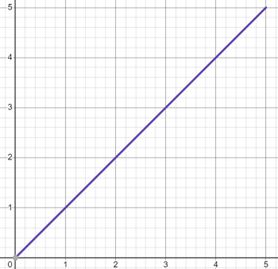
\includegraphics[width=0.7\textwidth]{pic/711.png}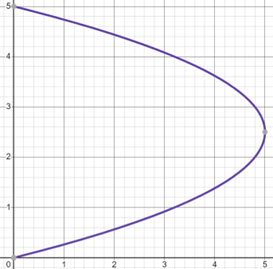
\includegraphics[width=0.7\textwidth]{pic/712.png}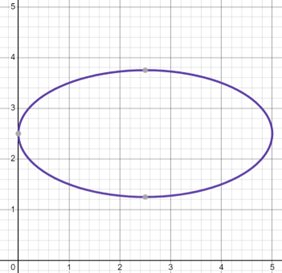
\includegraphics[width=0.7\textwidth]{pic/713.png} }
\end{minipage}
\end{figure}

---------------

Автор -- Тимур Гонтарь, М3206\question
Приведите  пример  нескольких бинарных отношений:
\begin{enumerate}
	\renewcommand{\labelenumi}{\alph{enumi})}
	\item отношение, которое является композиции нескольких бинарных отношений,  которое  нестрого порядка  и антисимметрично (укажите все бинарные отношения, участвующие в композиции)
	\item отношение, которое частично упорядочивает множество и как минимум 7 элементов упорядочены (обязательно покажите порядок элементов множества, полученный упордочиванием бинарным отношением)
	\item отношение, такое что обратное к нему  обладает одинаковыми с ним свойствами и оба антирефлексивны и симметричны (докажите, что свойства сохранаются)
\end{enumerate}

\underline{примечание:} важно показать  множества, на которых задано бинарное отношение и доказать, что ваше бинарное отношение обладает заданными свойствами
\question
Петя решил поучаствовать в конкурсе рисунков, к сожалению, проблема была в том, что он совершенно не умел рисовать, но Петя был умным мальчиком, который знал бинарные отношения.
\\На декартовом произведении множества $A = \{-2, -1, 0, 1, 2, 3, 4, 5, 6, 7, 8, 9, 10, 11\}$ заданы бинарные отношения:
\begin{equation*}
R_1 = {(0, -2), (2, 0), (6, -2), (8, 0), (9, -2), (12, -2), (11, -1), (11, 1), (12, 2), (9, 2), (8, 0), (6, 2), (5, 5), (0, 5), (6, 7), (0, 6)}
\end{equation*}
\begin{center}и\end{center}
\begin{equation*}
R_2 = \{(10, -1), (10, -1), (9, 0)\}
\end{equation*}
Помогите Пете выиграть в конкурсе! Постройте композиции отношений $R_1^{-1}, R_2^{-1}$ и изобразите полученный результат на декартовой системе координат (задание можно дополнять другими композициями).
\\
---------------

Автор -- Анастасия Стеценко, М3207\question
Даны отношения $R_1$, $R_2$ и $R_3$ на множестве $A = \{1; 2; 3; 4; 5;\}$ 
\begin{enumerate}
	\renewcommand{\labelenumi}{\alph{enumi})}
	\item $R_1 = \{(3; 2); (3; 1); (1; 3)\}$
	\item $R_2 = \{(1; 2); (2; 2); (1; 3); (4; 5)\}$
	\item $R_3 = \{(1; 2); (2; 2); (3; 4); (3; 5); (4; 5)\}$
\end{enumerate}

\begin{enumerate}
	\renewcommand{\labelenumi}{\alph{enumi})}
	\item $R_1 \cap R_2^{-1} \cup R_3^2$
	\item $(R_1 \cup R_2) \cap R_3$
	\item $R_3^2 \cap R_3^{-1}$
	\item $R_3^{-1} \cup \overline{R_2^{-1}}$
	\item $R_1^{-1} \cup \overline{R_2} \cup R_3$
\end{enumerate}

определите основные свойства, получившихся отношений
определите какие свойства сохраняются относительно исходных отношений $R_1$, $R_2$ и $R_3$ 

\underline{примечание:} результатом может быть пустое множество

\end{questions}
\newpage
%%% begin test
\begin{flushright}
\begin{tabular}{p{2.8in} r l}
%\textbf{\class} & \textbf{ФИО:} & \makebox[2.5in]{\hrulefill}\\
\textbf{\class} & \textbf{ФИО:} &Дополнительный 2
\\

\textbf{\examdate} &&\\
%\textbf{Time Limit: \timelimit} & Teaching Assistant & \makebox[2in]{\hrulefill}
\end{tabular}\\
\end{flushright}
\rule[1ex]{\textwidth}{.1pt}


\begin{questions}
\question
Вы -- великая искательница сокровищ Лариса Крафтовое. Очередное путешествие забросило вас в подземные гробницы Сигизмунда I. К сожалению, на вашем пути встал очень назойливый мраморный привратник, который по всем канонам жанра имеет для вас пару загадок.
\\
\\
Привратник загадывает свое множество $X$, а также дает вам парочку других $(A,B,C…)$, объединяя, пересекая, дополняя и/или выполняя разность над которыми вы должны получить его множество. Загвоздка лишь в том, что привратник сам выбирает расстановку множеств в формуле, поэтому вам остается лишь вставить операции и расставить скобки (при надобности).

\paragraph{Загадка 1:}
\begin{equation*}
    X=\{2,3\}
\end{equation*}
\begin{equation*}
    A=\{1,2,3\}; B=\{3,4,5\}; C=\{1,4,5\}; D=\{2,3,5\}
    \end{equation*}
\begin{equation*}
    A ? B ? C ? D ? A ? C = X
\end{equation*}

\paragraph{Загадка 2:}
\begin{equation*}
    X=\{5,6\}
\end{equation*}
\begin{equation*}
    A=\{1,2,3,4\}; B=\{2,4,6\}; C=\{1,3,5\}
    \end{equation*}
\begin{equation*}
    A ? B ? C ? A = X
\end{equation*}

---------------

Автор -- Константин Васильев, М3213\question
Упростите следующее выражение с учетом того, что $A\subset B \subset C \subset D \subset U; A \neq \emptyset$
\begin{equation*}
	A \cap C  \cap D \cup B \cap \overline{C} \cap D \cup B \cap C \cap D
\end{equation*}

Примечание: $U$ -- универсум\question
Укажите номера множеств, являющихся подмножествами множества
\begin{equation*}
	Q = \bar{A} \cup B \cap C \cup \bar{C} \cap \bar{D}
\end{equation*}

\begin{enumerate}
	\renewcommand{\labelenumi}{\arabic{enumi})}
	\item $P = A \cap \bar{B} \cap D \cup \bar{A} \cap \bar{B} \cap C$;
	\item $P = A \cap B \cap D \cup \bar{A} \cap \bar{C} \cap D$;
	\item $P = B \cap \bar{C} \cap \bar{D} \cup A \cap B \cap \bar{C}$;
	\item $P = A \cap \bar{C} \cap \bar{D} \cup \bar{A} \cap \bar{B} \cap D$.
\end{enumerate}
\question
Постройте разбиения множеств:
\begin{enumerate}
	\renewcommand{\labelenumi}{\alph{enumi})}
	\item $A = \{6, 7, 8, 9, 11, 14, 34, 91, 55, 65, 76, 28, 19\};$
	\item $B = \{0, 1, 2, 3, 4, 8, 9, 11, 22, 33, 44, 55, 65, 76, 28, 19\}$
	\item $A \cup B$
	\item $A \cap B$
\end{enumerate}
Таким образом, чтобы все разбиения имели как минимум 2 одинаковых множества в разбиениях.
Мощность каждого разбиение была более 4.
Докажите, что ваш ответ соответствует указанным условиям!\question
Пусть у нас есть $P$ -- множество студентов города Санкт-Петербург, из них $A$ -- третьекурсники, $B$ -- проходят профессиональную переподготовку, а $C$ -- стажируются в Яндексе. Для статьи “Как учиться на третьем курсе университета ИТМО, проходить профессиональную подготовку и не умереть” Мегабайт создал выборку $D$.
\\
\\
Упростите множество $E = (P \cap D \cup C \cap \overline{B} \cap \overline{D} \cup B \cap A \cap \overline{C}) \cap \overline{C} \cap \overline{D} \cap P$, а затем опишите его словами.
\\
\\
---------------

Автор -- Антонина Чернова, М33081\question
Бабушка Люда потеряла книгу со своими лучшими рецептами напитков. Вы, как добросовестный внук, проводивший у любимой бабушки большое количество времени, помните из чего бабуля варила вкуснейшие морсы и компоты. Обычно бабушка варила напитки из двух видов ягод и фруктов среди которых были: Малина, Облепиха, Жимолость, Смородина, Яблоки, Абрикосы и Груши. Также вы помните, что нельзя совмещать между собой Облепиху и красные ягоды, Абрикос и ягоды, Яблоко и ягоды. Постройте бинарное отношение содержащее все возможные сочетания для напитков таким образом, чтобы ингредиенты не повторялись.
\\
Ответьте на вопросы касаемо построенного бинарного отношения:
\begin{itemize}
    \item Какими свойствами обладает данное БО? Обоснуйте
    \item Является ли данное отношение функциональным?
    \item Каким из отношений соответствия оно является? (одно-многозначным, много-многозначным и т.д.)
\end{itemize}
\\
---------------

Автор -- Максим Акимцов, М3208\question
Одним теплым вечером кот Степан вдохновился картинами, которые он увидел в Эрмитаже, и решил нарисовать свой автопортрет. Так как у Степана была тетрадка в клетку, оставшаяся после пройденного курса дискретной математики, он решил рисовать там. Нарисовав автопортрет ровно по клеткам, он подумал, что можно дорисовать координатные оси и обозначить все целые точки, пересекающиеся с контуром портрета. На обратной стороне листка он увидел конспект лекции по бинарным отношениям. Но так как память у кота не очень хорошая, он решил попросить вас найти бинарное отношение, соответствующее рисунку и два таких бинарных отношения, чтобы в композиции они давали исходное бинарное отношение и изобразить их.
\\
\begin{figure}[h]

\begin{minipage}[h]{0.55\linewidth}
\end{minipage}
\begin{minipage}[h]{0.45\linewidth}
\center{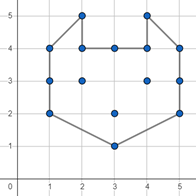
\includegraphics[width=0.7\textwidth]{pic/721.png} }
\end{minipage}
\end{figure}



---------------

Автор -- Алёна Холмогорова, М3209\question
Приведите  пример  нескольких бинарных отношений:
\begin{enumerate}
	\renewcommand{\labelenumi}{\alph{enumi})}
	\item отношение, которое является композиции нескольких бинарных отношений,  которое  обладает любым типом соответсвия  и симметрично (укажите все бинарные отношения, участвующие в композиции)
	\item два отношения, первое -- частично упорядочивает множество, на котором оно задано и второе -- полностью упорядочивает (обязательно покажите порядок элементов множества, полученный упордочиванием бинарным отношением)
	\item отношение, такое что обратное к нему  обладает одинаковыми с ним свойствами и оба функциональны (докажите, что свойства сохранаются)
\end{enumerate}

\underline{примечание:} важно показать  множества, на которых задано бинарное отношение и доказать, что ваше бинарное отношение обладает заданными свойствами
\question
Два контрабандиста затеяли сделку. Им кажется, что все должно пройти гладко и их план идеален, но стражи порядка уже взялись за это дело и планируют встать между ними, сорвав аферу. $\{1, 2, 3, 0\}$ – товары, которые планирует передать контрабандист $A$. $\{1, 2, 3, 4\}$ – планирует передать $B$. $A$, ничего не подозревая, уже готов передать две штуки товара 1 в руки полицейскому (притворившегося контрабандистом $B$) в обмен на 1 и 3 товар подставного $B$, две штуки товарa 2 – тоже в обмен на 1 и 3 товар. Также полиция связалась с $B$ по поводу передачи товара 3 в обмен на 4, и 3 на 1. Таким образом, если у полиции получилось перехватить сделки с обоих концов – работа выполена, и товар не окажется в руках ни у $A$ ни у $B$. Какие и сколько сделок полиции удалось предотвратить?
\\
---------------

Автор -- Мария Баженова, М3219\question
Даны отношения $R_1$, $R_2$ и $R_3$ на множестве $A = \{1; 2; 3; 4; 5;\}$ 
\begin{enumerate}
	\renewcommand{\labelenumi}{\alph{enumi})}
	\item $R_1 = \{(1; 1); (2; 2); (3; 3); (2; 1); (1; 2); \}$
	\item $R_2 = \{(1; 1); (2; 2); (1; 3); (3; 4); (3; 5);\}$
	\item $R_2 = \{(1; 1); (2; 2);  (1; 5); (3; 4); (3; 5); (4; 5)\}$
\end{enumerate}

\begin{enumerate}
	\renewcommand{\labelenumi}{\alph{enumi})}
	\item $R_1 \cap R_2$
	\item $R_1 \cup R_2 \cup R_3$
	\item $R_1^2 \cap R_3^{-1}$
	\item $R_1 \cup R_3^4$
	\item $R_1 \cup \overline{R_3}$
\end{enumerate}

определите основные свойства, получившихся отношений
определите какие свойства сохраняются относительно исходных отношений $R_1$, $R_2$ и $R_3$ 

\underline{примечание:} результатом может быть пустое множество

\end{questions}
\newpage
%%% begin test
\begin{flushright}
\begin{tabular}{p{2.8in} r l}
%\textbf{\class} & \textbf{ФИО:} & \makebox[2.5in]{\hrulefill}\\
\textbf{\class} & \textbf{ФИО:} &Дополнительный 3
\\

\textbf{\examdate} &&\\
%\textbf{Time Limit: \timelimit} & Teaching Assistant & \makebox[2in]{\hrulefill}
\end{tabular}\\
\end{flushright}
\rule[1ex]{\textwidth}{.1pt}


\begin{questions}
\question
Вы -- великая искательница сокровищ Лариса Крафтовое. Очередное путешествие забросило вас в подземные гробницы Сигизмунда I. К сожалению, на вашем пути встал очень назойливый мраморный привратник, который по всем канонам жанра имеет для вас пару загадок.
\\
\\
Привратник загадывает свое множество $X$, а также дает вам парочку других $(A,B,C…)$, объединяя, пересекая, дополняя и/или выполняя разность над которыми вы должны получить его множество. Загвоздка лишь в том, что привратник сам выбирает расстановку множеств в формуле, поэтому вам остается лишь вставить операции и расставить скобки (при надобности).

\paragraph{Загадка 1:}
\begin{equation*}
    X=\{2,3\}
\end{equation*}
\begin{equation*}
    A=\{1,2,3\}; B=\{3,4,5\}; C=\{1,4,5\}; D=\{2,3,5\}
    \end{equation*}
\begin{equation*}
    A ? B ? C ? D ? A ? C = X
\end{equation*}

\paragraph{Загадка 2:}
\begin{equation*}
    X=\{5,6\}
\end{equation*}
\begin{equation*}
    A=\{1,2,3,4\}; B=\{2,4,6\}; C=\{1,3,5\}
    \end{equation*}
\begin{equation*}
    A ? B ? C ? A = X
\end{equation*}

---------------

Автор -- Константин Васильев, М3213\question
Упростите следующее выражение с учетом того, что $A\subset B \subset C \subset D \subset U; A \neq \emptyset$
\begin{equation*}
	\overline{A} \cap \overline{C} \cap D \cup \overline{B} \cap \overline{C} \cap D \cup A \cap B
\end{equation*}

Примечание: $U$ -- универсум\question
Укажите номера множеств, являющихся подмножествами множества
\begin{equation*}
	Q = A \cap \bar{D} \cup B \cap C \cup \bar{A} \cap \bar{B} \cap D \cup A \cap C
\end{equation*}

\begin{enumerate}
	\renewcommand{\labelenumi}{\arabic{enumi})}
	\item $P = B \cap C \cap D \cup \bar{A} \cap B \cap C$;
	\item $P = \bar{B} \cap \bar{C} \cap D \cup B \cap \bar{C} \cap \bar{D}$;
	\item $P = A \cap \bar{B} \cap D \cup A \cap C \cap D$;
	\item $P = \bar{B} \cap \bar{C} \cup \bar{A} \cap \bar{B} \cap D$.
\end{enumerate}
\question
Постройте разбиения множеств:
\begin{enumerate}
	\renewcommand{\labelenumi}{\alph{enumi})}
	\item $A = \{6, 7, 8, 9, 11, 14, 34, 54, 47, 18, 91, 55, 65, 76, 28, 19\};$
	\item $B = \{0, 11, 14, 34, 22, 33, 44, 55, 65, 76, 28, 19\}$
	\item $A \cup B$
	\item $A \cap B$
\end{enumerate}
Таким образом, чтобы все разбиения имели как минимум 2 одинаковых множества в разбиениях.
Мощность каждого разбиение была более 5.
Докажите, что ваш ответ соответствует указанным условиям!
\question
Докажите, что два выражения равны.

\begin{equation}
    (A \cup B) \backslash C = (A \backslash C) \cup (B \backslash C)
\end{equation}

\begin{equation}
    (A \backslash B) \cap C = (A \cap C) \backslash (B \cap C)
\end{equation}

\begin{equation}
    A \times (B \cap C) = (A \times B) \cap (A \times C)
\end{equation}

\begin{equation}
    A \times (B \cup C) = (A \times B) \cup (A \times C)
\end{equation}
\\
\\
$\times$ -- декартово произведение
\\
---------------

Автор -- Алексей Лёвушкин, М3204\question
Возьмём множество $M = \{1, 2, 3, 4, 5, 6, 7, 8, 9\}$. Определите свойства и виды бинарных отношений:
\begin{itemize}
    \item $xRy \Leftrightarrow x$ делит $y$
    \item $xRy \Leftrightarrow x + y = 8$
    \item $xRy \Leftrightarrow x + y \in M$
\end{itemize}
---------------

Автор -- Алексей Лёвушкин, М3204\question
Приведите доказательства следующих утверждений:
\begin{itemize}
    \item Доказать, что отношение «равенство по модулю 5» является отношением эквивалентности на множестве целых чисел.
    \item Докажите, что всякое отношение строгого порядка является асимметричным.
    \item R задано на декартовом квадрате натуральных чисел. Пара $(m,n)$ принадлежит отношению $R$, если $n^3 + 3m^2 + 2m$ делится на 6. Докажите, что это - отношение эквивалентности.
\end{itemize}
\\
---------------

Автор -- разные студенты потока ИС2026\question
Пусть имеется бинарное отношение $R$ на $ A \times A$. Докажите, что если $R$ -- одновременно и отношение эквивалентности и отношение частичного порядка, то оно -- отношение равенства.
\\
---------------

Автор -- Алексей Ващенков, М3205\question
Довольные студенты ИТМО сдали летнюю сессию и намерены поехать домой на некоторое время. К сожалению, чтобы добраться до пункта назначения, им потребуется сделать несколько пересадок.

Пусть множество всех населенных пунктов выглядит как: $A = \{1, 2, 3, 4, 5, 6\}$.
\\
Тогда $R = \{(1, 3), (3, 1), (2, 4), (4, 2), (1, 5), (5, 1), (2, 3), (3, 2)\}$ -- можно доехать на автобусе, $S = \{(5, 6), (6, 5), (3, 6), (6, 3)\}$ -- можно долететь на самолете.

\begin{itemize}
    \item Найдите такие пары пунктов, для перемещения между которыми надо проехать на автобусе, а затем воспользоваться самолетом и наоборот.
    \item Найдите пары пунктов, между которыми можно перемещаться на автобусе с одной пересадкой (пары вида (1, 1) не стоит указывать в ответе).
    \item Найдите пары пунктов, между которыми можно перемещаться на самолете с одной пересадкой в промежуточном пункте.
\end{itemize}
\\
---------------

Автор -- Елизавета Котельникова, М3212\question
Даны отношения $R_1$, $R_2$ и $R_3$ на множестве $A = \{1; 2; 3; 4; 5;\}$ 
\begin{enumerate}
	\renewcommand{\labelenumi}{\alph{enumi})}
	\item $R_1 = \{(3; 2); (3; 1); (1; 3)\}$
	\item $R_2 = \{(1; 2); (2; 2); (1; 3); (1; 5); (2; 3); (4; 5)\}$
	\item $R_2 = \{(1; 2); (2; 2); (3; 4); (3; 5); (4; 5)\}$
\end{enumerate}

\begin{enumerate}
	\renewcommand{\labelenumi}{\alph{enumi})}
	\item $R_1 \cap R_2$
	\item $(R_1 \cup R_2) \cap R_3$
	\item $R_3^2 \cap R_3^{-1}$
	\item $R_3 \cup \overline{R_2^2}$
	\item $R_1 \cup \overline{R_2} \cup R_3$
\end{enumerate}

определите основные свойства, получившихся отношений
определите какие свойства сохраняются относительно исходных отношений $R_1$, $R_2$ и $R_3$ 

\underline{примечание:} результатом может быть пустое множество

\end{questions}
\newpage
%%% begin test
\begin{flushright}
\begin{tabular}{p{2.8in} r l}
%\textbf{\class} & \textbf{ФИО:} & \makebox[2.5in]{\hrulefill}\\
\textbf{\class} & \textbf{ФИО:} &Дополнительный 4
\\

\textbf{\examdate} &&\\
%\textbf{Time Limit: \timelimit} & Teaching Assistant & \makebox[2in]{\hrulefill}
\end{tabular}\\
\end{flushright}
\rule[1ex]{\textwidth}{.1pt}


\begin{questions}
\question
Ребята приехали в математический лагерь, где каждый получил футболку с уникальным номером от 1 до 23. Отправившись на очередной полдник, они обнаружили, что нет ни одного кекса – их украли! Ребята сразу приступили к расследованию. Таким образом, они сделали вывод, что виновник – не один человек, а целая группа! У них получилось разделить всех ребят на 4 группы подозреваемых, в зависимости от того, кто где был в предположительное время совершения преступления по словам очевидцев.
\\(Легенда: С – столовая, D – двор, B – баскетбольная площадка, А - аллея): 
\begin{center}
$A: \{1, 2, 3, 21, 23, 5, 22, 18, 19, 6\}$
\\
$B: \{6, 22, 10, 15, 11, 13, 7, 18, 14, 9\}$
\\
$C: \{7, 8, 14, 20, 12, 4, 1, 2, 19, 6\}$
\\
$D: \{9, 13, 16, 17, 18, 19, 22, 14, 5, 6\}$
\end{center}
Так как ребята были отличными математиками, у них получилось составить выражение, которое раскроет, кто виноват в преступлении. 
\begin{equation*}
    A \cup B \cap \overline{C} \cup (A \cap D \cup \overline{C}) \cup D
\end{equation*}
Помогите им найти виновных.

---------------

Автор -- Баженова Мария, М3219\question
Упростите следующее выражение с учетом того, что $A\subset B \subset C \subset D \subset U; A \neq \emptyset$
\begin{equation*}
	\overline{A} \cap \overline{C} \cap D \cup \overline{B} \cap \overline{C} \cap D \cup A \cap B
\end{equation*}

Примечание: $U$ -- универсум\question
Укажите номера множеств, являющихся подмножествами множества
\begin{equation*}
	Q = \bar{A} \cap C \cup A \cap \bar{B} \cup A \cap \bar{C} \cup \bar{A} \cap B \cap D
\end{equation*}

\begin{enumerate}
	\renewcommand{\labelenumi}{\arabic{enumi})}
	\item $P = A \cap \bar{B} \cap D \cup \bar{A} \cap \bar{B} \cap C$;
	\item $P = A \cap B \cap D \cup \bar{A} \cap \bar{C} \cap D$;
	\item $P = B \cap \bar{C} \cap \bar{D} \cup A \cap B \cap \bar{C}$;
	\item $P = A \cap \bar{C} \cap \bar{D} \cup \bar{A} \cap \bar{B} \cap D$.
\end{enumerate}
\question
Постройте разбиения множеств:
\begin{enumerate}
	\renewcommand{\labelenumi}{\alph{enumi})}
	\item $A = \{6, 7, 8, 9, 11, 14, 34, 54, 47, 18, 91\};$
	\item $B = \{0, 1, 2, 3, 4, 5, 6, 7, 8, 9\}$
	\item $A \cap B$
\end{enumerate}
Таким образом, чтобы все разбиения имели как минимум 2 одинаковых множества в разбиениях.
Мощность каждого разбиение была более 3.
Докажите, что ваш ответ соответствует указанным условиям!\question
Упростить выражения, используя свойства операций над множествами:

\begin{enumerate}
	\renewcommand{\labelenumi}{\alph{enumi})}
	\item $(\bar{A} \cup B \cup \bar{C}) \cap(A \cap \bar{B} \cap C) \cap \overline{(A \cup C)}$;
	\item $(A\cap B \cap C \cap D) \cup (\overline{\overline{A}\cup C}\cap D) \cup (D\cap\overline{(\overline{A}+C)+D})\cup (\overline{A}\cap B\cap C \cap D)$.
\end{enumerate}
\question
Бабушка Люда потеряла книгу со своими лучшими рецептами напитков. Вы, как добросовестный внук, проводивший у любимой бабушки большое количество времени, помните из чего бабуля варила вкуснейшие морсы и компоты. Обычно бабушка варила напитки из двух видов ягод и фруктов среди которых были: Малина, Облепиха, Жимолость, Смородина, Яблоки, Абрикосы и Груши. Также вы помните, что нельзя совмещать между собой Облепиху и красные ягоды, Абрикос и ягоды, Яблоко и ягоды. Постройте бинарное отношение содержащее все возможные сочетания для напитков таким образом, чтобы ингредиенты не повторялись.
\\
Ответьте на вопросы касаемо построенного бинарного отношения:
\begin{itemize}
    \item Какими свойствами обладает данное БО? Обоснуйте
    \item Является ли данное отношение функциональным?
    \item Каким из отношений соответствия оно является? (одно-многозначным, много-многозначным и т.д.)
\end{itemize}
\\
---------------

Автор -- Максим Акимцов, М3208\question
Дана декартова система координат. Ось $x$ представляет собой множество $X$, ось $y$ - множество $Y$. На этих двух множествах определены бинарные отношения, которые схематически изображены в виде графиков выше (то есть, например, для графика с рис. 1 будет верно, что пары $(0, 0), (1, 1), (2, 2), (3, 3), (4, 4), (5, 5)$ входят в бинарное отношение, соответствующее графику). Для каждого из таких отношений определить:
\begin{itemize}
    \item Каким типом отношения соответствия оно является?
    \item Является ли оно функциональным отношением? Если да, то каким именно (сюръекция, инъекция, биекция)?
\end{itemize}
Обоснуйте своё решение. После этого, аналогично данным в условии графикам, придумайте отношение (любое), которое будет представлять собой полностью определенную функцию, и при этом будет инъективно и не сюръективно.
\\
\begin{figure}[h]

\begin{minipage}[h]{0.55\linewidth}
\end{minipage}
\begin{minipage}[h]{0.45\linewidth}
\center{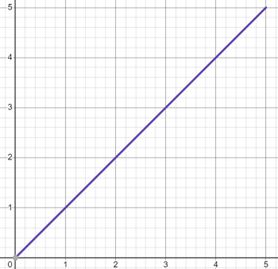
\includegraphics[width=0.7\textwidth]{pic/711.png}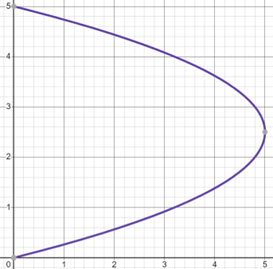
\includegraphics[width=0.7\textwidth]{pic/712.png}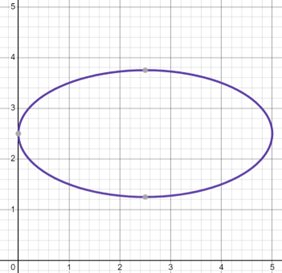
\includegraphics[width=0.7\textwidth]{pic/713.png} }
\end{minipage}
\end{figure}

---------------

Автор -- Тимур Гонтарь, М3206\question
Пусть $A = \{a, b, c, 1, \Delta\}$. Рассмотрим следующее отношение R:

\begin{equation*}
R = \{(a, a), (b, b), (c, c), (1, 1),
(\Delta, \Delta), (a, b), (b, 1), (a, 1),
(a, \Delta), (b, \Delta), (a, c), (c, \Delta)\}
\end{equation*}
\begin{itemize}
    \item Докажите, что R -- отношение порядка.
    \item У каких из следующих множеств есть наибольший/наименьший элемент?
    \begin{itemize}
        \item $X_1 = \{b, 1, \Delta\}$
        \item $X_2 = \{b, c, \Delta\}$
        \item $X_3 = \{1, c, \Delta\}$
        \item $X_4 = \{a, b, c, \Delta\}$
        \item $X_5 = \{1, c\}$
        \item $X_6 = \{ \Delta \}$
        \item $X_7 = \{b, c\}$
    \end{itemize}
    \item Полностью или частично упорядочите множество А.
\end{itemize}
\\
---------------

Автор -- Алексей Ващенков, М3205\question
В перерыве между парами дискретной математики вы с друзьями решили зарубиться в домино. Иллюстрация ниже визуализирует данный момент игры.

\\
\begin{figure}[h]

\begin{minipage}[h]{0.55\linewidth}
\end{minipage}
\begin{minipage}[h]{0.45\linewidth}
\center{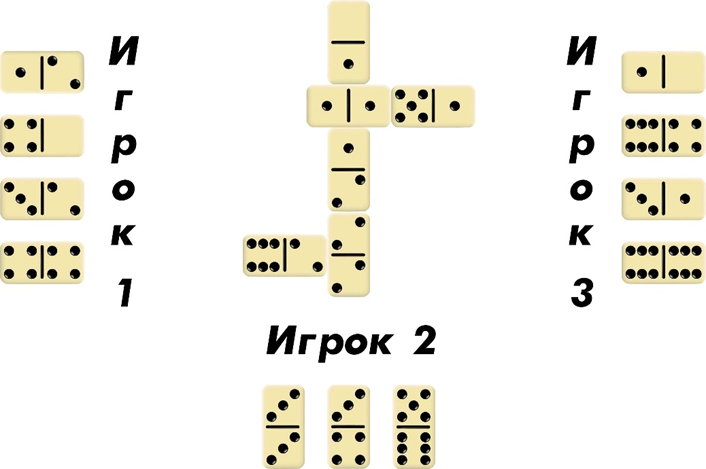
\includegraphics[width=0.7\textwidth]{pic/941.png} }
\end{minipage}
\end{figure}

Так как вы — умные студенты, вам стало интересно интерпретировать партию в виде бинарных отношений. Запишите отношения:
\begin{itemize}
    \item $G = \{(a,b)|a$ и $b$ – стороны свободных доминошек, лежащих на столе, где a – свободная сторона$\}$
    \item $R_1 = \{(a,b)|a$ и $b$ – стороны одной доминошки в руке у первого игрока$\}$
    \item $R_2 = \{(a,b)|a$ и $b$ – стороны одной доминошки в руке у второго игрока$\}$
    \item $R_3 = \{(a,b)|a$ и $b$ – стороны одной доминошки в руке у третьего игрока$\}$
\end{itemize}

Используя операцию композиции, составьте новые бинарные отношения:
\begin{itemize}
    \item $P_1$ – возможные ходы у первого игрока
    \item $P_2$ – возможные ходы у второго игрока
    \item $P_3$ – возможные ходы у третьего игрока
\end{itemize}


Ходом является пара крайних номеров стоящих рядом доминошек.
\\
---------------

Автор -- Константин Васильев, М3213\question
Даны отношения $R_1$, $R_2$ и $R_3$ на множестве $A = \{1; 2; 3; 4; 5;\}$ 
\begin{enumerate}
	\renewcommand{\labelenumi}{\alph{enumi})}
	\item $R_1 = \{(2; 1); (1; 2); (2; 3); (3; 2); (3; 1); (1; 3)\}$
	\item $R_2 = \{(1; 2); (2; 2); (1; 3); (1; 5); (2; 3); (2; 4); (2; 5); (4; 5)\}$
	\item $R_3 = \{(1; 2); (2; 2); (1; 3); (1; 5); (3; 4); (3; 5); (4; 5)\}$
\end{enumerate}

\begin{enumerate}
	\renewcommand{\labelenumi}{\alph{enumi})}
	\item $\overline{R_1} \cap R_2^{-1} \cap R_3$
	\item $(R_1^3 \cup R_2) \cap R_3^{-1}$
	\item $R_3 \cap R_3^{-1}$
	\item $R_3^{-1} \cup \overline{R_2^{-1}}$
	\item $R_1^{-1} \cup \overline{R_2} \cup R_3$
\end{enumerate}

определите основные свойства, получившихся отношений
определите какие свойства сохраняются относительно исходных отношений $R_1$, $R_2$ и $R_3$ 

\underline{примечание:} результатом может быть пустое множество

\end{questions}
\newpage
%%% begin test
\begin{flushright}
\begin{tabular}{p{2.8in} r l}
%\textbf{\class} & \textbf{ФИО:} & \makebox[2.5in]{\hrulefill}\\
\textbf{\class} & \textbf{ФИО:} &Дополнительный 5
\\

\textbf{\examdate} &&\\
%\textbf{Time Limit: \timelimit} & Teaching Assistant & \makebox[2in]{\hrulefill}
\end{tabular}\\
\end{flushright}
\rule[1ex]{\textwidth}{.1pt}


\begin{questions}
\question
В самом мирном городе мира, Лос-Сантосе, орудуют несколько бандитских группировок: Гроув-стрит, Баллос и Вагос. Некоторые районы города, для удобства бандитов помеченные цифрами \{0...9\}, находятся под влиянием этих банд:
\begin{itemize}
    \item Гроув-стрит: \{1, 2, 3, 7, 9\}
    \item Баллос: \{1, 3, 7, 8\}
    \item Вагос: \{4, 6, 7, 9\}
\end{itemize}
Районы, оказавшиеся под влиянием нескольких банд, называются спорными территориями.
\\
\\
В один прекрасный летний день Си-Джей увидел на стене своего дома граффити с сообщением от информатора из банды Баллосов. Для конспирации он оставил его в таком виде:
\begin{equation*}
B \cap \overline{G} \cup G \cap V \cap \overline{B} \cup G \cap B \cap \overline{V}
\end{equation*}
В нем содержатся номера районов, на которые полиция планирует совершить облаву. Вам, как самому умному представителю Гроув-Стрит, необходимо расшифровать граффити, а затем ответить на следующие вопросы:

\begin{itemize}
    \item Какие районы являются спорными территориями, под влиянием двух или трех банд?
    \item Какие районы полностью находятся под влиянием банды Вагос, без участия других банд?
    \item На какие из районов полиция не планирует совершать облаву?
\end{itemize}

---------------

Автор -- Константин Васильев, М3213\question
Упростите следующее выражение с учетом того, что $A\subset B \subset C \subset D \subset U; A \neq \emptyset$
\begin{equation*}
	A \cap B \cup \overline{A} \cap \overline{C} \cup A \cap C \cup \overline{B} \cap \overline{C}
\end{equation*}

Примечание: $U$ -- универсум\question
Укажите номера множеств, являющихся подмножествами множества
\begin{equation*}
	Q = A \cap \bar{D} \cup B \cap C \cup \bar{A} \cap \bar{B} \cap D \cup A \cap C
\end{equation*}

\begin{enumerate}
	\renewcommand{\labelenumi}{\arabic{enumi})}
	\item $P = A \cap \bar{B} \cap D \cup \bar{A} \cap \bar{B} \cap C$;
	\item $P = A \cap B \cap D \cup \bar{A} \cap \bar{C} \cap D$;
	\item $P = B \cap \bar{C} \cap \bar{D} \cup A \cap B \cap \bar{C}$;
	\item $P = A \cap \bar{C} \cap \bar{D} \cup \bar{A} \cap \bar{B} \cap D$.
\end{enumerate}
\question
Постройте разбиения множеств:
\begin{enumerate}
	\renewcommand{\labelenumi}{\alph{enumi})}
	\item $A = \{6, 7, 8, 9, 11, 14, 34, 54, 91\};$
	\item $B = \{0, 1, 2, 3, 4, 5, 6, 7, 8, 9\}$
	\item $A \cap B$
\end{enumerate}
Таким образом, чтобы все разбиения имели как минимум 2 одинаковых множества в разбиениях.
Мощность каждого разбиение была более 6.
Докажите, что ваш ответ соответствует указанным условиям!\question
Пусть у нас есть $P$ -- множество студентов города Санкт-Петербург, из них $A$ -- третьекурсники, $B$ -- проходят профессиональную переподготовку, а $C$ -- стажируются в Яндексе. Для статьи “Как учиться на третьем курсе университета ИТМО, проходить профессиональную подготовку и не умереть” Мегабайт создал выборку $D$.
\\
\\
Упростите множество, используя свойства операций и комментируя каждый шаг, а затем опишите его словами.
\begin{equation*}
    \overline{\overline{A} \cap \overline{B}} \cap (A \cap \overline{\overline{B} \cup \overline{C}} \cup \overline{\overline{A} \cup \overline{B} \cup \overline{C}}) \cup D
\end{equation*}
\\
---------------

Автор -- Антонина Чернова, М33081\question
Возьмём множество $M = \{1, 2, 3, 4, 5, 6, 7, 8, 9\}$. Определите свойства и виды бинарных отношений:
\begin{itemize}
    \item $xRy \Leftrightarrow x$ делит $y$
    \item $xRy \Leftrightarrow x + y = 8$
    \item $xRy \Leftrightarrow x + y \in M$
\end{itemize}
---------------

Автор -- Алексей Лёвушкин, М3204\question
Установите, является ли каждое из перечисленных ниже отношений на А ($R \subseteq A \times A$) отношением эквивалентности (обоснование ответа обязательно). Для каждого отношения эквивалентности постройте классы 
эквивалентности и постройте граф отношения:
\begin{enumerate}
	\renewcommand{\labelenumi}{\alph{enumi})}
	\item Пусть A -- множество имен. $A = \{ $Алексей, Иван, Петр, Александр, Павел, Андрей$ \}$. Тогда отношение $R$ верно на парах имен, начинающихся с одной и той же буквы, и только на них.
	\item $A = \{-10, -9, ..., 9, 10\}$ и отношение $ R = \{(a,b)|a^{2} = b^{2}\}$
	\item На множестве $A = \{1; 2; 3\}$ задано отношение $R = \{(1; 1); (2; 2); (3; 3); (3; 2); (1; 2); (2; 1)\}$
\end{enumerate}\question
Пусть $A = \{a, b, c, 1, \Delta\}$. Рассмотрим следующее отношение R:

\begin{equation*}
R = \{(a, a), (b, b), (c, c), (1, 1),
(\Delta, \Delta), (a, b), (b, 1), (a, 1),
(a, \Delta), (b, \Delta), (a, c), (c, \Delta)\}
\end{equation*}
\begin{itemize}
    \item Докажите, что R -- отношение порядка.
    \item У каких из следующих множеств есть наибольший/наименьший элемент?
    \begin{itemize}
        \item $X_1 = \{b, 1, \Delta\}$
        \item $X_2 = \{b, c, \Delta\}$
        \item $X_3 = \{1, c, \Delta\}$
        \item $X_4 = \{a, b, c, \Delta\}$
        \item $X_5 = \{1, c\}$
        \item $X_6 = \{ \Delta \}$
        \item $X_7 = \{b, c\}$
    \end{itemize}
    \item Полностью или частично упорядочите множество А.
\end{itemize}
\\
---------------

Автор -- Алексей Ващенков, М3205\question
Вася хочет устроиться бэкенд разработчиком в ИТМО, работать с ИСУ. На собеседовании тимлид дал ему тестовое задание, чтобы определить его уровень знаний:
\\
\begin{figure}[h]

\begin{minipage}[h]{0.55\linewidth}
\end{minipage}
\begin{minipage}[h]{0.45\linewidth}
\center{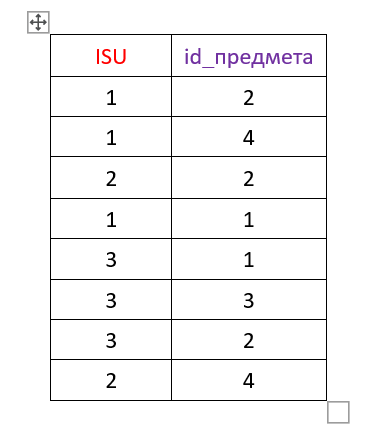
\includegraphics[width=0.7\textwidth]{pic/911.png}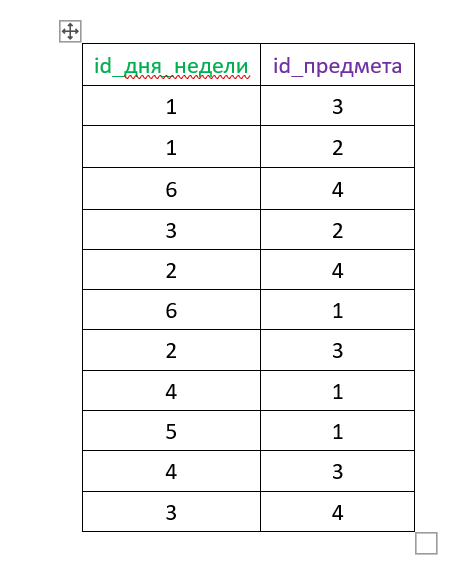
\includegraphics[width=0.7\textwidth]{pic/912.png} }
\end{minipage}
\end{figure}

В базе данных расписания ИТМО есть 2 таблицы:
\begin{itemize}
    \item В таблице 1 (рис. 1) каждому студенту по его номеру ИСУ сопоставлены предметы по их id. У одного номера ИСУ (студента) может быть много предметов, при этом на один предмет может ходить несколько студентов.
    \item В таблице 2 (рис. 2) каждому дню недели по его id (порядковый номер: 1-пн, 2-вт, 3-ср и т. д.) сопоставлены предметы по их id. В один день могут проводиться пары по нескольким предметам, при этом пары по одному предмету могут проходить несколько дней в неделе.
\end{itemize}
От Васи требуется по имеющимся данным вывести все возможные кортежи вида:

\begin{center}(номер ИСУ, день когда у этого студента есть пары)\end{center}

Например, ответ вида $\{(1, 1), (1, 5), (2, 1)\}$ будет означать что студент с ISU №1 имеет пары в понедельник и пятницу, а студент с ISU №2 имеет пары только в понедельник.

Помогите Васе решить данную задачу, используя ваши знания по дискретной математике.

---------------

Автор -- Тимур Гонтарь, М3206\question
Даны отношения $R_1$, $R_2$ и $R_3$ на множестве $A = \{1; 2; 3; 4; 5;\}$ 
\begin{enumerate}
	\renewcommand{\labelenumi}{\alph{enumi})}
	\item $R_1 = \{(2; 1); (1; 2); (2; 3); (3; 2); (3; 1); (1; 3)\}$
	\item $R_2 = \{(1; 2); (2; 2); (1; 3); (1; 5); (2; 3); (2; 4); (2; 5); (4; 5)\}$
	\item $R_3 = \{(1; 2); (2; 2); (1; 3); (1; 5); (3; 4); (3; 5); (4; 5)\}$
\end{enumerate}

\begin{enumerate}
	\renewcommand{\labelenumi}{\alph{enumi})}
	\item $\overline{R_1} \cap R_2^{-1} \cap R_3$
	\item $(R_1^3 \cup R_2) \cap R_3^{-1}$
	\item $R_3 \cap R_3^{-1}$
	\item $R_3^{-1} \cup \overline{R_2^{-1}}$
	\item $R_1^{-1} \cup \overline{R_2} \cup R_3$
\end{enumerate}

определите основные свойства, получившихся отношений
определите какие свойства сохраняются относительно исходных отношений $R_1$, $R_2$ и $R_3$ 

\underline{примечание:} результатом может быть пустое множество

\end{questions}
\newpage
%%% begin test
\begin{flushright}
\begin{tabular}{p{2.8in} r l}
%\textbf{\class} & \textbf{ФИО:} & \makebox[2.5in]{\hrulefill}\\
\textbf{\class} & \textbf{ФИО:} &Дополнительный 6
\\

\textbf{\examdate} &&\\
%\textbf{Time Limit: \timelimit} & Teaching Assistant & \makebox[2in]{\hrulefill}
\end{tabular}\\
\end{flushright}
\rule[1ex]{\textwidth}{.1pt}


\begin{questions}
\question
В самом мирном городе мира, Лос-Сантосе, орудуют несколько бандитских группировок: Гроув-стрит, Баллос и Вагос. Некоторые районы города, для удобства бандитов помеченные цифрами \{0...9\}, находятся под влиянием этих банд:
\begin{itemize}
    \item Гроув-стрит: \{1, 2, 3, 7, 9\}
    \item Баллос: \{1, 3, 7, 8\}
    \item Вагос: \{4, 6, 7, 9\}
\end{itemize}
Районы, оказавшиеся под влиянием нескольких банд, называются спорными территориями.
\\
\\
В один прекрасный летний день Си-Джей увидел на стене своего дома граффити с сообщением от информатора из банды Баллосов. Для конспирации он оставил его в таком виде:
\begin{equation*}
B \cap \overline{G} \cup G \cap V \cap \overline{B} \cup G \cap B \cap \overline{V}
\end{equation*}
В нем содержатся номера районов, на которые полиция планирует совершить облаву. Вам, как самому умному представителю Гроув-Стрит, необходимо расшифровать граффити, а затем ответить на следующие вопросы:

\begin{itemize}
    \item Какие районы являются спорными территориями, под влиянием двух или трех банд?
    \item Какие районы полностью находятся под влиянием банды Вагос, без участия других банд?
    \item На какие из районов полиция не планирует совершать облаву?
\end{itemize}

---------------

Автор -- Константин Васильев, М3213\question
Упростите следующее выражение с учетом того, что $A\subset B \subset C \subset D \subset U; A \neq \emptyset$
\begin{equation*}
	\overline{A} \cap \overline{B} \cup B \cap \overline{C} \cup \overline{C} \cap D
\end{equation*}

Примечание: $U$ -- универсум\question
Укажите номера множеств, являющихся подмножествами множества
\begin{equation*}
	Q = \bar{A} \cap B \cup A \cap \bar{B} \cup A \cap \bar{C} \cup \bar{A} \cap C \cap \bar{D}
\end{equation*}

\begin{enumerate}
	\renewcommand{\labelenumi}{\arabic{enumi})}
	\item $P = B \cap C \cap D \cup \bar{A} \cap B \cap C$;
	\item $P = \bar{B} \cap \bar{C} \cap D \cup B \cap \bar{C} \cap \bar{D}$;
	\item $P = A \cap \bar{B} \cap D \cup A \cap C \cap D$;
	\item $P = \bar{B} \cap \bar{C} \cup \bar{A} \cap \bar{B} \cap D$.
\end{enumerate}
\question
Постройте разбиения множеств:
\begin{enumerate}
	\renewcommand{\labelenumi}{\alph{enumi})}
	\item $A = \{6, 7, 8, 9, 11, 14, 34, 91, 55, 65, 76, 28, 19, 93, 94, \};$
	\item $B = \{0, 1, 2, 3, 4, 5, 6, 7, 8, 9, 11, 22, 33, 44, 55, 65, 111, 113, 67, 87, 91, 92, 93, 94, 95, 98\}$
	\item $A \cup B$
	\item $A \cap B$
\end{enumerate}
Таким образом, чтобы все разбиения имели как минимум 2 одинаковых множества в разбиениях.
Мощность каждого разбиение была более 4.
Докажите, что ваш ответ соответствует указанным условиям!\question
Пусть у нас есть $P$ -- множество студентов города Санкт-Петербург, из них $A$ -- третьекурсники, $B$ -- проходят профессиональную переподготовку, а $C$ -- стажируются в Яндексе. Для статьи “Как учиться на третьем курсе университета ИТМО, проходить профессиональную подготовку и не умереть” Мегабайт создал выборку $D$.
\\
\\
Упростите множество, используя свойства операций и комментируя каждый шаг, а затем опишите его словами.
\begin{equation*}
    \overline{\overline{A} \cap \overline{B}} \cap (A \cap \overline{\overline{B} \cup \overline{C}} \cup \overline{\overline{A} \cup \overline{B} \cup \overline{C}}) \cup D
\end{equation*}
\\
---------------

Автор -- Антонина Чернова, М33081\question
Бабушка Люда потеряла книгу со своими лучшими рецептами напитков. Вы, как добросовестный внук, проводивший у любимой бабушки большое количество времени, помните из чего бабуля варила вкуснейшие морсы и компоты. Обычно бабушка варила напитки из двух видов ягод и фруктов среди которых были: Малина, Облепиха, Жимолость, Смородина, Яблоки, Абрикосы и Груши. Также вы помните, что нельзя совмещать между собой Облепиху и красные ягоды, Абрикос и ягоды, Яблоко и ягоды. Постройте бинарное отношение содержащее все возможные сочетания для напитков таким образом, чтобы ингредиенты не повторялись.
\\
Ответьте на вопросы касаемо построенного бинарного отношения:
\begin{itemize}
    \item Какими свойствами обладает данное БО? Обоснуйте
    \item Является ли данное отношение функциональным?
    \item Каким из отношений соответствия оно является? (одно-многозначным, много-многозначным и т.д.)
\end{itemize}
\\
---------------

Автор -- Максим Акимцов, М3208\question
Установите, является ли каждое из перечисленных ниже отношений на А ($R \subseteq A \times A$) отношением эквивалентности (обоснование ответа обязательно). Для каждого отношения эквивалентности постройте классы 
эквивалентности и постройте граф отношения:
\begin{enumerate}
	\renewcommand{\labelenumi}{\alph{enumi})}
	\item А -- множество целых чисел и отношение $R = \{(a,b)|a + b = 5\}$
	\item Пусть A – множество имен. $A = \{ $Алексей, Иван, Петр, Александр, Павел, Андрей$ \}$. Тогда отношение $R $ верно на парах имен, начинающихся с одной и той же буквы, и только на них.
	\item На множестве $A = \{1; 2; 3; 4; 5\}$ задано отношение $R = \{(1; 2); (1; 3); (1; 5); (2; 3); (2; 4); (2; 5); (3; 4); (3; 5); (4; 5)\}$
\end{enumerate}\question
Приведите  пример  нескольких бинарных отношений:
\begin{enumerate}
	\renewcommand{\labelenumi}{\alph{enumi})}
	\item отношение, которое является композиции нескольких бинарных отношений,  которое  нестрого порядка и функционально (укажите все бинарные отношения, участвующие в композиции)
	\item отношение, которое частично упорядочивает множество и как минимум 6 элементов упорядочены (обязательно покажите порядок элементов множества, полученный упордочиванием бинарным отношением)
	\item отношение, такое что обратное к нему  обладает одинаковыми с ним свойствами и оба эквивалентны (докажите, что свойства сохранаются)
\end{enumerate}

\underline{примечание:} важно показать  множества, на которых задано бинарное отношение и доказать, что ваше бинарное отношение обладает заданными свойствами
\question
Петя решил поучаствовать в конкурсе рисунков, к сожалению, проблема была в том, что он совершенно не умел рисовать, но Петя был умным мальчиком, который знал бинарные отношения.
\\На декартовом произведении множества $A = \{-2, -1, 0, 1, 2, 3, 4, 5, 6, 7, 8, 9, 10, 11\}$ заданы бинарные отношения:
\begin{equation*}
R_1 = {(0, -2), (2, 0), (6, -2), (8, 0), (9, -2), (12, -2), (11, -1), (11, 1), (12, 2), (9, 2), (8, 0), (6, 2), (5, 5), (0, 5), (6, 7), (0, 6)}
\end{equation*}
\begin{center}и\end{center}
\begin{equation*}
R_2 = \{(10, -1), (10, -1), (9, 0)\}
\end{equation*}
Помогите Пете выиграть в конкурсе! Постройте композиции отношений $R_1^{-1}, R_2^{-1}$ и изобразите полученный результат на декартовой системе координат (задание можно дополнять другими композициями).
\\
---------------

Автор -- Анастасия Стеценко, М3207\question
Даны отношения $R_1$, $R_2$ и $R_3$ на множестве $A = \{1; 2; 3; 4; 5;\}$ 
\begin{enumerate}
	\renewcommand{\labelenumi}{\alph{enumi})}
	\item $R_1 = \{(1; 1); (2; 2); (3; 3); (2; 1); (1; 2); (2; 3); (3; 2); (3; 1); (1; 3)\}$
	\item $R_2 = \{(1; 2); (2; 2); (1; 3); (1; 5); (2; 3); (2; 4); (2; 5); (3; 4); (3; 5); (4; 5)\}$
	\item $R_2 = \{(1; 2); (2; 2); (1; 3); (1; 5); (3; 4); (3; 5); (4; 5)\}$
\end{enumerate}

\begin{enumerate}
	\renewcommand{\labelenumi}{\alph{enumi})}
	\item $R_1 \cap R_2$
	\item $(R_1 \cup R_2) \cap R_3$
	\item $R_3^2 \cap R_3^{-1}$
	\item $R_3 \cup R_2^2$
	\item $R_1 \cup \overline{R_2} \cup R_3$
\end{enumerate}

определите основные свойства, получившихся отношений
определите какие свойства сохраняются относительно исходных отношений $R_1$, $R_2$ и $R_3$ 

\underline{примечание:} результатом может быть пустое множество

\end{questions}
\newpage
%%% begin test
\begin{flushright}
\begin{tabular}{p{2.8in} r l}
%\textbf{\class} & \textbf{ФИО:} & \makebox[2.5in]{\hrulefill}\\
\textbf{\class} & \textbf{ФИО:} &Дополнительный 7
\\

\textbf{\examdate} &&\\
%\textbf{Time Limit: \timelimit} & Teaching Assistant & \makebox[2in]{\hrulefill}
\end{tabular}\\
\end{flushright}
\rule[1ex]{\textwidth}{.1pt}


\begin{questions}
\question
В университете MIT(O) для удобства работы с цифровыми данными у каждого студента есть свой уникальный идентификационный номер ИСУ: \{1, 2, 3… 9\}. В вузе есть различные клубы из студентов:
\begin{itemize}
    \item клуб любителей мат. анализа (обознач. буквой $M$), состоит из студентов: \{1, 2, 5, 6\}
    \item клуб любителей лин. алгебры (обознач. буквой $L$), состоит из студентов: \{1, 7, 5, 9, 4\}
    \item клуб любителей алгоритмов (обознач. буквой $A$), состоит из студентов: \{2, 8, 3, 1\}
    \item клуб любителей программирования (обознач. буквой $P$), состоит из студентов: \{1, 2, 6, 3, 8, 9\}
\end{itemize}
Студент Вася очень любит ДМ, и поэтому он захотел создать клуб любителей дискретной математики. Для создания клуба необходимо отправить письмо в студ. офис, указав там список участников. Но Вася решил продемонстрировать свои знания дискретки, и отправил вместо списка эту записку:
\begin{center}
"множество участников клуба -- это $X$, где $M \cap A \cup M \cap P \cap A \cup (L \cap (\overline{L} \cup P))$"
\end{center}
\\
Помогите студ. офису составить список участников клуба, упростив выражение Васи.

---------------

Автор -- Тимур Гонтарь, М3206\question
Упростите следующее выражение с учетом того, что $A\subset B \subset C \subset D \subset U; A \neq \emptyset$
\begin{equation*}
	A \cap C  \cap D \cup B \cap \overline{C} \cap D \cup B \cap C \cap D
\end{equation*}

Примечание: $U$ -- универсум\question
Укажите номера множеств, являющихся подмножествами множества
\begin{equation*}
	Q = A \cap \bar{D} \cup B \cap \bar{D} \cup \bar{A} \cap B \cap \bar{C} \cup \bar{B} \cap C \cup \bar{A} \cap \bar{B} \cap \bar{C} \cap D
\end{equation*}

\begin{enumerate}
	\renewcommand{\labelenumi}{\arabic{enumi})}
	\item $P = B \cap C \cap D \cup \bar{A} \cap B \cap C$;
	\item $P = \bar{B} \cap \bar{C} \cap D \cup B \cap \bar{C} \cap \bar{D}$;
	\item $P = A \cap \bar{B} \cap D \cup A \cap C \cap D$;
	\item $P = \bar{B} \cap C \cup \bar{A} \cap \bar{B} \cap D$.
\end{enumerate}
\question
Постройте разбиения множеств:
\begin{enumerate}
	\renewcommand{\labelenumi}{\alph{enumi})}
	\item $A = \{6, 7, 8, 9, 11, 14, 34, 54, 47, 18, 91, 55, 65, 76, 28, 19\};$
	\item $B = \{0, 11, 22, 33, 44, 55, 65, 76, 28, 19\}$
	\item $A \cup B$
\end{enumerate}
Таким образом, чтобы все разбиения имели как минимум 2 одинаковых множества в разбиениях.
Мощность каждого разбиение была более 3.
Докажите, что ваш ответ соответствует указанным условиям!
\question
Упростить выражения, используя свойства операций над множествами:

\begin{enumerate}
	\renewcommand{\labelenumi}{\alph{enumi})}
	\item $(A \cap B \cap C \cap \bar{D}) \cup(\bar{A} \cap C) \cup(\bar{B} \cap C) \cup(C \cap D)$;
	\item $(\bar{A} \cup B \cup \bar{C}) \cap(A \cap \bar{B} \cap C) \cap \overline{(A \cup C)}$.
\end{enumerate}
\question
Определить и обосновать, являются ли рефлексивными/симметричными/транзитивными, отношениями порядка, одно-однозначными/одно-многозначными/много-однозначными/много-многозначными бинарные отношения:
\begin{itemize}
    \item $aRb \Leftrightarrow a$ является ребёнком $b$ ($a$ и $b$ -- люди)
    \item $aRb \Leftrightarrow a$ и $b$ живут в одной стране ($a$ и $b$ -- люди)
    \item $aRb \Leftrightarrow a$ охотится на $b$ ($a$ и $b$ -- животные)
\end{itemize}
\\
Выделите среди этих БО отношения эквивалентности и разбейте их на классы эквивалентности, продемонстрировав алгоритм разбиения.
\\
---------------

Автор -- Алексей Лёвушкин, М3204\question
Приведите доказательства следующих утверждений:
\begin{itemize}
    \item Доказать, что отношение «равенство по модулю 5» является отношением эквивалентности на множестве целых чисел.
    \item Докажите, что всякое отношение строгого порядка является асимметричным.
    \item R задано на декартовом квадрате натуральных чисел. Пара $(m,n)$ принадлежит отношению $R$, если $n^3 + 3m^2 + 2m$ делится на 6. Докажите, что это - отношение эквивалентности.
\end{itemize}
\\
---------------

Автор -- разные студенты потока ИС2026\question
Пусть $A = \{a, b, c, 1, \Delta\}$. Рассмотрим следующее отношение R:

\begin{equation*}
R = \{(a, a), (b, b), (c, c), (1, 1),
(\Delta, \Delta), (a, b), (b, 1), (a, 1),
(a, \Delta), (b, \Delta), (a, c), (c, \Delta)\}
\end{equation*}
\begin{itemize}
    \item Докажите, что R -- отношение порядка.
    \item У каких из следующих множеств есть наибольший/наименьший элемент?
    \begin{itemize}
        \item $X_1 = \{b, 1, \Delta\}$
        \item $X_2 = \{b, c, \Delta\}$
        \item $X_3 = \{1, c, \Delta\}$
        \item $X_4 = \{a, b, c, \Delta\}$
        \item $X_5 = \{1, c\}$
        \item $X_6 = \{ \Delta \}$
        \item $X_7 = \{b, c\}$
    \end{itemize}
    \item Полностью или частично упорядочите множество А.
\end{itemize}
\\
---------------

Автор -- Алексей Ващенков, М3205\question
Два контрабандиста затеяли сделку. Им кажется, что все должно пройти гладко и их план идеален, но стражи порядка уже взялись за это дело и планируют встать между ними, сорвав аферу. $\{1, 2, 3, 0\}$ – товары, которые планирует передать контрабандист $A$. $\{1, 2, 3, 4\}$ – планирует передать $B$. $A$, ничего не подозревая, уже готов передать две штуки товара 1 в руки полицейскому (притворившегося контрабандистом $B$) в обмен на 1 и 3 товар подставного $B$, две штуки товарa 2 – тоже в обмен на 1 и 3 товар. Также полиция связалась с $B$ по поводу передачи товара 3 в обмен на 4, и 3 на 1. Таким образом, если у полиции получилось перехватить сделки с обоих концов – работа выполена, и товар не окажется в руках ни у $A$ ни у $B$. Какие и сколько сделок полиции удалось предотвратить?
\\
---------------

Автор -- Мария Баженова, М3219\question
Даны отношения $R_1$, $R_2$ и $R_3$ на множестве $A = \{1; 2; 3; 4; 5;\}$ 
\begin{enumerate}
	\renewcommand{\labelenumi}{\alph{enumi})}
	\item $R_1 = \{(2; 1); (1; 2); (2; 3); (3; 2); (3; 1); (1; 3)\}$
	\item $R_2 = \{(1; 2); (2; 2); (1; 3); (1; 5); (2; 3); (2; 4); (2; 5); (4; 5)\}$
	\item $R_3 = \{(1; 2); (2; 2); (1; 3); (1; 5); (3; 4); (3; 5); (4; 5)\}$
\end{enumerate}

\begin{enumerate}
	\renewcommand{\labelenumi}{\alph{enumi})}
	\item $\overline{R_1} \cap R_2^{-1} \cap R_3$
	\item $(R_1^3 \cup R_2) \cap R_3^{-1}$
	\item $R_3 \cap R_3^{-1}$
	\item $R_3^{-1} \cup \overline{R_2^{-1}}$
	\item $R_1^{-1} \cup \overline{R_2} \cup R_3$
\end{enumerate}

определите основные свойства, получившихся отношений
определите какие свойства сохраняются относительно исходных отношений $R_1$, $R_2$ и $R_3$ 

\underline{примечание:} результатом может быть пустое множество

\end{questions}
\newpage
%%% begin test
\begin{flushright}
\begin{tabular}{p{2.8in} r l}
%\textbf{\class} & \textbf{ФИО:} & \makebox[2.5in]{\hrulefill}\\
\textbf{\class} & \textbf{ФИО:} &Дополнительный 8
\\

\textbf{\examdate} &&\\
%\textbf{Time Limit: \timelimit} & Teaching Assistant & \makebox[2in]{\hrulefill}
\end{tabular}\\
\end{flushright}
\rule[1ex]{\textwidth}{.1pt}


\begin{questions}
\question
Вы -- великая искательница сокровищ Лариса Крафтовое. Очередное путешествие забросило вас в подземные гробницы Сигизмунда I. К сожалению, на вашем пути встал очень назойливый мраморный привратник, который по всем канонам жанра имеет для вас пару загадок.
\\
\\
Привратник загадывает свое множество $X$, а также дает вам парочку других $(A,B,C…)$, объединяя, пересекая, дополняя и/или выполняя разность над которыми вы должны получить его множество. Загвоздка лишь в том, что привратник сам выбирает расстановку множеств в формуле, поэтому вам остается лишь вставить операции и расставить скобки (при надобности).

\paragraph{Загадка 1:}
\begin{equation*}
    X=\{2,3\}
\end{equation*}
\begin{equation*}
    A=\{1,2,3\}; B=\{3,4,5\}; C=\{1,4,5\}; D=\{2,3,5\}
    \end{equation*}
\begin{equation*}
    A ? B ? C ? D ? A ? C = X
\end{equation*}

\paragraph{Загадка 2:}
\begin{equation*}
    X=\{5,6\}
\end{equation*}
\begin{equation*}
    A=\{1,2,3,4\}; B=\{2,4,6\}; C=\{1,3,5\}
    \end{equation*}
\begin{equation*}
    A ? B ? C ? A = X
\end{equation*}

---------------

Автор -- Константин Васильев, М3213\question
Упростите следующее выражение с учетом того, что $A\subset B \subset C \subset D \subset U; A \neq \emptyset$
\begin{equation*}
	A \cap B  \cap \overline{C} \cup \overline{C} \cap D \cup B \cap C \cap D
\end{equation*}

Примечание: $U$ -- универсум\question
Укажите номера множеств, являющихся подмножествами множества
\begin{equation*}
	Q = A \cap \bar{D} \cup B \cap C \cup \bar{A} \cap \bar{B} \cap D \cup A \cap C
\end{equation*}

\begin{enumerate}
	\renewcommand{\labelenumi}{\arabic{enumi})}
	\item $P = A \cap \bar{B} \cap D \cup \bar{A} \cap \bar{B} \cap C$;
	\item $P = A \cap B \cap D \cup \bar{A} \cap \bar{C} \cap D$;
	\item $P = B \cap \bar{C} \cap \bar{D} \cup A \cap B \cap \bar{C}$;
	\item $P = A \cap \bar{C} \cap \bar{D} \cup \bar{A} \cap \bar{B} \cap D$.
\end{enumerate}
\question
Постройте разбиения множеств:
\begin{enumerate}
	\renewcommand{\labelenumi}{\alph{enumi})}
	\item $A = \{6, 7, 8, 9, 11, 14, 34, 54, 91\};$
	\item $B = \{0, 1, 2, 3, 4, 5, 6, 7, 8, 9\}$
	\item $A \cap B$
\end{enumerate}
Таким образом, чтобы все разбиения имели как минимум 2 одинаковых множества в разбиениях.
Мощность каждого разбиение была более 6.
Докажите, что ваш ответ соответствует указанным условиям!\question
Пусть у нас есть $P$ -- множество студентов города Санкт-Петербург, из них $A$ -- третьекурсники, $B$ -- проходят профессиональную переподготовку, а $C$ -- стажируются в Яндексе. Для статьи “Как учиться на третьем курсе университета ИТМО, проходить профессиональную подготовку и не умереть” Мегабайт создал выборку $D$.
\\
\\
Упростите множество $E = (P \cap D \cup C \cap \overline{B} \cap \overline{D} \cup B \cap A \cap \overline{C}) \cap \overline{C} \cap \overline{D} \cap P$, а затем опишите его словами.
\\
\\
---------------

Автор -- Антонина Чернова, М33081\question
Дано отношение на множестве $\{1, 2, 3, 4, 5\}$ 
\begin{equation*}
	aRb \iff a \leqslant b
\end{equation*}

(ЧАСТЬ 1) Какими основным свойствами обладает отношение? (Дайте обоснованный ответ по всем пунктам ниже: докажите наличие или отсутствие свойств)  
\begin{enumerate}
	\renewcommand{\labelenumi}{\alph{enumi})}
	\item рефлексивность / антирефлексивность / нерефлексивность
	\item симметричность / антисимметричность / асимметричность / несимметричность
	\item транзитивность / антитранзитивность / нетранзитивность
\end{enumerate}

(ЧАСТЬ 2) Обоснуйте свой ответ по каждому из приведенных ниже вопросов:
\begin{enumerate}
	\renewcommand{\labelenumi}{\alph{enumi})}
    \item Является ли это отношение отношением эквивалентности?
    \item Является ли это отношение функциональным?
    \item Каким из отношений соответствия (одно-многозначным, много-многозначный и т.д.) оно является?
    \item К каким из отношений порядка (строгого, не строгого и т.д.) можно отнести данное отношение?
\end{enumerate}
\question
Установите, является ли каждое из перечисленных ниже отношений на А ($R \subseteq A \times A$) отношением эквивалентности (обоснование ответа обязательно). Для каждого отношения эквивалентности постройте классы 
эквивалентности и постройте граф отношения:
\begin{enumerate}
	\renewcommand{\labelenumi}{\alph{enumi})}
	\item Пусть A -- множество имен. $A = \{ $Алексей, Иван, Петр, Александр, Павел, Андрей$ \}$. Тогда отношение $R$ верно на парах имен, начинающихся с одной и той же буквы, и только на них.
	\item $A = \{-10, -9, ..., 9, 10\}$ и отношение $ R = \{(a,b)|a^{2} = b^{2}\}$
	\item На множестве $A = \{1; 2; 3\}$ задано отношение $R = \{(1; 1); (2; 2); (3; 3); (3; 2); (1; 2); (2; 1)\}$
\end{enumerate}\question
Пусть имеется бинарное отношение $R$ на $ A \times A$. Докажите, что если $R$ -- одновременно и отношение эквивалентности и отношение частичного порядка, то оно -- отношение равенства.
\\
---------------

Автор -- Алексей Ващенков, М3205\question
Вася хочет устроиться бэкенд разработчиком в ИТМО, работать с ИСУ. На собеседовании тимлид дал ему тестовое задание, чтобы определить его уровень знаний:
\\
\begin{figure}[h]

\begin{minipage}[h]{0.55\linewidth}
\end{minipage}
\begin{minipage}[h]{0.45\linewidth}
\center{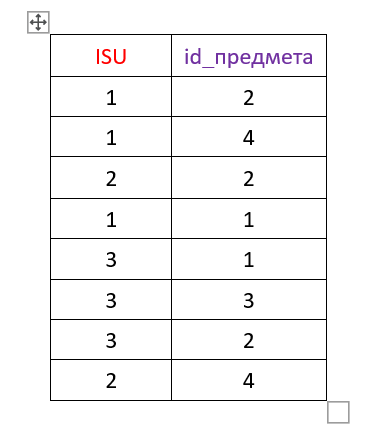
\includegraphics[width=0.7\textwidth]{pic/911.png}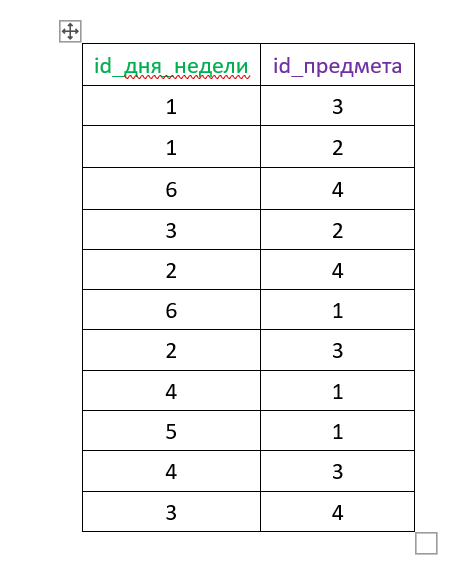
\includegraphics[width=0.7\textwidth]{pic/912.png} }
\end{minipage}
\end{figure}

В базе данных расписания ИТМО есть 2 таблицы:
\begin{itemize}
    \item В таблице 1 (рис. 1) каждому студенту по его номеру ИСУ сопоставлены предметы по их id. У одного номера ИСУ (студента) может быть много предметов, при этом на один предмет может ходить несколько студентов.
    \item В таблице 2 (рис. 2) каждому дню недели по его id (порядковый номер: 1-пн, 2-вт, 3-ср и т. д.) сопоставлены предметы по их id. В один день могут проводиться пары по нескольким предметам, при этом пары по одному предмету могут проходить несколько дней в неделе.
\end{itemize}
От Васи требуется по имеющимся данным вывести все возможные кортежи вида:

\begin{center}(номер ИСУ, день когда у этого студента есть пары)\end{center}

Например, ответ вида $\{(1, 1), (1, 5), (2, 1)\}$ будет означать что студент с ISU №1 имеет пары в понедельник и пятницу, а студент с ISU №2 имеет пары только в понедельник.

Помогите Васе решить данную задачу, используя ваши знания по дискретной математике.

---------------

Автор -- Тимур Гонтарь, М3206\question
Даны отношения $R_1$, $R_2$ и $R_3$ на множестве $A = \{1; 2; 3; 4; 5;\}$ 
\begin{enumerate}
	\renewcommand{\labelenumi}{\alph{enumi})}
	\item $R_1 = \{(1; 1); (2; 2); (3; 3); (2; 1);  (3; 1); (1; 3)\}$
	\item $R_2 = \{(1; 2); (2; 2); (3; 4); (3; 5); (4; 5)\}$
	\item $R_2 = \{(1; 3); (1; 5); (3; 4); (3; 5); (4; 5)\}$
\end{enumerate}

\begin{enumerate}
	\renewcommand{\labelenumi}{\alph{enumi})}
	\item $(R_1 \cap R_2) \cup R_3$
	\item $R_1 \cup R_3$
	\item $R_1^3 \cap R_3^-1$
	\item $R_3 \cup R_2^2$
	\item $R_2 \cup \overline{R_1}$
\end{enumerate}

определите основные свойства, получившихся отношений
определите какие свойства сохраняются относительно исходных отношений $R_1$, $R_2$ и $R_3$ 

\underline{примечание:} результатом может быть пустое множество

\end{questions}
\newpage
%%% begin test
\begin{flushright}
\begin{tabular}{p{2.8in} r l}
%\textbf{\class} & \textbf{ФИО:} & \makebox[2.5in]{\hrulefill}\\
\textbf{\class} & \textbf{ФИО:} &Дополнительный 9
\\

\textbf{\examdate} &&\\
%\textbf{Time Limit: \timelimit} & Teaching Assistant & \makebox[2in]{\hrulefill}
\end{tabular}\\
\end{flushright}
\rule[1ex]{\textwidth}{.1pt}


\begin{questions}
\question
В самом мирном городе мира, Лос-Сантосе, орудуют несколько бандитских группировок: Гроув-стрит, Баллос и Вагос. Некоторые районы города, для удобства бандитов помеченные цифрами \{0...9\}, находятся под влиянием этих банд:
\begin{itemize}
    \item Гроув-стрит: \{1, 2, 3, 7, 9\}
    \item Баллос: \{1, 3, 7, 8\}
    \item Вагос: \{4, 6, 7, 9\}
\end{itemize}
Районы, оказавшиеся под влиянием нескольких банд, называются спорными территориями.
\\
\\
В один прекрасный летний день Си-Джей увидел на стене своего дома граффити с сообщением от информатора из банды Баллосов. Для конспирации он оставил его в таком виде:
\begin{equation*}
B \cap \overline{G} \cup G \cap V \cap \overline{B} \cup G \cap B \cap \overline{V}
\end{equation*}
В нем содержатся номера районов, на которые полиция планирует совершить облаву. Вам, как самому умному представителю Гроув-Стрит, необходимо расшифровать граффити, а затем ответить на следующие вопросы:

\begin{itemize}
    \item Какие районы не под контролем ни одной из этих банд?
    \item Какое количество районов охватывают все три банды?
    \item На какие из районов, находящихся под вашим влиянием, будет совершена облава?
\end{itemize}

---------------

Автор -- Константин Васильев, М3213\question
Упростите следующее выражение с учетом того, что $A\subset B \subset C \subset D \subset U; A \neq \emptyset$
\begin{equation*}
	\overline{A} \cap \overline{C} \cap D \cup \overline{B} \cap \overline{C} \cap D \cup A \cap B
\end{equation*}

Примечание: $U$ -- универсум\question
Укажите номера множеств, являющихся подмножествами множества
\begin{equation*}
	Q = A \cap \bar{D} \cup B \cap C \cup \bar{A} \cap \bar{B} \cap D \cup A \cap C
\end{equation*}

\begin{enumerate}
	\renewcommand{\labelenumi}{\arabic{enumi})}
	\item $P = A \cap \bar{B} \cap D \cup \bar{A} \cap \bar{B} \cap C$;
	\item $P = A \cap B \cap D \cup \bar{A} \cap \bar{C} \cap D$;
	\item $P = B \cap \bar{C} \cap \bar{D} \cup A \cap B \cap \bar{C}$;
	\item $P = A \cap \bar{C} \cap \bar{D} \cup \bar{A} \cap \bar{B} \cap D$.
\end{enumerate}
\question
Постройте разбиения множеств:
\begin{enumerate}
	\renewcommand{\labelenumi}{\alph{enumi})}
	\item $A = \{6, 7, 8, 9, 11, 14, 34, 54, 47, 18, 91, 55, 65, 76, 28, 19\};$
	\item $B = \{0, 11, 14, 34, 22, 33, 44, 55, 65, 76, 28, 19\}$
	\item $A \cup B$
	\item $A \cap B$
\end{enumerate}
Таким образом, чтобы все разбиения имели как минимум 2 одинаковых множества в разбиениях.
Мощность каждого разбиение была более 5.
Докажите, что ваш ответ соответствует указанным условиям!
\question
Пусть у нас есть $P$ -- множество студентов города Санкт-Петербург, из них $A$ -- третьекурсники, $B$ -- проходят профессиональную переподготовку, а $C$ -- стажируются в Яндексе. Для статьи “Как учиться на третьем курсе университета ИТМО, проходить профессиональную подготовку и не умереть” Мегабайт создал выборку $D$.
\\
\\
Упростите множество $E = (P \cap D \cup C \cap \overline{B} \cap \overline{D} \cup B \cap A \cap \overline{C}) \cap \overline{C} \cap \overline{D} \cap P$, а затем опишите его словами.
\\
\\
---------------

Автор -- Антонина Чернова, М33081\question
Возьмём множество $M = \{1, 2, 3, 4, 5, 6, 7, 8, 9\}$. Определите свойства и виды бинарных отношений:
\begin{itemize}
    \item $xRy \Leftrightarrow x$ делит $y$
    \item $xRy \Leftrightarrow x + y = 8$
    \item $xRy \Leftrightarrow x + y \in M$
\end{itemize}
---------------

Автор -- Алексей Лёвушкин, М3204\question
Дана декартова система координат. Ось $x$ представляет собой множество $X$, ось $y$ - множество $Y$. На этих двух множествах определены бинарные отношения, которые схематически изображены в виде графиков выше (то есть, например, для графика с рис. 1 будет верно, что пары $(0, 0), (1, 1), (2, 2), (3, 3), (4, 4), (5, 5)$ входят в бинарное отношение, соответствующее графику). Для каждого из таких отношений определить:
\begin{itemize}
    \item Каким типом отношения соответствия оно является?
    \item Является ли оно функциональным отношением? Если да, то каким именно (сюръекция, инъекция, биекция)?
\end{itemize}
Обоснуйте своё решение. После этого, аналогично данным в условии графикам, придумайте отношение (любое), которое будет представлять собой полностью определенную функцию, и при этом будет инъективно и не сюръективно.
\\
\begin{figure}[h]

\begin{minipage}[h]{0.55\linewidth}
\end{minipage}
\begin{minipage}[h]{0.45\linewidth}
\center{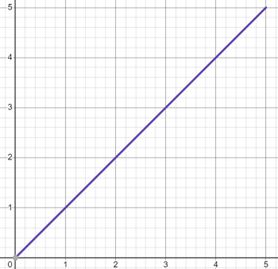
\includegraphics[width=0.7\textwidth]{pic/711.png}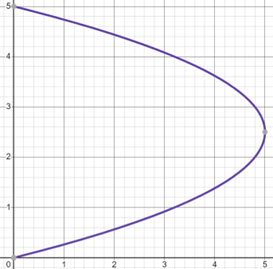
\includegraphics[width=0.7\textwidth]{pic/712.png}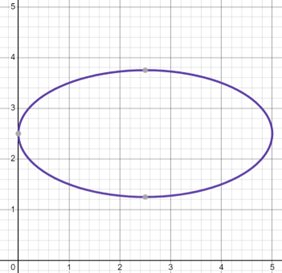
\includegraphics[width=0.7\textwidth]{pic/713.png} }
\end{minipage}
\end{figure}

---------------

Автор -- Тимур Гонтарь, М3206\question
Приведите  пример  нескольких бинарных отношений:
\begin{enumerate}
	\renewcommand{\labelenumi}{\alph{enumi})}
	\item отношение, которое является композиции нескольких бинарных отношений,  которое  нестрого порядка  и антисимметрично (укажите все бинарные отношения, участвующие в композиции)
	\item отношение, которое частично упорядочивает множество и как минимум 7 элементов упорядочены (обязательно покажите порядок элементов множества, полученный упордочиванием бинарным отношением)
	\item отношение, такое что обратное к нему  обладает одинаковыми с ним свойствами и оба антирефлексивны и симметричны (докажите, что свойства сохранаются)
\end{enumerate}

\underline{примечание:} важно показать  множества, на которых задано бинарное отношение и доказать, что ваше бинарное отношение обладает заданными свойствами
\question
В перерыве между парами дискретной математики вы с друзьями решили зарубиться в домино. Иллюстрация ниже визуализирует данный момент игры.

\\
\begin{figure}[h]

\begin{minipage}[h]{0.55\linewidth}
\end{minipage}
\begin{minipage}[h]{0.45\linewidth}
\center{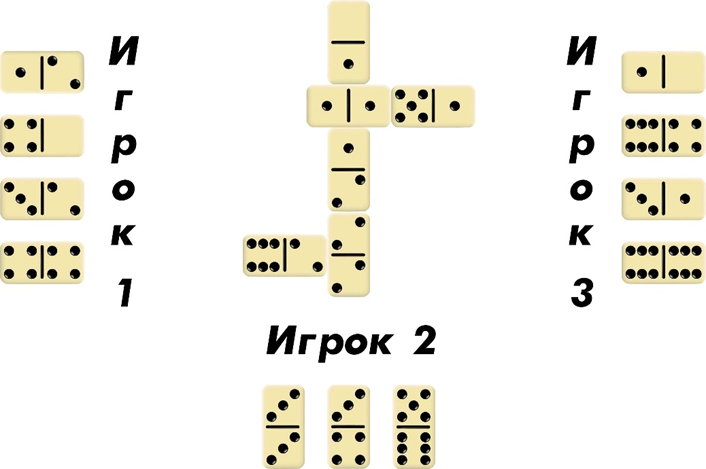
\includegraphics[width=0.7\textwidth]{pic/941.png} }
\end{minipage}
\end{figure}

Так как вы — умные студенты, вам стало интересно интерпретировать партию в виде бинарных отношений. Запишите отношения:
\begin{itemize}
    \item $G = \{(a,b)|a$ и $b$ – стороны свободных доминошек, лежащих на столе, где a – свободная сторона$\}$
    \item $R_1 = \{(a,b)|a$ и $b$ – стороны одной доминошки в руке у первого игрока$\}$
    \item $R_2 = \{(a,b)|a$ и $b$ – стороны одной доминошки в руке у второго игрока$\}$
    \item $R_3 = \{(a,b)|a$ и $b$ – стороны одной доминошки в руке у третьего игрока$\}$
\end{itemize}

Используя операцию композиции, составьте новые бинарные отношения:
\begin{itemize}
    \item $P_1$ – возможные ходы у первого игрока
    \item $P_2$ – возможные ходы у второго игрока
    \item $P_3$ – возможные ходы у третьего игрока
\end{itemize}


Ходом является пара крайних номеров стоящих рядом доминошек.
\\
---------------

Автор -- Константин Васильев, М3213\question
Даны отношения $R_1$, $R_2$ и $R_3$ на множестве $A = \{1; 2; 3; 4; 5;\}$ 
\begin{enumerate}
	\renewcommand{\labelenumi}{\alph{enumi})}
	\item $R_1 = \{(2; 1); (1; 2); (2; 3); (3; 2); (3; 1); (1; 3)\}$
	\item $R_2 = \{(1; 2); (2; 2); (1; 3); (1; 5); (2; 3); (2; 4); (2; 5); (4; 5)\}$
	\item $R_3 = \{(1; 2); (2; 2); (1; 3); (1; 5); (3; 4); (3; 5); (4; 5)\}$
\end{enumerate}

\begin{enumerate}
	\renewcommand{\labelenumi}{\alph{enumi})}
	\item $\overline{R_1} \cap R_2^{-1} \cap R_3$
	\item $(R_1^3 \cup R_2) \cap R_3^{-1}$
	\item $R_3 \cap R_3^{-1}$
	\item $R_3^{-1} \cup \overline{R_2^{-1}}$
	\item $R_1^{-1} \cup \overline{R_2} \cup R_3$
\end{enumerate}

определите основные свойства, получившихся отношений
определите какие свойства сохраняются относительно исходных отношений $R_1$, $R_2$ и $R_3$ 

\underline{примечание:} результатом может быть пустое множество

\end{questions}
\newpage
%%% begin test
\begin{flushright}
\begin{tabular}{p{2.8in} r l}
%\textbf{\class} & \textbf{ФИО:} & \makebox[2.5in]{\hrulefill}\\
\textbf{\class} & \textbf{ФИО:} &Дополнительный 10
\\

\textbf{\examdate} &&\\
%\textbf{Time Limit: \timelimit} & Teaching Assistant & \makebox[2in]{\hrulefill}
\end{tabular}\\
\end{flushright}
\rule[1ex]{\textwidth}{.1pt}


\begin{questions}
\question
Вы -- великая искательница сокровищ Лариса Крафтовое. Очередное путешествие забросило вас в подземные гробницы Сигизмунда I. К сожалению, на вашем пути встал очень назойливый мраморный привратник, который по всем канонам жанра имеет для вас пару загадок.
\\
\\
Привратник загадывает свое множество $X$, а также дает вам парочку других $(A,B,C…)$, объединяя, пересекая, дополняя и/или выполняя разность над которыми вы должны получить его множество. Загвоздка лишь в том, что привратник сам выбирает расстановку множеств в формуле, поэтому вам остается лишь вставить операции и расставить скобки (при надобности).

\paragraph{Загадка 1:}
\begin{equation*}
    X=\{2,3\}
\end{equation*}
\begin{equation*}
    A=\{1,2,3\}; B=\{3,4,5\}; C=\{1,4,5\}; D=\{2,3,5\}
    \end{equation*}
\begin{equation*}
    A ? B ? C ? D ? A ? C = X
\end{equation*}

\paragraph{Загадка 2:}
\begin{equation*}
    X=\{5,6\}
\end{equation*}
\begin{equation*}
    A=\{1,2,3,4\}; B=\{2,4,6\}; C=\{1,3,5\}
    \end{equation*}
\begin{equation*}
    A ? B ? C ? A = X
\end{equation*}

---------------

Автор -- Константин Васильев, М3213\question
Упростите следующее выражение с учетом того, что $A\subset B \subset C \subset D \subset U; A \neq \emptyset$
\begin{equation*}
	\overline{A} \cap \overline{B} \cup B \cap \overline{C} \cup \overline{C} \cap D
\end{equation*}

Примечание: $U$ -- универсум\question
Укажите номера множеств, являющихся подмножествами множества
\begin{equation*}
	Q = \bar{A} \cap C \cup A \cap \bar{B} \cup A \cap \bar{C} \cup \bar{A} \cap B \cap D
\end{equation*}

\begin{enumerate}
	\renewcommand{\labelenumi}{\arabic{enumi})}
	\item $P = B \cap C \cap D \cup \bar{A} \cap B \cap C$;
	\item $P = \bar{B} \cap \bar{C} \cap D \cup B \cap \bar{C} \cap \bar{D}$;
	\item $P = A \cap \bar{B} \cap D \cup A \cap C \cap D$;
	\item $P = \bar{B} \cap \bar{C} \cup \bar{A} \cap \bar{B} \cap D$.
\end{enumerate}
\question
Постройте разбиения множеств:
\begin{enumerate}
	\renewcommand{\labelenumi}{\alph{enumi})}
	\item $A = \{6, 7, 8, 9, 11, 14, 34, 54, 47, 18, 91, 55, 65, 76, 28, 19\};$
	\item $B = \{0, 11, 22, 33, 44, 55, 65, 76, 28, 19\}$
	\item $A \cup B$
\end{enumerate}
Таким образом, чтобы все разбиения имели как минимум 2 одинаковых множества в разбиениях.
Мощность каждого разбиение была более 3.
Докажите, что ваш ответ соответствует указанным условиям!
\question
Пусть у нас есть $P$ -- множество студентов города Санкт-Петербург, из них $A$ -- третьекурсники, $B$ -- проходят профессиональную переподготовку, а $C$ -- стажируются в Яндексе. Для статьи “Как учиться на третьем курсе университета ИТМО, проходить профессиональную подготовку и не умереть” Мегабайт создал выборку $D$.
\\
\\
Упростите множество $E = (P \cap D \cup C \cap \overline{B} \cap \overline{D} \cup B \cap A \cap \overline{C}) \cap \overline{C} \cap \overline{D} \cap P$, а затем опишите его словами.
\\
\\
---------------

Автор -- Антонина Чернова, М33081\question
Довольные студенты ИТМО сдали летнюю сессию и намерены поехать домой на некоторое время. К сожалению, чтобы добраться до пункта назначения, им потребуется сделать несколько пересадок.

Пусть множество всех населенных пунктов выглядит как: $A = \{1, 2, 3, 4, 5, 6\}$.
\\
Тогда $R = \{(1, 3), (3, 1), (2, 4), (4, 2), (1, 5), (5, 1), (2, 3), (3, 2)\}$ -- можно доехать на автобусе, $S = \{(5, 6), (6, 5), (3, 6), (6, 3)\}$ -- можно долететь на самолете.
\\
Какими свойствами обладают отношения R и S?
\\
---------------

Автор -- Елизавета Котельникова, М3212\question
Установите, является ли каждое из перечисленных ниже отношений на А ($R \subseteq A \times A$) отношением эквивалентности (обоснование ответа обязательно). Для каждого отношения эквивалентности постройте классы 
эквивалентности и постройте граф отношения:
\begin{enumerate}
	\renewcommand{\labelenumi}{\alph{enumi})}
	\item Пусть A -- множество имен. $A = \{ $Алексей, Иван, Петр, Александр, Павел, Андрей$ \}$. Тогда отношение $R$ верно на парах имен, начинающихся с одной и той же буквы, и только на них.
	\item $A = \{-10, -9, ..., 9, 10\}$ и отношение $ R = \{(a,b)|a^{2} = b^{2}\}$
	\item На множестве $A = \{1; 2; 3\}$ задано отношение $R = \{(1; 1); (2; 2); (3; 3); (3; 2); (1; 2); (2; 1)\}$
\end{enumerate}\question
Пусть имеется бинарное отношение $R$ на $ A \times A$. Докажите, что если $R$ -- одновременно и отношение эквивалентности и отношение частичного порядка, то оно -- отношение равенства.
\\
---------------

Автор -- Алексей Ващенков, М3205\question
Вася хочет устроиться бэкенд разработчиком в ИТМО, работать с ИСУ. На собеседовании тимлид дал ему тестовое задание, чтобы определить его уровень знаний:
\\
\begin{figure}[h]

\begin{minipage}[h]{0.55\linewidth}
\end{minipage}
\begin{minipage}[h]{0.45\linewidth}
\center{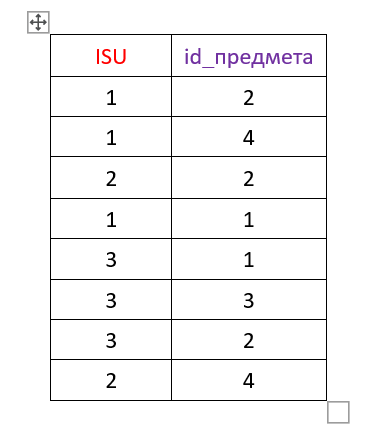
\includegraphics[width=0.7\textwidth]{pic/911.png}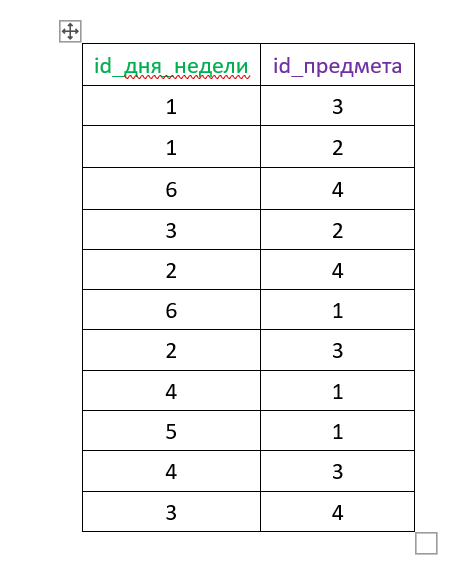
\includegraphics[width=0.7\textwidth]{pic/912.png} }
\end{minipage}
\end{figure}

В базе данных расписания ИТМО есть 2 таблицы:
\begin{itemize}
    \item В таблице 1 (рис. 1) каждому студенту по его номеру ИСУ сопоставлены предметы по их id. У одного номера ИСУ (студента) может быть много предметов, при этом на один предмет может ходить несколько студентов.
    \item В таблице 2 (рис. 2) каждому дню недели по его id (порядковый номер: 1-пн, 2-вт, 3-ср и т. д.) сопоставлены предметы по их id. В один день могут проводиться пары по нескольким предметам, при этом пары по одному предмету могут проходить несколько дней в неделе.
\end{itemize}
От Васи требуется по имеющимся данным вывести все возможные кортежи вида:

\begin{center}(номер ИСУ, день когда у этого студента есть пары)\end{center}

Например, ответ вида $\{(1, 1), (1, 5), (2, 1)\}$ будет означать что студент с ISU №1 имеет пары в понедельник и пятницу, а студент с ISU №2 имеет пары только в понедельник.

Помогите Васе решить данную задачу, используя ваши знания по дискретной математике.

---------------

Автор -- Тимур Гонтарь, М3206\question
Даны отношения $R_1$, $R_2$ и $R_3$ на множестве $A = \{1; 2; 3; 4; 5;\}$ 
\begin{enumerate}
	\renewcommand{\labelenumi}{\alph{enumi})}
	\item $R_1 = \{(1; 1); (2; 2); (3; 3); (2; 1);  (3; 1); (1; 3)\}$
	\item $R_2 = \{(1; 2); (2; 2); (3; 4); (3; 5); (4; 5)\}$
	\item $R_2 = \{(1; 3); (1; 5); (3; 4); (3; 5); (4; 5)\}$
\end{enumerate}

\begin{enumerate}
	\renewcommand{\labelenumi}{\alph{enumi})}
	\item $(R_1 \cap R_2) \cup R_3$
	\item $R_1 \cup R_3$
	\item $R_1^3 \cap R_3^-1$
	\item $R_3 \cup R_2^2$
	\item $R_2 \cup \overline{R_1}$
\end{enumerate}

определите основные свойства, получившихся отношений
определите какие свойства сохраняются относительно исходных отношений $R_1$, $R_2$ и $R_3$ 

\underline{примечание:} результатом может быть пустое множество

\end{questions}
\newpage
%%% begin test
\begin{flushright}
\begin{tabular}{p{2.8in} r l}
%\textbf{\class} & \textbf{ФИО:} & \makebox[2.5in]{\hrulefill}\\
\textbf{\class} & \textbf{ФИО:} &M3115
\\

\textbf{\examdate} &&\\
%\textbf{Time Limit: \timelimit} & Teaching Assistant & \makebox[2in]{\hrulefill}
\end{tabular}\\
\end{flushright}
\rule[1ex]{\textwidth}{.1pt}


\begin{questions}
\question
В самом мирном городе мира, Лос-Сантосе, орудуют несколько бандитских группировок: Гроув-стрит, Баллос и Вагос. Некоторые районы города, для удобства бандитов помеченные цифрами \{0...9\}, находятся под влиянием этих банд:
\begin{itemize}
    \item Гроув-стрит: \{1, 2, 3, 7, 9\}
    \item Баллос: \{1, 3, 7, 8\}
    \item Вагос: \{4, 6, 7, 9\}
\end{itemize}
Районы, оказавшиеся под влиянием нескольких банд, называются спорными территориями.
\\
\\
В один прекрасный летний день Си-Джей увидел на стене своего дома граффити с сообщением от информатора из банды Баллосов. Для конспирации он оставил его в таком виде:
\begin{equation*}
B \cap \overline{G} \cup G \cap V \cap \overline{B} \cup G \cap B \cap \overline{V}
\end{equation*}
В нем содержатся номера районов, на которые полиция планирует совершить облаву. Вам, как самому умному представителю Гроув-Стрит, необходимо расшифровать граффити, а затем ответить на следующие вопросы:

\begin{itemize}
    \item Какие районы не под контролем ни одной из этих банд?
    \item Какое количество районов охватывают все три банды?
    \item На какие из районов, находящихся под вашим влиянием, будет совершена облава?
\end{itemize}

---------------

Автор -- Константин Васильев, М3213\question
Упростите следующее выражение с учетом того, что $A\subset B \subset C \subset D \subset U; A \neq \emptyset$
\begin{equation*}
	A \cap C  \cap D \cup B \cap \overline{C} \cap D \cup B \cap C \cap D
\end{equation*}

Примечание: $U$ -- универсум\question
Укажите номера множеств, являющихся подмножествами множества
\begin{equation*}
	Q = A \cap \bar{D} \cup B \cap C \cup \bar{A} \cap \bar{B} \cap D \cup A \cap C
\end{equation*}

\begin{enumerate}
	\renewcommand{\labelenumi}{\arabic{enumi})}
	\item $P = B \cap C \cap D \cup \bar{A} \cap B \cap C$;
	\item $P = \bar{B} \cap \bar{C} \cap D \cup B \cap \bar{C} \cap \bar{D}$;
	\item $P = A \cap \bar{B} \cap D \cup A \cap C \cap D$;
	\item $P = \bar{B} \cap \bar{C} \cup \bar{A} \cap \bar{B} \cap D$.
\end{enumerate}
\question
Постройте разбиения множеств:
\begin{enumerate}
	\renewcommand{\labelenumi}{\alph{enumi})}
	\item $A = \{6, 7, 8, 9, 11, 14, 34, 91, 55, 65, 76, 28, 93, 94, \};$
	\item $B = \{8, 9, 11, 22, 33, 44, 55, 65, 67, 87, 91, 92, 93, 94, 95, 98\}$
	\item $A \cup B$
	\item $A \cap B$
\end{enumerate}
Таким образом, чтобы все разбиения имели как минимум 2 одинаковых множества в разбиениях.
Мощность каждого разбиение была более 4.
Докажите, что ваш ответ соответствует указанным условиям!\question
Упростить выражения, используя свойства операций над множествами:

\begin{enumerate}
	\renewcommand{\labelenumi}{\alph{enumi})}
	\item $(A \cap B \cap C \cap \bar{D}) \cup(\bar{A} \cap C) \cup(\bar{B} \cap C) \cup(C \cap D)$;
	\item $(\bar{A} \cup B \cup \bar{C}) \cap(A \cap \bar{B} \cap C) \cap \overline{(A \cup C)}$.
\end{enumerate}
\question
Возьмём множество $M = \{1, 2, 3, 4, 5, 6, 7, 8, 9\}$. Определите свойства и виды бинарных отношений:
\begin{itemize}
    \item $xRy \Leftrightarrow x$ делит $y$
    \item $xRy \Leftrightarrow x + y = 8$
    \item $xRy \Leftrightarrow x + y \in M$
\end{itemize}
---------------

Автор -- Алексей Лёвушкин, М3204\question
Установите, является ли каждое из перечисленных ниже отношений на А ($R \subseteq A \times A$) отношением эквивалентности (обоснование ответа обязательно). Для каждого отношения эквивалентности постройте классы 
эквивалентности и постройте граф отношения:
\begin{enumerate}
	\renewcommand{\labelenumi}{\alph{enumi})}
	\item $A = \{a, b, c, d, p, t\}$ задано отношение $R = \{(a, a), (b, b), (b, c), (b, d), (c, b), (c, c), (c, d), (d, b), (d, c), (d, d), (p,p), (t,t)\}$
	\item $A = \{-10, -9, ..., 9, 10\}$ и отношение $R = \{(a,b)|a^{3} = b^{3}\}$
	\item $F(x)=x^{2}+1$, где $x \in A = [-2, 4]$ и отношение $R = \{(a,b)|F(a) = F(b)\}$
\end{enumerate}\question
Приведите  пример  нескольких бинарных отношений:
\begin{enumerate}
	\renewcommand{\labelenumi}{\alph{enumi})}
	\item отношение, которое является композиции нескольких бинарных отношений,  которое  нестрого порядка и функционально (укажите все бинарные отношения, участвующие в композиции)
	\item отношение, которое частично упорядочивает множество и как минимум 6 элементов упорядочены (обязательно покажите порядок элементов множества, полученный упордочиванием бинарным отношением)
	\item отношение, такое что обратное к нему  обладает одинаковыми с ним свойствами и оба эквивалентны (докажите, что свойства сохранаются)
\end{enumerate}

\underline{примечание:} важно показать  множества, на которых задано бинарное отношение и доказать, что ваше бинарное отношение обладает заданными свойствами
\question
Вася хочет устроиться бэкенд разработчиком в ИТМО, работать с ИСУ. На собеседовании тимлид дал ему тестовое задание, чтобы определить его уровень знаний:
\\
\begin{figure}[h]

\begin{minipage}[h]{0.55\linewidth}
\end{minipage}
\begin{minipage}[h]{0.45\linewidth}
\center{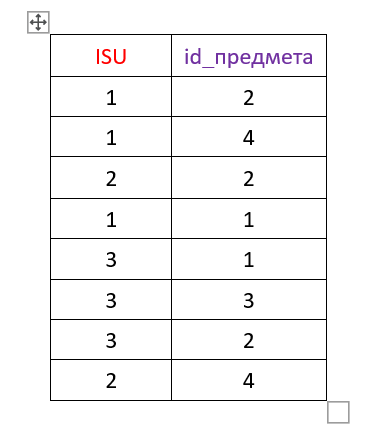
\includegraphics[width=0.7\textwidth]{pic/911.png}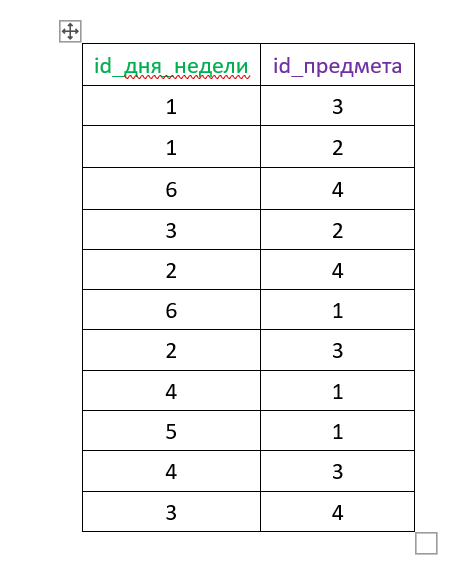
\includegraphics[width=0.7\textwidth]{pic/912.png} }
\end{minipage}
\end{figure}

В базе данных расписания ИТМО есть 2 таблицы:
\begin{itemize}
    \item В таблице 1 (рис. 1) каждому студенту по его номеру ИСУ сопоставлены предметы по их id. У одного номера ИСУ (студента) может быть много предметов, при этом на один предмет может ходить несколько студентов.
    \item В таблице 2 (рис. 2) каждому дню недели по его id (порядковый номер: 1-пн, 2-вт, 3-ср и т. д.) сопоставлены предметы по их id. В один день могут проводиться пары по нескольким предметам, при этом пары по одному предмету могут проходить несколько дней в неделе.
\end{itemize}
От Васи требуется по имеющимся данным вывести все возможные кортежи вида:

\begin{center}(номер ИСУ, день когда у этого студента есть пары)\end{center}

Например, ответ вида $\{(1, 1), (1, 5), (2, 1)\}$ будет означать что студент с ISU №1 имеет пары в понедельник и пятницу, а студент с ISU №2 имеет пары только в понедельник.

Помогите Васе решить данную задачу, используя ваши знания по дискретной математике.

---------------

Автор -- Тимур Гонтарь, М3206\question
Даны отношения $R_1$, $R_2$ и $R_3$ на множестве $A = \{1; 2; 3; 4; 5;\}$ 
\begin{enumerate}
	\renewcommand{\labelenumi}{\alph{enumi})}
	\item $R_1 = \{(2; 1); (1; 2); (2; 3); (3; 2); (3; 1); (1; 3)\}$
	\item $R_2 = \{(1; 2); (2; 2); (1; 3); (1; 5); (2; 3); (2; 4); (2; 5); (4; 5)\}$
	\item $R_3 = \{(1; 2); (2; 2); (1; 3); (1; 5); (3; 4); (3; 5); (4; 5)\}$
\end{enumerate}

\begin{enumerate}
	\renewcommand{\labelenumi}{\alph{enumi})}
	\item $\overline{R_1} \cap R_2^{-1} \cap R_3$
	\item $(R_1^3 \cup R_2) \cap R_3^{-1}$
	\item $R_3 \cap R_3^{-1}$
	\item $R_3^{-1} \cup \overline{R_2^{-1}}$
	\item $R_1^{-1} \cup \overline{R_2} \cup R_3$
\end{enumerate}

определите основные свойства, получившихся отношений
определите какие свойства сохраняются относительно исходных отношений $R_1$, $R_2$ и $R_3$ 

\underline{примечание:} результатом может быть пустое множество

\end{questions}
\newpage
%%% begin test
\begin{flushright}
\begin{tabular}{p{2.8in} r l}
%\textbf{\class} & \textbf{ФИО:} & \makebox[2.5in]{\hrulefill}\\
\textbf{\class} & \textbf{ФИО:} &Беттиуи Лина
\\

\textbf{\examdate} &&\\
%\textbf{Time Limit: \timelimit} & Teaching Assistant & \makebox[2in]{\hrulefill}
\end{tabular}\\
\end{flushright}
\rule[1ex]{\textwidth}{.1pt}


\begin{questions}
\question
Вы -- великая искательница сокровищ Лариса Крафтовое. Очередное путешествие забросило вас в подземные гробницы Сигизмунда I. К сожалению, на вашем пути встал очень назойливый мраморный привратник, который по всем канонам жанра имеет для вас пару загадок.
\\
\\
Привратник загадывает свое множество $X$, а также дает вам парочку других $(A,B,C…)$, объединяя, пересекая, дополняя и/или выполняя разность над которыми вы должны получить его множество. Загвоздка лишь в том, что привратник сам выбирает расстановку множеств в формуле, поэтому вам остается лишь вставить операции и расставить скобки (при надобности).

\paragraph{Загадка 1:}
\begin{equation*}
    X=\{1,2,5,6\}
\end{equation*}
\begin{equation*}
    A=\{1,2,3,4\}; B=\{2,3,4,5\}; C=\{2,5\}; D=\{4,5,6\}
    \end{equation*}
\begin{equation*}
    A ? B ? C ? D = X
\end{equation*}

\paragraph{Загадка 2:}
\begin{equation*}
    X=\{3,4,5\}
\end{equation*}
\begin{equation*}
    A=\{2,3,4,5\}; B=\{1,2,3\}; C=\{3,4,5\}; D=\{1,5,6\}
    \end{equation*}
\begin{equation*}
    A ? B ? C ? D = X
\end{equation*}

---------------

Автор -- Константин Васильев, М3213\question
Упростите следующее выражение с учетом того, что $A\subset B \subset C \subset D \subset U; A \neq \emptyset$
\begin{equation*}
	A \cap B  \cap \overline{C} \cup \overline{C} \cap D \cup B \cap C \cap D
\end{equation*}

Примечание: $U$ -- универсум\question
Укажите номера множеств, являющихся подмножествами множества
\begin{equation*}
	Q = \bar{A} \cup B \cap C \cup \bar{C} \cap \bar{D}
\end{equation*}

\begin{enumerate}
	\renewcommand{\labelenumi}{\arabic{enumi})}
	\item $P = B \cap C \cap D \cup \bar{A} \cap B \cap C$;
	\item $P = \bar{B} \cap \bar{C} \cap D \cup B \cap \bar{C} \cap \bar{D}$;
	\item $P = A \cap \bar{B} \cap D \cup A \cap C \cap D$;
	\item $P = \bar{B} \cap \bar{C} \cup \bar{A} \cap \bar{B} \cap D$.
\end{enumerate}
\question
Постройте разбиения множеств:
\begin{enumerate}
	\renewcommand{\labelenumi}{\alph{enumi})}
	\item $A = \{6, 7, 8, 9, 11, 14, 34, 54, 47, 18, 91, 55, 65, 76, 28, 19\};$
	\item $B = \{0, 11, 14, 34, 22, 33, 44, 55, 65, 76, 28, 19\}$
	\item $A \cup B$
	\item $A \cap B$
\end{enumerate}
Таким образом, чтобы все разбиения имели как минимум 2 одинаковых множества в разбиениях.
Мощность каждого разбиение была более 5.
Докажите, что ваш ответ соответствует указанным условиям!
\question
Докажите, что два выражения равны.

\begin{equation}
    (A \cup B) \backslash C = (A \backslash C) \cup (B \backslash C)
\end{equation}

\begin{equation}
    (A \backslash B) \cap C = (A \cap C) \backslash (B \cap C)
\end{equation}

\begin{equation}
    A \times (B \cap C) = (A \times B) \cap (A \times C)
\end{equation}

\begin{equation}
    A \times (B \cup C) = (A \times B) \cup (A \times C)
\end{equation}
\\
\\
$\times$ -- декартово произведение
\\
---------------

Автор -- Алексей Лёвушкин, М3204\question
Определить и обосновать, являются ли рефлексивными/симметричными/транзитивными, отношениями порядка, одно-однозначными/одно-многозначными/много-однозначными/много-многозначными бинарные отношения:
\begin{itemize}
    \item $aRb \Leftrightarrow a$ является ребёнком $b$ ($a$ и $b$ -- люди)
    \item $aRb \Leftrightarrow a$ и $b$ живут в одной стране ($a$ и $b$ -- люди)
    \item $aRb \Leftrightarrow a$ охотится на $b$ ($a$ и $b$ -- животные)
\end{itemize}
\\
Выделите среди этих БО отношения эквивалентности и разбейте их на классы эквивалентности, продемонстрировав алгоритм разбиения.
\\
---------------

Автор -- Алексей Лёвушкин, М3204\question
Установите, является ли каждое из перечисленных ниже отношений на А ($R \subseteq A \times A$) отношением эквивалентности (обоснование ответа обязательно). Для каждого отношения эквивалентности постройте классы 
эквивалентности и постройте граф отношения:
\begin{enumerate}
	\renewcommand{\labelenumi}{\alph{enumi})}
	\item А -- множество целых чисел и отношение $R = \{(a,b)|a + b = 5\}$
	\item Пусть A – множество имен. $A = \{ $Алексей, Иван, Петр, Александр, Павел, Андрей$ \}$. Тогда отношение $R $ верно на парах имен, начинающихся с одной и той же буквы, и только на них.
	\item На множестве $A = \{1; 2; 3; 4; 5\}$ задано отношение $R = \{(1; 2); (1; 3); (1; 5); (2; 3); (2; 4); (2; 5); (3; 4); (3; 5); (4; 5)\}$
\end{enumerate}\question
Приведите  пример  нескольких бинарных отношений:
\begin{enumerate}
	\renewcommand{\labelenumi}{\alph{enumi})}
	\item отношение, которое является композиции нескольких бинарных отношений,  которое  нестрого порядка и функционально (укажите все бинарные отношения, участвующие в композиции)
	\item отношение, которое частично упорядочивает множество и как минимум 6 элементов упорядочены (обязательно покажите порядок элементов множества, полученный упордочиванием бинарным отношением)
	\item отношение, такое что обратное к нему  обладает одинаковыми с ним свойствами и оба эквивалентны (докажите, что свойства сохранаются)
\end{enumerate}

\underline{примечание:} важно показать  множества, на которых задано бинарное отношение и доказать, что ваше бинарное отношение обладает заданными свойствами
\question
Петя решил поучаствовать в конкурсе рисунков, к сожалению, проблема была в том, что он совершенно не умел рисовать, но Петя был умным мальчиком, который знал бинарные отношения.
\\На декартовом произведении множества $A = \{-2, -1, 0, 1, 2, 3, 4, 5, 6, 7, 8, 9, 10, 11\}$ заданы бинарные отношения:
\begin{equation*}
R_1 = {(0, -2), (2, 0), (6, -2), (8, 0), (9, -2), (12, -2), (11, -1), (11, 1), (12, 2), (9, 2), (8, 0), (6, 2), (5, 5), (0, 5), (6, 7), (0, 6)}
\end{equation*}
\begin{center}и\end{center}
\begin{equation*}
R_2 = \{(10, -1), (10, -1), (9, 0)\}
\end{equation*}
Помогите Пете выиграть в конкурсе! Постройте композиции отношений $R_1^{-1}, R_2^{-1}$ и изобразите полученный результат на декартовой системе координат (задание можно дополнять другими композициями).
\\
---------------

Автор -- Анастасия Стеценко, М3207\question
Даны отношения $R_1$, $R_2$ и $R_3$ на множестве $A = \{1; 2; 3; 4; 5;\}$ 
\begin{enumerate}
	\renewcommand{\labelenumi}{\alph{enumi})}
	\item $R_1 = \{(3; 2); (3; 1); (1; 3)\}$
	\item $R_2 = \{(1; 2); (2; 2); (1; 3); (1; 5); (2; 3); (4; 5)\}$
	\item $R_2 = \{(1; 2); (2; 2); (3; 4); (3; 5); (4; 5)\}$
\end{enumerate}

\begin{enumerate}
	\renewcommand{\labelenumi}{\alph{enumi})}
	\item $R_1 \cap R_2$
	\item $(R_1 \cup R_2) \cap R_3$
	\item $R_3^2 \cap R_3^{-1}$
	\item $R_3 \cup \overline{R_2^2}$
	\item $R_1 \cup \overline{R_2} \cup R_3$
\end{enumerate}

определите основные свойства, получившихся отношений
определите какие свойства сохраняются относительно исходных отношений $R_1$, $R_2$ и $R_3$ 

\underline{примечание:} результатом может быть пустое множество

\end{questions}
\newpage
%%% begin test
\begin{flushright}
\begin{tabular}{p{2.8in} r l}
%\textbf{\class} & \textbf{ФИО:} & \makebox[2.5in]{\hrulefill}\\
\textbf{\class} & \textbf{ФИО:} &Богачёв Ростислав Олегович
\\

\textbf{\examdate} &&\\
%\textbf{Time Limit: \timelimit} & Teaching Assistant & \makebox[2in]{\hrulefill}
\end{tabular}\\
\end{flushright}
\rule[1ex]{\textwidth}{.1pt}


\begin{questions}
\question
Ребята приехали в математический лагерь, где каждый получил футболку с уникальным номером от 1 до 23. Отправившись на очередной полдник, они обнаружили, что нет ни одного кекса – их украли! Ребята сразу приступили к расследованию. Таким образом, они сделали вывод, что виновник – не один человек, а целая группа! У них получилось разделить всех ребят на 4 группы подозреваемых, в зависимости от того, кто где был в предположительное время совершения преступления по словам очевидцев.
\\(Легенда: С – столовая, D – двор, B – баскетбольная площадка, А - аллея): 
\begin{center}
$A: \{1, 2, 3, 21, 23, 5, 22, 18, 19, 6\}$
\\
$B: \{6, 22, 10, 15, 11, 13, 7, 18, 14, 9\}$
\\
$C: \{7, 8, 14, 20, 12, 4, 1, 2, 19, 6\}$
\\
$D: \{9, 13, 16, 17, 18, 19, 22, 14, 5, 6\}$
\end{center}
Так как ребята были отличными математиками, у них получилось составить выражение, которое раскроет, кто виноват в преступлении. 
\begin{equation*}
    A \cup B \cap \overline{C} \cup (A \cap D \cup \overline{C}) \cup D
\end{equation*}
Помогите им найти виновных.

---------------

Автор -- Баженова Мария, М3219\question
Упростите следующее выражение с учетом того, что $A\subset B \subset C \subset D \subset U; A \neq \emptyset$
\begin{equation*}
	\overline{B} \cap \overline{C} \cap D \cup \overline{A} \cap \overline{C} \cap D \cup \overline{A} \cap B
\end{equation*}

Примечание: $U$ -- универсум\question
Укажите номера множеств, являющихся подмножествами множества
\begin{equation*}
	Q = \bar{A} \cap B \cup A \cap \bar{B} \cup A \cap \bar{C} \cup \bar{A} \cap C \cap \bar{D}
\end{equation*}

\begin{enumerate}
	\renewcommand{\labelenumi}{\arabic{enumi})}
	\item $P = B \cap C \cap D \cup \bar{A} \cap B \cap C$;
	\item $P = \bar{B} \cap \bar{C} \cap D \cup B \cap \bar{C} \cap \bar{D}$;
	\item $P = A \cap \bar{B} \cap D \cup A \cap C \cap D$;
	\item $P = \bar{B} \cap \bar{C} \cup \bar{A} \cap \bar{B} \cap D$.
\end{enumerate}
\question
Постройте разбиения множеств:
\begin{enumerate}
	\renewcommand{\labelenumi}{\alph{enumi})}
	\item $A = \{6, 7, 8, 9, 11, 14, 34, 91, 55, 65, 76, 28, 19\};$
	\item $B = \{0, 1, 2, 3, 4, 8, 9, 11, 22, 33, 44, 55, 65, 76, 28, 19\}$
	\item $A \cup B$
	\item $A \cap B$
\end{enumerate}
Таким образом, чтобы все разбиения имели как минимум 2 одинаковых множества в разбиениях.
Мощность каждого разбиение была более 4.
Докажите, что ваш ответ соответствует указанным условиям!\question
Упростить выражения, используя свойства операций над множествами:

\begin{enumerate}
	\renewcommand{\labelenumi}{\alph{enumi})}
	\item $(A \cap B \cap C \cap \bar{D}) \cup(\bar{A} \cap C) \cup(\bar{B} \cap C) \cup(C \cap D)$;
	\item $(\bar{A} \cup B \cup \bar{C}) \cap(A \cap \bar{B} \cap C) \cap \overline{(A \cup C)}$.
\end{enumerate}
\question
Дано отношение на множестве $\{1, 2, 3, 4, 5\}$ 
\begin{equation*}
	aRb \iff a \leqslant b
\end{equation*}

(ЧАСТЬ 1) Какими основным свойствами обладает отношение? (Дайте обоснованный ответ по всем пунктам ниже: докажите наличие или отсутствие свойств)  
\begin{enumerate}
	\renewcommand{\labelenumi}{\alph{enumi})}
	\item рефлексивность / антирефлексивность / нерефлексивность
	\item симметричность / антисимметричность / асимметричность / несимметричность
	\item транзитивность / антитранзитивность / нетранзитивность
\end{enumerate}

(ЧАСТЬ 2) Обоснуйте свой ответ по каждому из приведенных ниже вопросов:
\begin{enumerate}
	\renewcommand{\labelenumi}{\alph{enumi})}
    \item Является ли это отношение отношением эквивалентности?
    \item Является ли это отношение функциональным?
    \item Каким из отношений соответствия (одно-многозначным, много-многозначный и т.д.) оно является?
    \item К каким из отношений порядка (строгого, не строгого и т.д.) можно отнести данное отношение?
\end{enumerate}
\question
Дана декартова система координат. Ось $x$ представляет собой множество $X$, ось $y$ - множество $Y$. На этих двух множествах определены бинарные отношения, которые схематически изображены в виде графиков выше (то есть, например, для графика с рис. 1 будет верно, что пары $(0, 0), (1, 1), (2, 2), (3, 3), (4, 4), (5, 5)$ входят в бинарное отношение, соответствующее графику). Для каждого из таких отношений определить:
\begin{itemize}
    \item Каким типом отношения соответствия оно является?
    \item Является ли оно функциональным отношением? Если да, то каким именно (сюръекция, инъекция, биекция)?
\end{itemize}
Обоснуйте своё решение. После этого, аналогично данным в условии графикам, придумайте отношение (любое), которое будет представлять собой полностью определенную функцию, и при этом будет инъективно и не сюръективно.
\\
\begin{figure}[h]

\begin{minipage}[h]{0.55\linewidth}
\end{minipage}
\begin{minipage}[h]{0.45\linewidth}
\center{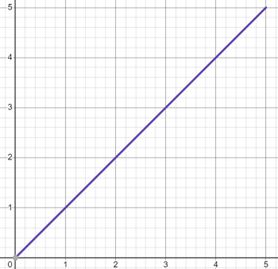
\includegraphics[width=0.7\textwidth]{pic/711.png}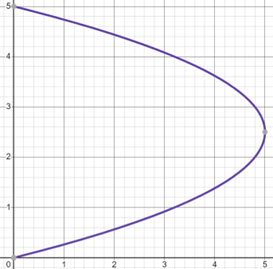
\includegraphics[width=0.7\textwidth]{pic/712.png}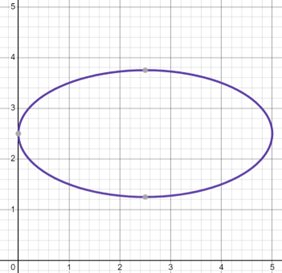
\includegraphics[width=0.7\textwidth]{pic/713.png} }
\end{minipage}
\end{figure}

---------------

Автор -- Тимур Гонтарь, М3206\question
Приведите  пример  нескольких бинарных отношений:
\begin{enumerate}
	\renewcommand{\labelenumi}{\alph{enumi})}
	\item отношение, которое является композиции нескольких бинарных отношений,  которое  нестрого порядка  и антисимметрично (укажите все бинарные отношения, участвующие в композиции)
	\item отношение, которое частично упорядочивает множество и как минимум 7 элементов упорядочены (обязательно покажите порядок элементов множества, полученный упордочиванием бинарным отношением)
	\item отношение, такое что обратное к нему  обладает одинаковыми с ним свойствами и оба антирефлексивны и симметричны (докажите, что свойства сохранаются)
\end{enumerate}

\underline{примечание:} важно показать  множества, на которых задано бинарное отношение и доказать, что ваше бинарное отношение обладает заданными свойствами
\question
Петя решил поучаствовать в конкурсе рисунков, к сожалению, проблема была в том, что он совершенно не умел рисовать, но Петя был умным мальчиком, который знал бинарные отношения.
\\На декартовом произведении множества $A = \{-2, -1, 0, 1, 2, 3, 4, 5, 6, 7, 8, 9, 10, 11\}$ заданы бинарные отношения:
\begin{equation*}
R_1 = {(0, -2), (2, 0), (6, -2), (8, 0), (9, -2), (12, -2), (11, -1), (11, 1), (12, 2), (9, 2), (8, 0), (6, 2), (5, 5), (0, 5), (6, 7), (0, 6)}
\end{equation*}
\begin{center}и\end{center}
\begin{equation*}
R_2 = \{(10, -1), (10, -1), (9, 0)\}
\end{equation*}
Помогите Пете выиграть в конкурсе! Постройте композиции отношений $R_1^{-1}, R_2^{-1}$ и изобразите полученный результат на декартовой системе координат (задание можно дополнять другими композициями).
\\
---------------

Автор -- Анастасия Стеценко, М3207\question
Даны отношения $R_1$, $R_2$ и $R_3$ на множестве $A = \{1; 2; 3; 4; 5;\}$ 
\begin{enumerate}
	\renewcommand{\labelenumi}{\alph{enumi})}
	\item $R_1 = \{(3; 2); (3; 1); (1; 3)\}$
	\item $R_2 = \{(1; 2); (2; 2); (1; 3); (4; 5)\}$
	\item $R_3 = \{(1; 2); (2; 2); (3; 4); (3; 5); (4; 5)\}$
\end{enumerate}

\begin{enumerate}
	\renewcommand{\labelenumi}{\alph{enumi})}
	\item $R_1 \cap R_2^{-1} \cup R_3^2$
	\item $(R_1 \cup R_2) \cap R_3$
	\item $R_3^2 \cap R_3^{-1}$
	\item $R_3^{-1} \cup \overline{R_2^{-1}}$
	\item $R_1^{-1} \cup \overline{R_2} \cup R_3$
\end{enumerate}

определите основные свойства, получившихся отношений
определите какие свойства сохраняются относительно исходных отношений $R_1$, $R_2$ и $R_3$ 

\underline{примечание:} результатом может быть пустое множество

\end{questions}
\newpage
%%% begin test
\begin{flushright}
\begin{tabular}{p{2.8in} r l}
%\textbf{\class} & \textbf{ФИО:} & \makebox[2.5in]{\hrulefill}\\
\textbf{\class} & \textbf{ФИО:} &Виноградов Дмитрий Евгеньич
\\

\textbf{\examdate} &&\\
%\textbf{Time Limit: \timelimit} & Teaching Assistant & \makebox[2in]{\hrulefill}
\end{tabular}\\
\end{flushright}
\rule[1ex]{\textwidth}{.1pt}


\begin{questions}
\question
В самом мирном городе мира, Лос-Сантосе, орудуют несколько бандитских группировок: Гроув-стрит, Баллос и Вагос. Некоторые районы города, для удобства бандитов помеченные цифрами \{0...9\}, находятся под влиянием этих банд:
\begin{itemize}
    \item Гроув-стрит: \{1, 2, 3, 7, 9\}
    \item Баллос: \{1, 3, 7, 8\}
    \item Вагос: \{4, 6, 7, 9\}
\end{itemize}
Районы, оказавшиеся под влиянием нескольких банд, называются спорными территориями.
\\
\\
В один прекрасный летний день Си-Джей увидел на стене своего дома граффити с сообщением от информатора из банды Баллосов. Для конспирации он оставил его в таком виде:
\begin{equation*}
B \cap \overline{G} \cup G \cap V \cap \overline{B} \cup G \cap B \cap \overline{V}
\end{equation*}
В нем содержатся номера районов, на которые полиция планирует совершить облаву. Вам, как самому умному представителю Гроув-Стрит, необходимо расшифровать граффити, а затем ответить на следующие вопросы:

\begin{itemize}
    \item Какие районы не под контролем ни одной из этих банд?
    \item Какое количество районов охватывают все три банды?
    \item На какие из районов, находящихся под вашим влиянием, будет совершена облава?
\end{itemize}

---------------

Автор -- Константин Васильев, М3213\question
Упростите следующее выражение с учетом того, что $A\subset B \subset C \subset D \subset U; A \neq \emptyset$
\begin{equation*}
	\overline{B} \cap \overline{C} \cap D \cup \overline{A} \cap \overline{C} \cap D \cup \overline{A} \cap B
\end{equation*}

Примечание: $U$ -- универсум\question
Укажите номера множеств, являющихся подмножествами множества
\begin{equation*}
	Q = \bar{A} \cap C \cup A \cap \bar{B} \cup A \cap \bar{C} \cup \bar{A} \cap B \cap D
\end{equation*}

\begin{enumerate}
	\renewcommand{\labelenumi}{\arabic{enumi})}
	\item $P = B \cap C \cap D \cup \bar{A} \cap B \cap C$;
	\item $P = \bar{B} \cap \bar{C} \cap D \cup B \cap \bar{C} \cap \bar{D}$;
	\item $P = A \cap \bar{B} \cap D \cup A \cap C \cap D$;
	\item $P = \bar{B} \cap \bar{C} \cup \bar{A} \cap \bar{B} \cap D$.
\end{enumerate}
\question
Постройте разбиения множеств:
\begin{enumerate}
	\renewcommand{\labelenumi}{\alph{enumi})}
	\item $A = \{6, 7, 8, 9, 11, 14, 34, 54, 47, 18, 91\};$
	\item $B = \{0, 1, 2, 3, 4, 5, 6, 7, 8, 9\}$
	\item $A \cap B$
\end{enumerate}
Таким образом, чтобы все разбиения имели как минимум 2 одинаковых множества в разбиениях.
Мощность каждого разбиение была более 3.
Докажите, что ваш ответ соответствует указанным условиям!\question
Пусть у нас есть $P$ -- множество студентов города Санкт-Петербург, из них $A$ -- третьекурсники, $B$ -- проходят профессиональную переподготовку, а $C$ -- стажируются в Яндексе. Для статьи “Как учиться на третьем курсе университета ИТМО, проходить профессиональную подготовку и не умереть” Мегабайт создал выборку $D$.
\\
\\
Упростите множество $E = (P \cap D \cup C \cap \overline{B} \cap \overline{D} \cup B \cap A \cap \overline{C}) \cap \overline{C} \cap \overline{D} \cap P$, а затем опишите его словами.
\\
\\
---------------

Автор -- Антонина Чернова, М33081\question
Дано отношение на множестве $\{1, 2, 3, 4, 5\}$ 
\begin{equation*}
	aRb \iff a \leqslant b
\end{equation*}

(ЧАСТЬ 1) Какими основным свойствами обладает отношение? (Дайте обоснованный ответ по всем пунктам ниже: докажите наличие или отсутствие свойств)  
\begin{enumerate}
	\renewcommand{\labelenumi}{\alph{enumi})}
	\item рефлексивность / антирефлексивность / нерефлексивность
	\item симметричность / антисимметричность / асимметричность / несимметричность
	\item транзитивность / антитранзитивность / нетранзитивность
\end{enumerate}

(ЧАСТЬ 2) Обоснуйте свой ответ по каждому из приведенных ниже вопросов:
\begin{enumerate}
	\renewcommand{\labelenumi}{\alph{enumi})}
    \item Является ли это отношение отношением эквивалентности?
    \item Является ли это отношение функциональным?
    \item Каким из отношений соответствия (одно-многозначным, много-многозначный и т.д.) оно является?
    \item К каким из отношений порядка (строгого, не строгого и т.д.) можно отнести данное отношение?
\end{enumerate}
\question
Установите, является ли каждое из перечисленных ниже отношений на А ($R \subseteq A \times A$) отношением эквивалентности (обоснование ответа обязательно). Для каждого отношения эквивалентности постройте классы 
эквивалентности и постройте граф отношения:
\begin{enumerate}
	\renewcommand{\labelenumi}{\alph{enumi})}
	\item $A = \{a, b, c, d, p, t\}$ задано отношение $R = \{(a, a), (b, b), (b, c), (b, d), (c, b), (c, c), (c, d), (d, b), (d, c), (d, d), (p,p), (t,t)\}$
	\item $A = \{-10, -9, ..., 9, 10\}$ и отношение $R = \{(a,b)|a^{3} = b^{3}\}$
	\item $F(x)=x^{2}+1$, где $x \in A = [-2, 4]$ и отношение $R = \{(a,b)|F(a) = F(b)\}$
\end{enumerate}\question
Приведите  пример  нескольких бинарных отношений:
\begin{enumerate}
	\renewcommand{\labelenumi}{\alph{enumi})}
	\item отношение, которое является композиции нескольких бинарных отношений,  которое  нестрого порядка  и антисимметрично (укажите все бинарные отношения, участвующие в композиции)
	\item отношение, которое частично упорядочивает множество и как минимум 7 элементов упорядочены (обязательно покажите порядок элементов множества, полученный упордочиванием бинарным отношением)
	\item отношение, такое что обратное к нему  обладает одинаковыми с ним свойствами и оба антирефлексивны и симметричны (докажите, что свойства сохранаются)
\end{enumerate}

\underline{примечание:} важно показать  множества, на которых задано бинарное отношение и доказать, что ваше бинарное отношение обладает заданными свойствами
\question
Даны отношения $R_1$ и $R_2$ на множестве $A = \{1; 2; 3; 4; 5\}$, постройте композиции отношений $R_1*R_2$, $R_2*R_1$,  $R_1*R_2^{-1}$, $R_1^{-1}*R_2$, $R_1^2$, $R_2^2$:
\begin{enumerate}
	\renewcommand{\labelenumi}{\alph{enumi})}
	\item $R_1 = \{(1; 1); (2; 2); (3; 3); (2; 1); (1; 2); (2; 3); (3; 2); (4; 1); (4; 5); (5; 4); (5; 5)\}$
	\item $R_2 = \{(1; 3); (2; 4); (5; 4); (1; 5); (4; 2); (2; 5)\}$
	\item задайте получившиеся отношения с помощью матриц, графов и перечислений 
	\item определите основные свойства, получившихся отношений
\end{enumerate}

\underline{примечание:} результатом может быть пустое множество
\question
Даны отношения $R_1$, $R_2$ и $R_3$ на множестве $A = \{1; 2; 3; 4; 5;\}$ 
\begin{enumerate}
	\renewcommand{\labelenumi}{\alph{enumi})}
	\item $R_1 = \{(3; 2); (3; 1); (1; 3)\}$
	\item $R_2 = \{(1; 2); (2; 2); (1; 3); (1; 5); (2; 3); (4; 5)\}$
	\item $R_2 = \{(1; 2); (2; 2); (3; 4); (3; 5); (4; 5)\}$
\end{enumerate}

\begin{enumerate}
	\renewcommand{\labelenumi}{\alph{enumi})}
	\item $R_1 \cap R_2$
	\item $(R_1 \cup R_2) \cap R_3$
	\item $R_3^2 \cap R_3^{-1}$
	\item $R_3 \cup \overline{R_2^2}$
	\item $R_1 \cup \overline{R_2} \cup R_3$
\end{enumerate}

определите основные свойства, получившихся отношений
определите какие свойства сохраняются относительно исходных отношений $R_1$, $R_2$ и $R_3$ 

\underline{примечание:} результатом может быть пустое множество

\end{questions}
\newpage
%%% begin test
\begin{flushright}
\begin{tabular}{p{2.8in} r l}
%\textbf{\class} & \textbf{ФИО:} & \makebox[2.5in]{\hrulefill}\\
\textbf{\class} & \textbf{ФИО:} &Войтович Дарья Александровна
\\

\textbf{\examdate} &&\\
%\textbf{Time Limit: \timelimit} & Teaching Assistant & \makebox[2in]{\hrulefill}
\end{tabular}\\
\end{flushright}
\rule[1ex]{\textwidth}{.1pt}


\begin{questions}
\question
Вы -- великая искательница сокровищ Лариса Крафтовое. Очередное путешествие забросило вас в подземные гробницы Сигизмунда I. К сожалению, на вашем пути встал очень назойливый мраморный привратник, который по всем канонам жанра имеет для вас пару загадок.
\\
\\
Привратник загадывает свое множество $X$, а также дает вам парочку других $(A,B,C…)$, объединяя, пересекая, дополняя и/или выполняя разность над которыми вы должны получить его множество. Загвоздка лишь в том, что привратник сам выбирает расстановку множеств в формуле, поэтому вам остается лишь вставить операции и расставить скобки (при надобности).

\paragraph{Загадка 1:}
\begin{equation*}
    X=\{1,2,5,6\}
\end{equation*}
\begin{equation*}
    A=\{1,2,3,4\}; B=\{2,3,4,5\}; C=\{2,5\}; D=\{4,5,6\}
    \end{equation*}
\begin{equation*}
    A ? B ? C ? D = X
\end{equation*}

\paragraph{Загадка 2:}
\begin{equation*}
    X=\{3,4,5\}
\end{equation*}
\begin{equation*}
    A=\{2,3,4,5\}; B=\{1,2,3\}; C=\{3,4,5\}; D=\{1,5,6\}
    \end{equation*}
\begin{equation*}
    A ? B ? C ? D = X
\end{equation*}

---------------

Автор -- Константин Васильев, М3213\question
Упростите следующее выражение с учетом того, что $A\subset B \subset C \subset D \subset U; A \neq \emptyset$
\begin{equation*}
	A \cap B  \cap \overline{C} \cup \overline{C} \cap D \cup B \cap C \cap D
\end{equation*}

Примечание: $U$ -- универсум\question
Укажите номера множеств, являющихся подмножествами множества
\begin{equation*}
	Q = \bar{A} \cap C \cup A \cap \bar{B} \cup A \cap \bar{C} \cup \bar{A} \cap B \cap D
\end{equation*}

\begin{enumerate}
	\renewcommand{\labelenumi}{\arabic{enumi})}
	\item $P = B \cap C \cap D \cup \bar{A} \cap B \cap C$;
	\item $P = \bar{B} \cap \bar{C} \cap D \cup B \cap \bar{C} \cap \bar{D}$;
	\item $P = A \cap \bar{B} \cap D \cup A \cap C \cap D$;
	\item $P = \bar{B} \cap \bar{C} \cup \bar{A} \cap \bar{B} \cap D$.
\end{enumerate}
\question
Постройте разбиения множеств:
\begin{enumerate}
	\renewcommand{\labelenumi}{\alph{enumi})}
	\item $A = \{6, 7, 8, 9, 11, 14, 34, 54, 47, 18, 91, 55, 65, 76, 28, 19\};$
	\item $B = \{0, 11, 22, 33, 44, 55, 65, 76, 28, 19\}$
	\item $A \cup B$
\end{enumerate}
Таким образом, чтобы все разбиения имели как минимум 2 одинаковых множества в разбиениях.
Мощность каждого разбиение была более 3.
Докажите, что ваш ответ соответствует указанным условиям!
\question
Упростить выражения, используя свойства операций над множествами:

\begin{enumerate}
	\renewcommand{\labelenumi}{\alph{enumi})}
	\item $(A\cap B \cap C \cap D) \cup (\overline{\overline{A}\cup C}\cap D) \cup (D\cap\overline{(\overline{A}+C)+D})\cup (\overline{A}\cap B\cap C \cap D)$;
	\item $(A\cap B \cap C \cap D \cap (A\cup D \cup \overline{A\cap D}))\cup \overline{\overline{A}\cup \overline{D}\cup C\cup D}\cup (A\cap B \cap (D\cap\overline{C}\cup C\cap\overline{D}))$.
\end{enumerate}
\question
Бабушка Люда потеряла книгу со своими лучшими рецептами напитков. Вы, как добросовестный внук, проводивший у любимой бабушки большое количество времени, помните из чего бабуля варила вкуснейшие морсы и компоты. Обычно бабушка варила напитки из двух видов ягод и фруктов среди которых были: Малина, Облепиха, Жимолость, Смородина, Яблоки, Абрикосы и Груши. Также вы помните, что нельзя совмещать между собой Облепиху и красные ягоды, Абрикос и ягоды, Яблоко и ягоды. Постройте бинарное отношение содержащее все возможные сочетания для напитков таким образом, чтобы ингредиенты не повторялись.
\\
Ответьте на вопросы касаемо построенного бинарного отношения:
\begin{itemize}
    \item Какими свойствами обладает данное БО? Обоснуйте
    \item Является ли данное отношение функциональным?
    \item Каким из отношений соответствия оно является? (одно-многозначным, много-многозначным и т.д.)
\end{itemize}
\\
---------------

Автор -- Максим Акимцов, М3208\question
Дана декартова система координат. Ось $x$ представляет собой множество $X$, ось $y$ - множество $Y$. На этих двух множествах определены бинарные отношения, которые схематически изображены в виде графиков выше (то есть, например, для графика с рис. 1 будет верно, что пары $(0, 0), (1, 1), (2, 2), (3, 3), (4, 4), (5, 5)$ входят в бинарное отношение, соответствующее графику). Для каждого из таких отношений определить:
\begin{itemize}
    \item Каким типом отношения соответствия оно является?
    \item Является ли оно функциональным отношением? Если да, то каким именно (сюръекция, инъекция, биекция)?
\end{itemize}
Обоснуйте своё решение. После этого, аналогично данным в условии графикам, придумайте отношение (любое), которое будет представлять собой полностью определенную функцию, и при этом будет инъективно и не сюръективно.
\\
\begin{figure}[h]

\begin{minipage}[h]{0.55\linewidth}
\end{minipage}
\begin{minipage}[h]{0.45\linewidth}
\center{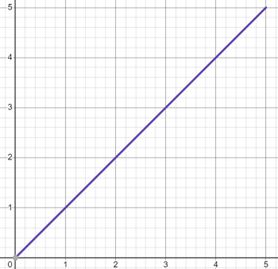
\includegraphics[width=0.7\textwidth]{pic/711.png}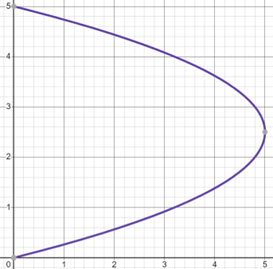
\includegraphics[width=0.7\textwidth]{pic/712.png}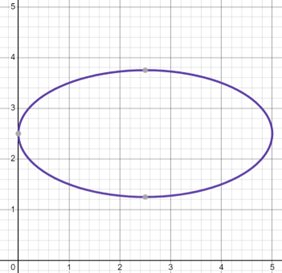
\includegraphics[width=0.7\textwidth]{pic/713.png} }
\end{minipage}
\end{figure}

---------------

Автор -- Тимур Гонтарь, М3206\question
Приведите  пример  нескольких бинарных отношений:
\begin{enumerate}
	\renewcommand{\labelenumi}{\alph{enumi})}
	\item отношение, которое является композиции нескольких бинарных отношений,  которое  нестрого порядка и функционально (укажите все бинарные отношения, участвующие в композиции)
	\item отношение, которое частично упорядочивает множество и как минимум 6 элементов упорядочены (обязательно покажите порядок элементов множества, полученный упордочиванием бинарным отношением)
	\item отношение, такое что обратное к нему  обладает одинаковыми с ним свойствами и оба эквивалентны (докажите, что свойства сохранаются)
\end{enumerate}

\underline{примечание:} важно показать  множества, на которых задано бинарное отношение и доказать, что ваше бинарное отношение обладает заданными свойствами
\question
Два контрабандиста затеяли сделку. Им кажется, что все должно пройти гладко и их план идеален, но стражи порядка уже взялись за это дело и планируют встать между ними, сорвав аферу. $\{1, 2, 3, 0\}$ – товары, которые планирует передать контрабандист $A$. $\{1, 2, 3, 4\}$ – планирует передать $B$. $A$, ничего не подозревая, уже готов передать две штуки товара 1 в руки полицейскому (притворившегося контрабандистом $B$) в обмен на 1 и 3 товар подставного $B$, две штуки товарa 2 – тоже в обмен на 1 и 3 товар. Также полиция связалась с $B$ по поводу передачи товара 3 в обмен на 4, и 3 на 1. Таким образом, если у полиции получилось перехватить сделки с обоих концов – работа выполена, и товар не окажется в руках ни у $A$ ни у $B$. Какие и сколько сделок полиции удалось предотвратить?
\\
---------------

Автор -- Мария Баженова, М3219\question
Даны отношения $R_1$, $R_2$ и $R_3$ на множестве $A = \{1; 2; 3; 4; 5;\}$ 
\begin{enumerate}
	\renewcommand{\labelenumi}{\alph{enumi})}
	\item $R_1 = \{(1; 1); (2; 2); (3; 3); (2; 1); (1; 2); \}$
	\item $R_2 = \{(1; 1); (2; 2); (1; 3); (3; 4); (3; 5);\}$
	\item $R_2 = \{(1; 1); (2; 2);  (1; 5); (3; 4); (3; 5); (4; 5)\}$
\end{enumerate}

\begin{enumerate}
	\renewcommand{\labelenumi}{\alph{enumi})}
	\item $R_1 \cap R_2$
	\item $R_1 \cup R_2 \cup R_3$
	\item $R_1^2 \cap R_3^{-1}$
	\item $R_1 \cup R_3^4$
	\item $R_1 \cup \overline{R_3}$
\end{enumerate}

определите основные свойства, получившихся отношений
определите какие свойства сохраняются относительно исходных отношений $R_1$, $R_2$ и $R_3$ 

\underline{примечание:} результатом может быть пустое множество

\end{questions}
\newpage
%%% begin test
\begin{flushright}
\begin{tabular}{p{2.8in} r l}
%\textbf{\class} & \textbf{ФИО:} & \makebox[2.5in]{\hrulefill}\\
\textbf{\class} & \textbf{ФИО:} &Галахова Виктория Кирилловна
\\

\textbf{\examdate} &&\\
%\textbf{Time Limit: \timelimit} & Teaching Assistant & \makebox[2in]{\hrulefill}
\end{tabular}\\
\end{flushright}
\rule[1ex]{\textwidth}{.1pt}


\begin{questions}
\question
Вы -- великая искательница сокровищ Лариса Крафтовое. Очередное путешествие забросило вас в подземные гробницы Сигизмунда I. К сожалению, на вашем пути встал очень назойливый мраморный привратник, который по всем канонам жанра имеет для вас пару загадок.
\\
\\
Привратник загадывает свое множество $X$, а также дает вам парочку других $(A,B,C…)$, объединяя, пересекая, дополняя и/или выполняя разность над которыми вы должны получить его множество. Загвоздка лишь в том, что привратник сам выбирает расстановку множеств в формуле, поэтому вам остается лишь вставить операции и расставить скобки (при надобности).

\paragraph{Загадка 1:}
\begin{equation*}
    X=\{2,3\}
\end{equation*}
\begin{equation*}
    A=\{1,2,3\}; B=\{3,4,5\}; C=\{1,4,5\}; D=\{2,3,5\}
    \end{equation*}
\begin{equation*}
    A ? B ? C ? D ? A ? C = X
\end{equation*}

\paragraph{Загадка 2:}
\begin{equation*}
    X=\{5,6\}
\end{equation*}
\begin{equation*}
    A=\{1,2,3,4\}; B=\{2,4,6\}; C=\{1,3,5\}
    \end{equation*}
\begin{equation*}
    A ? B ? C ? A = X
\end{equation*}

---------------

Автор -- Константин Васильев, М3213\question
Упростите следующее выражение с учетом того, что $A\subset B \subset C \subset D \subset U; A \neq \emptyset$
\begin{equation*}
	A \cap B  \cap \overline{C} \cup \overline{C} \cap D \cup B \cap C \cap D
\end{equation*}

Примечание: $U$ -- универсум\question
Укажите номера множеств, являющихся подмножествами множества
\begin{equation*}
	Q = \bar{A} \cap C \cup A \cap \bar{B} \cup A \cap \bar{C} \cup \bar{A} \cap B \cap D
\end{equation*}

\begin{enumerate}
	\renewcommand{\labelenumi}{\arabic{enumi})}
	\item $P = B \cap C \cap D \cup \bar{A} \cap B \cap C$;
	\item $P = \bar{B} \cap \bar{C} \cap D \cup B \cap \bar{C} \cap \bar{D}$;
	\item $P = A \cap \bar{B} \cap D \cup A \cap C \cap D$;
	\item $P = \bar{B} \cap \bar{C} \cup \bar{A} \cap \bar{B} \cap D$.
\end{enumerate}
\question
Постройте разбиения множеств:
\begin{enumerate}
	\renewcommand{\labelenumi}{\alph{enumi})}
	\item $A = \{6, 7, 8, 9, 11, 14, 34, 91, 55, 65, 76, 28, 19, 93, 94, \};$
	\item $B = \{0, 1, 2, 3, 4, 5, 6, 7, 8, 9, 11, 22, 33, 44, 55, 65, 111, 113, 67, 87, 91, 92, 93, 94, 95, 98\}$
	\item $A \cup B$
	\item $A \cap B$
\end{enumerate}
Таким образом, чтобы все разбиения имели как минимум 2 одинаковых множества в разбиениях.
Мощность каждого разбиение была более 4.
Докажите, что ваш ответ соответствует указанным условиям!\question
Пусть у нас есть $P$ -- множество студентов города Санкт-Петербург, из них $A$ -- третьекурсники, $B$ -- проходят профессиональную переподготовку, а $C$ -- стажируются в Яндексе. Для статьи “Как учиться на третьем курсе университета ИТМО, проходить профессиональную подготовку и не умереть” Мегабайт создал выборку $D$.
\\
\\
Упростите множество $E = (P \cap D \cup C \cap \overline{B} \cap \overline{D} \cup B \cap A \cap \overline{C}) \cap \overline{C} \cap \overline{D} \cap P$, а затем опишите его словами.
\\
\\
---------------

Автор -- Антонина Чернова, М33081\question
Дано отношение на множестве $\{1, 2, 3, 4, 5\}$ 
\begin{equation*}
	aRb \iff a \leqslant b
\end{equation*}

(ЧАСТЬ 1) Какими основным свойствами обладает отношение? (Дайте обоснованный ответ по всем пунктам ниже: докажите наличие или отсутствие свойств)  
\begin{enumerate}
	\renewcommand{\labelenumi}{\alph{enumi})}
	\item рефлексивность / антирефлексивность / нерефлексивность
	\item симметричность / антисимметричность / асимметричность / несимметричность
	\item транзитивность / антитранзитивность / нетранзитивность
\end{enumerate}

(ЧАСТЬ 2) Обоснуйте свой ответ по каждому из приведенных ниже вопросов:
\begin{enumerate}
	\renewcommand{\labelenumi}{\alph{enumi})}
    \item Является ли это отношение отношением эквивалентности?
    \item Является ли это отношение функциональным?
    \item Каким из отношений соответствия (одно-многозначным, много-многозначный и т.д.) оно является?
    \item К каким из отношений порядка (строгого, не строгого и т.д.) можно отнести данное отношение?
\end{enumerate}
\question
Установите, является ли каждое из перечисленных ниже отношений на А ($R \subseteq A \times A$) отношением эквивалентности (обоснование ответа обязательно). Для каждого отношения эквивалентности постройте классы 
эквивалентности и постройте граф отношения:
\begin{enumerate}
	\renewcommand{\labelenumi}{\alph{enumi})}
	\item А -- множество целых чисел и отношение $R = \{(a,b)|a + b = 5\}$
	\item Пусть A – множество имен. $A = \{ $Алексей, Иван, Петр, Александр, Павел, Андрей$ \}$. Тогда отношение $R $ верно на парах имен, начинающихся с одной и той же буквы, и только на них.
	\item На множестве $A = \{1; 2; 3; 4; 5\}$ задано отношение $R = \{(1; 2); (1; 3); (1; 5); (2; 3); (2; 4); (2; 5); (3; 4); (3; 5); (4; 5)\}$
\end{enumerate}\question
Приведите  пример  нескольких бинарных отношений:
\begin{enumerate}
	\renewcommand{\labelenumi}{\alph{enumi})}
	\item отношение, которое является композиции нескольких бинарных отношений,  которое  обладает любым типом соответсвия  и симметрично (укажите все бинарные отношения, участвующие в композиции)
	\item два отношения, первое -- частично упорядочивает множество, на котором оно задано и второе -- полностью упорядочивает (обязательно покажите порядок элементов множества, полученный упордочиванием бинарным отношением)
	\item отношение, такое что обратное к нему  обладает одинаковыми с ним свойствами и оба функциональны (докажите, что свойства сохранаются)
\end{enumerate}

\underline{примечание:} важно показать  множества, на которых задано бинарное отношение и доказать, что ваше бинарное отношение обладает заданными свойствами
\question
В перерыве между парами дискретной математики вы с друзьями решили зарубиться в домино. Иллюстрация ниже визуализирует данный момент игры.

\\
\begin{figure}[h]

\begin{minipage}[h]{0.55\linewidth}
\end{minipage}
\begin{minipage}[h]{0.45\linewidth}
\center{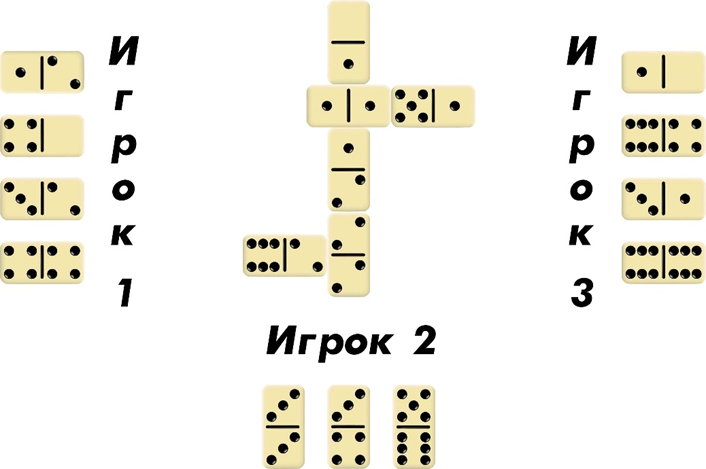
\includegraphics[width=0.7\textwidth]{pic/941.png} }
\end{minipage}
\end{figure}

Так как вы — умные студенты, вам стало интересно интерпретировать партию в виде бинарных отношений. Запишите отношения:
\begin{itemize}
    \item $G = \{(a,b)|a$ и $b$ – стороны свободных доминошек, лежащих на столе, где a – свободная сторона$\}$
    \item $R_1 = \{(a,b)|a$ и $b$ – стороны одной доминошки в руке у первого игрока$\}$
    \item $R_2 = \{(a,b)|a$ и $b$ – стороны одной доминошки в руке у второго игрока$\}$
    \item $R_3 = \{(a,b)|a$ и $b$ – стороны одной доминошки в руке у третьего игрока$\}$
\end{itemize}

Используя операцию композиции, составьте новые бинарные отношения:
\begin{itemize}
    \item $P_1$ – возможные ходы у первого игрока
    \item $P_2$ – возможные ходы у второго игрока
    \item $P_3$ – возможные ходы у третьего игрока
\end{itemize}


Ходом является пара крайних номеров стоящих рядом доминошек.
\\
---------------

Автор -- Константин Васильев, М3213\question
Даны отношения $R_1$, $R_2$ и $R_3$ на множестве $A = \{1; 2; 3; 4; 5;\}$ 
\begin{enumerate}
	\renewcommand{\labelenumi}{\alph{enumi})}
	\item $R_1 = \{(3; 2); (3; 1); (1; 3)\}$
	\item $R_2 = \{(1; 2); (2; 2); (1; 3); (4; 5)\}$
	\item $R_3 = \{(1; 2); (2; 2); (3; 4); (3; 5); (4; 5)\}$
\end{enumerate}

\begin{enumerate}
	\renewcommand{\labelenumi}{\alph{enumi})}
	\item $R_1 \cap R_2^{-1} \cup R_3^2$
	\item $(R_1 \cup R_2) \cap R_3$
	\item $R_3^2 \cap R_3^{-1}$
	\item $R_3^{-1} \cup \overline{R_2^{-1}}$
	\item $R_1^{-1} \cup \overline{R_2} \cup R_3$
\end{enumerate}

определите основные свойства, получившихся отношений
определите какие свойства сохраняются относительно исходных отношений $R_1$, $R_2$ и $R_3$ 

\underline{примечание:} результатом может быть пустое множество

\end{questions}
\newpage
%%% begin test
\begin{flushright}
\begin{tabular}{p{2.8in} r l}
%\textbf{\class} & \textbf{ФИО:} & \makebox[2.5in]{\hrulefill}\\
\textbf{\class} & \textbf{ФИО:} &Гималетдинова Светлана Дамировна
\\

\textbf{\examdate} &&\\
%\textbf{Time Limit: \timelimit} & Teaching Assistant & \makebox[2in]{\hrulefill}
\end{tabular}\\
\end{flushright}
\rule[1ex]{\textwidth}{.1pt}


\begin{questions}
\question
Вы -- великая искательница сокровищ Лариса Крафтовое. Очередное путешествие забросило вас в подземные гробницы Сигизмунда I. К сожалению, на вашем пути встал очень назойливый мраморный привратник, который по всем канонам жанра имеет для вас пару загадок.
\\
\\
Привратник загадывает свое множество $X$, а также дает вам парочку других $(A,B,C…)$, объединяя, пересекая, дополняя и/или выполняя разность над которыми вы должны получить его множество. Загвоздка лишь в том, что привратник сам выбирает расстановку множеств в формуле, поэтому вам остается лишь вставить операции и расставить скобки (при надобности).

\paragraph{Загадка 1:}
\begin{equation*}
    X=\{1,2,5,6\}
\end{equation*}
\begin{equation*}
    A=\{1,2,3,4\}; B=\{2,3,4,5\}; C=\{2,5\}; D=\{4,5,6\}
    \end{equation*}
\begin{equation*}
    A ? B ? C ? D = X
\end{equation*}

\paragraph{Загадка 2:}
\begin{equation*}
    X=\{3,4,5\}
\end{equation*}
\begin{equation*}
    A=\{2,3,4,5\}; B=\{1,2,3\}; C=\{3,4,5\}; D=\{1,5,6\}
    \end{equation*}
\begin{equation*}
    A ? B ? C ? D = X
\end{equation*}

---------------

Автор -- Константин Васильев, М3213\question
Упростите следующее выражение с учетом того, что $A\subset B \subset C \subset D \subset U; A \neq \emptyset$
\begin{equation*}
	A \cap  \overline{C} \cup B \cap \overline{D} \cup  \overline{A} \cap C \cap  \overline{D}
\end{equation*}

Примечание: $U$ -- универсум\question
Укажите номера множеств, являющихся подмножествами множества
\begin{equation*}
	Q = A \cap \bar{D} \cup B \cap C \cup \bar{A} \cap \bar{B} \cap D \cup A \cap C
\end{equation*}

\begin{enumerate}
	\renewcommand{\labelenumi}{\arabic{enumi})}
	\item $P = A \cap \bar{B} \cap D \cup \bar{A} \cap \bar{B} \cap C$;
	\item $P = A \cap B \cap D \cup \bar{A} \cap \bar{C} \cap D$;
	\item $P = B \cap \bar{C} \cap \bar{D} \cup A \cap B \cap \bar{C}$;
	\item $P = A \cap \bar{C} \cap \bar{D} \cup \bar{A} \cap \bar{B} \cap D$.
\end{enumerate}
\question
Постройте разбиения множеств:
\begin{enumerate}
	\renewcommand{\labelenumi}{\alph{enumi})}
	\item $A = \{6, 7, 8, 9, 11, 14, 34, 54, 91\};$
	\item $B = \{0, 1, 2, 3, 4, 5, 6, 7, 8, 9\}$
	\item $A \cap B$
\end{enumerate}
Таким образом, чтобы все разбиения имели как минимум 2 одинаковых множества в разбиениях.
Мощность каждого разбиение была более 6.
Докажите, что ваш ответ соответствует указанным условиям!\question
Упростить выражения, используя свойства операций над множествами:

\begin{enumerate}
	\renewcommand{\labelenumi}{\alph{enumi})}
	\item $(\bar{A} \cup B \cup \bar{C}) \cap(A \cap \bar{B} \cap C) \cap \overline{(A \cup C)}$;
	\item $(A\cap B \cap C \cap D) \cup (\overline{\overline{A}\cup C}\cap D) \cup (D\cap\overline{(\overline{A}+C)+D})\cup (\overline{A}\cap B\cap C \cap D)$.
\end{enumerate}
\question
Довольные студенты ИТМО сдали летнюю сессию и намерены поехать домой на некоторое время. К сожалению, чтобы добраться до пункта назначения, им потребуется сделать несколько пересадок.

Пусть множество всех населенных пунктов выглядит как: $A = \{1, 2, 3, 4, 5, 6\}$.
\\
Тогда $R = \{(1, 3), (3, 1), (2, 4), (4, 2), (1, 5), (5, 1), (2, 3), (3, 2)\}$ -- можно доехать на автобусе, $S = \{(5, 6), (6, 5), (3, 6), (6, 3)\}$ -- можно долететь на самолете.
\\
Какими свойствами обладают отношения R и S?
\\
---------------

Автор -- Елизавета Котельникова, М3212\question
Установите, является ли каждое из перечисленных ниже отношений на А ($R \subseteq A \times A$) отношением эквивалентности (обоснование ответа обязательно). Для каждого отношения эквивалентности постройте классы 
эквивалентности и постройте граф отношения:
\begin{enumerate}
	\renewcommand{\labelenumi}{\alph{enumi})}
	\item $A = \{a, b, c, d, p, t\}$ задано отношение $R = \{(a, a), (b, b), (b, c), (b, d), (c, b), (c, c), (c, d), (d, b), (d, c), (d, d), (p,p), (t,t)\}$
	\item $A = \{-10, -9, ..., 9, 10\}$ и отношение $R = \{(a,b)|a^{3} = b^{3}\}$
	\item $F(x)=x^{2}+1$, где $x \in A = [-2, 4]$ и отношение $R = \{(a,b)|F(a) = F(b)\}$
\end{enumerate}\question
Приведите  пример  нескольких бинарных отношений:
\begin{enumerate}
	\renewcommand{\labelenumi}{\alph{enumi})}
	\item отношение, которое является композиции нескольких бинарных отношений,  которое  обладает любым типом соответсвия  и симметрично (укажите все бинарные отношения, участвующие в композиции)
	\item два отношения, первое -- частично упорядочивает множество, на котором оно задано и второе -- полностью упорядочивает (обязательно покажите порядок элементов множества, полученный упордочиванием бинарным отношением)
	\item отношение, такое что обратное к нему  обладает одинаковыми с ним свойствами и оба функциональны (докажите, что свойства сохранаются)
\end{enumerate}

\underline{примечание:} важно показать  множества, на которых задано бинарное отношение и доказать, что ваше бинарное отношение обладает заданными свойствами
\question
Довольные студенты ИТМО сдали летнюю сессию и намерены поехать домой на некоторое время. К сожалению, чтобы добраться до пункта назначения, им потребуется сделать несколько пересадок.

Пусть множество всех населенных пунктов выглядит как: $A = \{1, 2, 3, 4, 5, 6\}$.
\\
Тогда $R = \{(1, 3), (3, 1), (2, 4), (4, 2), (1, 5), (5, 1), (2, 3), (3, 2)\}$ -- можно доехать на автобусе, $S = \{(5, 6), (6, 5), (3, 6), (6, 3)\}$ -- можно долететь на самолете.

\begin{itemize}
    \item Найдите такие пары пунктов, для перемещения между которыми надо проехать на автобусе, а затем воспользоваться самолетом и наоборот.
    \item Найдите пары пунктов, между которыми можно перемещаться на автобусе с одной пересадкой (пары вида (1, 1) не стоит указывать в ответе).
    \item Найдите пары пунктов, между которыми можно перемещаться на самолете с одной пересадкой в промежуточном пункте.
\end{itemize}
\\
---------------

Автор -- Елизавета Котельникова, М3212\question
Даны отношения $R_1$, $R_2$ и $R_3$ на множестве $A = \{1; 2; 3; 4; 5;\}$ 
\begin{enumerate}
	\renewcommand{\labelenumi}{\alph{enumi})}
	\item $R_1 = \{(1; 1); (2; 2); (3; 3); (2; 1);  (3; 1); (1; 3)\}$
	\item $R_2 = \{(1; 2); (2; 2); (3; 4); (3; 5); (4; 5)\}$
	\item $R_2 = \{(1; 3); (1; 5); (3; 4); (3; 5); (4; 5)\}$
\end{enumerate}

\begin{enumerate}
	\renewcommand{\labelenumi}{\alph{enumi})}
	\item $(R_1 \cap R_2) \cup R_3$
	\item $R_1 \cup R_3$
	\item $R_1^3 \cap R_3^-1$
	\item $R_3 \cup R_2^2$
	\item $R_2 \cup \overline{R_1}$
\end{enumerate}

определите основные свойства, получившихся отношений
определите какие свойства сохраняются относительно исходных отношений $R_1$, $R_2$ и $R_3$ 

\underline{примечание:} результатом может быть пустое множество

\end{questions}
\newpage
%%% begin test
\begin{flushright}
\begin{tabular}{p{2.8in} r l}
%\textbf{\class} & \textbf{ФИО:} & \makebox[2.5in]{\hrulefill}\\
\textbf{\class} & \textbf{ФИО:} &Дюбченко Ангелина Андреевна
\\

\textbf{\examdate} &&\\
%\textbf{Time Limit: \timelimit} & Teaching Assistant & \makebox[2in]{\hrulefill}
\end{tabular}\\
\end{flushright}
\rule[1ex]{\textwidth}{.1pt}


\begin{questions}
\question
Ребята приехали в математический лагерь, где каждый получил футболку с уникальным номером от 1 до 23. Отправившись на очередной полдник, они обнаружили, что нет ни одного кекса – их украли! Ребята сразу приступили к расследованию. Таким образом, они сделали вывод, что виновник – не один человек, а целая группа! У них получилось разделить всех ребят на 4 группы подозреваемых, в зависимости от того, кто где был в предположительное время совершения преступления по словам очевидцев.
\\(Легенда: С – столовая, D – двор, B – баскетбольная площадка, А - аллея): 
\begin{center}
$A: \{1, 2, 3, 21, 23, 5, 22, 18, 19, 6\}$
\\
$B: \{6, 22, 10, 15, 11, 13, 7, 18, 14, 9\}$
\\
$C: \{7, 8, 14, 20, 12, 4, 1, 2, 19, 6\}$
\\
$D: \{9, 13, 16, 17, 18, 19, 22, 14, 5, 6\}$
\end{center}
Так как ребята были отличными математиками, у них получилось составить выражение, которое раскроет, кто виноват в преступлении. 
\begin{equation*}
    A \cup B \cap \overline{C} \cup (A \cap D \cup \overline{C}) \cup D
\end{equation*}
Помогите им найти виновных.

---------------

Автор -- Баженова Мария, М3219\question
Упростите следующее выражение с учетом того, что $A\subset B \subset C \subset D \subset U; A \neq \emptyset$
\begin{equation*}
	A \cap C  \cap D \cup B \cap \overline{C} \cap D \cup B \cap C \cap D
\end{equation*}

Примечание: $U$ -- универсум\question
Укажите номера множеств, являющихся подмножествами множества
\begin{equation*}
	Q = \bar{A} \cap C \cup A \cap \bar{B} \cup A \cap \bar{C} \cup \bar{A} \cap B \cap D
\end{equation*}

\begin{enumerate}
	\renewcommand{\labelenumi}{\arabic{enumi})}
	\item $P = A \cap \bar{B} \cap D \cup \bar{A} \cap \bar{B} \cap C$;
	\item $P = A \cap B \cap D \cup \bar{A} \cap \bar{C} \cap D$;
	\item $P = B \cap \bar{C} \cap \bar{D} \cup A \cap B \cap \bar{C}$;
	\item $P = A \cap \bar{C} \cap \bar{D} \cup \bar{A} \cap \bar{B} \cap D$.
\end{enumerate}
\question
Постройте разбиения множеств:
\begin{enumerate}
	\renewcommand{\labelenumi}{\alph{enumi})}
	\item $A = \{6, 7, 8, 9, 11, 14, 34, 91, 55, 65, 76, 28, 19\};$
	\item $B = \{0, 1, 2, 3, 4, 8, 9, 11, 22, 33, 44, 55, 65, 76, 28, 19\}$
	\item $A \cup B$
	\item $A \cap B$
\end{enumerate}
Таким образом, чтобы все разбиения имели как минимум 2 одинаковых множества в разбиениях.
Мощность каждого разбиение была более 4.
Докажите, что ваш ответ соответствует указанным условиям!\question
Упростить выражения, используя свойства операций над множествами:

\begin{enumerate}
	\renewcommand{\labelenumi}{\alph{enumi})}
	\item $(A\cap B \cap C \cap D) \cup (\overline{\overline{A}\cup C}\cap D) \cup (D\cap\overline{(\overline{A}+C)+D})\cup (\overline{A}\cap B\cap C \cap D)$;
	\item $(A\cap B \cap C \cap D \cap (A\cup D \cup \overline{A\cap D}))\cup \overline{\overline{A}\cup \overline{D}\cup C\cup D}\cup (A\cap B \cap (D\cap\overline{C}\cup C\cap\overline{D}))$.
\end{enumerate}
\question
Бабушка Люда потеряла книгу со своими лучшими рецептами напитков. Вы, как добросовестный внук, проводивший у любимой бабушки большое количество времени, помните из чего бабуля варила вкуснейшие морсы и компоты. Обычно бабушка варила напитки из двух видов ягод и фруктов среди которых были: Малина, Облепиха, Жимолость, Смородина, Яблоки, Абрикосы и Груши. Также вы помните, что нельзя совмещать между собой Облепиху и красные ягоды, Абрикос и ягоды, Яблоко и ягоды. Постройте бинарное отношение содержащее все возможные сочетания для напитков таким образом, чтобы ингредиенты не повторялись.
\\
Ответьте на вопросы касаемо построенного бинарного отношения:
\begin{itemize}
    \item Какими свойствами обладает данное БО? Обоснуйте
    \item Является ли данное отношение функциональным?
    \item Каким из отношений соответствия оно является? (одно-многозначным, много-многозначным и т.д.)
\end{itemize}
\\
---------------

Автор -- Максим Акимцов, М3208\question
Дана декартова система координат. Ось $x$ представляет собой множество $X$, ось $y$ - множество $Y$. На этих двух множествах определены бинарные отношения, которые схематически изображены в виде графиков выше (то есть, например, для графика с рис. 1 будет верно, что пары $(0, 0), (1, 1), (2, 2), (3, 3), (4, 4), (5, 5)$ входят в бинарное отношение, соответствующее графику). Для каждого из таких отношений определить:
\begin{itemize}
    \item Каким типом отношения соответствия оно является?
    \item Является ли оно функциональным отношением? Если да, то каким именно (сюръекция, инъекция, биекция)?
\end{itemize}
Обоснуйте своё решение. После этого, аналогично данным в условии графикам, придумайте отношение (любое), которое будет представлять собой полностью определенную функцию, и при этом будет инъективно и не сюръективно.
\\
\begin{figure}[h]

\begin{minipage}[h]{0.55\linewidth}
\end{minipage}
\begin{minipage}[h]{0.45\linewidth}
\center{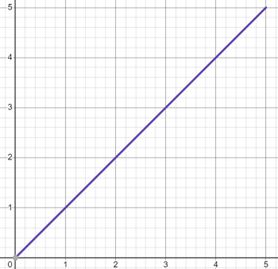
\includegraphics[width=0.7\textwidth]{pic/711.png}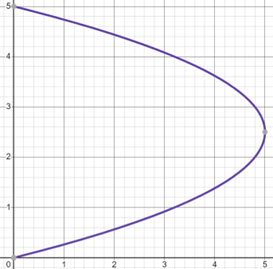
\includegraphics[width=0.7\textwidth]{pic/712.png}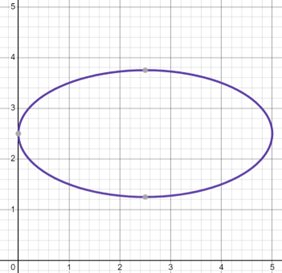
\includegraphics[width=0.7\textwidth]{pic/713.png} }
\end{minipage}
\end{figure}

---------------

Автор -- Тимур Гонтарь, М3206\question
Приведите  пример  нескольких бинарных отношений:
\begin{enumerate}
	\renewcommand{\labelenumi}{\alph{enumi})}
	\item отношение, которое является композиции нескольких бинарных отношений,  которое  обладает любым типом соответсвия  и симметрично (укажите все бинарные отношения, участвующие в композиции)
	\item два отношения, первое -- частично упорядочивает множество, на котором оно задано и второе -- полностью упорядочивает (обязательно покажите порядок элементов множества, полученный упордочиванием бинарным отношением)
	\item отношение, такое что обратное к нему  обладает одинаковыми с ним свойствами и оба функциональны (докажите, что свойства сохранаются)
\end{enumerate}

\underline{примечание:} важно показать  множества, на которых задано бинарное отношение и доказать, что ваше бинарное отношение обладает заданными свойствами
\question
Вася хочет устроиться бэкенд разработчиком в ИТМО, работать с ИСУ. На собеседовании тимлид дал ему тестовое задание, чтобы определить его уровень знаний:
\\
\begin{figure}[h]

\begin{minipage}[h]{0.55\linewidth}
\end{minipage}
\begin{minipage}[h]{0.45\linewidth}
\center{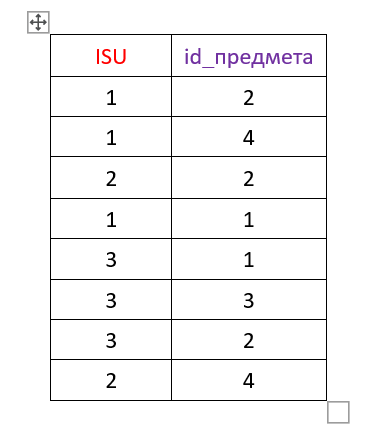
\includegraphics[width=0.7\textwidth]{pic/911.png}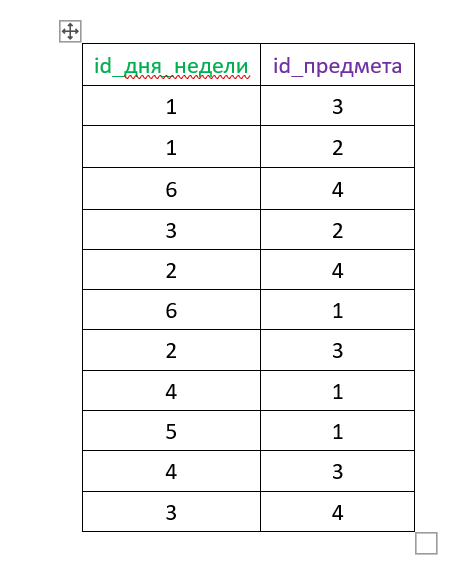
\includegraphics[width=0.7\textwidth]{pic/912.png} }
\end{minipage}
\end{figure}

В базе данных расписания ИТМО есть 2 таблицы:
\begin{itemize}
    \item В таблице 1 (рис. 1) каждому студенту по его номеру ИСУ сопоставлены предметы по их id. У одного номера ИСУ (студента) может быть много предметов, при этом на один предмет может ходить несколько студентов.
    \item В таблице 2 (рис. 2) каждому дню недели по его id (порядковый номер: 1-пн, 2-вт, 3-ср и т. д.) сопоставлены предметы по их id. В один день могут проводиться пары по нескольким предметам, при этом пары по одному предмету могут проходить несколько дней в неделе.
\end{itemize}
От Васи требуется по имеющимся данным вывести все возможные кортежи вида:

\begin{center}(номер ИСУ, день когда у этого студента есть пары)\end{center}

Например, ответ вида $\{(1, 1), (1, 5), (2, 1)\}$ будет означать что студент с ISU №1 имеет пары в понедельник и пятницу, а студент с ISU №2 имеет пары только в понедельник.

Помогите Васе решить данную задачу, используя ваши знания по дискретной математике.

---------------

Автор -- Тимур Гонтарь, М3206\question
Даны отношения $R_1$, $R_2$ и $R_3$ на множестве $A = \{1; 2; 3; 4; 5;\}$ 
\begin{enumerate}
	\renewcommand{\labelenumi}{\alph{enumi})}
	\item $R_1 = \{(1; 1); (2; 2); (3; 3); (2; 1);  (3; 1); (1; 3)\}$
	\item $R_2 = \{(1; 2); (2; 2); (3; 4); (3; 5); (4; 5)\}$
	\item $R_2 = \{(1; 3); (1; 5); (3; 4); (3; 5); (4; 5)\}$
\end{enumerate}

\begin{enumerate}
	\renewcommand{\labelenumi}{\alph{enumi})}
	\item $(R_1 \cap R_2) \cup R_3$
	\item $R_1 \cup R_3$
	\item $R_1^3 \cap R_3^-1$
	\item $R_3 \cup R_2^2$
	\item $R_2 \cup \overline{R_1}$
\end{enumerate}

определите основные свойства, получившихся отношений
определите какие свойства сохраняются относительно исходных отношений $R_1$, $R_2$ и $R_3$ 

\underline{примечание:} результатом может быть пустое множество

\end{questions}
\newpage
%%% begin test
\begin{flushright}
\begin{tabular}{p{2.8in} r l}
%\textbf{\class} & \textbf{ФИО:} & \makebox[2.5in]{\hrulefill}\\
\textbf{\class} & \textbf{ФИО:} &Иванов Пётр Александрович
\\

\textbf{\examdate} &&\\
%\textbf{Time Limit: \timelimit} & Teaching Assistant & \makebox[2in]{\hrulefill}
\end{tabular}\\
\end{flushright}
\rule[1ex]{\textwidth}{.1pt}


\begin{questions}
\question
Вы -- великая искательница сокровищ Лариса Крафтовое. Очередное путешествие забросило вас в подземные гробницы Сигизмунда I. К сожалению, на вашем пути встал очень назойливый мраморный привратник, который по всем канонам жанра имеет для вас пару загадок.
\\
\\
Привратник загадывает свое множество $X$, а также дает вам парочку других $(A,B,C…)$, объединяя, пересекая, дополняя и/или выполняя разность над которыми вы должны получить его множество. Загвоздка лишь в том, что привратник сам выбирает расстановку множеств в формуле, поэтому вам остается лишь вставить операции и расставить скобки (при надобности).

\paragraph{Загадка 1:}
\begin{equation*}
    X=\{2,3\}
\end{equation*}
\begin{equation*}
    A=\{1,2,3\}; B=\{3,4,5\}; C=\{1,4,5\}; D=\{2,3,5\}
    \end{equation*}
\begin{equation*}
    A ? B ? C ? D ? A ? C = X
\end{equation*}

\paragraph{Загадка 2:}
\begin{equation*}
    X=\{5,6\}
\end{equation*}
\begin{equation*}
    A=\{1,2,3,4\}; B=\{2,4,6\}; C=\{1,3,5\}
    \end{equation*}
\begin{equation*}
    A ? B ? C ? A = X
\end{equation*}

---------------

Автор -- Константин Васильев, М3213\question
Упростите следующее выражение с учетом того, что $A\subset B \subset C \subset D \subset U; A \neq \emptyset$
\begin{equation*}
	\overline{A} \cap \overline{B} \cup B \cap \overline{C} \cup \overline{C} \cap D
\end{equation*}

Примечание: $U$ -- универсум\question
Укажите номера множеств, являющихся подмножествами множества
\begin{equation*}
	Q = A \cap \bar{D} \cup B \cap C \cup \bar{A} \cap \bar{B} \cap D \cup A \cap C
\end{equation*}

\begin{enumerate}
	\renewcommand{\labelenumi}{\arabic{enumi})}
	\item $P = A \cap \bar{B} \cap D \cup \bar{A} \cap \bar{B} \cap C$;
	\item $P = A \cap B \cap D \cup \bar{A} \cap \bar{C} \cap D$;
	\item $P = B \cap \bar{C} \cap \bar{D} \cup A \cap B \cap \bar{C}$;
	\item $P = A \cap \bar{C} \cap \bar{D} \cup \bar{A} \cap \bar{B} \cap D$.
\end{enumerate}
\question
Постройте разбиения множеств:
\begin{enumerate}
	\renewcommand{\labelenumi}{\alph{enumi})}
	\item $A = \{6, 7, 8, 9, 11, 14, 34, 54, 47, 18, 91, 55, 65, 76, 28, 19\};$
	\item $B = \{0, 11, 22, 33, 44, 55, 65, 76, 28, 19\}$
	\item $A \cup B$
\end{enumerate}
Таким образом, чтобы все разбиения имели как минимум 2 одинаковых множества в разбиениях.
Мощность каждого разбиение была более 3.
Докажите, что ваш ответ соответствует указанным условиям!
\question
Упростить выражения, используя свойства операций над множествами:

\begin{enumerate}
	\renewcommand{\labelenumi}{\alph{enumi})}
	\item $(\bar{A} \cup B \cup \bar{C}) \cap(A \cap \bar{B} \cap C) \cap \overline{(A \cup C)}$;
	\item $(A\cap B \cap C \cap D) \cup (\overline{\overline{A}\cup C}\cap D) \cup (D\cap\overline{(\overline{A}+C)+D})\cup (\overline{A}\cap B\cap C \cap D)$.
\end{enumerate}
\question
Определить и обосновать, являются ли рефлексивными/симметричными/транзитивными, отношениями порядка, одно-однозначными/одно-многозначными/много-однозначными/много-многозначными бинарные отношения:
\begin{itemize}
    \item $aRb \Leftrightarrow a$ является ребёнком $b$ ($a$ и $b$ -- люди)
    \item $aRb \Leftrightarrow a$ и $b$ живут в одной стране ($a$ и $b$ -- люди)
    \item $aRb \Leftrightarrow a$ охотится на $b$ ($a$ и $b$ -- животные)
\end{itemize}
\\
Выделите среди этих БО отношения эквивалентности и разбейте их на классы эквивалентности, продемонстрировав алгоритм разбиения.
\\
---------------

Автор -- Алексей Лёвушкин, М3204\question
Дана декартова система координат. Ось $x$ представляет собой множество $X$, ось $y$ - множество $Y$. На этих двух множествах определены бинарные отношения, которые схематически изображены в виде графиков выше (то есть, например, для графика с рис. 1 будет верно, что пары $(0, 0), (1, 1), (2, 2), (3, 3), (4, 4), (5, 5)$ входят в бинарное отношение, соответствующее графику). Для каждого из таких отношений определить:
\begin{itemize}
    \item Каким типом отношения соответствия оно является?
    \item Является ли оно функциональным отношением? Если да, то каким именно (сюръекция, инъекция, биекция)?
\end{itemize}
Обоснуйте своё решение. После этого, аналогично данным в условии графикам, придумайте отношение (любое), которое будет представлять собой полностью определенную функцию, и при этом будет инъективно и не сюръективно.
\\
\begin{figure}[h]

\begin{minipage}[h]{0.55\linewidth}
\end{minipage}
\begin{minipage}[h]{0.45\linewidth}
\center{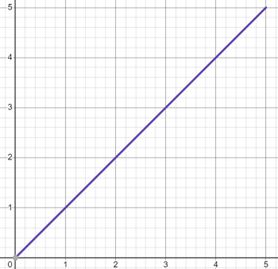
\includegraphics[width=0.7\textwidth]{pic/711.png}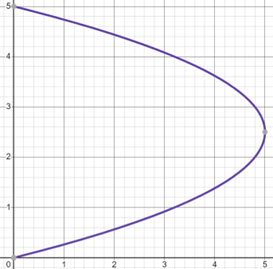
\includegraphics[width=0.7\textwidth]{pic/712.png}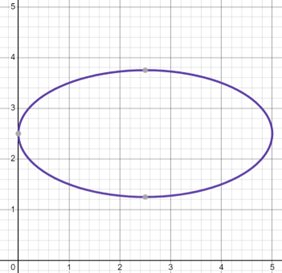
\includegraphics[width=0.7\textwidth]{pic/713.png} }
\end{minipage}
\end{figure}

---------------

Автор -- Тимур Гонтарь, М3206\question
Приведите  пример  нескольких бинарных отношений:
\begin{enumerate}
	\renewcommand{\labelenumi}{\alph{enumi})}
	\item отношение, которое является композиции нескольких бинарных отношений,  которое  нестрого порядка и функционально (укажите все бинарные отношения, участвующие в композиции)
	\item отношение, которое частично упорядочивает множество и как минимум 6 элементов упорядочены (обязательно покажите порядок элементов множества, полученный упордочиванием бинарным отношением)
	\item отношение, такое что обратное к нему  обладает одинаковыми с ним свойствами и оба эквивалентны (докажите, что свойства сохранаются)
\end{enumerate}

\underline{примечание:} важно показать  множества, на которых задано бинарное отношение и доказать, что ваше бинарное отношение обладает заданными свойствами
\question
Петя решил поучаствовать в конкурсе рисунков, к сожалению, проблема была в том, что он совершенно не умел рисовать, но Петя был умным мальчиком, который знал бинарные отношения.
\\На декартовом произведении множества $A = \{-2, -1, 0, 1, 2, 3, 4, 5, 6, 7, 8, 9, 10, 11\}$ заданы бинарные отношения:
\begin{equation*}
R_1 = {(0, -2), (2, 0), (6, -2), (8, 0), (9, -2), (12, -2), (11, -1), (11, 1), (12, 2), (9, 2), (8, 0), (6, 2), (5, 5), (0, 5), (6, 7), (0, 6)}
\end{equation*}
\begin{center}и\end{center}
\begin{equation*}
R_2 = \{(10, -1), (10, -1), (9, 0)\}
\end{equation*}
Помогите Пете выиграть в конкурсе! Постройте композиции отношений $R_1^{-1}, R_2^{-1}$ и изобразите полученный результат на декартовой системе координат (задание можно дополнять другими композициями).
\\
---------------

Автор -- Анастасия Стеценко, М3207\question
Даны отношения $R_1$, $R_2$ и $R_3$ на множестве $A = \{1; 2; 3; 4; 5;\}$ 
\begin{enumerate}
	\renewcommand{\labelenumi}{\alph{enumi})}
	\item $R_1 = \{(3; 2); (3; 1); (1; 3)\}$
	\item $R_2 = \{(1; 2); (2; 2); (1; 3); (1; 5); (2; 3); (4; 5)\}$
	\item $R_2 = \{(1; 2); (2; 2); (3; 4); (3; 5); (4; 5)\}$
\end{enumerate}

\begin{enumerate}
	\renewcommand{\labelenumi}{\alph{enumi})}
	\item $R_1 \cap R_2$
	\item $(R_1 \cup R_2) \cap R_3$
	\item $R_3^2 \cap R_3^{-1}$
	\item $R_3 \cup \overline{R_2^2}$
	\item $R_1 \cup \overline{R_2} \cup R_3$
\end{enumerate}

определите основные свойства, получившихся отношений
определите какие свойства сохраняются относительно исходных отношений $R_1$, $R_2$ и $R_3$ 

\underline{примечание:} результатом может быть пустое множество

\end{questions}
\newpage
%%% begin test
\begin{flushright}
\begin{tabular}{p{2.8in} r l}
%\textbf{\class} & \textbf{ФИО:} & \makebox[2.5in]{\hrulefill}\\
\textbf{\class} & \textbf{ФИО:} &Каримов Максим Дмитриевич
\\

\textbf{\examdate} &&\\
%\textbf{Time Limit: \timelimit} & Teaching Assistant & \makebox[2in]{\hrulefill}
\end{tabular}\\
\end{flushright}
\rule[1ex]{\textwidth}{.1pt}


\begin{questions}
\question
Пусть у нас есть $P$ -- множество студентов города Санкт-Петербург, из них $A$ -- третьекурсники, $B$ -- проходят профессиональную переподготовку, а $C$ -- стажируются в Яндексе. Для статьи “Как учиться на третьем курсе университета ИТМО, проходить профессиональную подготовку и не умереть” Мегабайт создал выборку $D$.

Студенты ИТМО участвуют в специальной лотерее. Мы спросили номера лотерейных билетов некоторых из них. Получилась такая статистика:

\begin{center}
$A = \{1, 3, 7, 12, 15, 19, 22\}$
\\
$B = \{2, 3, 7, 9, 13, 16, 18, 21, 24\}$
\\
$C = \{2, 4, 5, 8, 10, 11, 13, 14, 17, 21, 23\}$
\\
$D = \{1, 2, 9, 13, 16, 19, 21, 22, 24\}$
\end{center}

Помогите Мегабайту понять, какие номера билетов у студентов из их выборки, которые стажируются в Яндексе.

---------------

Автор -- Антонина Чернова, М33081\question
Упростите следующее выражение с учетом того, что $A\subset B \subset C \subset D \subset U; A \neq \emptyset$
\begin{equation*}
	A \cap C  \cap D \cup B \cap \overline{C} \cap D \cup B \cap C \cap D
\end{equation*}

Примечание: $U$ -- универсум\question
Укажите номера множеств, являющихся подмножествами множества
\begin{equation*}
	Q = \bar{A} \cap C \cup A \cap \bar{B} \cup A \cap \bar{C} \cup \bar{A} \cap B \cap D
\end{equation*}

\begin{enumerate}
	\renewcommand{\labelenumi}{\arabic{enumi})}
	\item $P = B \cap C \cap D \cup \bar{A} \cap B \cap C$;
	\item $P = \bar{B} \cap \bar{C} \cap D \cup B \cap \bar{C} \cap \bar{D}$;
	\item $P = A \cap \bar{B} \cap D \cup A \cap C \cap D$;
	\item $P = \bar{B} \cap \bar{C} \cup \bar{A} \cap \bar{B} \cap D$.
\end{enumerate}
\question
Постройте разбиения множеств:
\begin{enumerate}
	\renewcommand{\labelenumi}{\alph{enumi})}
	\item $A = \{6, 7, 8, 9, 11, 14, 34, 54, 47, 18, 91\};$
	\item $B = \{0, 1, 2, 3, 4, 5, 6, 7, 8, 9\}$
	\item $A \cap B$
\end{enumerate}
Таким образом, чтобы все разбиения имели как минимум 2 одинаковых множества в разбиениях.
Мощность каждого разбиение была более 3.
Докажите, что ваш ответ соответствует указанным условиям!\question
Упростить выражения, используя свойства операций над множествами:

\begin{enumerate}
	\renewcommand{\labelenumi}{\alph{enumi})}
	\item $(A\cap B \cap C \cap D) \cup (\overline{\overline{A}\cup C}\cap D) \cup (D\cap\overline{(\overline{A}+C)+D})\cup (\overline{A}\cap B\cap C \cap D)$;
	\item $(A\cap B \cap C \cap D \cap (A\cup D \cup \overline{A\cap D}))\cup \overline{\overline{A}\cup \overline{D}\cup C\cup D}\cup (A\cap B \cap (D\cap\overline{C}\cup C\cap\overline{D}))$.
\end{enumerate}
\question
Возьмём множество $M = \{1, 2, 3, 4, 5, 6, 7, 8, 9\}$. Определите свойства и виды бинарных отношений:
\begin{itemize}
    \item $xRy \Leftrightarrow x$ делит $y$
    \item $xRy \Leftrightarrow x + y = 8$
    \item $xRy \Leftrightarrow x + y \in M$
\end{itemize}
---------------

Автор -- Алексей Лёвушкин, М3204\question
Установите, является ли каждое из перечисленных ниже отношений на А ($R \subseteq A \times A$) отношением эквивалентности (обоснование ответа обязательно). Для каждого отношения эквивалентности постройте классы 
эквивалентности и постройте граф отношения:
\begin{enumerate}
	\renewcommand{\labelenumi}{\alph{enumi})}
	\item А -- множество целых чисел и отношение $R = \{(a,b)|a + b = 5\}$
	\item Пусть A – множество имен. $A = \{ $Алексей, Иван, Петр, Александр, Павел, Андрей$ \}$. Тогда отношение $R $ верно на парах имен, начинающихся с одной и той же буквы, и только на них.
	\item На множестве $A = \{1; 2; 3; 4; 5\}$ задано отношение $R = \{(1; 2); (1; 3); (1; 5); (2; 3); (2; 4); (2; 5); (3; 4); (3; 5); (4; 5)\}$
\end{enumerate}\question
Докажите (с подробным объяснением) или опровергните (приведя контрпример) следующие утверждения о бинарных отношениях $R \subseteq M^2$ и $S \subseteq M^2$:
\begin{itemize}
    \item Если $R$ и $S$ рефлексивны, то $R \circ S$ тоже рефлексивно.
    \item Если $R$ и $S$ симметрично, то $R \circ S$ тоже симметрично.
    \item Если $R$ и $S$ транзитивно, то $R \circ S$ тоже транзитивно.
    \item Если $R$ и $S$ рефлексивны, то $R \circ S$ тоже рефлексивно.
    \item Если $R$ и $S$ симметрично, то $R \circ S$ тоже симметрично.
    \item Если $R$ и $S$ транзитивно, то $R \circ S$ тоже транзитивно.
\end{itemize}
\\
---------------

Автор -- Алексей Лёвушкин, М3204\question
Довольные студенты ИТМО сдали летнюю сессию и намерены поехать домой на некоторое время. К сожалению, чтобы добраться до пункта назначения, им потребуется сделать несколько пересадок.

Пусть множество всех населенных пунктов выглядит как: $A = \{1, 2, 3, 4, 5, 6\}$.
\\
Тогда $R = \{(1, 3), (3, 1), (2, 4), (4, 2), (1, 5), (5, 1), (2, 3), (3, 2)\}$ -- можно доехать на автобусе, $S = \{(5, 6), (6, 5), (3, 6), (6, 3)\}$ -- можно долететь на самолете.

\begin{itemize}
    \item Найдите такие пары пунктов, для перемещения между которыми надо проехать на автобусе, а затем воспользоваться самолетом и наоборот.
    \item Найдите пары пунктов, между которыми можно перемещаться на автобусе с одной пересадкой (пары вида (1, 1) не стоит указывать в ответе).
    \item Найдите пары пунктов, между которыми можно перемещаться на самолете с одной пересадкой в промежуточном пункте.
\end{itemize}
\\
---------------

Автор -- Елизавета Котельникова, М3212\question
Даны отношения $R_1$, $R_2$ и $R_3$ на множестве $A = \{1; 2; 3; 4; 5;\}$ 
\begin{enumerate}
	\renewcommand{\labelenumi}{\alph{enumi})}
	\item $R_1 = \{(2; 1); (1; 2); (2; 3); (3; 2); (3; 1); (1; 3)\}$
	\item $R_2 = \{(1; 2); (2; 2); (1; 3); (1; 5); (2; 3); (2; 4); (2; 5); (4; 5)\}$
	\item $R_3 = \{(1; 2); (2; 2); (1; 3); (1; 5); (3; 4); (3; 5); (4; 5)\}$
\end{enumerate}

\begin{enumerate}
	\renewcommand{\labelenumi}{\alph{enumi})}
	\item $\overline{R_1} \cap R_2^{-1} \cap R_3$
	\item $(R_1^3 \cup R_2) \cap R_3^{-1}$
	\item $R_3 \cap R_3^{-1}$
	\item $R_3^{-1} \cup \overline{R_2^{-1}}$
	\item $R_1^{-1} \cup \overline{R_2} \cup R_3$
\end{enumerate}

определите основные свойства, получившихся отношений
определите какие свойства сохраняются относительно исходных отношений $R_1$, $R_2$ и $R_3$ 

\underline{примечание:} результатом может быть пустое множество

\end{questions}
\newpage
%%% begin test
\begin{flushright}
\begin{tabular}{p{2.8in} r l}
%\textbf{\class} & \textbf{ФИО:} & \makebox[2.5in]{\hrulefill}\\
\textbf{\class} & \textbf{ФИО:} &Кириёк Агата Витальевна
\\

\textbf{\examdate} &&\\
%\textbf{Time Limit: \timelimit} & Teaching Assistant & \makebox[2in]{\hrulefill}
\end{tabular}\\
\end{flushright}
\rule[1ex]{\textwidth}{.1pt}


\begin{questions}
\question
В самом мирном городе мира, Лос-Сантосе, орудуют несколько бандитских группировок: Гроув-стрит, Баллос и Вагос. Некоторые районы города, для удобства бандитов помеченные цифрами \{0...9\}, находятся под влиянием этих банд:
\begin{itemize}
    \item Гроув-стрит: \{1, 2, 3, 7, 9\}
    \item Баллос: \{1, 3, 7, 8\}
    \item Вагос: \{4, 6, 7, 9\}
\end{itemize}
Районы, оказавшиеся под влиянием нескольких банд, называются спорными территориями.
\\
\\
В один прекрасный летний день Си-Джей увидел на стене своего дома граффити с сообщением от информатора из банды Баллосов. Для конспирации он оставил его в таком виде:
\begin{equation*}
B \cap \overline{G} \cup G \cap V \cap \overline{B} \cup G \cap B \cap \overline{V}
\end{equation*}
В нем содержатся номера районов, на которые полиция планирует совершить облаву. Вам, как самому умному представителю Гроув-Стрит, необходимо расшифровать граффити, а затем ответить на следующие вопросы:

\begin{itemize}
    \item Какие районы являются спорными территориями, под влиянием двух или трех банд?
    \item Какие районы полностью находятся под влиянием банды Вагос, без участия других банд?
    \item На какие из районов полиция не планирует совершать облаву?
\end{itemize}

---------------

Автор -- Константин Васильев, М3213\question
Упростите следующее выражение с учетом того, что $A\subset B \subset C \subset D \subset U; A \neq \emptyset$
\begin{equation*}
	A \cap C  \cap D \cup B \cap \overline{C} \cap D \cup B \cap C \cap D
\end{equation*}

Примечание: $U$ -- универсум\question
Укажите номера множеств, являющихся подмножествами множества
\begin{equation*}
	Q = A \cap \bar{D} \cup B \cap C \cup \bar{A} \cap \bar{B} \cap D \cup A \cap C
\end{equation*}

\begin{enumerate}
	\renewcommand{\labelenumi}{\arabic{enumi})}
	\item $P = A \cap \bar{B} \cap D \cup \bar{A} \cap \bar{B} \cap C$;
	\item $P = A \cap B \cap D \cup \bar{A} \cap \bar{C} \cap D$;
	\item $P = B \cap \bar{C} \cap \bar{D} \cup A \cap B \cap \bar{C}$;
	\item $P = A \cap \bar{C} \cap \bar{D} \cup \bar{A} \cap \bar{B} \cap D$.
\end{enumerate}
\question
Постройте разбиения множеств:
\begin{enumerate}
	\renewcommand{\labelenumi}{\alph{enumi})}
	\item $A = \{6, 7, 8, 9, 11, 14, 34, 54, 47, 18, 91, 55, 65, 76, 28, 19\};$
	\item $B = \{0, 11, 22, 33, 44, 55, 65, 76, 28, 19\}$
	\item $A \cup B$
\end{enumerate}
Таким образом, чтобы все разбиения имели как минимум 2 одинаковых множества в разбиениях.
Мощность каждого разбиение была более 3.
Докажите, что ваш ответ соответствует указанным условиям!
\question
Пусть у нас есть $P$ -- множество студентов города Санкт-Петербург, из них $A$ -- третьекурсники, $B$ -- проходят профессиональную переподготовку, а $C$ -- стажируются в Яндексе. Для статьи “Как учиться на третьем курсе университета ИТМО, проходить профессиональную подготовку и не умереть” Мегабайт создал выборку $D$.
\\
\\
Упростите множество $E = (P \cap D \cup C \cap \overline{B} \cap \overline{D} \cup B \cap A \cap \overline{C}) \cap \overline{C} \cap \overline{D} \cap P$, а затем опишите его словами.
\\
\\
---------------

Автор -- Антонина Чернова, М33081\question
Довольные студенты ИТМО сдали летнюю сессию и намерены поехать домой на некоторое время. К сожалению, чтобы добраться до пункта назначения, им потребуется сделать несколько пересадок.

Пусть множество всех населенных пунктов выглядит как: $A = \{1, 2, 3, 4, 5, 6\}$.
\\
Тогда $R = \{(1, 3), (3, 1), (2, 4), (4, 2), (1, 5), (5, 1), (2, 3), (3, 2)\}$ -- можно доехать на автобусе, $S = \{(5, 6), (6, 5), (3, 6), (6, 3)\}$ -- можно долететь на самолете.
\\
Какими свойствами обладают отношения R и S?
\\
---------------

Автор -- Елизавета Котельникова, М3212\question
Одним теплым вечером кот Степан вдохновился картинами, которые он увидел в Эрмитаже, и решил нарисовать свой автопортрет. Так как у Степана была тетрадка в клетку, оставшаяся после пройденного курса дискретной математики, он решил рисовать там. Нарисовав автопортрет ровно по клеткам, он подумал, что можно дорисовать координатные оси и обозначить все целые точки, пересекающиеся с контуром портрета. На обратной стороне листка он увидел конспект лекции по бинарным отношениям. Но так как память у кота не очень хорошая, он решил попросить вас найти бинарное отношение, соответствующее рисунку и два таких бинарных отношения, чтобы в композиции они давали исходное бинарное отношение и изобразить их.
\\
\begin{figure}[h]

\begin{minipage}[h]{0.55\linewidth}
\end{minipage}
\begin{minipage}[h]{0.45\linewidth}
\center{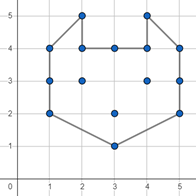
\includegraphics[width=0.7\textwidth]{pic/721.png} }
\end{minipage}
\end{figure}



---------------

Автор -- Алёна Холмогорова, М3209\question
Приведите  пример  нескольких бинарных отношений:
\begin{enumerate}
	\renewcommand{\labelenumi}{\alph{enumi})}
	\item отношение, которое является композиции нескольких бинарных отношений,  которое  обладает любым типом соответсвия  и симметрично (укажите все бинарные отношения, участвующие в композиции)
	\item два отношения, первое -- частично упорядочивает множество, на котором оно задано и второе -- полностью упорядочивает (обязательно покажите порядок элементов множества, полученный упордочиванием бинарным отношением)
	\item отношение, такое что обратное к нему  обладает одинаковыми с ним свойствами и оба функциональны (докажите, что свойства сохранаются)
\end{enumerate}

\underline{примечание:} важно показать  множества, на которых задано бинарное отношение и доказать, что ваше бинарное отношение обладает заданными свойствами
\question
В перерыве между парами дискретной математики вы с друзьями решили зарубиться в домино. Иллюстрация ниже визуализирует данный момент игры.

\\
\begin{figure}[h]

\begin{minipage}[h]{0.55\linewidth}
\end{minipage}
\begin{minipage}[h]{0.45\linewidth}
\center{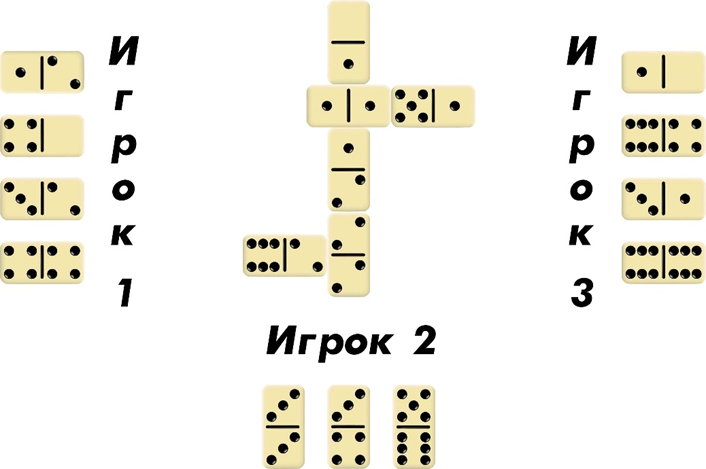
\includegraphics[width=0.7\textwidth]{pic/941.png} }
\end{minipage}
\end{figure}

Так как вы — умные студенты, вам стало интересно интерпретировать партию в виде бинарных отношений. Запишите отношения:
\begin{itemize}
    \item $G = \{(a,b)|a$ и $b$ – стороны свободных доминошек, лежащих на столе, где a – свободная сторона$\}$
    \item $R_1 = \{(a,b)|a$ и $b$ – стороны одной доминошки в руке у первого игрока$\}$
    \item $R_2 = \{(a,b)|a$ и $b$ – стороны одной доминошки в руке у второго игрока$\}$
    \item $R_3 = \{(a,b)|a$ и $b$ – стороны одной доминошки в руке у третьего игрока$\}$
\end{itemize}

Используя операцию композиции, составьте новые бинарные отношения:
\begin{itemize}
    \item $P_1$ – возможные ходы у первого игрока
    \item $P_2$ – возможные ходы у второго игрока
    \item $P_3$ – возможные ходы у третьего игрока
\end{itemize}


Ходом является пара крайних номеров стоящих рядом доминошек.
\\
---------------

Автор -- Константин Васильев, М3213\question
Даны отношения $R_1$, $R_2$ и $R_3$ на множестве $A = \{1; 2; 3; 4; 5;\}$ 
\begin{enumerate}
	\renewcommand{\labelenumi}{\alph{enumi})}
	\item $R_1 = \{(3; 2); (3; 1); (1; 3)\}$
	\item $R_2 = \{(1; 2); (2; 2); (1; 3); (4; 5)\}$
	\item $R_3 = \{(1; 2); (2; 2); (3; 4); (3; 5); (4; 5)\}$
\end{enumerate}

\begin{enumerate}
	\renewcommand{\labelenumi}{\alph{enumi})}
	\item $R_1 \cap R_2^{-1} \cup R_3^2$
	\item $(R_1 \cup R_2) \cap R_3$
	\item $R_3^2 \cap R_3^{-1}$
	\item $R_3^{-1} \cup \overline{R_2^{-1}}$
	\item $R_1^{-1} \cup \overline{R_2} \cup R_3$
\end{enumerate}

определите основные свойства, получившихся отношений
определите какие свойства сохраняются относительно исходных отношений $R_1$, $R_2$ и $R_3$ 

\underline{примечание:} результатом может быть пустое множество

\end{questions}
\newpage
%%% begin test
\begin{flushright}
\begin{tabular}{p{2.8in} r l}
%\textbf{\class} & \textbf{ФИО:} & \makebox[2.5in]{\hrulefill}\\
\textbf{\class} & \textbf{ФИО:} &Корчагинс Данила
\\

\textbf{\examdate} &&\\
%\textbf{Time Limit: \timelimit} & Teaching Assistant & \makebox[2in]{\hrulefill}
\end{tabular}\\
\end{flushright}
\rule[1ex]{\textwidth}{.1pt}


\begin{questions}
\question
В самом мирном городе мира, Лос-Сантосе, орудуют несколько бандитских группировок: Гроув-стрит, Баллос и Вагос. Некоторые районы города, для удобства бандитов помеченные цифрами \{0...9\}, находятся под влиянием этих банд:
\begin{itemize}
    \item Гроув-стрит: \{1, 2, 3, 7, 9\}
    \item Баллос: \{1, 3, 7, 8\}
    \item Вагос: \{4, 6, 7, 9\}
\end{itemize}
Районы, оказавшиеся под влиянием нескольких банд, называются спорными территориями.
\\
\\
В один прекрасный летний день Си-Джей увидел на стене своего дома граффити с сообщением от информатора из банды Баллосов. Для конспирации он оставил его в таком виде:
\begin{equation*}
B \cap \overline{G} \cup G \cap V \cap \overline{B} \cup G \cap B \cap \overline{V}
\end{equation*}
В нем содержатся номера районов, на которые полиция планирует совершить облаву. Вам, как самому умному представителю Гроув-Стрит, необходимо расшифровать граффити, а затем ответить на следующие вопросы:

\begin{itemize}
    \item Какие районы являются спорными территориями, под влиянием двух или трех банд?
    \item Какие районы полностью находятся под влиянием банды Вагос, без участия других банд?
    \item На какие из районов полиция не планирует совершать облаву?
\end{itemize}

---------------

Автор -- Константин Васильев, М3213\question
Упростите следующее выражение с учетом того, что $A\subset B \subset C \subset D \subset U; A \neq \emptyset$
\begin{equation*}
	\overline{A} \cap \overline{B} \cup B \cap \overline{C} \cup \overline{C} \cap D
\end{equation*}

Примечание: $U$ -- универсум\question
Укажите номера множеств, являющихся подмножествами множества
\begin{equation*}
	Q = \bar{A} \cap B \cup A \cap \bar{B} \cup A \cap \bar{C} \cup \bar{A} \cap C \cap \bar{D}
\end{equation*}

\begin{enumerate}
	\renewcommand{\labelenumi}{\arabic{enumi})}
	\item $P = A \cap \bar{B} \cap D \cup \bar{A} \cap \bar{B} \cap C$;
	\item $P = A \cap B \cap D \cup \bar{A} \cap \bar{C} \cap D$;
	\item $P = B \cap \bar{C} \cap \bar{D} \cup A \cap B \cap \bar{C}$;
	\item $P = A \cap \bar{C} \cap \bar{D} \cup \bar{A} \cap \bar{B} \cap D$.
\end{enumerate}
\question
Постройте разбиения множеств:
\begin{enumerate}
	\renewcommand{\labelenumi}{\alph{enumi})}
	\item $A = \{6, 7, 8, 9, 11, 14, 34, 54, 47, 18, 91, 55, 65, 76, 28, 19\};$
	\item $B = \{0, 11, 22, 33, 44, 55, 65, 76, 28, 19\}$
	\item $A \cup B$
\end{enumerate}
Таким образом, чтобы все разбиения имели как минимум 2 одинаковых множества в разбиениях.
Мощность каждого разбиение была более 3.
Докажите, что ваш ответ соответствует указанным условиям!
\question
Пусть у нас есть $P$ -- множество студентов города Санкт-Петербург, из них $A$ -- третьекурсники, $B$ -- проходят профессиональную переподготовку, а $C$ -- стажируются в Яндексе. Для статьи “Как учиться на третьем курсе университета ИТМО, проходить профессиональную подготовку и не умереть” Мегабайт создал выборку $D$.
\\
\\
Упростите множество $E = (P \cap D \cup C \cap \overline{B} \cap \overline{D} \cup B \cap A \cap \overline{C}) \cap \overline{C} \cap \overline{D} \cap P$, а затем опишите его словами.
\\
\\
---------------

Автор -- Антонина Чернова, М33081\question
Дано отношение на множестве $\{1, 2, 3, 4, 5\}$ 
\begin{equation*}
	aRb \iff b > a
\end{equation*}

(ЧАСТЬ 1) Какими основным свойствами обладает отношение? (Дайте обоснованный ответ по всем пунктам ниже: докажите наличие или отсутствие свойств)  
\begin{enumerate}
	\renewcommand{\labelenumi}{\alph{enumi})}
	\item рефлексивность / антирефлексивность / нерефлексивность
	\item симметричность / антисимметричность / асимметричность / несимметричность
	\item транзитивность / антитранзитивность / нетранзитивность
\end{enumerate}

(ЧАСТЬ 2) Обоснуйте свой ответ по каждому из приведенных ниже вопросов:
\begin{enumerate}
	\renewcommand{\labelenumi}{\alph{enumi})}
    \item Является ли это отношение отношением эквивалентности?
    \item Является ли это отношение функциональным?
    \item Каким из отношений соответствия (одно-многозначным, много-многозначный и т.д.) оно является?
    \item К каким из отношений порядка (строгого, не строгого и т.д.) можно отнести данное отношение?
\end{enumerate}
\question
Одним теплым вечером кот Степан вдохновился картинами, которые он увидел в Эрмитаже, и решил нарисовать свой автопортрет. Так как у Степана была тетрадка в клетку, оставшаяся после пройденного курса дискретной математики, он решил рисовать там. Нарисовав автопортрет ровно по клеткам, он подумал, что можно дорисовать координатные оси и обозначить все целые точки, пересекающиеся с контуром портрета. На обратной стороне листка он увидел конспект лекции по бинарным отношениям. Но так как память у кота не очень хорошая, он решил попросить вас найти бинарное отношение, соответствующее рисунку и два таких бинарных отношения, чтобы в композиции они давали исходное бинарное отношение и изобразить их.
\\
\begin{figure}[h]

\begin{minipage}[h]{0.55\linewidth}
\end{minipage}
\begin{minipage}[h]{0.45\linewidth}
\center{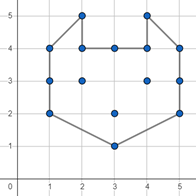
\includegraphics[width=0.7\textwidth]{pic/721.png} }
\end{minipage}
\end{figure}



---------------

Автор -- Алёна Холмогорова, М3209\question
Пусть $A = \{a, b, c, 1, \Delta\}$. Рассмотрим следующее отношение R:

\begin{equation*}
R = \{(a, a), (b, b), (c, c), (1, 1),
(\Delta, \Delta), (a, b), (b, 1), (a, 1),
(a, \Delta), (b, \Delta), (a, c), (c, \Delta)\}
\end{equation*}
\begin{itemize}
    \item Докажите, что R -- отношение порядка.
    \item У каких из следующих множеств есть наибольший/наименьший элемент?
    \begin{itemize}
        \item $X_1 = \{b, 1, \Delta\}$
        \item $X_2 = \{b, c, \Delta\}$
        \item $X_3 = \{1, c, \Delta\}$
        \item $X_4 = \{a, b, c, \Delta\}$
        \item $X_5 = \{1, c\}$
        \item $X_6 = \{ \Delta \}$
        \item $X_7 = \{b, c\}$
    \end{itemize}
    \item Полностью или частично упорядочите множество А.
\end{itemize}
\\
---------------

Автор -- Алексей Ващенков, М3205\question
Довольные студенты ИТМО сдали летнюю сессию и намерены поехать домой на некоторое время. К сожалению, чтобы добраться до пункта назначения, им потребуется сделать несколько пересадок.

Пусть множество всех населенных пунктов выглядит как: $A = \{1, 2, 3, 4, 5, 6\}$.
\\
Тогда $R = \{(1, 3), (3, 1), (2, 4), (4, 2), (1, 5), (5, 1), (2, 3), (3, 2)\}$ -- можно доехать на автобусе, $S = \{(5, 6), (6, 5), (3, 6), (6, 3)\}$ -- можно долететь на самолете.

\begin{itemize}
    \item Найдите такие пары пунктов, для перемещения между которыми надо проехать на автобусе, а затем воспользоваться самолетом и наоборот.
    \item Найдите пары пунктов, между которыми можно перемещаться на автобусе с одной пересадкой (пары вида (1, 1) не стоит указывать в ответе).
    \item Найдите пары пунктов, между которыми можно перемещаться на самолете с одной пересадкой в промежуточном пункте.
\end{itemize}
\\
---------------

Автор -- Елизавета Котельникова, М3212\question
Даны отношения $R_1$, $R_2$ и $R_3$ на множестве $A = \{1; 2; 3; 4; 5;\}$ 
\begin{enumerate}
	\renewcommand{\labelenumi}{\alph{enumi})}
	\item $R_1 = \{(3; 2); (3; 1); (1; 3)\}$
	\item $R_2 = \{(1; 2); (2; 2); (1; 3); (1; 5); (2; 3); (4; 5)\}$
	\item $R_2 = \{(1; 2); (2; 2); (3; 4); (3; 5); (4; 5)\}$
\end{enumerate}

\begin{enumerate}
	\renewcommand{\labelenumi}{\alph{enumi})}
	\item $R_1 \cap R_2$
	\item $(R_1 \cup R_2) \cap R_3$
	\item $R_3^2 \cap R_3^{-1}$
	\item $R_3 \cup \overline{R_2^2}$
	\item $R_1 \cup \overline{R_2} \cup R_3$
\end{enumerate}

определите основные свойства, получившихся отношений
определите какие свойства сохраняются относительно исходных отношений $R_1$, $R_2$ и $R_3$ 

\underline{примечание:} результатом может быть пустое множество

\end{questions}
\newpage
%%% begin test
\begin{flushright}
\begin{tabular}{p{2.8in} r l}
%\textbf{\class} & \textbf{ФИО:} & \makebox[2.5in]{\hrulefill}\\
\textbf{\class} & \textbf{ФИО:} &Кочкин Тарас Сергеевич
\\

\textbf{\examdate} &&\\
%\textbf{Time Limit: \timelimit} & Teaching Assistant & \makebox[2in]{\hrulefill}
\end{tabular}\\
\end{flushright}
\rule[1ex]{\textwidth}{.1pt}


\begin{questions}
\question
В университете MIT(O) для удобства работы с цифровыми данными у каждого студента есть свой уникальный идентификационный номер ИСУ: \{1, 2, 3… 9\}. В вузе есть различные клубы из студентов:
\begin{itemize}
    \item клуб любителей мат. анализа (обознач. буквой $M$), состоит из студентов: \{1, 2, 5, 6\}
    \item клуб любителей лин. алгебры (обознач. буквой $L$), состоит из студентов: \{1, 7, 5, 9, 4\}
    \item клуб любителей алгоритмов (обознач. буквой $A$), состоит из студентов: \{2, 8, 3, 1\}
    \item клуб любителей программирования (обознач. буквой $P$), состоит из студентов: \{1, 2, 6, 3, 8, 9\}
\end{itemize}
Студент Вася очень любит ДМ, и поэтому он захотел создать клуб любителей дискретной математики. Для создания клуба необходимо отправить письмо в студ. офис, указав там список участников. Но Вася решил продемонстрировать свои знания дискретки, и отправил вместо списка эту записку:
\begin{center}
"множество участников клуба -- это $X$, где $M \cap A \cup M \cap P \cap A \cup (L \cap (\overline{L} \cup P))$"
\end{center}
\\
Помогите студ. офису составить список участников клуба, упростив выражение Васи.

---------------

Автор -- Тимур Гонтарь, М3206\question
Упростите следующее выражение с учетом того, что $A\subset B \subset C \subset D \subset U; A \neq \emptyset$
\begin{equation*}
	A \cap B \cup \overline{A} \cap \overline{C} \cup A \cap C \cup \overline{B} \cap \overline{C}
\end{equation*}

Примечание: $U$ -- универсум\question
Укажите номера множеств, являющихся подмножествами множества
\begin{equation*}
	Q = \bar{A} \cap C \cup A \cap \bar{B} \cup A \cap \bar{C} \cup \bar{A} \cap B \cap D
\end{equation*}

\begin{enumerate}
	\renewcommand{\labelenumi}{\arabic{enumi})}
	\item $P = A \cap \bar{B} \cap D \cup \bar{A} \cap \bar{B} \cap C$;
	\item $P = A \cap B \cap D \cup \bar{A} \cap \bar{C} \cap D$;
	\item $P = B \cap \bar{C} \cap \bar{D} \cup A \cap B \cap \bar{C}$;
	\item $P = A \cap \bar{C} \cap \bar{D} \cup \bar{A} \cap \bar{B} \cap D$.
\end{enumerate}
\question
Постройте разбиения множеств:
\begin{enumerate}
	\renewcommand{\labelenumi}{\alph{enumi})}
	\item $A = \{6, 7, 8, 9, 11, 14, 34, 54, 47, 18, 91, 55, 65, 76, 28, 19\};$
	\item $B = \{0, 11, 14, 34, 22, 33, 44, 55, 65, 76, 28, 19\}$
	\item $A \cup B$
	\item $A \cap B$
\end{enumerate}
Таким образом, чтобы все разбиения имели как минимум 2 одинаковых множества в разбиениях.
Мощность каждого разбиение была более 5.
Докажите, что ваш ответ соответствует указанным условиям!
\question
Докажите, что два выражения равны.

\begin{equation}
    (A \cup B) \backslash C = (A \backslash C) \cup (B \backslash C)
\end{equation}

\begin{equation}
    (A \backslash B) \cap C = (A \cap C) \backslash (B \cap C)
\end{equation}

\begin{equation}
    A \times (B \cap C) = (A \times B) \cap (A \times C)
\end{equation}

\begin{equation}
    A \times (B \cup C) = (A \times B) \cup (A \times C)
\end{equation}
\\
\\
$\times$ -- декартово произведение
\\
---------------

Автор -- Алексей Лёвушкин, М3204\question
Бабушка Люда потеряла книгу со своими лучшими рецептами напитков. Вы, как добросовестный внук, проводивший у любимой бабушки большое количество времени, помните из чего бабуля варила вкуснейшие морсы и компоты. Обычно бабушка варила напитки из двух видов ягод и фруктов среди которых были: Малина, Облепиха, Жимолость, Смородина, Яблоки, Абрикосы и Груши. Также вы помните, что нельзя совмещать между собой Облепиху и красные ягоды, Абрикос и ягоды, Яблоко и ягоды. Постройте бинарное отношение содержащее все возможные сочетания для напитков таким образом, чтобы ингредиенты не повторялись.
\\
Ответьте на вопросы касаемо построенного бинарного отношения:
\begin{itemize}
    \item Какими свойствами обладает данное БО? Обоснуйте
    \item Является ли данное отношение функциональным?
    \item Каким из отношений соответствия оно является? (одно-многозначным, много-многозначным и т.д.)
\end{itemize}
\\
---------------

Автор -- Максим Акимцов, М3208\question
Одним теплым вечером кот Степан вдохновился картинами, которые он увидел в Эрмитаже, и решил нарисовать свой автопортрет. Так как у Степана была тетрадка в клетку, оставшаяся после пройденного курса дискретной математики, он решил рисовать там. Нарисовав автопортрет ровно по клеткам, он подумал, что можно дорисовать координатные оси и обозначить все целые точки, пересекающиеся с контуром портрета. На обратной стороне листка он увидел конспект лекции по бинарным отношениям. Но так как память у кота не очень хорошая, он решил попросить вас найти бинарное отношение, соответствующее рисунку и два таких бинарных отношения, чтобы в композиции они давали исходное бинарное отношение и изобразить их.
\\
\begin{figure}[h]

\begin{minipage}[h]{0.55\linewidth}
\end{minipage}
\begin{minipage}[h]{0.45\linewidth}
\center{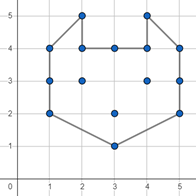
\includegraphics[width=0.7\textwidth]{pic/721.png} }
\end{minipage}
\end{figure}



---------------

Автор -- Алёна Холмогорова, М3209\question
Приведите  пример  нескольких бинарных отношений:
\begin{enumerate}
	\renewcommand{\labelenumi}{\alph{enumi})}
	\item отношение, которое является композиции нескольких бинарных отношений,  которое  обладает любым типом соответсвия  и симметрично (укажите все бинарные отношения, участвующие в композиции)
	\item два отношения, первое -- частично упорядочивает множество, на котором оно задано и второе -- полностью упорядочивает (обязательно покажите порядок элементов множества, полученный упордочиванием бинарным отношением)
	\item отношение, такое что обратное к нему  обладает одинаковыми с ним свойствами и оба функциональны (докажите, что свойства сохранаются)
\end{enumerate}

\underline{примечание:} важно показать  множества, на которых задано бинарное отношение и доказать, что ваше бинарное отношение обладает заданными свойствами
\question
Довольные студенты ИТМО сдали летнюю сессию и намерены поехать домой на некоторое время. К сожалению, чтобы добраться до пункта назначения, им потребуется сделать несколько пересадок.

Пусть множество всех населенных пунктов выглядит как: $A = \{1, 2, 3, 4, 5, 6\}$.
\\
Тогда $R = \{(1, 3), (3, 1), (2, 4), (4, 2), (1, 5), (5, 1), (2, 3), (3, 2)\}$ -- можно доехать на автобусе, $S = \{(5, 6), (6, 5), (3, 6), (6, 3)\}$ -- можно долететь на самолете.

\begin{itemize}
    \item Найдите такие пары пунктов, для перемещения между которыми надо проехать на автобусе, а затем воспользоваться самолетом и наоборот.
    \item Найдите пары пунктов, между которыми можно перемещаться на автобусе с одной пересадкой (пары вида (1, 1) не стоит указывать в ответе).
    \item Найдите пары пунктов, между которыми можно перемещаться на самолете с одной пересадкой в промежуточном пункте.
\end{itemize}
\\
---------------

Автор -- Елизавета Котельникова, М3212\question
Даны отношения $R_1$, $R_2$ и $R_3$ на множестве $A = \{1; 2; 3; 4; 5;\}$ 
\begin{enumerate}
	\renewcommand{\labelenumi}{\alph{enumi})}
	\item $R_1 = \{(1; 1); (2; 2); (3; 3); (2; 1);\}$
	\item $R_2 = \{(1; 2); (3; 4); (3; 5); (4; 5)\}$
	\item $R_2 = \{(1; 3); (1; 5); (3; 4); (4; 5)\}$
\end{enumerate}

\begin{enumerate}
	\renewcommand{\labelenumi}{\alph{enumi})}
	\item $(R_1 \cap R_2) \cup R_3$
	\item $R_1 \cup R_3$
	\item $R_1^3 \cap R_3^{-1}$
	\item $R_3 \cup R_2^2$
	\item $R_2 \cup \overline{R_1}$
\end{enumerate}

определите основные свойства, получившихся отношений
определите какие свойства сохраняются относительно исходных отношений $R_1$, $R_2$ и $R_3$

\underline{примечание:} результатом может быть пустое множество

\end{questions}
\newpage
%%% begin test
\begin{flushright}
\begin{tabular}{p{2.8in} r l}
%\textbf{\class} & \textbf{ФИО:} & \makebox[2.5in]{\hrulefill}\\
\textbf{\class} & \textbf{ФИО:} &Матюхин Алексей Александрович
\\

\textbf{\examdate} &&\\
%\textbf{Time Limit: \timelimit} & Teaching Assistant & \makebox[2in]{\hrulefill}
\end{tabular}\\
\end{flushright}
\rule[1ex]{\textwidth}{.1pt}


\begin{questions}
\question
Вы -- великая искательница сокровищ Лариса Крафтовое. Очередное путешествие забросило вас в подземные гробницы Сигизмунда I. К сожалению, на вашем пути встал очень назойливый мраморный привратник, который по всем канонам жанра имеет для вас пару загадок.
\\
\\
Привратник загадывает свое множество $X$, а также дает вам парочку других $(A,B,C…)$, объединяя, пересекая, дополняя и/или выполняя разность над которыми вы должны получить его множество. Загвоздка лишь в том, что привратник сам выбирает расстановку множеств в формуле, поэтому вам остается лишь вставить операции и расставить скобки (при надобности).

\paragraph{Загадка 1:}
\begin{equation*}
    X=\{1,2,5,6\}
\end{equation*}
\begin{equation*}
    A=\{1,2,3,4\}; B=\{2,3,4,5\}; C=\{2,5\}; D=\{4,5,6\}
    \end{equation*}
\begin{equation*}
    A ? B ? C ? D = X
\end{equation*}

\paragraph{Загадка 2:}
\begin{equation*}
    X=\{3,4,5\}
\end{equation*}
\begin{equation*}
    A=\{2,3,4,5\}; B=\{1,2,3\}; C=\{3,4,5\}; D=\{1,5,6\}
    \end{equation*}
\begin{equation*}
    A ? B ? C ? D = X
\end{equation*}

---------------

Автор -- Константин Васильев, М3213\question
Упростите следующее выражение с учетом того, что $A\subset B \subset C \subset D \subset U; A \neq \emptyset$
\begin{equation*}
	\overline{A} \cap \overline{B} \cup B \cap \overline{C} \cup \overline{C} \cap D
\end{equation*}

Примечание: $U$ -- универсум\question
Укажите номера множеств, являющихся подмножествами множества
\begin{equation*}
	Q = \bar{A} \cap B \cup A \cap \bar{B} \cup A \cap \bar{C} \cup \bar{A} \cap C \cap \bar{D}
\end{equation*}

\begin{enumerate}
	\renewcommand{\labelenumi}{\arabic{enumi})}
	\item $P = A \cap \bar{B} \cap D \cup \bar{A} \cap \bar{B} \cap C$;
	\item $P = A \cap B \cap D \cup \bar{A} \cap \bar{C} \cap D$;
	\item $P = B \cap \bar{C} \cap \bar{D} \cup A \cap B \cap \bar{C}$;
	\item $P = A \cap \bar{C} \cap \bar{D} \cup \bar{A} \cap \bar{B} \cap D$.
\end{enumerate}
\question
Постройте разбиения множеств:
\begin{enumerate}
	\renewcommand{\labelenumi}{\alph{enumi})}
	\item $A = \{6, 7, 8, 9, 11, 14, 34, 54, 47, 18, 91, 55, 65, 76, 28, 19\};$
	\item $B = \{0, 11, 22, 33, 44, 55, 65, 76, 28, 19\}$
	\item $A \cup B$
\end{enumerate}
Таким образом, чтобы все разбиения имели как минимум 2 одинаковых множества в разбиениях.
Мощность каждого разбиение была более 3.
Докажите, что ваш ответ соответствует указанным условиям!
\question
Упростить выражения, используя свойства операций над множествами:

\begin{enumerate}
	\renewcommand{\labelenumi}{\alph{enumi})}
	\item $(A\cap B \cap C \cap D) \cup (\overline{\overline{A}\cup C}\cap D) \cup (D\cap\overline{(\overline{A}+C)+D})\cup (\overline{A}\cap B\cap C \cap D)$;
	\item $(A\cap B \cap C \cap D \cap (A\cup D \cup \overline{A\cap D}))\cup \overline{\overline{A}\cup \overline{D}\cup C\cup D}\cup (A\cap B \cap (D\cap\overline{C}\cup C\cap\overline{D}))$.
\end{enumerate}
\question
Дано отношение на множестве $\{1, 2, 3, 4, 5\}$ 
\begin{equation*}
	aRb \iff a \leqslant b
\end{equation*}

(ЧАСТЬ 1) Какими основным свойствами обладает отношение? (Дайте обоснованный ответ по всем пунктам ниже: докажите наличие или отсутствие свойств)  
\begin{enumerate}
	\renewcommand{\labelenumi}{\alph{enumi})}
	\item рефлексивность / антирефлексивность / нерефлексивность
	\item симметричность / антисимметричность / асимметричность / несимметричность
	\item транзитивность / антитранзитивность / нетранзитивность
\end{enumerate}

(ЧАСТЬ 2) Обоснуйте свой ответ по каждому из приведенных ниже вопросов:
\begin{enumerate}
	\renewcommand{\labelenumi}{\alph{enumi})}
    \item Является ли это отношение отношением эквивалентности?
    \item Является ли это отношение функциональным?
    \item Каким из отношений соответствия (одно-многозначным, много-многозначный и т.д.) оно является?
    \item К каким из отношений порядка (строгого, не строгого и т.д.) можно отнести данное отношение?
\end{enumerate}
\question
Приведите доказательства следующих утверждений:
\begin{itemize}
    \item Доказать, что отношение «равенство по модулю 5» является отношением эквивалентности на множестве целых чисел.
    \item Докажите, что всякое отношение строгого порядка является асимметричным.
    \item R задано на декартовом квадрате натуральных чисел. Пара $(m,n)$ принадлежит отношению $R$, если $n^3 + 3m^2 + 2m$ делится на 6. Докажите, что это - отношение эквивалентности.
\end{itemize}
\\
---------------

Автор -- разные студенты потока ИС2026\question
Приведите  пример  нескольких бинарных отношений:
\begin{enumerate}
	\renewcommand{\labelenumi}{\alph{enumi})}
	\item отношение, которое является композиции нескольких бинарных отношений,  которое  нестрого порядка  и антисимметрично (укажите все бинарные отношения, участвующие в композиции)
	\item отношение, которое частично упорядочивает множество и как минимум 7 элементов упорядочены (обязательно покажите порядок элементов множества, полученный упордочиванием бинарным отношением)
	\item отношение, такое что обратное к нему  обладает одинаковыми с ним свойствами и оба антирефлексивны и симметричны (докажите, что свойства сохранаются)
\end{enumerate}

\underline{примечание:} важно показать  множества, на которых задано бинарное отношение и доказать, что ваше бинарное отношение обладает заданными свойствами
\question
В перерыве между парами дискретной математики вы с друзьями решили зарубиться в домино. Иллюстрация ниже визуализирует данный момент игры.

\\
\begin{figure}[h]

\begin{minipage}[h]{0.55\linewidth}
\end{minipage}
\begin{minipage}[h]{0.45\linewidth}
\center{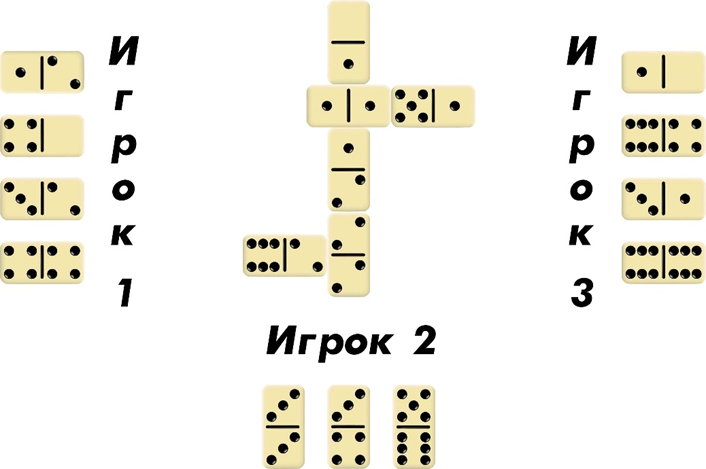
\includegraphics[width=0.7\textwidth]{pic/941.png} }
\end{minipage}
\end{figure}

Так как вы — умные студенты, вам стало интересно интерпретировать партию в виде бинарных отношений. Запишите отношения:
\begin{itemize}
    \item $G = \{(a,b)|a$ и $b$ – стороны свободных доминошек, лежащих на столе, где a – свободная сторона$\}$
    \item $R_1 = \{(a,b)|a$ и $b$ – стороны одной доминошки в руке у первого игрока$\}$
    \item $R_2 = \{(a,b)|a$ и $b$ – стороны одной доминошки в руке у второго игрока$\}$
    \item $R_3 = \{(a,b)|a$ и $b$ – стороны одной доминошки в руке у третьего игрока$\}$
\end{itemize}

Используя операцию композиции, составьте новые бинарные отношения:
\begin{itemize}
    \item $P_1$ – возможные ходы у первого игрока
    \item $P_2$ – возможные ходы у второго игрока
    \item $P_3$ – возможные ходы у третьего игрока
\end{itemize}


Ходом является пара крайних номеров стоящих рядом доминошек.
\\
---------------

Автор -- Константин Васильев, М3213\question
Даны отношения $R_1$, $R_2$ и $R_3$ на множестве $A = \{1; 2; 3; 4; 5;\}$ 
\begin{enumerate}
	\renewcommand{\labelenumi}{\alph{enumi})}
	\item $R_1 = \{(2; 1); (1; 2); (2; 3); (3; 2); (3; 1); (1; 3)\}$
	\item $R_2 = \{(1; 2); (2; 2); (1; 3); (1; 5); (2; 3); (2; 4); (2; 5); (4; 5)\}$
	\item $R_3 = \{(1; 2); (2; 2); (1; 3); (1; 5); (3; 4); (3; 5); (4; 5)\}$
\end{enumerate}

\begin{enumerate}
	\renewcommand{\labelenumi}{\alph{enumi})}
	\item $\overline{R_1} \cap R_2^{-1} \cap R_3$
	\item $(R_1^3 \cup R_2) \cap R_3^{-1}$
	\item $R_3 \cap R_3^{-1}$
	\item $R_3^{-1} \cup \overline{R_2^{-1}}$
	\item $R_1^{-1} \cup \overline{R_2} \cup R_3$
\end{enumerate}

определите основные свойства, получившихся отношений
определите какие свойства сохраняются относительно исходных отношений $R_1$, $R_2$ и $R_3$ 

\underline{примечание:} результатом может быть пустое множество

\end{questions}
\newpage
%%% begin test
\begin{flushright}
\begin{tabular}{p{2.8in} r l}
%\textbf{\class} & \textbf{ФИО:} & \makebox[2.5in]{\hrulefill}\\
\textbf{\class} & \textbf{ФИО:} &Миняев Никита
\\

\textbf{\examdate} &&\\
%\textbf{Time Limit: \timelimit} & Teaching Assistant & \makebox[2in]{\hrulefill}
\end{tabular}\\
\end{flushright}
\rule[1ex]{\textwidth}{.1pt}


\begin{questions}
\question
В самом мирном городе мира, Лос-Сантосе, орудуют несколько бандитских группировок: Гроув-стрит, Баллос и Вагос. Некоторые районы города, для удобства бандитов помеченные цифрами \{0...9\}, находятся под влиянием этих банд:
\begin{itemize}
    \item Гроув-стрит: \{1, 2, 3, 7, 9\}
    \item Баллос: \{1, 3, 7, 8\}
    \item Вагос: \{4, 6, 7, 9\}
\end{itemize}
Районы, оказавшиеся под влиянием нескольких банд, называются спорными территориями.
\\
\\
В один прекрасный летний день Си-Джей увидел на стене своего дома граффити с сообщением от информатора из банды Баллосов. Для конспирации он оставил его в таком виде:
\begin{equation*}
B \cap \overline{G} \cup G \cap V \cap \overline{B} \cup G \cap B \cap \overline{V}
\end{equation*}
В нем содержатся номера районов, на которые полиция планирует совершить облаву. Вам, как самому умному представителю Гроув-Стрит, необходимо расшифровать граффити, а затем ответить на следующие вопросы:

\begin{itemize}
    \item Какие районы не под контролем ни одной из этих банд?
    \item Какое количество районов охватывают все три банды?
    \item На какие из районов, находящихся под вашим влиянием, будет совершена облава?
\end{itemize}

---------------

Автор -- Константин Васильев, М3213\question
Упростите следующее выражение с учетом того, что $A\subset B \subset C \subset D \subset U; A \neq \emptyset$
\begin{equation*}
	\overline{A} \cap \overline{C} \cap D \cup \overline{B} \cap \overline{C} \cap D \cup A \cap B
\end{equation*}

Примечание: $U$ -- универсум\question
Укажите номера множеств, являющихся подмножествами множества
\begin{equation*}
	Q = A \cap \bar{D} \cup B \cap C \cup \bar{A} \cap \bar{B} \cap D \cup A \cap C
\end{equation*}

\begin{enumerate}
	\renewcommand{\labelenumi}{\arabic{enumi})}
	\item $P = B \cap C \cap D \cup \bar{A} \cap B \cap C$;
	\item $P = \bar{B} \cap \bar{C} \cap D \cup B \cap \bar{C} \cap \bar{D}$;
	\item $P = A \cap \bar{B} \cap D \cup A \cap C \cap D$;
	\item $P = \bar{B} \cap \bar{C} \cup \bar{A} \cap \bar{B} \cap D$.
\end{enumerate}
\question
Постройте разбиения множеств:
\begin{enumerate}
	\renewcommand{\labelenumi}{\alph{enumi})}
	\item $A = \{6, 7, 8, 9, 11, 14, 34, 54, 47, 18, 91, 55, 65, 76, 28, 19\};$
	\item $B = \{0, 11, 14, 34, 22, 33, 44, 55, 65, 76, 28, 19\}$
	\item $A \cup B$
	\item $A \cap B$
\end{enumerate}
Таким образом, чтобы все разбиения имели как минимум 2 одинаковых множества в разбиениях.
Мощность каждого разбиение была более 5.
Докажите, что ваш ответ соответствует указанным условиям!
\question
Пусть у нас есть $P$ -- множество студентов города Санкт-Петербург, из них $A$ -- третьекурсники, $B$ -- проходят профессиональную переподготовку, а $C$ -- стажируются в Яндексе. Для статьи “Как учиться на третьем курсе университета ИТМО, проходить профессиональную подготовку и не умереть” Мегабайт создал выборку $D$.
\\
\\
Упростите множество $E = (P \cap D \cup C \cap \overline{B} \cap \overline{D} \cup B \cap A \cap \overline{C}) \cap \overline{C} \cap \overline{D} \cap P$, а затем опишите его словами.
\\
\\
---------------

Автор -- Антонина Чернова, М33081\question
Довольные студенты ИТМО сдали летнюю сессию и намерены поехать домой на некоторое время. К сожалению, чтобы добраться до пункта назначения, им потребуется сделать несколько пересадок.

Пусть множество всех населенных пунктов выглядит как: $A = \{1, 2, 3, 4, 5, 6\}$.
\\
Тогда $R = \{(1, 3), (3, 1), (2, 4), (4, 2), (1, 5), (5, 1), (2, 3), (3, 2)\}$ -- можно доехать на автобусе, $S = \{(5, 6), (6, 5), (3, 6), (6, 3)\}$ -- можно долететь на самолете.
\\
Какими свойствами обладают отношения R и S?
\\
---------------

Автор -- Елизавета Котельникова, М3212\question
Установите, является ли каждое из перечисленных ниже отношений на А ($R \subseteq A \times A$) отношением эквивалентности (обоснование ответа обязательно). Для каждого отношения эквивалентности постройте классы 
эквивалентности и постройте граф отношения:
\begin{enumerate}
	\renewcommand{\labelenumi}{\alph{enumi})}
	\item Пусть A -- множество имен. $A = \{ $Алексей, Иван, Петр, Александр, Павел, Андрей$ \}$. Тогда отношение $R$ верно на парах имен, начинающихся с одной и той же буквы, и только на них.
	\item $A = \{-10, -9, ..., 9, 10\}$ и отношение $ R = \{(a,b)|a^{2} = b^{2}\}$
	\item На множестве $A = \{1; 2; 3\}$ задано отношение $R = \{(1; 1); (2; 2); (3; 3); (3; 2); (1; 2); (2; 1)\}$
\end{enumerate}\question
Пусть имеется бинарное отношение $R$ на $ A \times A$. Докажите, что если $R$ -- одновременно и отношение эквивалентности и отношение частичного порядка, то оно -- отношение равенства.
\\
---------------

Автор -- Алексей Ващенков, М3205\question
Два контрабандиста затеяли сделку. Им кажется, что все должно пройти гладко и их план идеален, но стражи порядка уже взялись за это дело и планируют встать между ними, сорвав аферу. $\{1, 2, 3, 0\}$ – товары, которые планирует передать контрабандист $A$. $\{1, 2, 3, 4\}$ – планирует передать $B$. $A$, ничего не подозревая, уже готов передать две штуки товара 1 в руки полицейскому (притворившегося контрабандистом $B$) в обмен на 1 и 3 товар подставного $B$, две штуки товарa 2 – тоже в обмен на 1 и 3 товар. Также полиция связалась с $B$ по поводу передачи товара 3 в обмен на 4, и 3 на 1. Таким образом, если у полиции получилось перехватить сделки с обоих концов – работа выполена, и товар не окажется в руках ни у $A$ ни у $B$. Какие и сколько сделок полиции удалось предотвратить?
\\
---------------

Автор -- Мария Баженова, М3219\question
Даны отношения $R_1$, $R_2$ и $R_3$ на множестве $A = \{1; 2; 3; 4; 5;\}$ 
\begin{enumerate}
	\renewcommand{\labelenumi}{\alph{enumi})}
	\item $R_1 = \{(3; 2); (3; 1); (1; 3)\}$
	\item $R_2 = \{(1; 2); (2; 2); (1; 3); (1; 5); (2; 3); (4; 5)\}$
	\item $R_2 = \{(1; 2); (2; 2); (3; 4); (3; 5); (4; 5)\}$
\end{enumerate}

\begin{enumerate}
	\renewcommand{\labelenumi}{\alph{enumi})}
	\item $R_1 \cap R_2$
	\item $(R_1 \cup R_2) \cap R_3$
	\item $R_3^2 \cap R_3^{-1}$
	\item $R_3 \cup \overline{R_2^2}$
	\item $R_1 \cup \overline{R_2} \cup R_3$
\end{enumerate}

определите основные свойства, получившихся отношений
определите какие свойства сохраняются относительно исходных отношений $R_1$, $R_2$ и $R_3$ 

\underline{примечание:} результатом может быть пустое множество

\end{questions}
\newpage
%%% begin test
\begin{flushright}
\begin{tabular}{p{2.8in} r l}
%\textbf{\class} & \textbf{ФИО:} & \makebox[2.5in]{\hrulefill}\\
\textbf{\class} & \textbf{ФИО:} &Мишуто Вадим Александрович
\\

\textbf{\examdate} &&\\
%\textbf{Time Limit: \timelimit} & Teaching Assistant & \makebox[2in]{\hrulefill}
\end{tabular}\\
\end{flushright}
\rule[1ex]{\textwidth}{.1pt}


\begin{questions}
\question
Пусть у нас есть $P$ -- множество студентов города Санкт-Петербург, из них $A$ -- третьекурсники, $B$ -- проходят профессиональную переподготовку, а $C$ -- стажируются в Яндексе. Для статьи “Как учиться на третьем курсе университета ИТМО, проходить профессиональную подготовку и не умереть” Мегабайт создал выборку $D$.

Студенты ИТМО участвуют в специальной лотерее. Мы спросили номера лотерейных билетов некоторых из них. Получилась такая статистика:

\begin{center}
$A = \{1, 3, 7, 12, 15, 19, 22\}$
\\
$B = \{2, 3, 7, 9, 13, 16, 18, 21, 24\}$
\\
$C = \{2, 4, 5, 8, 10, 11, 13, 14, 17, 21, 23\}$
\\
$D = \{1, 2, 9, 13, 16, 19, 21, 22, 24\}$
\end{center}

Помогите Мегабайту понять, какие номера билетов у студентов из их выборки, которые стажируются в Яндексе.

---------------

Автор -- Антонина Чернова, М33081\question
Упростите следующее выражение с учетом того, что $A\subset B \subset C \subset D \subset U; A \neq \emptyset$
\begin{equation*}
	A \cap C  \cap D \cup B \cap \overline{C} \cap D \cup B \cap C \cap D
\end{equation*}

Примечание: $U$ -- универсум\question
Укажите номера множеств, являющихся подмножествами множества
\begin{equation*}
	Q = \bar{A} \cup B \cap C \cup \bar{C} \cap \bar{D}
\end{equation*}

\begin{enumerate}
	\renewcommand{\labelenumi}{\arabic{enumi})}
	\item $P = A \cap \bar{B} \cap D \cup \bar{A} \cap \bar{B} \cap C$;
	\item $P = A \cap B \cap D \cup \bar{A} \cap \bar{C} \cap D$;
	\item $P = B \cap \bar{C} \cap \bar{D} \cup A \cap B \cap \bar{C}$;
	\item $P = A \cap \bar{C} \cap \bar{D} \cup \bar{A} \cap \bar{B} \cap D$.
\end{enumerate}
\question
Постройте разбиения множеств:
\begin{enumerate}
	\renewcommand{\labelenumi}{\alph{enumi})}
	\item $A = \{6, 7, 8, 9, 11, 14, 34, 54, 47, 18, 91, 55, 65, 76, 28, 19\};$
	\item $B = \{0, 11, 14, 34, 22, 33, 44, 55, 65, 76, 28, 19\}$
	\item $A \cup B$
	\item $A \cap B$
\end{enumerate}
Таким образом, чтобы все разбиения имели как минимум 2 одинаковых множества в разбиениях.
Мощность каждого разбиение была более 5.
Докажите, что ваш ответ соответствует указанным условиям!
\question
Докажите, что два выражения равны.

\begin{equation}
    (A \cup B) \backslash C = (A \backslash C) \cup (B \backslash C)
\end{equation}

\begin{equation}
    (A \backslash B) \cap C = (A \cap C) \backslash (B \cap C)
\end{equation}

\begin{equation}
    A \times (B \cap C) = (A \times B) \cap (A \times C)
\end{equation}

\begin{equation}
    A \times (B \cup C) = (A \times B) \cup (A \times C)
\end{equation}
\\
\\
$\times$ -- декартово произведение
\\
---------------

Автор -- Алексей Лёвушкин, М3204\question
Определить и обосновать, являются ли рефлексивными/симметричными/транзитивными, отношениями порядка, одно-однозначными/одно-многозначными/много-однозначными/много-многозначными бинарные отношения:
\begin{itemize}
    \item $aRb \Leftrightarrow a$ является ребёнком $b$ ($a$ и $b$ -- люди)
    \item $aRb \Leftrightarrow a$ и $b$ живут в одной стране ($a$ и $b$ -- люди)
    \item $aRb \Leftrightarrow a$ охотится на $b$ ($a$ и $b$ -- животные)
\end{itemize}
\\
Выделите среди этих БО отношения эквивалентности и разбейте их на классы эквивалентности, продемонстрировав алгоритм разбиения.
\\
---------------

Автор -- Алексей Лёвушкин, М3204\question
Дана декартова система координат. Ось $x$ представляет собой множество $X$, ось $y$ - множество $Y$. На этих двух множествах определены бинарные отношения, которые схематически изображены в виде графиков выше (то есть, например, для графика с рис. 1 будет верно, что пары $(0, 0), (1, 1), (2, 2), (3, 3), (4, 4), (5, 5)$ входят в бинарное отношение, соответствующее графику). Для каждого из таких отношений определить:
\begin{itemize}
    \item Каким типом отношения соответствия оно является?
    \item Является ли оно функциональным отношением? Если да, то каким именно (сюръекция, инъекция, биекция)?
\end{itemize}
Обоснуйте своё решение. После этого, аналогично данным в условии графикам, придумайте отношение (любое), которое будет представлять собой полностью определенную функцию, и при этом будет инъективно и не сюръективно.
\\
\begin{figure}[h]

\begin{minipage}[h]{0.55\linewidth}
\end{minipage}
\begin{minipage}[h]{0.45\linewidth}
\center{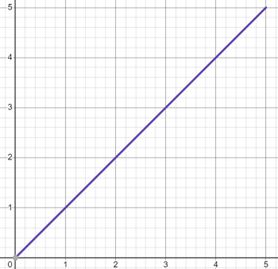
\includegraphics[width=0.7\textwidth]{pic/711.png}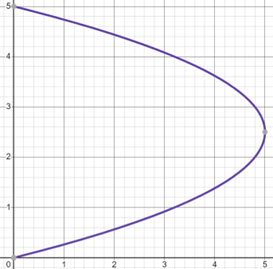
\includegraphics[width=0.7\textwidth]{pic/712.png}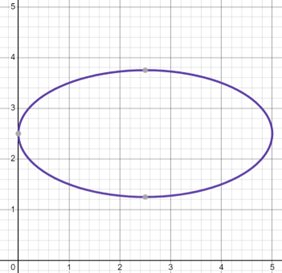
\includegraphics[width=0.7\textwidth]{pic/713.png} }
\end{minipage}
\end{figure}

---------------

Автор -- Тимур Гонтарь, М3206\question
Докажите (с подробным объяснением) или опровергните (приведя контрпример) следующие утверждения о бинарных отношениях $R \subseteq M^2$ и $S \subseteq M^2$:
\begin{itemize}
    \item Если $R$ и $S$ рефлексивны, то $R \circ S$ тоже рефлексивно.
    \item Если $R$ и $S$ симметрично, то $R \circ S$ тоже симметрично.
    \item Если $R$ и $S$ транзитивно, то $R \circ S$ тоже транзитивно.
    \item Если $R$ и $S$ рефлексивны, то $R \circ S$ тоже рефлексивно.
    \item Если $R$ и $S$ симметрично, то $R \circ S$ тоже симметрично.
    \item Если $R$ и $S$ транзитивно, то $R \circ S$ тоже транзитивно.
\end{itemize}
\\
---------------

Автор -- Алексей Лёвушкин, М3204\question
Вася хочет устроиться бэкенд разработчиком в ИТМО, работать с ИСУ. На собеседовании тимлид дал ему тестовое задание, чтобы определить его уровень знаний:
\\
\begin{figure}[h]

\begin{minipage}[h]{0.55\linewidth}
\end{minipage}
\begin{minipage}[h]{0.45\linewidth}
\center{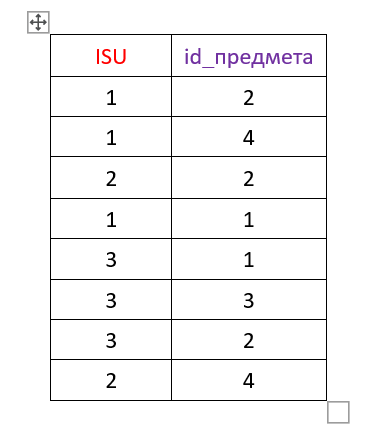
\includegraphics[width=0.7\textwidth]{pic/911.png}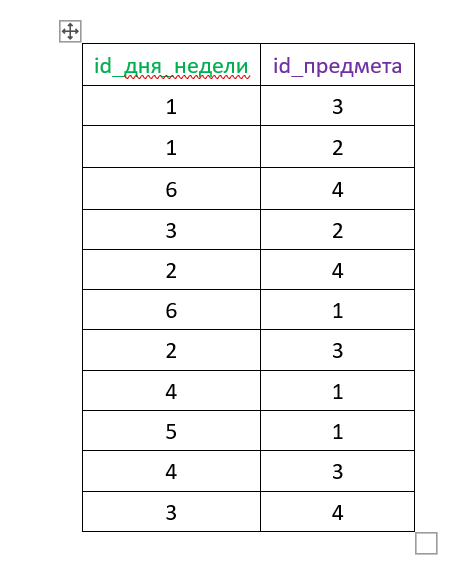
\includegraphics[width=0.7\textwidth]{pic/912.png} }
\end{minipage}
\end{figure}

В базе данных расписания ИТМО есть 2 таблицы:
\begin{itemize}
    \item В таблице 1 (рис. 1) каждому студенту по его номеру ИСУ сопоставлены предметы по их id. У одного номера ИСУ (студента) может быть много предметов, при этом на один предмет может ходить несколько студентов.
    \item В таблице 2 (рис. 2) каждому дню недели по его id (порядковый номер: 1-пн, 2-вт, 3-ср и т. д.) сопоставлены предметы по их id. В один день могут проводиться пары по нескольким предметам, при этом пары по одному предмету могут проходить несколько дней в неделе.
\end{itemize}
От Васи требуется по имеющимся данным вывести все возможные кортежи вида:

\begin{center}(номер ИСУ, день когда у этого студента есть пары)\end{center}

Например, ответ вида $\{(1, 1), (1, 5), (2, 1)\}$ будет означать что студент с ISU №1 имеет пары в понедельник и пятницу, а студент с ISU №2 имеет пары только в понедельник.

Помогите Васе решить данную задачу, используя ваши знания по дискретной математике.

---------------

Автор -- Тимур Гонтарь, М3206\question
Даны отношения $R_1$, $R_2$ и $R_3$ на множестве $A = \{1; 2; 3; 4; 5;\}$ 
\begin{enumerate}
	\renewcommand{\labelenumi}{\alph{enumi})}
	\item $R_1 = \{(3; 2); (3; 1); (1; 3)\}$
	\item $R_2 = \{(1; 2); (2; 2); (1; 3); (1; 5); (2; 3); (4; 5)\}$
	\item $R_2 = \{(1; 2); (2; 2); (3; 4); (3; 5); (4; 5)\}$
\end{enumerate}

\begin{enumerate}
	\renewcommand{\labelenumi}{\alph{enumi})}
	\item $R_1 \cap R_2$
	\item $(R_1 \cup R_2) \cap R_3$
	\item $R_3^2 \cap R_3^{-1}$
	\item $R_3 \cup \overline{R_2^2}$
	\item $R_1 \cup \overline{R_2} \cup R_3$
\end{enumerate}

определите основные свойства, получившихся отношений
определите какие свойства сохраняются относительно исходных отношений $R_1$, $R_2$ и $R_3$ 

\underline{примечание:} результатом может быть пустое множество

\end{questions}
\newpage
%%% begin test
\begin{flushright}
\begin{tabular}{p{2.8in} r l}
%\textbf{\class} & \textbf{ФИО:} & \makebox[2.5in]{\hrulefill}\\
\textbf{\class} & \textbf{ФИО:} &Полубояринов Дмитрий Павлович
\\

\textbf{\examdate} &&\\
%\textbf{Time Limit: \timelimit} & Teaching Assistant & \makebox[2in]{\hrulefill}
\end{tabular}\\
\end{flushright}
\rule[1ex]{\textwidth}{.1pt}


\begin{questions}
\question
Вы -- великая искательница сокровищ Лариса Крафтовое. Очередное путешествие забросило вас в подземные гробницы Сигизмунда I. К сожалению, на вашем пути встал очень назойливый мраморный привратник, который по всем канонам жанра имеет для вас пару загадок.
\\
\\
Привратник загадывает свое множество $X$, а также дает вам парочку других $(A,B,C…)$, объединяя, пересекая, дополняя и/или выполняя разность над которыми вы должны получить его множество. Загвоздка лишь в том, что привратник сам выбирает расстановку множеств в формуле, поэтому вам остается лишь вставить операции и расставить скобки (при надобности).

\paragraph{Загадка 1:}
\begin{equation*}
    X=\{1,2,5,6\}
\end{equation*}
\begin{equation*}
    A=\{1,2,3,4\}; B=\{2,3,4,5\}; C=\{2,5\}; D=\{4,5,6\}
    \end{equation*}
\begin{equation*}
    A ? B ? C ? D = X
\end{equation*}

\paragraph{Загадка 2:}
\begin{equation*}
    X=\{3,4,5\}
\end{equation*}
\begin{equation*}
    A=\{2,3,4,5\}; B=\{1,2,3\}; C=\{3,4,5\}; D=\{1,5,6\}
    \end{equation*}
\begin{equation*}
    A ? B ? C ? D = X
\end{equation*}

---------------

Автор -- Константин Васильев, М3213\question
Упростите следующее выражение с учетом того, что $A\subset B \subset C \subset D \subset U; A \neq \emptyset$
\begin{equation*}
	A \cap B \cup \overline{A} \cap \overline{C} \cup A \cap C \cup \overline{B} \cap \overline{C}
\end{equation*}

Примечание: $U$ -- универсум\question
Укажите номера множеств, являющихся подмножествами множества
\begin{equation*}
	Q = \bar{A} \cap C \cup A \cap \bar{B} \cup A \cap \bar{C} \cup \bar{A} \cap B \cap D
\end{equation*}

\begin{enumerate}
	\renewcommand{\labelenumi}{\arabic{enumi})}
	\item $P = B \cap C \cap D \cup \bar{A} \cap B \cap C$;
	\item $P = \bar{B} \cap \bar{C} \cap D \cup B \cap \bar{C} \cap \bar{D}$;
	\item $P = A \cap \bar{B} \cap D \cup A \cap C \cap D$;
	\item $P = \bar{B} \cap \bar{C} \cup \bar{A} \cap \bar{B} \cap D$.
\end{enumerate}
\question
Постройте разбиения множеств:
\begin{enumerate}
	\renewcommand{\labelenumi}{\alph{enumi})}
	\item $A = \{6, 7, 8, 9, 11, 14, 34, 54, 47, 18, 91\};$
	\item $B = \{0, 1, 2, 3, 4, 5, 6, 7, 8, 9\}$
	\item $A \cap B$
\end{enumerate}
Таким образом, чтобы все разбиения имели как минимум 2 одинаковых множества в разбиениях.
Мощность каждого разбиение была более 3.
Докажите, что ваш ответ соответствует указанным условиям!\question
Докажите, что два выражения равны.

\begin{equation}
    (A \cup B) \backslash C = (A \backslash C) \cup (B \backslash C)
\end{equation}

\begin{equation}
    (A \backslash B) \cap C = (A \cap C) \backslash (B \cap C)
\end{equation}

\begin{equation}
    A \times (B \cap C) = (A \times B) \cap (A \times C)
\end{equation}

\begin{equation}
    A \times (B \cup C) = (A \times B) \cup (A \times C)
\end{equation}
\\
\\
$\times$ -- декартово произведение
\\
---------------

Автор -- Алексей Лёвушкин, М3204\question
Дано отношение на множестве $\{1, 2, 3, 4, 5\}$ 
\begin{equation*}
	aRb \iff b > a
\end{equation*}

(ЧАСТЬ 1) Какими основным свойствами обладает отношение? (Дайте обоснованный ответ по всем пунктам ниже: докажите наличие или отсутствие свойств)  
\begin{enumerate}
	\renewcommand{\labelenumi}{\alph{enumi})}
	\item рефлексивность / антирефлексивность / нерефлексивность
	\item симметричность / антисимметричность / асимметричность / несимметричность
	\item транзитивность / антитранзитивность / нетранзитивность
\end{enumerate}

(ЧАСТЬ 2) Обоснуйте свой ответ по каждому из приведенных ниже вопросов:
\begin{enumerate}
	\renewcommand{\labelenumi}{\alph{enumi})}
    \item Является ли это отношение отношением эквивалентности?
    \item Является ли это отношение функциональным?
    \item Каким из отношений соответствия (одно-многозначным, много-многозначный и т.д.) оно является?
    \item К каким из отношений порядка (строгого, не строгого и т.д.) можно отнести данное отношение?
\end{enumerate}
\question
Приведите доказательства следующих утверждений:
\begin{itemize}
    \item Доказать, что отношение «равенство по модулю 5» является отношением эквивалентности на множестве целых чисел.
    \item Докажите, что всякое отношение строгого порядка является асимметричным.
    \item R задано на декартовом квадрате натуральных чисел. Пара $(m,n)$ принадлежит отношению $R$, если $n^3 + 3m^2 + 2m$ делится на 6. Докажите, что это - отношение эквивалентности.
\end{itemize}
\\
---------------

Автор -- разные студенты потока ИС2026\question
Приведите  пример  нескольких бинарных отношений:
\begin{enumerate}
	\renewcommand{\labelenumi}{\alph{enumi})}
	\item отношение, которое является композиции нескольких бинарных отношений,  которое  нестрого порядка  и антисимметрично (укажите все бинарные отношения, участвующие в композиции)
	\item отношение, которое частично упорядочивает множество и как минимум 7 элементов упорядочены (обязательно покажите порядок элементов множества, полученный упордочиванием бинарным отношением)
	\item отношение, такое что обратное к нему  обладает одинаковыми с ним свойствами и оба антирефлексивны и симметричны (докажите, что свойства сохранаются)
\end{enumerate}

\underline{примечание:} важно показать  множества, на которых задано бинарное отношение и доказать, что ваше бинарное отношение обладает заданными свойствами
\question
Даны отношения $R_1$ и $R_2$ на множестве $A = \{1; 2; 3; 4; 5\}$, постройте композиции отношений $R_1*R_2$, $R_2*R_1$,  $R_1*R_2^{-1}$, $R_1^{-1}*R_2$, $R_1^2$, $R_2^2$:
\begin{enumerate}
	\renewcommand{\labelenumi}{\alph{enumi})}
	\item $R_1 = \{(1; 1); (2; 2); (3; 3); (2; 1); (1; 2); (2; 3); (3; 2); (4; 1); (4; 5); (5; 4); (5; 5)\}$
	\item $R_2 = \{(1; 3); (2; 4); (5; 4); (1; 5); (4; 2); (2; 5)\}$
	\item задайте получившиеся отношения с помощью матриц, графов и перечислений 
	\item определите основные свойства, получившихся отношений
\end{enumerate}

\underline{примечание:} результатом может быть пустое множество
\question
Даны отношения $R_1$, $R_2$ и $R_3$ на множестве $A = \{1; 2; 3; 4; 5;\}$ 
\begin{enumerate}
	\renewcommand{\labelenumi}{\alph{enumi})}
	\item $R_1 = \{(1; 1); (2; 2); (3; 3); (2; 1);  (3; 1); (1; 3)\}$
	\item $R_2 = \{(1; 2); (2; 2); (3; 4); (3; 5); (4; 5)\}$
	\item $R_2 = \{(1; 3); (1; 5); (3; 4); (3; 5); (4; 5)\}$
\end{enumerate}

\begin{enumerate}
	\renewcommand{\labelenumi}{\alph{enumi})}
	\item $(R_1 \cap R_2) \cup R_3$
	\item $R_1 \cup R_3$
	\item $R_1^3 \cap R_3^-1$
	\item $R_3 \cup R_2^2$
	\item $R_2 \cup \overline{R_1}$
\end{enumerate}

определите основные свойства, получившихся отношений
определите какие свойства сохраняются относительно исходных отношений $R_1$, $R_2$ и $R_3$ 

\underline{примечание:} результатом может быть пустое множество

\end{questions}
\newpage
%%% begin test
\begin{flushright}
\begin{tabular}{p{2.8in} r l}
%\textbf{\class} & \textbf{ФИО:} & \makebox[2.5in]{\hrulefill}\\
\textbf{\class} & \textbf{ФИО:} &Рагулин Антон Витальевич
\\

\textbf{\examdate} &&\\
%\textbf{Time Limit: \timelimit} & Teaching Assistant & \makebox[2in]{\hrulefill}
\end{tabular}\\
\end{flushright}
\rule[1ex]{\textwidth}{.1pt}


\begin{questions}
\question
В самом мирном городе мира, Лос-Сантосе, орудуют несколько бандитских группировок: Гроув-стрит, Баллос и Вагос. Некоторые районы города, для удобства бандитов помеченные цифрами \{0...9\}, находятся под влиянием этих банд:
\begin{itemize}
    \item Гроув-стрит: \{1, 2, 3, 7, 9\}
    \item Баллос: \{1, 3, 7, 8\}
    \item Вагос: \{4, 6, 7, 9\}
\end{itemize}
Районы, оказавшиеся под влиянием нескольких банд, называются спорными территориями.
\\
\\
В один прекрасный летний день Си-Джей увидел на стене своего дома граффити с сообщением от информатора из банды Баллосов. Для конспирации он оставил его в таком виде:
\begin{equation*}
B \cap \overline{G} \cup G \cap V \cap \overline{B} \cup G \cap B \cap \overline{V}
\end{equation*}
В нем содержатся номера районов, на которые полиция планирует совершить облаву. Вам, как самому умному представителю Гроув-Стрит, необходимо расшифровать граффити, а затем ответить на следующие вопросы:

\begin{itemize}
    \item Какие районы не под контролем ни одной из этих банд?
    \item Какое количество районов охватывают все три банды?
    \item На какие из районов, находящихся под вашим влиянием, будет совершена облава?
\end{itemize}

---------------

Автор -- Константин Васильев, М3213\question
Упростите следующее выражение с учетом того, что $A\subset B \subset C \subset D \subset U; A \neq \emptyset$
\begin{equation*}
	A \cap C  \cap D \cup B \cap \overline{C} \cap D \cup B \cap C \cap D
\end{equation*}

Примечание: $U$ -- универсум\question
Укажите номера множеств, являющихся подмножествами множества
\begin{equation*}
	Q = A \cap \bar{D} \cup B \cap C \cup \bar{A} \cap \bar{B} \cap D \cup A \cap C
\end{equation*}

\begin{enumerate}
	\renewcommand{\labelenumi}{\arabic{enumi})}
	\item $P = A \cap \bar{B} \cap D \cup \bar{A} \cap \bar{B} \cap C$;
	\item $P = A \cap B \cap D \cup \bar{A} \cap \bar{C} \cap D$;
	\item $P = B \cap \bar{C} \cap \bar{D} \cup A \cap B \cap \bar{C}$;
	\item $P = A \cap \bar{C} \cap \bar{D} \cup \bar{A} \cap \bar{B} \cap D$.
\end{enumerate}
\question
Постройте разбиения множеств:
\begin{enumerate}
	\renewcommand{\labelenumi}{\alph{enumi})}
	\item $A = \{6, 7, 8, 9, 11, 14, 34, 91, 55, 65, 76, 28, 19\};$
	\item $B = \{0, 1, 2, 3, 4, 8, 9, 11, 22, 33, 44, 55, 65, 76, 28, 19\}$
	\item $A \cup B$
	\item $A \cap B$
\end{enumerate}
Таким образом, чтобы все разбиения имели как минимум 2 одинаковых множества в разбиениях.
Мощность каждого разбиение была более 4.
Докажите, что ваш ответ соответствует указанным условиям!\question
Докажите, что два выражения равны.

\begin{equation}
    (A \cup B) \backslash C = (A \backslash C) \cup (B \backslash C)
\end{equation}

\begin{equation}
    (A \backslash B) \cap C = (A \cap C) \backslash (B \cap C)
\end{equation}

\begin{equation}
    A \times (B \cap C) = (A \times B) \cap (A \times C)
\end{equation}

\begin{equation}
    A \times (B \cup C) = (A \times B) \cup (A \times C)
\end{equation}
\\
\\
$\times$ -- декартово произведение
\\
---------------

Автор -- Алексей Лёвушкин, М3204\question
Возьмём множество $M = \{1, 2, 3, 4, 5, 6, 7, 8, 9\}$. Определите свойства и виды бинарных отношений:
\begin{itemize}
    \item $xRy \Leftrightarrow x$ делит $y$
    \item $xRy \Leftrightarrow x + y = 8$
    \item $xRy \Leftrightarrow x + y \in M$
\end{itemize}
---------------

Автор -- Алексей Лёвушкин, М3204\question
Одним теплым вечером кот Степан вдохновился картинами, которые он увидел в Эрмитаже, и решил нарисовать свой автопортрет. Так как у Степана была тетрадка в клетку, оставшаяся после пройденного курса дискретной математики, он решил рисовать там. Нарисовав автопортрет ровно по клеткам, он подумал, что можно дорисовать координатные оси и обозначить все целые точки, пересекающиеся с контуром портрета. На обратной стороне листка он увидел конспект лекции по бинарным отношениям. Но так как память у кота не очень хорошая, он решил попросить вас найти бинарное отношение, соответствующее рисунку и два таких бинарных отношения, чтобы в композиции они давали исходное бинарное отношение и изобразить их.
\\
\begin{figure}[h]

\begin{minipage}[h]{0.55\linewidth}
\end{minipage}
\begin{minipage}[h]{0.45\linewidth}
\center{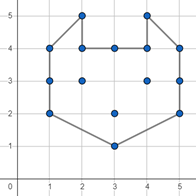
\includegraphics[width=0.7\textwidth]{pic/721.png} }
\end{minipage}
\end{figure}



---------------

Автор -- Алёна Холмогорова, М3209\question
Приведите  пример  нескольких бинарных отношений:
\begin{enumerate}
	\renewcommand{\labelenumi}{\alph{enumi})}
	\item отношение, которое является композиции нескольких бинарных отношений,  которое  обладает любым типом соответсвия  и симметрично (укажите все бинарные отношения, участвующие в композиции)
	\item два отношения, первое -- частично упорядочивает множество, на котором оно задано и второе -- полностью упорядочивает (обязательно покажите порядок элементов множества, полученный упордочиванием бинарным отношением)
	\item отношение, такое что обратное к нему  обладает одинаковыми с ним свойствами и оба функциональны (докажите, что свойства сохранаются)
\end{enumerate}

\underline{примечание:} важно показать  множества, на которых задано бинарное отношение и доказать, что ваше бинарное отношение обладает заданными свойствами
\question
Петя решил поучаствовать в конкурсе рисунков, к сожалению, проблема была в том, что он совершенно не умел рисовать, но Петя был умным мальчиком, который знал бинарные отношения.
\\На декартовом произведении множества $A = \{-2, -1, 0, 1, 2, 3, 4, 5, 6, 7, 8, 9, 10, 11\}$ заданы бинарные отношения:
\begin{equation*}
R_1 = {(0, -2), (2, 0), (6, -2), (8, 0), (9, -2), (12, -2), (11, -1), (11, 1), (12, 2), (9, 2), (8, 0), (6, 2), (5, 5), (0, 5), (6, 7), (0, 6)}
\end{equation*}
\begin{center}и\end{center}
\begin{equation*}
R_2 = \{(10, -1), (10, -1), (9, 0)\}
\end{equation*}
Помогите Пете выиграть в конкурсе! Постройте композиции отношений $R_1^{-1}, R_2^{-1}$ и изобразите полученный результат на декартовой системе координат (задание можно дополнять другими композициями).
\\
---------------

Автор -- Анастасия Стеценко, М3207\question
Даны отношения $R_1$, $R_2$ и $R_3$ на множестве $A = \{1; 2; 3; 4; 5;\}$ 
\begin{enumerate}
	\renewcommand{\labelenumi}{\alph{enumi})}
	\item $R_1 = \{(1; 1); (2; 2); (3; 3); (2; 1);\}$
	\item $R_2 = \{(1; 2); (3; 4); (3; 5); (4; 5)\}$
	\item $R_2 = \{(1; 3); (1; 5); (3; 4); (4; 5)\}$
\end{enumerate}

\begin{enumerate}
	\renewcommand{\labelenumi}{\alph{enumi})}
	\item $(R_1 \cap R_2) \cup R_3$
	\item $R_1 \cup R_3$
	\item $R_1^3 \cap R_3^{-1}$
	\item $R_3 \cup R_2^2$
	\item $R_2 \cup \overline{R_1}$
\end{enumerate}

определите основные свойства, получившихся отношений
определите какие свойства сохраняются относительно исходных отношений $R_1$, $R_2$ и $R_3$

\underline{примечание:} результатом может быть пустое множество

\end{questions}
\newpage
%%% begin test
\begin{flushright}
\begin{tabular}{p{2.8in} r l}
%\textbf{\class} & \textbf{ФИО:} & \makebox[2.5in]{\hrulefill}\\
\textbf{\class} & \textbf{ФИО:} &Радченко Андрей Александрович
\\

\textbf{\examdate} &&\\
%\textbf{Time Limit: \timelimit} & Teaching Assistant & \makebox[2in]{\hrulefill}
\end{tabular}\\
\end{flushright}
\rule[1ex]{\textwidth}{.1pt}


\begin{questions}
\question
Вы -- великая искательница сокровищ Лариса Крафтовое. Очередное путешествие забросило вас в подземные гробницы Сигизмунда I. К сожалению, на вашем пути встал очень назойливый мраморный привратник, который по всем канонам жанра имеет для вас пару загадок.
\\
\\
Привратник загадывает свое множество $X$, а также дает вам парочку других $(A,B,C…)$, объединяя, пересекая, дополняя и/или выполняя разность над которыми вы должны получить его множество. Загвоздка лишь в том, что привратник сам выбирает расстановку множеств в формуле, поэтому вам остается лишь вставить операции и расставить скобки (при надобности).

\paragraph{Загадка 1:}
\begin{equation*}
    X=\{1,2,5,6\}
\end{equation*}
\begin{equation*}
    A=\{1,2,3,4\}; B=\{2,3,4,5\}; C=\{2,5\}; D=\{4,5,6\}
    \end{equation*}
\begin{equation*}
    A ? B ? C ? D = X
\end{equation*}

\paragraph{Загадка 2:}
\begin{equation*}
    X=\{3,4,5\}
\end{equation*}
\begin{equation*}
    A=\{2,3,4,5\}; B=\{1,2,3\}; C=\{3,4,5\}; D=\{1,5,6\}
    \end{equation*}
\begin{equation*}
    A ? B ? C ? D = X
\end{equation*}

---------------

Автор -- Константин Васильев, М3213\question
Упростите следующее выражение с учетом того, что $A\subset B \subset C \subset D \subset U; A \neq \emptyset$
\begin{equation*}
	\overline{A} \cap \overline{C} \cap D \cup \overline{B} \cap \overline{C} \cap D \cup A \cap B
\end{equation*}

Примечание: $U$ -- универсум\question
Укажите номера множеств, являющихся подмножествами множества
\begin{equation*}
	Q = \bar{A} \cup B \cap C \cup \bar{C} \cap \bar{D}
\end{equation*}

\begin{enumerate}
	\renewcommand{\labelenumi}{\arabic{enumi})}
	\item $P = B \cap C \cap D \cup \bar{A} \cap B \cap C$;
	\item $P = \bar{B} \cap \bar{C} \cap D \cup B \cap \bar{C} \cap \bar{D}$;
	\item $P = A \cap \bar{B} \cap D \cup A \cap C \cap D$;
	\item $P = \bar{B} \cap \bar{C} \cup \bar{A} \cap \bar{B} \cap D$.
\end{enumerate}
\question
Постройте разбиения множеств:
\begin{enumerate}
	\renewcommand{\labelenumi}{\alph{enumi})}
	\item $A = \{6, 7, 8, 9, 11, 14, 34, 91, 55, 65, 76, 28, 93, 94, \};$
	\item $B = \{8, 9, 11, 22, 33, 44, 55, 65, 67, 87, 91, 92, 93, 94, 95, 98\}$
	\item $A \cup B$
	\item $A \cap B$
\end{enumerate}
Таким образом, чтобы все разбиения имели как минимум 2 одинаковых множества в разбиениях.
Мощность каждого разбиение была более 4.
Докажите, что ваш ответ соответствует указанным условиям!\question
Упростить выражения, используя свойства операций над множествами:

\begin{enumerate}
	\renewcommand{\labelenumi}{\alph{enumi})}
	\item $(A\cap B \cap C \cap D) \cup (\overline{\overline{A}\cup C}\cap D) \cup (D\cap\overline{(\overline{A}+C)+D})\cup (\overline{A}\cap B\cap C \cap D)$;
	\item $(A\cap B \cap C \cap D \cap (A\cup D \cup \overline{A\cap D}))\cup \overline{\overline{A}\cup \overline{D}\cup C\cup D}\cup (A\cap B \cap (D\cap\overline{C}\cup C\cap\overline{D}))$.
\end{enumerate}
\question
Дано отношение на множестве $\{1, 2, 3, 4, 5\}$ 
\begin{equation*}
	aRb \iff b > a
\end{equation*}

(ЧАСТЬ 1) Какими основным свойствами обладает отношение? (Дайте обоснованный ответ по всем пунктам ниже: докажите наличие или отсутствие свойств)  
\begin{enumerate}
	\renewcommand{\labelenumi}{\alph{enumi})}
	\item рефлексивность / антирефлексивность / нерефлексивность
	\item симметричность / антисимметричность / асимметричность / несимметричность
	\item транзитивность / антитранзитивность / нетранзитивность
\end{enumerate}

(ЧАСТЬ 2) Обоснуйте свой ответ по каждому из приведенных ниже вопросов:
\begin{enumerate}
	\renewcommand{\labelenumi}{\alph{enumi})}
    \item Является ли это отношение отношением эквивалентности?
    \item Является ли это отношение функциональным?
    \item Каким из отношений соответствия (одно-многозначным, много-многозначный и т.д.) оно является?
    \item К каким из отношений порядка (строгого, не строгого и т.д.) можно отнести данное отношение?
\end{enumerate}
\question
Установите, является ли каждое из перечисленных ниже отношений на А ($R \subseteq A \times A$) отношением эквивалентности (обоснование ответа обязательно). Для каждого отношения эквивалентности постройте классы 
эквивалентности и постройте граф отношения:
\begin{enumerate}
	\renewcommand{\labelenumi}{\alph{enumi})}
	\item $A = \{a, b, c, d, p, t\}$ задано отношение $R = \{(a, a), (b, b), (b, c), (b, d), (c, b), (c, c), (c, d), (d, b), (d, c), (d, d), (p,p), (t,t)\}$
	\item $A = \{-10, -9, ..., 9, 10\}$ и отношение $R = \{(a,b)|a^{3} = b^{3}\}$
	\item $F(x)=x^{2}+1$, где $x \in A = [-2, 4]$ и отношение $R = \{(a,b)|F(a) = F(b)\}$
\end{enumerate}\question
Приведите  пример  нескольких бинарных отношений:
\begin{enumerate}
	\renewcommand{\labelenumi}{\alph{enumi})}
	\item отношение, которое является композиции нескольких бинарных отношений,  которое  нестрого порядка и функционально (укажите все бинарные отношения, участвующие в композиции)
	\item отношение, которое частично упорядочивает множество и как минимум 6 элементов упорядочены (обязательно покажите порядок элементов множества, полученный упордочиванием бинарным отношением)
	\item отношение, такое что обратное к нему  обладает одинаковыми с ним свойствами и оба эквивалентны (докажите, что свойства сохранаются)
\end{enumerate}

\underline{примечание:} важно показать  множества, на которых задано бинарное отношение и доказать, что ваше бинарное отношение обладает заданными свойствами
\question
Довольные студенты ИТМО сдали летнюю сессию и намерены поехать домой на некоторое время. К сожалению, чтобы добраться до пункта назначения, им потребуется сделать несколько пересадок.

Пусть множество всех населенных пунктов выглядит как: $A = \{1, 2, 3, 4, 5, 6\}$.
\\
Тогда $R = \{(1, 3), (3, 1), (2, 4), (4, 2), (1, 5), (5, 1), (2, 3), (3, 2)\}$ -- можно доехать на автобусе, $S = \{(5, 6), (6, 5), (3, 6), (6, 3)\}$ -- можно долететь на самолете.

\begin{itemize}
    \item Найдите такие пары пунктов, для перемещения между которыми надо проехать на автобусе, а затем воспользоваться самолетом и наоборот.
    \item Найдите пары пунктов, между которыми можно перемещаться на автобусе с одной пересадкой (пары вида (1, 1) не стоит указывать в ответе).
    \item Найдите пары пунктов, между которыми можно перемещаться на самолете с одной пересадкой в промежуточном пункте.
\end{itemize}
\\
---------------

Автор -- Елизавета Котельникова, М3212\question
Даны отношения $R_1$, $R_2$ и $R_3$ на множестве $A = \{1; 2; 3; 4; 5;\}$ 
\begin{enumerate}
	\renewcommand{\labelenumi}{\alph{enumi})}
	\item $R_1 = \{(1; 1); (2; 2); (3; 3); (2; 1); (1; 2); \}$
	\item $R_2 = \{(1; 1); (2; 2); (1; 3); (3; 4); (3; 5);\}$
	\item $R_2 = \{(1; 1); (2; 2);  (1; 5); (3; 4); (3; 5); (4; 5)\}$
\end{enumerate}

\begin{enumerate}
	\renewcommand{\labelenumi}{\alph{enumi})}
	\item $R_1 \cap R_2$
	\item $R_1 \cup R_2 \cup R_3$
	\item $R_1^2 \cap R_3^{-1}$
	\item $R_1 \cup R_3^4$
	\item $R_1 \cup \overline{R_3}$
\end{enumerate}

определите основные свойства, получившихся отношений
определите какие свойства сохраняются относительно исходных отношений $R_1$, $R_2$ и $R_3$ 

\underline{примечание:} результатом может быть пустое множество

\end{questions}
\newpage
%%% begin test
\begin{flushright}
\begin{tabular}{p{2.8in} r l}
%\textbf{\class} & \textbf{ФИО:} & \makebox[2.5in]{\hrulefill}\\
\textbf{\class} & \textbf{ФИО:} &Рифад Мд Абу Хуссаин
\\

\textbf{\examdate} &&\\
%\textbf{Time Limit: \timelimit} & Teaching Assistant & \makebox[2in]{\hrulefill}
\end{tabular}\\
\end{flushright}
\rule[1ex]{\textwidth}{.1pt}


\begin{questions}
\question
В самом мирном городе мира, Лос-Сантосе, орудуют несколько бандитских группировок: Гроув-стрит, Баллос и Вагос. Некоторые районы города, для удобства бандитов помеченные цифрами \{0...9\}, находятся под влиянием этих банд:
\begin{itemize}
    \item Гроув-стрит: \{1, 2, 3, 7, 9\}
    \item Баллос: \{1, 3, 7, 8\}
    \item Вагос: \{4, 6, 7, 9\}
\end{itemize}
Районы, оказавшиеся под влиянием нескольких банд, называются спорными территориями.
\\
\\
В один прекрасный летний день Си-Джей увидел на стене своего дома граффити с сообщением от информатора из банды Баллосов. Для конспирации он оставил его в таком виде:
\begin{equation*}
B \cap \overline{G} \cup G \cap V \cap \overline{B} \cup G \cap B \cap \overline{V}
\end{equation*}
В нем содержатся номера районов, на которые полиция планирует совершить облаву. Вам, как самому умному представителю Гроув-Стрит, необходимо расшифровать граффити, а затем ответить на следующие вопросы:

\begin{itemize}
    \item Какие районы не под контролем ни одной из этих банд?
    \item Какое количество районов охватывают все три банды?
    \item На какие из районов, находящихся под вашим влиянием, будет совершена облава?
\end{itemize}

---------------

Автор -- Константин Васильев, М3213\question
Упростите следующее выражение с учетом того, что $A\subset B \subset C \subset D \subset U; A \neq \emptyset$
\begin{equation*}
	A \cap B  \cap \overline{C} \cup \overline{C} \cap D \cup B \cap C \cap D
\end{equation*}

Примечание: $U$ -- универсум\question
Укажите номера множеств, являющихся подмножествами множества
\begin{equation*}
	Q = \bar{A} \cap C \cup A \cap \bar{B} \cup A \cap \bar{C} \cup \bar{A} \cap B \cap D
\end{equation*}

\begin{enumerate}
	\renewcommand{\labelenumi}{\arabic{enumi})}
	\item $P = A \cap \bar{B} \cap D \cup \bar{A} \cap \bar{B} \cap C$;
	\item $P = A \cap B \cap D \cup \bar{A} \cap \bar{C} \cap D$;
	\item $P = B \cap \bar{C} \cap \bar{D} \cup A \cap B \cap \bar{C}$;
	\item $P = A \cap \bar{C} \cap \bar{D} \cup \bar{A} \cap \bar{B} \cap D$.
\end{enumerate}
\question
Постройте разбиения множеств:
\begin{enumerate}
	\renewcommand{\labelenumi}{\alph{enumi})}
	\item $A = \{6, 7, 8, 9, 11, 14, 34, 91, 55, 65, 76, 28, 19, 93, 94, \};$
	\item $B = \{0, 1, 2, 3, 4, 5, 6, 7, 8, 9, 11, 22, 33, 44, 55, 65, 111, 113, 67, 87, 91, 92, 93, 94, 95, 98\}$
	\item $A \cup B$
	\item $A \cap B$
\end{enumerate}
Таким образом, чтобы все разбиения имели как минимум 2 одинаковых множества в разбиениях.
Мощность каждого разбиение была более 4.
Докажите, что ваш ответ соответствует указанным условиям!\question
Пусть у нас есть $P$ -- множество студентов города Санкт-Петербург, из них $A$ -- третьекурсники, $B$ -- проходят профессиональную переподготовку, а $C$ -- стажируются в Яндексе. Для статьи “Как учиться на третьем курсе университета ИТМО, проходить профессиональную подготовку и не умереть” Мегабайт создал выборку $D$.
\\
\\
Упростите множество $E = (P \cap D \cup C \cap \overline{B} \cap \overline{D} \cup B \cap A \cap \overline{C}) \cap \overline{C} \cap \overline{D} \cap P$, а затем опишите его словами.
\\
\\
---------------

Автор -- Антонина Чернова, М33081\question
Бабушка Люда потеряла книгу со своими лучшими рецептами напитков. Вы, как добросовестный внук, проводивший у любимой бабушки большое количество времени, помните из чего бабуля варила вкуснейшие морсы и компоты. Обычно бабушка варила напитки из двух видов ягод и фруктов среди которых были: Малина, Облепиха, Жимолость, Смородина, Яблоки, Абрикосы и Груши. Также вы помните, что нельзя совмещать между собой Облепиху и красные ягоды, Абрикос и ягоды, Яблоко и ягоды. Постройте бинарное отношение содержащее все возможные сочетания для напитков таким образом, чтобы ингредиенты не повторялись.
\\
Ответьте на вопросы касаемо построенного бинарного отношения:
\begin{itemize}
    \item Какими свойствами обладает данное БО? Обоснуйте
    \item Является ли данное отношение функциональным?
    \item Каким из отношений соответствия оно является? (одно-многозначным, много-многозначным и т.д.)
\end{itemize}
\\
---------------

Автор -- Максим Акимцов, М3208\question
Одним теплым вечером кот Степан вдохновился картинами, которые он увидел в Эрмитаже, и решил нарисовать свой автопортрет. Так как у Степана была тетрадка в клетку, оставшаяся после пройденного курса дискретной математики, он решил рисовать там. Нарисовав автопортрет ровно по клеткам, он подумал, что можно дорисовать координатные оси и обозначить все целые точки, пересекающиеся с контуром портрета. На обратной стороне листка он увидел конспект лекции по бинарным отношениям. Но так как память у кота не очень хорошая, он решил попросить вас найти бинарное отношение, соответствующее рисунку и два таких бинарных отношения, чтобы в композиции они давали исходное бинарное отношение и изобразить их.
\\
\begin{figure}[h]

\begin{minipage}[h]{0.55\linewidth}
\end{minipage}
\begin{minipage}[h]{0.45\linewidth}
\center{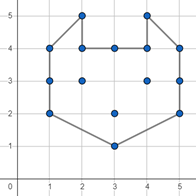
\includegraphics[width=0.7\textwidth]{pic/721.png} }
\end{minipage}
\end{figure}



---------------

Автор -- Алёна Холмогорова, М3209\question
Докажите (с подробным объяснением) или опровергните (приведя контрпример) следующие утверждения о бинарных отношениях $R \subseteq M^2$ и $S \subseteq M^2$:
\begin{itemize}
    \item Если $R$ и $S$ рефлексивны, то $R \circ S$ тоже рефлексивно.
    \item Если $R$ и $S$ симметрично, то $R \circ S$ тоже симметрично.
    \item Если $R$ и $S$ транзитивно, то $R \circ S$ тоже транзитивно.
    \item Если $R$ и $S$ рефлексивны, то $R \circ S$ тоже рефлексивно.
    \item Если $R$ и $S$ симметрично, то $R \circ S$ тоже симметрично.
    \item Если $R$ и $S$ транзитивно, то $R \circ S$ тоже транзитивно.
\end{itemize}
\\
---------------

Автор -- Алексей Лёвушкин, М3204\question
В перерыве между парами дискретной математики вы с друзьями решили зарубиться в домино. Иллюстрация ниже визуализирует данный момент игры.

\\
\begin{figure}[h]

\begin{minipage}[h]{0.55\linewidth}
\end{minipage}
\begin{minipage}[h]{0.45\linewidth}
\center{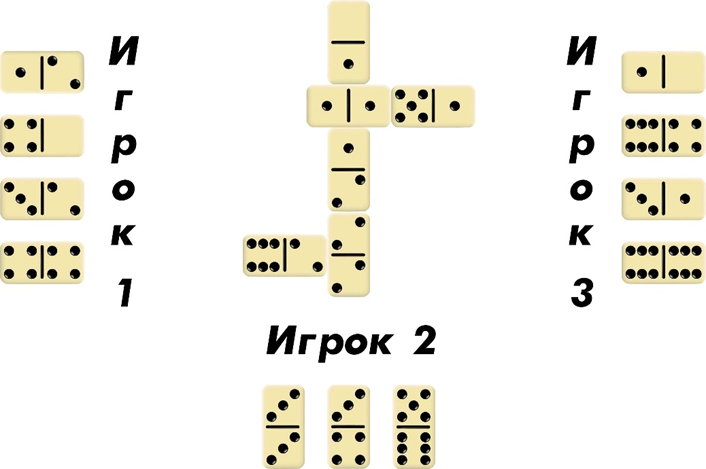
\includegraphics[width=0.7\textwidth]{pic/941.png} }
\end{minipage}
\end{figure}

Так как вы — умные студенты, вам стало интересно интерпретировать партию в виде бинарных отношений. Запишите отношения:
\begin{itemize}
    \item $G = \{(a,b)|a$ и $b$ – стороны свободных доминошек, лежащих на столе, где a – свободная сторона$\}$
    \item $R_1 = \{(a,b)|a$ и $b$ – стороны одной доминошки в руке у первого игрока$\}$
    \item $R_2 = \{(a,b)|a$ и $b$ – стороны одной доминошки в руке у второго игрока$\}$
    \item $R_3 = \{(a,b)|a$ и $b$ – стороны одной доминошки в руке у третьего игрока$\}$
\end{itemize}

Используя операцию композиции, составьте новые бинарные отношения:
\begin{itemize}
    \item $P_1$ – возможные ходы у первого игрока
    \item $P_2$ – возможные ходы у второго игрока
    \item $P_3$ – возможные ходы у третьего игрока
\end{itemize}


Ходом является пара крайних номеров стоящих рядом доминошек.
\\
---------------

Автор -- Константин Васильев, М3213\question
Даны отношения $R_1$, $R_2$ и $R_3$ на множестве $A = \{1; 2; 3; 4; 5;\}$ 
\begin{enumerate}
	\renewcommand{\labelenumi}{\alph{enumi})}
	\item $R_1 = \{(3; 2); (3; 1); (1; 3)\}$
	\item $R_2 = \{(1; 2); (2; 2); (1; 3); (1; 5); (2; 3); (4; 5)\}$
	\item $R_2 = \{(1; 2); (2; 2); (3; 4); (3; 5); (4; 5)\}$
\end{enumerate}

\begin{enumerate}
	\renewcommand{\labelenumi}{\alph{enumi})}
	\item $R_1 \cap R_2$
	\item $(R_1 \cup R_2) \cap R_3$
	\item $R_3^2 \cap R_3^{-1}$
	\item $R_3 \cup \overline{R_2^2}$
	\item $R_1 \cup \overline{R_2} \cup R_3$
\end{enumerate}

определите основные свойства, получившихся отношений
определите какие свойства сохраняются относительно исходных отношений $R_1$, $R_2$ и $R_3$ 

\underline{примечание:} результатом может быть пустое множество

\end{questions}
\newpage
%%% begin test
\begin{flushright}
\begin{tabular}{p{2.8in} r l}
%\textbf{\class} & \textbf{ФИО:} & \makebox[2.5in]{\hrulefill}\\
\textbf{\class} & \textbf{ФИО:} &Руденко Александр Александрович
\\

\textbf{\examdate} &&\\
%\textbf{Time Limit: \timelimit} & Teaching Assistant & \makebox[2in]{\hrulefill}
\end{tabular}\\
\end{flushright}
\rule[1ex]{\textwidth}{.1pt}


\begin{questions}
\question
Вы -- великая искательница сокровищ Лариса Крафтовое. Очередное путешествие забросило вас в подземные гробницы Сигизмунда I. К сожалению, на вашем пути встал очень назойливый мраморный привратник, который по всем канонам жанра имеет для вас пару загадок.
\\
\\
Привратник загадывает свое множество $X$, а также дает вам парочку других $(A,B,C…)$, объединяя, пересекая, дополняя и/или выполняя разность над которыми вы должны получить его множество. Загвоздка лишь в том, что привратник сам выбирает расстановку множеств в формуле, поэтому вам остается лишь вставить операции и расставить скобки (при надобности).

\paragraph{Загадка 1:}
\begin{equation*}
    X=\{1,2,5,6\}
\end{equation*}
\begin{equation*}
    A=\{1,2,3,4\}; B=\{2,3,4,5\}; C=\{2,5\}; D=\{4,5,6\}
    \end{equation*}
\begin{equation*}
    A ? B ? C ? D = X
\end{equation*}

\paragraph{Загадка 2:}
\begin{equation*}
    X=\{3,4,5\}
\end{equation*}
\begin{equation*}
    A=\{2,3,4,5\}; B=\{1,2,3\}; C=\{3,4,5\}; D=\{1,5,6\}
    \end{equation*}
\begin{equation*}
    A ? B ? C ? D = X
\end{equation*}

---------------

Автор -- Константин Васильев, М3213\question
Упростите следующее выражение с учетом того, что $A\subset B \subset C \subset D \subset U; A \neq \emptyset$
\begin{equation*}
	\overline{B} \cap \overline{C} \cap D \cup \overline{A} \cap \overline{C} \cap D \cup \overline{A} \cap B
\end{equation*}

Примечание: $U$ -- универсум\question
Укажите номера множеств, являющихся подмножествами множества
\begin{equation*}
	Q = \bar{A} \cap B \cup A \cap \bar{B} \cup A \cap \bar{C} \cup \bar{A} \cap C \cap \bar{D}
\end{equation*}

\begin{enumerate}
	\renewcommand{\labelenumi}{\arabic{enumi})}
	\item $P = A \cap \bar{B} \cap D \cup \bar{A} \cap \bar{B} \cap C$;
	\item $P = A \cap B \cap D \cup \bar{A} \cap \bar{C} \cap D$;
	\item $P = B \cap \bar{C} \cap \bar{D} \cup A \cap B \cap \bar{C}$;
	\item $P = A \cap \bar{C} \cap \bar{D} \cup \bar{A} \cap \bar{B} \cap D$.
\end{enumerate}
\question
Постройте разбиения множеств:
\begin{enumerate}
	\renewcommand{\labelenumi}{\alph{enumi})}
	\item $A = \{6, 7, 8, 9, 11, 14, 34, 54, 47, 18, 91\};$
	\item $B = \{0, 1, 2, 3, 4, 5, 6, 7, 8, 9\}$
	\item $A \cap B$
\end{enumerate}
Таким образом, чтобы все разбиения имели как минимум 2 одинаковых множества в разбиениях.
Мощность каждого разбиение была более 3.
Докажите, что ваш ответ соответствует указанным условиям!\question
Упростить выражения, используя свойства операций над множествами:

\begin{enumerate}
	\renewcommand{\labelenumi}{\alph{enumi})}
	\item $(A \cap B \cap C \cap \bar{D}) \cup(\bar{A} \cap C) \cup(\bar{B} \cap C) \cup(C \cap D)$;
	\item $(\bar{A} \cup B \cup \bar{C}) \cap(A \cap \bar{B} \cap C) \cap \overline{(A \cup C)}$.
\end{enumerate}
\question
Дано отношение на множестве $\{1, 2, 3, 4, 5\}$ 
\begin{equation*}
	aRb \iff a \leqslant b
\end{equation*}

(ЧАСТЬ 1) Какими основным свойствами обладает отношение? (Дайте обоснованный ответ по всем пунктам ниже: докажите наличие или отсутствие свойств)  
\begin{enumerate}
	\renewcommand{\labelenumi}{\alph{enumi})}
	\item рефлексивность / антирефлексивность / нерефлексивность
	\item симметричность / антисимметричность / асимметричность / несимметричность
	\item транзитивность / антитранзитивность / нетранзитивность
\end{enumerate}

(ЧАСТЬ 2) Обоснуйте свой ответ по каждому из приведенных ниже вопросов:
\begin{enumerate}
	\renewcommand{\labelenumi}{\alph{enumi})}
    \item Является ли это отношение отношением эквивалентности?
    \item Является ли это отношение функциональным?
    \item Каким из отношений соответствия (одно-многозначным, много-многозначный и т.д.) оно является?
    \item К каким из отношений порядка (строгого, не строгого и т.д.) можно отнести данное отношение?
\end{enumerate}
\question
Одним теплым вечером кот Степан вдохновился картинами, которые он увидел в Эрмитаже, и решил нарисовать свой автопортрет. Так как у Степана была тетрадка в клетку, оставшаяся после пройденного курса дискретной математики, он решил рисовать там. Нарисовав автопортрет ровно по клеткам, он подумал, что можно дорисовать координатные оси и обозначить все целые точки, пересекающиеся с контуром портрета. На обратной стороне листка он увидел конспект лекции по бинарным отношениям. Но так как память у кота не очень хорошая, он решил попросить вас найти бинарное отношение, соответствующее рисунку и два таких бинарных отношения, чтобы в композиции они давали исходное бинарное отношение и изобразить их.
\\
\begin{figure}[h]

\begin{minipage}[h]{0.55\linewidth}
\end{minipage}
\begin{minipage}[h]{0.45\linewidth}
\center{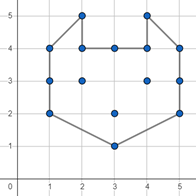
\includegraphics[width=0.7\textwidth]{pic/721.png} }
\end{minipage}
\end{figure}



---------------

Автор -- Алёна Холмогорова, М3209\question
Докажите (с подробным объяснением) или опровергните (приведя контрпример) следующие утверждения о бинарных отношениях $R \subseteq M^2$ и $S \subseteq M^2$:
\begin{itemize}
    \item Если $R$ и $S$ рефлексивны, то $R \circ S$ тоже рефлексивно.
    \item Если $R$ и $S$ симметрично, то $R \circ S$ тоже симметрично.
    \item Если $R$ и $S$ транзитивно, то $R \circ S$ тоже транзитивно.
    \item Если $R$ и $S$ рефлексивны, то $R \circ S$ тоже рефлексивно.
    \item Если $R$ и $S$ симметрично, то $R \circ S$ тоже симметрично.
    \item Если $R$ и $S$ транзитивно, то $R \circ S$ тоже транзитивно.
\end{itemize}
\\
---------------

Автор -- Алексей Лёвушкин, М3204\question
Вася хочет устроиться бэкенд разработчиком в ИТМО, работать с ИСУ. На собеседовании тимлид дал ему тестовое задание, чтобы определить его уровень знаний:
\\
\begin{figure}[h]

\begin{minipage}[h]{0.55\linewidth}
\end{minipage}
\begin{minipage}[h]{0.45\linewidth}
\center{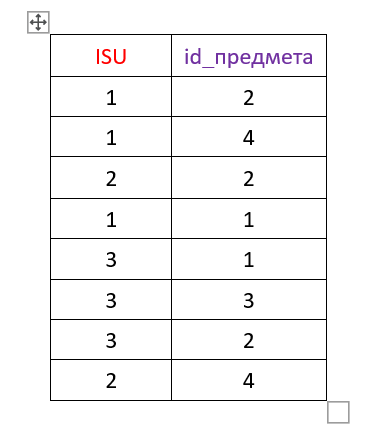
\includegraphics[width=0.7\textwidth]{pic/911.png}\includegraphics[width=0.7\textwidth]{pic/912.png} }
\end{minipage}
\end{figure}

В базе данных расписания ИТМО есть 2 таблицы:
\begin{itemize}
    \item В таблице 1 (рис. 1) каждому студенту по его номеру ИСУ сопоставлены предметы по их id. У одного номера ИСУ (студента) может быть много предметов, при этом на один предмет может ходить несколько студентов.
    \item В таблице 2 (рис. 2) каждому дню недели по его id (порядковый номер: 1-пн, 2-вт, 3-ср и т. д.) сопоставлены предметы по их id. В один день могут проводиться пары по нескольким предметам, при этом пары по одному предмету могут проходить несколько дней в неделе.
\end{itemize}
От Васи требуется по имеющимся данным вывести все возможные кортежи вида:

\begin{center}(номер ИСУ, день когда у этого студента есть пары)\end{center}

Например, ответ вида $\{(1, 1), (1, 5), (2, 1)\}$ будет означать что студент с ISU №1 имеет пары в понедельник и пятницу, а студент с ISU №2 имеет пары только в понедельник.

Помогите Васе решить данную задачу, используя ваши знания по дискретной математике.

---------------

Автор -- Тимур Гонтарь, М3206\question
Даны отношения $R_1$, $R_2$ и $R_3$ на множестве $A = \{1; 2; 3; 4; 5;\}$ 
\begin{enumerate}
	\renewcommand{\labelenumi}{\alph{enumi})}
	\item $R_1 = \{(3; 2); (3; 1); (1; 3)\}$
	\item $R_2 = \{(1; 2); (2; 2); (1; 3); (4; 5)\}$
	\item $R_3 = \{(1; 2); (2; 2); (3; 4); (3; 5); (4; 5)\}$
\end{enumerate}

\begin{enumerate}
	\renewcommand{\labelenumi}{\alph{enumi})}
	\item $R_1 \cap R_2^{-1} \cup R_3^2$
	\item $(R_1 \cup R_2) \cap R_3$
	\item $R_3^2 \cap R_3^{-1}$
	\item $R_3^{-1} \cup \overline{R_2^{-1}}$
	\item $R_1^{-1} \cup \overline{R_2} \cup R_3$
\end{enumerate}

определите основные свойства, получившихся отношений
определите какие свойства сохраняются относительно исходных отношений $R_1$, $R_2$ и $R_3$ 

\underline{примечание:} результатом может быть пустое множество

\end{questions}
\newpage
%%% begin test
\begin{flushright}
\begin{tabular}{p{2.8in} r l}
%\textbf{\class} & \textbf{ФИО:} & \makebox[2.5in]{\hrulefill}\\
\textbf{\class} & \textbf{ФИО:} &Тулай Максим Витальевич
\\

\textbf{\examdate} &&\\
%\textbf{Time Limit: \timelimit} & Teaching Assistant & \makebox[2in]{\hrulefill}
\end{tabular}\\
\end{flushright}
\rule[1ex]{\textwidth}{.1pt}


\begin{questions}
\question
В самом мирном городе мира, Лос-Сантосе, орудуют несколько бандитских группировок: Гроув-стрит, Баллос и Вагос. Некоторые районы города, для удобства бандитов помеченные цифрами \{0...9\}, находятся под влиянием этих банд:
\begin{itemize}
    \item Гроув-стрит: \{1, 2, 3, 7, 9\}
    \item Баллос: \{1, 3, 7, 8\}
    \item Вагос: \{4, 6, 7, 9\}
\end{itemize}
Районы, оказавшиеся под влиянием нескольких банд, называются спорными территориями.
\\
\\
В один прекрасный летний день Си-Джей увидел на стене своего дома граффити с сообщением от информатора из банды Баллосов. Для конспирации он оставил его в таком виде:
\begin{equation*}
B \cap \overline{G} \cup G \cap V \cap \overline{B} \cup G \cap B \cap \overline{V}
\end{equation*}
В нем содержатся номера районов, на которые полиция планирует совершить облаву. Вам, как самому умному представителю Гроув-Стрит, необходимо расшифровать граффити, а затем ответить на следующие вопросы:

\begin{itemize}
    \item Какие районы не под контролем ни одной из этих банд?
    \item Какое количество районов охватывают все три банды?
    \item На какие из районов, находящихся под вашим влиянием, будет совершена облава?
\end{itemize}

---------------

Автор -- Константин Васильев, М3213\question
Упростите следующее выражение с учетом того, что $A\subset B \subset C \subset D \subset U; A \neq \emptyset$
\begin{equation*}
	A \cap C  \cap D \cup B \cap \overline{C} \cap D \cup B \cap C \cap D
\end{equation*}

Примечание: $U$ -- универсум\question
Укажите номера множеств, являющихся подмножествами множества
\begin{equation*}
	Q = A \cap \bar{D} \cup B \cap C \cup \bar{A} \cap \bar{B} \cap D \cup A \cap C
\end{equation*}

\begin{enumerate}
	\renewcommand{\labelenumi}{\arabic{enumi})}
	\item $P = B \cap C \cap D \cup \bar{A} \cap B \cap C$;
	\item $P = \bar{B} \cap \bar{C} \cap D \cup B \cap \bar{C} \cap \bar{D}$;
	\item $P = A \cap \bar{B} \cap D \cup A \cap C \cap D$;
	\item $P = \bar{B} \cap \bar{C} \cup \bar{A} \cap \bar{B} \cap D$.
\end{enumerate}
\question
Постройте разбиения множеств:
\begin{enumerate}
	\renewcommand{\labelenumi}{\alph{enumi})}
	\item $A = \{6, 7, 8, 9, 11, 14, 34, 54, 47, 18, 91\};$
	\item $B = \{0, 1, 2, 3, 4, 5, 6, 7, 8, 9\}$
	\item $A \cap B$
\end{enumerate}
Таким образом, чтобы все разбиения имели как минимум 2 одинаковых множества в разбиениях.
Мощность каждого разбиение была более 3.
Докажите, что ваш ответ соответствует указанным условиям!\question
Упростить выражения, используя свойства операций над множествами:

\begin{enumerate}
	\renewcommand{\labelenumi}{\alph{enumi})}
	\item $(A\cap B \cap C \cap D) \cup (\overline{\overline{A}\cup C}\cap D) \cup (D\cap\overline{(\overline{A}+C)+D})\cup (\overline{A}\cap B\cap C \cap D)$;
	\item $(A\cap B \cap C \cap D \cap (A\cup D \cup \overline{A\cap D}))\cup \overline{\overline{A}\cup \overline{D}\cup C\cup D}\cup (A\cap B \cap (D\cap\overline{C}\cup C\cap\overline{D}))$.
\end{enumerate}
\question
Дано отношение на множестве $\{1, 2, 3, 4, 5\}$ 
\begin{equation*}
	aRb \iff a \leqslant b
\end{equation*}

(ЧАСТЬ 1) Какими основным свойствами обладает отношение? (Дайте обоснованный ответ по всем пунктам ниже: докажите наличие или отсутствие свойств)  
\begin{enumerate}
	\renewcommand{\labelenumi}{\alph{enumi})}
	\item рефлексивность / антирефлексивность / нерефлексивность
	\item симметричность / антисимметричность / асимметричность / несимметричность
	\item транзитивность / антитранзитивность / нетранзитивность
\end{enumerate}

(ЧАСТЬ 2) Обоснуйте свой ответ по каждому из приведенных ниже вопросов:
\begin{enumerate}
	\renewcommand{\labelenumi}{\alph{enumi})}
    \item Является ли это отношение отношением эквивалентности?
    \item Является ли это отношение функциональным?
    \item Каким из отношений соответствия (одно-многозначным, много-многозначный и т.д.) оно является?
    \item К каким из отношений порядка (строгого, не строгого и т.д.) можно отнести данное отношение?
\end{enumerate}
\question
Одним теплым вечером кот Степан вдохновился картинами, которые он увидел в Эрмитаже, и решил нарисовать свой автопортрет. Так как у Степана была тетрадка в клетку, оставшаяся после пройденного курса дискретной математики, он решил рисовать там. Нарисовав автопортрет ровно по клеткам, он подумал, что можно дорисовать координатные оси и обозначить все целые точки, пересекающиеся с контуром портрета. На обратной стороне листка он увидел конспект лекции по бинарным отношениям. Но так как память у кота не очень хорошая, он решил попросить вас найти бинарное отношение, соответствующее рисунку и два таких бинарных отношения, чтобы в композиции они давали исходное бинарное отношение и изобразить их.
\\
\begin{figure}[h]

\begin{minipage}[h]{0.55\linewidth}
\end{minipage}
\begin{minipage}[h]{0.45\linewidth}
\center{\includegraphics[width=0.7\textwidth]{pic/721.png} }
\end{minipage}
\end{figure}



---------------

Автор -- Алёна Холмогорова, М3209\question
Пусть имеется бинарное отношение $R$ на $ A \times A$. Докажите, что если $R$ -- одновременно и отношение эквивалентности и отношение частичного порядка, то оно -- отношение равенства.
\\
---------------

Автор -- Алексей Ващенков, М3205\question
Петя решил поучаствовать в конкурсе рисунков, к сожалению, проблема была в том, что он совершенно не умел рисовать, но Петя был умным мальчиком, который знал бинарные отношения.
\\На декартовом произведении множества $A = \{-2, -1, 0, 1, 2, 3, 4, 5, 6, 7, 8, 9, 10, 11\}$ заданы бинарные отношения:
\begin{equation*}
R_1 = {(0, -2), (2, 0), (6, -2), (8, 0), (9, -2), (12, -2), (11, -1), (11, 1), (12, 2), (9, 2), (8, 0), (6, 2), (5, 5), (0, 5), (6, 7), (0, 6)}
\end{equation*}
\begin{center}и\end{center}
\begin{equation*}
R_2 = \{(10, -1), (10, -1), (9, 0)\}
\end{equation*}
Помогите Пете выиграть в конкурсе! Постройте композиции отношений $R_1^{-1}, R_2^{-1}$ и изобразите полученный результат на декартовой системе координат (задание можно дополнять другими композициями).
\\
---------------

Автор -- Анастасия Стеценко, М3207\question
Даны отношения $R_1$, $R_2$ и $R_3$ на множестве $A = \{1; 2; 3; 4; 5;\}$ 
\begin{enumerate}
	\renewcommand{\labelenumi}{\alph{enumi})}
	\item $R_1 = \{(1; 1); (2; 2); (3; 3); (2; 1); (1; 2); \}$
	\item $R_2 = \{(1; 1); (2; 2); (1; 3); (3; 4); (3; 5);\}$
	\item $R_2 = \{(1; 1); (2; 2);  (1; 5); (3; 4); (3; 5); (4; 5)\}$
\end{enumerate}

\begin{enumerate}
	\renewcommand{\labelenumi}{\alph{enumi})}
	\item $R_1 \cap R_2$
	\item $R_1 \cup R_2 \cup R_3$
	\item $R_1^2 \cap R_3^{-1}$
	\item $R_1 \cup R_3^4$
	\item $R_1 \cup \overline{R_3}$
\end{enumerate}

определите основные свойства, получившихся отношений
определите какие свойства сохраняются относительно исходных отношений $R_1$, $R_2$ и $R_3$ 

\underline{примечание:} результатом может быть пустое множество

\end{questions}
\newpage
%%% begin test
\begin{flushright}
\begin{tabular}{p{2.8in} r l}
%\textbf{\class} & \textbf{ФИО:} & \makebox[2.5in]{\hrulefill}\\
\textbf{\class} & \textbf{ФИО:} &Фарук Усман
\\

\textbf{\examdate} &&\\
%\textbf{Time Limit: \timelimit} & Teaching Assistant & \makebox[2in]{\hrulefill}
\end{tabular}\\
\end{flushright}
\rule[1ex]{\textwidth}{.1pt}


\begin{questions}
\question
Пусть у нас есть $P$ -- множество студентов города Санкт-Петербург, из них $A$ -- третьекурсники, $B$ -- проходят профессиональную переподготовку, а $C$ -- стажируются в Яндексе. Для статьи “Как учиться на третьем курсе университета ИТМО, проходить профессиональную подготовку и не умереть” Мегабайт создал выборку $D$.

Студенты ИТМО участвуют в специальной лотерее. Мы спросили номера лотерейных билетов некоторых из них. Получилась такая статистика:

\begin{center}
$A = \{1, 3, 7, 12, 15, 19, 22\}$
\\
$B = \{2, 3, 7, 9, 13, 16, 18, 21, 24\}$
\\
$C = \{2, 4, 5, 8, 10, 11, 13, 14, 17, 21, 23\}$
\\
$D = \{1, 2, 9, 13, 16, 19, 21, 22, 24\}$
\end{center}

Помогите Мегабайту понять, какие номера билетов у студентов из их выборки, которые стажируются в Яндексе.

---------------

Автор -- Антонина Чернова, М33081\question
Упростите следующее выражение с учетом того, что $A\subset B \subset C \subset D \subset U; A \neq \emptyset$
\begin{equation*}
	\overline{A} \cap \overline{C} \cap D \cup \overline{B} \cap \overline{C} \cap D \cup A \cap B
\end{equation*}

Примечание: $U$ -- универсум\question
Укажите номера множеств, являющихся подмножествами множества
\begin{equation*}
	Q = A \cap \bar{D} \cup B \cap C \cup \bar{A} \cap \bar{B} \cap D \cup A \cap C
\end{equation*}

\begin{enumerate}
	\renewcommand{\labelenumi}{\arabic{enumi})}
	\item $P = B \cap C \cap D \cup \bar{A} \cap B \cap C$;
	\item $P = \bar{B} \cap \bar{C} \cap D \cup B \cap \bar{C} \cap \bar{D}$;
	\item $P = A \cap \bar{B} \cap D \cup A \cap C \cap D$;
	\item $P = \bar{B} \cap \bar{C} \cup \bar{A} \cap \bar{B} \cap D$.
\end{enumerate}
\question
Постройте разбиения множеств:
\begin{enumerate}
	\renewcommand{\labelenumi}{\alph{enumi})}
	\item $A = \{6, 7, 8, 9, 11, 14, 34, 54, 47, 18, 91, 55, 65, 76, 28, 19\};$
	\item $B = \{0, 11, 14, 34, 22, 33, 44, 55, 65, 76, 28, 19\}$
	\item $A \cup B$
	\item $A \cap B$
\end{enumerate}
Таким образом, чтобы все разбиения имели как минимум 2 одинаковых множества в разбиениях.
Мощность каждого разбиение была более 5.
Докажите, что ваш ответ соответствует указанным условиям!
\question
Упростить выражения, используя свойства операций над множествами:

\begin{enumerate}
	\renewcommand{\labelenumi}{\alph{enumi})}
	\item $(\bar{A} \cup B \cup \bar{C}) \cap(A \cap \bar{B} \cap C) \cap \overline{(A \cup C)}$;
	\item $(A\cap B \cap C \cap D) \cup (\overline{\overline{A}\cup C}\cap D) \cup (D\cap\overline{(\overline{A}+C)+D})\cup (\overline{A}\cap B\cap C \cap D)$.
\end{enumerate}
\question
Дано отношение на множестве $\{1, 2, 3, 4, 5\}$ 
\begin{equation*}
	aRb \iff b > a
\end{equation*}

(ЧАСТЬ 1) Какими основным свойствами обладает отношение? (Дайте обоснованный ответ по всем пунктам ниже: докажите наличие или отсутствие свойств)  
\begin{enumerate}
	\renewcommand{\labelenumi}{\alph{enumi})}
	\item рефлексивность / антирефлексивность / нерефлексивность
	\item симметричность / антисимметричность / асимметричность / несимметричность
	\item транзитивность / антитранзитивность / нетранзитивность
\end{enumerate}

(ЧАСТЬ 2) Обоснуйте свой ответ по каждому из приведенных ниже вопросов:
\begin{enumerate}
	\renewcommand{\labelenumi}{\alph{enumi})}
    \item Является ли это отношение отношением эквивалентности?
    \item Является ли это отношение функциональным?
    \item Каким из отношений соответствия (одно-многозначным, много-многозначный и т.д.) оно является?
    \item К каким из отношений порядка (строгого, не строгого и т.д.) можно отнести данное отношение?
\end{enumerate}
\question
Дана декартова система координат. Ось $x$ представляет собой множество $X$, ось $y$ - множество $Y$. На этих двух множествах определены бинарные отношения, которые схематически изображены в виде графиков выше (то есть, например, для графика с рис. 1 будет верно, что пары $(0, 0), (1, 1), (2, 2), (3, 3), (4, 4), (5, 5)$ входят в бинарное отношение, соответствующее графику). Для каждого из таких отношений определить:
\begin{itemize}
    \item Каким типом отношения соответствия оно является?
    \item Является ли оно функциональным отношением? Если да, то каким именно (сюръекция, инъекция, биекция)?
\end{itemize}
Обоснуйте своё решение. После этого, аналогично данным в условии графикам, придумайте отношение (любое), которое будет представлять собой полностью определенную функцию, и при этом будет инъективно и не сюръективно.
\\
\begin{figure}[h]

\begin{minipage}[h]{0.55\linewidth}
\end{minipage}
\begin{minipage}[h]{0.45\linewidth}
\center{\includegraphics[width=0.7\textwidth]{pic/711.png}\includegraphics[width=0.7\textwidth]{pic/712.png}\includegraphics[width=0.7\textwidth]{pic/713.png} }
\end{minipage}
\end{figure}

---------------

Автор -- Тимур Гонтарь, М3206\question
Пусть имеется бинарное отношение $R$ на $ A \times A$. Докажите, что если $R$ -- одновременно и отношение эквивалентности и отношение частичного порядка, то оно -- отношение равенства.
\\
---------------

Автор -- Алексей Ващенков, М3205\question
Даны отношения $R_1$ и $R_2$ на множестве $A = \{1; 2; 3; 4; 5\}$, постройте композиции отношений $R_1*R_2$, $R_2*R_1$,  $R_1*R_2^{-1}$, $R_1^{-1}*R_2$, $R_1^2$, $R_2^2$:
\begin{enumerate}
	\renewcommand{\labelenumi}{\alph{enumi})}
	\item $R_1 = \{(1; 1); (2; 2); (3; 3); (2; 1); (1; 2); (2; 3); (3; 2); (4; 1); (4; 5); (5; 4); (5; 5)\}$
	\item $R_2 = \{(1; 3); (2; 4); (5; 4); (1; 5); (4; 2); (2; 5)\}$
	\item задайте получившиеся отношения с помощью матриц, графов и перечислений 
	\item определите основные свойства, получившихся отношений
\end{enumerate}

\underline{примечание:} результатом может быть пустое множество
\question
Даны отношения $R_1$, $R_2$ и $R_3$ на множестве $A = \{1; 2; 3; 4; 5;\}$ 
\begin{enumerate}
	\renewcommand{\labelenumi}{\alph{enumi})}
	\item $R_1 = \{(3; 2); (3; 1); (1; 3)\}$
	\item $R_2 = \{(1; 2); (2; 2); (1; 3); (4; 5)\}$
	\item $R_3 = \{(1; 2); (2; 2); (3; 4); (3; 5); (4; 5)\}$
\end{enumerate}

\begin{enumerate}
	\renewcommand{\labelenumi}{\alph{enumi})}
	\item $R_1 \cap R_2^{-1} \cup R_3^2$
	\item $(R_1 \cup R_2) \cap R_3$
	\item $R_3^2 \cap R_3^{-1}$
	\item $R_3^{-1} \cup \overline{R_2^{-1}}$
	\item $R_1^{-1} \cup \overline{R_2} \cup R_3$
\end{enumerate}

определите основные свойства, получившихся отношений
определите какие свойства сохраняются относительно исходных отношений $R_1$, $R_2$ и $R_3$ 

\underline{примечание:} результатом может быть пустое множество

\end{questions}
\newpage
%%% begin test
\begin{flushright}
\begin{tabular}{p{2.8in} r l}
%\textbf{\class} & \textbf{ФИО:} & \makebox[2.5in]{\hrulefill}\\
\textbf{\class} & \textbf{ФИО:} &Хорольский Иван Андреевич
\\

\textbf{\examdate} &&\\
%\textbf{Time Limit: \timelimit} & Teaching Assistant & \makebox[2in]{\hrulefill}
\end{tabular}\\
\end{flushright}
\rule[1ex]{\textwidth}{.1pt}


\begin{questions}
\question
Вы -- великая искательница сокровищ Лариса Крафтовое. Очередное путешествие забросило вас в подземные гробницы Сигизмунда I. К сожалению, на вашем пути встал очень назойливый мраморный привратник, который по всем канонам жанра имеет для вас пару загадок.
\\
\\
Привратник загадывает свое множество $X$, а также дает вам парочку других $(A,B,C…)$, объединяя, пересекая, дополняя и/или выполняя разность над которыми вы должны получить его множество. Загвоздка лишь в том, что привратник сам выбирает расстановку множеств в формуле, поэтому вам остается лишь вставить операции и расставить скобки (при надобности).

\paragraph{Загадка 1:}
\begin{equation*}
    X=\{1,2,5,6\}
\end{equation*}
\begin{equation*}
    A=\{1,2,3,4\}; B=\{2,3,4,5\}; C=\{2,5\}; D=\{4,5,6\}
    \end{equation*}
\begin{equation*}
    A ? B ? C ? D = X
\end{equation*}

\paragraph{Загадка 2:}
\begin{equation*}
    X=\{3,4,5\}
\end{equation*}
\begin{equation*}
    A=\{2,3,4,5\}; B=\{1,2,3\}; C=\{3,4,5\}; D=\{1,5,6\}
    \end{equation*}
\begin{equation*}
    A ? B ? C ? D = X
\end{equation*}

---------------

Автор -- Константин Васильев, М3213\question
Упростите следующее выражение с учетом того, что $A\subset B \subset C \subset D \subset U; A \neq \emptyset$
\begin{equation*}
	\overline{A} \cap \overline{B} \cup B \cap \overline{C} \cup \overline{C} \cap D
\end{equation*}

Примечание: $U$ -- универсум\question
Укажите номера множеств, являющихся подмножествами множества
\begin{equation*}
	Q = \bar{A} \cup B \cap C \cup \bar{C} \cap \bar{D}
\end{equation*}

\begin{enumerate}
	\renewcommand{\labelenumi}{\arabic{enumi})}
	\item $P = A \cap \bar{B} \cap D \cup \bar{A} \cap \bar{B} \cap C$;
	\item $P = A \cap B \cap D \cup \bar{A} \cap \bar{C} \cap D$;
	\item $P = B \cap \bar{C} \cap \bar{D} \cup A \cap B \cap \bar{C}$;
	\item $P = A \cap \bar{C} \cap \bar{D} \cup \bar{A} \cap \bar{B} \cap D$.
\end{enumerate}
\question
Постройте разбиения множеств:
\begin{enumerate}
	\renewcommand{\labelenumi}{\alph{enumi})}
	\item $A = \{6, 7, 8, 9, 11, 14, 34, 54, 47, 18, 91\};$
	\item $B = \{0, 1, 2, 3, 4, 5, 6, 7, 8, 9\}$
	\item $A \cap B$
\end{enumerate}
Таким образом, чтобы все разбиения имели как минимум 2 одинаковых множества в разбиениях.
Мощность каждого разбиение была более 3.
Докажите, что ваш ответ соответствует указанным условиям!\question
Докажите, что два выражения равны.

\begin{equation}
    (A \cup B) \backslash C = (A \backslash C) \cup (B \backslash C)
\end{equation}

\begin{equation}
    (A \backslash B) \cap C = (A \cap C) \backslash (B \cap C)
\end{equation}

\begin{equation}
    A \times (B \cap C) = (A \times B) \cap (A \times C)
\end{equation}

\begin{equation}
    A \times (B \cup C) = (A \times B) \cup (A \times C)
\end{equation}
\\
\\
$\times$ -- декартово произведение
\\
---------------

Автор -- Алексей Лёвушкин, М3204\question
Определить и обосновать, являются ли рефлексивными/симметричными/транзитивными, отношениями порядка, одно-однозначными/одно-многозначными/много-однозначными/много-многозначными бинарные отношения:
\begin{itemize}
    \item $aRb \Leftrightarrow a$ является ребёнком $b$ ($a$ и $b$ -- люди)
    \item $aRb \Leftrightarrow a$ и $b$ живут в одной стране ($a$ и $b$ -- люди)
    \item $aRb \Leftrightarrow a$ охотится на $b$ ($a$ и $b$ -- животные)
\end{itemize}
\\
Выделите среди этих БО отношения эквивалентности и разбейте их на классы эквивалентности, продемонстрировав алгоритм разбиения.
\\
---------------

Автор -- Алексей Лёвушкин, М3204\question
Установите, является ли каждое из перечисленных ниже отношений на А ($R \subseteq A \times A$) отношением эквивалентности (обоснование ответа обязательно). Для каждого отношения эквивалентности постройте классы 
эквивалентности и постройте граф отношения:
\begin{enumerate}
	\renewcommand{\labelenumi}{\alph{enumi})}
	\item $A = \{a, b, c, d, p, t\}$ задано отношение $R = \{(a, a), (b, b), (b, c), (b, d), (c, b), (c, c), (c, d), (d, b), (d, c), (d, d), (p,p), (t,t)\}$
	\item $A = \{-10, -9, ..., 9, 10\}$ и отношение $R = \{(a,b)|a^{3} = b^{3}\}$
	\item $F(x)=x^{2}+1$, где $x \in A = [-2, 4]$ и отношение $R = \{(a,b)|F(a) = F(b)\}$
\end{enumerate}\question
Пусть $A = \{a, b, c, 1, \Delta\}$. Рассмотрим следующее отношение R:

\begin{equation*}
R = \{(a, a), (b, b), (c, c), (1, 1),
(\Delta, \Delta), (a, b), (b, 1), (a, 1),
(a, \Delta), (b, \Delta), (a, c), (c, \Delta)\}
\end{equation*}
\begin{itemize}
    \item Докажите, что R -- отношение порядка.
    \item У каких из следующих множеств есть наибольший/наименьший элемент?
    \begin{itemize}
        \item $X_1 = \{b, 1, \Delta\}$
        \item $X_2 = \{b, c, \Delta\}$
        \item $X_3 = \{1, c, \Delta\}$
        \item $X_4 = \{a, b, c, \Delta\}$
        \item $X_5 = \{1, c\}$
        \item $X_6 = \{ \Delta \}$
        \item $X_7 = \{b, c\}$
    \end{itemize}
    \item Полностью или частично упорядочите множество А.
\end{itemize}
\\
---------------

Автор -- Алексей Ващенков, М3205\question
В перерыве между парами дискретной математики вы с друзьями решили зарубиться в домино. Иллюстрация ниже визуализирует данный момент игры.

\\
\begin{figure}[h]

\begin{minipage}[h]{0.55\linewidth}
\end{minipage}
\begin{minipage}[h]{0.45\linewidth}
\center{\includegraphics[width=0.7\textwidth]{pic/941.png} }
\end{minipage}
\end{figure}

Так как вы — умные студенты, вам стало интересно интерпретировать партию в виде бинарных отношений. Запишите отношения:
\begin{itemize}
    \item $G = \{(a,b)|a$ и $b$ – стороны свободных доминошек, лежащих на столе, где a – свободная сторона$\}$
    \item $R_1 = \{(a,b)|a$ и $b$ – стороны одной доминошки в руке у первого игрока$\}$
    \item $R_2 = \{(a,b)|a$ и $b$ – стороны одной доминошки в руке у второго игрока$\}$
    \item $R_3 = \{(a,b)|a$ и $b$ – стороны одной доминошки в руке у третьего игрока$\}$
\end{itemize}

Используя операцию композиции, составьте новые бинарные отношения:
\begin{itemize}
    \item $P_1$ – возможные ходы у первого игрока
    \item $P_2$ – возможные ходы у второго игрока
    \item $P_3$ – возможные ходы у третьего игрока
\end{itemize}


Ходом является пара крайних номеров стоящих рядом доминошек.
\\
---------------

Автор -- Константин Васильев, М3213\question
Даны отношения $R_1$, $R_2$ и $R_3$ на множестве $A = \{1; 2; 3; 4; 5;\}$ 
\begin{enumerate}
	\renewcommand{\labelenumi}{\alph{enumi})}
	\item $R_1 = \{(1; 1); (2; 2); (3; 3); (2; 1); (1; 2); \}$
	\item $R_2 = \{(1; 1); (2; 2); (1; 3); (3; 4); (3; 5);\}$
	\item $R_2 = \{(1; 1); (2; 2);  (1; 5); (3; 4); (3; 5); (4; 5)\}$
\end{enumerate}

\begin{enumerate}
	\renewcommand{\labelenumi}{\alph{enumi})}
	\item $R_1 \cap R_2$
	\item $R_1 \cup R_2 \cup R_3$
	\item $R_1^2 \cap R_3^{-1}$
	\item $R_1 \cup R_3^4$
	\item $R_1 \cup \overline{R_3}$
\end{enumerate}

определите основные свойства, получившихся отношений
определите какие свойства сохраняются относительно исходных отношений $R_1$, $R_2$ и $R_3$ 

\underline{примечание:} результатом может быть пустое множество

\end{questions}
\newpage
%%% begin test
\begin{flushright}
\begin{tabular}{p{2.8in} r l}
%\textbf{\class} & \textbf{ФИО:} & \makebox[2.5in]{\hrulefill}\\
\textbf{\class} & \textbf{ФИО:} &Шилин Лев Ильич
\\

\textbf{\examdate} &&\\
%\textbf{Time Limit: \timelimit} & Teaching Assistant & \makebox[2in]{\hrulefill}
\end{tabular}\\
\end{flushright}
\rule[1ex]{\textwidth}{.1pt}


\begin{questions}
\question
Вы -- великая искательница сокровищ Лариса Крафтовое. Очередное путешествие забросило вас в подземные гробницы Сигизмунда I. К сожалению, на вашем пути встал очень назойливый мраморный привратник, который по всем канонам жанра имеет для вас пару загадок.
\\
\\
Привратник загадывает свое множество $X$, а также дает вам парочку других $(A,B,C…)$, объединяя, пересекая, дополняя и/или выполняя разность над которыми вы должны получить его множество. Загвоздка лишь в том, что привратник сам выбирает расстановку множеств в формуле, поэтому вам остается лишь вставить операции и расставить скобки (при надобности).

\paragraph{Загадка 1:}
\begin{equation*}
    X=\{1,2,5,6\}
\end{equation*}
\begin{equation*}
    A=\{1,2,3,4\}; B=\{2,3,4,5\}; C=\{2,5\}; D=\{4,5,6\}
    \end{equation*}
\begin{equation*}
    A ? B ? C ? D = X
\end{equation*}

\paragraph{Загадка 2:}
\begin{equation*}
    X=\{3,4,5\}
\end{equation*}
\begin{equation*}
    A=\{2,3,4,5\}; B=\{1,2,3\}; C=\{3,4,5\}; D=\{1,5,6\}
    \end{equation*}
\begin{equation*}
    A ? B ? C ? D = X
\end{equation*}

---------------

Автор -- Константин Васильев, М3213\question
Упростите следующее выражение с учетом того, что $A\subset B \subset C \subset D \subset U; A \neq \emptyset$
\begin{equation*}
	A \cap B \cup \overline{A} \cap \overline{C} \cup A \cap C \cup \overline{B} \cap \overline{C}
\end{equation*}

Примечание: $U$ -- универсум\question
Укажите номера множеств, являющихся подмножествами множества
\begin{equation*}
	Q = A \cap \bar{D} \cup B \cap C \cup \bar{A} \cap \bar{B} \cap D \cup A \cap C
\end{equation*}

\begin{enumerate}
	\renewcommand{\labelenumi}{\arabic{enumi})}
	\item $P = B \cap C \cap D \cup \bar{A} \cap B \cap C$;
	\item $P = \bar{B} \cap \bar{C} \cap D \cup B \cap \bar{C} \cap \bar{D}$;
	\item $P = A \cap \bar{B} \cap D \cup A \cap C \cap D$;
	\item $P = \bar{B} \cap \bar{C} \cup \bar{A} \cap \bar{B} \cap D$.
\end{enumerate}
\question
Постройте разбиения множеств:
\begin{enumerate}
	\renewcommand{\labelenumi}{\alph{enumi})}
	\item $A = \{6, 7, 8, 9, 11, 14, 34, 54, 47, 18, 91, 55, 65, 76, 28, 19\};$
	\item $B = \{0, 11, 22, 33, 44, 55, 65, 76, 28, 19\}$
	\item $A \cup B$
\end{enumerate}
Таким образом, чтобы все разбиения имели как минимум 2 одинаковых множества в разбиениях.
Мощность каждого разбиение была более 3.
Докажите, что ваш ответ соответствует указанным условиям!
\question
Упростить выражения, используя свойства операций над множествами:

\begin{enumerate}
	\renewcommand{\labelenumi}{\alph{enumi})}
	\item $(A\cap B \cap C \cap D) \cup (\overline{\overline{A}\cup C}\cap D) \cup (D\cap\overline{(\overline{A}+C)+D})\cup (\overline{A}\cap B\cap C \cap D)$;
	\item $(A\cap B \cap C \cap D \cap (A\cup D \cup \overline{A\cap D}))\cup \overline{\overline{A}\cup \overline{D}\cup C\cup D}\cup (A\cap B \cap (D\cap\overline{C}\cup C\cap\overline{D}))$.
\end{enumerate}
\question
Бабушка Люда потеряла книгу со своими лучшими рецептами напитков. Вы, как добросовестный внук, проводивший у любимой бабушки большое количество времени, помните из чего бабуля варила вкуснейшие морсы и компоты. Обычно бабушка варила напитки из двух видов ягод и фруктов среди которых были: Малина, Облепиха, Жимолость, Смородина, Яблоки, Абрикосы и Груши. Также вы помните, что нельзя совмещать между собой Облепиху и красные ягоды, Абрикос и ягоды, Яблоко и ягоды. Постройте бинарное отношение содержащее все возможные сочетания для напитков таким образом, чтобы ингредиенты не повторялись.
\\
Ответьте на вопросы касаемо построенного бинарного отношения:
\begin{itemize}
    \item Какими свойствами обладает данное БО? Обоснуйте
    \item Является ли данное отношение функциональным?
    \item Каким из отношений соответствия оно является? (одно-многозначным, много-многозначным и т.д.)
\end{itemize}
\\
---------------

Автор -- Максим Акимцов, М3208\question
Установите, является ли каждое из перечисленных ниже отношений на А ($R \subseteq A \times A$) отношением эквивалентности (обоснование ответа обязательно). Для каждого отношения эквивалентности постройте классы 
эквивалентности и постройте граф отношения:
\begin{enumerate}
	\renewcommand{\labelenumi}{\alph{enumi})}
	\item $A = \{a, b, c, d, p, t\}$ задано отношение $R = \{(a, a), (b, b), (b, c), (b, d), (c, b), (c, c), (c, d), (d, b), (d, c), (d, d), (p,p), (t,t)\}$
	\item $A = \{-10, -9, ..., 9, 10\}$ и отношение $R = \{(a,b)|a^{3} = b^{3}\}$
	\item $F(x)=x^{2}+1$, где $x \in A = [-2, 4]$ и отношение $R = \{(a,b)|F(a) = F(b)\}$
\end{enumerate}\question
Приведите  пример  нескольких бинарных отношений:
\begin{enumerate}
	\renewcommand{\labelenumi}{\alph{enumi})}
	\item отношение, которое является композиции нескольких бинарных отношений,  которое  нестрого порядка и функционально (укажите все бинарные отношения, участвующие в композиции)
	\item отношение, которое частично упорядочивает множество и как минимум 6 элементов упорядочены (обязательно покажите порядок элементов множества, полученный упордочиванием бинарным отношением)
	\item отношение, такое что обратное к нему  обладает одинаковыми с ним свойствами и оба эквивалентны (докажите, что свойства сохранаются)
\end{enumerate}

\underline{примечание:} важно показать  множества, на которых задано бинарное отношение и доказать, что ваше бинарное отношение обладает заданными свойствами
\question
Два контрабандиста затеяли сделку. Им кажется, что все должно пройти гладко и их план идеален, но стражи порядка уже взялись за это дело и планируют встать между ними, сорвав аферу. $\{1, 2, 3, 0\}$ – товары, которые планирует передать контрабандист $A$. $\{1, 2, 3, 4\}$ – планирует передать $B$. $A$, ничего не подозревая, уже готов передать две штуки товара 1 в руки полицейскому (притворившегося контрабандистом $B$) в обмен на 1 и 3 товар подставного $B$, две штуки товарa 2 – тоже в обмен на 1 и 3 товар. Также полиция связалась с $B$ по поводу передачи товара 3 в обмен на 4, и 3 на 1. Таким образом, если у полиции получилось перехватить сделки с обоих концов – работа выполена, и товар не окажется в руках ни у $A$ ни у $B$. Какие и сколько сделок полиции удалось предотвратить?
\\
---------------

Автор -- Мария Баженова, М3219\question
Даны отношения $R_1$, $R_2$ и $R_3$ на множестве $A = \{1; 2; 3; 4; 5;\}$ 
\begin{enumerate}
	\renewcommand{\labelenumi}{\alph{enumi})}
	\item $R_1 = \{(3; 2); (3; 1); (1; 3)\}$
	\item $R_2 = \{(1; 2); (2; 2); (1; 3); (1; 5); (2; 3); (4; 5)\}$
	\item $R_2 = \{(1; 2); (2; 2); (3; 4); (3; 5); (4; 5)\}$
\end{enumerate}

\begin{enumerate}
	\renewcommand{\labelenumi}{\alph{enumi})}
	\item $R_1 \cap R_2$
	\item $(R_1 \cup R_2) \cap R_3$
	\item $R_3^2 \cap R_3^{-1}$
	\item $R_3 \cup \overline{R_2^2}$
	\item $R_1 \cup \overline{R_2} \cup R_3$
\end{enumerate}

определите основные свойства, получившихся отношений
определите какие свойства сохраняются относительно исходных отношений $R_1$, $R_2$ и $R_3$ 

\underline{примечание:} результатом может быть пустое множество

\end{questions}
\newpage
%%% begin test
\begin{flushright}
\begin{tabular}{p{2.8in} r l}
%\textbf{\class} & \textbf{ФИО:} & \makebox[2.5in]{\hrulefill}\\
\textbf{\class} & \textbf{ФИО:} &Эроглу Эмре Джан
\\

\textbf{\examdate} &&\\
%\textbf{Time Limit: \timelimit} & Teaching Assistant & \makebox[2in]{\hrulefill}
\end{tabular}\\
\end{flushright}
\rule[1ex]{\textwidth}{.1pt}


\begin{questions}
\question
Ребята приехали в математический лагерь, где каждый получил футболку с уникальным номером от 1 до 23. Отправившись на очередной полдник, они обнаружили, что нет ни одного кекса – их украли! Ребята сразу приступили к расследованию. Таким образом, они сделали вывод, что виновник – не один человек, а целая группа! У них получилось разделить всех ребят на 4 группы подозреваемых, в зависимости от того, кто где был в предположительное время совершения преступления по словам очевидцев.
\\(Легенда: С – столовая, D – двор, B – баскетбольная площадка, А - аллея): 
\begin{center}
$A: \{1, 2, 3, 21, 23, 5, 22, 18, 19, 6\}$
\\
$B: \{6, 22, 10, 15, 11, 13, 7, 18, 14, 9\}$
\\
$C: \{7, 8, 14, 20, 12, 4, 1, 2, 19, 6\}$
\\
$D: \{9, 13, 16, 17, 18, 19, 22, 14, 5, 6\}$
\end{center}
Так как ребята были отличными математиками, у них получилось составить выражение, которое раскроет, кто виноват в преступлении. 
\begin{equation*}
    A \cup B \cap \overline{C} \cup (A \cap D \cup \overline{C}) \cup D
\end{equation*}
Помогите им найти виновных.

---------------

Автор -- Баженова Мария, М3219\question
Упростите следующее выражение с учетом того, что $A\subset B \subset C \subset D \subset U; A \neq \emptyset$
\begin{equation*}
	\overline{A} \cap \overline{C} \cap D \cup \overline{B} \cap \overline{C} \cap D \cup A \cap B
\end{equation*}

Примечание: $U$ -- универсум\question
Укажите номера множеств, являющихся подмножествами множества
\begin{equation*}
	Q = A \cap \bar{D} \cup B \cap C \cup \bar{A} \cap \bar{B} \cap D \cup A \cap C
\end{equation*}

\begin{enumerate}
	\renewcommand{\labelenumi}{\arabic{enumi})}
	\item $P = A \cap \bar{B} \cap D \cup \bar{A} \cap \bar{B} \cap C$;
	\item $P = A \cap B \cap D \cup \bar{A} \cap \bar{C} \cap D$;
	\item $P = B \cap \bar{C} \cap \bar{D} \cup A \cap B \cap \bar{C}$;
	\item $P = A \cap \bar{C} \cap \bar{D} \cup \bar{A} \cap \bar{B} \cap D$.
\end{enumerate}
\question
Постройте разбиения множеств:
\begin{enumerate}
	\renewcommand{\labelenumi}{\alph{enumi})}
	\item $A = \{6, 7, 8, 9, 11, 14, 34, 54, 47, 18, 91, 55, 65, 76, 28, 19\};$
	\item $B = \{0, 11, 14, 34, 22, 33, 44, 55, 65, 76, 28, 19\}$
	\item $A \cup B$
	\item $A \cap B$
\end{enumerate}
Таким образом, чтобы все разбиения имели как минимум 2 одинаковых множества в разбиениях.
Мощность каждого разбиение была более 5.
Докажите, что ваш ответ соответствует указанным условиям!
\question
Упростить выражения, используя свойства операций над множествами:

\begin{enumerate}
	\renewcommand{\labelenumi}{\alph{enumi})}
	\item $(A \cap B \cap C \cap \bar{D}) \cup(\bar{A} \cap C) \cup(\bar{B} \cap C) \cup(C \cap D)$;
	\item $(\bar{A} \cup B \cup \bar{C}) \cap(A \cap \bar{B} \cap C) \cap \overline{(A \cup C)}$.
\end{enumerate}
\question
Дано отношение на множестве $\{1, 2, 3, 4, 5\}$ 
\begin{equation*}
	aRb \iff a \leqslant b
\end{equation*}

(ЧАСТЬ 1) Какими основным свойствами обладает отношение? (Дайте обоснованный ответ по всем пунктам ниже: докажите наличие или отсутствие свойств)  
\begin{enumerate}
	\renewcommand{\labelenumi}{\alph{enumi})}
	\item рефлексивность / антирефлексивность / нерефлексивность
	\item симметричность / антисимметричность / асимметричность / несимметричность
	\item транзитивность / антитранзитивность / нетранзитивность
\end{enumerate}

(ЧАСТЬ 2) Обоснуйте свой ответ по каждому из приведенных ниже вопросов:
\begin{enumerate}
	\renewcommand{\labelenumi}{\alph{enumi})}
    \item Является ли это отношение отношением эквивалентности?
    \item Является ли это отношение функциональным?
    \item Каким из отношений соответствия (одно-многозначным, много-многозначный и т.д.) оно является?
    \item К каким из отношений порядка (строгого, не строгого и т.д.) можно отнести данное отношение?
\end{enumerate}
\question
Установите, является ли каждое из перечисленных ниже отношений на А ($R \subseteq A \times A$) отношением эквивалентности (обоснование ответа обязательно). Для каждого отношения эквивалентности постройте классы 
эквивалентности и постройте граф отношения:
\begin{enumerate}
	\renewcommand{\labelenumi}{\alph{enumi})}
	\item $A = \{a, b, c, d, p, t\}$ задано отношение $R = \{(a, a), (b, b), (b, c), (b, d), (c, b), (c, c), (c, d), (d, b), (d, c), (d, d), (p,p), (t,t)\}$
	\item $A = \{-10, -9, ..., 9, 10\}$ и отношение $R = \{(a,b)|a^{3} = b^{3}\}$
	\item $F(x)=x^{2}+1$, где $x \in A = [-2, 4]$ и отношение $R = \{(a,b)|F(a) = F(b)\}$
\end{enumerate}\question
Докажите (с подробным объяснением) или опровергните (приведя контрпример) следующие утверждения о бинарных отношениях $R \subseteq M^2$ и $S \subseteq M^2$:
\begin{itemize}
    \item Если $R$ и $S$ рефлексивны, то $R \circ S$ тоже рефлексивно.
    \item Если $R$ и $S$ симметрично, то $R \circ S$ тоже симметрично.
    \item Если $R$ и $S$ транзитивно, то $R \circ S$ тоже транзитивно.
    \item Если $R$ и $S$ рефлексивны, то $R \circ S$ тоже рефлексивно.
    \item Если $R$ и $S$ симметрично, то $R \circ S$ тоже симметрично.
    \item Если $R$ и $S$ транзитивно, то $R \circ S$ тоже транзитивно.
\end{itemize}
\\
---------------

Автор -- Алексей Лёвушкин, М3204\question
Вася хочет устроиться бэкенд разработчиком в ИТМО, работать с ИСУ. На собеседовании тимлид дал ему тестовое задание, чтобы определить его уровень знаний:
\\
\begin{figure}[h]

\begin{minipage}[h]{0.55\linewidth}
\end{minipage}
\begin{minipage}[h]{0.45\linewidth}
\center{\includegraphics[width=0.7\textwidth]{pic/911.png}\includegraphics[width=0.7\textwidth]{pic/912.png} }
\end{minipage}
\end{figure}

В базе данных расписания ИТМО есть 2 таблицы:
\begin{itemize}
    \item В таблице 1 (рис. 1) каждому студенту по его номеру ИСУ сопоставлены предметы по их id. У одного номера ИСУ (студента) может быть много предметов, при этом на один предмет может ходить несколько студентов.
    \item В таблице 2 (рис. 2) каждому дню недели по его id (порядковый номер: 1-пн, 2-вт, 3-ср и т. д.) сопоставлены предметы по их id. В один день могут проводиться пары по нескольким предметам, при этом пары по одному предмету могут проходить несколько дней в неделе.
\end{itemize}
От Васи требуется по имеющимся данным вывести все возможные кортежи вида:

\begin{center}(номер ИСУ, день когда у этого студента есть пары)\end{center}

Например, ответ вида $\{(1, 1), (1, 5), (2, 1)\}$ будет означать что студент с ISU №1 имеет пары в понедельник и пятницу, а студент с ISU №2 имеет пары только в понедельник.

Помогите Васе решить данную задачу, используя ваши знания по дискретной математике.

---------------

Автор -- Тимур Гонтарь, М3206\question
Даны отношения $R_1$, $R_2$ и $R_3$ на множестве $A = \{1; 2; 3; 4; 5;\}$ 
\begin{enumerate}
	\renewcommand{\labelenumi}{\alph{enumi})}
	\item $R_1 = \{(2; 1); (1; 2); (2; 3); (3; 2); (3; 1); (1; 3)\}$
	\item $R_2 = \{(1; 2); (2; 2); (1; 3); (1; 5); (2; 3); (2; 4); (2; 5); (4; 5)\}$
	\item $R_3 = \{(1; 2); (2; 2); (1; 3); (1; 5); (3; 4); (3; 5); (4; 5)\}$
\end{enumerate}

\begin{enumerate}
	\renewcommand{\labelenumi}{\alph{enumi})}
	\item $\overline{R_1} \cap R_2^{-1} \cap R_3$
	\item $(R_1^3 \cup R_2) \cap R_3^{-1}$
	\item $R_3 \cap R_3^{-1}$
	\item $R_3^{-1} \cup \overline{R_2^{-1}}$
	\item $R_1^{-1} \cup \overline{R_2} \cup R_3$
\end{enumerate}

определите основные свойства, получившихся отношений
определите какие свойства сохраняются относительно исходных отношений $R_1$, $R_2$ и $R_3$ 

\underline{примечание:} результатом может быть пустое множество

\end{questions}
\newpage
%%% begin test
\begin{flushright}
\begin{tabular}{p{2.8in} r l}
%\textbf{\class} & \textbf{ФИО:} & \makebox[2.5in]{\hrulefill}\\
\textbf{\class} & \textbf{ФИО:} &M3116
\\

\textbf{\examdate} &&\\
%\textbf{Time Limit: \timelimit} & Teaching Assistant & \makebox[2in]{\hrulefill}
\end{tabular}\\
\end{flushright}
\rule[1ex]{\textwidth}{.1pt}


\begin{questions}
\question
Вы -- великая искательница сокровищ Лариса Крафтовое. Очередное путешествие забросило вас в подземные гробницы Сигизмунда I. К сожалению, на вашем пути встал очень назойливый мраморный привратник, который по всем канонам жанра имеет для вас пару загадок.
\\
\\
Привратник загадывает свое множество $X$, а также дает вам парочку других $(A,B,C…)$, объединяя, пересекая, дополняя и/или выполняя разность над которыми вы должны получить его множество. Загвоздка лишь в том, что привратник сам выбирает расстановку множеств в формуле, поэтому вам остается лишь вставить операции и расставить скобки (при надобности).

\paragraph{Загадка 1:}
\begin{equation*}
    X=\{2,3\}
\end{equation*}
\begin{equation*}
    A=\{1,2,3\}; B=\{3,4,5\}; C=\{1,4,5\}; D=\{2,3,5\}
    \end{equation*}
\begin{equation*}
    A ? B ? C ? D ? A ? C = X
\end{equation*}

\paragraph{Загадка 2:}
\begin{equation*}
    X=\{5,6\}
\end{equation*}
\begin{equation*}
    A=\{1,2,3,4\}; B=\{2,4,6\}; C=\{1,3,5\}
    \end{equation*}
\begin{equation*}
    A ? B ? C ? A = X
\end{equation*}

---------------

Автор -- Константин Васильев, М3213\question
Упростите следующее выражение с учетом того, что $A\subset B \subset C \subset D \subset U; A \neq \emptyset$
\begin{equation*}
	A \cap B  \cap \overline{C} \cup \overline{C} \cap D \cup B \cap C \cap D
\end{equation*}

Примечание: $U$ -- универсум\question
Укажите номера множеств, являющихся подмножествами множества
\begin{equation*}
	Q = A \cap \bar{D} \cup B \cap \bar{D} \cup \bar{A} \cap B \cap \bar{C} \cup \bar{B} \cap C \cup \bar{A} \cap \bar{B} \cap \bar{C} \cap D
\end{equation*}

\begin{enumerate}
	\renewcommand{\labelenumi}{\arabic{enumi})}
	\item $P = B \cap C \cap D \cup \bar{A} \cap B \cap C$;
	\item $P = \bar{B} \cap \bar{C} \cap D \cup B \cap \bar{C} \cap \bar{D}$;
	\item $P = A \cap \bar{B} \cap D \cup A \cap C \cap D$;
	\item $P = \bar{B} \cap C \cup \bar{A} \cap \bar{B} \cap D$.
\end{enumerate}
\question
Постройте разбиения множеств:
\begin{enumerate}
	\renewcommand{\labelenumi}{\alph{enumi})}
	\item $A = \{6, 7, 8, 9, 11, 14, 34, 54, 47, 18, 91, 55, 65, 76, 28, 19\};$
	\item $B = \{0, 11, 14, 34, 22, 33, 44, 55, 65, 76, 28, 19\}$
	\item $A \cup B$
	\item $A \cap B$
\end{enumerate}
Таким образом, чтобы все разбиения имели как минимум 2 одинаковых множества в разбиениях.
Мощность каждого разбиение была более 5.
Докажите, что ваш ответ соответствует указанным условиям!
\question
Упростить выражения, используя свойства операций над множествами:

\begin{enumerate}
	\renewcommand{\labelenumi}{\alph{enumi})}
	\item $(\bar{A} \cup B \cup \bar{C}) \cap(A \cap \bar{B} \cap C) \cap \overline{(A \cup C)}$;
	\item $(A\cap B \cap C \cap D) \cup (\overline{\overline{A}\cup C}\cap D) \cup (D\cap\overline{(\overline{A}+C)+D})\cup (\overline{A}\cap B\cap C \cap D)$.
\end{enumerate}
\question
Дано отношение на множестве $\{1, 2, 3, 4, 5\}$ 
\begin{equation*}
	aRb \iff a \leqslant b
\end{equation*}

(ЧАСТЬ 1) Какими основным свойствами обладает отношение? (Дайте обоснованный ответ по всем пунктам ниже: докажите наличие или отсутствие свойств)  
\begin{enumerate}
	\renewcommand{\labelenumi}{\alph{enumi})}
	\item рефлексивность / антирефлексивность / нерефлексивность
	\item симметричность / антисимметричность / асимметричность / несимметричность
	\item транзитивность / антитранзитивность / нетранзитивность
\end{enumerate}

(ЧАСТЬ 2) Обоснуйте свой ответ по каждому из приведенных ниже вопросов:
\begin{enumerate}
	\renewcommand{\labelenumi}{\alph{enumi})}
    \item Является ли это отношение отношением эквивалентности?
    \item Является ли это отношение функциональным?
    \item Каким из отношений соответствия (одно-многозначным, много-многозначный и т.д.) оно является?
    \item К каким из отношений порядка (строгого, не строгого и т.д.) можно отнести данное отношение?
\end{enumerate}
\question
Установите, является ли каждое из перечисленных ниже отношений на А ($R \subseteq A \times A$) отношением эквивалентности (обоснование ответа обязательно). Для каждого отношения эквивалентности постройте классы 
эквивалентности и постройте граф отношения:
\begin{enumerate}
	\renewcommand{\labelenumi}{\alph{enumi})}
	\item А -- множество целых чисел и отношение $R = \{(a,b)|a + b = 5\}$
	\item Пусть A – множество имен. $A = \{ $Алексей, Иван, Петр, Александр, Павел, Андрей$ \}$. Тогда отношение $R $ верно на парах имен, начинающихся с одной и той же буквы, и только на них.
	\item На множестве $A = \{1; 2; 3; 4; 5\}$ задано отношение $R = \{(1; 2); (1; 3); (1; 5); (2; 3); (2; 4); (2; 5); (3; 4); (3; 5); (4; 5)\}$
\end{enumerate}\question
Приведите  пример  нескольких бинарных отношений:
\begin{enumerate}
	\renewcommand{\labelenumi}{\alph{enumi})}
	\item отношение, которое является композиции нескольких бинарных отношений,  которое  нестрого порядка  и антисимметрично (укажите все бинарные отношения, участвующие в композиции)
	\item отношение, которое частично упорядочивает множество и как минимум 7 элементов упорядочены (обязательно покажите порядок элементов множества, полученный упордочиванием бинарным отношением)
	\item отношение, такое что обратное к нему  обладает одинаковыми с ним свойствами и оба антирефлексивны и симметричны (докажите, что свойства сохранаются)
\end{enumerate}

\underline{примечание:} важно показать  множества, на которых задано бинарное отношение и доказать, что ваше бинарное отношение обладает заданными свойствами
\question
Вася хочет устроиться бэкенд разработчиком в ИТМО, работать с ИСУ. На собеседовании тимлид дал ему тестовое задание, чтобы определить его уровень знаний:
\\
\begin{figure}[h]

\begin{minipage}[h]{0.55\linewidth}
\end{minipage}
\begin{minipage}[h]{0.45\linewidth}
\center{\includegraphics[width=0.7\textwidth]{pic/911.png}\includegraphics[width=0.7\textwidth]{pic/912.png} }
\end{minipage}
\end{figure}

В базе данных расписания ИТМО есть 2 таблицы:
\begin{itemize}
    \item В таблице 1 (рис. 1) каждому студенту по его номеру ИСУ сопоставлены предметы по их id. У одного номера ИСУ (студента) может быть много предметов, при этом на один предмет может ходить несколько студентов.
    \item В таблице 2 (рис. 2) каждому дню недели по его id (порядковый номер: 1-пн, 2-вт, 3-ср и т. д.) сопоставлены предметы по их id. В один день могут проводиться пары по нескольким предметам, при этом пары по одному предмету могут проходить несколько дней в неделе.
\end{itemize}
От Васи требуется по имеющимся данным вывести все возможные кортежи вида:

\begin{center}(номер ИСУ, день когда у этого студента есть пары)\end{center}

Например, ответ вида $\{(1, 1), (1, 5), (2, 1)\}$ будет означать что студент с ISU №1 имеет пары в понедельник и пятницу, а студент с ISU №2 имеет пары только в понедельник.

Помогите Васе решить данную задачу, используя ваши знания по дискретной математике.

---------------

Автор -- Тимур Гонтарь, М3206\question
Даны отношения $R_1$, $R_2$ и $R_3$ на множестве $A = \{1; 2; 3; 4; 5;\}$ 
\begin{enumerate}
	\renewcommand{\labelenumi}{\alph{enumi})}
	\item $R_1 = \{(1; 1); (2; 2); (3; 3); (2; 1); (1; 2); (2; 3); (3; 2); (3; 1); (1; 3)\}$
	\item $R_2 = \{(1; 2); (2; 2); (1; 3); (1; 5); (2; 3); (2; 4); (2; 5); (3; 4); (3; 5); (4; 5)\}$
	\item $R_2 = \{(1; 2); (2; 2); (1; 3); (1; 5); (3; 4); (3; 5); (4; 5)\}$
\end{enumerate}

\begin{enumerate}
	\renewcommand{\labelenumi}{\alph{enumi})}
	\item $R_1 \cap R_2$
	\item $(R_1 \cup R_2) \cap R_3$
	\item $R_3^2 \cap R_3^{-1}$
	\item $R_3 \cup R_2^2$
	\item $R_1 \cup \overline{R_2} \cup R_3$
\end{enumerate}

определите основные свойства, получившихся отношений
определите какие свойства сохраняются относительно исходных отношений $R_1$, $R_2$ и $R_3$ 

\underline{примечание:} результатом может быть пустое множество

\end{questions}
\newpage
%%% begin test
\begin{flushright}
\begin{tabular}{p{2.8in} r l}
%\textbf{\class} & \textbf{ФИО:} & \makebox[2.5in]{\hrulefill}\\
\textbf{\class} & \textbf{ФИО:} &Абрамов Тимур Андреевич
\\

\textbf{\examdate} &&\\
%\textbf{Time Limit: \timelimit} & Teaching Assistant & \makebox[2in]{\hrulefill}
\end{tabular}\\
\end{flushright}
\rule[1ex]{\textwidth}{.1pt}


\begin{questions}
\question
В самом мирном городе мира, Лос-Сантосе, орудуют несколько бандитских группировок: Гроув-стрит, Баллос и Вагос. Некоторые районы города, для удобства бандитов помеченные цифрами \{0...9\}, находятся под влиянием этих банд:
\begin{itemize}
    \item Гроув-стрит: \{1, 2, 3, 7, 9\}
    \item Баллос: \{1, 3, 7, 8\}
    \item Вагос: \{4, 6, 7, 9\}
\end{itemize}
Районы, оказавшиеся под влиянием нескольких банд, называются спорными территориями.
\\
\\
В один прекрасный летний день Си-Джей увидел на стене своего дома граффити с сообщением от информатора из банды Баллосов. Для конспирации он оставил его в таком виде:
\begin{equation*}
B \cap \overline{G} \cup G \cap V \cap \overline{B} \cup G \cap B \cap \overline{V}
\end{equation*}
В нем содержатся номера районов, на которые полиция планирует совершить облаву. Вам, как самому умному представителю Гроув-Стрит, необходимо расшифровать граффити, а затем ответить на следующие вопросы:

\begin{itemize}
    \item Какие районы не под контролем ни одной из этих банд?
    \item Какое количество районов охватывают все три банды?
    \item На какие из районов, находящихся под вашим влиянием, будет совершена облава?
\end{itemize}

---------------

Автор -- Константин Васильев, М3213\question
Упростите следующее выражение с учетом того, что $A\subset B \subset C \subset D \subset U; A \neq \emptyset$
\begin{equation*}
	A \cap  \overline{C} \cup B \cap \overline{D} \cup  \overline{A} \cap C \cap  \overline{D}
\end{equation*}

Примечание: $U$ -- универсум\question
Укажите номера множеств, являющихся подмножествами множества
\begin{equation*}
	Q = \bar{A} \cap C \cup A \cap \bar{B} \cup A \cap \bar{C} \cup \bar{A} \cap B \cap D
\end{equation*}

\begin{enumerate}
	\renewcommand{\labelenumi}{\arabic{enumi})}
	\item $P = B \cap C \cap D \cup \bar{A} \cap B \cap C$;
	\item $P = \bar{B} \cap \bar{C} \cap D \cup B \cap \bar{C} \cap \bar{D}$;
	\item $P = A \cap \bar{B} \cap D \cup A \cap C \cap D$;
	\item $P = \bar{B} \cap \bar{C} \cup \bar{A} \cap \bar{B} \cap D$.
\end{enumerate}
\question
Постройте разбиения множеств:
\begin{enumerate}
	\renewcommand{\labelenumi}{\alph{enumi})}
	\item $A = \{6, 7, 8, 9, 11, 14, 34, 54, 91\};$
	\item $B = \{0, 1, 2, 3, 4, 5, 6, 7, 8, 9\}$
	\item $A \cap B$
\end{enumerate}
Таким образом, чтобы все разбиения имели как минимум 2 одинаковых множества в разбиениях.
Мощность каждого разбиение была более 6.
Докажите, что ваш ответ соответствует указанным условиям!\question
Пусть у нас есть $P$ -- множество студентов города Санкт-Петербург, из них $A$ -- третьекурсники, $B$ -- проходят профессиональную переподготовку, а $C$ -- стажируются в Яндексе. Для статьи “Как учиться на третьем курсе университета ИТМО, проходить профессиональную подготовку и не умереть” Мегабайт создал выборку $D$.
\\
\\
Упростите множество, используя свойства операций и комментируя каждый шаг, а затем опишите его словами.
\begin{equation*}
    \overline{\overline{A} \cap \overline{B}} \cap (A \cap \overline{\overline{B} \cup \overline{C}} \cup \overline{\overline{A} \cup \overline{B} \cup \overline{C}}) \cup D
\end{equation*}
\\
---------------

Автор -- Антонина Чернова, М33081\question
Возьмём множество $M = \{1, 2, 3, 4, 5, 6, 7, 8, 9\}$. Определите свойства и виды бинарных отношений:
\begin{itemize}
    \item $xRy \Leftrightarrow x$ делит $y$
    \item $xRy \Leftrightarrow x + y = 8$
    \item $xRy \Leftrightarrow x + y \in M$
\end{itemize}
---------------

Автор -- Алексей Лёвушкин, М3204\question
Одним теплым вечером кот Степан вдохновился картинами, которые он увидел в Эрмитаже, и решил нарисовать свой автопортрет. Так как у Степана была тетрадка в клетку, оставшаяся после пройденного курса дискретной математики, он решил рисовать там. Нарисовав автопортрет ровно по клеткам, он подумал, что можно дорисовать координатные оси и обозначить все целые точки, пересекающиеся с контуром портрета. На обратной стороне листка он увидел конспект лекции по бинарным отношениям. Но так как память у кота не очень хорошая, он решил попросить вас найти бинарное отношение, соответствующее рисунку и два таких бинарных отношения, чтобы в композиции они давали исходное бинарное отношение и изобразить их.
\\
\begin{figure}[h]

\begin{minipage}[h]{0.55\linewidth}
\end{minipage}
\begin{minipage}[h]{0.45\linewidth}
\center{\includegraphics[width=0.7\textwidth]{pic/721.png} }
\end{minipage}
\end{figure}



---------------

Автор -- Алёна Холмогорова, М3209\question
Приведите  пример  нескольких бинарных отношений:
\begin{enumerate}
	\renewcommand{\labelenumi}{\alph{enumi})}
	\item отношение, которое является композиции нескольких бинарных отношений,  которое  обладает любым типом соответсвия  и симметрично (укажите все бинарные отношения, участвующие в композиции)
	\item два отношения, первое -- частично упорядочивает множество, на котором оно задано и второе -- полностью упорядочивает (обязательно покажите порядок элементов множества, полученный упордочиванием бинарным отношением)
	\item отношение, такое что обратное к нему  обладает одинаковыми с ним свойствами и оба функциональны (докажите, что свойства сохранаются)
\end{enumerate}

\underline{примечание:} важно показать  множества, на которых задано бинарное отношение и доказать, что ваше бинарное отношение обладает заданными свойствами
\question
Даны отношения $R_1$ и $R_2$ на множестве $A = \{1; 2; 3; 4; 5\}$, постройте композиции отношений $R_1*R_2$, $R_2*R_1$,  $R_1*R_2^{-1}$, $R_1^{-1}*R_2$, $R_1^2$, $R_2^2$:
\begin{enumerate}
	\renewcommand{\labelenumi}{\alph{enumi})}
	\item $R_1 = \{(1; 1); (2; 2); (3; 3); (2; 1); (1; 2); (2; 3); (3; 2); (4; 1); (4; 5); (5; 4); (5; 5)\}$
	\item $R_2 = \{(1; 3); (2; 4); (5; 4); (1; 5); (4; 2); (2; 5)\}$
	\item задайте получившиеся отношения с помощью матриц, графов и перечислений 
	\item определите основные свойства, получившихся отношений
\end{enumerate}

\underline{примечание:} результатом может быть пустое множество
\question
Даны отношения $R_1$, $R_2$ и $R_3$ на множестве $A = \{1; 2; 3; 4; 5;\}$ 
\begin{enumerate}
	\renewcommand{\labelenumi}{\alph{enumi})}
	\item $R_1 = \{(3; 2); (3; 1); (1; 3)\}$
	\item $R_2 = \{(1; 2); (2; 2); (1; 3); (1; 5); (2; 3); (4; 5)\}$
	\item $R_2 = \{(1; 2); (2; 2); (3; 4); (3; 5); (4; 5)\}$
\end{enumerate}

\begin{enumerate}
	\renewcommand{\labelenumi}{\alph{enumi})}
	\item $R_1 \cap R_2$
	\item $(R_1 \cup R_2) \cap R_3$
	\item $R_3^2 \cap R_3^{-1}$
	\item $R_3 \cup \overline{R_2^2}$
	\item $R_1 \cup \overline{R_2} \cup R_3$
\end{enumerate}

определите основные свойства, получившихся отношений
определите какие свойства сохраняются относительно исходных отношений $R_1$, $R_2$ и $R_3$ 

\underline{примечание:} результатом может быть пустое множество

\end{questions}
\newpage
%%% begin test
\begin{flushright}
\begin{tabular}{p{2.8in} r l}
%\textbf{\class} & \textbf{ФИО:} & \makebox[2.5in]{\hrulefill}\\
\textbf{\class} & \textbf{ФИО:} &Баринов Владимир Александрович
\\

\textbf{\examdate} &&\\
%\textbf{Time Limit: \timelimit} & Teaching Assistant & \makebox[2in]{\hrulefill}
\end{tabular}\\
\end{flushright}
\rule[1ex]{\textwidth}{.1pt}


\begin{questions}
\question
Ребята приехали в математический лагерь, где каждый получил футболку с уникальным номером от 1 до 23. Отправившись на очередной полдник, они обнаружили, что нет ни одного кекса – их украли! Ребята сразу приступили к расследованию. Таким образом, они сделали вывод, что виновник – не один человек, а целая группа! У них получилось разделить всех ребят на 4 группы подозреваемых, в зависимости от того, кто где был в предположительное время совершения преступления по словам очевидцев.
\\(Легенда: С – столовая, D – двор, B – баскетбольная площадка, А - аллея): 
\begin{center}
$A: \{1, 2, 3, 21, 23, 5, 22, 18, 19, 6\}$
\\
$B: \{6, 22, 10, 15, 11, 13, 7, 18, 14, 9\}$
\\
$C: \{7, 8, 14, 20, 12, 4, 1, 2, 19, 6\}$
\\
$D: \{9, 13, 16, 17, 18, 19, 22, 14, 5, 6\}$
\end{center}
Так как ребята были отличными математиками, у них получилось составить выражение, которое раскроет, кто виноват в преступлении. 
\begin{equation*}
    A \cup B \cap \overline{C} \cup (A \cap D \cup \overline{C}) \cup D
\end{equation*}
Помогите им найти виновных.

---------------

Автор -- Баженова Мария, М3219\question
Упростите следующее выражение с учетом того, что $A\subset B \subset C \subset D \subset U; A \neq \emptyset$
\begin{equation*}
	\overline{A} \cap \overline{C} \cap D \cup \overline{B} \cap \overline{C} \cap D \cup A \cap B
\end{equation*}

Примечание: $U$ -- универсум\question
Укажите номера множеств, являющихся подмножествами множества
\begin{equation*}
	Q = \bar{A} \cap C \cup A \cap \bar{B} \cup A \cap \bar{C} \cup \bar{A} \cap B \cap D
\end{equation*}

\begin{enumerate}
	\renewcommand{\labelenumi}{\arabic{enumi})}
	\item $P = A \cap \bar{B} \cap D \cup \bar{A} \cap \bar{B} \cap C$;
	\item $P = A \cap B \cap D \cup \bar{A} \cap \bar{C} \cap D$;
	\item $P = B \cap \bar{C} \cap \bar{D} \cup A \cap B \cap \bar{C}$;
	\item $P = A \cap \bar{C} \cap \bar{D} \cup \bar{A} \cap \bar{B} \cap D$.
\end{enumerate}
\question
Постройте разбиения множеств:
\begin{enumerate}
	\renewcommand{\labelenumi}{\alph{enumi})}
	\item $A = \{6, 7, 8, 9, 11, 14, 34, 91, 55, 65, 76, 28, 19, 93, 94, \};$
	\item $B = \{0, 1, 2, 3, 4, 5, 6, 7, 8, 9, 11, 22, 33, 44, 55, 65, 111, 113, 67, 87, 91, 92, 93, 94, 95, 98\}$
	\item $A \cup B$
	\item $A \cap B$
\end{enumerate}
Таким образом, чтобы все разбиения имели как минимум 2 одинаковых множества в разбиениях.
Мощность каждого разбиение была более 4.
Докажите, что ваш ответ соответствует указанным условиям!\question
Докажите, что два выражения равны.

\begin{equation}
    (A \cup B) \backslash C = (A \backslash C) \cup (B \backslash C)
\end{equation}

\begin{equation}
    (A \backslash B) \cap C = (A \cap C) \backslash (B \cap C)
\end{equation}

\begin{equation}
    A \times (B \cap C) = (A \times B) \cap (A \times C)
\end{equation}

\begin{equation}
    A \times (B \cup C) = (A \times B) \cup (A \times C)
\end{equation}
\\
\\
$\times$ -- декартово произведение
\\
---------------

Автор -- Алексей Лёвушкин, М3204\question
Определить и обосновать, являются ли рефлексивными/симметричными/транзитивными, отношениями порядка, одно-однозначными/одно-многозначными/много-однозначными/много-многозначными бинарные отношения:
\begin{itemize}
    \item $aRb \Leftrightarrow a$ является ребёнком $b$ ($a$ и $b$ -- люди)
    \item $aRb \Leftrightarrow a$ и $b$ живут в одной стране ($a$ и $b$ -- люди)
    \item $aRb \Leftrightarrow a$ охотится на $b$ ($a$ и $b$ -- животные)
\end{itemize}
\\
Выделите среди этих БО отношения эквивалентности и разбейте их на классы эквивалентности, продемонстрировав алгоритм разбиения.
\\
---------------

Автор -- Алексей Лёвушкин, М3204\question
Дана декартова система координат. Ось $x$ представляет собой множество $X$, ось $y$ - множество $Y$. На этих двух множествах определены бинарные отношения, которые схематически изображены в виде графиков выше (то есть, например, для графика с рис. 1 будет верно, что пары $(0, 0), (1, 1), (2, 2), (3, 3), (4, 4), (5, 5)$ входят в бинарное отношение, соответствующее графику). Для каждого из таких отношений определить:
\begin{itemize}
    \item Каким типом отношения соответствия оно является?
    \item Является ли оно функциональным отношением? Если да, то каким именно (сюръекция, инъекция, биекция)?
\end{itemize}
Обоснуйте своё решение. После этого, аналогично данным в условии графикам, придумайте отношение (любое), которое будет представлять собой полностью определенную функцию, и при этом будет инъективно и не сюръективно.
\\
\begin{figure}[h]

\begin{minipage}[h]{0.55\linewidth}
\end{minipage}
\begin{minipage}[h]{0.45\linewidth}
\center{\includegraphics[width=0.7\textwidth]{pic/711.png}\includegraphics[width=0.7\textwidth]{pic/712.png}\includegraphics[width=0.7\textwidth]{pic/713.png} }
\end{minipage}
\end{figure}

---------------

Автор -- Тимур Гонтарь, М3206\question
Приведите  пример  нескольких бинарных отношений:
\begin{enumerate}
	\renewcommand{\labelenumi}{\alph{enumi})}
	\item отношение, которое является композиции нескольких бинарных отношений,  которое  обладает любым типом соответсвия  и симметрично (укажите все бинарные отношения, участвующие в композиции)
	\item два отношения, первое -- частично упорядочивает множество, на котором оно задано и второе -- полностью упорядочивает (обязательно покажите порядок элементов множества, полученный упордочиванием бинарным отношением)
	\item отношение, такое что обратное к нему  обладает одинаковыми с ним свойствами и оба функциональны (докажите, что свойства сохранаются)
\end{enumerate}

\underline{примечание:} важно показать  множества, на которых задано бинарное отношение и доказать, что ваше бинарное отношение обладает заданными свойствами
\question
Довольные студенты ИТМО сдали летнюю сессию и намерены поехать домой на некоторое время. К сожалению, чтобы добраться до пункта назначения, им потребуется сделать несколько пересадок.

Пусть множество всех населенных пунктов выглядит как: $A = \{1, 2, 3, 4, 5, 6\}$.
\\
Тогда $R = \{(1, 3), (3, 1), (2, 4), (4, 2), (1, 5), (5, 1), (2, 3), (3, 2)\}$ -- можно доехать на автобусе, $S = \{(5, 6), (6, 5), (3, 6), (6, 3)\}$ -- можно долететь на самолете.

\begin{itemize}
    \item Найдите такие пары пунктов, для перемещения между которыми надо проехать на автобусе, а затем воспользоваться самолетом и наоборот.
    \item Найдите пары пунктов, между которыми можно перемещаться на автобусе с одной пересадкой (пары вида (1, 1) не стоит указывать в ответе).
    \item Найдите пары пунктов, между которыми можно перемещаться на самолете с одной пересадкой в промежуточном пункте.
\end{itemize}
\\
---------------

Автор -- Елизавета Котельникова, М3212\question
Даны отношения $R_1$, $R_2$ и $R_3$ на множестве $A = \{1; 2; 3; 4; 5;\}$ 
\begin{enumerate}
	\renewcommand{\labelenumi}{\alph{enumi})}
	\item $R_1 = \{(1; 1); (2; 2); (3; 3); (2; 1); (1; 2); (2; 3); (3; 2); (3; 1); (1; 3)\}$
	\item $R_2 = \{(1; 2); (2; 2); (1; 3); (1; 5); (2; 3); (2; 4); (2; 5); (3; 4); (3; 5); (4; 5)\}$
	\item $R_2 = \{(1; 2); (2; 2); (1; 3); (1; 5); (3; 4); (3; 5); (4; 5)\}$
\end{enumerate}

\begin{enumerate}
	\renewcommand{\labelenumi}{\alph{enumi})}
	\item $R_1 \cap R_2$
	\item $(R_1 \cup R_2) \cap R_3$
	\item $R_3^2 \cap R_3^{-1}$
	\item $R_3 \cup R_2^2$
	\item $R_1 \cup \overline{R_2} \cup R_3$
\end{enumerate}

определите основные свойства, получившихся отношений
определите какие свойства сохраняются относительно исходных отношений $R_1$, $R_2$ и $R_3$ 

\underline{примечание:} результатом может быть пустое множество

\end{questions}
\newpage
%%% begin test
\begin{flushright}
\begin{tabular}{p{2.8in} r l}
%\textbf{\class} & \textbf{ФИО:} & \makebox[2.5in]{\hrulefill}\\
\textbf{\class} & \textbf{ФИО:} &Белисов Иван Владимирович
\\

\textbf{\examdate} &&\\
%\textbf{Time Limit: \timelimit} & Teaching Assistant & \makebox[2in]{\hrulefill}
\end{tabular}\\
\end{flushright}
\rule[1ex]{\textwidth}{.1pt}


\begin{questions}
\question
В университете MIT(O) для удобства работы с цифровыми данными у каждого студента есть свой уникальный идентификационный номер ИСУ: \{1, 2, 3… 9\}. В вузе есть различные клубы из студентов:
\begin{itemize}
    \item клуб любителей мат. анализа (обознач. буквой $M$), состоит из студентов: \{1, 2, 5, 6\}
    \item клуб любителей лин. алгебры (обознач. буквой $L$), состоит из студентов: \{1, 7, 5, 9, 4\}
    \item клуб любителей алгоритмов (обознач. буквой $A$), состоит из студентов: \{2, 8, 3, 1\}
    \item клуб любителей программирования (обознач. буквой $P$), состоит из студентов: \{1, 2, 6, 3, 8, 9\}
\end{itemize}
Студент Вася очень любит ДМ, и поэтому он захотел создать клуб любителей дискретной математики. Для создания клуба необходимо отправить письмо в студ. офис, указав там список участников. Но Вася решил продемонстрировать свои знания дискретки, и отправил вместо списка эту записку:
\begin{center}
"множество участников клуба -- это $X$, где $M \cap A \cup M \cap P \cap A \cup (L \cap (\overline{L} \cup P))$"
\end{center}
\\
Помогите студ. офису составить список участников клуба, упростив выражение Васи.

---------------

Автор -- Тимур Гонтарь, М3206\question
Упростите следующее выражение с учетом того, что $A\subset B \subset C \subset D \subset U; A \neq \emptyset$
\begin{equation*}
	\overline{A} \cap \overline{C} \cap D \cup \overline{B} \cap \overline{C} \cap D \cup A \cap B
\end{equation*}

Примечание: $U$ -- универсум\question
Укажите номера множеств, являющихся подмножествами множества
\begin{equation*}
	Q = A \cap \bar{D} \cup B \cap C \cup \bar{A} \cap \bar{B} \cap D \cup A \cap C
\end{equation*}

\begin{enumerate}
	\renewcommand{\labelenumi}{\arabic{enumi})}
	\item $P = B \cap C \cap D \cup \bar{A} \cap B \cap C$;
	\item $P = \bar{B} \cap \bar{C} \cap D \cup B \cap \bar{C} \cap \bar{D}$;
	\item $P = A \cap \bar{B} \cap D \cup A \cap C \cap D$;
	\item $P = \bar{B} \cap \bar{C} \cup \bar{A} \cap \bar{B} \cap D$.
\end{enumerate}
\question
Постройте разбиения множеств:
\begin{enumerate}
	\renewcommand{\labelenumi}{\alph{enumi})}
	\item $A = \{6, 7, 8, 9, 11, 14, 34, 91, 55, 65, 76, 28, 19\};$
	\item $B = \{0, 1, 2, 3, 4, 8, 9, 11, 22, 33, 44, 55, 65, 76, 28, 19\}$
	\item $A \cup B$
	\item $A \cap B$
\end{enumerate}
Таким образом, чтобы все разбиения имели как минимум 2 одинаковых множества в разбиениях.
Мощность каждого разбиение была более 4.
Докажите, что ваш ответ соответствует указанным условиям!\question
Пусть у нас есть $P$ -- множество студентов города Санкт-Петербург, из них $A$ -- третьекурсники, $B$ -- проходят профессиональную переподготовку, а $C$ -- стажируются в Яндексе. Для статьи “Как учиться на третьем курсе университета ИТМО, проходить профессиональную подготовку и не умереть” Мегабайт создал выборку $D$.
\\
\\
Упростите множество $E = (P \cap D \cup C \cap \overline{B} \cap \overline{D} \cup B \cap A \cap \overline{C}) \cap \overline{C} \cap \overline{D} \cap P$, а затем опишите его словами.
\\
\\
---------------

Автор -- Антонина Чернова, М33081\question
Возьмём множество $M = \{1, 2, 3, 4, 5, 6, 7, 8, 9\}$. Определите свойства и виды бинарных отношений:
\begin{itemize}
    \item $xRy \Leftrightarrow x$ делит $y$
    \item $xRy \Leftrightarrow x + y = 8$
    \item $xRy \Leftrightarrow x + y \in M$
\end{itemize}
---------------

Автор -- Алексей Лёвушкин, М3204\question
Установите, является ли каждое из перечисленных ниже отношений на А ($R \subseteq A \times A$) отношением эквивалентности (обоснование ответа обязательно). Для каждого отношения эквивалентности постройте классы 
эквивалентности и постройте граф отношения:
\begin{enumerate}
	\renewcommand{\labelenumi}{\alph{enumi})}
	\item Пусть A -- множество имен. $A = \{ $Алексей, Иван, Петр, Александр, Павел, Андрей$ \}$. Тогда отношение $R$ верно на парах имен, начинающихся с одной и той же буквы, и только на них.
	\item $A = \{-10, -9, ..., 9, 10\}$ и отношение $ R = \{(a,b)|a^{2} = b^{2}\}$
	\item На множестве $A = \{1; 2; 3\}$ задано отношение $R = \{(1; 1); (2; 2); (3; 3); (3; 2); (1; 2); (2; 1)\}$
\end{enumerate}\question
Приведите  пример  нескольких бинарных отношений:
\begin{enumerate}
	\renewcommand{\labelenumi}{\alph{enumi})}
	\item отношение, которое является композиции нескольких бинарных отношений,  которое  нестрого порядка и функционально (укажите все бинарные отношения, участвующие в композиции)
	\item отношение, которое частично упорядочивает множество и как минимум 6 элементов упорядочены (обязательно покажите порядок элементов множества, полученный упордочиванием бинарным отношением)
	\item отношение, такое что обратное к нему  обладает одинаковыми с ним свойствами и оба эквивалентны (докажите, что свойства сохранаются)
\end{enumerate}

\underline{примечание:} важно показать  множества, на которых задано бинарное отношение и доказать, что ваше бинарное отношение обладает заданными свойствами
\question
В перерыве между парами дискретной математики вы с друзьями решили зарубиться в домино. Иллюстрация ниже визуализирует данный момент игры.

\\
\begin{figure}[h]

\begin{minipage}[h]{0.55\linewidth}
\end{minipage}
\begin{minipage}[h]{0.45\linewidth}
\center{\includegraphics[width=0.7\textwidth]{pic/941.png} }
\end{minipage}
\end{figure}

Так как вы — умные студенты, вам стало интересно интерпретировать партию в виде бинарных отношений. Запишите отношения:
\begin{itemize}
    \item $G = \{(a,b)|a$ и $b$ – стороны свободных доминошек, лежащих на столе, где a – свободная сторона$\}$
    \item $R_1 = \{(a,b)|a$ и $b$ – стороны одной доминошки в руке у первого игрока$\}$
    \item $R_2 = \{(a,b)|a$ и $b$ – стороны одной доминошки в руке у второго игрока$\}$
    \item $R_3 = \{(a,b)|a$ и $b$ – стороны одной доминошки в руке у третьего игрока$\}$
\end{itemize}

Используя операцию композиции, составьте новые бинарные отношения:
\begin{itemize}
    \item $P_1$ – возможные ходы у первого игрока
    \item $P_2$ – возможные ходы у второго игрока
    \item $P_3$ – возможные ходы у третьего игрока
\end{itemize}


Ходом является пара крайних номеров стоящих рядом доминошек.
\\
---------------

Автор -- Константин Васильев, М3213\question
Даны отношения $R_1$, $R_2$ и $R_3$ на множестве $A = \{1; 2; 3; 4; 5;\}$ 
\begin{enumerate}
	\renewcommand{\labelenumi}{\alph{enumi})}
	\item $R_1 = \{(1; 1); (2; 2); (3; 3); (2; 1); (1; 2); \}$
	\item $R_2 = \{(1; 1); (2; 2); (1; 3); (3; 4); (3; 5);\}$
	\item $R_2 = \{(1; 1); (2; 2);  (1; 5); (3; 4); (3; 5); (4; 5)\}$
\end{enumerate}

\begin{enumerate}
	\renewcommand{\labelenumi}{\alph{enumi})}
	\item $R_1 \cap R_2$
	\item $R_1 \cup R_2 \cup R_3$
	\item $R_1^2 \cap R_3^{-1}$
	\item $R_1 \cup R_3^4$
	\item $R_1 \cup \overline{R_3}$
\end{enumerate}

определите основные свойства, получившихся отношений
определите какие свойства сохраняются относительно исходных отношений $R_1$, $R_2$ и $R_3$ 

\underline{примечание:} результатом может быть пустое множество

\end{questions}
\newpage
%%% begin test
\begin{flushright}
\begin{tabular}{p{2.8in} r l}
%\textbf{\class} & \textbf{ФИО:} & \makebox[2.5in]{\hrulefill}\\
\textbf{\class} & \textbf{ФИО:} &Гамаюнов Роман Олегович
\\

\textbf{\examdate} &&\\
%\textbf{Time Limit: \timelimit} & Teaching Assistant & \makebox[2in]{\hrulefill}
\end{tabular}\\
\end{flushright}
\rule[1ex]{\textwidth}{.1pt}


\begin{questions}
\question
Вы -- великая искательница сокровищ Лариса Крафтовое. Очередное путешествие забросило вас в подземные гробницы Сигизмунда I. К сожалению, на вашем пути встал очень назойливый мраморный привратник, который по всем канонам жанра имеет для вас пару загадок.
\\
\\
Привратник загадывает свое множество $X$, а также дает вам парочку других $(A,B,C…)$, объединяя, пересекая, дополняя и/или выполняя разность над которыми вы должны получить его множество. Загвоздка лишь в том, что привратник сам выбирает расстановку множеств в формуле, поэтому вам остается лишь вставить операции и расставить скобки (при надобности).

\paragraph{Загадка 1:}
\begin{equation*}
    X=\{1,2,5,6\}
\end{equation*}
\begin{equation*}
    A=\{1,2,3,4\}; B=\{2,3,4,5\}; C=\{2,5\}; D=\{4,5,6\}
    \end{equation*}
\begin{equation*}
    A ? B ? C ? D = X
\end{equation*}

\paragraph{Загадка 2:}
\begin{equation*}
    X=\{3,4,5\}
\end{equation*}
\begin{equation*}
    A=\{2,3,4,5\}; B=\{1,2,3\}; C=\{3,4,5\}; D=\{1,5,6\}
    \end{equation*}
\begin{equation*}
    A ? B ? C ? D = X
\end{equation*}

---------------

Автор -- Константин Васильев, М3213\question
Упростите следующее выражение с учетом того, что $A\subset B \subset C \subset D \subset U; A \neq \emptyset$
\begin{equation*}
	\overline{B} \cap \overline{C} \cap D \cup \overline{A} \cap \overline{C} \cap D \cup \overline{A} \cap B
\end{equation*}

Примечание: $U$ -- универсум\question
Укажите номера множеств, являющихся подмножествами множества
\begin{equation*}
	Q = A \cap \bar{D} \cup B \cap \bar{D} \cup \bar{A} \cap B \cap \bar{C} \cup \bar{B} \cap C \cup \bar{A} \cap \bar{B} \cap \bar{C} \cap D
\end{equation*}

\begin{enumerate}
	\renewcommand{\labelenumi}{\arabic{enumi})}
	\item $P = B \cap C \cap D \cup \bar{A} \cap B \cap C$;
	\item $P = \bar{B} \cap \bar{C} \cap D \cup B \cap \bar{C} \cap \bar{D}$;
	\item $P = A \cap \bar{B} \cap D \cup A \cap C \cap D$;
	\item $P = \bar{B} \cap C \cup \bar{A} \cap \bar{B} \cap D$.
\end{enumerate}
\question
Постройте разбиения множеств:
\begin{enumerate}
	\renewcommand{\labelenumi}{\alph{enumi})}
	\item $A = \{6, 7, 8, 9, 11, 14, 34, 54, 47, 18, 91, 55, 65, 76, 28, 19\};$
	\item $B = \{0, 11, 22, 33, 44, 55, 65, 76, 28, 19\}$
	\item $A \cup B$
\end{enumerate}
Таким образом, чтобы все разбиения имели как минимум 2 одинаковых множества в разбиениях.
Мощность каждого разбиение была более 3.
Докажите, что ваш ответ соответствует указанным условиям!
\question
Упростить выражения, используя свойства операций над множествами:

\begin{enumerate}
	\renewcommand{\labelenumi}{\alph{enumi})}
	\item $(A \cap B \cap C \cap \bar{D}) \cup(\bar{A} \cap C) \cup(\bar{B} \cap C) \cup(C \cap D)$;
	\item $(\bar{A} \cup B \cup \bar{C}) \cap(A \cap \bar{B} \cap C) \cap \overline{(A \cup C)}$.
\end{enumerate}
\question
Дано отношение на множестве $\{1, 2, 3, 4, 5\}$ 
\begin{equation*}
	aRb \iff b > a
\end{equation*}

(ЧАСТЬ 1) Какими основным свойствами обладает отношение? (Дайте обоснованный ответ по всем пунктам ниже: докажите наличие или отсутствие свойств)  
\begin{enumerate}
	\renewcommand{\labelenumi}{\alph{enumi})}
	\item рефлексивность / антирефлексивность / нерефлексивность
	\item симметричность / антисимметричность / асимметричность / несимметричность
	\item транзитивность / антитранзитивность / нетранзитивность
\end{enumerate}

(ЧАСТЬ 2) Обоснуйте свой ответ по каждому из приведенных ниже вопросов:
\begin{enumerate}
	\renewcommand{\labelenumi}{\alph{enumi})}
    \item Является ли это отношение отношением эквивалентности?
    \item Является ли это отношение функциональным?
    \item Каким из отношений соответствия (одно-многозначным, много-многозначный и т.д.) оно является?
    \item К каким из отношений порядка (строгого, не строгого и т.д.) можно отнести данное отношение?
\end{enumerate}
\question
Приведите доказательства следующих утверждений:
\begin{itemize}
    \item Доказать, что отношение «равенство по модулю 5» является отношением эквивалентности на множестве целых чисел.
    \item Докажите, что всякое отношение строгого порядка является асимметричным.
    \item R задано на декартовом квадрате натуральных чисел. Пара $(m,n)$ принадлежит отношению $R$, если $n^3 + 3m^2 + 2m$ делится на 6. Докажите, что это - отношение эквивалентности.
\end{itemize}
\\
---------------

Автор -- разные студенты потока ИС2026\question
Докажите (с подробным объяснением) или опровергните (приведя контрпример) следующие утверждения о бинарных отношениях $R \subseteq M^2$ и $S \subseteq M^2$:
\begin{itemize}
    \item Если $R$ и $S$ рефлексивны, то $R \circ S$ тоже рефлексивно.
    \item Если $R$ и $S$ симметрично, то $R \circ S$ тоже симметрично.
    \item Если $R$ и $S$ транзитивно, то $R \circ S$ тоже транзитивно.
    \item Если $R$ и $S$ рефлексивны, то $R \circ S$ тоже рефлексивно.
    \item Если $R$ и $S$ симметрично, то $R \circ S$ тоже симметрично.
    \item Если $R$ и $S$ транзитивно, то $R \circ S$ тоже транзитивно.
\end{itemize}
\\
---------------

Автор -- Алексей Лёвушкин, М3204\question
Вася хочет устроиться бэкенд разработчиком в ИТМО, работать с ИСУ. На собеседовании тимлид дал ему тестовое задание, чтобы определить его уровень знаний:
\\
\begin{figure}[h]

\begin{minipage}[h]{0.55\linewidth}
\end{minipage}
\begin{minipage}[h]{0.45\linewidth}
\center{\includegraphics[width=0.7\textwidth]{pic/911.png}\includegraphics[width=0.7\textwidth]{pic/912.png} }
\end{minipage}
\end{figure}

В базе данных расписания ИТМО есть 2 таблицы:
\begin{itemize}
    \item В таблице 1 (рис. 1) каждому студенту по его номеру ИСУ сопоставлены предметы по их id. У одного номера ИСУ (студента) может быть много предметов, при этом на один предмет может ходить несколько студентов.
    \item В таблице 2 (рис. 2) каждому дню недели по его id (порядковый номер: 1-пн, 2-вт, 3-ср и т. д.) сопоставлены предметы по их id. В один день могут проводиться пары по нескольким предметам, при этом пары по одному предмету могут проходить несколько дней в неделе.
\end{itemize}
От Васи требуется по имеющимся данным вывести все возможные кортежи вида:

\begin{center}(номер ИСУ, день когда у этого студента есть пары)\end{center}

Например, ответ вида $\{(1, 1), (1, 5), (2, 1)\}$ будет означать что студент с ISU №1 имеет пары в понедельник и пятницу, а студент с ISU №2 имеет пары только в понедельник.

Помогите Васе решить данную задачу, используя ваши знания по дискретной математике.

---------------

Автор -- Тимур Гонтарь, М3206\question
Даны отношения $R_1$, $R_2$ и $R_3$ на множестве $A = \{1; 2; 3; 4; 5;\}$ 
\begin{enumerate}
	\renewcommand{\labelenumi}{\alph{enumi})}
	\item $R_1 = \{(2; 1); (1; 2); (2; 3); (3; 2); (3; 1); (1; 3)\}$
	\item $R_2 = \{(1; 2); (2; 2); (1; 3); (1; 5); (2; 3); (2; 4); (2; 5); (4; 5)\}$
	\item $R_3 = \{(1; 2); (2; 2); (1; 3); (1; 5); (3; 4); (3; 5); (4; 5)\}$
\end{enumerate}

\begin{enumerate}
	\renewcommand{\labelenumi}{\alph{enumi})}
	\item $\overline{R_1} \cap R_2^{-1} \cap R_3$
	\item $(R_1^3 \cup R_2) \cap R_3^{-1}$
	\item $R_3 \cap R_3^{-1}$
	\item $R_3^{-1} \cup \overline{R_2^{-1}}$
	\item $R_1^{-1} \cup \overline{R_2} \cup R_3$
\end{enumerate}

определите основные свойства, получившихся отношений
определите какие свойства сохраняются относительно исходных отношений $R_1$, $R_2$ и $R_3$ 

\underline{примечание:} результатом может быть пустое множество

\end{questions}
\newpage
%%% begin test
\begin{flushright}
\begin{tabular}{p{2.8in} r l}
%\textbf{\class} & \textbf{ФИО:} & \makebox[2.5in]{\hrulefill}\\
\textbf{\class} & \textbf{ФИО:} &Грачев Всеволод Денисович
\\

\textbf{\examdate} &&\\
%\textbf{Time Limit: \timelimit} & Teaching Assistant & \makebox[2in]{\hrulefill}
\end{tabular}\\
\end{flushright}
\rule[1ex]{\textwidth}{.1pt}


\begin{questions}
\question
Ребята приехали в математический лагерь, где каждый получил футболку с уникальным номером от 1 до 23. Отправившись на очередной полдник, они обнаружили, что нет ни одного кекса – их украли! Ребята сразу приступили к расследованию. Таким образом, они сделали вывод, что виновник – не один человек, а целая группа! У них получилось разделить всех ребят на 4 группы подозреваемых, в зависимости от того, кто где был в предположительное время совершения преступления по словам очевидцев.
\\(Легенда: С – столовая, D – двор, B – баскетбольная площадка, А - аллея): 
\begin{center}
$A: \{1, 2, 3, 21, 23, 5, 22, 18, 19, 6\}$
\\
$B: \{6, 22, 10, 15, 11, 13, 7, 18, 14, 9\}$
\\
$C: \{7, 8, 14, 20, 12, 4, 1, 2, 19, 6\}$
\\
$D: \{9, 13, 16, 17, 18, 19, 22, 14, 5, 6\}$
\end{center}
Так как ребята были отличными математиками, у них получилось составить выражение, которое раскроет, кто виноват в преступлении. 
\begin{equation*}
    A \cup B \cap \overline{C} \cup (A \cap D \cup \overline{C}) \cup D
\end{equation*}
Помогите им найти виновных.

---------------

Автор -- Баженова Мария, М3219\question
Упростите следующее выражение с учетом того, что $A\subset B \subset C \subset D \subset U; A \neq \emptyset$
\begin{equation*}
	A \cap B  \cap \overline{C} \cup \overline{C} \cap D \cup B \cap C \cap D
\end{equation*}

Примечание: $U$ -- универсум\question
Укажите номера множеств, являющихся подмножествами множества
\begin{equation*}
	Q = A \cap \bar{D} \cup B \cap C \cup \bar{A} \cap \bar{B} \cap D \cup A \cap C
\end{equation*}

\begin{enumerate}
	\renewcommand{\labelenumi}{\arabic{enumi})}
	\item $P = A \cap \bar{B} \cap D \cup \bar{A} \cap \bar{B} \cap C$;
	\item $P = A \cap B \cap D \cup \bar{A} \cap \bar{C} \cap D$;
	\item $P = B \cap \bar{C} \cap \bar{D} \cup A \cap B \cap \bar{C}$;
	\item $P = A \cap \bar{C} \cap \bar{D} \cup \bar{A} \cap \bar{B} \cap D$.
\end{enumerate}
\question
Постройте разбиения множеств:
\begin{enumerate}
	\renewcommand{\labelenumi}{\alph{enumi})}
	\item $A = \{6, 7, 8, 9, 11, 14, 34, 54, 91\};$
	\item $B = \{0, 1, 2, 3, 4, 5, 6, 7, 8, 9\}$
	\item $A \cap B$
\end{enumerate}
Таким образом, чтобы все разбиения имели как минимум 2 одинаковых множества в разбиениях.
Мощность каждого разбиение была более 6.
Докажите, что ваш ответ соответствует указанным условиям!\question
Докажите, что два выражения равны.

\begin{equation}
    (A \cup B) \backslash C = (A \backslash C) \cup (B \backslash C)
\end{equation}

\begin{equation}
    (A \backslash B) \cap C = (A \cap C) \backslash (B \cap C)
\end{equation}

\begin{equation}
    A \times (B \cap C) = (A \times B) \cap (A \times C)
\end{equation}

\begin{equation}
    A \times (B \cup C) = (A \times B) \cup (A \times C)
\end{equation}
\\
\\
$\times$ -- декартово произведение
\\
---------------

Автор -- Алексей Лёвушкин, М3204\question
Определить и обосновать, являются ли рефлексивными/симметричными/транзитивными, отношениями порядка, одно-однозначными/одно-многозначными/много-однозначными/много-многозначными бинарные отношения:
\begin{itemize}
    \item $aRb \Leftrightarrow a$ является ребёнком $b$ ($a$ и $b$ -- люди)
    \item $aRb \Leftrightarrow a$ и $b$ живут в одной стране ($a$ и $b$ -- люди)
    \item $aRb \Leftrightarrow a$ охотится на $b$ ($a$ и $b$ -- животные)
\end{itemize}
\\
Выделите среди этих БО отношения эквивалентности и разбейте их на классы эквивалентности, продемонстрировав алгоритм разбиения.
\\
---------------

Автор -- Алексей Лёвушкин, М3204\question
Установите, является ли каждое из перечисленных ниже отношений на А ($R \subseteq A \times A$) отношением эквивалентности (обоснование ответа обязательно). Для каждого отношения эквивалентности постройте классы 
эквивалентности и постройте граф отношения:
\begin{enumerate}
	\renewcommand{\labelenumi}{\alph{enumi})}
	\item $A = \{a, b, c, d, p, t\}$ задано отношение $R = \{(a, a), (b, b), (b, c), (b, d), (c, b), (c, c), (c, d), (d, b), (d, c), (d, d), (p,p), (t,t)\}$
	\item $A = \{-10, -9, ..., 9, 10\}$ и отношение $R = \{(a,b)|a^{3} = b^{3}\}$
	\item $F(x)=x^{2}+1$, где $x \in A = [-2, 4]$ и отношение $R = \{(a,b)|F(a) = F(b)\}$
\end{enumerate}\question
Приведите  пример  нескольких бинарных отношений:
\begin{enumerate}
	\renewcommand{\labelenumi}{\alph{enumi})}
	\item отношение, которое является композиции нескольких бинарных отношений,  которое  обладает любым типом соответсвия  и симметрично (укажите все бинарные отношения, участвующие в композиции)
	\item два отношения, первое -- частично упорядочивает множество, на котором оно задано и второе -- полностью упорядочивает (обязательно покажите порядок элементов множества, полученный упордочиванием бинарным отношением)
	\item отношение, такое что обратное к нему  обладает одинаковыми с ним свойствами и оба функциональны (докажите, что свойства сохранаются)
\end{enumerate}

\underline{примечание:} важно показать  множества, на которых задано бинарное отношение и доказать, что ваше бинарное отношение обладает заданными свойствами
\question
Петя решил поучаствовать в конкурсе рисунков, к сожалению, проблема была в том, что он совершенно не умел рисовать, но Петя был умным мальчиком, который знал бинарные отношения.
\\На декартовом произведении множества $A = \{-2, -1, 0, 1, 2, 3, 4, 5, 6, 7, 8, 9, 10, 11\}$ заданы бинарные отношения:
\begin{equation*}
R_1 = {(0, -2), (2, 0), (6, -2), (8, 0), (9, -2), (12, -2), (11, -1), (11, 1), (12, 2), (9, 2), (8, 0), (6, 2), (5, 5), (0, 5), (6, 7), (0, 6)}
\end{equation*}
\begin{center}и\end{center}
\begin{equation*}
R_2 = \{(10, -1), (10, -1), (9, 0)\}
\end{equation*}
Помогите Пете выиграть в конкурсе! Постройте композиции отношений $R_1^{-1}, R_2^{-1}$ и изобразите полученный результат на декартовой системе координат (задание можно дополнять другими композициями).
\\
---------------

Автор -- Анастасия Стеценко, М3207\question
Даны отношения $R_1$, $R_2$ и $R_3$ на множестве $A = \{1; 2; 3; 4; 5;\}$ 
\begin{enumerate}
	\renewcommand{\labelenumi}{\alph{enumi})}
	\item $R_1 = \{(1; 1); (2; 2); (3; 3); (2; 1); (1; 2); (2; 3); (3; 2); (3; 1); (1; 3)\}$
	\item $R_2 = \{(1; 2); (2; 2); (1; 3); (1; 5); (2; 3); (2; 4); (2; 5); (3; 4); (3; 5); (4; 5)\}$
	\item $R_2 = \{(1; 2); (2; 2); (1; 3); (1; 5); (3; 4); (3; 5); (4; 5)\}$
\end{enumerate}

\begin{enumerate}
	\renewcommand{\labelenumi}{\alph{enumi})}
	\item $R_1 \cap R_2$
	\item $(R_1 \cup R_2) \cap R_3$
	\item $R_3^2 \cap R_3^{-1}$
	\item $R_3 \cup R_2^2$
	\item $R_1 \cup \overline{R_2} \cup R_3$
\end{enumerate}

определите основные свойства, получившихся отношений
определите какие свойства сохраняются относительно исходных отношений $R_1$, $R_2$ и $R_3$ 

\underline{примечание:} результатом может быть пустое множество

\end{questions}
\newpage
%%% begin test
\begin{flushright}
\begin{tabular}{p{2.8in} r l}
%\textbf{\class} & \textbf{ФИО:} & \makebox[2.5in]{\hrulefill}\\
\textbf{\class} & \textbf{ФИО:} &Гунин Александр Евгеньевич
\\

\textbf{\examdate} &&\\
%\textbf{Time Limit: \timelimit} & Teaching Assistant & \makebox[2in]{\hrulefill}
\end{tabular}\\
\end{flushright}
\rule[1ex]{\textwidth}{.1pt}


\begin{questions}
\question
Ребята приехали в математический лагерь, где каждый получил футболку с уникальным номером от 1 до 23. Отправившись на очередной полдник, они обнаружили, что нет ни одного кекса – их украли! Ребята сразу приступили к расследованию. Таким образом, они сделали вывод, что виновник – не один человек, а целая группа! У них получилось разделить всех ребят на 4 группы подозреваемых, в зависимости от того, кто где был в предположительное время совершения преступления по словам очевидцев.
\\(Легенда: С – столовая, D – двор, B – баскетбольная площадка, А - аллея): 
\begin{center}
$A: \{1, 2, 3, 21, 23, 5, 22, 18, 19, 6\}$
\\
$B: \{6, 22, 10, 15, 11, 13, 7, 18, 14, 9\}$
\\
$C: \{7, 8, 14, 20, 12, 4, 1, 2, 19, 6\}$
\\
$D: \{9, 13, 16, 17, 18, 19, 22, 14, 5, 6\}$
\end{center}
Так как ребята были отличными математиками, у них получилось составить выражение, которое раскроет, кто виноват в преступлении. 
\begin{equation*}
    A \cup B \cap \overline{C} \cup (A \cap D \cup \overline{C}) \cup D
\end{equation*}
Помогите им найти виновных.

---------------

Автор -- Баженова Мария, М3219\question
Упростите следующее выражение с учетом того, что $A\subset B \subset C \subset D \subset U; A \neq \emptyset$
\begin{equation*}
	\overline{A} \cap \overline{C} \cap D \cup \overline{B} \cap \overline{C} \cap D \cup A \cap B
\end{equation*}

Примечание: $U$ -- универсум\question
Укажите номера множеств, являющихся подмножествами множества
\begin{equation*}
	Q = A \cap \bar{D} \cup B \cap C \cup \bar{A} \cap \bar{B} \cap D \cup A \cap C
\end{equation*}

\begin{enumerate}
	\renewcommand{\labelenumi}{\arabic{enumi})}
	\item $P = B \cap C \cap D \cup \bar{A} \cap B \cap C$;
	\item $P = \bar{B} \cap \bar{C} \cap D \cup B \cap \bar{C} \cap \bar{D}$;
	\item $P = A \cap \bar{B} \cap D \cup A \cap C \cap D$;
	\item $P = \bar{B} \cap \bar{C} \cup \bar{A} \cap \bar{B} \cap D$.
\end{enumerate}
\question
Постройте разбиения множеств:
\begin{enumerate}
	\renewcommand{\labelenumi}{\alph{enumi})}
	\item $A = \{6, 7, 8, 9, 11, 14, 34, 91, 55, 65, 76, 28, 93, 94, \};$
	\item $B = \{8, 9, 11, 22, 33, 44, 55, 65, 67, 87, 91, 92, 93, 94, 95, 98\}$
	\item $A \cup B$
	\item $A \cap B$
\end{enumerate}
Таким образом, чтобы все разбиения имели как минимум 2 одинаковых множества в разбиениях.
Мощность каждого разбиение была более 4.
Докажите, что ваш ответ соответствует указанным условиям!\question
Упростить выражения, используя свойства операций над множествами:

\begin{enumerate}
	\renewcommand{\labelenumi}{\alph{enumi})}
	\item $(A \cap B \cap C \cap \bar{D}) \cup(\bar{A} \cap C) \cup(\bar{B} \cap C) \cup(C \cap D)$;
	\item $(\bar{A} \cup B \cup \bar{C}) \cap(A \cap \bar{B} \cap C) \cap \overline{(A \cup C)}$.
\end{enumerate}
\question
Бабушка Люда потеряла книгу со своими лучшими рецептами напитков. Вы, как добросовестный внук, проводивший у любимой бабушки большое количество времени, помните из чего бабуля варила вкуснейшие морсы и компоты. Обычно бабушка варила напитки из двух видов ягод и фруктов среди которых были: Малина, Облепиха, Жимолость, Смородина, Яблоки, Абрикосы и Груши. Также вы помните, что нельзя совмещать между собой Облепиху и красные ягоды, Абрикос и ягоды, Яблоко и ягоды. Постройте бинарное отношение содержащее все возможные сочетания для напитков таким образом, чтобы ингредиенты не повторялись.
\\
Ответьте на вопросы касаемо построенного бинарного отношения:
\begin{itemize}
    \item Какими свойствами обладает данное БО? Обоснуйте
    \item Является ли данное отношение функциональным?
    \item Каким из отношений соответствия оно является? (одно-многозначным, много-многозначным и т.д.)
\end{itemize}
\\
---------------

Автор -- Максим Акимцов, М3208\question
Одним теплым вечером кот Степан вдохновился картинами, которые он увидел в Эрмитаже, и решил нарисовать свой автопортрет. Так как у Степана была тетрадка в клетку, оставшаяся после пройденного курса дискретной математики, он решил рисовать там. Нарисовав автопортрет ровно по клеткам, он подумал, что можно дорисовать координатные оси и обозначить все целые точки, пересекающиеся с контуром портрета. На обратной стороне листка он увидел конспект лекции по бинарным отношениям. Но так как память у кота не очень хорошая, он решил попросить вас найти бинарное отношение, соответствующее рисунку и два таких бинарных отношения, чтобы в композиции они давали исходное бинарное отношение и изобразить их.
\\
\begin{figure}[h]

\begin{minipage}[h]{0.55\linewidth}
\end{minipage}
\begin{minipage}[h]{0.45\linewidth}
\center{\includegraphics[width=0.7\textwidth]{pic/721.png} }
\end{minipage}
\end{figure}



---------------

Автор -- Алёна Холмогорова, М3209\question
Приведите  пример  нескольких бинарных отношений:
\begin{enumerate}
	\renewcommand{\labelenumi}{\alph{enumi})}
	\item отношение, которое является композиции нескольких бинарных отношений,  которое  нестрого порядка  и антисимметрично (укажите все бинарные отношения, участвующие в композиции)
	\item отношение, которое частично упорядочивает множество и как минимум 7 элементов упорядочены (обязательно покажите порядок элементов множества, полученный упордочиванием бинарным отношением)
	\item отношение, такое что обратное к нему  обладает одинаковыми с ним свойствами и оба антирефлексивны и симметричны (докажите, что свойства сохранаются)
\end{enumerate}

\underline{примечание:} важно показать  множества, на которых задано бинарное отношение и доказать, что ваше бинарное отношение обладает заданными свойствами
\question
В перерыве между парами дискретной математики вы с друзьями решили зарубиться в домино. Иллюстрация ниже визуализирует данный момент игры.

\\
\begin{figure}[h]

\begin{minipage}[h]{0.55\linewidth}
\end{minipage}
\begin{minipage}[h]{0.45\linewidth}
\center{\includegraphics[width=0.7\textwidth]{pic/941.png} }
\end{minipage}
\end{figure}

Так как вы — умные студенты, вам стало интересно интерпретировать партию в виде бинарных отношений. Запишите отношения:
\begin{itemize}
    \item $G = \{(a,b)|a$ и $b$ – стороны свободных доминошек, лежащих на столе, где a – свободная сторона$\}$
    \item $R_1 = \{(a,b)|a$ и $b$ – стороны одной доминошки в руке у первого игрока$\}$
    \item $R_2 = \{(a,b)|a$ и $b$ – стороны одной доминошки в руке у второго игрока$\}$
    \item $R_3 = \{(a,b)|a$ и $b$ – стороны одной доминошки в руке у третьего игрока$\}$
\end{itemize}

Используя операцию композиции, составьте новые бинарные отношения:
\begin{itemize}
    \item $P_1$ – возможные ходы у первого игрока
    \item $P_2$ – возможные ходы у второго игрока
    \item $P_3$ – возможные ходы у третьего игрока
\end{itemize}


Ходом является пара крайних номеров стоящих рядом доминошек.
\\
---------------

Автор -- Константин Васильев, М3213\question
Даны отношения $R_1$, $R_2$ и $R_3$ на множестве $A = \{1; 2; 3; 4; 5;\}$ 
\begin{enumerate}
	\renewcommand{\labelenumi}{\alph{enumi})}
	\item $R_1 = \{(1; 1); (2; 2); (3; 3); (2; 1);  (3; 1); (1; 3)\}$
	\item $R_2 = \{(1; 2); (2; 2); (3; 4); (3; 5); (4; 5)\}$
	\item $R_2 = \{(1; 3); (1; 5); (3; 4); (3; 5); (4; 5)\}$
\end{enumerate}

\begin{enumerate}
	\renewcommand{\labelenumi}{\alph{enumi})}
	\item $(R_1 \cap R_2) \cup R_3$
	\item $R_1 \cup R_3$
	\item $R_1^3 \cap R_3^-1$
	\item $R_3 \cup R_2^2$
	\item $R_2 \cup \overline{R_1}$
\end{enumerate}

определите основные свойства, получившихся отношений
определите какие свойства сохраняются относительно исходных отношений $R_1$, $R_2$ и $R_3$ 

\underline{примечание:} результатом может быть пустое множество

\end{questions}
\newpage
%%% begin test
\begin{flushright}
\begin{tabular}{p{2.8in} r l}
%\textbf{\class} & \textbf{ФИО:} & \makebox[2.5in]{\hrulefill}\\
\textbf{\class} & \textbf{ФИО:} &Еремин Вячеслав Анатольевич
\\

\textbf{\examdate} &&\\
%\textbf{Time Limit: \timelimit} & Teaching Assistant & \makebox[2in]{\hrulefill}
\end{tabular}\\
\end{flushright}
\rule[1ex]{\textwidth}{.1pt}


\begin{questions}
\question
В университете MIT(O) для удобства работы с цифровыми данными у каждого студента есть свой уникальный идентификационный номер ИСУ: \{1, 2, 3… 9\}. В вузе есть различные клубы из студентов:
\begin{itemize}
    \item клуб любителей мат. анализа (обознач. буквой $M$), состоит из студентов: \{1, 2, 5, 6\}
    \item клуб любителей лин. алгебры (обознач. буквой $L$), состоит из студентов: \{1, 7, 5, 9, 4\}
    \item клуб любителей алгоритмов (обознач. буквой $A$), состоит из студентов: \{2, 8, 3, 1\}
    \item клуб любителей программирования (обознач. буквой $P$), состоит из студентов: \{1, 2, 6, 3, 8, 9\}
\end{itemize}
Студент Вася очень любит ДМ, и поэтому он захотел создать клуб любителей дискретной математики. Для создания клуба необходимо отправить письмо в студ. офис, указав там список участников. Но Вася решил продемонстрировать свои знания дискретки, и отправил вместо списка эту записку:
\begin{center}
"множество участников клуба -- это $X$, где $M \cap A \cup M \cap P \cap A \cup (L \cap (\overline{L} \cup P))$"
\end{center}
\\
Помогите студ. офису составить список участников клуба, упростив выражение Васи.

---------------

Автор -- Тимур Гонтарь, М3206\question
Упростите следующее выражение с учетом того, что $A\subset B \subset C \subset D \subset U; A \neq \emptyset$
\begin{equation*}
	\overline{A} \cap \overline{B} \cup B \cap \overline{C} \cup \overline{C} \cap D
\end{equation*}

Примечание: $U$ -- универсум\question
Укажите номера множеств, являющихся подмножествами множества
\begin{equation*}
	Q = \bar{A} \cup B \cap C \cup \bar{C} \cap \bar{D}
\end{equation*}

\begin{enumerate}
	\renewcommand{\labelenumi}{\arabic{enumi})}
	\item $P = B \cap C \cap D \cup \bar{A} \cap B \cap C$;
	\item $P = \bar{B} \cap \bar{C} \cap D \cup B \cap \bar{C} \cap \bar{D}$;
	\item $P = A \cap \bar{B} \cap D \cup A \cap C \cap D$;
	\item $P = \bar{B} \cap \bar{C} \cup \bar{A} \cap \bar{B} \cap D$.
\end{enumerate}
\question
Постройте разбиения множеств:
\begin{enumerate}
	\renewcommand{\labelenumi}{\alph{enumi})}
	\item $A = \{6, 7, 8, 9, 11, 14, 34, 91, 55, 65, 76, 28, 19, 93, 94, \};$
	\item $B = \{0, 1, 2, 3, 4, 5, 6, 7, 8, 9, 11, 22, 33, 44, 55, 65, 111, 113, 67, 87, 91, 92, 93, 94, 95, 98\}$
	\item $A \cup B$
	\item $A \cap B$
\end{enumerate}
Таким образом, чтобы все разбиения имели как минимум 2 одинаковых множества в разбиениях.
Мощность каждого разбиение была более 4.
Докажите, что ваш ответ соответствует указанным условиям!\question
Докажите, что два выражения равны.

\begin{equation}
    (A \cup B) \backslash C = (A \backslash C) \cup (B \backslash C)
\end{equation}

\begin{equation}
    (A \backslash B) \cap C = (A \cap C) \backslash (B \cap C)
\end{equation}

\begin{equation}
    A \times (B \cap C) = (A \times B) \cap (A \times C)
\end{equation}

\begin{equation}
    A \times (B \cup C) = (A \times B) \cup (A \times C)
\end{equation}
\\
\\
$\times$ -- декартово произведение
\\
---------------

Автор -- Алексей Лёвушкин, М3204\question
Довольные студенты ИТМО сдали летнюю сессию и намерены поехать домой на некоторое время. К сожалению, чтобы добраться до пункта назначения, им потребуется сделать несколько пересадок.

Пусть множество всех населенных пунктов выглядит как: $A = \{1, 2, 3, 4, 5, 6\}$.
\\
Тогда $R = \{(1, 3), (3, 1), (2, 4), (4, 2), (1, 5), (5, 1), (2, 3), (3, 2)\}$ -- можно доехать на автобусе, $S = \{(5, 6), (6, 5), (3, 6), (6, 3)\}$ -- можно долететь на самолете.
\\
Какими свойствами обладают отношения R и S?
\\
---------------

Автор -- Елизавета Котельникова, М3212\question
Установите, является ли каждое из перечисленных ниже отношений на А ($R \subseteq A \times A$) отношением эквивалентности (обоснование ответа обязательно). Для каждого отношения эквивалентности постройте классы 
эквивалентности и постройте граф отношения:
\begin{enumerate}
	\renewcommand{\labelenumi}{\alph{enumi})}
	\item $A = \{a, b, c, d, p, t\}$ задано отношение $R = \{(a, a), (b, b), (b, c), (b, d), (c, b), (c, c), (c, d), (d, b), (d, c), (d, d), (p,p), (t,t)\}$
	\item $A = \{-10, -9, ..., 9, 10\}$ и отношение $R = \{(a,b)|a^{3} = b^{3}\}$
	\item $F(x)=x^{2}+1$, где $x \in A = [-2, 4]$ и отношение $R = \{(a,b)|F(a) = F(b)\}$
\end{enumerate}\question
Пусть $A = \{a, b, c, 1, \Delta\}$. Рассмотрим следующее отношение R:

\begin{equation*}
R = \{(a, a), (b, b), (c, c), (1, 1),
(\Delta, \Delta), (a, b), (b, 1), (a, 1),
(a, \Delta), (b, \Delta), (a, c), (c, \Delta)\}
\end{equation*}
\begin{itemize}
    \item Докажите, что R -- отношение порядка.
    \item У каких из следующих множеств есть наибольший/наименьший элемент?
    \begin{itemize}
        \item $X_1 = \{b, 1, \Delta\}$
        \item $X_2 = \{b, c, \Delta\}$
        \item $X_3 = \{1, c, \Delta\}$
        \item $X_4 = \{a, b, c, \Delta\}$
        \item $X_5 = \{1, c\}$
        \item $X_6 = \{ \Delta \}$
        \item $X_7 = \{b, c\}$
    \end{itemize}
    \item Полностью или частично упорядочите множество А.
\end{itemize}
\\
---------------

Автор -- Алексей Ващенков, М3205\question
Вася хочет устроиться бэкенд разработчиком в ИТМО, работать с ИСУ. На собеседовании тимлид дал ему тестовое задание, чтобы определить его уровень знаний:
\\
\begin{figure}[h]

\begin{minipage}[h]{0.55\linewidth}
\end{minipage}
\begin{minipage}[h]{0.45\linewidth}
\center{\includegraphics[width=0.7\textwidth]{pic/911.png}\includegraphics[width=0.7\textwidth]{pic/912.png} }
\end{minipage}
\end{figure}

В базе данных расписания ИТМО есть 2 таблицы:
\begin{itemize}
    \item В таблице 1 (рис. 1) каждому студенту по его номеру ИСУ сопоставлены предметы по их id. У одного номера ИСУ (студента) может быть много предметов, при этом на один предмет может ходить несколько студентов.
    \item В таблице 2 (рис. 2) каждому дню недели по его id (порядковый номер: 1-пн, 2-вт, 3-ср и т. д.) сопоставлены предметы по их id. В один день могут проводиться пары по нескольким предметам, при этом пары по одному предмету могут проходить несколько дней в неделе.
\end{itemize}
От Васи требуется по имеющимся данным вывести все возможные кортежи вида:

\begin{center}(номер ИСУ, день когда у этого студента есть пары)\end{center}

Например, ответ вида $\{(1, 1), (1, 5), (2, 1)\}$ будет означать что студент с ISU №1 имеет пары в понедельник и пятницу, а студент с ISU №2 имеет пары только в понедельник.

Помогите Васе решить данную задачу, используя ваши знания по дискретной математике.

---------------

Автор -- Тимур Гонтарь, М3206\question
Даны отношения $R_1$, $R_2$ и $R_3$ на множестве $A = \{1; 2; 3; 4; 5;\}$ 
\begin{enumerate}
	\renewcommand{\labelenumi}{\alph{enumi})}
	\item $R_1 = \{(1; 1); (2; 2); (3; 3); (2; 1);\}$
	\item $R_2 = \{(1; 2); (3; 4); (3; 5); (4; 5)\}$
	\item $R_2 = \{(1; 3); (1; 5); (3; 4); (4; 5)\}$
\end{enumerate}

\begin{enumerate}
	\renewcommand{\labelenumi}{\alph{enumi})}
	\item $(R_1 \cap R_2) \cup R_3$
	\item $R_1 \cup R_3$
	\item $R_1^3 \cap R_3^{-1}$
	\item $R_3 \cup R_2^2$
	\item $R_2 \cup \overline{R_1}$
\end{enumerate}

определите основные свойства, получившихся отношений
определите какие свойства сохраняются относительно исходных отношений $R_1$, $R_2$ и $R_3$

\underline{примечание:} результатом может быть пустое множество

\end{questions}
\newpage
%%% begin test
\begin{flushright}
\begin{tabular}{p{2.8in} r l}
%\textbf{\class} & \textbf{ФИО:} & \makebox[2.5in]{\hrulefill}\\
\textbf{\class} & \textbf{ФИО:} &Жидковская Алина Борисовна
\\

\textbf{\examdate} &&\\
%\textbf{Time Limit: \timelimit} & Teaching Assistant & \makebox[2in]{\hrulefill}
\end{tabular}\\
\end{flushright}
\rule[1ex]{\textwidth}{.1pt}


\begin{questions}
\question
В самом мирном городе мира, Лос-Сантосе, орудуют несколько бандитских группировок: Гроув-стрит, Баллос и Вагос. Некоторые районы города, для удобства бандитов помеченные цифрами \{0...9\}, находятся под влиянием этих банд:
\begin{itemize}
    \item Гроув-стрит: \{1, 2, 3, 7, 9\}
    \item Баллос: \{1, 3, 7, 8\}
    \item Вагос: \{4, 6, 7, 9\}
\end{itemize}
Районы, оказавшиеся под влиянием нескольких банд, называются спорными территориями.
\\
\\
В один прекрасный летний день Си-Джей увидел на стене своего дома граффити с сообщением от информатора из банды Баллосов. Для конспирации он оставил его в таком виде:
\begin{equation*}
B \cap \overline{G} \cup G \cap V \cap \overline{B} \cup G \cap B \cap \overline{V}
\end{equation*}
В нем содержатся номера районов, на которые полиция планирует совершить облаву. Вам, как самому умному представителю Гроув-Стрит, необходимо расшифровать граффити, а затем ответить на следующие вопросы:

\begin{itemize}
    \item Какие районы являются спорными территориями, под влиянием двух или трех банд?
    \item Какие районы полностью находятся под влиянием банды Вагос, без участия других банд?
    \item На какие из районов полиция не планирует совершать облаву?
\end{itemize}

---------------

Автор -- Константин Васильев, М3213\question
Упростите следующее выражение с учетом того, что $A\subset B \subset C \subset D \subset U; A \neq \emptyset$
\begin{equation*}
	A \cap B \cup \overline{A} \cap \overline{C} \cup A \cap C \cup \overline{B} \cap \overline{C}
\end{equation*}

Примечание: $U$ -- универсум\question
Укажите номера множеств, являющихся подмножествами множества
\begin{equation*}
	Q = \bar{A} \cap B \cup A \cap \bar{B} \cup A \cap \bar{C} \cup \bar{A} \cap C \cap \bar{D}
\end{equation*}

\begin{enumerate}
	\renewcommand{\labelenumi}{\arabic{enumi})}
	\item $P = B \cap C \cap D \cup \bar{A} \cap B \cap C$;
	\item $P = \bar{B} \cap \bar{C} \cap D \cup B \cap \bar{C} \cap \bar{D}$;
	\item $P = A \cap \bar{B} \cap D \cup A \cap C \cap D$;
	\item $P = \bar{B} \cap \bar{C} \cup \bar{A} \cap \bar{B} \cap D$.
\end{enumerate}
\question
Постройте разбиения множеств:
\begin{enumerate}
	\renewcommand{\labelenumi}{\alph{enumi})}
	\item $A = \{6, 7, 8, 9, 11, 14, 34, 54, 47, 18, 91, 55, 65, 76, 28, 19\};$
	\item $B = \{0, 11, 14, 34, 22, 33, 44, 55, 65, 76, 28, 19\}$
	\item $A \cup B$
	\item $A \cap B$
\end{enumerate}
Таким образом, чтобы все разбиения имели как минимум 2 одинаковых множества в разбиениях.
Мощность каждого разбиение была более 5.
Докажите, что ваш ответ соответствует указанным условиям!
\question
Упростить выражения, используя свойства операций над множествами:

\begin{enumerate}
	\renewcommand{\labelenumi}{\alph{enumi})}
	\item $(\bar{A} \cup B \cup \bar{C}) \cap(A \cap \bar{B} \cap C) \cap \overline{(A \cup C)}$;
	\item $(A\cap B \cap C \cap D) \cup (\overline{\overline{A}\cup C}\cap D) \cup (D\cap\overline{(\overline{A}+C)+D})\cup (\overline{A}\cap B\cap C \cap D)$.
\end{enumerate}
\question
Бабушка Люда потеряла книгу со своими лучшими рецептами напитков. Вы, как добросовестный внук, проводивший у любимой бабушки большое количество времени, помните из чего бабуля варила вкуснейшие морсы и компоты. Обычно бабушка варила напитки из двух видов ягод и фруктов среди которых были: Малина, Облепиха, Жимолость, Смородина, Яблоки, Абрикосы и Груши. Также вы помните, что нельзя совмещать между собой Облепиху и красные ягоды, Абрикос и ягоды, Яблоко и ягоды. Постройте бинарное отношение содержащее все возможные сочетания для напитков таким образом, чтобы ингредиенты не повторялись.
\\
Ответьте на вопросы касаемо построенного бинарного отношения:
\begin{itemize}
    \item Какими свойствами обладает данное БО? Обоснуйте
    \item Является ли данное отношение функциональным?
    \item Каким из отношений соответствия оно является? (одно-многозначным, много-многозначным и т.д.)
\end{itemize}
\\
---------------

Автор -- Максим Акимцов, М3208\question
Установите, является ли каждое из перечисленных ниже отношений на А ($R \subseteq A \times A$) отношением эквивалентности (обоснование ответа обязательно). Для каждого отношения эквивалентности постройте классы 
эквивалентности и постройте граф отношения:
\begin{enumerate}
	\renewcommand{\labelenumi}{\alph{enumi})}
	\item $A = \{a, b, c, d, p, t\}$ задано отношение $R = \{(a, a), (b, b), (b, c), (b, d), (c, b), (c, c), (c, d), (d, b), (d, c), (d, d), (p,p), (t,t)\}$
	\item $A = \{-10, -9, ..., 9, 10\}$ и отношение $R = \{(a,b)|a^{3} = b^{3}\}$
	\item $F(x)=x^{2}+1$, где $x \in A = [-2, 4]$ и отношение $R = \{(a,b)|F(a) = F(b)\}$
\end{enumerate}\question
Приведите  пример  нескольких бинарных отношений:
\begin{enumerate}
	\renewcommand{\labelenumi}{\alph{enumi})}
	\item отношение, которое является композиции нескольких бинарных отношений,  которое  нестрого порядка и функционально (укажите все бинарные отношения, участвующие в композиции)
	\item отношение, которое частично упорядочивает множество и как минимум 6 элементов упорядочены (обязательно покажите порядок элементов множества, полученный упордочиванием бинарным отношением)
	\item отношение, такое что обратное к нему  обладает одинаковыми с ним свойствами и оба эквивалентны (докажите, что свойства сохранаются)
\end{enumerate}

\underline{примечание:} важно показать  множества, на которых задано бинарное отношение и доказать, что ваше бинарное отношение обладает заданными свойствами
\question
Петя решил поучаствовать в конкурсе рисунков, к сожалению, проблема была в том, что он совершенно не умел рисовать, но Петя был умным мальчиком, который знал бинарные отношения.
\\На декартовом произведении множества $A = \{-2, -1, 0, 1, 2, 3, 4, 5, 6, 7, 8, 9, 10, 11\}$ заданы бинарные отношения:
\begin{equation*}
R_1 = {(0, -2), (2, 0), (6, -2), (8, 0), (9, -2), (12, -2), (11, -1), (11, 1), (12, 2), (9, 2), (8, 0), (6, 2), (5, 5), (0, 5), (6, 7), (0, 6)}
\end{equation*}
\begin{center}и\end{center}
\begin{equation*}
R_2 = \{(10, -1), (10, -1), (9, 0)\}
\end{equation*}
Помогите Пете выиграть в конкурсе! Постройте композиции отношений $R_1^{-1}, R_2^{-1}$ и изобразите полученный результат на декартовой системе координат (задание можно дополнять другими композициями).
\\
---------------

Автор -- Анастасия Стеценко, М3207\question
Даны отношения $R_1$, $R_2$ и $R_3$ на множестве $A = \{1; 2; 3; 4; 5;\}$ 
\begin{enumerate}
	\renewcommand{\labelenumi}{\alph{enumi})}
	\item $R_1 = \{(2; 1); (1; 2); (2; 3); (3; 2); (3; 1); (1; 3)\}$
	\item $R_2 = \{(1; 2); (2; 2); (1; 3); (1; 5); (2; 3); (2; 4); (2; 5); (4; 5)\}$
	\item $R_3 = \{(1; 2); (2; 2); (1; 3); (1; 5); (3; 4); (3; 5); (4; 5)\}$
\end{enumerate}

\begin{enumerate}
	\renewcommand{\labelenumi}{\alph{enumi})}
	\item $\overline{R_1} \cap R_2^{-1} \cap R_3$
	\item $(R_1^3 \cup R_2) \cap R_3^{-1}$
	\item $R_3 \cap R_3^{-1}$
	\item $R_3^{-1} \cup \overline{R_2^{-1}}$
	\item $R_1^{-1} \cup \overline{R_2} \cup R_3$
\end{enumerate}

определите основные свойства, получившихся отношений
определите какие свойства сохраняются относительно исходных отношений $R_1$, $R_2$ и $R_3$ 

\underline{примечание:} результатом может быть пустое множество

\end{questions}
\newpage
%%% begin test
\begin{flushright}
\begin{tabular}{p{2.8in} r l}
%\textbf{\class} & \textbf{ФИО:} & \makebox[2.5in]{\hrulefill}\\
\textbf{\class} & \textbf{ФИО:} &Запорожец Константин Андреевич
\\

\textbf{\examdate} &&\\
%\textbf{Time Limit: \timelimit} & Teaching Assistant & \makebox[2in]{\hrulefill}
\end{tabular}\\
\end{flushright}
\rule[1ex]{\textwidth}{.1pt}


\begin{questions}
\question
В университете MIT(O) для удобства работы с цифровыми данными у каждого студента есть свой уникальный идентификационный номер ИСУ: \{1, 2, 3… 9\}. В вузе есть различные клубы из студентов:
\begin{itemize}
    \item клуб любителей мат. анализа (обознач. буквой $M$), состоит из студентов: \{1, 2, 5, 6\}
    \item клуб любителей лин. алгебры (обознач. буквой $L$), состоит из студентов: \{1, 7, 5, 9, 4\}
    \item клуб любителей алгоритмов (обознач. буквой $A$), состоит из студентов: \{2, 8, 3, 1\}
    \item клуб любителей программирования (обознач. буквой $P$), состоит из студентов: \{1, 2, 6, 3, 8, 9\}
\end{itemize}
Студент Вася очень любит ДМ, и поэтому он захотел создать клуб любителей дискретной математики. Для создания клуба необходимо отправить письмо в студ. офис, указав там список участников. Но Вася решил продемонстрировать свои знания дискретки, и отправил вместо списка эту записку:
\begin{center}
"множество участников клуба -- это $X$, где $M \cap A \cup M \cap P \cap A \cup (L \cap (\overline{L} \cup P))$"
\end{center}
\\
Помогите студ. офису составить список участников клуба, упростив выражение Васи.

---------------

Автор -- Тимур Гонтарь, М3206\question
Упростите следующее выражение с учетом того, что $A\subset B \subset C \subset D \subset U; A \neq \emptyset$
\begin{equation*}
	A \cap B  \cap \overline{C} \cup \overline{C} \cap D \cup B \cap C \cap D
\end{equation*}

Примечание: $U$ -- универсум\question
Укажите номера множеств, являющихся подмножествами множества
\begin{equation*}
	Q = \bar{A} \cup B \cap C \cup \bar{C} \cap \bar{D}
\end{equation*}

\begin{enumerate}
	\renewcommand{\labelenumi}{\arabic{enumi})}
	\item $P = B \cap C \cap D \cup \bar{A} \cap B \cap C$;
	\item $P = \bar{B} \cap \bar{C} \cap D \cup B \cap \bar{C} \cap \bar{D}$;
	\item $P = A \cap \bar{B} \cap D \cup A \cap C \cap D$;
	\item $P = \bar{B} \cap \bar{C} \cup \bar{A} \cap \bar{B} \cap D$.
\end{enumerate}
\question
Постройте разбиения множеств:
\begin{enumerate}
	\renewcommand{\labelenumi}{\alph{enumi})}
	\item $A = \{6, 7, 8, 9, 11, 14, 34, 54, 91\};$
	\item $B = \{0, 1, 2, 3, 4, 5, 6, 7, 8, 9\}$
	\item $A \cap B$
\end{enumerate}
Таким образом, чтобы все разбиения имели как минимум 2 одинаковых множества в разбиениях.
Мощность каждого разбиение была более 6.
Докажите, что ваш ответ соответствует указанным условиям!\question
Упростить выражения, используя свойства операций над множествами:

\begin{enumerate}
	\renewcommand{\labelenumi}{\alph{enumi})}
	\item $(A \cap B \cap C \cap \bar{D}) \cup(\bar{A} \cap C) \cup(\bar{B} \cap C) \cup(C \cap D)$;
	\item $(\bar{A} \cup B \cup \bar{C}) \cap(A \cap \bar{B} \cap C) \cap \overline{(A \cup C)}$.
\end{enumerate}
\question
Определить и обосновать, являются ли рефлексивными/симметричными/транзитивными, отношениями порядка, одно-однозначными/одно-многозначными/много-однозначными/много-многозначными бинарные отношения:
\begin{itemize}
    \item $aRb \Leftrightarrow a$ является ребёнком $b$ ($a$ и $b$ -- люди)
    \item $aRb \Leftrightarrow a$ и $b$ живут в одной стране ($a$ и $b$ -- люди)
    \item $aRb \Leftrightarrow a$ охотится на $b$ ($a$ и $b$ -- животные)
\end{itemize}
\\
Выделите среди этих БО отношения эквивалентности и разбейте их на классы эквивалентности, продемонстрировав алгоритм разбиения.
\\
---------------

Автор -- Алексей Лёвушкин, М3204\question
Установите, является ли каждое из перечисленных ниже отношений на А ($R \subseteq A \times A$) отношением эквивалентности (обоснование ответа обязательно). Для каждого отношения эквивалентности постройте классы 
эквивалентности и постройте граф отношения:
\begin{enumerate}
	\renewcommand{\labelenumi}{\alph{enumi})}
	\item $A = \{a, b, c, d, p, t\}$ задано отношение $R = \{(a, a), (b, b), (b, c), (b, d), (c, b), (c, c), (c, d), (d, b), (d, c), (d, d), (p,p), (t,t)\}$
	\item $A = \{-10, -9, ..., 9, 10\}$ и отношение $R = \{(a,b)|a^{3} = b^{3}\}$
	\item $F(x)=x^{2}+1$, где $x \in A = [-2, 4]$ и отношение $R = \{(a,b)|F(a) = F(b)\}$
\end{enumerate}\question
Приведите  пример  нескольких бинарных отношений:
\begin{enumerate}
	\renewcommand{\labelenumi}{\alph{enumi})}
	\item отношение, которое является композиции нескольких бинарных отношений,  которое  нестрого порядка  и антисимметрично (укажите все бинарные отношения, участвующие в композиции)
	\item отношение, которое частично упорядочивает множество и как минимум 7 элементов упорядочены (обязательно покажите порядок элементов множества, полученный упордочиванием бинарным отношением)
	\item отношение, такое что обратное к нему  обладает одинаковыми с ним свойствами и оба антирефлексивны и симметричны (докажите, что свойства сохранаются)
\end{enumerate}

\underline{примечание:} важно показать  множества, на которых задано бинарное отношение и доказать, что ваше бинарное отношение обладает заданными свойствами
\question
Даны отношения $R_1$ и $R_2$ на множестве $A = \{1; 2; 3; 4; 5\}$, постройте композиции отношений $R_1*R_2$, $R_2*R_1$,  $R_1*R_2^{-1}$, $R_1^{-1}*R_2$, $R_1^2$, $R_2^2$:
\begin{enumerate}
	\renewcommand{\labelenumi}{\alph{enumi})}
	\item $R_1 = \{(1; 1); (2; 2); (3; 3); (2; 1); (1; 2); (2; 3); (3; 2); (4; 1); (4; 5); (5; 4); (5; 5)\}$
	\item $R_2 = \{(1; 3); (2; 4); (5; 4); (1; 5); (4; 2); (2; 5)\}$
	\item задайте получившиеся отношения с помощью матриц, графов и перечислений 
	\item определите основные свойства, получившихся отношений
\end{enumerate}

\underline{примечание:} результатом может быть пустое множество
\question
Даны отношения $R_1$, $R_2$ и $R_3$ на множестве $A = \{1; 2; 3; 4; 5;\}$ 
\begin{enumerate}
	\renewcommand{\labelenumi}{\alph{enumi})}
	\item $R_1 = \{(1; 1); (2; 2); (3; 3); (2; 1); (1; 2); (2; 3); (3; 2); (3; 1); (1; 3)\}$
	\item $R_2 = \{(1; 2); (2; 2); (1; 3); (1; 5); (2; 3); (2; 4); (2; 5); (3; 4); (3; 5); (4; 5)\}$
	\item $R_2 = \{(1; 2); (2; 2); (1; 3); (1; 5); (3; 4); (3; 5); (4; 5)\}$
\end{enumerate}

\begin{enumerate}
	\renewcommand{\labelenumi}{\alph{enumi})}
	\item $R_1 \cap R_2$
	\item $(R_1 \cup R_2) \cap R_3$
	\item $R_3^2 \cap R_3^{-1}$
	\item $R_3 \cup R_2^2$
	\item $R_1 \cup \overline{R_2} \cup R_3$
\end{enumerate}

определите основные свойства, получившихся отношений
определите какие свойства сохраняются относительно исходных отношений $R_1$, $R_2$ и $R_3$ 

\underline{примечание:} результатом может быть пустое множество

\end{questions}
\newpage
%%% begin test
\begin{flushright}
\begin{tabular}{p{2.8in} r l}
%\textbf{\class} & \textbf{ФИО:} & \makebox[2.5in]{\hrulefill}\\
\textbf{\class} & \textbf{ФИО:} &Квачук Сергей Алексеевич
\\

\textbf{\examdate} &&\\
%\textbf{Time Limit: \timelimit} & Teaching Assistant & \makebox[2in]{\hrulefill}
\end{tabular}\\
\end{flushright}
\rule[1ex]{\textwidth}{.1pt}


\begin{questions}
\question
Пусть у нас есть $P$ -- множество студентов города Санкт-Петербург, из них $A$ -- третьекурсники, $B$ -- проходят профессиональную переподготовку, а $C$ -- стажируются в Яндексе. Для статьи “Как учиться на третьем курсе университета ИТМО, проходить профессиональную подготовку и не умереть” Мегабайт создал выборку $D$.

Студенты ИТМО участвуют в специальной лотерее. Мы спросили номера лотерейных билетов некоторых из них. Получилась такая статистика:

\begin{center}
$A = \{1, 3, 7, 12, 15, 19, 22\}$
\\
$B = \{2, 3, 7, 9, 13, 16, 18, 21, 24\}$
\\
$C = \{2, 4, 5, 8, 10, 11, 13, 14, 17, 21, 23\}$
\\
$D = \{1, 2, 9, 13, 16, 19, 21, 22, 24\}$
\end{center}

Помогите Мегабайту понять, какие номера билетов у студентов из их выборки, которые стажируются в Яндексе.

---------------

Автор -- Антонина Чернова, М33081\question
Упростите следующее выражение с учетом того, что $A\subset B \subset C \subset D \subset U; A \neq \emptyset$
\begin{equation*}
	\overline{B} \cap \overline{C} \cap D \cup \overline{A} \cap \overline{C} \cap D \cup \overline{A} \cap B
\end{equation*}

Примечание: $U$ -- универсум\question
Укажите номера множеств, являющихся подмножествами множества
\begin{equation*}
	Q = A \cap \bar{D} \cup B \cap C \cup \bar{A} \cap \bar{B} \cap D \cup A \cap C
\end{equation*}

\begin{enumerate}
	\renewcommand{\labelenumi}{\arabic{enumi})}
	\item $P = B \cap C \cap D \cup \bar{A} \cap B \cap C$;
	\item $P = \bar{B} \cap \bar{C} \cap D \cup B \cap \bar{C} \cap \bar{D}$;
	\item $P = A \cap \bar{B} \cap D \cup A \cap C \cap D$;
	\item $P = \bar{B} \cap \bar{C} \cup \bar{A} \cap \bar{B} \cap D$.
\end{enumerate}
\question
Постройте разбиения множеств:
\begin{enumerate}
	\renewcommand{\labelenumi}{\alph{enumi})}
	\item $A = \{6, 7, 8, 9, 11, 14, 34, 91, 55, 65, 76, 28, 19, 93, 94, \};$
	\item $B = \{0, 1, 2, 3, 4, 5, 6, 7, 8, 9, 11, 22, 33, 44, 55, 65, 111, 113, 67, 87, 91, 92, 93, 94, 95, 98\}$
	\item $A \cup B$
	\item $A \cap B$
\end{enumerate}
Таким образом, чтобы все разбиения имели как минимум 2 одинаковых множества в разбиениях.
Мощность каждого разбиение была более 4.
Докажите, что ваш ответ соответствует указанным условиям!\question
Упростить выражения, используя свойства операций над множествами:

\begin{enumerate}
	\renewcommand{\labelenumi}{\alph{enumi})}
	\item $(\bar{A} \cup B \cup \bar{C}) \cap(A \cap \bar{B} \cap C) \cap \overline{(A \cup C)}$;
	\item $(A\cap B \cap C \cap D) \cup (\overline{\overline{A}\cup C}\cap D) \cup (D\cap\overline{(\overline{A}+C)+D})\cup (\overline{A}\cap B\cap C \cap D)$.
\end{enumerate}
\question
Дано отношение на множестве $\{1, 2, 3, 4, 5\}$ 
\begin{equation*}
	aRb \iff a \leqslant b
\end{equation*}

(ЧАСТЬ 1) Какими основным свойствами обладает отношение? (Дайте обоснованный ответ по всем пунктам ниже: докажите наличие или отсутствие свойств)  
\begin{enumerate}
	\renewcommand{\labelenumi}{\alph{enumi})}
	\item рефлексивность / антирефлексивность / нерефлексивность
	\item симметричность / антисимметричность / асимметричность / несимметричность
	\item транзитивность / антитранзитивность / нетранзитивность
\end{enumerate}

(ЧАСТЬ 2) Обоснуйте свой ответ по каждому из приведенных ниже вопросов:
\begin{enumerate}
	\renewcommand{\labelenumi}{\alph{enumi})}
    \item Является ли это отношение отношением эквивалентности?
    \item Является ли это отношение функциональным?
    \item Каким из отношений соответствия (одно-многозначным, много-многозначный и т.д.) оно является?
    \item К каким из отношений порядка (строгого, не строгого и т.д.) можно отнести данное отношение?
\end{enumerate}
\question
Приведите доказательства следующих утверждений:
\begin{itemize}
    \item Доказать, что отношение «равенство по модулю 5» является отношением эквивалентности на множестве целых чисел.
    \item Докажите, что всякое отношение строгого порядка является асимметричным.
    \item R задано на декартовом квадрате натуральных чисел. Пара $(m,n)$ принадлежит отношению $R$, если $n^3 + 3m^2 + 2m$ делится на 6. Докажите, что это - отношение эквивалентности.
\end{itemize}
\\
---------------

Автор -- разные студенты потока ИС2026\question
Приведите  пример  нескольких бинарных отношений:
\begin{enumerate}
	\renewcommand{\labelenumi}{\alph{enumi})}
	\item отношение, которое является композиции нескольких бинарных отношений,  которое  нестрого порядка  и антисимметрично (укажите все бинарные отношения, участвующие в композиции)
	\item отношение, которое частично упорядочивает множество и как минимум 7 элементов упорядочены (обязательно покажите порядок элементов множества, полученный упордочиванием бинарным отношением)
	\item отношение, такое что обратное к нему  обладает одинаковыми с ним свойствами и оба антирефлексивны и симметричны (докажите, что свойства сохранаются)
\end{enumerate}

\underline{примечание:} важно показать  множества, на которых задано бинарное отношение и доказать, что ваше бинарное отношение обладает заданными свойствами
\question
Вася хочет устроиться бэкенд разработчиком в ИТМО, работать с ИСУ. На собеседовании тимлид дал ему тестовое задание, чтобы определить его уровень знаний:
\\
\begin{figure}[h]

\begin{minipage}[h]{0.55\linewidth}
\end{minipage}
\begin{minipage}[h]{0.45\linewidth}
\center{\includegraphics[width=0.7\textwidth]{pic/911.png}\includegraphics[width=0.7\textwidth]{pic/912.png} }
\end{minipage}
\end{figure}

В базе данных расписания ИТМО есть 2 таблицы:
\begin{itemize}
    \item В таблице 1 (рис. 1) каждому студенту по его номеру ИСУ сопоставлены предметы по их id. У одного номера ИСУ (студента) может быть много предметов, при этом на один предмет может ходить несколько студентов.
    \item В таблице 2 (рис. 2) каждому дню недели по его id (порядковый номер: 1-пн, 2-вт, 3-ср и т. д.) сопоставлены предметы по их id. В один день могут проводиться пары по нескольким предметам, при этом пары по одному предмету могут проходить несколько дней в неделе.
\end{itemize}
От Васи требуется по имеющимся данным вывести все возможные кортежи вида:

\begin{center}(номер ИСУ, день когда у этого студента есть пары)\end{center}

Например, ответ вида $\{(1, 1), (1, 5), (2, 1)\}$ будет означать что студент с ISU №1 имеет пары в понедельник и пятницу, а студент с ISU №2 имеет пары только в понедельник.

Помогите Васе решить данную задачу, используя ваши знания по дискретной математике.

---------------

Автор -- Тимур Гонтарь, М3206\question
Даны отношения $R_1$, $R_2$ и $R_3$ на множестве $A = \{1; 2; 3; 4; 5;\}$ 
\begin{enumerate}
	\renewcommand{\labelenumi}{\alph{enumi})}
	\item $R_1 = \{(1; 1); (2; 2); (3; 3); (2; 1); (1; 2); \}$
	\item $R_2 = \{(1; 1); (2; 2); (1; 3); (3; 4); (3; 5);\}$
	\item $R_2 = \{(1; 1); (2; 2);  (1; 5); (3; 4); (3; 5); (4; 5)\}$
\end{enumerate}

\begin{enumerate}
	\renewcommand{\labelenumi}{\alph{enumi})}
	\item $R_1 \cap R_2$
	\item $R_1 \cup R_2 \cup R_3$
	\item $R_1^2 \cap R_3^{-1}$
	\item $R_1 \cup R_3^4$
	\item $R_1 \cup \overline{R_3}$
\end{enumerate}

определите основные свойства, получившихся отношений
определите какие свойства сохраняются относительно исходных отношений $R_1$, $R_2$ и $R_3$ 

\underline{примечание:} результатом может быть пустое множество

\end{questions}
\newpage
%%% begin test
\begin{flushright}
\begin{tabular}{p{2.8in} r l}
%\textbf{\class} & \textbf{ФИО:} & \makebox[2.5in]{\hrulefill}\\
\textbf{\class} & \textbf{ФИО:} &Котелевская Виктория Денисовна
\\

\textbf{\examdate} &&\\
%\textbf{Time Limit: \timelimit} & Teaching Assistant & \makebox[2in]{\hrulefill}
\end{tabular}\\
\end{flushright}
\rule[1ex]{\textwidth}{.1pt}


\begin{questions}
\question
В университете MIT(O) для удобства работы с цифровыми данными у каждого студента есть свой уникальный идентификационный номер ИСУ: \{1, 2, 3… 9\}. В вузе есть различные клубы из студентов:
\begin{itemize}
    \item клуб любителей мат. анализа (обознач. буквой $M$), состоит из студентов: \{1, 2, 5, 6\}
    \item клуб любителей лин. алгебры (обознач. буквой $L$), состоит из студентов: \{1, 7, 5, 9, 4\}
    \item клуб любителей алгоритмов (обознач. буквой $A$), состоит из студентов: \{2, 8, 3, 1\}
    \item клуб любителей программирования (обознач. буквой $P$), состоит из студентов: \{1, 2, 6, 3, 8, 9\}
\end{itemize}
Студент Вася очень любит ДМ, и поэтому он захотел создать клуб любителей дискретной математики. Для создания клуба необходимо отправить письмо в студ. офис, указав там список участников. Но Вася решил продемонстрировать свои знания дискретки, и отправил вместо списка эту записку:
\begin{center}
"множество участников клуба -- это $X$, где $M \cap A \cup M \cap P \cap A \cup (L \cap (\overline{L} \cup P))$"
\end{center}
\\
Помогите студ. офису составить список участников клуба, упростив выражение Васи.

---------------

Автор -- Тимур Гонтарь, М3206\question
Упростите следующее выражение с учетом того, что $A\subset B \subset C \subset D \subset U; A \neq \emptyset$
\begin{equation*}
	\overline{B} \cap \overline{C} \cap D \cup \overline{A} \cap \overline{C} \cap D \cup \overline{A} \cap B
\end{equation*}

Примечание: $U$ -- универсум\question
Укажите номера множеств, являющихся подмножествами множества
\begin{equation*}
	Q = \bar{A} \cap B \cup A \cap \bar{B} \cup A \cap \bar{C} \cup \bar{A} \cap C \cap \bar{D}
\end{equation*}

\begin{enumerate}
	\renewcommand{\labelenumi}{\arabic{enumi})}
	\item $P = A \cap \bar{B} \cap D \cup \bar{A} \cap \bar{B} \cap C$;
	\item $P = A \cap B \cap D \cup \bar{A} \cap \bar{C} \cap D$;
	\item $P = B \cap \bar{C} \cap \bar{D} \cup A \cap B \cap \bar{C}$;
	\item $P = A \cap \bar{C} \cap \bar{D} \cup \bar{A} \cap \bar{B} \cap D$.
\end{enumerate}
\question
Постройте разбиения множеств:
\begin{enumerate}
	\renewcommand{\labelenumi}{\alph{enumi})}
	\item $A = \{6, 7, 8, 9, 11, 14, 34, 54, 47, 18, 91, 55, 65, 76, 28, 19\};$
	\item $B = \{0, 11, 22, 33, 44, 55, 65, 76, 28, 19\}$
	\item $A \cup B$
\end{enumerate}
Таким образом, чтобы все разбиения имели как минимум 2 одинаковых множества в разбиениях.
Мощность каждого разбиение была более 3.
Докажите, что ваш ответ соответствует указанным условиям!
\question
Упростить выражения, используя свойства операций над множествами:

\begin{enumerate}
	\renewcommand{\labelenumi}{\alph{enumi})}
	\item $(A \cap B \cap C \cap \bar{D}) \cup(\bar{A} \cap C) \cup(\bar{B} \cap C) \cup(C \cap D)$;
	\item $(\bar{A} \cup B \cup \bar{C}) \cap(A \cap \bar{B} \cap C) \cap \overline{(A \cup C)}$.
\end{enumerate}
\question
Возьмём множество $M = \{1, 2, 3, 4, 5, 6, 7, 8, 9\}$. Определите свойства и виды бинарных отношений:
\begin{itemize}
    \item $xRy \Leftrightarrow x$ делит $y$
    \item $xRy \Leftrightarrow x + y = 8$
    \item $xRy \Leftrightarrow x + y \in M$
\end{itemize}
---------------

Автор -- Алексей Лёвушкин, М3204\question
Приведите доказательства следующих утверждений:
\begin{itemize}
    \item Доказать, что отношение «равенство по модулю 5» является отношением эквивалентности на множестве целых чисел.
    \item Докажите, что всякое отношение строгого порядка является асимметричным.
    \item R задано на декартовом квадрате натуральных чисел. Пара $(m,n)$ принадлежит отношению $R$, если $n^3 + 3m^2 + 2m$ делится на 6. Докажите, что это - отношение эквивалентности.
\end{itemize}
\\
---------------

Автор -- разные студенты потока ИС2026\question
Докажите (с подробным объяснением) или опровергните (приведя контрпример) следующие утверждения о бинарных отношениях $R \subseteq M^2$ и $S \subseteq M^2$:
\begin{itemize}
    \item Если $R$ и $S$ рефлексивны, то $R \circ S$ тоже рефлексивно.
    \item Если $R$ и $S$ симметрично, то $R \circ S$ тоже симметрично.
    \item Если $R$ и $S$ транзитивно, то $R \circ S$ тоже транзитивно.
    \item Если $R$ и $S$ рефлексивны, то $R \circ S$ тоже рефлексивно.
    \item Если $R$ и $S$ симметрично, то $R \circ S$ тоже симметрично.
    \item Если $R$ и $S$ транзитивно, то $R \circ S$ тоже транзитивно.
\end{itemize}
\\
---------------

Автор -- Алексей Лёвушкин, М3204\question
Два контрабандиста затеяли сделку. Им кажется, что все должно пройти гладко и их план идеален, но стражи порядка уже взялись за это дело и планируют встать между ними, сорвав аферу. $\{1, 2, 3, 0\}$ – товары, которые планирует передать контрабандист $A$. $\{1, 2, 3, 4\}$ – планирует передать $B$. $A$, ничего не подозревая, уже готов передать две штуки товара 1 в руки полицейскому (притворившегося контрабандистом $B$) в обмен на 1 и 3 товар подставного $B$, две штуки товарa 2 – тоже в обмен на 1 и 3 товар. Также полиция связалась с $B$ по поводу передачи товара 3 в обмен на 4, и 3 на 1. Таким образом, если у полиции получилось перехватить сделки с обоих концов – работа выполена, и товар не окажется в руках ни у $A$ ни у $B$. Какие и сколько сделок полиции удалось предотвратить?
\\
---------------

Автор -- Мария Баженова, М3219\question
Даны отношения $R_1$, $R_2$ и $R_3$ на множестве $A = \{1; 2; 3; 4; 5;\}$ 
\begin{enumerate}
	\renewcommand{\labelenumi}{\alph{enumi})}
	\item $R_1 = \{(1; 1); (2; 2); (3; 3); (2; 1);  (3; 1); (1; 3)\}$
	\item $R_2 = \{(1; 2); (2; 2); (3; 4); (3; 5); (4; 5)\}$
	\item $R_2 = \{(1; 3); (1; 5); (3; 4); (3; 5); (4; 5)\}$
\end{enumerate}

\begin{enumerate}
	\renewcommand{\labelenumi}{\alph{enumi})}
	\item $(R_1 \cap R_2) \cup R_3$
	\item $R_1 \cup R_3$
	\item $R_1^3 \cap R_3^-1$
	\item $R_3 \cup R_2^2$
	\item $R_2 \cup \overline{R_1}$
\end{enumerate}

определите основные свойства, получившихся отношений
определите какие свойства сохраняются относительно исходных отношений $R_1$, $R_2$ и $R_3$ 

\underline{примечание:} результатом может быть пустое множество

\end{questions}
\newpage
%%% begin test
\begin{flushright}
\begin{tabular}{p{2.8in} r l}
%\textbf{\class} & \textbf{ФИО:} & \makebox[2.5in]{\hrulefill}\\
\textbf{\class} & \textbf{ФИО:} &Малинин Алексей Беликович
\\

\textbf{\examdate} &&\\
%\textbf{Time Limit: \timelimit} & Teaching Assistant & \makebox[2in]{\hrulefill}
\end{tabular}\\
\end{flushright}
\rule[1ex]{\textwidth}{.1pt}


\begin{questions}
\question
Пусть у нас есть $P$ -- множество студентов города Санкт-Петербург, из них $A$ -- третьекурсники, $B$ -- проходят профессиональную переподготовку, а $C$ -- стажируются в Яндексе. Для статьи “Как учиться на третьем курсе университета ИТМО, проходить профессиональную подготовку и не умереть” Мегабайт создал выборку $D$.

Студенты ИТМО участвуют в специальной лотерее. Мы спросили номера лотерейных билетов некоторых из них. Получилась такая статистика:

\begin{center}
$A = \{1, 3, 7, 12, 15, 19, 22\}$
\\
$B = \{2, 3, 7, 9, 13, 16, 18, 21, 24\}$
\\
$C = \{2, 4, 5, 8, 10, 11, 13, 14, 17, 21, 23\}$
\\
$D = \{1, 2, 9, 13, 16, 19, 21, 22, 24\}$
\end{center}

Помогите Мегабайту понять, какие номера билетов у студентов из их выборки, которые стажируются в Яндексе.

---------------

Автор -- Антонина Чернова, М33081\question
Упростите следующее выражение с учетом того, что $A\subset B \subset C \subset D \subset U; A \neq \emptyset$
\begin{equation*}
	A \cap C  \cap D \cup B \cap \overline{C} \cap D \cup B \cap C \cap D
\end{equation*}

Примечание: $U$ -- универсум\question
Укажите номера множеств, являющихся подмножествами множества
\begin{equation*}
	Q = \bar{A} \cup B \cap C \cup \bar{C} \cap \bar{D}
\end{equation*}

\begin{enumerate}
	\renewcommand{\labelenumi}{\arabic{enumi})}
	\item $P = B \cap C \cap D \cup \bar{A} \cap B \cap C$;
	\item $P = \bar{B} \cap \bar{C} \cap D \cup B \cap \bar{C} \cap \bar{D}$;
	\item $P = A \cap \bar{B} \cap D \cup A \cap C \cap D$;
	\item $P = \bar{B} \cap \bar{C} \cup \bar{A} \cap \bar{B} \cap D$.
\end{enumerate}
\question
Постройте разбиения множеств:
\begin{enumerate}
	\renewcommand{\labelenumi}{\alph{enumi})}
	\item $A = \{6, 7, 8, 9, 11, 14, 34, 54, 47, 18, 91\};$
	\item $B = \{0, 1, 2, 3, 4, 5, 6, 7, 8, 9\}$
	\item $A \cap B$
\end{enumerate}
Таким образом, чтобы все разбиения имели как минимум 2 одинаковых множества в разбиениях.
Мощность каждого разбиение была более 3.
Докажите, что ваш ответ соответствует указанным условиям!\question
Пусть у нас есть $P$ -- множество студентов города Санкт-Петербург, из них $A$ -- третьекурсники, $B$ -- проходят профессиональную переподготовку, а $C$ -- стажируются в Яндексе. Для статьи “Как учиться на третьем курсе университета ИТМО, проходить профессиональную подготовку и не умереть” Мегабайт создал выборку $D$.
\\
\\
Упростите множество $E = (P \cap D \cup C \cap \overline{B} \cap \overline{D} \cup B \cap A \cap \overline{C}) \cap \overline{C} \cap \overline{D} \cap P$, а затем опишите его словами.
\\
\\
---------------

Автор -- Антонина Чернова, М33081\question
Дано отношение на множестве $\{1, 2, 3, 4, 5\}$ 
\begin{equation*}
	aRb \iff a \leqslant b
\end{equation*}

(ЧАСТЬ 1) Какими основным свойствами обладает отношение? (Дайте обоснованный ответ по всем пунктам ниже: докажите наличие или отсутствие свойств)  
\begin{enumerate}
	\renewcommand{\labelenumi}{\alph{enumi})}
	\item рефлексивность / антирефлексивность / нерефлексивность
	\item симметричность / антисимметричность / асимметричность / несимметричность
	\item транзитивность / антитранзитивность / нетранзитивность
\end{enumerate}

(ЧАСТЬ 2) Обоснуйте свой ответ по каждому из приведенных ниже вопросов:
\begin{enumerate}
	\renewcommand{\labelenumi}{\alph{enumi})}
    \item Является ли это отношение отношением эквивалентности?
    \item Является ли это отношение функциональным?
    \item Каким из отношений соответствия (одно-многозначным, много-многозначный и т.д.) оно является?
    \item К каким из отношений порядка (строгого, не строгого и т.д.) можно отнести данное отношение?
\end{enumerate}
\question
Приведите доказательства следующих утверждений:
\begin{itemize}
    \item Доказать, что отношение «равенство по модулю 5» является отношением эквивалентности на множестве целых чисел.
    \item Докажите, что всякое отношение строгого порядка является асимметричным.
    \item R задано на декартовом квадрате натуральных чисел. Пара $(m,n)$ принадлежит отношению $R$, если $n^3 + 3m^2 + 2m$ делится на 6. Докажите, что это - отношение эквивалентности.
\end{itemize}
\\
---------------

Автор -- разные студенты потока ИС2026\question
Пусть имеется бинарное отношение $R$ на $ A \times A$. Докажите, что если $R$ -- одновременно и отношение эквивалентности и отношение частичного порядка, то оно -- отношение равенства.
\\
---------------

Автор -- Алексей Ващенков, М3205\question
Два контрабандиста затеяли сделку. Им кажется, что все должно пройти гладко и их план идеален, но стражи порядка уже взялись за это дело и планируют встать между ними, сорвав аферу. $\{1, 2, 3, 0\}$ – товары, которые планирует передать контрабандист $A$. $\{1, 2, 3, 4\}$ – планирует передать $B$. $A$, ничего не подозревая, уже готов передать две штуки товара 1 в руки полицейскому (притворившегося контрабандистом $B$) в обмен на 1 и 3 товар подставного $B$, две штуки товарa 2 – тоже в обмен на 1 и 3 товар. Также полиция связалась с $B$ по поводу передачи товара 3 в обмен на 4, и 3 на 1. Таким образом, если у полиции получилось перехватить сделки с обоих концов – работа выполена, и товар не окажется в руках ни у $A$ ни у $B$. Какие и сколько сделок полиции удалось предотвратить?
\\
---------------

Автор -- Мария Баженова, М3219\question
Даны отношения $R_1$, $R_2$ и $R_3$ на множестве $A = \{1; 2; 3; 4; 5;\}$ 
\begin{enumerate}
	\renewcommand{\labelenumi}{\alph{enumi})}
	\item $R_1 = \{(1; 1); (2; 2); (3; 3); (2; 1); (1; 2); (2; 3); (3; 2); (3; 1); (1; 3)\}$
	\item $R_2 = \{(1; 2); (2; 2); (1; 3); (1; 5); (2; 3); (2; 4); (2; 5); (3; 4); (3; 5); (4; 5)\}$
	\item $R_2 = \{(1; 2); (2; 2); (1; 3); (1; 5); (3; 4); (3; 5); (4; 5)\}$
\end{enumerate}

\begin{enumerate}
	\renewcommand{\labelenumi}{\alph{enumi})}
	\item $R_1 \cap R_2$
	\item $(R_1 \cup R_2) \cap R_3$
	\item $R_3^2 \cap R_3^{-1}$
	\item $R_3 \cup R_2^2$
	\item $R_1 \cup \overline{R_2} \cup R_3$
\end{enumerate}

определите основные свойства, получившихся отношений
определите какие свойства сохраняются относительно исходных отношений $R_1$, $R_2$ и $R_3$ 

\underline{примечание:} результатом может быть пустое множество

\end{questions}
\newpage
%%% begin test
\begin{flushright}
\begin{tabular}{p{2.8in} r l}
%\textbf{\class} & \textbf{ФИО:} & \makebox[2.5in]{\hrulefill}\\
\textbf{\class} & \textbf{ФИО:} &Моклякова Мария Робертовна
\\

\textbf{\examdate} &&\\
%\textbf{Time Limit: \timelimit} & Teaching Assistant & \makebox[2in]{\hrulefill}
\end{tabular}\\
\end{flushright}
\rule[1ex]{\textwidth}{.1pt}


\begin{questions}
\question
В университете MIT(O) для удобства работы с цифровыми данными у каждого студента есть свой уникальный идентификационный номер ИСУ: \{1, 2, 3… 9\}. В вузе есть различные клубы из студентов:
\begin{itemize}
    \item клуб любителей мат. анализа (обознач. буквой $M$), состоит из студентов: \{1, 2, 5, 6\}
    \item клуб любителей лин. алгебры (обознач. буквой $L$), состоит из студентов: \{1, 7, 5, 9, 4\}
    \item клуб любителей алгоритмов (обознач. буквой $A$), состоит из студентов: \{2, 8, 3, 1\}
    \item клуб любителей программирования (обознач. буквой $P$), состоит из студентов: \{1, 2, 6, 3, 8, 9\}
\end{itemize}
Студент Вася очень любит ДМ, и поэтому он захотел создать клуб любителей дискретной математики. Для создания клуба необходимо отправить письмо в студ. офис, указав там список участников. Но Вася решил продемонстрировать свои знания дискретки, и отправил вместо списка эту записку:
\begin{center}
"множество участников клуба -- это $X$, где $M \cap A \cup M \cap P \cap A \cup (L \cap (\overline{L} \cup P))$"
\end{center}
\\
Помогите студ. офису составить список участников клуба, упростив выражение Васи.

---------------

Автор -- Тимур Гонтарь, М3206\question
Упростите следующее выражение с учетом того, что $A\subset B \subset C \subset D \subset U; A \neq \emptyset$
\begin{equation*}
	\overline{B} \cap \overline{C} \cap D \cup \overline{A} \cap \overline{C} \cap D \cup \overline{A} \cap B
\end{equation*}

Примечание: $U$ -- универсум\question
Укажите номера множеств, являющихся подмножествами множества
\begin{equation*}
	Q = \bar{A} \cup B \cap C \cup \bar{C} \cap \bar{D}
\end{equation*}

\begin{enumerate}
	\renewcommand{\labelenumi}{\arabic{enumi})}
	\item $P = A \cap \bar{B} \cap D \cup \bar{A} \cap \bar{B} \cap C$;
	\item $P = A \cap B \cap D \cup \bar{A} \cap \bar{C} \cap D$;
	\item $P = B \cap \bar{C} \cap \bar{D} \cup A \cap B \cap \bar{C}$;
	\item $P = A \cap \bar{C} \cap \bar{D} \cup \bar{A} \cap \bar{B} \cap D$.
\end{enumerate}
\question
Постройте разбиения множеств:
\begin{enumerate}
	\renewcommand{\labelenumi}{\alph{enumi})}
	\item $A = \{6, 7, 8, 9, 11, 14, 34, 54, 47, 18, 91, 55, 65, 76, 28, 19\};$
	\item $B = \{0, 11, 22, 33, 44, 55, 65, 76, 28, 19\}$
	\item $A \cup B$
\end{enumerate}
Таким образом, чтобы все разбиения имели как минимум 2 одинаковых множества в разбиениях.
Мощность каждого разбиение была более 3.
Докажите, что ваш ответ соответствует указанным условиям!
\question
Докажите, что два выражения равны.

\begin{equation}
    (A \cup B) \backslash C = (A \backslash C) \cup (B \backslash C)
\end{equation}

\begin{equation}
    (A \backslash B) \cap C = (A \cap C) \backslash (B \cap C)
\end{equation}

\begin{equation}
    A \times (B \cap C) = (A \times B) \cap (A \times C)
\end{equation}

\begin{equation}
    A \times (B \cup C) = (A \times B) \cup (A \times C)
\end{equation}
\\
\\
$\times$ -- декартово произведение
\\
---------------

Автор -- Алексей Лёвушкин, М3204\question
Определить и обосновать, являются ли рефлексивными/симметричными/транзитивными, отношениями порядка, одно-однозначными/одно-многозначными/много-однозначными/много-многозначными бинарные отношения:
\begin{itemize}
    \item $aRb \Leftrightarrow a$ является ребёнком $b$ ($a$ и $b$ -- люди)
    \item $aRb \Leftrightarrow a$ и $b$ живут в одной стране ($a$ и $b$ -- люди)
    \item $aRb \Leftrightarrow a$ охотится на $b$ ($a$ и $b$ -- животные)
\end{itemize}
\\
Выделите среди этих БО отношения эквивалентности и разбейте их на классы эквивалентности, продемонстрировав алгоритм разбиения.
\\
---------------

Автор -- Алексей Лёвушкин, М3204\question
Дана декартова система координат. Ось $x$ представляет собой множество $X$, ось $y$ - множество $Y$. На этих двух множествах определены бинарные отношения, которые схематически изображены в виде графиков выше (то есть, например, для графика с рис. 1 будет верно, что пары $(0, 0), (1, 1), (2, 2), (3, 3), (4, 4), (5, 5)$ входят в бинарное отношение, соответствующее графику). Для каждого из таких отношений определить:
\begin{itemize}
    \item Каким типом отношения соответствия оно является?
    \item Является ли оно функциональным отношением? Если да, то каким именно (сюръекция, инъекция, биекция)?
\end{itemize}
Обоснуйте своё решение. После этого, аналогично данным в условии графикам, придумайте отношение (любое), которое будет представлять собой полностью определенную функцию, и при этом будет инъективно и не сюръективно.
\\
\begin{figure}[h]

\begin{minipage}[h]{0.55\linewidth}
\end{minipage}
\begin{minipage}[h]{0.45\linewidth}
\center{\includegraphics[width=0.7\textwidth]{pic/711.png}\includegraphics[width=0.7\textwidth]{pic/712.png}\includegraphics[width=0.7\textwidth]{pic/713.png} }
\end{minipage}
\end{figure}

---------------

Автор -- Тимур Гонтарь, М3206\question
Пусть $A = \{a, b, c, 1, \Delta\}$. Рассмотрим следующее отношение R:

\begin{equation*}
R = \{(a, a), (b, b), (c, c), (1, 1),
(\Delta, \Delta), (a, b), (b, 1), (a, 1),
(a, \Delta), (b, \Delta), (a, c), (c, \Delta)\}
\end{equation*}
\begin{itemize}
    \item Докажите, что R -- отношение порядка.
    \item У каких из следующих множеств есть наибольший/наименьший элемент?
    \begin{itemize}
        \item $X_1 = \{b, 1, \Delta\}$
        \item $X_2 = \{b, c, \Delta\}$
        \item $X_3 = \{1, c, \Delta\}$
        \item $X_4 = \{a, b, c, \Delta\}$
        \item $X_5 = \{1, c\}$
        \item $X_6 = \{ \Delta \}$
        \item $X_7 = \{b, c\}$
    \end{itemize}
    \item Полностью или частично упорядочите множество А.
\end{itemize}
\\
---------------

Автор -- Алексей Ващенков, М3205\question
Вася хочет устроиться бэкенд разработчиком в ИТМО, работать с ИСУ. На собеседовании тимлид дал ему тестовое задание, чтобы определить его уровень знаний:
\\
\begin{figure}[h]

\begin{minipage}[h]{0.55\linewidth}
\end{minipage}
\begin{minipage}[h]{0.45\linewidth}
\center{\includegraphics[width=0.7\textwidth]{pic/911.png}\includegraphics[width=0.7\textwidth]{pic/912.png} }
\end{minipage}
\end{figure}

В базе данных расписания ИТМО есть 2 таблицы:
\begin{itemize}
    \item В таблице 1 (рис. 1) каждому студенту по его номеру ИСУ сопоставлены предметы по их id. У одного номера ИСУ (студента) может быть много предметов, при этом на один предмет может ходить несколько студентов.
    \item В таблице 2 (рис. 2) каждому дню недели по его id (порядковый номер: 1-пн, 2-вт, 3-ср и т. д.) сопоставлены предметы по их id. В один день могут проводиться пары по нескольким предметам, при этом пары по одному предмету могут проходить несколько дней в неделе.
\end{itemize}
От Васи требуется по имеющимся данным вывести все возможные кортежи вида:

\begin{center}(номер ИСУ, день когда у этого студента есть пары)\end{center}

Например, ответ вида $\{(1, 1), (1, 5), (2, 1)\}$ будет означать что студент с ISU №1 имеет пары в понедельник и пятницу, а студент с ISU №2 имеет пары только в понедельник.

Помогите Васе решить данную задачу, используя ваши знания по дискретной математике.

---------------

Автор -- Тимур Гонтарь, М3206\question
Даны отношения $R_1$, $R_2$ и $R_3$ на множестве $A = \{1; 2; 3; 4; 5;\}$ 
\begin{enumerate}
	\renewcommand{\labelenumi}{\alph{enumi})}
	\item $R_1 = \{(1; 1); (2; 2); (3; 3); (2; 1);  (3; 1); (1; 3)\}$
	\item $R_2 = \{(1; 2); (2; 2); (3; 4); (3; 5); (4; 5)\}$
	\item $R_2 = \{(1; 3); (1; 5); (3; 4); (3; 5); (4; 5)\}$
\end{enumerate}

\begin{enumerate}
	\renewcommand{\labelenumi}{\alph{enumi})}
	\item $(R_1 \cap R_2) \cup R_3$
	\item $R_1 \cup R_3$
	\item $R_1^3 \cap R_3^-1$
	\item $R_3 \cup R_2^2$
	\item $R_2 \cup \overline{R_1}$
\end{enumerate}

определите основные свойства, получившихся отношений
определите какие свойства сохраняются относительно исходных отношений $R_1$, $R_2$ и $R_3$ 

\underline{примечание:} результатом может быть пустое множество

\end{questions}
\newpage
%%% begin test
\begin{flushright}
\begin{tabular}{p{2.8in} r l}
%\textbf{\class} & \textbf{ФИО:} & \makebox[2.5in]{\hrulefill}\\
\textbf{\class} & \textbf{ФИО:} &Моркина Виктория Сергеевна
\\

\textbf{\examdate} &&\\
%\textbf{Time Limit: \timelimit} & Teaching Assistant & \makebox[2in]{\hrulefill}
\end{tabular}\\
\end{flushright}
\rule[1ex]{\textwidth}{.1pt}


\begin{questions}
\question
Пусть у нас есть $P$ -- множество студентов города Санкт-Петербург, из них $A$ -- третьекурсники, $B$ -- проходят профессиональную переподготовку, а $C$ -- стажируются в Яндексе. Для статьи “Как учиться на третьем курсе университета ИТМО, проходить профессиональную подготовку и не умереть” Мегабайт создал выборку $D$.

Студенты ИТМО участвуют в специальной лотерее. Мы спросили номера лотерейных билетов некоторых из них. Получилась такая статистика:

\begin{center}
$A = \{1, 3, 7, 12, 15, 19, 22\}$
\\
$B = \{2, 3, 7, 9, 13, 16, 18, 21, 24\}$
\\
$C = \{2, 4, 5, 8, 10, 11, 13, 14, 17, 21, 23\}$
\\
$D = \{1, 2, 9, 13, 16, 19, 21, 22, 24\}$
\end{center}

Помогите Мегабайту понять, какие номера билетов у студентов из их выборки, которые стажируются в Яндексе.

---------------

Автор -- Антонина Чернова, М33081\question
Упростите следующее выражение с учетом того, что $A\subset B \subset C \subset D \subset U; A \neq \emptyset$
\begin{equation*}
	\overline{B} \cap \overline{C} \cap D \cup \overline{A} \cap \overline{C} \cap D \cup \overline{A} \cap B
\end{equation*}

Примечание: $U$ -- универсум\question
Укажите номера множеств, являющихся подмножествами множества
\begin{equation*}
	Q = \bar{A} \cap B \cup A \cap \bar{B} \cup A \cap \bar{C} \cup \bar{A} \cap C \cap \bar{D}
\end{equation*}

\begin{enumerate}
	\renewcommand{\labelenumi}{\arabic{enumi})}
	\item $P = A \cap \bar{B} \cap D \cup \bar{A} \cap \bar{B} \cap C$;
	\item $P = A \cap B \cap D \cup \bar{A} \cap \bar{C} \cap D$;
	\item $P = B \cap \bar{C} \cap \bar{D} \cup A \cap B \cap \bar{C}$;
	\item $P = A \cap \bar{C} \cap \bar{D} \cup \bar{A} \cap \bar{B} \cap D$.
\end{enumerate}
\question
Постройте разбиения множеств:
\begin{enumerate}
	\renewcommand{\labelenumi}{\alph{enumi})}
	\item $A = \{6, 7, 8, 9, 11, 14, 34, 54, 47, 18, 91, 55, 65, 76, 28, 19\};$
	\item $B = \{0, 11, 14, 34, 22, 33, 44, 55, 65, 76, 28, 19\}$
	\item $A \cup B$
	\item $A \cap B$
\end{enumerate}
Таким образом, чтобы все разбиения имели как минимум 2 одинаковых множества в разбиениях.
Мощность каждого разбиение была более 5.
Докажите, что ваш ответ соответствует указанным условиям!
\question
Пусть у нас есть $P$ -- множество студентов города Санкт-Петербург, из них $A$ -- третьекурсники, $B$ -- проходят профессиональную переподготовку, а $C$ -- стажируются в Яндексе. Для статьи “Как учиться на третьем курсе университета ИТМО, проходить профессиональную подготовку и не умереть” Мегабайт создал выборку $D$.
\\
\\
Упростите множество $E = (P \cap D \cup C \cap \overline{B} \cap \overline{D} \cup B \cap A \cap \overline{C}) \cap \overline{C} \cap \overline{D} \cap P$, а затем опишите его словами.
\\
\\
---------------

Автор -- Антонина Чернова, М33081\question
Дано отношение на множестве $\{1, 2, 3, 4, 5\}$ 
\begin{equation*}
	aRb \iff a \leqslant b
\end{equation*}

(ЧАСТЬ 1) Какими основным свойствами обладает отношение? (Дайте обоснованный ответ по всем пунктам ниже: докажите наличие или отсутствие свойств)  
\begin{enumerate}
	\renewcommand{\labelenumi}{\alph{enumi})}
	\item рефлексивность / антирефлексивность / нерефлексивность
	\item симметричность / антисимметричность / асимметричность / несимметричность
	\item транзитивность / антитранзитивность / нетранзитивность
\end{enumerate}

(ЧАСТЬ 2) Обоснуйте свой ответ по каждому из приведенных ниже вопросов:
\begin{enumerate}
	\renewcommand{\labelenumi}{\alph{enumi})}
    \item Является ли это отношение отношением эквивалентности?
    \item Является ли это отношение функциональным?
    \item Каким из отношений соответствия (одно-многозначным, много-многозначный и т.д.) оно является?
    \item К каким из отношений порядка (строгого, не строгого и т.д.) можно отнести данное отношение?
\end{enumerate}
\question
Одним теплым вечером кот Степан вдохновился картинами, которые он увидел в Эрмитаже, и решил нарисовать свой автопортрет. Так как у Степана была тетрадка в клетку, оставшаяся после пройденного курса дискретной математики, он решил рисовать там. Нарисовав автопортрет ровно по клеткам, он подумал, что можно дорисовать координатные оси и обозначить все целые точки, пересекающиеся с контуром портрета. На обратной стороне листка он увидел конспект лекции по бинарным отношениям. Но так как память у кота не очень хорошая, он решил попросить вас найти бинарное отношение, соответствующее рисунку и два таких бинарных отношения, чтобы в композиции они давали исходное бинарное отношение и изобразить их.
\\
\begin{figure}[h]

\begin{minipage}[h]{0.55\linewidth}
\end{minipage}
\begin{minipage}[h]{0.45\linewidth}
\center{\includegraphics[width=0.7\textwidth]{pic/721.png} }
\end{minipage}
\end{figure}



---------------

Автор -- Алёна Холмогорова, М3209\question
Пусть имеется бинарное отношение $R$ на $ A \times A$. Докажите, что если $R$ -- одновременно и отношение эквивалентности и отношение частичного порядка, то оно -- отношение равенства.
\\
---------------

Автор -- Алексей Ващенков, М3205\question
Даны отношения $R_1$ и $R_2$ на множестве $A = \{1; 2; 3; 4; 5\}$, постройте композиции отношений $R_1*R_2$, $R_2*R_1$,  $R_1*R_2^{-1}$, $R_1^{-1}*R_2$, $R_1^2$, $R_2^2$:
\begin{enumerate}
	\renewcommand{\labelenumi}{\alph{enumi})}
	\item $R_1 = \{(1; 1); (2; 2); (3; 3); (2; 1); (1; 2); (2; 3); (3; 2); (4; 1); (4; 5); (5; 4); (5; 5)\}$
	\item $R_2 = \{(1; 3); (2; 4); (5; 4); (1; 5); (4; 2); (2; 5)\}$
	\item задайте получившиеся отношения с помощью матриц, графов и перечислений 
	\item определите основные свойства, получившихся отношений
\end{enumerate}

\underline{примечание:} результатом может быть пустое множество
\question
Даны отношения $R_1$, $R_2$ и $R_3$ на множестве $A = \{1; 2; 3; 4; 5;\}$ 
\begin{enumerate}
	\renewcommand{\labelenumi}{\alph{enumi})}
	\item $R_1 = \{(1; 1); (2; 2); (3; 3); (2; 1);  (3; 1); (1; 3)\}$
	\item $R_2 = \{(1; 2); (2; 2); (3; 4); (3; 5); (4; 5)\}$
	\item $R_2 = \{(1; 3); (1; 5); (3; 4); (3; 5); (4; 5)\}$
\end{enumerate}

\begin{enumerate}
	\renewcommand{\labelenumi}{\alph{enumi})}
	\item $(R_1 \cap R_2) \cup R_3$
	\item $R_1 \cup R_3$
	\item $R_1^3 \cap R_3^-1$
	\item $R_3 \cup R_2^2$
	\item $R_2 \cup \overline{R_1}$
\end{enumerate}

определите основные свойства, получившихся отношений
определите какие свойства сохраняются относительно исходных отношений $R_1$, $R_2$ и $R_3$ 

\underline{примечание:} результатом может быть пустое множество

\end{questions}
\newpage
%%% begin test
\begin{flushright}
\begin{tabular}{p{2.8in} r l}
%\textbf{\class} & \textbf{ФИО:} & \makebox[2.5in]{\hrulefill}\\
\textbf{\class} & \textbf{ФИО:} &Наумов Данила Павлович
\\

\textbf{\examdate} &&\\
%\textbf{Time Limit: \timelimit} & Teaching Assistant & \makebox[2in]{\hrulefill}
\end{tabular}\\
\end{flushright}
\rule[1ex]{\textwidth}{.1pt}


\begin{questions}
\question
Вы -- великая искательница сокровищ Лариса Крафтовое. Очередное путешествие забросило вас в подземные гробницы Сигизмунда I. К сожалению, на вашем пути встал очень назойливый мраморный привратник, который по всем канонам жанра имеет для вас пару загадок.
\\
\\
Привратник загадывает свое множество $X$, а также дает вам парочку других $(A,B,C…)$, объединяя, пересекая, дополняя и/или выполняя разность над которыми вы должны получить его множество. Загвоздка лишь в том, что привратник сам выбирает расстановку множеств в формуле, поэтому вам остается лишь вставить операции и расставить скобки (при надобности).

\paragraph{Загадка 1:}
\begin{equation*}
    X=\{2,3\}
\end{equation*}
\begin{equation*}
    A=\{1,2,3\}; B=\{3,4,5\}; C=\{1,4,5\}; D=\{2,3,5\}
    \end{equation*}
\begin{equation*}
    A ? B ? C ? D ? A ? C = X
\end{equation*}

\paragraph{Загадка 2:}
\begin{equation*}
    X=\{5,6\}
\end{equation*}
\begin{equation*}
    A=\{1,2,3,4\}; B=\{2,4,6\}; C=\{1,3,5\}
    \end{equation*}
\begin{equation*}
    A ? B ? C ? A = X
\end{equation*}

---------------

Автор -- Константин Васильев, М3213\question
Упростите следующее выражение с учетом того, что $A\subset B \subset C \subset D \subset U; A \neq \emptyset$
\begin{equation*}
	\overline{A} \cap \overline{B} \cup B \cap \overline{C} \cup \overline{C} \cap D
\end{equation*}

Примечание: $U$ -- универсум\question
Укажите номера множеств, являющихся подмножествами множества
\begin{equation*}
	Q = A \cap \bar{D} \cup B \cap C \cup \bar{A} \cap \bar{B} \cap D \cup A \cap C
\end{equation*}

\begin{enumerate}
	\renewcommand{\labelenumi}{\arabic{enumi})}
	\item $P = B \cap C \cap D \cup \bar{A} \cap B \cap C$;
	\item $P = \bar{B} \cap \bar{C} \cap D \cup B \cap \bar{C} \cap \bar{D}$;
	\item $P = A \cap \bar{B} \cap D \cup A \cap C \cap D$;
	\item $P = \bar{B} \cap \bar{C} \cup \bar{A} \cap \bar{B} \cap D$.
\end{enumerate}
\question
Постройте разбиения множеств:
\begin{enumerate}
	\renewcommand{\labelenumi}{\alph{enumi})}
	\item $A = \{6, 7, 8, 9, 11, 14, 34, 91, 55, 65, 76, 28, 19, 93, 94, \};$
	\item $B = \{0, 1, 2, 3, 4, 5, 6, 7, 8, 9, 11, 22, 33, 44, 55, 65, 111, 113, 67, 87, 91, 92, 93, 94, 95, 98\}$
	\item $A \cup B$
	\item $A \cap B$
\end{enumerate}
Таким образом, чтобы все разбиения имели как минимум 2 одинаковых множества в разбиениях.
Мощность каждого разбиение была более 4.
Докажите, что ваш ответ соответствует указанным условиям!\question
Пусть у нас есть $P$ -- множество студентов города Санкт-Петербург, из них $A$ -- третьекурсники, $B$ -- проходят профессиональную переподготовку, а $C$ -- стажируются в Яндексе. Для статьи “Как учиться на третьем курсе университета ИТМО, проходить профессиональную подготовку и не умереть” Мегабайт создал выборку $D$.
\\
\\
Упростите множество $E = (P \cap D \cup C \cap \overline{B} \cap \overline{D} \cup B \cap A \cap \overline{C}) \cap \overline{C} \cap \overline{D} \cap P$, а затем опишите его словами.
\\
\\
---------------

Автор -- Антонина Чернова, М33081\question
Дано отношение на множестве $\{1, 2, 3, 4, 5\}$ 
\begin{equation*}
	aRb \iff a \leqslant b
\end{equation*}

(ЧАСТЬ 1) Какими основным свойствами обладает отношение? (Дайте обоснованный ответ по всем пунктам ниже: докажите наличие или отсутствие свойств)  
\begin{enumerate}
	\renewcommand{\labelenumi}{\alph{enumi})}
	\item рефлексивность / антирефлексивность / нерефлексивность
	\item симметричность / антисимметричность / асимметричность / несимметричность
	\item транзитивность / антитранзитивность / нетранзитивность
\end{enumerate}

(ЧАСТЬ 2) Обоснуйте свой ответ по каждому из приведенных ниже вопросов:
\begin{enumerate}
	\renewcommand{\labelenumi}{\alph{enumi})}
    \item Является ли это отношение отношением эквивалентности?
    \item Является ли это отношение функциональным?
    \item Каким из отношений соответствия (одно-многозначным, много-многозначный и т.д.) оно является?
    \item К каким из отношений порядка (строгого, не строгого и т.д.) можно отнести данное отношение?
\end{enumerate}
\question
Дана декартова система координат. Ось $x$ представляет собой множество $X$, ось $y$ - множество $Y$. На этих двух множествах определены бинарные отношения, которые схематически изображены в виде графиков выше (то есть, например, для графика с рис. 1 будет верно, что пары $(0, 0), (1, 1), (2, 2), (3, 3), (4, 4), (5, 5)$ входят в бинарное отношение, соответствующее графику). Для каждого из таких отношений определить:
\begin{itemize}
    \item Каким типом отношения соответствия оно является?
    \item Является ли оно функциональным отношением? Если да, то каким именно (сюръекция, инъекция, биекция)?
\end{itemize}
Обоснуйте своё решение. После этого, аналогично данным в условии графикам, придумайте отношение (любое), которое будет представлять собой полностью определенную функцию, и при этом будет инъективно и не сюръективно.
\\
\begin{figure}[h]

\begin{minipage}[h]{0.55\linewidth}
\end{minipage}
\begin{minipage}[h]{0.45\linewidth}
\center{\includegraphics[width=0.7\textwidth]{pic/711.png}\includegraphics[width=0.7\textwidth]{pic/712.png}\includegraphics[width=0.7\textwidth]{pic/713.png} }
\end{minipage}
\end{figure}

---------------

Автор -- Тимур Гонтарь, М3206\question
Приведите  пример  нескольких бинарных отношений:
\begin{enumerate}
	\renewcommand{\labelenumi}{\alph{enumi})}
	\item отношение, которое является композиции нескольких бинарных отношений,  которое  нестрого порядка  и антисимметрично (укажите все бинарные отношения, участвующие в композиции)
	\item отношение, которое частично упорядочивает множество и как минимум 7 элементов упорядочены (обязательно покажите порядок элементов множества, полученный упордочиванием бинарным отношением)
	\item отношение, такое что обратное к нему  обладает одинаковыми с ним свойствами и оба антирефлексивны и симметричны (докажите, что свойства сохранаются)
\end{enumerate}

\underline{примечание:} важно показать  множества, на которых задано бинарное отношение и доказать, что ваше бинарное отношение обладает заданными свойствами
\question
Даны отношения $R_1$ и $R_2$ на множестве $A = \{1; 2; 3; 4; 5\}$, постройте композиции отношений $R_1*R_2$, $R_2*R_1$,  $R_1*R_2^{-1}$, $R_1^{-1}*R_2$, $R_1^2$, $R_2^2$:
\begin{enumerate}
	\renewcommand{\labelenumi}{\alph{enumi})}
	\item $R_1 = \{(1; 1); (2; 2); (3; 3); (2; 1); (1; 2); (2; 3); (3; 2); (4; 1); (4; 5); (5; 4); (5; 5)\}$
	\item $R_2 = \{(1; 3); (2; 4); (5; 4); (1; 5); (4; 2); (2; 5)\}$
	\item задайте получившиеся отношения с помощью матриц, графов и перечислений 
	\item определите основные свойства, получившихся отношений
\end{enumerate}

\underline{примечание:} результатом может быть пустое множество
\question
Даны отношения $R_1$, $R_2$ и $R_3$ на множестве $A = \{1; 2; 3; 4; 5;\}$ 
\begin{enumerate}
	\renewcommand{\labelenumi}{\alph{enumi})}
	\item $R_1 = \{(1; 1); (2; 2); (3; 3); (2; 1);\}$
	\item $R_2 = \{(1; 2); (3; 4); (3; 5); (4; 5)\}$
	\item $R_2 = \{(1; 3); (1; 5); (3; 4); (4; 5)\}$
\end{enumerate}

\begin{enumerate}
	\renewcommand{\labelenumi}{\alph{enumi})}
	\item $(R_1 \cap R_2) \cup R_3$
	\item $R_1 \cup R_3$
	\item $R_1^3 \cap R_3^{-1}$
	\item $R_3 \cup R_2^2$
	\item $R_2 \cup \overline{R_1}$
\end{enumerate}

определите основные свойства, получившихся отношений
определите какие свойства сохраняются относительно исходных отношений $R_1$, $R_2$ и $R_3$

\underline{примечание:} результатом может быть пустое множество

\end{questions}
\newpage
%%% begin test
\begin{flushright}
\begin{tabular}{p{2.8in} r l}
%\textbf{\class} & \textbf{ФИО:} & \makebox[2.5in]{\hrulefill}\\
\textbf{\class} & \textbf{ФИО:} &Орлов Владимир Дмитриевич
\\

\textbf{\examdate} &&\\
%\textbf{Time Limit: \timelimit} & Teaching Assistant & \makebox[2in]{\hrulefill}
\end{tabular}\\
\end{flushright}
\rule[1ex]{\textwidth}{.1pt}


\begin{questions}
\question
В самом мирном городе мира, Лос-Сантосе, орудуют несколько бандитских группировок: Гроув-стрит, Баллос и Вагос. Некоторые районы города, для удобства бандитов помеченные цифрами \{0...9\}, находятся под влиянием этих банд:
\begin{itemize}
    \item Гроув-стрит: \{1, 2, 3, 7, 9\}
    \item Баллос: \{1, 3, 7, 8\}
    \item Вагос: \{4, 6, 7, 9\}
\end{itemize}
Районы, оказавшиеся под влиянием нескольких банд, называются спорными территориями.
\\
\\
В один прекрасный летний день Си-Джей увидел на стене своего дома граффити с сообщением от информатора из банды Баллосов. Для конспирации он оставил его в таком виде:
\begin{equation*}
B \cap \overline{G} \cup G \cap V \cap \overline{B} \cup G \cap B \cap \overline{V}
\end{equation*}
В нем содержатся номера районов, на которые полиция планирует совершить облаву. Вам, как самому умному представителю Гроув-Стрит, необходимо расшифровать граффити, а затем ответить на следующие вопросы:

\begin{itemize}
    \item Какие районы являются спорными территориями, под влиянием двух или трех банд?
    \item Какие районы полностью находятся под влиянием банды Вагос, без участия других банд?
    \item На какие из районов полиция не планирует совершать облаву?
\end{itemize}

---------------

Автор -- Константин Васильев, М3213\question
Упростите следующее выражение с учетом того, что $A\subset B \subset C \subset D \subset U; A \neq \emptyset$
\begin{equation*}
	\overline{B} \cap \overline{C} \cap D \cup \overline{A} \cap \overline{C} \cap D \cup \overline{A} \cap B
\end{equation*}

Примечание: $U$ -- универсум\question
Укажите номера множеств, являющихся подмножествами множества
\begin{equation*}
	Q = A \cap \bar{D} \cup B \cap C \cup \bar{A} \cap \bar{B} \cap D \cup A \cap C
\end{equation*}

\begin{enumerate}
	\renewcommand{\labelenumi}{\arabic{enumi})}
	\item $P = A \cap \bar{B} \cap D \cup \bar{A} \cap \bar{B} \cap C$;
	\item $P = A \cap B \cap D \cup \bar{A} \cap \bar{C} \cap D$;
	\item $P = B \cap \bar{C} \cap \bar{D} \cup A \cap B \cap \bar{C}$;
	\item $P = A \cap \bar{C} \cap \bar{D} \cup \bar{A} \cap \bar{B} \cap D$.
\end{enumerate}
\question
Постройте разбиения множеств:
\begin{enumerate}
	\renewcommand{\labelenumi}{\alph{enumi})}
	\item $A = \{6, 7, 8, 9, 11, 14, 34, 54, 47, 18, 91, 55, 65, 76, 28, 19\};$
	\item $B = \{0, 11, 14, 34, 22, 33, 44, 55, 65, 76, 28, 19\}$
	\item $A \cup B$
	\item $A \cap B$
\end{enumerate}
Таким образом, чтобы все разбиения имели как минимум 2 одинаковых множества в разбиениях.
Мощность каждого разбиение была более 5.
Докажите, что ваш ответ соответствует указанным условиям!
\question
Упростить выражения, используя свойства операций над множествами:

\begin{enumerate}
	\renewcommand{\labelenumi}{\alph{enumi})}
	\item $(A\cap B \cap C \cap D) \cup (\overline{\overline{A}\cup C}\cap D) \cup (D\cap\overline{(\overline{A}+C)+D})\cup (\overline{A}\cap B\cap C \cap D)$;
	\item $(A\cap B \cap C \cap D \cap (A\cup D \cup \overline{A\cap D}))\cup \overline{\overline{A}\cup \overline{D}\cup C\cup D}\cup (A\cap B \cap (D\cap\overline{C}\cup C\cap\overline{D}))$.
\end{enumerate}
\question
Определить и обосновать, являются ли рефлексивными/симметричными/транзитивными, отношениями порядка, одно-однозначными/одно-многозначными/много-однозначными/много-многозначными бинарные отношения:
\begin{itemize}
    \item $aRb \Leftrightarrow a$ является ребёнком $b$ ($a$ и $b$ -- люди)
    \item $aRb \Leftrightarrow a$ и $b$ живут в одной стране ($a$ и $b$ -- люди)
    \item $aRb \Leftrightarrow a$ охотится на $b$ ($a$ и $b$ -- животные)
\end{itemize}
\\
Выделите среди этих БО отношения эквивалентности и разбейте их на классы эквивалентности, продемонстрировав алгоритм разбиения.
\\
---------------

Автор -- Алексей Лёвушкин, М3204\question
Установите, является ли каждое из перечисленных ниже отношений на А ($R \subseteq A \times A$) отношением эквивалентности (обоснование ответа обязательно). Для каждого отношения эквивалентности постройте классы 
эквивалентности и постройте граф отношения:
\begin{enumerate}
	\renewcommand{\labelenumi}{\alph{enumi})}
	\item Пусть A -- множество имен. $A = \{ $Алексей, Иван, Петр, Александр, Павел, Андрей$ \}$. Тогда отношение $R$ верно на парах имен, начинающихся с одной и той же буквы, и только на них.
	\item $A = \{-10, -9, ..., 9, 10\}$ и отношение $ R = \{(a,b)|a^{2} = b^{2}\}$
	\item На множестве $A = \{1; 2; 3\}$ задано отношение $R = \{(1; 1); (2; 2); (3; 3); (3; 2); (1; 2); (2; 1)\}$
\end{enumerate}\question
Приведите  пример  нескольких бинарных отношений:
\begin{enumerate}
	\renewcommand{\labelenumi}{\alph{enumi})}
	\item отношение, которое является композиции нескольких бинарных отношений,  которое  нестрого порядка  и антисимметрично (укажите все бинарные отношения, участвующие в композиции)
	\item отношение, которое частично упорядочивает множество и как минимум 7 элементов упорядочены (обязательно покажите порядок элементов множества, полученный упордочиванием бинарным отношением)
	\item отношение, такое что обратное к нему  обладает одинаковыми с ним свойствами и оба антирефлексивны и симметричны (докажите, что свойства сохранаются)
\end{enumerate}

\underline{примечание:} важно показать  множества, на которых задано бинарное отношение и доказать, что ваше бинарное отношение обладает заданными свойствами
\question
В перерыве между парами дискретной математики вы с друзьями решили зарубиться в домино. Иллюстрация ниже визуализирует данный момент игры.

\\
\begin{figure}[h]

\begin{minipage}[h]{0.55\linewidth}
\end{minipage}
\begin{minipage}[h]{0.45\linewidth}
\center{\includegraphics[width=0.7\textwidth]{pic/941.png} }
\end{minipage}
\end{figure}

Так как вы — умные студенты, вам стало интересно интерпретировать партию в виде бинарных отношений. Запишите отношения:
\begin{itemize}
    \item $G = \{(a,b)|a$ и $b$ – стороны свободных доминошек, лежащих на столе, где a – свободная сторона$\}$
    \item $R_1 = \{(a,b)|a$ и $b$ – стороны одной доминошки в руке у первого игрока$\}$
    \item $R_2 = \{(a,b)|a$ и $b$ – стороны одной доминошки в руке у второго игрока$\}$
    \item $R_3 = \{(a,b)|a$ и $b$ – стороны одной доминошки в руке у третьего игрока$\}$
\end{itemize}

Используя операцию композиции, составьте новые бинарные отношения:
\begin{itemize}
    \item $P_1$ – возможные ходы у первого игрока
    \item $P_2$ – возможные ходы у второго игрока
    \item $P_3$ – возможные ходы у третьего игрока
\end{itemize}


Ходом является пара крайних номеров стоящих рядом доминошек.
\\
---------------

Автор -- Константин Васильев, М3213\question
Даны отношения $R_1$, $R_2$ и $R_3$ на множестве $A = \{1; 2; 3; 4; 5;\}$ 
\begin{enumerate}
	\renewcommand{\labelenumi}{\alph{enumi})}
	\item $R_1 = \{(2; 1); (1; 2); (2; 3); (3; 2); (3; 1); (1; 3)\}$
	\item $R_2 = \{(1; 2); (2; 2); (1; 3); (1; 5); (2; 3); (2; 4); (2; 5); (4; 5)\}$
	\item $R_3 = \{(1; 2); (2; 2); (1; 3); (1; 5); (3; 4); (3; 5); (4; 5)\}$
\end{enumerate}

\begin{enumerate}
	\renewcommand{\labelenumi}{\alph{enumi})}
	\item $\overline{R_1} \cap R_2^{-1} \cap R_3$
	\item $(R_1^3 \cup R_2) \cap R_3^{-1}$
	\item $R_3 \cap R_3^{-1}$
	\item $R_3^{-1} \cup \overline{R_2^{-1}}$
	\item $R_1^{-1} \cup \overline{R_2} \cup R_3$
\end{enumerate}

определите основные свойства, получившихся отношений
определите какие свойства сохраняются относительно исходных отношений $R_1$, $R_2$ и $R_3$ 

\underline{примечание:} результатом может быть пустое множество

\end{questions}
\newpage
%%% begin test
\begin{flushright}
\begin{tabular}{p{2.8in} r l}
%\textbf{\class} & \textbf{ФИО:} & \makebox[2.5in]{\hrulefill}\\
\textbf{\class} & \textbf{ФИО:} &Пивнев Захар Олегович
\\

\textbf{\examdate} &&\\
%\textbf{Time Limit: \timelimit} & Teaching Assistant & \makebox[2in]{\hrulefill}
\end{tabular}\\
\end{flushright}
\rule[1ex]{\textwidth}{.1pt}


\begin{questions}
\question
В университете MIT(O) для удобства работы с цифровыми данными у каждого студента есть свой уникальный идентификационный номер ИСУ: \{1, 2, 3… 9\}. В вузе есть различные клубы из студентов:
\begin{itemize}
    \item клуб любителей мат. анализа (обознач. буквой $M$), состоит из студентов: \{1, 2, 5, 6\}
    \item клуб любителей лин. алгебры (обознач. буквой $L$), состоит из студентов: \{1, 7, 5, 9, 4\}
    \item клуб любителей алгоритмов (обознач. буквой $A$), состоит из студентов: \{2, 8, 3, 1\}
    \item клуб любителей программирования (обознач. буквой $P$), состоит из студентов: \{1, 2, 6, 3, 8, 9\}
\end{itemize}
Студент Вася очень любит ДМ, и поэтому он захотел создать клуб любителей дискретной математики. Для создания клуба необходимо отправить письмо в студ. офис, указав там список участников. Но Вася решил продемонстрировать свои знания дискретки, и отправил вместо списка эту записку:
\begin{center}
"множество участников клуба -- это $X$, где $M \cap A \cup M \cap P \cap A \cup (L \cap (\overline{L} \cup P))$"
\end{center}
\\
Помогите студ. офису составить список участников клуба, упростив выражение Васи.

---------------

Автор -- Тимур Гонтарь, М3206\question
Упростите следующее выражение с учетом того, что $A\subset B \subset C \subset D \subset U; A \neq \emptyset$
\begin{equation*}
	\overline{A} \cap \overline{C} \cap D \cup \overline{B} \cap \overline{C} \cap D \cup A \cap B
\end{equation*}

Примечание: $U$ -- универсум\question
Укажите номера множеств, являющихся подмножествами множества
\begin{equation*}
	Q = \bar{A} \cap B \cup A \cap \bar{B} \cup A \cap \bar{C} \cup \bar{A} \cap C \cap \bar{D}
\end{equation*}

\begin{enumerate}
	\renewcommand{\labelenumi}{\arabic{enumi})}
	\item $P = B \cap C \cap D \cup \bar{A} \cap B \cap C$;
	\item $P = \bar{B} \cap \bar{C} \cap D \cup B \cap \bar{C} \cap \bar{D}$;
	\item $P = A \cap \bar{B} \cap D \cup A \cap C \cap D$;
	\item $P = \bar{B} \cap \bar{C} \cup \bar{A} \cap \bar{B} \cap D$.
\end{enumerate}
\question
Постройте разбиения множеств:
\begin{enumerate}
	\renewcommand{\labelenumi}{\alph{enumi})}
	\item $A = \{6, 7, 8, 9, 11, 14, 34, 91, 55, 65, 76, 28, 19, 93, 94, \};$
	\item $B = \{0, 1, 2, 3, 4, 5, 6, 7, 8, 9, 11, 22, 33, 44, 55, 65, 111, 113, 67, 87, 91, 92, 93, 94, 95, 98\}$
	\item $A \cup B$
	\item $A \cap B$
\end{enumerate}
Таким образом, чтобы все разбиения имели как минимум 2 одинаковых множества в разбиениях.
Мощность каждого разбиение была более 4.
Докажите, что ваш ответ соответствует указанным условиям!\question
Упростить выражения, используя свойства операций над множествами:

\begin{enumerate}
	\renewcommand{\labelenumi}{\alph{enumi})}
	\item $(\bar{A} \cup B \cup \bar{C}) \cap(A \cap \bar{B} \cap C) \cap \overline{(A \cup C)}$;
	\item $(A\cap B \cap C \cap D) \cup (\overline{\overline{A}\cup C}\cap D) \cup (D\cap\overline{(\overline{A}+C)+D})\cup (\overline{A}\cap B\cap C \cap D)$.
\end{enumerate}
\question
Дано отношение на множестве $\{1, 2, 3, 4, 5\}$ 
\begin{equation*}
	aRb \iff b > a
\end{equation*}

(ЧАСТЬ 1) Какими основным свойствами обладает отношение? (Дайте обоснованный ответ по всем пунктам ниже: докажите наличие или отсутствие свойств)  
\begin{enumerate}
	\renewcommand{\labelenumi}{\alph{enumi})}
	\item рефлексивность / антирефлексивность / нерефлексивность
	\item симметричность / антисимметричность / асимметричность / несимметричность
	\item транзитивность / антитранзитивность / нетранзитивность
\end{enumerate}

(ЧАСТЬ 2) Обоснуйте свой ответ по каждому из приведенных ниже вопросов:
\begin{enumerate}
	\renewcommand{\labelenumi}{\alph{enumi})}
    \item Является ли это отношение отношением эквивалентности?
    \item Является ли это отношение функциональным?
    \item Каким из отношений соответствия (одно-многозначным, много-многозначный и т.д.) оно является?
    \item К каким из отношений порядка (строгого, не строгого и т.д.) можно отнести данное отношение?
\end{enumerate}
\question
Установите, является ли каждое из перечисленных ниже отношений на А ($R \subseteq A \times A$) отношением эквивалентности (обоснование ответа обязательно). Для каждого отношения эквивалентности постройте классы 
эквивалентности и постройте граф отношения:
\begin{enumerate}
	\renewcommand{\labelenumi}{\alph{enumi})}
	\item А -- множество целых чисел и отношение $R = \{(a,b)|a + b = 5\}$
	\item Пусть A – множество имен. $A = \{ $Алексей, Иван, Петр, Александр, Павел, Андрей$ \}$. Тогда отношение $R $ верно на парах имен, начинающихся с одной и той же буквы, и только на них.
	\item На множестве $A = \{1; 2; 3; 4; 5\}$ задано отношение $R = \{(1; 2); (1; 3); (1; 5); (2; 3); (2; 4); (2; 5); (3; 4); (3; 5); (4; 5)\}$
\end{enumerate}\question
Приведите  пример  нескольких бинарных отношений:
\begin{enumerate}
	\renewcommand{\labelenumi}{\alph{enumi})}
	\item отношение, которое является композиции нескольких бинарных отношений,  которое  обладает любым типом соответсвия  и симметрично (укажите все бинарные отношения, участвующие в композиции)
	\item два отношения, первое -- частично упорядочивает множество, на котором оно задано и второе -- полностью упорядочивает (обязательно покажите порядок элементов множества, полученный упордочиванием бинарным отношением)
	\item отношение, такое что обратное к нему  обладает одинаковыми с ним свойствами и оба функциональны (докажите, что свойства сохранаются)
\end{enumerate}

\underline{примечание:} важно показать  множества, на которых задано бинарное отношение и доказать, что ваше бинарное отношение обладает заданными свойствами
\question
Вася хочет устроиться бэкенд разработчиком в ИТМО, работать с ИСУ. На собеседовании тимлид дал ему тестовое задание, чтобы определить его уровень знаний:
\\
\begin{figure}[h]

\begin{minipage}[h]{0.55\linewidth}
\end{minipage}
\begin{minipage}[h]{0.45\linewidth}
\center{\includegraphics[width=0.7\textwidth]{pic/911.png}\includegraphics[width=0.7\textwidth]{pic/912.png} }
\end{minipage}
\end{figure}

В базе данных расписания ИТМО есть 2 таблицы:
\begin{itemize}
    \item В таблице 1 (рис. 1) каждому студенту по его номеру ИСУ сопоставлены предметы по их id. У одного номера ИСУ (студента) может быть много предметов, при этом на один предмет может ходить несколько студентов.
    \item В таблице 2 (рис. 2) каждому дню недели по его id (порядковый номер: 1-пн, 2-вт, 3-ср и т. д.) сопоставлены предметы по их id. В один день могут проводиться пары по нескольким предметам, при этом пары по одному предмету могут проходить несколько дней в неделе.
\end{itemize}
От Васи требуется по имеющимся данным вывести все возможные кортежи вида:

\begin{center}(номер ИСУ, день когда у этого студента есть пары)\end{center}

Например, ответ вида $\{(1, 1), (1, 5), (2, 1)\}$ будет означать что студент с ISU №1 имеет пары в понедельник и пятницу, а студент с ISU №2 имеет пары только в понедельник.

Помогите Васе решить данную задачу, используя ваши знания по дискретной математике.

---------------

Автор -- Тимур Гонтарь, М3206\question
Даны отношения $R_1$, $R_2$ и $R_3$ на множестве $A = \{1; 2; 3; 4; 5;\}$ 
\begin{enumerate}
	\renewcommand{\labelenumi}{\alph{enumi})}
	\item $R_1 = \{(1; 1); (2; 2); (3; 3); (2; 1);  (3; 1); (1; 3)\}$
	\item $R_2 = \{(1; 2); (2; 2); (3; 4); (3; 5); (4; 5)\}$
	\item $R_2 = \{(1; 3); (1; 5); (3; 4); (3; 5); (4; 5)\}$
\end{enumerate}

\begin{enumerate}
	\renewcommand{\labelenumi}{\alph{enumi})}
	\item $(R_1 \cap R_2) \cup R_3$
	\item $R_1 \cup R_3$
	\item $R_1^3 \cap R_3^-1$
	\item $R_3 \cup R_2^2$
	\item $R_2 \cup \overline{R_1}$
\end{enumerate}

определите основные свойства, получившихся отношений
определите какие свойства сохраняются относительно исходных отношений $R_1$, $R_2$ и $R_3$ 

\underline{примечание:} результатом может быть пустое множество

\end{questions}
\newpage
%%% begin test
\begin{flushright}
\begin{tabular}{p{2.8in} r l}
%\textbf{\class} & \textbf{ФИО:} & \makebox[2.5in]{\hrulefill}\\
\textbf{\class} & \textbf{ФИО:} &Прокофьев Егор Сергеевич
\\

\textbf{\examdate} &&\\
%\textbf{Time Limit: \timelimit} & Teaching Assistant & \makebox[2in]{\hrulefill}
\end{tabular}\\
\end{flushright}
\rule[1ex]{\textwidth}{.1pt}


\begin{questions}
\question
Вы -- великая искательница сокровищ Лариса Крафтовое. Очередное путешествие забросило вас в подземные гробницы Сигизмунда I. К сожалению, на вашем пути встал очень назойливый мраморный привратник, который по всем канонам жанра имеет для вас пару загадок.
\\
\\
Привратник загадывает свое множество $X$, а также дает вам парочку других $(A,B,C…)$, объединяя, пересекая, дополняя и/или выполняя разность над которыми вы должны получить его множество. Загвоздка лишь в том, что привратник сам выбирает расстановку множеств в формуле, поэтому вам остается лишь вставить операции и расставить скобки (при надобности).

\paragraph{Загадка 1:}
\begin{equation*}
    X=\{1,2,5,6\}
\end{equation*}
\begin{equation*}
    A=\{1,2,3,4\}; B=\{2,3,4,5\}; C=\{2,5\}; D=\{4,5,6\}
    \end{equation*}
\begin{equation*}
    A ? B ? C ? D = X
\end{equation*}

\paragraph{Загадка 2:}
\begin{equation*}
    X=\{3,4,5\}
\end{equation*}
\begin{equation*}
    A=\{2,3,4,5\}; B=\{1,2,3\}; C=\{3,4,5\}; D=\{1,5,6\}
    \end{equation*}
\begin{equation*}
    A ? B ? C ? D = X
\end{equation*}

---------------

Автор -- Константин Васильев, М3213\question
Упростите следующее выражение с учетом того, что $A\subset B \subset C \subset D \subset U; A \neq \emptyset$
\begin{equation*}
	\overline{B} \cap \overline{C} \cap D \cup \overline{A} \cap \overline{C} \cap D \cup \overline{A} \cap B
\end{equation*}

Примечание: $U$ -- универсум\question
Укажите номера множеств, являющихся подмножествами множества
\begin{equation*}
	Q = A \cap \bar{D} \cup B \cap C \cup \bar{A} \cap \bar{B} \cap D \cup A \cap C
\end{equation*}

\begin{enumerate}
	\renewcommand{\labelenumi}{\arabic{enumi})}
	\item $P = A \cap \bar{B} \cap D \cup \bar{A} \cap \bar{B} \cap C$;
	\item $P = A \cap B \cap D \cup \bar{A} \cap \bar{C} \cap D$;
	\item $P = B \cap \bar{C} \cap \bar{D} \cup A \cap B \cap \bar{C}$;
	\item $P = A \cap \bar{C} \cap \bar{D} \cup \bar{A} \cap \bar{B} \cap D$.
\end{enumerate}
\question
Постройте разбиения множеств:
\begin{enumerate}
	\renewcommand{\labelenumi}{\alph{enumi})}
	\item $A = \{6, 7, 8, 9, 11, 14, 34, 54, 47, 18, 91, 55, 65, 76, 28, 19\};$
	\item $B = \{0, 11, 22, 33, 44, 55, 65, 76, 28, 19\}$
	\item $A \cup B$
\end{enumerate}
Таким образом, чтобы все разбиения имели как минимум 2 одинаковых множества в разбиениях.
Мощность каждого разбиение была более 3.
Докажите, что ваш ответ соответствует указанным условиям!
\question
Пусть у нас есть $P$ -- множество студентов города Санкт-Петербург, из них $A$ -- третьекурсники, $B$ -- проходят профессиональную переподготовку, а $C$ -- стажируются в Яндексе. Для статьи “Как учиться на третьем курсе университета ИТМО, проходить профессиональную подготовку и не умереть” Мегабайт создал выборку $D$.
\\
\\
Упростите множество, используя свойства операций и комментируя каждый шаг, а затем опишите его словами.
\begin{equation*}
    \overline{\overline{A} \cap \overline{B}} \cap (A \cap \overline{\overline{B} \cup \overline{C}} \cup \overline{\overline{A} \cup \overline{B} \cup \overline{C}}) \cup D
\end{equation*}
\\
---------------

Автор -- Антонина Чернова, М33081\question
Дано отношение на множестве $\{1, 2, 3, 4, 5\}$ 
\begin{equation*}
	aRb \iff b > a
\end{equation*}

(ЧАСТЬ 1) Какими основным свойствами обладает отношение? (Дайте обоснованный ответ по всем пунктам ниже: докажите наличие или отсутствие свойств)  
\begin{enumerate}
	\renewcommand{\labelenumi}{\alph{enumi})}
	\item рефлексивность / антирефлексивность / нерефлексивность
	\item симметричность / антисимметричность / асимметричность / несимметричность
	\item транзитивность / антитранзитивность / нетранзитивность
\end{enumerate}

(ЧАСТЬ 2) Обоснуйте свой ответ по каждому из приведенных ниже вопросов:
\begin{enumerate}
	\renewcommand{\labelenumi}{\alph{enumi})}
    \item Является ли это отношение отношением эквивалентности?
    \item Является ли это отношение функциональным?
    \item Каким из отношений соответствия (одно-многозначным, много-многозначный и т.д.) оно является?
    \item К каким из отношений порядка (строгого, не строгого и т.д.) можно отнести данное отношение?
\end{enumerate}
\question
Установите, является ли каждое из перечисленных ниже отношений на А ($R \subseteq A \times A$) отношением эквивалентности (обоснование ответа обязательно). Для каждого отношения эквивалентности постройте классы 
эквивалентности и постройте граф отношения:
\begin{enumerate}
	\renewcommand{\labelenumi}{\alph{enumi})}
	\item Пусть A -- множество имен. $A = \{ $Алексей, Иван, Петр, Александр, Павел, Андрей$ \}$. Тогда отношение $R$ верно на парах имен, начинающихся с одной и той же буквы, и только на них.
	\item $A = \{-10, -9, ..., 9, 10\}$ и отношение $ R = \{(a,b)|a^{2} = b^{2}\}$
	\item На множестве $A = \{1; 2; 3\}$ задано отношение $R = \{(1; 1); (2; 2); (3; 3); (3; 2); (1; 2); (2; 1)\}$
\end{enumerate}\question
Приведите  пример  нескольких бинарных отношений:
\begin{enumerate}
	\renewcommand{\labelenumi}{\alph{enumi})}
	\item отношение, которое является композиции нескольких бинарных отношений,  которое  нестрого порядка и функционально (укажите все бинарные отношения, участвующие в композиции)
	\item отношение, которое частично упорядочивает множество и как минимум 6 элементов упорядочены (обязательно покажите порядок элементов множества, полученный упордочиванием бинарным отношением)
	\item отношение, такое что обратное к нему  обладает одинаковыми с ним свойствами и оба эквивалентны (докажите, что свойства сохранаются)
\end{enumerate}

\underline{примечание:} важно показать  множества, на которых задано бинарное отношение и доказать, что ваше бинарное отношение обладает заданными свойствами
\question
Даны отношения $R_1$ и $R_2$ на множестве $A = \{1; 2; 3; 4; 5\}$, постройте композиции отношений $R_1*R_2$, $R_2*R_1$,  $R_1*R_2^{-1}$, $R_1^{-1}*R_2$, $R_1^2$, $R_2^2$:
\begin{enumerate}
	\renewcommand{\labelenumi}{\alph{enumi})}
	\item $R_1 = \{(1; 1); (2; 2); (3; 3); (2; 1); (1; 2); (2; 3); (3; 2); (4; 1); (4; 5); (5; 4); (5; 5)\}$
	\item $R_2 = \{(1; 3); (2; 4); (5; 4); (1; 5); (4; 2); (2; 5)\}$
	\item задайте получившиеся отношения с помощью матриц, графов и перечислений 
	\item определите основные свойства, получившихся отношений
\end{enumerate}

\underline{примечание:} результатом может быть пустое множество
\question
Даны отношения $R_1$, $R_2$ и $R_3$ на множестве $A = \{1; 2; 3; 4; 5;\}$ 
\begin{enumerate}
	\renewcommand{\labelenumi}{\alph{enumi})}
	\item $R_1 = \{(3; 2); (3; 1); (1; 3)\}$
	\item $R_2 = \{(1; 2); (2; 2); (1; 3); (1; 5); (2; 3); (4; 5)\}$
	\item $R_2 = \{(1; 2); (2; 2); (3; 4); (3; 5); (4; 5)\}$
\end{enumerate}

\begin{enumerate}
	\renewcommand{\labelenumi}{\alph{enumi})}
	\item $R_1 \cap R_2$
	\item $(R_1 \cup R_2) \cap R_3$
	\item $R_3^2 \cap R_3^{-1}$
	\item $R_3 \cup \overline{R_2^2}$
	\item $R_1 \cup \overline{R_2} \cup R_3$
\end{enumerate}

определите основные свойства, получившихся отношений
определите какие свойства сохраняются относительно исходных отношений $R_1$, $R_2$ и $R_3$ 

\underline{примечание:} результатом может быть пустое множество

\end{questions}
\newpage
%%% begin test
\begin{flushright}
\begin{tabular}{p{2.8in} r l}
%\textbf{\class} & \textbf{ФИО:} & \makebox[2.5in]{\hrulefill}\\
\textbf{\class} & \textbf{ФИО:} &Рамазанова Алина Рамазановна
\\

\textbf{\examdate} &&\\
%\textbf{Time Limit: \timelimit} & Teaching Assistant & \makebox[2in]{\hrulefill}
\end{tabular}\\
\end{flushright}
\rule[1ex]{\textwidth}{.1pt}


\begin{questions}
\question
В самом мирном городе мира, Лос-Сантосе, орудуют несколько бандитских группировок: Гроув-стрит, Баллос и Вагос. Некоторые районы города, для удобства бандитов помеченные цифрами \{0...9\}, находятся под влиянием этих банд:
\begin{itemize}
    \item Гроув-стрит: \{1, 2, 3, 7, 9\}
    \item Баллос: \{1, 3, 7, 8\}
    \item Вагос: \{4, 6, 7, 9\}
\end{itemize}
Районы, оказавшиеся под влиянием нескольких банд, называются спорными территориями.
\\
\\
В один прекрасный летний день Си-Джей увидел на стене своего дома граффити с сообщением от информатора из банды Баллосов. Для конспирации он оставил его в таком виде:
\begin{equation*}
B \cap \overline{G} \cup G \cap V \cap \overline{B} \cup G \cap B \cap \overline{V}
\end{equation*}
В нем содержатся номера районов, на которые полиция планирует совершить облаву. Вам, как самому умному представителю Гроув-Стрит, необходимо расшифровать граффити, а затем ответить на следующие вопросы:

\begin{itemize}
    \item Какие районы не под контролем ни одной из этих банд?
    \item Какое количество районов охватывают все три банды?
    \item На какие из районов, находящихся под вашим влиянием, будет совершена облава?
\end{itemize}

---------------

Автор -- Константин Васильев, М3213\question
Упростите следующее выражение с учетом того, что $A\subset B \subset C \subset D \subset U; A \neq \emptyset$
\begin{equation*}
	\overline{B} \cap \overline{C} \cap D \cup \overline{A} \cap \overline{C} \cap D \cup \overline{A} \cap B
\end{equation*}

Примечание: $U$ -- универсум\question
Укажите номера множеств, являющихся подмножествами множества
\begin{equation*}
	Q = \bar{A} \cup B \cap C \cup \bar{C} \cap \bar{D}
\end{equation*}

\begin{enumerate}
	\renewcommand{\labelenumi}{\arabic{enumi})}
	\item $P = B \cap C \cap D \cup \bar{A} \cap B \cap C$;
	\item $P = \bar{B} \cap \bar{C} \cap D \cup B \cap \bar{C} \cap \bar{D}$;
	\item $P = A \cap \bar{B} \cap D \cup A \cap C \cap D$;
	\item $P = \bar{B} \cap \bar{C} \cup \bar{A} \cap \bar{B} \cap D$.
\end{enumerate}
\question
Постройте разбиения множеств:
\begin{enumerate}
	\renewcommand{\labelenumi}{\alph{enumi})}
	\item $A = \{6, 7, 8, 9, 11, 14, 34, 54, 91\};$
	\item $B = \{0, 1, 2, 3, 4, 5, 6, 7, 8, 9\}$
	\item $A \cap B$
\end{enumerate}
Таким образом, чтобы все разбиения имели как минимум 2 одинаковых множества в разбиениях.
Мощность каждого разбиение была более 6.
Докажите, что ваш ответ соответствует указанным условиям!\question
Пусть у нас есть $P$ -- множество студентов города Санкт-Петербург, из них $A$ -- третьекурсники, $B$ -- проходят профессиональную переподготовку, а $C$ -- стажируются в Яндексе. Для статьи “Как учиться на третьем курсе университета ИТМО, проходить профессиональную подготовку и не умереть” Мегабайт создал выборку $D$.
\\
\\
Упростите множество, используя свойства операций и комментируя каждый шаг, а затем опишите его словами.
\begin{equation*}
    \overline{\overline{A} \cap \overline{B}} \cap (A \cap \overline{\overline{B} \cup \overline{C}} \cup \overline{\overline{A} \cup \overline{B} \cup \overline{C}}) \cup D
\end{equation*}
\\
---------------

Автор -- Антонина Чернова, М33081\question
Возьмём множество $M = \{1, 2, 3, 4, 5, 6, 7, 8, 9\}$. Определите свойства и виды бинарных отношений:
\begin{itemize}
    \item $xRy \Leftrightarrow x$ делит $y$
    \item $xRy \Leftrightarrow x + y = 8$
    \item $xRy \Leftrightarrow x + y \in M$
\end{itemize}
---------------

Автор -- Алексей Лёвушкин, М3204\question
Установите, является ли каждое из перечисленных ниже отношений на А ($R \subseteq A \times A$) отношением эквивалентности (обоснование ответа обязательно). Для каждого отношения эквивалентности постройте классы 
эквивалентности и постройте граф отношения:
\begin{enumerate}
	\renewcommand{\labelenumi}{\alph{enumi})}
	\item Пусть A -- множество имен. $A = \{ $Алексей, Иван, Петр, Александр, Павел, Андрей$ \}$. Тогда отношение $R$ верно на парах имен, начинающихся с одной и той же буквы, и только на них.
	\item $A = \{-10, -9, ..., 9, 10\}$ и отношение $ R = \{(a,b)|a^{2} = b^{2}\}$
	\item На множестве $A = \{1; 2; 3\}$ задано отношение $R = \{(1; 1); (2; 2); (3; 3); (3; 2); (1; 2); (2; 1)\}$
\end{enumerate}\question
Приведите  пример  нескольких бинарных отношений:
\begin{enumerate}
	\renewcommand{\labelenumi}{\alph{enumi})}
	\item отношение, которое является композиции нескольких бинарных отношений,  которое  нестрого порядка  и антисимметрично (укажите все бинарные отношения, участвующие в композиции)
	\item отношение, которое частично упорядочивает множество и как минимум 7 элементов упорядочены (обязательно покажите порядок элементов множества, полученный упордочиванием бинарным отношением)
	\item отношение, такое что обратное к нему  обладает одинаковыми с ним свойствами и оба антирефлексивны и симметричны (докажите, что свойства сохранаются)
\end{enumerate}

\underline{примечание:} важно показать  множества, на которых задано бинарное отношение и доказать, что ваше бинарное отношение обладает заданными свойствами
\question
Даны отношения $R_1$ и $R_2$ на множестве $A = \{1; 2; 3; 4; 5\}$, постройте композиции отношений $R_1*R_2$, $R_2*R_1$,  $R_1*R_2^{-1}$, $R_1^{-1}*R_2$, $R_1^2$, $R_2^2$:
\begin{enumerate}
	\renewcommand{\labelenumi}{\alph{enumi})}
	\item $R_1 = \{(1; 1); (2; 2); (3; 3); (2; 1); (1; 2); (2; 3); (3; 2); (4; 1); (4; 5); (5; 4); (5; 5)\}$
	\item $R_2 = \{(1; 3); (2; 4); (5; 4); (1; 5); (4; 2); (2; 5)\}$
	\item задайте получившиеся отношения с помощью матриц, графов и перечислений 
	\item определите основные свойства, получившихся отношений
\end{enumerate}

\underline{примечание:} результатом может быть пустое множество
\question
Даны отношения $R_1$, $R_2$ и $R_3$ на множестве $A = \{1; 2; 3; 4; 5;\}$ 
\begin{enumerate}
	\renewcommand{\labelenumi}{\alph{enumi})}
	\item $R_1 = \{(1; 1); (2; 2); (3; 3); (2; 1); (1; 2); \}$
	\item $R_2 = \{(1; 1); (2; 2); (1; 3); (3; 4); (3; 5);\}$
	\item $R_2 = \{(1; 1); (2; 2);  (1; 5); (3; 4); (3; 5); (4; 5)\}$
\end{enumerate}

\begin{enumerate}
	\renewcommand{\labelenumi}{\alph{enumi})}
	\item $R_1 \cap R_2$
	\item $R_1 \cup R_2 \cup R_3$
	\item $R_1^2 \cap R_3^{-1}$
	\item $R_1 \cup R_3^4$
	\item $R_1 \cup \overline{R_3}$
\end{enumerate}

определите основные свойства, получившихся отношений
определите какие свойства сохраняются относительно исходных отношений $R_1$, $R_2$ и $R_3$ 

\underline{примечание:} результатом может быть пустое множество

\end{questions}
\newpage
%%% begin test
\begin{flushright}
\begin{tabular}{p{2.8in} r l}
%\textbf{\class} & \textbf{ФИО:} & \makebox[2.5in]{\hrulefill}\\
\textbf{\class} & \textbf{ФИО:} &Рожков Михаил Александрович
\\

\textbf{\examdate} &&\\
%\textbf{Time Limit: \timelimit} & Teaching Assistant & \makebox[2in]{\hrulefill}
\end{tabular}\\
\end{flushright}
\rule[1ex]{\textwidth}{.1pt}


\begin{questions}
\question
Пусть у нас есть $P$ -- множество студентов города Санкт-Петербург, из них $A$ -- третьекурсники, $B$ -- проходят профессиональную переподготовку, а $C$ -- стажируются в Яндексе. Для статьи “Как учиться на третьем курсе университета ИТМО, проходить профессиональную подготовку и не умереть” Мегабайт создал выборку $D$.

Студенты ИТМО участвуют в специальной лотерее. Мы спросили номера лотерейных билетов некоторых из них. Получилась такая статистика:

\begin{center}
$A = \{1, 3, 7, 12, 15, 19, 22\}$
\\
$B = \{2, 3, 7, 9, 13, 16, 18, 21, 24\}$
\\
$C = \{2, 4, 5, 8, 10, 11, 13, 14, 17, 21, 23\}$
\\
$D = \{1, 2, 9, 13, 16, 19, 21, 22, 24\}$
\end{center}

Помогите Мегабайту понять, какие номера билетов у студентов из их выборки, которые стажируются в Яндексе.

---------------

Автор -- Антонина Чернова, М33081\question
Упростите следующее выражение с учетом того, что $A\subset B \subset C \subset D \subset U; A \neq \emptyset$
\begin{equation*}
	A \cap C  \cap D \cup B \cap \overline{C} \cap D \cup B \cap C \cap D
\end{equation*}

Примечание: $U$ -- универсум\question
Укажите номера множеств, являющихся подмножествами множества
\begin{equation*}
	Q = A \cap \bar{D} \cup B \cap C \cup \bar{A} \cap \bar{B} \cap D \cup A \cap C
\end{equation*}

\begin{enumerate}
	\renewcommand{\labelenumi}{\arabic{enumi})}
	\item $P = A \cap \bar{B} \cap D \cup \bar{A} \cap \bar{B} \cap C$;
	\item $P = A \cap B \cap D \cup \bar{A} \cap \bar{C} \cap D$;
	\item $P = B \cap \bar{C} \cap \bar{D} \cup A \cap B \cap \bar{C}$;
	\item $P = A \cap \bar{C} \cap \bar{D} \cup \bar{A} \cap \bar{B} \cap D$.
\end{enumerate}
\question
Постройте разбиения множеств:
\begin{enumerate}
	\renewcommand{\labelenumi}{\alph{enumi})}
	\item $A = \{6, 7, 8, 9, 11, 14, 34, 54, 47, 18, 91, 55, 65, 76, 28, 19\};$
	\item $B = \{0, 11, 22, 33, 44, 55, 65, 76, 28, 19\}$
	\item $A \cup B$
\end{enumerate}
Таким образом, чтобы все разбиения имели как минимум 2 одинаковых множества в разбиениях.
Мощность каждого разбиение была более 3.
Докажите, что ваш ответ соответствует указанным условиям!
\question
Упростить выражения, используя свойства операций над множествами:

\begin{enumerate}
	\renewcommand{\labelenumi}{\alph{enumi})}
	\item $(A \cap B \cap C \cap \bar{D}) \cup(\bar{A} \cap C) \cup(\bar{B} \cap C) \cup(C \cap D)$;
	\item $(\bar{A} \cup B \cup \bar{C}) \cap(A \cap \bar{B} \cap C) \cap \overline{(A \cup C)}$.
\end{enumerate}
\question
Возьмём множество $M = \{1, 2, 3, 4, 5, 6, 7, 8, 9\}$. Определите свойства и виды бинарных отношений:
\begin{itemize}
    \item $xRy \Leftrightarrow x$ делит $y$
    \item $xRy \Leftrightarrow x + y = 8$
    \item $xRy \Leftrightarrow x + y \in M$
\end{itemize}
---------------

Автор -- Алексей Лёвушкин, М3204\question
Приведите доказательства следующих утверждений:
\begin{itemize}
    \item Доказать, что отношение «равенство по модулю 5» является отношением эквивалентности на множестве целых чисел.
    \item Докажите, что всякое отношение строгого порядка является асимметричным.
    \item R задано на декартовом квадрате натуральных чисел. Пара $(m,n)$ принадлежит отношению $R$, если $n^3 + 3m^2 + 2m$ делится на 6. Докажите, что это - отношение эквивалентности.
\end{itemize}
\\
---------------

Автор -- разные студенты потока ИС2026\question
Приведите  пример  нескольких бинарных отношений:
\begin{enumerate}
	\renewcommand{\labelenumi}{\alph{enumi})}
	\item отношение, которое является композиции нескольких бинарных отношений,  которое  нестрого порядка и функционально (укажите все бинарные отношения, участвующие в композиции)
	\item отношение, которое частично упорядочивает множество и как минимум 6 элементов упорядочены (обязательно покажите порядок элементов множества, полученный упордочиванием бинарным отношением)
	\item отношение, такое что обратное к нему  обладает одинаковыми с ним свойствами и оба эквивалентны (докажите, что свойства сохранаются)
\end{enumerate}

\underline{примечание:} важно показать  множества, на которых задано бинарное отношение и доказать, что ваше бинарное отношение обладает заданными свойствами
\question
Даны отношения $R_1$ и $R_2$ на множестве $A = \{1; 2; 3; 4; 5\}$, постройте композиции отношений $R_1*R_2$, $R_2*R_1$,  $R_1*R_2^{-1}$, $R_1^{-1}*R_2$, $R_1^2$, $R_2^2$:
\begin{enumerate}
	\renewcommand{\labelenumi}{\alph{enumi})}
	\item $R_1 = \{(1; 1); (2; 2); (3; 3); (2; 1); (1; 2); (2; 3); (3; 2); (4; 1); (4; 5); (5; 4); (5; 5)\}$
	\item $R_2 = \{(1; 3); (2; 4); (5; 4); (1; 5); (4; 2); (2; 5)\}$
	\item задайте получившиеся отношения с помощью матриц, графов и перечислений 
	\item определите основные свойства, получившихся отношений
\end{enumerate}

\underline{примечание:} результатом может быть пустое множество
\question
Даны отношения $R_1$, $R_2$ и $R_3$ на множестве $A = \{1; 2; 3; 4; 5;\}$ 
\begin{enumerate}
	\renewcommand{\labelenumi}{\alph{enumi})}
	\item $R_1 = \{(1; 1); (2; 2); (3; 3); (2; 1);\}$
	\item $R_2 = \{(1; 2); (3; 4); (3; 5); (4; 5)\}$
	\item $R_2 = \{(1; 3); (1; 5); (3; 4); (4; 5)\}$
\end{enumerate}

\begin{enumerate}
	\renewcommand{\labelenumi}{\alph{enumi})}
	\item $(R_1 \cap R_2) \cup R_3$
	\item $R_1 \cup R_3$
	\item $R_1^3 \cap R_3^{-1}$
	\item $R_3 \cup R_2^2$
	\item $R_2 \cup \overline{R_1}$
\end{enumerate}

определите основные свойства, получившихся отношений
определите какие свойства сохраняются относительно исходных отношений $R_1$, $R_2$ и $R_3$

\underline{примечание:} результатом может быть пустое множество

\end{questions}
\newpage
%%% begin test
\begin{flushright}
\begin{tabular}{p{2.8in} r l}
%\textbf{\class} & \textbf{ФИО:} & \makebox[2.5in]{\hrulefill}\\
\textbf{\class} & \textbf{ФИО:} &Савватеев Никита Александрович
\\

\textbf{\examdate} &&\\
%\textbf{Time Limit: \timelimit} & Teaching Assistant & \makebox[2in]{\hrulefill}
\end{tabular}\\
\end{flushright}
\rule[1ex]{\textwidth}{.1pt}


\begin{questions}
\question
Пусть у нас есть $P$ -- множество студентов города Санкт-Петербург, из них $A$ -- третьекурсники, $B$ -- проходят профессиональную переподготовку, а $C$ -- стажируются в Яндексе. Для статьи “Как учиться на третьем курсе университета ИТМО, проходить профессиональную подготовку и не умереть” Мегабайт создал выборку $D$.

Студенты ИТМО участвуют в специальной лотерее. Мы спросили номера лотерейных билетов некоторых из них. Получилась такая статистика:

\begin{center}
$A = \{1, 3, 7, 12, 15, 19, 22\}$
\\
$B = \{2, 3, 7, 9, 13, 16, 18, 21, 24\}$
\\
$C = \{2, 4, 5, 8, 10, 11, 13, 14, 17, 21, 23\}$
\\
$D = \{1, 2, 9, 13, 16, 19, 21, 22, 24\}$
\end{center}

Помогите Мегабайту понять, какие номера билетов у студентов из их выборки, которые стажируются в Яндексе.

---------------

Автор -- Антонина Чернова, М33081\question
Упростите следующее выражение с учетом того, что $A\subset B \subset C \subset D \subset U; A \neq \emptyset$
\begin{equation*}
	\overline{A} \cap \overline{C} \cap D \cup \overline{B} \cap \overline{C} \cap D \cup A \cap B
\end{equation*}

Примечание: $U$ -- универсум\question
Укажите номера множеств, являющихся подмножествами множества
\begin{equation*}
	Q = A \cap \bar{D} \cup B \cap C \cup \bar{A} \cap \bar{B} \cap D \cup A \cap C
\end{equation*}

\begin{enumerate}
	\renewcommand{\labelenumi}{\arabic{enumi})}
	\item $P = A \cap \bar{B} \cap D \cup \bar{A} \cap \bar{B} \cap C$;
	\item $P = A \cap B \cap D \cup \bar{A} \cap \bar{C} \cap D$;
	\item $P = B \cap \bar{C} \cap \bar{D} \cup A \cap B \cap \bar{C}$;
	\item $P = A \cap \bar{C} \cap \bar{D} \cup \bar{A} \cap \bar{B} \cap D$.
\end{enumerate}
\question
Постройте разбиения множеств:
\begin{enumerate}
	\renewcommand{\labelenumi}{\alph{enumi})}
	\item $A = \{6, 7, 8, 9, 11, 14, 34, 54, 47, 18, 91, 55, 65, 76, 28, 19\};$
	\item $B = \{0, 11, 22, 33, 44, 55, 65, 76, 28, 19\}$
	\item $A \cup B$
\end{enumerate}
Таким образом, чтобы все разбиения имели как минимум 2 одинаковых множества в разбиениях.
Мощность каждого разбиение была более 3.
Докажите, что ваш ответ соответствует указанным условиям!
\question
Упростить выражения, используя свойства операций над множествами:

\begin{enumerate}
	\renewcommand{\labelenumi}{\alph{enumi})}
	\item $(A\cap B \cap C \cap D) \cup (\overline{\overline{A}\cup C}\cap D) \cup (D\cap\overline{(\overline{A}+C)+D})\cup (\overline{A}\cap B\cap C \cap D)$;
	\item $(A\cap B \cap C \cap D \cap (A\cup D \cup \overline{A\cap D}))\cup \overline{\overline{A}\cup \overline{D}\cup C\cup D}\cup (A\cap B \cap (D\cap\overline{C}\cup C\cap\overline{D}))$.
\end{enumerate}
\question
Дано отношение на множестве $\{1, 2, 3, 4, 5\}$ 
\begin{equation*}
	aRb \iff b > a
\end{equation*}

(ЧАСТЬ 1) Какими основным свойствами обладает отношение? (Дайте обоснованный ответ по всем пунктам ниже: докажите наличие или отсутствие свойств)  
\begin{enumerate}
	\renewcommand{\labelenumi}{\alph{enumi})}
	\item рефлексивность / антирефлексивность / нерефлексивность
	\item симметричность / антисимметричность / асимметричность / несимметричность
	\item транзитивность / антитранзитивность / нетранзитивность
\end{enumerate}

(ЧАСТЬ 2) Обоснуйте свой ответ по каждому из приведенных ниже вопросов:
\begin{enumerate}
	\renewcommand{\labelenumi}{\alph{enumi})}
    \item Является ли это отношение отношением эквивалентности?
    \item Является ли это отношение функциональным?
    \item Каким из отношений соответствия (одно-многозначным, много-многозначный и т.д.) оно является?
    \item К каким из отношений порядка (строгого, не строгого и т.д.) можно отнести данное отношение?
\end{enumerate}
\question
Установите, является ли каждое из перечисленных ниже отношений на А ($R \subseteq A \times A$) отношением эквивалентности (обоснование ответа обязательно). Для каждого отношения эквивалентности постройте классы 
эквивалентности и постройте граф отношения:
\begin{enumerate}
	\renewcommand{\labelenumi}{\alph{enumi})}
	\item $A = \{a, b, c, d, p, t\}$ задано отношение $R = \{(a, a), (b, b), (b, c), (b, d), (c, b), (c, c), (c, d), (d, b), (d, c), (d, d), (p,p), (t,t)\}$
	\item $A = \{-10, -9, ..., 9, 10\}$ и отношение $R = \{(a,b)|a^{3} = b^{3}\}$
	\item $F(x)=x^{2}+1$, где $x \in A = [-2, 4]$ и отношение $R = \{(a,b)|F(a) = F(b)\}$
\end{enumerate}\question
Пусть $A = \{a, b, c, 1, \Delta\}$. Рассмотрим следующее отношение R:

\begin{equation*}
R = \{(a, a), (b, b), (c, c), (1, 1),
(\Delta, \Delta), (a, b), (b, 1), (a, 1),
(a, \Delta), (b, \Delta), (a, c), (c, \Delta)\}
\end{equation*}
\begin{itemize}
    \item Докажите, что R -- отношение порядка.
    \item У каких из следующих множеств есть наибольший/наименьший элемент?
    \begin{itemize}
        \item $X_1 = \{b, 1, \Delta\}$
        \item $X_2 = \{b, c, \Delta\}$
        \item $X_3 = \{1, c, \Delta\}$
        \item $X_4 = \{a, b, c, \Delta\}$
        \item $X_5 = \{1, c\}$
        \item $X_6 = \{ \Delta \}$
        \item $X_7 = \{b, c\}$
    \end{itemize}
    \item Полностью или частично упорядочите множество А.
\end{itemize}
\\
---------------

Автор -- Алексей Ващенков, М3205\question
Два контрабандиста затеяли сделку. Им кажется, что все должно пройти гладко и их план идеален, но стражи порядка уже взялись за это дело и планируют встать между ними, сорвав аферу. $\{1, 2, 3, 0\}$ – товары, которые планирует передать контрабандист $A$. $\{1, 2, 3, 4\}$ – планирует передать $B$. $A$, ничего не подозревая, уже готов передать две штуки товара 1 в руки полицейскому (притворившегося контрабандистом $B$) в обмен на 1 и 3 товар подставного $B$, две штуки товарa 2 – тоже в обмен на 1 и 3 товар. Также полиция связалась с $B$ по поводу передачи товара 3 в обмен на 4, и 3 на 1. Таким образом, если у полиции получилось перехватить сделки с обоих концов – работа выполена, и товар не окажется в руках ни у $A$ ни у $B$. Какие и сколько сделок полиции удалось предотвратить?
\\
---------------

Автор -- Мария Баженова, М3219\question
Даны отношения $R_1$, $R_2$ и $R_3$ на множестве $A = \{1; 2; 3; 4; 5;\}$ 
\begin{enumerate}
	\renewcommand{\labelenumi}{\alph{enumi})}
	\item $R_1 = \{(3; 2); (3; 1); (1; 3)\}$
	\item $R_2 = \{(1; 2); (2; 2); (1; 3); (4; 5)\}$
	\item $R_3 = \{(1; 2); (2; 2); (3; 4); (3; 5); (4; 5)\}$
\end{enumerate}

\begin{enumerate}
	\renewcommand{\labelenumi}{\alph{enumi})}
	\item $R_1 \cap R_2^{-1} \cup R_3^2$
	\item $(R_1 \cup R_2) \cap R_3$
	\item $R_3^2 \cap R_3^{-1}$
	\item $R_3^{-1} \cup \overline{R_2^{-1}}$
	\item $R_1^{-1} \cup \overline{R_2} \cup R_3$
\end{enumerate}

определите основные свойства, получившихся отношений
определите какие свойства сохраняются относительно исходных отношений $R_1$, $R_2$ и $R_3$ 

\underline{примечание:} результатом может быть пустое множество

\end{questions}
\newpage
%%% begin test
\begin{flushright}
\begin{tabular}{p{2.8in} r l}
%\textbf{\class} & \textbf{ФИО:} & \makebox[2.5in]{\hrulefill}\\
\textbf{\class} & \textbf{ФИО:} &Сухинин Максим Юрьевич
\\

\textbf{\examdate} &&\\
%\textbf{Time Limit: \timelimit} & Teaching Assistant & \makebox[2in]{\hrulefill}
\end{tabular}\\
\end{flushright}
\rule[1ex]{\textwidth}{.1pt}


\begin{questions}
\question
В университете MIT(O) для удобства работы с цифровыми данными у каждого студента есть свой уникальный идентификационный номер ИСУ: \{1, 2, 3… 9\}. В вузе есть различные клубы из студентов:
\begin{itemize}
    \item клуб любителей мат. анализа (обознач. буквой $M$), состоит из студентов: \{1, 2, 5, 6\}
    \item клуб любителей лин. алгебры (обознач. буквой $L$), состоит из студентов: \{1, 7, 5, 9, 4\}
    \item клуб любителей алгоритмов (обознач. буквой $A$), состоит из студентов: \{2, 8, 3, 1\}
    \item клуб любителей программирования (обознач. буквой $P$), состоит из студентов: \{1, 2, 6, 3, 8, 9\}
\end{itemize}
Студент Вася очень любит ДМ, и поэтому он захотел создать клуб любителей дискретной математики. Для создания клуба необходимо отправить письмо в студ. офис, указав там список участников. Но Вася решил продемонстрировать свои знания дискретки, и отправил вместо списка эту записку:
\begin{center}
"множество участников клуба -- это $X$, где $M \cap A \cup M \cap P \cap A \cup (L \cap (\overline{L} \cup P))$"
\end{center}
\\
Помогите студ. офису составить список участников клуба, упростив выражение Васи.

---------------

Автор -- Тимур Гонтарь, М3206\question
Упростите следующее выражение с учетом того, что $A\subset B \subset C \subset D \subset U; A \neq \emptyset$
\begin{equation*}
	A \cap  \overline{C} \cup B \cap \overline{D} \cup  \overline{A} \cap C \cap  \overline{D}
\end{equation*}

Примечание: $U$ -- универсум\question
Укажите номера множеств, являющихся подмножествами множества
\begin{equation*}
	Q = A \cap \bar{D} \cup B \cap C \cup \bar{A} \cap \bar{B} \cap D \cup A \cap C
\end{equation*}

\begin{enumerate}
	\renewcommand{\labelenumi}{\arabic{enumi})}
	\item $P = A \cap \bar{B} \cap D \cup \bar{A} \cap \bar{B} \cap C$;
	\item $P = A \cap B \cap D \cup \bar{A} \cap \bar{C} \cap D$;
	\item $P = B \cap \bar{C} \cap \bar{D} \cup A \cap B \cap \bar{C}$;
	\item $P = A \cap \bar{C} \cap \bar{D} \cup \bar{A} \cap \bar{B} \cap D$.
\end{enumerate}
\question
Постройте разбиения множеств:
\begin{enumerate}
	\renewcommand{\labelenumi}{\alph{enumi})}
	\item $A = \{6, 7, 8, 9, 11, 14, 34, 91, 55, 65, 76, 28, 19\};$
	\item $B = \{0, 1, 2, 3, 4, 8, 9, 11, 22, 33, 44, 55, 65, 76, 28, 19\}$
	\item $A \cup B$
	\item $A \cap B$
\end{enumerate}
Таким образом, чтобы все разбиения имели как минимум 2 одинаковых множества в разбиениях.
Мощность каждого разбиение была более 4.
Докажите, что ваш ответ соответствует указанным условиям!\question
Упростить выражения, используя свойства операций над множествами:

\begin{enumerate}
	\renewcommand{\labelenumi}{\alph{enumi})}
	\item $(\bar{A} \cup B \cup \bar{C}) \cap(A \cap \bar{B} \cap C) \cap \overline{(A \cup C)}$;
	\item $(A\cap B \cap C \cap D) \cup (\overline{\overline{A}\cup C}\cap D) \cup (D\cap\overline{(\overline{A}+C)+D})\cup (\overline{A}\cap B\cap C \cap D)$.
\end{enumerate}
\question
Дано отношение на множестве $\{1, 2, 3, 4, 5\}$ 
\begin{equation*}
	aRb \iff b > a
\end{equation*}

(ЧАСТЬ 1) Какими основным свойствами обладает отношение? (Дайте обоснованный ответ по всем пунктам ниже: докажите наличие или отсутствие свойств)  
\begin{enumerate}
	\renewcommand{\labelenumi}{\alph{enumi})}
	\item рефлексивность / антирефлексивность / нерефлексивность
	\item симметричность / антисимметричность / асимметричность / несимметричность
	\item транзитивность / антитранзитивность / нетранзитивность
\end{enumerate}

(ЧАСТЬ 2) Обоснуйте свой ответ по каждому из приведенных ниже вопросов:
\begin{enumerate}
	\renewcommand{\labelenumi}{\alph{enumi})}
    \item Является ли это отношение отношением эквивалентности?
    \item Является ли это отношение функциональным?
    \item Каким из отношений соответствия (одно-многозначным, много-многозначный и т.д.) оно является?
    \item К каким из отношений порядка (строгого, не строгого и т.д.) можно отнести данное отношение?
\end{enumerate}
\question
Установите, является ли каждое из перечисленных ниже отношений на А ($R \subseteq A \times A$) отношением эквивалентности (обоснование ответа обязательно). Для каждого отношения эквивалентности постройте классы 
эквивалентности и постройте граф отношения:
\begin{enumerate}
	\renewcommand{\labelenumi}{\alph{enumi})}
	\item А -- множество целых чисел и отношение $R = \{(a,b)|a + b = 5\}$
	\item Пусть A – множество имен. $A = \{ $Алексей, Иван, Петр, Александр, Павел, Андрей$ \}$. Тогда отношение $R $ верно на парах имен, начинающихся с одной и той же буквы, и только на них.
	\item На множестве $A = \{1; 2; 3; 4; 5\}$ задано отношение $R = \{(1; 2); (1; 3); (1; 5); (2; 3); (2; 4); (2; 5); (3; 4); (3; 5); (4; 5)\}$
\end{enumerate}\question
Пусть $A = \{a, b, c, 1, \Delta\}$. Рассмотрим следующее отношение R:

\begin{equation*}
R = \{(a, a), (b, b), (c, c), (1, 1),
(\Delta, \Delta), (a, b), (b, 1), (a, 1),
(a, \Delta), (b, \Delta), (a, c), (c, \Delta)\}
\end{equation*}
\begin{itemize}
    \item Докажите, что R -- отношение порядка.
    \item У каких из следующих множеств есть наибольший/наименьший элемент?
    \begin{itemize}
        \item $X_1 = \{b, 1, \Delta\}$
        \item $X_2 = \{b, c, \Delta\}$
        \item $X_3 = \{1, c, \Delta\}$
        \item $X_4 = \{a, b, c, \Delta\}$
        \item $X_5 = \{1, c\}$
        \item $X_6 = \{ \Delta \}$
        \item $X_7 = \{b, c\}$
    \end{itemize}
    \item Полностью или частично упорядочите множество А.
\end{itemize}
\\
---------------

Автор -- Алексей Ващенков, М3205\question
Петя решил поучаствовать в конкурсе рисунков, к сожалению, проблема была в том, что он совершенно не умел рисовать, но Петя был умным мальчиком, который знал бинарные отношения.
\\На декартовом произведении множества $A = \{-2, -1, 0, 1, 2, 3, 4, 5, 6, 7, 8, 9, 10, 11\}$ заданы бинарные отношения:
\begin{equation*}
R_1 = {(0, -2), (2, 0), (6, -2), (8, 0), (9, -2), (12, -2), (11, -1), (11, 1), (12, 2), (9, 2), (8, 0), (6, 2), (5, 5), (0, 5), (6, 7), (0, 6)}
\end{equation*}
\begin{center}и\end{center}
\begin{equation*}
R_2 = \{(10, -1), (10, -1), (9, 0)\}
\end{equation*}
Помогите Пете выиграть в конкурсе! Постройте композиции отношений $R_1^{-1}, R_2^{-1}$ и изобразите полученный результат на декартовой системе координат (задание можно дополнять другими композициями).
\\
---------------

Автор -- Анастасия Стеценко, М3207\question
Даны отношения $R_1$, $R_2$ и $R_3$ на множестве $A = \{1; 2; 3; 4; 5;\}$ 
\begin{enumerate}
	\renewcommand{\labelenumi}{\alph{enumi})}
	\item $R_1 = \{(1; 1); (2; 2); (3; 3); (2; 1);  (3; 1); (1; 3)\}$
	\item $R_2 = \{(1; 2); (2; 2); (3; 4); (3; 5); (4; 5)\}$
	\item $R_2 = \{(1; 3); (1; 5); (3; 4); (3; 5); (4; 5)\}$
\end{enumerate}

\begin{enumerate}
	\renewcommand{\labelenumi}{\alph{enumi})}
	\item $(R_1 \cap R_2) \cup R_3$
	\item $R_1 \cup R_3$
	\item $R_1^3 \cap R_3^-1$
	\item $R_3 \cup R_2^2$
	\item $R_2 \cup \overline{R_1}$
\end{enumerate}

определите основные свойства, получившихся отношений
определите какие свойства сохраняются относительно исходных отношений $R_1$, $R_2$ и $R_3$ 

\underline{примечание:} результатом может быть пустое множество

\end{questions}
\newpage
%%% begin test
\begin{flushright}
\begin{tabular}{p{2.8in} r l}
%\textbf{\class} & \textbf{ФИО:} & \makebox[2.5in]{\hrulefill}\\
\textbf{\class} & \textbf{ФИО:} &Филевская Анастасия Денисовна
\\

\textbf{\examdate} &&\\
%\textbf{Time Limit: \timelimit} & Teaching Assistant & \makebox[2in]{\hrulefill}
\end{tabular}\\
\end{flushright}
\rule[1ex]{\textwidth}{.1pt}


\begin{questions}
\question
Вы -- великая искательница сокровищ Лариса Крафтовое. Очередное путешествие забросило вас в подземные гробницы Сигизмунда I. К сожалению, на вашем пути встал очень назойливый мраморный привратник, который по всем канонам жанра имеет для вас пару загадок.
\\
\\
Привратник загадывает свое множество $X$, а также дает вам парочку других $(A,B,C…)$, объединяя, пересекая, дополняя и/или выполняя разность над которыми вы должны получить его множество. Загвоздка лишь в том, что привратник сам выбирает расстановку множеств в формуле, поэтому вам остается лишь вставить операции и расставить скобки (при надобности).

\paragraph{Загадка 1:}
\begin{equation*}
    X=\{2,3\}
\end{equation*}
\begin{equation*}
    A=\{1,2,3\}; B=\{3,4,5\}; C=\{1,4,5\}; D=\{2,3,5\}
    \end{equation*}
\begin{equation*}
    A ? B ? C ? D ? A ? C = X
\end{equation*}

\paragraph{Загадка 2:}
\begin{equation*}
    X=\{5,6\}
\end{equation*}
\begin{equation*}
    A=\{1,2,3,4\}; B=\{2,4,6\}; C=\{1,3,5\}
    \end{equation*}
\begin{equation*}
    A ? B ? C ? A = X
\end{equation*}

---------------

Автор -- Константин Васильев, М3213\question
Упростите следующее выражение с учетом того, что $A\subset B \subset C \subset D \subset U; A \neq \emptyset$
\begin{equation*}
	\overline{B} \cap \overline{C} \cap D \cup \overline{A} \cap \overline{C} \cap D \cup \overline{A} \cap B
\end{equation*}

Примечание: $U$ -- универсум\question
Укажите номера множеств, являющихся подмножествами множества
\begin{equation*}
	Q = A \cap \bar{D} \cup B \cap C \cup \bar{A} \cap \bar{B} \cap D \cup A \cap C
\end{equation*}

\begin{enumerate}
	\renewcommand{\labelenumi}{\arabic{enumi})}
	\item $P = B \cap C \cap D \cup \bar{A} \cap B \cap C$;
	\item $P = \bar{B} \cap \bar{C} \cap D \cup B \cap \bar{C} \cap \bar{D}$;
	\item $P = A \cap \bar{B} \cap D \cup A \cap C \cap D$;
	\item $P = \bar{B} \cap \bar{C} \cup \bar{A} \cap \bar{B} \cap D$.
\end{enumerate}
\question
Постройте разбиения множеств:
\begin{enumerate}
	\renewcommand{\labelenumi}{\alph{enumi})}
	\item $A = \{6, 7, 8, 9, 11, 14, 34, 54, 47, 18, 91, 55, 65, 76, 28, 19\};$
	\item $B = \{0, 11, 14, 34, 22, 33, 44, 55, 65, 76, 28, 19\}$
	\item $A \cup B$
	\item $A \cap B$
\end{enumerate}
Таким образом, чтобы все разбиения имели как минимум 2 одинаковых множества в разбиениях.
Мощность каждого разбиение была более 5.
Докажите, что ваш ответ соответствует указанным условиям!
\question
Упростить выражения, используя свойства операций над множествами:

\begin{enumerate}
	\renewcommand{\labelenumi}{\alph{enumi})}
	\item $(A\cap B \cap C \cap D) \cup (\overline{\overline{A}\cup C}\cap D) \cup (D\cap\overline{(\overline{A}+C)+D})\cup (\overline{A}\cap B\cap C \cap D)$;
	\item $(A\cap B \cap C \cap D \cap (A\cup D \cup \overline{A\cap D}))\cup \overline{\overline{A}\cup \overline{D}\cup C\cup D}\cup (A\cap B \cap (D\cap\overline{C}\cup C\cap\overline{D}))$.
\end{enumerate}
\question
Дано отношение на множестве $\{1, 2, 3, 4, 5\}$ 
\begin{equation*}
	aRb \iff b > a
\end{equation*}

(ЧАСТЬ 1) Какими основным свойствами обладает отношение? (Дайте обоснованный ответ по всем пунктам ниже: докажите наличие или отсутствие свойств)  
\begin{enumerate}
	\renewcommand{\labelenumi}{\alph{enumi})}
	\item рефлексивность / антирефлексивность / нерефлексивность
	\item симметричность / антисимметричность / асимметричность / несимметричность
	\item транзитивность / антитранзитивность / нетранзитивность
\end{enumerate}

(ЧАСТЬ 2) Обоснуйте свой ответ по каждому из приведенных ниже вопросов:
\begin{enumerate}
	\renewcommand{\labelenumi}{\alph{enumi})}
    \item Является ли это отношение отношением эквивалентности?
    \item Является ли это отношение функциональным?
    \item Каким из отношений соответствия (одно-многозначным, много-многозначный и т.д.) оно является?
    \item К каким из отношений порядка (строгого, не строгого и т.д.) можно отнести данное отношение?
\end{enumerate}
\question
Приведите доказательства следующих утверждений:
\begin{itemize}
    \item Доказать, что отношение «равенство по модулю 5» является отношением эквивалентности на множестве целых чисел.
    \item Докажите, что всякое отношение строгого порядка является асимметричным.
    \item R задано на декартовом квадрате натуральных чисел. Пара $(m,n)$ принадлежит отношению $R$, если $n^3 + 3m^2 + 2m$ делится на 6. Докажите, что это - отношение эквивалентности.
\end{itemize}
\\
---------------

Автор -- разные студенты потока ИС2026\question
Приведите  пример  нескольких бинарных отношений:
\begin{enumerate}
	\renewcommand{\labelenumi}{\alph{enumi})}
	\item отношение, которое является композиции нескольких бинарных отношений,  которое  обладает любым типом соответсвия  и симметрично (укажите все бинарные отношения, участвующие в композиции)
	\item два отношения, первое -- частично упорядочивает множество, на котором оно задано и второе -- полностью упорядочивает (обязательно покажите порядок элементов множества, полученный упордочиванием бинарным отношением)
	\item отношение, такое что обратное к нему  обладает одинаковыми с ним свойствами и оба функциональны (докажите, что свойства сохранаются)
\end{enumerate}

\underline{примечание:} важно показать  множества, на которых задано бинарное отношение и доказать, что ваше бинарное отношение обладает заданными свойствами
\question
В перерыве между парами дискретной математики вы с друзьями решили зарубиться в домино. Иллюстрация ниже визуализирует данный момент игры.

\\
\begin{figure}[h]

\begin{minipage}[h]{0.55\linewidth}
\end{minipage}
\begin{minipage}[h]{0.45\linewidth}
\center{\includegraphics[width=0.7\textwidth]{pic/941.png} }
\end{minipage}
\end{figure}

Так как вы — умные студенты, вам стало интересно интерпретировать партию в виде бинарных отношений. Запишите отношения:
\begin{itemize}
    \item $G = \{(a,b)|a$ и $b$ – стороны свободных доминошек, лежащих на столе, где a – свободная сторона$\}$
    \item $R_1 = \{(a,b)|a$ и $b$ – стороны одной доминошки в руке у первого игрока$\}$
    \item $R_2 = \{(a,b)|a$ и $b$ – стороны одной доминошки в руке у второго игрока$\}$
    \item $R_3 = \{(a,b)|a$ и $b$ – стороны одной доминошки в руке у третьего игрока$\}$
\end{itemize}

Используя операцию композиции, составьте новые бинарные отношения:
\begin{itemize}
    \item $P_1$ – возможные ходы у первого игрока
    \item $P_2$ – возможные ходы у второго игрока
    \item $P_3$ – возможные ходы у третьего игрока
\end{itemize}


Ходом является пара крайних номеров стоящих рядом доминошек.
\\
---------------

Автор -- Константин Васильев, М3213\question
Даны отношения $R_1$, $R_2$ и $R_3$ на множестве $A = \{1; 2; 3; 4; 5;\}$ 
\begin{enumerate}
	\renewcommand{\labelenumi}{\alph{enumi})}
	\item $R_1 = \{(3; 2); (3; 1); (1; 3)\}$
	\item $R_2 = \{(1; 2); (2; 2); (1; 3); (1; 5); (2; 3); (4; 5)\}$
	\item $R_2 = \{(1; 2); (2; 2); (3; 4); (3; 5); (4; 5)\}$
\end{enumerate}

\begin{enumerate}
	\renewcommand{\labelenumi}{\alph{enumi})}
	\item $R_1 \cap R_2$
	\item $(R_1 \cup R_2) \cap R_3$
	\item $R_3^2 \cap R_3^{-1}$
	\item $R_3 \cup \overline{R_2^2}$
	\item $R_1 \cup \overline{R_2} \cup R_3$
\end{enumerate}

определите основные свойства, получившихся отношений
определите какие свойства сохраняются относительно исходных отношений $R_1$, $R_2$ и $R_3$ 

\underline{примечание:} результатом может быть пустое множество

\end{questions}
\newpage
%%% begin test
\begin{flushright}
\begin{tabular}{p{2.8in} r l}
%\textbf{\class} & \textbf{ФИО:} & \makebox[2.5in]{\hrulefill}\\
\textbf{\class} & \textbf{ФИО:} &Шевцов Роман Сергеевич
\\

\textbf{\examdate} &&\\
%\textbf{Time Limit: \timelimit} & Teaching Assistant & \makebox[2in]{\hrulefill}
\end{tabular}\\
\end{flushright}
\rule[1ex]{\textwidth}{.1pt}


\begin{questions}
\question
Вы -- великая искательница сокровищ Лариса Крафтовое. Очередное путешествие забросило вас в подземные гробницы Сигизмунда I. К сожалению, на вашем пути встал очень назойливый мраморный привратник, который по всем канонам жанра имеет для вас пару загадок.
\\
\\
Привратник загадывает свое множество $X$, а также дает вам парочку других $(A,B,C…)$, объединяя, пересекая, дополняя и/или выполняя разность над которыми вы должны получить его множество. Загвоздка лишь в том, что привратник сам выбирает расстановку множеств в формуле, поэтому вам остается лишь вставить операции и расставить скобки (при надобности).

\paragraph{Загадка 1:}
\begin{equation*}
    X=\{1,2,5,6\}
\end{equation*}
\begin{equation*}
    A=\{1,2,3,4\}; B=\{2,3,4,5\}; C=\{2,5\}; D=\{4,5,6\}
    \end{equation*}
\begin{equation*}
    A ? B ? C ? D = X
\end{equation*}

\paragraph{Загадка 2:}
\begin{equation*}
    X=\{3,4,5\}
\end{equation*}
\begin{equation*}
    A=\{2,3,4,5\}; B=\{1,2,3\}; C=\{3,4,5\}; D=\{1,5,6\}
    \end{equation*}
\begin{equation*}
    A ? B ? C ? D = X
\end{equation*}

---------------

Автор -- Константин Васильев, М3213\question
Упростите следующее выражение с учетом того, что $A\subset B \subset C \subset D \subset U; A \neq \emptyset$
\begin{equation*}
	\overline{A} \cap \overline{B} \cup B \cap \overline{C} \cup \overline{C} \cap D
\end{equation*}

Примечание: $U$ -- универсум\question
Укажите номера множеств, являющихся подмножествами множества
\begin{equation*}
	Q = A \cap \bar{D} \cup B \cap \bar{D} \cup \bar{A} \cap B \cap \bar{C} \cup \bar{B} \cap C \cup \bar{A} \cap \bar{B} \cap \bar{C} \cap D
\end{equation*}

\begin{enumerate}
	\renewcommand{\labelenumi}{\arabic{enumi})}
	\item $P = B \cap C \cap D \cup \bar{A} \cap B \cap C$;
	\item $P = \bar{B} \cap \bar{C} \cap D \cup B \cap \bar{C} \cap \bar{D}$;
	\item $P = A \cap \bar{B} \cap D \cup A \cap C \cap D$;
	\item $P = \bar{B} \cap C \cup \bar{A} \cap \bar{B} \cap D$.
\end{enumerate}
\question
Постройте разбиения множеств:
\begin{enumerate}
	\renewcommand{\labelenumi}{\alph{enumi})}
	\item $A = \{6, 7, 8, 9, 11, 14, 34, 54, 47, 18, 91, 55, 65, 76, 28, 19\};$
	\item $B = \{0, 11, 22, 33, 44, 55, 65, 76, 28, 19\}$
	\item $A \cup B$
\end{enumerate}
Таким образом, чтобы все разбиения имели как минимум 2 одинаковых множества в разбиениях.
Мощность каждого разбиение была более 3.
Докажите, что ваш ответ соответствует указанным условиям!
\question
Пусть у нас есть $P$ -- множество студентов города Санкт-Петербург, из них $A$ -- третьекурсники, $B$ -- проходят профессиональную переподготовку, а $C$ -- стажируются в Яндексе. Для статьи “Как учиться на третьем курсе университета ИТМО, проходить профессиональную подготовку и не умереть” Мегабайт создал выборку $D$.
\\
\\
Упростите множество $E = (P \cap D \cup C \cap \overline{B} \cap \overline{D} \cup B \cap A \cap \overline{C}) \cap \overline{C} \cap \overline{D} \cap P$, а затем опишите его словами.
\\
\\
---------------

Автор -- Антонина Чернова, М33081\question
Дано отношение на множестве $\{1, 2, 3, 4, 5\}$ 
\begin{equation*}
	aRb \iff b > a
\end{equation*}

(ЧАСТЬ 1) Какими основным свойствами обладает отношение? (Дайте обоснованный ответ по всем пунктам ниже: докажите наличие или отсутствие свойств)  
\begin{enumerate}
	\renewcommand{\labelenumi}{\alph{enumi})}
	\item рефлексивность / антирефлексивность / нерефлексивность
	\item симметричность / антисимметричность / асимметричность / несимметричность
	\item транзитивность / антитранзитивность / нетранзитивность
\end{enumerate}

(ЧАСТЬ 2) Обоснуйте свой ответ по каждому из приведенных ниже вопросов:
\begin{enumerate}
	\renewcommand{\labelenumi}{\alph{enumi})}
    \item Является ли это отношение отношением эквивалентности?
    \item Является ли это отношение функциональным?
    \item Каким из отношений соответствия (одно-многозначным, много-многозначный и т.д.) оно является?
    \item К каким из отношений порядка (строгого, не строгого и т.д.) можно отнести данное отношение?
\end{enumerate}
\question
Установите, является ли каждое из перечисленных ниже отношений на А ($R \subseteq A \times A$) отношением эквивалентности (обоснование ответа обязательно). Для каждого отношения эквивалентности постройте классы 
эквивалентности и постройте граф отношения:
\begin{enumerate}
	\renewcommand{\labelenumi}{\alph{enumi})}
	\item Пусть A -- множество имен. $A = \{ $Алексей, Иван, Петр, Александр, Павел, Андрей$ \}$. Тогда отношение $R$ верно на парах имен, начинающихся с одной и той же буквы, и только на них.
	\item $A = \{-10, -9, ..., 9, 10\}$ и отношение $ R = \{(a,b)|a^{2} = b^{2}\}$
	\item На множестве $A = \{1; 2; 3\}$ задано отношение $R = \{(1; 1); (2; 2); (3; 3); (3; 2); (1; 2); (2; 1)\}$
\end{enumerate}\question
Пусть $A = \{a, b, c, 1, \Delta\}$. Рассмотрим следующее отношение R:

\begin{equation*}
R = \{(a, a), (b, b), (c, c), (1, 1),
(\Delta, \Delta), (a, b), (b, 1), (a, 1),
(a, \Delta), (b, \Delta), (a, c), (c, \Delta)\}
\end{equation*}
\begin{itemize}
    \item Докажите, что R -- отношение порядка.
    \item У каких из следующих множеств есть наибольший/наименьший элемент?
    \begin{itemize}
        \item $X_1 = \{b, 1, \Delta\}$
        \item $X_2 = \{b, c, \Delta\}$
        \item $X_3 = \{1, c, \Delta\}$
        \item $X_4 = \{a, b, c, \Delta\}$
        \item $X_5 = \{1, c\}$
        \item $X_6 = \{ \Delta \}$
        \item $X_7 = \{b, c\}$
    \end{itemize}
    \item Полностью или частично упорядочите множество А.
\end{itemize}
\\
---------------

Автор -- Алексей Ващенков, М3205\question
Вася хочет устроиться бэкенд разработчиком в ИТМО, работать с ИСУ. На собеседовании тимлид дал ему тестовое задание, чтобы определить его уровень знаний:
\\
\begin{figure}[h]

\begin{minipage}[h]{0.55\linewidth}
\end{minipage}
\begin{minipage}[h]{0.45\linewidth}
\center{\includegraphics[width=0.7\textwidth]{pic/911.png}\includegraphics[width=0.7\textwidth]{pic/912.png} }
\end{minipage}
\end{figure}

В базе данных расписания ИТМО есть 2 таблицы:
\begin{itemize}
    \item В таблице 1 (рис. 1) каждому студенту по его номеру ИСУ сопоставлены предметы по их id. У одного номера ИСУ (студента) может быть много предметов, при этом на один предмет может ходить несколько студентов.
    \item В таблице 2 (рис. 2) каждому дню недели по его id (порядковый номер: 1-пн, 2-вт, 3-ср и т. д.) сопоставлены предметы по их id. В один день могут проводиться пары по нескольким предметам, при этом пары по одному предмету могут проходить несколько дней в неделе.
\end{itemize}
От Васи требуется по имеющимся данным вывести все возможные кортежи вида:

\begin{center}(номер ИСУ, день когда у этого студента есть пары)\end{center}

Например, ответ вида $\{(1, 1), (1, 5), (2, 1)\}$ будет означать что студент с ISU №1 имеет пары в понедельник и пятницу, а студент с ISU №2 имеет пары только в понедельник.

Помогите Васе решить данную задачу, используя ваши знания по дискретной математике.

---------------

Автор -- Тимур Гонтарь, М3206\question
Даны отношения $R_1$, $R_2$ и $R_3$ на множестве $A = \{1; 2; 3; 4; 5;\}$ 
\begin{enumerate}
	\renewcommand{\labelenumi}{\alph{enumi})}
	\item $R_1 = \{(3; 2); (3; 1); (1; 3)\}$
	\item $R_2 = \{(1; 2); (2; 2); (1; 3); (1; 5); (2; 3); (4; 5)\}$
	\item $R_2 = \{(1; 2); (2; 2); (3; 4); (3; 5); (4; 5)\}$
\end{enumerate}

\begin{enumerate}
	\renewcommand{\labelenumi}{\alph{enumi})}
	\item $R_1 \cap R_2$
	\item $(R_1 \cup R_2) \cap R_3$
	\item $R_3^2 \cap R_3^{-1}$
	\item $R_3 \cup \overline{R_2^2}$
	\item $R_1 \cup \overline{R_2} \cup R_3$
\end{enumerate}

определите основные свойства, получившихся отношений
определите какие свойства сохраняются относительно исходных отношений $R_1$, $R_2$ и $R_3$ 

\underline{примечание:} результатом может быть пустое множество

\end{questions}
\newpage
%%% begin test
\begin{flushright}
\begin{tabular}{p{2.8in} r l}
%\textbf{\class} & \textbf{ФИО:} & \makebox[2.5in]{\hrulefill}\\
\textbf{\class} & \textbf{ФИО:} &Эхсани Хассан
\\

\textbf{\examdate} &&\\
%\textbf{Time Limit: \timelimit} & Teaching Assistant & \makebox[2in]{\hrulefill}
\end{tabular}\\
\end{flushright}
\rule[1ex]{\textwidth}{.1pt}


\begin{questions}
\question
Ребята приехали в математический лагерь, где каждый получил футболку с уникальным номером от 1 до 23. Отправившись на очередной полдник, они обнаружили, что нет ни одного кекса – их украли! Ребята сразу приступили к расследованию. Таким образом, они сделали вывод, что виновник – не один человек, а целая группа! У них получилось разделить всех ребят на 4 группы подозреваемых, в зависимости от того, кто где был в предположительное время совершения преступления по словам очевидцев.
\\(Легенда: С – столовая, D – двор, B – баскетбольная площадка, А - аллея): 
\begin{center}
$A: \{1, 2, 3, 21, 23, 5, 22, 18, 19, 6\}$
\\
$B: \{6, 22, 10, 15, 11, 13, 7, 18, 14, 9\}$
\\
$C: \{7, 8, 14, 20, 12, 4, 1, 2, 19, 6\}$
\\
$D: \{9, 13, 16, 17, 18, 19, 22, 14, 5, 6\}$
\end{center}
Так как ребята были отличными математиками, у них получилось составить выражение, которое раскроет, кто виноват в преступлении. 
\begin{equation*}
    A \cup B \cap \overline{C} \cup (A \cap D \cup \overline{C}) \cup D
\end{equation*}
Помогите им найти виновных.

---------------

Автор -- Баженова Мария, М3219\question
Упростите следующее выражение с учетом того, что $A\subset B \subset C \subset D \subset U; A \neq \emptyset$
\begin{equation*}
	A \cap B  \cap \overline{C} \cup \overline{C} \cap D \cup B \cap C \cap D
\end{equation*}

Примечание: $U$ -- универсум\question
Укажите номера множеств, являющихся подмножествами множества
\begin{equation*}
	Q = \bar{A} \cap C \cup A \cap \bar{B} \cup A \cap \bar{C} \cup \bar{A} \cap B \cap D
\end{equation*}

\begin{enumerate}
	\renewcommand{\labelenumi}{\arabic{enumi})}
	\item $P = A \cap \bar{B} \cap D \cup \bar{A} \cap \bar{B} \cap C$;
	\item $P = A \cap B \cap D \cup \bar{A} \cap \bar{C} \cap D$;
	\item $P = B \cap \bar{C} \cap \bar{D} \cup A \cap B \cap \bar{C}$;
	\item $P = A \cap \bar{C} \cap \bar{D} \cup \bar{A} \cap \bar{B} \cap D$.
\end{enumerate}
\question
Постройте разбиения множеств:
\begin{enumerate}
	\renewcommand{\labelenumi}{\alph{enumi})}
	\item $A = \{6, 7, 8, 9, 11, 14, 34, 91, 55, 65, 76, 28, 19, 93, 94, \};$
	\item $B = \{0, 1, 2, 3, 4, 5, 6, 7, 8, 9, 11, 22, 33, 44, 55, 65, 111, 113, 67, 87, 91, 92, 93, 94, 95, 98\}$
	\item $A \cup B$
	\item $A \cap B$
\end{enumerate}
Таким образом, чтобы все разбиения имели как минимум 2 одинаковых множества в разбиениях.
Мощность каждого разбиение была более 4.
Докажите, что ваш ответ соответствует указанным условиям!\question
Упростить выражения, используя свойства операций над множествами:

\begin{enumerate}
	\renewcommand{\labelenumi}{\alph{enumi})}
	\item $(A\cap B \cap C \cap D) \cup (\overline{\overline{A}\cup C}\cap D) \cup (D\cap\overline{(\overline{A}+C)+D})\cup (\overline{A}\cap B\cap C \cap D)$;
	\item $(A\cap B \cap C \cap D \cap (A\cup D \cup \overline{A\cap D}))\cup \overline{\overline{A}\cup \overline{D}\cup C\cup D}\cup (A\cap B \cap (D\cap\overline{C}\cup C\cap\overline{D}))$.
\end{enumerate}
\question
Бабушка Люда потеряла книгу со своими лучшими рецептами напитков. Вы, как добросовестный внук, проводивший у любимой бабушки большое количество времени, помните из чего бабуля варила вкуснейшие морсы и компоты. Обычно бабушка варила напитки из двух видов ягод и фруктов среди которых были: Малина, Облепиха, Жимолость, Смородина, Яблоки, Абрикосы и Груши. Также вы помните, что нельзя совмещать между собой Облепиху и красные ягоды, Абрикос и ягоды, Яблоко и ягоды. Постройте бинарное отношение содержащее все возможные сочетания для напитков таким образом, чтобы ингредиенты не повторялись.
\\
Ответьте на вопросы касаемо построенного бинарного отношения:
\begin{itemize}
    \item Какими свойствами обладает данное БО? Обоснуйте
    \item Является ли данное отношение функциональным?
    \item Каким из отношений соответствия оно является? (одно-многозначным, много-многозначным и т.д.)
\end{itemize}
\\
---------------

Автор -- Максим Акимцов, М3208\question
Установите, является ли каждое из перечисленных ниже отношений на А ($R \subseteq A \times A$) отношением эквивалентности (обоснование ответа обязательно). Для каждого отношения эквивалентности постройте классы 
эквивалентности и постройте граф отношения:
\begin{enumerate}
	\renewcommand{\labelenumi}{\alph{enumi})}
	\item $A = \{a, b, c, d, p, t\}$ задано отношение $R = \{(a, a), (b, b), (b, c), (b, d), (c, b), (c, c), (c, d), (d, b), (d, c), (d, d), (p,p), (t,t)\}$
	\item $A = \{-10, -9, ..., 9, 10\}$ и отношение $R = \{(a,b)|a^{3} = b^{3}\}$
	\item $F(x)=x^{2}+1$, где $x \in A = [-2, 4]$ и отношение $R = \{(a,b)|F(a) = F(b)\}$
\end{enumerate}\question
Приведите  пример  нескольких бинарных отношений:
\begin{enumerate}
	\renewcommand{\labelenumi}{\alph{enumi})}
	\item отношение, которое является композиции нескольких бинарных отношений,  которое  нестрого порядка  и антисимметрично (укажите все бинарные отношения, участвующие в композиции)
	\item отношение, которое частично упорядочивает множество и как минимум 7 элементов упорядочены (обязательно покажите порядок элементов множества, полученный упордочиванием бинарным отношением)
	\item отношение, такое что обратное к нему  обладает одинаковыми с ним свойствами и оба антирефлексивны и симметричны (докажите, что свойства сохранаются)
\end{enumerate}

\underline{примечание:} важно показать  множества, на которых задано бинарное отношение и доказать, что ваше бинарное отношение обладает заданными свойствами
\question
Петя решил поучаствовать в конкурсе рисунков, к сожалению, проблема была в том, что он совершенно не умел рисовать, но Петя был умным мальчиком, который знал бинарные отношения.
\\На декартовом произведении множества $A = \{-2, -1, 0, 1, 2, 3, 4, 5, 6, 7, 8, 9, 10, 11\}$ заданы бинарные отношения:
\begin{equation*}
R_1 = {(0, -2), (2, 0), (6, -2), (8, 0), (9, -2), (12, -2), (11, -1), (11, 1), (12, 2), (9, 2), (8, 0), (6, 2), (5, 5), (0, 5), (6, 7), (0, 6)}
\end{equation*}
\begin{center}и\end{center}
\begin{equation*}
R_2 = \{(10, -1), (10, -1), (9, 0)\}
\end{equation*}
Помогите Пете выиграть в конкурсе! Постройте композиции отношений $R_1^{-1}, R_2^{-1}$ и изобразите полученный результат на декартовой системе координат (задание можно дополнять другими композициями).
\\
---------------

Автор -- Анастасия Стеценко, М3207\question
Даны отношения $R_1$, $R_2$ и $R_3$ на множестве $A = \{1; 2; 3; 4; 5;\}$ 
\begin{enumerate}
	\renewcommand{\labelenumi}{\alph{enumi})}
	\item $R_1 = \{(1; 1); (2; 2); (3; 3); (2; 1);\}$
	\item $R_2 = \{(1; 2); (3; 4); (3; 5); (4; 5)\}$
	\item $R_2 = \{(1; 3); (1; 5); (3; 4); (4; 5)\}$
\end{enumerate}

\begin{enumerate}
	\renewcommand{\labelenumi}{\alph{enumi})}
	\item $(R_1 \cap R_2) \cup R_3$
	\item $R_1 \cup R_3$
	\item $R_1^3 \cap R_3^{-1}$
	\item $R_3 \cup R_2^2$
	\item $R_2 \cup \overline{R_1}$
\end{enumerate}

определите основные свойства, получившихся отношений
определите какие свойства сохраняются относительно исходных отношений $R_1$, $R_2$ и $R_3$

\underline{примечание:} результатом может быть пустое множество

\end{questions}
\newpage
%%% begin test
\begin{flushright}
\begin{tabular}{p{2.8in} r l}
%\textbf{\class} & \textbf{ФИО:} & \makebox[2.5in]{\hrulefill}\\
\textbf{\class} & \textbf{ФИО:} &M3117
\\

\textbf{\examdate} &&\\
%\textbf{Time Limit: \timelimit} & Teaching Assistant & \makebox[2in]{\hrulefill}
\end{tabular}\\
\end{flushright}
\rule[1ex]{\textwidth}{.1pt}


\begin{questions}
\question
Ребята приехали в математический лагерь, где каждый получил футболку с уникальным номером от 1 до 23. Отправившись на очередной полдник, они обнаружили, что нет ни одного кекса – их украли! Ребята сразу приступили к расследованию. Таким образом, они сделали вывод, что виновник – не один человек, а целая группа! У них получилось разделить всех ребят на 4 группы подозреваемых, в зависимости от того, кто где был в предположительное время совершения преступления по словам очевидцев.
\\(Легенда: С – столовая, D – двор, B – баскетбольная площадка, А - аллея): 
\begin{center}
$A: \{1, 2, 3, 21, 23, 5, 22, 18, 19, 6\}$
\\
$B: \{6, 22, 10, 15, 11, 13, 7, 18, 14, 9\}$
\\
$C: \{7, 8, 14, 20, 12, 4, 1, 2, 19, 6\}$
\\
$D: \{9, 13, 16, 17, 18, 19, 22, 14, 5, 6\}$
\end{center}
Так как ребята были отличными математиками, у них получилось составить выражение, которое раскроет, кто виноват в преступлении. 
\begin{equation*}
    A \cup B \cap \overline{C} \cup (A \cap D \cup \overline{C}) \cup D
\end{equation*}
Помогите им найти виновных.

---------------

Автор -- Баженова Мария, М3219\question
Упростите следующее выражение с учетом того, что $A\subset B \subset C \subset D \subset U; A \neq \emptyset$
\begin{equation*}
	\overline{B} \cap \overline{C} \cap D \cup \overline{A} \cap \overline{C} \cap D \cup \overline{A} \cap B
\end{equation*}

Примечание: $U$ -- универсум\question
Укажите номера множеств, являющихся подмножествами множества
\begin{equation*}
	Q = A \cap \bar{D} \cup B \cap C \cup \bar{A} \cap \bar{B} \cap D \cup A \cap C
\end{equation*}

\begin{enumerate}
	\renewcommand{\labelenumi}{\arabic{enumi})}
	\item $P = B \cap C \cap D \cup \bar{A} \cap B \cap C$;
	\item $P = \bar{B} \cap \bar{C} \cap D \cup B \cap \bar{C} \cap \bar{D}$;
	\item $P = A \cap \bar{B} \cap D \cup A \cap C \cap D$;
	\item $P = \bar{B} \cap \bar{C} \cup \bar{A} \cap \bar{B} \cap D$.
\end{enumerate}
\question
Постройте разбиения множеств:
\begin{enumerate}
	\renewcommand{\labelenumi}{\alph{enumi})}
	\item $A = \{6, 7, 8, 9, 11, 14, 34, 54, 47, 18, 91, 55, 65, 76, 28, 19\};$
	\item $B = \{0, 11, 22, 33, 44, 55, 65, 76, 28, 19\}$
	\item $A \cup B$
\end{enumerate}
Таким образом, чтобы все разбиения имели как минимум 2 одинаковых множества в разбиениях.
Мощность каждого разбиение была более 3.
Докажите, что ваш ответ соответствует указанным условиям!
\question
Упростить выражения, используя свойства операций над множествами:

\begin{enumerate}
	\renewcommand{\labelenumi}{\alph{enumi})}
	\item $(A \cap B \cap C \cap \bar{D}) \cup(\bar{A} \cap C) \cup(\bar{B} \cap C) \cup(C \cap D)$;
	\item $(\bar{A} \cup B \cup \bar{C}) \cap(A \cap \bar{B} \cap C) \cap \overline{(A \cup C)}$.
\end{enumerate}
\question
Дано отношение на множестве $\{1, 2, 3, 4, 5\}$ 
\begin{equation*}
	aRb \iff b > a
\end{equation*}

(ЧАСТЬ 1) Какими основным свойствами обладает отношение? (Дайте обоснованный ответ по всем пунктам ниже: докажите наличие или отсутствие свойств)  
\begin{enumerate}
	\renewcommand{\labelenumi}{\alph{enumi})}
	\item рефлексивность / антирефлексивность / нерефлексивность
	\item симметричность / антисимметричность / асимметричность / несимметричность
	\item транзитивность / антитранзитивность / нетранзитивность
\end{enumerate}

(ЧАСТЬ 2) Обоснуйте свой ответ по каждому из приведенных ниже вопросов:
\begin{enumerate}
	\renewcommand{\labelenumi}{\alph{enumi})}
    \item Является ли это отношение отношением эквивалентности?
    \item Является ли это отношение функциональным?
    \item Каким из отношений соответствия (одно-многозначным, много-многозначный и т.д.) оно является?
    \item К каким из отношений порядка (строгого, не строгого и т.д.) можно отнести данное отношение?
\end{enumerate}
\question
Установите, является ли каждое из перечисленных ниже отношений на А ($R \subseteq A \times A$) отношением эквивалентности (обоснование ответа обязательно). Для каждого отношения эквивалентности постройте классы 
эквивалентности и постройте граф отношения:
\begin{enumerate}
	\renewcommand{\labelenumi}{\alph{enumi})}
	\item А -- множество целых чисел и отношение $R = \{(a,b)|a + b = 5\}$
	\item Пусть A – множество имен. $A = \{ $Алексей, Иван, Петр, Александр, Павел, Андрей$ \}$. Тогда отношение $R $ верно на парах имен, начинающихся с одной и той же буквы, и только на них.
	\item На множестве $A = \{1; 2; 3; 4; 5\}$ задано отношение $R = \{(1; 2); (1; 3); (1; 5); (2; 3); (2; 4); (2; 5); (3; 4); (3; 5); (4; 5)\}$
\end{enumerate}\question
Приведите  пример  нескольких бинарных отношений:
\begin{enumerate}
	\renewcommand{\labelenumi}{\alph{enumi})}
	\item отношение, которое является композиции нескольких бинарных отношений,  которое  нестрого порядка  и антисимметрично (укажите все бинарные отношения, участвующие в композиции)
	\item отношение, которое частично упорядочивает множество и как минимум 7 элементов упорядочены (обязательно покажите порядок элементов множества, полученный упордочиванием бинарным отношением)
	\item отношение, такое что обратное к нему  обладает одинаковыми с ним свойствами и оба антирефлексивны и симметричны (докажите, что свойства сохранаются)
\end{enumerate}

\underline{примечание:} важно показать  множества, на которых задано бинарное отношение и доказать, что ваше бинарное отношение обладает заданными свойствами
\question
Даны отношения $R_1$ и $R_2$ на множестве $A = \{1; 2; 3; 4; 5\}$, постройте композиции отношений $R_1*R_2$, $R_2*R_1$,  $R_1*R_2^{-1}$, $R_1^{-1}*R_2$, $R_1^2$, $R_2^2$:
\begin{enumerate}
	\renewcommand{\labelenumi}{\alph{enumi})}
	\item $R_1 = \{(1; 1); (2; 2); (3; 3); (2; 1); (1; 2); (2; 3); (3; 2); (4; 1); (4; 5); (5; 4); (5; 5)\}$
	\item $R_2 = \{(1; 3); (2; 4); (5; 4); (1; 5); (4; 2); (2; 5)\}$
	\item задайте получившиеся отношения с помощью матриц, графов и перечислений 
	\item определите основные свойства, получившихся отношений
\end{enumerate}

\underline{примечание:} результатом может быть пустое множество
\question
Даны отношения $R_1$, $R_2$ и $R_3$ на множестве $A = \{1; 2; 3; 4; 5;\}$ 
\begin{enumerate}
	\renewcommand{\labelenumi}{\alph{enumi})}
	\item $R_1 = \{(1; 1); (2; 2); (3; 3); (2; 1); (1; 2); (2; 3); (3; 2); (3; 1); (1; 3)\}$
	\item $R_2 = \{(1; 2); (2; 2); (1; 3); (1; 5); (2; 3); (2; 4); (2; 5); (3; 4); (3; 5); (4; 5)\}$
	\item $R_2 = \{(1; 2); (2; 2); (1; 3); (1; 5); (3; 4); (3; 5); (4; 5)\}$
\end{enumerate}

\begin{enumerate}
	\renewcommand{\labelenumi}{\alph{enumi})}
	\item $R_1 \cap R_2$
	\item $(R_1 \cup R_2) \cap R_3$
	\item $R_3^2 \cap R_3^{-1}$
	\item $R_3 \cup R_2^2$
	\item $R_1 \cup \overline{R_2} \cup R_3$
\end{enumerate}

определите основные свойства, получившихся отношений
определите какие свойства сохраняются относительно исходных отношений $R_1$, $R_2$ и $R_3$ 

\underline{примечание:} результатом может быть пустое множество

\end{questions}
\newpage
%%% begin test
\begin{flushright}
\begin{tabular}{p{2.8in} r l}
%\textbf{\class} & \textbf{ФИО:} & \makebox[2.5in]{\hrulefill}\\
\textbf{\class} & \textbf{ФИО:} &Амер Иосиф Хани Авад Ахмед Авад
\\

\textbf{\examdate} &&\\
%\textbf{Time Limit: \timelimit} & Teaching Assistant & \makebox[2in]{\hrulefill}
\end{tabular}\\
\end{flushright}
\rule[1ex]{\textwidth}{.1pt}


\begin{questions}
\question
Пусть у нас есть $P$ -- множество студентов города Санкт-Петербург, из них $A$ -- третьекурсники, $B$ -- проходят профессиональную переподготовку, а $C$ -- стажируются в Яндексе. Для статьи “Как учиться на третьем курсе университета ИТМО, проходить профессиональную подготовку и не умереть” Мегабайт создал выборку $D$.

Студенты ИТМО участвуют в специальной лотерее. Мы спросили номера лотерейных билетов некоторых из них. Получилась такая статистика:

\begin{center}
$A = \{1, 3, 7, 12, 15, 19, 22\}$
\\
$B = \{2, 3, 7, 9, 13, 16, 18, 21, 24\}$
\\
$C = \{2, 4, 5, 8, 10, 11, 13, 14, 17, 21, 23\}$
\\
$D = \{1, 2, 9, 13, 16, 19, 21, 22, 24\}$
\end{center}

Помогите Мегабайту понять, какие номера билетов у студентов из их выборки, которые стажируются в Яндексе.

---------------

Автор -- Антонина Чернова, М33081\question
Упростите следующее выражение с учетом того, что $A\subset B \subset C \subset D \subset U; A \neq \emptyset$
\begin{equation*}
	A \cap B  \cap \overline{C} \cup \overline{C} \cap D \cup B \cap C \cap D
\end{equation*}

Примечание: $U$ -- универсум\question
Укажите номера множеств, являющихся подмножествами множества
\begin{equation*}
	Q = A \cap \bar{D} \cup B \cap \bar{D} \cup \bar{A} \cap B \cap \bar{C} \cup \bar{B} \cap C \cup \bar{A} \cap \bar{B} \cap \bar{C} \cap D
\end{equation*}

\begin{enumerate}
	\renewcommand{\labelenumi}{\arabic{enumi})}
	\item $P = B \cap C \cap D \cup \bar{A} \cap B \cap C$;
	\item $P = \bar{B} \cap \bar{C} \cap D \cup B \cap \bar{C} \cap \bar{D}$;
	\item $P = A \cap \bar{B} \cap D \cup A \cap C \cap D$;
	\item $P = \bar{B} \cap C \cup \bar{A} \cap \bar{B} \cap D$.
\end{enumerate}
\question
Постройте разбиения множеств:
\begin{enumerate}
	\renewcommand{\labelenumi}{\alph{enumi})}
	\item $A = \{6, 7, 8, 9, 11, 14, 34, 54, 47, 18, 91, 55, 65, 76, 28, 19\};$
	\item $B = \{0, 11, 22, 33, 44, 55, 65, 76, 28, 19\}$
	\item $A \cup B$
\end{enumerate}
Таким образом, чтобы все разбиения имели как минимум 2 одинаковых множества в разбиениях.
Мощность каждого разбиение была более 3.
Докажите, что ваш ответ соответствует указанным условиям!
\question
Пусть у нас есть $P$ -- множество студентов города Санкт-Петербург, из них $A$ -- третьекурсники, $B$ -- проходят профессиональную переподготовку, а $C$ -- стажируются в Яндексе. Для статьи “Как учиться на третьем курсе университета ИТМО, проходить профессиональную подготовку и не умереть” Мегабайт создал выборку $D$.
\\
\\
Упростите множество, используя свойства операций и комментируя каждый шаг, а затем опишите его словами.
\begin{equation*}
    \overline{\overline{A} \cap \overline{B}} \cap (A \cap \overline{\overline{B} \cup \overline{C}} \cup \overline{\overline{A} \cup \overline{B} \cup \overline{C}}) \cup D
\end{equation*}
\\
---------------

Автор -- Антонина Чернова, М33081\question
Определить и обосновать, являются ли рефлексивными/симметричными/транзитивными, отношениями порядка, одно-однозначными/одно-многозначными/много-однозначными/много-многозначными бинарные отношения:
\begin{itemize}
    \item $aRb \Leftrightarrow a$ является ребёнком $b$ ($a$ и $b$ -- люди)
    \item $aRb \Leftrightarrow a$ и $b$ живут в одной стране ($a$ и $b$ -- люди)
    \item $aRb \Leftrightarrow a$ охотится на $b$ ($a$ и $b$ -- животные)
\end{itemize}
\\
Выделите среди этих БО отношения эквивалентности и разбейте их на классы эквивалентности, продемонстрировав алгоритм разбиения.
\\
---------------

Автор -- Алексей Лёвушкин, М3204\question
Приведите доказательства следующих утверждений:
\begin{itemize}
    \item Доказать, что отношение «равенство по модулю 5» является отношением эквивалентности на множестве целых чисел.
    \item Докажите, что всякое отношение строгого порядка является асимметричным.
    \item R задано на декартовом квадрате натуральных чисел. Пара $(m,n)$ принадлежит отношению $R$, если $n^3 + 3m^2 + 2m$ делится на 6. Докажите, что это - отношение эквивалентности.
\end{itemize}
\\
---------------

Автор -- разные студенты потока ИС2026\question
Докажите (с подробным объяснением) или опровергните (приведя контрпример) следующие утверждения о бинарных отношениях $R \subseteq M^2$ и $S \subseteq M^2$:
\begin{itemize}
    \item Если $R$ и $S$ рефлексивны, то $R \circ S$ тоже рефлексивно.
    \item Если $R$ и $S$ симметрично, то $R \circ S$ тоже симметрично.
    \item Если $R$ и $S$ транзитивно, то $R \circ S$ тоже транзитивно.
    \item Если $R$ и $S$ рефлексивны, то $R \circ S$ тоже рефлексивно.
    \item Если $R$ и $S$ симметрично, то $R \circ S$ тоже симметрично.
    \item Если $R$ и $S$ транзитивно, то $R \circ S$ тоже транзитивно.
\end{itemize}
\\
---------------

Автор -- Алексей Лёвушкин, М3204\question
Два контрабандиста затеяли сделку. Им кажется, что все должно пройти гладко и их план идеален, но стражи порядка уже взялись за это дело и планируют встать между ними, сорвав аферу. $\{1, 2, 3, 0\}$ – товары, которые планирует передать контрабандист $A$. $\{1, 2, 3, 4\}$ – планирует передать $B$. $A$, ничего не подозревая, уже готов передать две штуки товара 1 в руки полицейскому (притворившегося контрабандистом $B$) в обмен на 1 и 3 товар подставного $B$, две штуки товарa 2 – тоже в обмен на 1 и 3 товар. Также полиция связалась с $B$ по поводу передачи товара 3 в обмен на 4, и 3 на 1. Таким образом, если у полиции получилось перехватить сделки с обоих концов – работа выполена, и товар не окажется в руках ни у $A$ ни у $B$. Какие и сколько сделок полиции удалось предотвратить?
\\
---------------

Автор -- Мария Баженова, М3219\question
Даны отношения $R_1$, $R_2$ и $R_3$ на множестве $A = \{1; 2; 3; 4; 5;\}$ 
\begin{enumerate}
	\renewcommand{\labelenumi}{\alph{enumi})}
	\item $R_1 = \{(1; 1); (2; 2); (3; 3); (2; 1);  (3; 1); (1; 3)\}$
	\item $R_2 = \{(1; 2); (2; 2); (3; 4); (3; 5); (4; 5)\}$
	\item $R_2 = \{(1; 3); (1; 5); (3; 4); (3; 5); (4; 5)\}$
\end{enumerate}

\begin{enumerate}
	\renewcommand{\labelenumi}{\alph{enumi})}
	\item $(R_1 \cap R_2) \cup R_3$
	\item $R_1 \cup R_3$
	\item $R_1^3 \cap R_3^-1$
	\item $R_3 \cup R_2^2$
	\item $R_2 \cup \overline{R_1}$
\end{enumerate}

определите основные свойства, получившихся отношений
определите какие свойства сохраняются относительно исходных отношений $R_1$, $R_2$ и $R_3$ 

\underline{примечание:} результатом может быть пустое множество

\end{questions}
\newpage
%%% begin test
\begin{flushright}
\begin{tabular}{p{2.8in} r l}
%\textbf{\class} & \textbf{ФИО:} & \makebox[2.5in]{\hrulefill}\\
\textbf{\class} & \textbf{ФИО:} &Джабаров Саид Аскерович
\\

\textbf{\examdate} &&\\
%\textbf{Time Limit: \timelimit} & Teaching Assistant & \makebox[2in]{\hrulefill}
\end{tabular}\\
\end{flushright}
\rule[1ex]{\textwidth}{.1pt}


\begin{questions}
\question
Пусть у нас есть $P$ -- множество студентов города Санкт-Петербург, из них $A$ -- третьекурсники, $B$ -- проходят профессиональную переподготовку, а $C$ -- стажируются в Яндексе. Для статьи “Как учиться на третьем курсе университета ИТМО, проходить профессиональную подготовку и не умереть” Мегабайт создал выборку $D$.

Студенты ИТМО участвуют в специальной лотерее. Мы спросили номера лотерейных билетов некоторых из них. Получилась такая статистика:

\begin{center}
$A = \{1, 3, 7, 12, 15, 19, 22\}$
\\
$B = \{2, 3, 7, 9, 13, 16, 18, 21, 24\}$
\\
$C = \{2, 4, 5, 8, 10, 11, 13, 14, 17, 21, 23\}$
\\
$D = \{1, 2, 9, 13, 16, 19, 21, 22, 24\}$
\end{center}

Помогите Мегабайту понять, какие номера билетов у студентов из их выборки, которые стажируются в Яндексе.

---------------

Автор -- Антонина Чернова, М33081\question
Упростите следующее выражение с учетом того, что $A\subset B \subset C \subset D \subset U; A \neq \emptyset$
\begin{equation*}
	A \cap  \overline{C} \cup B \cap \overline{D} \cup  \overline{A} \cap C \cap  \overline{D}
\end{equation*}

Примечание: $U$ -- универсум\question
Укажите номера множеств, являющихся подмножествами множества
\begin{equation*}
	Q = \bar{A} \cap C \cup A \cap \bar{B} \cup A \cap \bar{C} \cup \bar{A} \cap B \cap D
\end{equation*}

\begin{enumerate}
	\renewcommand{\labelenumi}{\arabic{enumi})}
	\item $P = B \cap C \cap D \cup \bar{A} \cap B \cap C$;
	\item $P = \bar{B} \cap \bar{C} \cap D \cup B \cap \bar{C} \cap \bar{D}$;
	\item $P = A \cap \bar{B} \cap D \cup A \cap C \cap D$;
	\item $P = \bar{B} \cap \bar{C} \cup \bar{A} \cap \bar{B} \cap D$.
\end{enumerate}
\question
Постройте разбиения множеств:
\begin{enumerate}
	\renewcommand{\labelenumi}{\alph{enumi})}
	\item $A = \{6, 7, 8, 9, 11, 14, 34, 54, 47, 18, 91\};$
	\item $B = \{0, 1, 2, 3, 4, 5, 6, 7, 8, 9\}$
	\item $A \cap B$
\end{enumerate}
Таким образом, чтобы все разбиения имели как минимум 2 одинаковых множества в разбиениях.
Мощность каждого разбиение была более 3.
Докажите, что ваш ответ соответствует указанным условиям!\question
Пусть у нас есть $P$ -- множество студентов города Санкт-Петербург, из них $A$ -- третьекурсники, $B$ -- проходят профессиональную переподготовку, а $C$ -- стажируются в Яндексе. Для статьи “Как учиться на третьем курсе университета ИТМО, проходить профессиональную подготовку и не умереть” Мегабайт создал выборку $D$.
\\
\\
Упростите множество $E = (P \cap D \cup C \cap \overline{B} \cap \overline{D} \cup B \cap A \cap \overline{C}) \cap \overline{C} \cap \overline{D} \cap P$, а затем опишите его словами.
\\
\\
---------------

Автор -- Антонина Чернова, М33081\question
Бабушка Люда потеряла книгу со своими лучшими рецептами напитков. Вы, как добросовестный внук, проводивший у любимой бабушки большое количество времени, помните из чего бабуля варила вкуснейшие морсы и компоты. Обычно бабушка варила напитки из двух видов ягод и фруктов среди которых были: Малина, Облепиха, Жимолость, Смородина, Яблоки, Абрикосы и Груши. Также вы помните, что нельзя совмещать между собой Облепиху и красные ягоды, Абрикос и ягоды, Яблоко и ягоды. Постройте бинарное отношение содержащее все возможные сочетания для напитков таким образом, чтобы ингредиенты не повторялись.
\\
Ответьте на вопросы касаемо построенного бинарного отношения:
\begin{itemize}
    \item Какими свойствами обладает данное БО? Обоснуйте
    \item Является ли данное отношение функциональным?
    \item Каким из отношений соответствия оно является? (одно-многозначным, много-многозначным и т.д.)
\end{itemize}
\\
---------------

Автор -- Максим Акимцов, М3208\question
Установите, является ли каждое из перечисленных ниже отношений на А ($R \subseteq A \times A$) отношением эквивалентности (обоснование ответа обязательно). Для каждого отношения эквивалентности постройте классы 
эквивалентности и постройте граф отношения:
\begin{enumerate}
	\renewcommand{\labelenumi}{\alph{enumi})}
	\item $A = \{a, b, c, d, p, t\}$ задано отношение $R = \{(a, a), (b, b), (b, c), (b, d), (c, b), (c, c), (c, d), (d, b), (d, c), (d, d), (p,p), (t,t)\}$
	\item $A = \{-10, -9, ..., 9, 10\}$ и отношение $R = \{(a,b)|a^{3} = b^{3}\}$
	\item $F(x)=x^{2}+1$, где $x \in A = [-2, 4]$ и отношение $R = \{(a,b)|F(a) = F(b)\}$
\end{enumerate}\question
Приведите  пример  нескольких бинарных отношений:
\begin{enumerate}
	\renewcommand{\labelenumi}{\alph{enumi})}
	\item отношение, которое является композиции нескольких бинарных отношений,  которое  обладает любым типом соответсвия  и симметрично (укажите все бинарные отношения, участвующие в композиции)
	\item два отношения, первое -- частично упорядочивает множество, на котором оно задано и второе -- полностью упорядочивает (обязательно покажите порядок элементов множества, полученный упордочиванием бинарным отношением)
	\item отношение, такое что обратное к нему  обладает одинаковыми с ним свойствами и оба функциональны (докажите, что свойства сохранаются)
\end{enumerate}

\underline{примечание:} важно показать  множества, на которых задано бинарное отношение и доказать, что ваше бинарное отношение обладает заданными свойствами
\question
Вася хочет устроиться бэкенд разработчиком в ИТМО, работать с ИСУ. На собеседовании тимлид дал ему тестовое задание, чтобы определить его уровень знаний:
\\
\begin{figure}[h]

\begin{minipage}[h]{0.55\linewidth}
\end{minipage}
\begin{minipage}[h]{0.45\linewidth}
\center{\includegraphics[width=0.7\textwidth]{pic/911.png}\includegraphics[width=0.7\textwidth]{pic/912.png} }
\end{minipage}
\end{figure}

В базе данных расписания ИТМО есть 2 таблицы:
\begin{itemize}
    \item В таблице 1 (рис. 1) каждому студенту по его номеру ИСУ сопоставлены предметы по их id. У одного номера ИСУ (студента) может быть много предметов, при этом на один предмет может ходить несколько студентов.
    \item В таблице 2 (рис. 2) каждому дню недели по его id (порядковый номер: 1-пн, 2-вт, 3-ср и т. д.) сопоставлены предметы по их id. В один день могут проводиться пары по нескольким предметам, при этом пары по одному предмету могут проходить несколько дней в неделе.
\end{itemize}
От Васи требуется по имеющимся данным вывести все возможные кортежи вида:

\begin{center}(номер ИСУ, день когда у этого студента есть пары)\end{center}

Например, ответ вида $\{(1, 1), (1, 5), (2, 1)\}$ будет означать что студент с ISU №1 имеет пары в понедельник и пятницу, а студент с ISU №2 имеет пары только в понедельник.

Помогите Васе решить данную задачу, используя ваши знания по дискретной математике.

---------------

Автор -- Тимур Гонтарь, М3206\question
Даны отношения $R_1$, $R_2$ и $R_3$ на множестве $A = \{1; 2; 3; 4; 5;\}$ 
\begin{enumerate}
	\renewcommand{\labelenumi}{\alph{enumi})}
	\item $R_1 = \{(3; 2); (3; 1); (1; 3)\}$
	\item $R_2 = \{(1; 2); (2; 2); (1; 3); (4; 5)\}$
	\item $R_3 = \{(1; 2); (2; 2); (3; 4); (3; 5); (4; 5)\}$
\end{enumerate}

\begin{enumerate}
	\renewcommand{\labelenumi}{\alph{enumi})}
	\item $R_1 \cap R_2^{-1} \cup R_3^2$
	\item $(R_1 \cup R_2) \cap R_3$
	\item $R_3^2 \cap R_3^{-1}$
	\item $R_3^{-1} \cup \overline{R_2^{-1}}$
	\item $R_1^{-1} \cup \overline{R_2} \cup R_3$
\end{enumerate}

определите основные свойства, получившихся отношений
определите какие свойства сохраняются относительно исходных отношений $R_1$, $R_2$ и $R_3$ 

\underline{примечание:} результатом может быть пустое множество

\end{questions}
\newpage
%%% begin test
\begin{flushright}
\begin{tabular}{p{2.8in} r l}
%\textbf{\class} & \textbf{ФИО:} & \makebox[2.5in]{\hrulefill}\\
\textbf{\class} & \textbf{ФИО:} &Дурбин Николас Суэйн
\\

\textbf{\examdate} &&\\
%\textbf{Time Limit: \timelimit} & Teaching Assistant & \makebox[2in]{\hrulefill}
\end{tabular}\\
\end{flushright}
\rule[1ex]{\textwidth}{.1pt}


\begin{questions}
\question
В самом мирном городе мира, Лос-Сантосе, орудуют несколько бандитских группировок: Гроув-стрит, Баллос и Вагос. Некоторые районы города, для удобства бандитов помеченные цифрами \{0...9\}, находятся под влиянием этих банд:
\begin{itemize}
    \item Гроув-стрит: \{1, 2, 3, 7, 9\}
    \item Баллос: \{1, 3, 7, 8\}
    \item Вагос: \{4, 6, 7, 9\}
\end{itemize}
Районы, оказавшиеся под влиянием нескольких банд, называются спорными территориями.
\\
\\
В один прекрасный летний день Си-Джей увидел на стене своего дома граффити с сообщением от информатора из банды Баллосов. Для конспирации он оставил его в таком виде:
\begin{equation*}
B \cap \overline{G} \cup G \cap V \cap \overline{B} \cup G \cap B \cap \overline{V}
\end{equation*}
В нем содержатся номера районов, на которые полиция планирует совершить облаву. Вам, как самому умному представителю Гроув-Стрит, необходимо расшифровать граффити, а затем ответить на следующие вопросы:

\begin{itemize}
    \item Какие районы являются спорными территориями, под влиянием двух или трех банд?
    \item Какие районы полностью находятся под влиянием банды Вагос, без участия других банд?
    \item На какие из районов полиция не планирует совершать облаву?
\end{itemize}

---------------

Автор -- Константин Васильев, М3213\question
Упростите следующее выражение с учетом того, что $A\subset B \subset C \subset D \subset U; A \neq \emptyset$
\begin{equation*}
	A \cap B  \cap \overline{C} \cup \overline{C} \cap D \cup B \cap C \cap D
\end{equation*}

Примечание: $U$ -- универсум\question
Укажите номера множеств, являющихся подмножествами множества
\begin{equation*}
	Q = \bar{A} \cap B \cup A \cap \bar{B} \cup A \cap \bar{C} \cup \bar{A} \cap C \cap \bar{D}
\end{equation*}

\begin{enumerate}
	\renewcommand{\labelenumi}{\arabic{enumi})}
	\item $P = A \cap \bar{B} \cap D \cup \bar{A} \cap \bar{B} \cap C$;
	\item $P = A \cap B \cap D \cup \bar{A} \cap \bar{C} \cap D$;
	\item $P = B \cap \bar{C} \cap \bar{D} \cup A \cap B \cap \bar{C}$;
	\item $P = A \cap \bar{C} \cap \bar{D} \cup \bar{A} \cap \bar{B} \cap D$.
\end{enumerate}
\question
Постройте разбиения множеств:
\begin{enumerate}
	\renewcommand{\labelenumi}{\alph{enumi})}
	\item $A = \{6, 7, 8, 9, 11, 14, 34, 54, 47, 18, 91, 55, 65, 76, 28, 19\};$
	\item $B = \{0, 11, 22, 33, 44, 55, 65, 76, 28, 19\}$
	\item $A \cup B$
\end{enumerate}
Таким образом, чтобы все разбиения имели как минимум 2 одинаковых множества в разбиениях.
Мощность каждого разбиение была более 3.
Докажите, что ваш ответ соответствует указанным условиям!
\question
Пусть у нас есть $P$ -- множество студентов города Санкт-Петербург, из них $A$ -- третьекурсники, $B$ -- проходят профессиональную переподготовку, а $C$ -- стажируются в Яндексе. Для статьи “Как учиться на третьем курсе университета ИТМО, проходить профессиональную подготовку и не умереть” Мегабайт создал выборку $D$.
\\
\\
Упростите множество $E = (P \cap D \cup C \cap \overline{B} \cap \overline{D} \cup B \cap A \cap \overline{C}) \cap \overline{C} \cap \overline{D} \cap P$, а затем опишите его словами.
\\
\\
---------------

Автор -- Антонина Чернова, М33081\question
Бабушка Люда потеряла книгу со своими лучшими рецептами напитков. Вы, как добросовестный внук, проводивший у любимой бабушки большое количество времени, помните из чего бабуля варила вкуснейшие морсы и компоты. Обычно бабушка варила напитки из двух видов ягод и фруктов среди которых были: Малина, Облепиха, Жимолость, Смородина, Яблоки, Абрикосы и Груши. Также вы помните, что нельзя совмещать между собой Облепиху и красные ягоды, Абрикос и ягоды, Яблоко и ягоды. Постройте бинарное отношение содержащее все возможные сочетания для напитков таким образом, чтобы ингредиенты не повторялись.
\\
Ответьте на вопросы касаемо построенного бинарного отношения:
\begin{itemize}
    \item Какими свойствами обладает данное БО? Обоснуйте
    \item Является ли данное отношение функциональным?
    \item Каким из отношений соответствия оно является? (одно-многозначным, много-многозначным и т.д.)
\end{itemize}
\\
---------------

Автор -- Максим Акимцов, М3208\question
Дана декартова система координат. Ось $x$ представляет собой множество $X$, ось $y$ - множество $Y$. На этих двух множествах определены бинарные отношения, которые схематически изображены в виде графиков выше (то есть, например, для графика с рис. 1 будет верно, что пары $(0, 0), (1, 1), (2, 2), (3, 3), (4, 4), (5, 5)$ входят в бинарное отношение, соответствующее графику). Для каждого из таких отношений определить:
\begin{itemize}
    \item Каким типом отношения соответствия оно является?
    \item Является ли оно функциональным отношением? Если да, то каким именно (сюръекция, инъекция, биекция)?
\end{itemize}
Обоснуйте своё решение. После этого, аналогично данным в условии графикам, придумайте отношение (любое), которое будет представлять собой полностью определенную функцию, и при этом будет инъективно и не сюръективно.
\\
\begin{figure}[h]

\begin{minipage}[h]{0.55\linewidth}
\end{minipage}
\begin{minipage}[h]{0.45\linewidth}
\center{\includegraphics[width=0.7\textwidth]{pic/711.png}\includegraphics[width=0.7\textwidth]{pic/712.png}\includegraphics[width=0.7\textwidth]{pic/713.png} }
\end{minipage}
\end{figure}

---------------

Автор -- Тимур Гонтарь, М3206\question
Приведите  пример  нескольких бинарных отношений:
\begin{enumerate}
	\renewcommand{\labelenumi}{\alph{enumi})}
	\item отношение, которое является композиции нескольких бинарных отношений,  которое  нестрого порядка  и антисимметрично (укажите все бинарные отношения, участвующие в композиции)
	\item отношение, которое частично упорядочивает множество и как минимум 7 элементов упорядочены (обязательно покажите порядок элементов множества, полученный упордочиванием бинарным отношением)
	\item отношение, такое что обратное к нему  обладает одинаковыми с ним свойствами и оба антирефлексивны и симметричны (докажите, что свойства сохранаются)
\end{enumerate}

\underline{примечание:} важно показать  множества, на которых задано бинарное отношение и доказать, что ваше бинарное отношение обладает заданными свойствами
\question
В перерыве между парами дискретной математики вы с друзьями решили зарубиться в домино. Иллюстрация ниже визуализирует данный момент игры.

\\
\begin{figure}[h]

\begin{minipage}[h]{0.55\linewidth}
\end{minipage}
\begin{minipage}[h]{0.45\linewidth}
\center{\includegraphics[width=0.7\textwidth]{pic/941.png} }
\end{minipage}
\end{figure}

Так как вы — умные студенты, вам стало интересно интерпретировать партию в виде бинарных отношений. Запишите отношения:
\begin{itemize}
    \item $G = \{(a,b)|a$ и $b$ – стороны свободных доминошек, лежащих на столе, где a – свободная сторона$\}$
    \item $R_1 = \{(a,b)|a$ и $b$ – стороны одной доминошки в руке у первого игрока$\}$
    \item $R_2 = \{(a,b)|a$ и $b$ – стороны одной доминошки в руке у второго игрока$\}$
    \item $R_3 = \{(a,b)|a$ и $b$ – стороны одной доминошки в руке у третьего игрока$\}$
\end{itemize}

Используя операцию композиции, составьте новые бинарные отношения:
\begin{itemize}
    \item $P_1$ – возможные ходы у первого игрока
    \item $P_2$ – возможные ходы у второго игрока
    \item $P_3$ – возможные ходы у третьего игрока
\end{itemize}


Ходом является пара крайних номеров стоящих рядом доминошек.
\\
---------------

Автор -- Константин Васильев, М3213\question
Даны отношения $R_1$, $R_2$ и $R_3$ на множестве $A = \{1; 2; 3; 4; 5;\}$ 
\begin{enumerate}
	\renewcommand{\labelenumi}{\alph{enumi})}
	\item $R_1 = \{(1; 1); (2; 2); (3; 3); (2; 1);  (3; 1); (1; 3)\}$
	\item $R_2 = \{(1; 2); (2; 2); (3; 4); (3; 5); (4; 5)\}$
	\item $R_2 = \{(1; 3); (1; 5); (3; 4); (3; 5); (4; 5)\}$
\end{enumerate}

\begin{enumerate}
	\renewcommand{\labelenumi}{\alph{enumi})}
	\item $(R_1 \cap R_2) \cup R_3$
	\item $R_1 \cup R_3$
	\item $R_1^3 \cap R_3^-1$
	\item $R_3 \cup R_2^2$
	\item $R_2 \cup \overline{R_1}$
\end{enumerate}

определите основные свойства, получившихся отношений
определите какие свойства сохраняются относительно исходных отношений $R_1$, $R_2$ и $R_3$ 

\underline{примечание:} результатом может быть пустое множество

\end{questions}
\newpage
%%% begin test
\begin{flushright}
\begin{tabular}{p{2.8in} r l}
%\textbf{\class} & \textbf{ФИО:} & \makebox[2.5in]{\hrulefill}\\
\textbf{\class} & \textbf{ФИО:} &Захарчук Денис Геннадьевич
\\

\textbf{\examdate} &&\\
%\textbf{Time Limit: \timelimit} & Teaching Assistant & \makebox[2in]{\hrulefill}
\end{tabular}\\
\end{flushright}
\rule[1ex]{\textwidth}{.1pt}


\begin{questions}
\question
Ребята приехали в математический лагерь, где каждый получил футболку с уникальным номером от 1 до 23. Отправившись на очередной полдник, они обнаружили, что нет ни одного кекса – их украли! Ребята сразу приступили к расследованию. Таким образом, они сделали вывод, что виновник – не один человек, а целая группа! У них получилось разделить всех ребят на 4 группы подозреваемых, в зависимости от того, кто где был в предположительное время совершения преступления по словам очевидцев.
\\(Легенда: С – столовая, D – двор, B – баскетбольная площадка, А - аллея): 
\begin{center}
$A: \{1, 2, 3, 21, 23, 5, 22, 18, 19, 6\}$
\\
$B: \{6, 22, 10, 15, 11, 13, 7, 18, 14, 9\}$
\\
$C: \{7, 8, 14, 20, 12, 4, 1, 2, 19, 6\}$
\\
$D: \{9, 13, 16, 17, 18, 19, 22, 14, 5, 6\}$
\end{center}
Так как ребята были отличными математиками, у них получилось составить выражение, которое раскроет, кто виноват в преступлении. 
\begin{equation*}
    A \cup B \cap \overline{C} \cup (A \cap D \cup \overline{C}) \cup D
\end{equation*}
Помогите им найти виновных.

---------------

Автор -- Баженова Мария, М3219\question
Упростите следующее выражение с учетом того, что $A\subset B \subset C \subset D \subset U; A \neq \emptyset$
\begin{equation*}
	\overline{B} \cap \overline{C} \cap D \cup \overline{A} \cap \overline{C} \cap D \cup \overline{A} \cap B
\end{equation*}

Примечание: $U$ -- универсум\question
Укажите номера множеств, являющихся подмножествами множества
\begin{equation*}
	Q = \bar{A} \cup B \cap C \cup \bar{C} \cap \bar{D}
\end{equation*}

\begin{enumerate}
	\renewcommand{\labelenumi}{\arabic{enumi})}
	\item $P = B \cap C \cap D \cup \bar{A} \cap B \cap C$;
	\item $P = \bar{B} \cap \bar{C} \cap D \cup B \cap \bar{C} \cap \bar{D}$;
	\item $P = A \cap \bar{B} \cap D \cup A \cap C \cap D$;
	\item $P = \bar{B} \cap \bar{C} \cup \bar{A} \cap \bar{B} \cap D$.
\end{enumerate}
\question
Постройте разбиения множеств:
\begin{enumerate}
	\renewcommand{\labelenumi}{\alph{enumi})}
	\item $A = \{6, 7, 8, 9, 11, 14, 34, 54, 91\};$
	\item $B = \{0, 1, 2, 3, 4, 5, 6, 7, 8, 9\}$
	\item $A \cap B$
\end{enumerate}
Таким образом, чтобы все разбиения имели как минимум 2 одинаковых множества в разбиениях.
Мощность каждого разбиение была более 6.
Докажите, что ваш ответ соответствует указанным условиям!\question
Пусть у нас есть $P$ -- множество студентов города Санкт-Петербург, из них $A$ -- третьекурсники, $B$ -- проходят профессиональную переподготовку, а $C$ -- стажируются в Яндексе. Для статьи “Как учиться на третьем курсе университета ИТМО, проходить профессиональную подготовку и не умереть” Мегабайт создал выборку $D$.
\\
\\
Упростите множество $E = (P \cap D \cup C \cap \overline{B} \cap \overline{D} \cup B \cap A \cap \overline{C}) \cap \overline{C} \cap \overline{D} \cap P$, а затем опишите его словами.
\\
\\
---------------

Автор -- Антонина Чернова, М33081\question
Определить и обосновать, являются ли рефлексивными/симметричными/транзитивными, отношениями порядка, одно-однозначными/одно-многозначными/много-однозначными/много-многозначными бинарные отношения:
\begin{itemize}
    \item $aRb \Leftrightarrow a$ является ребёнком $b$ ($a$ и $b$ -- люди)
    \item $aRb \Leftrightarrow a$ и $b$ живут в одной стране ($a$ и $b$ -- люди)
    \item $aRb \Leftrightarrow a$ охотится на $b$ ($a$ и $b$ -- животные)
\end{itemize}
\\
Выделите среди этих БО отношения эквивалентности и разбейте их на классы эквивалентности, продемонстрировав алгоритм разбиения.
\\
---------------

Автор -- Алексей Лёвушкин, М3204\question
Установите, является ли каждое из перечисленных ниже отношений на А ($R \subseteq A \times A$) отношением эквивалентности (обоснование ответа обязательно). Для каждого отношения эквивалентности постройте классы 
эквивалентности и постройте граф отношения:
\begin{enumerate}
	\renewcommand{\labelenumi}{\alph{enumi})}
	\item $A = \{a, b, c, d, p, t\}$ задано отношение $R = \{(a, a), (b, b), (b, c), (b, d), (c, b), (c, c), (c, d), (d, b), (d, c), (d, d), (p,p), (t,t)\}$
	\item $A = \{-10, -9, ..., 9, 10\}$ и отношение $R = \{(a,b)|a^{3} = b^{3}\}$
	\item $F(x)=x^{2}+1$, где $x \in A = [-2, 4]$ и отношение $R = \{(a,b)|F(a) = F(b)\}$
\end{enumerate}\question
Пусть имеется бинарное отношение $R$ на $ A \times A$. Докажите, что если $R$ -- одновременно и отношение эквивалентности и отношение частичного порядка, то оно -- отношение равенства.
\\
---------------

Автор -- Алексей Ващенков, М3205\question
Петя решил поучаствовать в конкурсе рисунков, к сожалению, проблема была в том, что он совершенно не умел рисовать, но Петя был умным мальчиком, который знал бинарные отношения.
\\На декартовом произведении множества $A = \{-2, -1, 0, 1, 2, 3, 4, 5, 6, 7, 8, 9, 10, 11\}$ заданы бинарные отношения:
\begin{equation*}
R_1 = {(0, -2), (2, 0), (6, -2), (8, 0), (9, -2), (12, -2), (11, -1), (11, 1), (12, 2), (9, 2), (8, 0), (6, 2), (5, 5), (0, 5), (6, 7), (0, 6)}
\end{equation*}
\begin{center}и\end{center}
\begin{equation*}
R_2 = \{(10, -1), (10, -1), (9, 0)\}
\end{equation*}
Помогите Пете выиграть в конкурсе! Постройте композиции отношений $R_1^{-1}, R_2^{-1}$ и изобразите полученный результат на декартовой системе координат (задание можно дополнять другими композициями).
\\
---------------

Автор -- Анастасия Стеценко, М3207\question
Даны отношения $R_1$, $R_2$ и $R_3$ на множестве $A = \{1; 2; 3; 4; 5;\}$ 
\begin{enumerate}
	\renewcommand{\labelenumi}{\alph{enumi})}
	\item $R_1 = \{(3; 2); (3; 1); (1; 3)\}$
	\item $R_2 = \{(1; 2); (2; 2); (1; 3); (4; 5)\}$
	\item $R_3 = \{(1; 2); (2; 2); (3; 4); (3; 5); (4; 5)\}$
\end{enumerate}

\begin{enumerate}
	\renewcommand{\labelenumi}{\alph{enumi})}
	\item $R_1 \cap R_2^{-1} \cup R_3^2$
	\item $(R_1 \cup R_2) \cap R_3$
	\item $R_3^2 \cap R_3^{-1}$
	\item $R_3^{-1} \cup \overline{R_2^{-1}}$
	\item $R_1^{-1} \cup \overline{R_2} \cup R_3$
\end{enumerate}

определите основные свойства, получившихся отношений
определите какие свойства сохраняются относительно исходных отношений $R_1$, $R_2$ и $R_3$ 

\underline{примечание:} результатом может быть пустое множество

\end{questions}
\newpage
%%% begin test
\begin{flushright}
\begin{tabular}{p{2.8in} r l}
%\textbf{\class} & \textbf{ФИО:} & \makebox[2.5in]{\hrulefill}\\
\textbf{\class} & \textbf{ФИО:} &Кошелев Павел Владимирович
\\

\textbf{\examdate} &&\\
%\textbf{Time Limit: \timelimit} & Teaching Assistant & \makebox[2in]{\hrulefill}
\end{tabular}\\
\end{flushright}
\rule[1ex]{\textwidth}{.1pt}


\begin{questions}
\question
Ребята приехали в математический лагерь, где каждый получил футболку с уникальным номером от 1 до 23. Отправившись на очередной полдник, они обнаружили, что нет ни одного кекса – их украли! Ребята сразу приступили к расследованию. Таким образом, они сделали вывод, что виновник – не один человек, а целая группа! У них получилось разделить всех ребят на 4 группы подозреваемых, в зависимости от того, кто где был в предположительное время совершения преступления по словам очевидцев.
\\(Легенда: С – столовая, D – двор, B – баскетбольная площадка, А - аллея): 
\begin{center}
$A: \{1, 2, 3, 21, 23, 5, 22, 18, 19, 6\}$
\\
$B: \{6, 22, 10, 15, 11, 13, 7, 18, 14, 9\}$
\\
$C: \{7, 8, 14, 20, 12, 4, 1, 2, 19, 6\}$
\\
$D: \{9, 13, 16, 17, 18, 19, 22, 14, 5, 6\}$
\end{center}
Так как ребята были отличными математиками, у них получилось составить выражение, которое раскроет, кто виноват в преступлении. 
\begin{equation*}
    A \cup B \cap \overline{C} \cup (A \cap D \cup \overline{C}) \cup D
\end{equation*}
Помогите им найти виновных.

---------------

Автор -- Баженова Мария, М3219\question
Упростите следующее выражение с учетом того, что $A\subset B \subset C \subset D \subset U; A \neq \emptyset$
\begin{equation*}
	\overline{B} \cap \overline{C} \cap D \cup \overline{A} \cap \overline{C} \cap D \cup \overline{A} \cap B
\end{equation*}

Примечание: $U$ -- универсум\question
Укажите номера множеств, являющихся подмножествами множества
\begin{equation*}
	Q = \bar{A} \cap C \cup A \cap \bar{B} \cup A \cap \bar{C} \cup \bar{A} \cap B \cap D
\end{equation*}

\begin{enumerate}
	\renewcommand{\labelenumi}{\arabic{enumi})}
	\item $P = A \cap \bar{B} \cap D \cup \bar{A} \cap \bar{B} \cap C$;
	\item $P = A \cap B \cap D \cup \bar{A} \cap \bar{C} \cap D$;
	\item $P = B \cap \bar{C} \cap \bar{D} \cup A \cap B \cap \bar{C}$;
	\item $P = A \cap \bar{C} \cap \bar{D} \cup \bar{A} \cap \bar{B} \cap D$.
\end{enumerate}
\question
Постройте разбиения множеств:
\begin{enumerate}
	\renewcommand{\labelenumi}{\alph{enumi})}
	\item $A = \{6, 7, 8, 9, 11, 14, 34, 54, 47, 18, 91, 55, 65, 76, 28, 19\};$
	\item $B = \{0, 11, 22, 33, 44, 55, 65, 76, 28, 19\}$
	\item $A \cup B$
\end{enumerate}
Таким образом, чтобы все разбиения имели как минимум 2 одинаковых множества в разбиениях.
Мощность каждого разбиение была более 3.
Докажите, что ваш ответ соответствует указанным условиям!
\question
Докажите, что два выражения равны.

\begin{equation}
    (A \cup B) \backslash C = (A \backslash C) \cup (B \backslash C)
\end{equation}

\begin{equation}
    (A \backslash B) \cap C = (A \cap C) \backslash (B \cap C)
\end{equation}

\begin{equation}
    A \times (B \cap C) = (A \times B) \cap (A \times C)
\end{equation}

\begin{equation}
    A \times (B \cup C) = (A \times B) \cup (A \times C)
\end{equation}
\\
\\
$\times$ -- декартово произведение
\\
---------------

Автор -- Алексей Лёвушкин, М3204\question
Дано отношение на множестве $\{1, 2, 3, 4, 5\}$ 
\begin{equation*}
	aRb \iff b > a
\end{equation*}

(ЧАСТЬ 1) Какими основным свойствами обладает отношение? (Дайте обоснованный ответ по всем пунктам ниже: докажите наличие или отсутствие свойств)  
\begin{enumerate}
	\renewcommand{\labelenumi}{\alph{enumi})}
	\item рефлексивность / антирефлексивность / нерефлексивность
	\item симметричность / антисимметричность / асимметричность / несимметричность
	\item транзитивность / антитранзитивность / нетранзитивность
\end{enumerate}

(ЧАСТЬ 2) Обоснуйте свой ответ по каждому из приведенных ниже вопросов:
\begin{enumerate}
	\renewcommand{\labelenumi}{\alph{enumi})}
    \item Является ли это отношение отношением эквивалентности?
    \item Является ли это отношение функциональным?
    \item Каким из отношений соответствия (одно-многозначным, много-многозначный и т.д.) оно является?
    \item К каким из отношений порядка (строгого, не строгого и т.д.) можно отнести данное отношение?
\end{enumerate}
\question
Одним теплым вечером кот Степан вдохновился картинами, которые он увидел в Эрмитаже, и решил нарисовать свой автопортрет. Так как у Степана была тетрадка в клетку, оставшаяся после пройденного курса дискретной математики, он решил рисовать там. Нарисовав автопортрет ровно по клеткам, он подумал, что можно дорисовать координатные оси и обозначить все целые точки, пересекающиеся с контуром портрета. На обратной стороне листка он увидел конспект лекции по бинарным отношениям. Но так как память у кота не очень хорошая, он решил попросить вас найти бинарное отношение, соответствующее рисунку и два таких бинарных отношения, чтобы в композиции они давали исходное бинарное отношение и изобразить их.
\\
\begin{figure}[h]

\begin{minipage}[h]{0.55\linewidth}
\end{minipage}
\begin{minipage}[h]{0.45\linewidth}
\center{\includegraphics[width=0.7\textwidth]{pic/721.png} }
\end{minipage}
\end{figure}



---------------

Автор -- Алёна Холмогорова, М3209\question
Приведите  пример  нескольких бинарных отношений:
\begin{enumerate}
	\renewcommand{\labelenumi}{\alph{enumi})}
	\item отношение, которое является композиции нескольких бинарных отношений,  которое  обладает любым типом соответсвия  и симметрично (укажите все бинарные отношения, участвующие в композиции)
	\item два отношения, первое -- частично упорядочивает множество, на котором оно задано и второе -- полностью упорядочивает (обязательно покажите порядок элементов множества, полученный упордочиванием бинарным отношением)
	\item отношение, такое что обратное к нему  обладает одинаковыми с ним свойствами и оба функциональны (докажите, что свойства сохранаются)
\end{enumerate}

\underline{примечание:} важно показать  множества, на которых задано бинарное отношение и доказать, что ваше бинарное отношение обладает заданными свойствами
\question
Даны отношения $R_1$ и $R_2$ на множестве $A = \{1; 2; 3; 4; 5\}$, постройте композиции отношений $R_1*R_2$, $R_2*R_1$,  $R_1*R_2^{-1}$, $R_1^{-1}*R_2$, $R_1^2$, $R_2^2$:
\begin{enumerate}
	\renewcommand{\labelenumi}{\alph{enumi})}
	\item $R_1 = \{(1; 1); (2; 2); (3; 3); (2; 1); (1; 2); (2; 3); (3; 2); (4; 1); (4; 5); (5; 4); (5; 5)\}$
	\item $R_2 = \{(1; 3); (2; 4); (5; 4); (1; 5); (4; 2); (2; 5)\}$
	\item задайте получившиеся отношения с помощью матриц, графов и перечислений 
	\item определите основные свойства, получившихся отношений
\end{enumerate}

\underline{примечание:} результатом может быть пустое множество
\question
Даны отношения $R_1$, $R_2$ и $R_3$ на множестве $A = \{1; 2; 3; 4; 5;\}$ 
\begin{enumerate}
	\renewcommand{\labelenumi}{\alph{enumi})}
	\item $R_1 = \{(1; 1); (2; 2); (3; 3); (2; 1);  (3; 1); (1; 3)\}$
	\item $R_2 = \{(1; 2); (2; 2); (3; 4); (3; 5); (4; 5)\}$
	\item $R_2 = \{(1; 3); (1; 5); (3; 4); (3; 5); (4; 5)\}$
\end{enumerate}

\begin{enumerate}
	\renewcommand{\labelenumi}{\alph{enumi})}
	\item $(R_1 \cap R_2) \cup R_3$
	\item $R_1 \cup R_3$
	\item $R_1^3 \cap R_3^-1$
	\item $R_3 \cup R_2^2$
	\item $R_2 \cup \overline{R_1}$
\end{enumerate}

определите основные свойства, получившихся отношений
определите какие свойства сохраняются относительно исходных отношений $R_1$, $R_2$ и $R_3$ 

\underline{примечание:} результатом может быть пустое множество

\end{questions}
\newpage
%%% begin test
\begin{flushright}
\begin{tabular}{p{2.8in} r l}
%\textbf{\class} & \textbf{ФИО:} & \makebox[2.5in]{\hrulefill}\\
\textbf{\class} & \textbf{ФИО:} &Кравченко Дмитрий Олегович
\\

\textbf{\examdate} &&\\
%\textbf{Time Limit: \timelimit} & Teaching Assistant & \makebox[2in]{\hrulefill}
\end{tabular}\\
\end{flushright}
\rule[1ex]{\textwidth}{.1pt}


\begin{questions}
\question
Вы -- великая искательница сокровищ Лариса Крафтовое. Очередное путешествие забросило вас в подземные гробницы Сигизмунда I. К сожалению, на вашем пути встал очень назойливый мраморный привратник, который по всем канонам жанра имеет для вас пару загадок.
\\
\\
Привратник загадывает свое множество $X$, а также дает вам парочку других $(A,B,C…)$, объединяя, пересекая, дополняя и/или выполняя разность над которыми вы должны получить его множество. Загвоздка лишь в том, что привратник сам выбирает расстановку множеств в формуле, поэтому вам остается лишь вставить операции и расставить скобки (при надобности).

\paragraph{Загадка 1:}
\begin{equation*}
    X=\{2,3\}
\end{equation*}
\begin{equation*}
    A=\{1,2,3\}; B=\{3,4,5\}; C=\{1,4,5\}; D=\{2,3,5\}
    \end{equation*}
\begin{equation*}
    A ? B ? C ? D ? A ? C = X
\end{equation*}

\paragraph{Загадка 2:}
\begin{equation*}
    X=\{5,6\}
\end{equation*}
\begin{equation*}
    A=\{1,2,3,4\}; B=\{2,4,6\}; C=\{1,3,5\}
    \end{equation*}
\begin{equation*}
    A ? B ? C ? A = X
\end{equation*}

---------------

Автор -- Константин Васильев, М3213\question
Упростите следующее выражение с учетом того, что $A\subset B \subset C \subset D \subset U; A \neq \emptyset$
\begin{equation*}
	A \cap C  \cap D \cup B \cap \overline{C} \cap D \cup B \cap C \cap D
\end{equation*}

Примечание: $U$ -- универсум\question
Укажите номера множеств, являющихся подмножествами множества
\begin{equation*}
	Q = \bar{A} \cap B \cup A \cap \bar{B} \cup A \cap \bar{C} \cup \bar{A} \cap C \cap \bar{D}
\end{equation*}

\begin{enumerate}
	\renewcommand{\labelenumi}{\arabic{enumi})}
	\item $P = A \cap \bar{B} \cap D \cup \bar{A} \cap \bar{B} \cap C$;
	\item $P = A \cap B \cap D \cup \bar{A} \cap \bar{C} \cap D$;
	\item $P = B \cap \bar{C} \cap \bar{D} \cup A \cap B \cap \bar{C}$;
	\item $P = A \cap \bar{C} \cap \bar{D} \cup \bar{A} \cap \bar{B} \cap D$.
\end{enumerate}
\question
Постройте разбиения множеств:
\begin{enumerate}
	\renewcommand{\labelenumi}{\alph{enumi})}
	\item $A = \{6, 7, 8, 9, 11, 14, 34, 54, 91\};$
	\item $B = \{0, 1, 2, 3, 4, 5, 6, 7, 8, 9\}$
	\item $A \cap B$
\end{enumerate}
Таким образом, чтобы все разбиения имели как минимум 2 одинаковых множества в разбиениях.
Мощность каждого разбиение была более 6.
Докажите, что ваш ответ соответствует указанным условиям!\question
Докажите, что два выражения равны.

\begin{equation}
    (A \cup B) \backslash C = (A \backslash C) \cup (B \backslash C)
\end{equation}

\begin{equation}
    (A \backslash B) \cap C = (A \cap C) \backslash (B \cap C)
\end{equation}

\begin{equation}
    A \times (B \cap C) = (A \times B) \cap (A \times C)
\end{equation}

\begin{equation}
    A \times (B \cup C) = (A \times B) \cup (A \times C)
\end{equation}
\\
\\
$\times$ -- декартово произведение
\\
---------------

Автор -- Алексей Лёвушкин, М3204\question
Довольные студенты ИТМО сдали летнюю сессию и намерены поехать домой на некоторое время. К сожалению, чтобы добраться до пункта назначения, им потребуется сделать несколько пересадок.

Пусть множество всех населенных пунктов выглядит как: $A = \{1, 2, 3, 4, 5, 6\}$.
\\
Тогда $R = \{(1, 3), (3, 1), (2, 4), (4, 2), (1, 5), (5, 1), (2, 3), (3, 2)\}$ -- можно доехать на автобусе, $S = \{(5, 6), (6, 5), (3, 6), (6, 3)\}$ -- можно долететь на самолете.
\\
Какими свойствами обладают отношения R и S?
\\
---------------

Автор -- Елизавета Котельникова, М3212\question
Одним теплым вечером кот Степан вдохновился картинами, которые он увидел в Эрмитаже, и решил нарисовать свой автопортрет. Так как у Степана была тетрадка в клетку, оставшаяся после пройденного курса дискретной математики, он решил рисовать там. Нарисовав автопортрет ровно по клеткам, он подумал, что можно дорисовать координатные оси и обозначить все целые точки, пересекающиеся с контуром портрета. На обратной стороне листка он увидел конспект лекции по бинарным отношениям. Но так как память у кота не очень хорошая, он решил попросить вас найти бинарное отношение, соответствующее рисунку и два таких бинарных отношения, чтобы в композиции они давали исходное бинарное отношение и изобразить их.
\\
\begin{figure}[h]

\begin{minipage}[h]{0.55\linewidth}
\end{minipage}
\begin{minipage}[h]{0.45\linewidth}
\center{\includegraphics[width=0.7\textwidth]{pic/721.png} }
\end{minipage}
\end{figure}



---------------

Автор -- Алёна Холмогорова, М3209\question
Докажите (с подробным объяснением) или опровергните (приведя контрпример) следующие утверждения о бинарных отношениях $R \subseteq M^2$ и $S \subseteq M^2$:
\begin{itemize}
    \item Если $R$ и $S$ рефлексивны, то $R \circ S$ тоже рефлексивно.
    \item Если $R$ и $S$ симметрично, то $R \circ S$ тоже симметрично.
    \item Если $R$ и $S$ транзитивно, то $R \circ S$ тоже транзитивно.
    \item Если $R$ и $S$ рефлексивны, то $R \circ S$ тоже рефлексивно.
    \item Если $R$ и $S$ симметрично, то $R \circ S$ тоже симметрично.
    \item Если $R$ и $S$ транзитивно, то $R \circ S$ тоже транзитивно.
\end{itemize}
\\
---------------

Автор -- Алексей Лёвушкин, М3204\question
Довольные студенты ИТМО сдали летнюю сессию и намерены поехать домой на некоторое время. К сожалению, чтобы добраться до пункта назначения, им потребуется сделать несколько пересадок.

Пусть множество всех населенных пунктов выглядит как: $A = \{1, 2, 3, 4, 5, 6\}$.
\\
Тогда $R = \{(1, 3), (3, 1), (2, 4), (4, 2), (1, 5), (5, 1), (2, 3), (3, 2)\}$ -- можно доехать на автобусе, $S = \{(5, 6), (6, 5), (3, 6), (6, 3)\}$ -- можно долететь на самолете.

\begin{itemize}
    \item Найдите такие пары пунктов, для перемещения между которыми надо проехать на автобусе, а затем воспользоваться самолетом и наоборот.
    \item Найдите пары пунктов, между которыми можно перемещаться на автобусе с одной пересадкой (пары вида (1, 1) не стоит указывать в ответе).
    \item Найдите пары пунктов, между которыми можно перемещаться на самолете с одной пересадкой в промежуточном пункте.
\end{itemize}
\\
---------------

Автор -- Елизавета Котельникова, М3212\question
Даны отношения $R_1$, $R_2$ и $R_3$ на множестве $A = \{1; 2; 3; 4; 5;\}$ 
\begin{enumerate}
	\renewcommand{\labelenumi}{\alph{enumi})}
	\item $R_1 = \{(2; 1); (1; 2); (2; 3); (3; 2); (3; 1); (1; 3)\}$
	\item $R_2 = \{(1; 2); (2; 2); (1; 3); (1; 5); (2; 3); (2; 4); (2; 5); (4; 5)\}$
	\item $R_3 = \{(1; 2); (2; 2); (1; 3); (1; 5); (3; 4); (3; 5); (4; 5)\}$
\end{enumerate}

\begin{enumerate}
	\renewcommand{\labelenumi}{\alph{enumi})}
	\item $\overline{R_1} \cap R_2^{-1} \cap R_3$
	\item $(R_1^3 \cup R_2) \cap R_3^{-1}$
	\item $R_3 \cap R_3^{-1}$
	\item $R_3^{-1} \cup \overline{R_2^{-1}}$
	\item $R_1^{-1} \cup \overline{R_2} \cup R_3$
\end{enumerate}

определите основные свойства, получившихся отношений
определите какие свойства сохраняются относительно исходных отношений $R_1$, $R_2$ и $R_3$ 

\underline{примечание:} результатом может быть пустое множество

\end{questions}
\newpage
%%% begin test
\begin{flushright}
\begin{tabular}{p{2.8in} r l}
%\textbf{\class} & \textbf{ФИО:} & \makebox[2.5in]{\hrulefill}\\
\textbf{\class} & \textbf{ФИО:} &Куимов Лев Игоревич
\\

\textbf{\examdate} &&\\
%\textbf{Time Limit: \timelimit} & Teaching Assistant & \makebox[2in]{\hrulefill}
\end{tabular}\\
\end{flushright}
\rule[1ex]{\textwidth}{.1pt}


\begin{questions}
\question
Вы -- великая искательница сокровищ Лариса Крафтовое. Очередное путешествие забросило вас в подземные гробницы Сигизмунда I. К сожалению, на вашем пути встал очень назойливый мраморный привратник, который по всем канонам жанра имеет для вас пару загадок.
\\
\\
Привратник загадывает свое множество $X$, а также дает вам парочку других $(A,B,C…)$, объединяя, пересекая, дополняя и/или выполняя разность над которыми вы должны получить его множество. Загвоздка лишь в том, что привратник сам выбирает расстановку множеств в формуле, поэтому вам остается лишь вставить операции и расставить скобки (при надобности).

\paragraph{Загадка 1:}
\begin{equation*}
    X=\{1,2,5,6\}
\end{equation*}
\begin{equation*}
    A=\{1,2,3,4\}; B=\{2,3,4,5\}; C=\{2,5\}; D=\{4,5,6\}
    \end{equation*}
\begin{equation*}
    A ? B ? C ? D = X
\end{equation*}

\paragraph{Загадка 2:}
\begin{equation*}
    X=\{3,4,5\}
\end{equation*}
\begin{equation*}
    A=\{2,3,4,5\}; B=\{1,2,3\}; C=\{3,4,5\}; D=\{1,5,6\}
    \end{equation*}
\begin{equation*}
    A ? B ? C ? D = X
\end{equation*}

---------------

Автор -- Константин Васильев, М3213\question
Упростите следующее выражение с учетом того, что $A\subset B \subset C \subset D \subset U; A \neq \emptyset$
\begin{equation*}
	A \cap  \overline{C} \cup B \cap \overline{D} \cup  \overline{A} \cap C \cap  \overline{D}
\end{equation*}

Примечание: $U$ -- универсум\question
Укажите номера множеств, являющихся подмножествами множества
\begin{equation*}
	Q = \bar{A} \cup B \cap C \cup \bar{C} \cap \bar{D}
\end{equation*}

\begin{enumerate}
	\renewcommand{\labelenumi}{\arabic{enumi})}
	\item $P = B \cap C \cap D \cup \bar{A} \cap B \cap C$;
	\item $P = \bar{B} \cap \bar{C} \cap D \cup B \cap \bar{C} \cap \bar{D}$;
	\item $P = A \cap \bar{B} \cap D \cup A \cap C \cap D$;
	\item $P = \bar{B} \cap \bar{C} \cup \bar{A} \cap \bar{B} \cap D$.
\end{enumerate}
\question
Постройте разбиения множеств:
\begin{enumerate}
	\renewcommand{\labelenumi}{\alph{enumi})}
	\item $A = \{6, 7, 8, 9, 11, 14, 34, 54, 47, 18, 91\};$
	\item $B = \{0, 1, 2, 3, 4, 5, 6, 7, 8, 9\}$
	\item $A \cap B$
\end{enumerate}
Таким образом, чтобы все разбиения имели как минимум 2 одинаковых множества в разбиениях.
Мощность каждого разбиение была более 3.
Докажите, что ваш ответ соответствует указанным условиям!\question
Упростить выражения, используя свойства операций над множествами:

\begin{enumerate}
	\renewcommand{\labelenumi}{\alph{enumi})}
	\item $(A\cap B \cap C \cap D) \cup (\overline{\overline{A}\cup C}\cap D) \cup (D\cap\overline{(\overline{A}+C)+D})\cup (\overline{A}\cap B\cap C \cap D)$;
	\item $(A\cap B \cap C \cap D \cap (A\cup D \cup \overline{A\cap D}))\cup \overline{\overline{A}\cup \overline{D}\cup C\cup D}\cup (A\cap B \cap (D\cap\overline{C}\cup C\cap\overline{D}))$.
\end{enumerate}
\question
Определить и обосновать, являются ли рефлексивными/симметричными/транзитивными, отношениями порядка, одно-однозначными/одно-многозначными/много-однозначными/много-многозначными бинарные отношения:
\begin{itemize}
    \item $aRb \Leftrightarrow a$ является ребёнком $b$ ($a$ и $b$ -- люди)
    \item $aRb \Leftrightarrow a$ и $b$ живут в одной стране ($a$ и $b$ -- люди)
    \item $aRb \Leftrightarrow a$ охотится на $b$ ($a$ и $b$ -- животные)
\end{itemize}
\\
Выделите среди этих БО отношения эквивалентности и разбейте их на классы эквивалентности, продемонстрировав алгоритм разбиения.
\\
---------------

Автор -- Алексей Лёвушкин, М3204\question
Установите, является ли каждое из перечисленных ниже отношений на А ($R \subseteq A \times A$) отношением эквивалентности (обоснование ответа обязательно). Для каждого отношения эквивалентности постройте классы 
эквивалентности и постройте граф отношения:
\begin{enumerate}
	\renewcommand{\labelenumi}{\alph{enumi})}
	\item А -- множество целых чисел и отношение $R = \{(a,b)|a + b = 5\}$
	\item Пусть A – множество имен. $A = \{ $Алексей, Иван, Петр, Александр, Павел, Андрей$ \}$. Тогда отношение $R $ верно на парах имен, начинающихся с одной и той же буквы, и только на них.
	\item На множестве $A = \{1; 2; 3; 4; 5\}$ задано отношение $R = \{(1; 2); (1; 3); (1; 5); (2; 3); (2; 4); (2; 5); (3; 4); (3; 5); (4; 5)\}$
\end{enumerate}\question
Приведите  пример  нескольких бинарных отношений:
\begin{enumerate}
	\renewcommand{\labelenumi}{\alph{enumi})}
	\item отношение, которое является композиции нескольких бинарных отношений,  которое  нестрого порядка  и антисимметрично (укажите все бинарные отношения, участвующие в композиции)
	\item отношение, которое частично упорядочивает множество и как минимум 7 элементов упорядочены (обязательно покажите порядок элементов множества, полученный упордочиванием бинарным отношением)
	\item отношение, такое что обратное к нему  обладает одинаковыми с ним свойствами и оба антирефлексивны и симметричны (докажите, что свойства сохранаются)
\end{enumerate}

\underline{примечание:} важно показать  множества, на которых задано бинарное отношение и доказать, что ваше бинарное отношение обладает заданными свойствами
\question
Даны отношения $R_1$ и $R_2$ на множестве $A = \{1; 2; 3; 4; 5\}$, постройте композиции отношений $R_1*R_2$, $R_2*R_1$,  $R_1*R_2^{-1}$, $R_1^{-1}*R_2$, $R_1^2$, $R_2^2$:
\begin{enumerate}
	\renewcommand{\labelenumi}{\alph{enumi})}
	\item $R_1 = \{(1; 1); (2; 2); (3; 3); (2; 1); (1; 2); (2; 3); (3; 2); (4; 1); (4; 5); (5; 4); (5; 5)\}$
	\item $R_2 = \{(1; 3); (2; 4); (5; 4); (1; 5); (4; 2); (2; 5)\}$
	\item задайте получившиеся отношения с помощью матриц, графов и перечислений 
	\item определите основные свойства, получившихся отношений
\end{enumerate}

\underline{примечание:} результатом может быть пустое множество
\question
Даны отношения $R_1$, $R_2$ и $R_3$ на множестве $A = \{1; 2; 3; 4; 5;\}$ 
\begin{enumerate}
	\renewcommand{\labelenumi}{\alph{enumi})}
	\item $R_1 = \{(1; 1); (2; 2); (3; 3); (2; 1); (1; 2); \}$
	\item $R_2 = \{(1; 1); (2; 2); (1; 3); (3; 4); (3; 5);\}$
	\item $R_2 = \{(1; 1); (2; 2);  (1; 5); (3; 4); (3; 5); (4; 5)\}$
\end{enumerate}

\begin{enumerate}
	\renewcommand{\labelenumi}{\alph{enumi})}
	\item $R_1 \cap R_2$
	\item $R_1 \cup R_2 \cup R_3$
	\item $R_1^2 \cap R_3^{-1}$
	\item $R_1 \cup R_3^4$
	\item $R_1 \cup \overline{R_3}$
\end{enumerate}

определите основные свойства, получившихся отношений
определите какие свойства сохраняются относительно исходных отношений $R_1$, $R_2$ и $R_3$ 

\underline{примечание:} результатом может быть пустое множество

\end{questions}
\newpage
%%% begin test
\begin{flushright}
\begin{tabular}{p{2.8in} r l}
%\textbf{\class} & \textbf{ФИО:} & \makebox[2.5in]{\hrulefill}\\
\textbf{\class} & \textbf{ФИО:} &Ли Максим Дунфэнович
\\

\textbf{\examdate} &&\\
%\textbf{Time Limit: \timelimit} & Teaching Assistant & \makebox[2in]{\hrulefill}
\end{tabular}\\
\end{flushright}
\rule[1ex]{\textwidth}{.1pt}


\begin{questions}
\question
Вы -- великая искательница сокровищ Лариса Крафтовое. Очередное путешествие забросило вас в подземные гробницы Сигизмунда I. К сожалению, на вашем пути встал очень назойливый мраморный привратник, который по всем канонам жанра имеет для вас пару загадок.
\\
\\
Привратник загадывает свое множество $X$, а также дает вам парочку других $(A,B,C…)$, объединяя, пересекая, дополняя и/или выполняя разность над которыми вы должны получить его множество. Загвоздка лишь в том, что привратник сам выбирает расстановку множеств в формуле, поэтому вам остается лишь вставить операции и расставить скобки (при надобности).

\paragraph{Загадка 1:}
\begin{equation*}
    X=\{1,2,5,6\}
\end{equation*}
\begin{equation*}
    A=\{1,2,3,4\}; B=\{2,3,4,5\}; C=\{2,5\}; D=\{4,5,6\}
    \end{equation*}
\begin{equation*}
    A ? B ? C ? D = X
\end{equation*}

\paragraph{Загадка 2:}
\begin{equation*}
    X=\{3,4,5\}
\end{equation*}
\begin{equation*}
    A=\{2,3,4,5\}; B=\{1,2,3\}; C=\{3,4,5\}; D=\{1,5,6\}
    \end{equation*}
\begin{equation*}
    A ? B ? C ? D = X
\end{equation*}

---------------

Автор -- Константин Васильев, М3213\question
Упростите следующее выражение с учетом того, что $A\subset B \subset C \subset D \subset U; A \neq \emptyset$
\begin{equation*}
	A \cap B \cup \overline{A} \cap \overline{C} \cup A \cap C \cup \overline{B} \cap \overline{C}
\end{equation*}

Примечание: $U$ -- универсум\question
Укажите номера множеств, являющихся подмножествами множества
\begin{equation*}
	Q = A \cap \bar{D} \cup B \cap \bar{D} \cup \bar{A} \cap B \cap \bar{C} \cup \bar{B} \cap C \cup \bar{A} \cap \bar{B} \cap \bar{C} \cap D
\end{equation*}

\begin{enumerate}
	\renewcommand{\labelenumi}{\arabic{enumi})}
	\item $P = B \cap C \cap D \cup \bar{A} \cap B \cap C$;
	\item $P = \bar{B} \cap \bar{C} \cap D \cup B \cap \bar{C} \cap \bar{D}$;
	\item $P = A \cap \bar{B} \cap D \cup A \cap C \cap D$;
	\item $P = \bar{B} \cap C \cup \bar{A} \cap \bar{B} \cap D$.
\end{enumerate}
\question
Постройте разбиения множеств:
\begin{enumerate}
	\renewcommand{\labelenumi}{\alph{enumi})}
	\item $A = \{6, 7, 8, 9, 11, 14, 34, 54, 47, 18, 91, 55, 65, 76, 28, 19\};$
	\item $B = \{0, 11, 14, 34, 22, 33, 44, 55, 65, 76, 28, 19\}$
	\item $A \cup B$
	\item $A \cap B$
\end{enumerate}
Таким образом, чтобы все разбиения имели как минимум 2 одинаковых множества в разбиениях.
Мощность каждого разбиение была более 5.
Докажите, что ваш ответ соответствует указанным условиям!
\question
Упростить выражения, используя свойства операций над множествами:

\begin{enumerate}
	\renewcommand{\labelenumi}{\alph{enumi})}
	\item $(A\cap B \cap C \cap D) \cup (\overline{\overline{A}\cup C}\cap D) \cup (D\cap\overline{(\overline{A}+C)+D})\cup (\overline{A}\cap B\cap C \cap D)$;
	\item $(A\cap B \cap C \cap D \cap (A\cup D \cup \overline{A\cap D}))\cup \overline{\overline{A}\cup \overline{D}\cup C\cup D}\cup (A\cap B \cap (D\cap\overline{C}\cup C\cap\overline{D}))$.
\end{enumerate}
\question
Бабушка Люда потеряла книгу со своими лучшими рецептами напитков. Вы, как добросовестный внук, проводивший у любимой бабушки большое количество времени, помните из чего бабуля варила вкуснейшие морсы и компоты. Обычно бабушка варила напитки из двух видов ягод и фруктов среди которых были: Малина, Облепиха, Жимолость, Смородина, Яблоки, Абрикосы и Груши. Также вы помните, что нельзя совмещать между собой Облепиху и красные ягоды, Абрикос и ягоды, Яблоко и ягоды. Постройте бинарное отношение содержащее все возможные сочетания для напитков таким образом, чтобы ингредиенты не повторялись.
\\
Ответьте на вопросы касаемо построенного бинарного отношения:
\begin{itemize}
    \item Какими свойствами обладает данное БО? Обоснуйте
    \item Является ли данное отношение функциональным?
    \item Каким из отношений соответствия оно является? (одно-многозначным, много-многозначным и т.д.)
\end{itemize}
\\
---------------

Автор -- Максим Акимцов, М3208\question
Установите, является ли каждое из перечисленных ниже отношений на А ($R \subseteq A \times A$) отношением эквивалентности (обоснование ответа обязательно). Для каждого отношения эквивалентности постройте классы 
эквивалентности и постройте граф отношения:
\begin{enumerate}
	\renewcommand{\labelenumi}{\alph{enumi})}
	\item А -- множество целых чисел и отношение $R = \{(a,b)|a + b = 5\}$
	\item Пусть A – множество имен. $A = \{ $Алексей, Иван, Петр, Александр, Павел, Андрей$ \}$. Тогда отношение $R $ верно на парах имен, начинающихся с одной и той же буквы, и только на них.
	\item На множестве $A = \{1; 2; 3; 4; 5\}$ задано отношение $R = \{(1; 2); (1; 3); (1; 5); (2; 3); (2; 4); (2; 5); (3; 4); (3; 5); (4; 5)\}$
\end{enumerate}\question
Пусть $A = \{a, b, c, 1, \Delta\}$. Рассмотрим следующее отношение R:

\begin{equation*}
R = \{(a, a), (b, b), (c, c), (1, 1),
(\Delta, \Delta), (a, b), (b, 1), (a, 1),
(a, \Delta), (b, \Delta), (a, c), (c, \Delta)\}
\end{equation*}
\begin{itemize}
    \item Докажите, что R -- отношение порядка.
    \item У каких из следующих множеств есть наибольший/наименьший элемент?
    \begin{itemize}
        \item $X_1 = \{b, 1, \Delta\}$
        \item $X_2 = \{b, c, \Delta\}$
        \item $X_3 = \{1, c, \Delta\}$
        \item $X_4 = \{a, b, c, \Delta\}$
        \item $X_5 = \{1, c\}$
        \item $X_6 = \{ \Delta \}$
        \item $X_7 = \{b, c\}$
    \end{itemize}
    \item Полностью или частично упорядочите множество А.
\end{itemize}
\\
---------------

Автор -- Алексей Ващенков, М3205\question
В перерыве между парами дискретной математики вы с друзьями решили зарубиться в домино. Иллюстрация ниже визуализирует данный момент игры.

\\
\begin{figure}[h]

\begin{minipage}[h]{0.55\linewidth}
\end{minipage}
\begin{minipage}[h]{0.45\linewidth}
\center{\includegraphics[width=0.7\textwidth]{pic/941.png} }
\end{minipage}
\end{figure}

Так как вы — умные студенты, вам стало интересно интерпретировать партию в виде бинарных отношений. Запишите отношения:
\begin{itemize}
    \item $G = \{(a,b)|a$ и $b$ – стороны свободных доминошек, лежащих на столе, где a – свободная сторона$\}$
    \item $R_1 = \{(a,b)|a$ и $b$ – стороны одной доминошки в руке у первого игрока$\}$
    \item $R_2 = \{(a,b)|a$ и $b$ – стороны одной доминошки в руке у второго игрока$\}$
    \item $R_3 = \{(a,b)|a$ и $b$ – стороны одной доминошки в руке у третьего игрока$\}$
\end{itemize}

Используя операцию композиции, составьте новые бинарные отношения:
\begin{itemize}
    \item $P_1$ – возможные ходы у первого игрока
    \item $P_2$ – возможные ходы у второго игрока
    \item $P_3$ – возможные ходы у третьего игрока
\end{itemize}


Ходом является пара крайних номеров стоящих рядом доминошек.
\\
---------------

Автор -- Константин Васильев, М3213\question
Даны отношения $R_1$, $R_2$ и $R_3$ на множестве $A = \{1; 2; 3; 4; 5;\}$ 
\begin{enumerate}
	\renewcommand{\labelenumi}{\alph{enumi})}
	\item $R_1 = \{(1; 1); (2; 2); (3; 3); (2; 1); (1; 2); \}$
	\item $R_2 = \{(1; 1); (2; 2); (1; 3); (3; 4); (3; 5);\}$
	\item $R_2 = \{(1; 1); (2; 2);  (1; 5); (3; 4); (3; 5); (4; 5)\}$
\end{enumerate}

\begin{enumerate}
	\renewcommand{\labelenumi}{\alph{enumi})}
	\item $R_1 \cap R_2$
	\item $R_1 \cup R_2 \cup R_3$
	\item $R_1^2 \cap R_3^{-1}$
	\item $R_1 \cup R_3^4$
	\item $R_1 \cup \overline{R_3}$
\end{enumerate}

определите основные свойства, получившихся отношений
определите какие свойства сохраняются относительно исходных отношений $R_1$, $R_2$ и $R_3$ 

\underline{примечание:} результатом может быть пустое множество

\end{questions}
\newpage
%%% begin test
\begin{flushright}
\begin{tabular}{p{2.8in} r l}
%\textbf{\class} & \textbf{ФИО:} & \makebox[2.5in]{\hrulefill}\\
\textbf{\class} & \textbf{ФИО:} &Масалов Дмитрий Сергеевич
\\

\textbf{\examdate} &&\\
%\textbf{Time Limit: \timelimit} & Teaching Assistant & \makebox[2in]{\hrulefill}
\end{tabular}\\
\end{flushright}
\rule[1ex]{\textwidth}{.1pt}


\begin{questions}
\question
В университете MIT(O) для удобства работы с цифровыми данными у каждого студента есть свой уникальный идентификационный номер ИСУ: \{1, 2, 3… 9\}. В вузе есть различные клубы из студентов:
\begin{itemize}
    \item клуб любителей мат. анализа (обознач. буквой $M$), состоит из студентов: \{1, 2, 5, 6\}
    \item клуб любителей лин. алгебры (обознач. буквой $L$), состоит из студентов: \{1, 7, 5, 9, 4\}
    \item клуб любителей алгоритмов (обознач. буквой $A$), состоит из студентов: \{2, 8, 3, 1\}
    \item клуб любителей программирования (обознач. буквой $P$), состоит из студентов: \{1, 2, 6, 3, 8, 9\}
\end{itemize}
Студент Вася очень любит ДМ, и поэтому он захотел создать клуб любителей дискретной математики. Для создания клуба необходимо отправить письмо в студ. офис, указав там список участников. Но Вася решил продемонстрировать свои знания дискретки, и отправил вместо списка эту записку:
\begin{center}
"множество участников клуба -- это $X$, где $M \cap A \cup M \cap P \cap A \cup (L \cap (\overline{L} \cup P))$"
\end{center}
\\
Помогите студ. офису составить список участников клуба, упростив выражение Васи.

---------------

Автор -- Тимур Гонтарь, М3206\question
Упростите следующее выражение с учетом того, что $A\subset B \subset C \subset D \subset U; A \neq \emptyset$
\begin{equation*}
	\overline{A} \cap \overline{C} \cap D \cup \overline{B} \cap \overline{C} \cap D \cup A \cap B
\end{equation*}

Примечание: $U$ -- универсум\question
Укажите номера множеств, являющихся подмножествами множества
\begin{equation*}
	Q = \bar{A} \cap B \cup A \cap \bar{B} \cup A \cap \bar{C} \cup \bar{A} \cap C \cap \bar{D}
\end{equation*}

\begin{enumerate}
	\renewcommand{\labelenumi}{\arabic{enumi})}
	\item $P = B \cap C \cap D \cup \bar{A} \cap B \cap C$;
	\item $P = \bar{B} \cap \bar{C} \cap D \cup B \cap \bar{C} \cap \bar{D}$;
	\item $P = A \cap \bar{B} \cap D \cup A \cap C \cap D$;
	\item $P = \bar{B} \cap \bar{C} \cup \bar{A} \cap \bar{B} \cap D$.
\end{enumerate}
\question
Постройте разбиения множеств:
\begin{enumerate}
	\renewcommand{\labelenumi}{\alph{enumi})}
	\item $A = \{6, 7, 8, 9, 11, 14, 34, 54, 47, 18, 91, 55, 65, 76, 28, 19\};$
	\item $B = \{0, 11, 22, 33, 44, 55, 65, 76, 28, 19\}$
	\item $A \cup B$
\end{enumerate}
Таким образом, чтобы все разбиения имели как минимум 2 одинаковых множества в разбиениях.
Мощность каждого разбиение была более 3.
Докажите, что ваш ответ соответствует указанным условиям!
\question
Упростить выражения, используя свойства операций над множествами:

\begin{enumerate}
	\renewcommand{\labelenumi}{\alph{enumi})}
	\item $(\bar{A} \cup B \cup \bar{C}) \cap(A \cap \bar{B} \cap C) \cap \overline{(A \cup C)}$;
	\item $(A\cap B \cap C \cap D) \cup (\overline{\overline{A}\cup C}\cap D) \cup (D\cap\overline{(\overline{A}+C)+D})\cup (\overline{A}\cap B\cap C \cap D)$.
\end{enumerate}
\question
Возьмём множество $M = \{1, 2, 3, 4, 5, 6, 7, 8, 9\}$. Определите свойства и виды бинарных отношений:
\begin{itemize}
    \item $xRy \Leftrightarrow x$ делит $y$
    \item $xRy \Leftrightarrow x + y = 8$
    \item $xRy \Leftrightarrow x + y \in M$
\end{itemize}
---------------

Автор -- Алексей Лёвушкин, М3204\question
Установите, является ли каждое из перечисленных ниже отношений на А ($R \subseteq A \times A$) отношением эквивалентности (обоснование ответа обязательно). Для каждого отношения эквивалентности постройте классы 
эквивалентности и постройте граф отношения:
\begin{enumerate}
	\renewcommand{\labelenumi}{\alph{enumi})}
	\item А -- множество целых чисел и отношение $R = \{(a,b)|a + b = 5\}$
	\item Пусть A – множество имен. $A = \{ $Алексей, Иван, Петр, Александр, Павел, Андрей$ \}$. Тогда отношение $R $ верно на парах имен, начинающихся с одной и той же буквы, и только на них.
	\item На множестве $A = \{1; 2; 3; 4; 5\}$ задано отношение $R = \{(1; 2); (1; 3); (1; 5); (2; 3); (2; 4); (2; 5); (3; 4); (3; 5); (4; 5)\}$
\end{enumerate}\question
Пусть имеется бинарное отношение $R$ на $ A \times A$. Докажите, что если $R$ -- одновременно и отношение эквивалентности и отношение частичного порядка, то оно -- отношение равенства.
\\
---------------

Автор -- Алексей Ващенков, М3205\question
Даны отношения $R_1$ и $R_2$ на множестве $A = \{1; 2; 3; 4; 5\}$, постройте композиции отношений $R_1*R_2$, $R_2*R_1$,  $R_1*R_2^{-1}$, $R_1^{-1}*R_2$, $R_1^2$, $R_2^2$:
\begin{enumerate}
	\renewcommand{\labelenumi}{\alph{enumi})}
	\item $R_1 = \{(1; 1); (2; 2); (3; 3); (2; 1); (1; 2); (2; 3); (3; 2); (4; 1); (4; 5); (5; 4); (5; 5)\}$
	\item $R_2 = \{(1; 3); (2; 4); (5; 4); (1; 5); (4; 2); (2; 5)\}$
	\item задайте получившиеся отношения с помощью матриц, графов и перечислений 
	\item определите основные свойства, получившихся отношений
\end{enumerate}

\underline{примечание:} результатом может быть пустое множество
\question
Даны отношения $R_1$, $R_2$ и $R_3$ на множестве $A = \{1; 2; 3; 4; 5;\}$ 
\begin{enumerate}
	\renewcommand{\labelenumi}{\alph{enumi})}
	\item $R_1 = \{(1; 1); (2; 2); (3; 3); (2; 1); (1; 2); \}$
	\item $R_2 = \{(1; 1); (2; 2); (1; 3); (3; 4); (3; 5);\}$
	\item $R_2 = \{(1; 1); (2; 2);  (1; 5); (3; 4); (3; 5); (4; 5)\}$
\end{enumerate}

\begin{enumerate}
	\renewcommand{\labelenumi}{\alph{enumi})}
	\item $R_1 \cap R_2$
	\item $R_1 \cup R_2 \cup R_3$
	\item $R_1^2 \cap R_3^{-1}$
	\item $R_1 \cup R_3^4$
	\item $R_1 \cup \overline{R_3}$
\end{enumerate}

определите основные свойства, получившихся отношений
определите какие свойства сохраняются относительно исходных отношений $R_1$, $R_2$ и $R_3$ 

\underline{примечание:} результатом может быть пустое множество

\end{questions}
\newpage
%%% begin test
\begin{flushright}
\begin{tabular}{p{2.8in} r l}
%\textbf{\class} & \textbf{ФИО:} & \makebox[2.5in]{\hrulefill}\\
\textbf{\class} & \textbf{ФИО:} &Мин Сандра Петровна
\\

\textbf{\examdate} &&\\
%\textbf{Time Limit: \timelimit} & Teaching Assistant & \makebox[2in]{\hrulefill}
\end{tabular}\\
\end{flushright}
\rule[1ex]{\textwidth}{.1pt}


\begin{questions}
\question
Вы -- великая искательница сокровищ Лариса Крафтовое. Очередное путешествие забросило вас в подземные гробницы Сигизмунда I. К сожалению, на вашем пути встал очень назойливый мраморный привратник, который по всем канонам жанра имеет для вас пару загадок.
\\
\\
Привратник загадывает свое множество $X$, а также дает вам парочку других $(A,B,C…)$, объединяя, пересекая, дополняя и/или выполняя разность над которыми вы должны получить его множество. Загвоздка лишь в том, что привратник сам выбирает расстановку множеств в формуле, поэтому вам остается лишь вставить операции и расставить скобки (при надобности).

\paragraph{Загадка 1:}
\begin{equation*}
    X=\{2,3\}
\end{equation*}
\begin{equation*}
    A=\{1,2,3\}; B=\{3,4,5\}; C=\{1,4,5\}; D=\{2,3,5\}
    \end{equation*}
\begin{equation*}
    A ? B ? C ? D ? A ? C = X
\end{equation*}

\paragraph{Загадка 2:}
\begin{equation*}
    X=\{5,6\}
\end{equation*}
\begin{equation*}
    A=\{1,2,3,4\}; B=\{2,4,6\}; C=\{1,3,5\}
    \end{equation*}
\begin{equation*}
    A ? B ? C ? A = X
\end{equation*}

---------------

Автор -- Константин Васильев, М3213\question
Упростите следующее выражение с учетом того, что $A\subset B \subset C \subset D \subset U; A \neq \emptyset$
\begin{equation*}
	\overline{A} \cap \overline{B} \cup B \cap \overline{C} \cup \overline{C} \cap D
\end{equation*}

Примечание: $U$ -- универсум\question
Укажите номера множеств, являющихся подмножествами множества
\begin{equation*}
	Q = \bar{A} \cap C \cup A \cap \bar{B} \cup A \cap \bar{C} \cup \bar{A} \cap B \cap D
\end{equation*}

\begin{enumerate}
	\renewcommand{\labelenumi}{\arabic{enumi})}
	\item $P = A \cap \bar{B} \cap D \cup \bar{A} \cap \bar{B} \cap C$;
	\item $P = A \cap B \cap D \cup \bar{A} \cap \bar{C} \cap D$;
	\item $P = B \cap \bar{C} \cap \bar{D} \cup A \cap B \cap \bar{C}$;
	\item $P = A \cap \bar{C} \cap \bar{D} \cup \bar{A} \cap \bar{B} \cap D$.
\end{enumerate}
\question
Постройте разбиения множеств:
\begin{enumerate}
	\renewcommand{\labelenumi}{\alph{enumi})}
	\item $A = \{6, 7, 8, 9, 11, 14, 34, 54, 47, 18, 91, 55, 65, 76, 28, 19\};$
	\item $B = \{0, 11, 14, 34, 22, 33, 44, 55, 65, 76, 28, 19\}$
	\item $A \cup B$
	\item $A \cap B$
\end{enumerate}
Таким образом, чтобы все разбиения имели как минимум 2 одинаковых множества в разбиениях.
Мощность каждого разбиение была более 5.
Докажите, что ваш ответ соответствует указанным условиям!
\question
Упростить выражения, используя свойства операций над множествами:

\begin{enumerate}
	\renewcommand{\labelenumi}{\alph{enumi})}
	\item $(\bar{A} \cup B \cup \bar{C}) \cap(A \cap \bar{B} \cap C) \cap \overline{(A \cup C)}$;
	\item $(A\cap B \cap C \cap D) \cup (\overline{\overline{A}\cup C}\cap D) \cup (D\cap\overline{(\overline{A}+C)+D})\cup (\overline{A}\cap B\cap C \cap D)$.
\end{enumerate}
\question
Дано отношение на множестве $\{1, 2, 3, 4, 5\}$ 
\begin{equation*}
	aRb \iff b > a
\end{equation*}

(ЧАСТЬ 1) Какими основным свойствами обладает отношение? (Дайте обоснованный ответ по всем пунктам ниже: докажите наличие или отсутствие свойств)  
\begin{enumerate}
	\renewcommand{\labelenumi}{\alph{enumi})}
	\item рефлексивность / антирефлексивность / нерефлексивность
	\item симметричность / антисимметричность / асимметричность / несимметричность
	\item транзитивность / антитранзитивность / нетранзитивность
\end{enumerate}

(ЧАСТЬ 2) Обоснуйте свой ответ по каждому из приведенных ниже вопросов:
\begin{enumerate}
	\renewcommand{\labelenumi}{\alph{enumi})}
    \item Является ли это отношение отношением эквивалентности?
    \item Является ли это отношение функциональным?
    \item Каким из отношений соответствия (одно-многозначным, много-многозначный и т.д.) оно является?
    \item К каким из отношений порядка (строгого, не строгого и т.д.) можно отнести данное отношение?
\end{enumerate}
\question
Установите, является ли каждое из перечисленных ниже отношений на А ($R \subseteq A \times A$) отношением эквивалентности (обоснование ответа обязательно). Для каждого отношения эквивалентности постройте классы 
эквивалентности и постройте граф отношения:
\begin{enumerate}
	\renewcommand{\labelenumi}{\alph{enumi})}
	\item А -- множество целых чисел и отношение $R = \{(a,b)|a + b = 5\}$
	\item Пусть A – множество имен. $A = \{ $Алексей, Иван, Петр, Александр, Павел, Андрей$ \}$. Тогда отношение $R $ верно на парах имен, начинающихся с одной и той же буквы, и только на них.
	\item На множестве $A = \{1; 2; 3; 4; 5\}$ задано отношение $R = \{(1; 2); (1; 3); (1; 5); (2; 3); (2; 4); (2; 5); (3; 4); (3; 5); (4; 5)\}$
\end{enumerate}\question
Приведите  пример  нескольких бинарных отношений:
\begin{enumerate}
	\renewcommand{\labelenumi}{\alph{enumi})}
	\item отношение, которое является композиции нескольких бинарных отношений,  которое  нестрого порядка и функционально (укажите все бинарные отношения, участвующие в композиции)
	\item отношение, которое частично упорядочивает множество и как минимум 6 элементов упорядочены (обязательно покажите порядок элементов множества, полученный упордочиванием бинарным отношением)
	\item отношение, такое что обратное к нему  обладает одинаковыми с ним свойствами и оба эквивалентны (докажите, что свойства сохранаются)
\end{enumerate}

\underline{примечание:} важно показать  множества, на которых задано бинарное отношение и доказать, что ваше бинарное отношение обладает заданными свойствами
\question
В перерыве между парами дискретной математики вы с друзьями решили зарубиться в домино. Иллюстрация ниже визуализирует данный момент игры.

\\
\begin{figure}[h]

\begin{minipage}[h]{0.55\linewidth}
\end{minipage}
\begin{minipage}[h]{0.45\linewidth}
\center{\includegraphics[width=0.7\textwidth]{pic/941.png} }
\end{minipage}
\end{figure}

Так как вы — умные студенты, вам стало интересно интерпретировать партию в виде бинарных отношений. Запишите отношения:
\begin{itemize}
    \item $G = \{(a,b)|a$ и $b$ – стороны свободных доминошек, лежащих на столе, где a – свободная сторона$\}$
    \item $R_1 = \{(a,b)|a$ и $b$ – стороны одной доминошки в руке у первого игрока$\}$
    \item $R_2 = \{(a,b)|a$ и $b$ – стороны одной доминошки в руке у второго игрока$\}$
    \item $R_3 = \{(a,b)|a$ и $b$ – стороны одной доминошки в руке у третьего игрока$\}$
\end{itemize}

Используя операцию композиции, составьте новые бинарные отношения:
\begin{itemize}
    \item $P_1$ – возможные ходы у первого игрока
    \item $P_2$ – возможные ходы у второго игрока
    \item $P_3$ – возможные ходы у третьего игрока
\end{itemize}


Ходом является пара крайних номеров стоящих рядом доминошек.
\\
---------------

Автор -- Константин Васильев, М3213\question
Даны отношения $R_1$, $R_2$ и $R_3$ на множестве $A = \{1; 2; 3; 4; 5;\}$ 
\begin{enumerate}
	\renewcommand{\labelenumi}{\alph{enumi})}
	\item $R_1 = \{(3; 2); (3; 1); (1; 3)\}$
	\item $R_2 = \{(1; 2); (2; 2); (1; 3); (4; 5)\}$
	\item $R_3 = \{(1; 2); (2; 2); (3; 4); (3; 5); (4; 5)\}$
\end{enumerate}

\begin{enumerate}
	\renewcommand{\labelenumi}{\alph{enumi})}
	\item $R_1 \cap R_2^{-1} \cup R_3^2$
	\item $(R_1 \cup R_2) \cap R_3$
	\item $R_3^2 \cap R_3^{-1}$
	\item $R_3^{-1} \cup \overline{R_2^{-1}}$
	\item $R_1^{-1} \cup \overline{R_2} \cup R_3$
\end{enumerate}

определите основные свойства, получившихся отношений
определите какие свойства сохраняются относительно исходных отношений $R_1$, $R_2$ и $R_3$ 

\underline{примечание:} результатом может быть пустое множество

\end{questions}
\newpage
%%% begin test
\begin{flushright}
\begin{tabular}{p{2.8in} r l}
%\textbf{\class} & \textbf{ФИО:} & \makebox[2.5in]{\hrulefill}\\
\textbf{\class} & \textbf{ФИО:} &Михайлов Артём Александрович
\\

\textbf{\examdate} &&\\
%\textbf{Time Limit: \timelimit} & Teaching Assistant & \makebox[2in]{\hrulefill}
\end{tabular}\\
\end{flushright}
\rule[1ex]{\textwidth}{.1pt}


\begin{questions}
\question
В самом мирном городе мира, Лос-Сантосе, орудуют несколько бандитских группировок: Гроув-стрит, Баллос и Вагос. Некоторые районы города, для удобства бандитов помеченные цифрами \{0...9\}, находятся под влиянием этих банд:
\begin{itemize}
    \item Гроув-стрит: \{1, 2, 3, 7, 9\}
    \item Баллос: \{1, 3, 7, 8\}
    \item Вагос: \{4, 6, 7, 9\}
\end{itemize}
Районы, оказавшиеся под влиянием нескольких банд, называются спорными территориями.
\\
\\
В один прекрасный летний день Си-Джей увидел на стене своего дома граффити с сообщением от информатора из банды Баллосов. Для конспирации он оставил его в таком виде:
\begin{equation*}
B \cap \overline{G} \cup G \cap V \cap \overline{B} \cup G \cap B \cap \overline{V}
\end{equation*}
В нем содержатся номера районов, на которые полиция планирует совершить облаву. Вам, как самому умному представителю Гроув-Стрит, необходимо расшифровать граффити, а затем ответить на следующие вопросы:

\begin{itemize}
    \item Какие районы являются спорными территориями, под влиянием двух или трех банд?
    \item Какие районы полностью находятся под влиянием банды Вагос, без участия других банд?
    \item На какие из районов полиция не планирует совершать облаву?
\end{itemize}

---------------

Автор -- Константин Васильев, М3213\question
Упростите следующее выражение с учетом того, что $A\subset B \subset C \subset D \subset U; A \neq \emptyset$
\begin{equation*}
	A \cap B \cup \overline{A} \cap \overline{C} \cup A \cap C \cup \overline{B} \cap \overline{C}
\end{equation*}

Примечание: $U$ -- универсум\question
Укажите номера множеств, являющихся подмножествами множества
\begin{equation*}
	Q = A \cap \bar{D} \cup B \cap C \cup \bar{A} \cap \bar{B} \cap D \cup A \cap C
\end{equation*}

\begin{enumerate}
	\renewcommand{\labelenumi}{\arabic{enumi})}
	\item $P = B \cap C \cap D \cup \bar{A} \cap B \cap C$;
	\item $P = \bar{B} \cap \bar{C} \cap D \cup B \cap \bar{C} \cap \bar{D}$;
	\item $P = A \cap \bar{B} \cap D \cup A \cap C \cap D$;
	\item $P = \bar{B} \cap \bar{C} \cup \bar{A} \cap \bar{B} \cap D$.
\end{enumerate}
\question
Постройте разбиения множеств:
\begin{enumerate}
	\renewcommand{\labelenumi}{\alph{enumi})}
	\item $A = \{6, 7, 8, 9, 11, 14, 34, 54, 47, 18, 91, 55, 65, 76, 28, 19\};$
	\item $B = \{0, 11, 22, 33, 44, 55, 65, 76, 28, 19\}$
	\item $A \cup B$
\end{enumerate}
Таким образом, чтобы все разбиения имели как минимум 2 одинаковых множества в разбиениях.
Мощность каждого разбиение была более 3.
Докажите, что ваш ответ соответствует указанным условиям!
\question
Упростить выражения, используя свойства операций над множествами:

\begin{enumerate}
	\renewcommand{\labelenumi}{\alph{enumi})}
	\item $(A\cap B \cap C \cap D) \cup (\overline{\overline{A}\cup C}\cap D) \cup (D\cap\overline{(\overline{A}+C)+D})\cup (\overline{A}\cap B\cap C \cap D)$;
	\item $(A\cap B \cap C \cap D \cap (A\cup D \cup \overline{A\cap D}))\cup \overline{\overline{A}\cup \overline{D}\cup C\cup D}\cup (A\cap B \cap (D\cap\overline{C}\cup C\cap\overline{D}))$.
\end{enumerate}
\question
Довольные студенты ИТМО сдали летнюю сессию и намерены поехать домой на некоторое время. К сожалению, чтобы добраться до пункта назначения, им потребуется сделать несколько пересадок.

Пусть множество всех населенных пунктов выглядит как: $A = \{1, 2, 3, 4, 5, 6\}$.
\\
Тогда $R = \{(1, 3), (3, 1), (2, 4), (4, 2), (1, 5), (5, 1), (2, 3), (3, 2)\}$ -- можно доехать на автобусе, $S = \{(5, 6), (6, 5), (3, 6), (6, 3)\}$ -- можно долететь на самолете.
\\
Какими свойствами обладают отношения R и S?
\\
---------------

Автор -- Елизавета Котельникова, М3212\question
Установите, является ли каждое из перечисленных ниже отношений на А ($R \subseteq A \times A$) отношением эквивалентности (обоснование ответа обязательно). Для каждого отношения эквивалентности постройте классы 
эквивалентности и постройте граф отношения:
\begin{enumerate}
	\renewcommand{\labelenumi}{\alph{enumi})}
	\item Пусть A -- множество имен. $A = \{ $Алексей, Иван, Петр, Александр, Павел, Андрей$ \}$. Тогда отношение $R$ верно на парах имен, начинающихся с одной и той же буквы, и только на них.
	\item $A = \{-10, -9, ..., 9, 10\}$ и отношение $ R = \{(a,b)|a^{2} = b^{2}\}$
	\item На множестве $A = \{1; 2; 3\}$ задано отношение $R = \{(1; 1); (2; 2); (3; 3); (3; 2); (1; 2); (2; 1)\}$
\end{enumerate}\question
Пусть $A = \{a, b, c, 1, \Delta\}$. Рассмотрим следующее отношение R:

\begin{equation*}
R = \{(a, a), (b, b), (c, c), (1, 1),
(\Delta, \Delta), (a, b), (b, 1), (a, 1),
(a, \Delta), (b, \Delta), (a, c), (c, \Delta)\}
\end{equation*}
\begin{itemize}
    \item Докажите, что R -- отношение порядка.
    \item У каких из следующих множеств есть наибольший/наименьший элемент?
    \begin{itemize}
        \item $X_1 = \{b, 1, \Delta\}$
        \item $X_2 = \{b, c, \Delta\}$
        \item $X_3 = \{1, c, \Delta\}$
        \item $X_4 = \{a, b, c, \Delta\}$
        \item $X_5 = \{1, c\}$
        \item $X_6 = \{ \Delta \}$
        \item $X_7 = \{b, c\}$
    \end{itemize}
    \item Полностью или частично упорядочите множество А.
\end{itemize}
\\
---------------

Автор -- Алексей Ващенков, М3205\question
В перерыве между парами дискретной математики вы с друзьями решили зарубиться в домино. Иллюстрация ниже визуализирует данный момент игры.

\\
\begin{figure}[h]

\begin{minipage}[h]{0.55\linewidth}
\end{minipage}
\begin{minipage}[h]{0.45\linewidth}
\center{\includegraphics[width=0.7\textwidth]{pic/941.png} }
\end{minipage}
\end{figure}

Так как вы — умные студенты, вам стало интересно интерпретировать партию в виде бинарных отношений. Запишите отношения:
\begin{itemize}
    \item $G = \{(a,b)|a$ и $b$ – стороны свободных доминошек, лежащих на столе, где a – свободная сторона$\}$
    \item $R_1 = \{(a,b)|a$ и $b$ – стороны одной доминошки в руке у первого игрока$\}$
    \item $R_2 = \{(a,b)|a$ и $b$ – стороны одной доминошки в руке у второго игрока$\}$
    \item $R_3 = \{(a,b)|a$ и $b$ – стороны одной доминошки в руке у третьего игрока$\}$
\end{itemize}

Используя операцию композиции, составьте новые бинарные отношения:
\begin{itemize}
    \item $P_1$ – возможные ходы у первого игрока
    \item $P_2$ – возможные ходы у второго игрока
    \item $P_3$ – возможные ходы у третьего игрока
\end{itemize}


Ходом является пара крайних номеров стоящих рядом доминошек.
\\
---------------

Автор -- Константин Васильев, М3213\question
Даны отношения $R_1$, $R_2$ и $R_3$ на множестве $A = \{1; 2; 3; 4; 5;\}$ 
\begin{enumerate}
	\renewcommand{\labelenumi}{\alph{enumi})}
	\item $R_1 = \{(2; 1); (1; 2); (2; 3); (3; 2); (3; 1); (1; 3)\}$
	\item $R_2 = \{(1; 2); (2; 2); (1; 3); (1; 5); (2; 3); (2; 4); (2; 5); (4; 5)\}$
	\item $R_3 = \{(1; 2); (2; 2); (1; 3); (1; 5); (3; 4); (3; 5); (4; 5)\}$
\end{enumerate}

\begin{enumerate}
	\renewcommand{\labelenumi}{\alph{enumi})}
	\item $\overline{R_1} \cap R_2^{-1} \cap R_3$
	\item $(R_1^3 \cup R_2) \cap R_3^{-1}$
	\item $R_3 \cap R_3^{-1}$
	\item $R_3^{-1} \cup \overline{R_2^{-1}}$
	\item $R_1^{-1} \cup \overline{R_2} \cup R_3$
\end{enumerate}

определите основные свойства, получившихся отношений
определите какие свойства сохраняются относительно исходных отношений $R_1$, $R_2$ и $R_3$ 

\underline{примечание:} результатом может быть пустое множество

\end{questions}
\newpage
%%% begin test
\begin{flushright}
\begin{tabular}{p{2.8in} r l}
%\textbf{\class} & \textbf{ФИО:} & \makebox[2.5in]{\hrulefill}\\
\textbf{\class} & \textbf{ФИО:} &Мушкаренко Михаил Алексеевич
\\

\textbf{\examdate} &&\\
%\textbf{Time Limit: \timelimit} & Teaching Assistant & \makebox[2in]{\hrulefill}
\end{tabular}\\
\end{flushright}
\rule[1ex]{\textwidth}{.1pt}


\begin{questions}
\question
Вы -- великая искательница сокровищ Лариса Крафтовое. Очередное путешествие забросило вас в подземные гробницы Сигизмунда I. К сожалению, на вашем пути встал очень назойливый мраморный привратник, который по всем канонам жанра имеет для вас пару загадок.
\\
\\
Привратник загадывает свое множество $X$, а также дает вам парочку других $(A,B,C…)$, объединяя, пересекая, дополняя и/или выполняя разность над которыми вы должны получить его множество. Загвоздка лишь в том, что привратник сам выбирает расстановку множеств в формуле, поэтому вам остается лишь вставить операции и расставить скобки (при надобности).

\paragraph{Загадка 1:}
\begin{equation*}
    X=\{1,2,5,6\}
\end{equation*}
\begin{equation*}
    A=\{1,2,3,4\}; B=\{2,3,4,5\}; C=\{2,5\}; D=\{4,5,6\}
    \end{equation*}
\begin{equation*}
    A ? B ? C ? D = X
\end{equation*}

\paragraph{Загадка 2:}
\begin{equation*}
    X=\{3,4,5\}
\end{equation*}
\begin{equation*}
    A=\{2,3,4,5\}; B=\{1,2,3\}; C=\{3,4,5\}; D=\{1,5,6\}
    \end{equation*}
\begin{equation*}
    A ? B ? C ? D = X
\end{equation*}

---------------

Автор -- Константин Васильев, М3213\question
Упростите следующее выражение с учетом того, что $A\subset B \subset C \subset D \subset U; A \neq \emptyset$
\begin{equation*}
	A \cap  \overline{C} \cup B \cap \overline{D} \cup  \overline{A} \cap C \cap  \overline{D}
\end{equation*}

Примечание: $U$ -- универсум\question
Укажите номера множеств, являющихся подмножествами множества
\begin{equation*}
	Q = \bar{A} \cap C \cup A \cap \bar{B} \cup A \cap \bar{C} \cup \bar{A} \cap B \cap D
\end{equation*}

\begin{enumerate}
	\renewcommand{\labelenumi}{\arabic{enumi})}
	\item $P = B \cap C \cap D \cup \bar{A} \cap B \cap C$;
	\item $P = \bar{B} \cap \bar{C} \cap D \cup B \cap \bar{C} \cap \bar{D}$;
	\item $P = A \cap \bar{B} \cap D \cup A \cap C \cap D$;
	\item $P = \bar{B} \cap \bar{C} \cup \bar{A} \cap \bar{B} \cap D$.
\end{enumerate}
\question
Постройте разбиения множеств:
\begin{enumerate}
	\renewcommand{\labelenumi}{\alph{enumi})}
	\item $A = \{6, 7, 8, 9, 11, 14, 34, 91, 55, 65, 76, 28, 19, 93, 94, \};$
	\item $B = \{0, 1, 2, 3, 4, 5, 6, 7, 8, 9, 11, 22, 33, 44, 55, 65, 111, 113, 67, 87, 91, 92, 93, 94, 95, 98\}$
	\item $A \cup B$
	\item $A \cap B$
\end{enumerate}
Таким образом, чтобы все разбиения имели как минимум 2 одинаковых множества в разбиениях.
Мощность каждого разбиение была более 4.
Докажите, что ваш ответ соответствует указанным условиям!\question
Пусть у нас есть $P$ -- множество студентов города Санкт-Петербург, из них $A$ -- третьекурсники, $B$ -- проходят профессиональную переподготовку, а $C$ -- стажируются в Яндексе. Для статьи “Как учиться на третьем курсе университета ИТМО, проходить профессиональную подготовку и не умереть” Мегабайт создал выборку $D$.
\\
\\
Упростите множество, используя свойства операций и комментируя каждый шаг, а затем опишите его словами.
\begin{equation*}
    \overline{\overline{A} \cap \overline{B}} \cap (A \cap \overline{\overline{B} \cup \overline{C}} \cup \overline{\overline{A} \cup \overline{B} \cup \overline{C}}) \cup D
\end{equation*}
\\
---------------

Автор -- Антонина Чернова, М33081\question
Возьмём множество $M = \{1, 2, 3, 4, 5, 6, 7, 8, 9\}$. Определите свойства и виды бинарных отношений:
\begin{itemize}
    \item $xRy \Leftrightarrow x$ делит $y$
    \item $xRy \Leftrightarrow x + y = 8$
    \item $xRy \Leftrightarrow x + y \in M$
\end{itemize}
---------------

Автор -- Алексей Лёвушкин, М3204\question
Одним теплым вечером кот Степан вдохновился картинами, которые он увидел в Эрмитаже, и решил нарисовать свой автопортрет. Так как у Степана была тетрадка в клетку, оставшаяся после пройденного курса дискретной математики, он решил рисовать там. Нарисовав автопортрет ровно по клеткам, он подумал, что можно дорисовать координатные оси и обозначить все целые точки, пересекающиеся с контуром портрета. На обратной стороне листка он увидел конспект лекции по бинарным отношениям. Но так как память у кота не очень хорошая, он решил попросить вас найти бинарное отношение, соответствующее рисунку и два таких бинарных отношения, чтобы в композиции они давали исходное бинарное отношение и изобразить их.
\\
\begin{figure}[h]

\begin{minipage}[h]{0.55\linewidth}
\end{minipage}
\begin{minipage}[h]{0.45\linewidth}
\center{\includegraphics[width=0.7\textwidth]{pic/721.png} }
\end{minipage}
\end{figure}



---------------

Автор -- Алёна Холмогорова, М3209\question
Пусть имеется бинарное отношение $R$ на $ A \times A$. Докажите, что если $R$ -- одновременно и отношение эквивалентности и отношение частичного порядка, то оно -- отношение равенства.
\\
---------------

Автор -- Алексей Ващенков, М3205\question
Даны отношения $R_1$ и $R_2$ на множестве $A = \{1; 2; 3; 4; 5\}$, постройте композиции отношений $R_1*R_2$, $R_2*R_1$,  $R_1*R_2^{-1}$, $R_1^{-1}*R_2$, $R_1^2$, $R_2^2$:
\begin{enumerate}
	\renewcommand{\labelenumi}{\alph{enumi})}
	\item $R_1 = \{(1; 1); (2; 2); (3; 3); (2; 1); (1; 2); (2; 3); (3; 2); (4; 1); (4; 5); (5; 4); (5; 5)\}$
	\item $R_2 = \{(1; 3); (2; 4); (5; 4); (1; 5); (4; 2); (2; 5)\}$
	\item задайте получившиеся отношения с помощью матриц, графов и перечислений 
	\item определите основные свойства, получившихся отношений
\end{enumerate}

\underline{примечание:} результатом может быть пустое множество
\question
Даны отношения $R_1$, $R_2$ и $R_3$ на множестве $A = \{1; 2; 3; 4; 5;\}$ 
\begin{enumerate}
	\renewcommand{\labelenumi}{\alph{enumi})}
	\item $R_1 = \{(1; 1); (2; 2); (3; 3); (2; 1); (1; 2); \}$
	\item $R_2 = \{(1; 1); (2; 2); (1; 3); (3; 4); (3; 5);\}$
	\item $R_2 = \{(1; 1); (2; 2);  (1; 5); (3; 4); (3; 5); (4; 5)\}$
\end{enumerate}

\begin{enumerate}
	\renewcommand{\labelenumi}{\alph{enumi})}
	\item $R_1 \cap R_2$
	\item $R_1 \cup R_2 \cup R_3$
	\item $R_1^2 \cap R_3^{-1}$
	\item $R_1 \cup R_3^4$
	\item $R_1 \cup \overline{R_3}$
\end{enumerate}

определите основные свойства, получившихся отношений
определите какие свойства сохраняются относительно исходных отношений $R_1$, $R_2$ и $R_3$ 

\underline{примечание:} результатом может быть пустое множество

\end{questions}
\newpage
%%% begin test
\begin{flushright}
\begin{tabular}{p{2.8in} r l}
%\textbf{\class} & \textbf{ФИО:} & \makebox[2.5in]{\hrulefill}\\
\textbf{\class} & \textbf{ФИО:} &Никитина Мария Дмитриевна
\\

\textbf{\examdate} &&\\
%\textbf{Time Limit: \timelimit} & Teaching Assistant & \makebox[2in]{\hrulefill}
\end{tabular}\\
\end{flushright}
\rule[1ex]{\textwidth}{.1pt}


\begin{questions}
\question
В самом мирном городе мира, Лос-Сантосе, орудуют несколько бандитских группировок: Гроув-стрит, Баллос и Вагос. Некоторые районы города, для удобства бандитов помеченные цифрами \{0...9\}, находятся под влиянием этих банд:
\begin{itemize}
    \item Гроув-стрит: \{1, 2, 3, 7, 9\}
    \item Баллос: \{1, 3, 7, 8\}
    \item Вагос: \{4, 6, 7, 9\}
\end{itemize}
Районы, оказавшиеся под влиянием нескольких банд, называются спорными территориями.
\\
\\
В один прекрасный летний день Си-Джей увидел на стене своего дома граффити с сообщением от информатора из банды Баллосов. Для конспирации он оставил его в таком виде:
\begin{equation*}
B \cap \overline{G} \cup G \cap V \cap \overline{B} \cup G \cap B \cap \overline{V}
\end{equation*}
В нем содержатся номера районов, на которые полиция планирует совершить облаву. Вам, как самому умному представителю Гроув-Стрит, необходимо расшифровать граффити, а затем ответить на следующие вопросы:

\begin{itemize}
    \item Какие районы не под контролем ни одной из этих банд?
    \item Какое количество районов охватывают все три банды?
    \item На какие из районов, находящихся под вашим влиянием, будет совершена облава?
\end{itemize}

---------------

Автор -- Константин Васильев, М3213\question
Упростите следующее выражение с учетом того, что $A\subset B \subset C \subset D \subset U; A \neq \emptyset$
\begin{equation*}
	A \cap B \cup \overline{A} \cap \overline{C} \cup A \cap C \cup \overline{B} \cap \overline{C}
\end{equation*}

Примечание: $U$ -- универсум\question
Укажите номера множеств, являющихся подмножествами множества
\begin{equation*}
	Q = \bar{A} \cup B \cap C \cup \bar{C} \cap \bar{D}
\end{equation*}

\begin{enumerate}
	\renewcommand{\labelenumi}{\arabic{enumi})}
	\item $P = A \cap \bar{B} \cap D \cup \bar{A} \cap \bar{B} \cap C$;
	\item $P = A \cap B \cap D \cup \bar{A} \cap \bar{C} \cap D$;
	\item $P = B \cap \bar{C} \cap \bar{D} \cup A \cap B \cap \bar{C}$;
	\item $P = A \cap \bar{C} \cap \bar{D} \cup \bar{A} \cap \bar{B} \cap D$.
\end{enumerate}
\question
Постройте разбиения множеств:
\begin{enumerate}
	\renewcommand{\labelenumi}{\alph{enumi})}
	\item $A = \{6, 7, 8, 9, 11, 14, 34, 91, 55, 65, 76, 28, 93, 94, \};$
	\item $B = \{8, 9, 11, 22, 33, 44, 55, 65, 67, 87, 91, 92, 93, 94, 95, 98\}$
	\item $A \cup B$
	\item $A \cap B$
\end{enumerate}
Таким образом, чтобы все разбиения имели как минимум 2 одинаковых множества в разбиениях.
Мощность каждого разбиение была более 4.
Докажите, что ваш ответ соответствует указанным условиям!\question
Пусть у нас есть $P$ -- множество студентов города Санкт-Петербург, из них $A$ -- третьекурсники, $B$ -- проходят профессиональную переподготовку, а $C$ -- стажируются в Яндексе. Для статьи “Как учиться на третьем курсе университета ИТМО, проходить профессиональную подготовку и не умереть” Мегабайт создал выборку $D$.
\\
\\
Упростите множество, используя свойства операций и комментируя каждый шаг, а затем опишите его словами.
\begin{equation*}
    \overline{\overline{A} \cap \overline{B}} \cap (A \cap \overline{\overline{B} \cup \overline{C}} \cup \overline{\overline{A} \cup \overline{B} \cup \overline{C}}) \cup D
\end{equation*}
\\
---------------

Автор -- Антонина Чернова, М33081\question
Бабушка Люда потеряла книгу со своими лучшими рецептами напитков. Вы, как добросовестный внук, проводивший у любимой бабушки большое количество времени, помните из чего бабуля варила вкуснейшие морсы и компоты. Обычно бабушка варила напитки из двух видов ягод и фруктов среди которых были: Малина, Облепиха, Жимолость, Смородина, Яблоки, Абрикосы и Груши. Также вы помните, что нельзя совмещать между собой Облепиху и красные ягоды, Абрикос и ягоды, Яблоко и ягоды. Постройте бинарное отношение содержащее все возможные сочетания для напитков таким образом, чтобы ингредиенты не повторялись.
\\
Ответьте на вопросы касаемо построенного бинарного отношения:
\begin{itemize}
    \item Какими свойствами обладает данное БО? Обоснуйте
    \item Является ли данное отношение функциональным?
    \item Каким из отношений соответствия оно является? (одно-многозначным, много-многозначным и т.д.)
\end{itemize}
\\
---------------

Автор -- Максим Акимцов, М3208\question
Установите, является ли каждое из перечисленных ниже отношений на А ($R \subseteq A \times A$) отношением эквивалентности (обоснование ответа обязательно). Для каждого отношения эквивалентности постройте классы 
эквивалентности и постройте граф отношения:
\begin{enumerate}
	\renewcommand{\labelenumi}{\alph{enumi})}
	\item $A = \{a, b, c, d, p, t\}$ задано отношение $R = \{(a, a), (b, b), (b, c), (b, d), (c, b), (c, c), (c, d), (d, b), (d, c), (d, d), (p,p), (t,t)\}$
	\item $A = \{-10, -9, ..., 9, 10\}$ и отношение $R = \{(a,b)|a^{3} = b^{3}\}$
	\item $F(x)=x^{2}+1$, где $x \in A = [-2, 4]$ и отношение $R = \{(a,b)|F(a) = F(b)\}$
\end{enumerate}\question
Пусть $A = \{a, b, c, 1, \Delta\}$. Рассмотрим следующее отношение R:

\begin{equation*}
R = \{(a, a), (b, b), (c, c), (1, 1),
(\Delta, \Delta), (a, b), (b, 1), (a, 1),
(a, \Delta), (b, \Delta), (a, c), (c, \Delta)\}
\end{equation*}
\begin{itemize}
    \item Докажите, что R -- отношение порядка.
    \item У каких из следующих множеств есть наибольший/наименьший элемент?
    \begin{itemize}
        \item $X_1 = \{b, 1, \Delta\}$
        \item $X_2 = \{b, c, \Delta\}$
        \item $X_3 = \{1, c, \Delta\}$
        \item $X_4 = \{a, b, c, \Delta\}$
        \item $X_5 = \{1, c\}$
        \item $X_6 = \{ \Delta \}$
        \item $X_7 = \{b, c\}$
    \end{itemize}
    \item Полностью или частично упорядочите множество А.
\end{itemize}
\\
---------------

Автор -- Алексей Ващенков, М3205\question
В перерыве между парами дискретной математики вы с друзьями решили зарубиться в домино. Иллюстрация ниже визуализирует данный момент игры.

\\
\begin{figure}[h]

\begin{minipage}[h]{0.55\linewidth}
\end{minipage}
\begin{minipage}[h]{0.45\linewidth}
\center{\includegraphics[width=0.7\textwidth]{pic/941.png} }
\end{minipage}
\end{figure}

Так как вы — умные студенты, вам стало интересно интерпретировать партию в виде бинарных отношений. Запишите отношения:
\begin{itemize}
    \item $G = \{(a,b)|a$ и $b$ – стороны свободных доминошек, лежащих на столе, где a – свободная сторона$\}$
    \item $R_1 = \{(a,b)|a$ и $b$ – стороны одной доминошки в руке у первого игрока$\}$
    \item $R_2 = \{(a,b)|a$ и $b$ – стороны одной доминошки в руке у второго игрока$\}$
    \item $R_3 = \{(a,b)|a$ и $b$ – стороны одной доминошки в руке у третьего игрока$\}$
\end{itemize}

Используя операцию композиции, составьте новые бинарные отношения:
\begin{itemize}
    \item $P_1$ – возможные ходы у первого игрока
    \item $P_2$ – возможные ходы у второго игрока
    \item $P_3$ – возможные ходы у третьего игрока
\end{itemize}


Ходом является пара крайних номеров стоящих рядом доминошек.
\\
---------------

Автор -- Константин Васильев, М3213\question
Даны отношения $R_1$, $R_2$ и $R_3$ на множестве $A = \{1; 2; 3; 4; 5;\}$ 
\begin{enumerate}
	\renewcommand{\labelenumi}{\alph{enumi})}
	\item $R_1 = \{(2; 1); (1; 2); (2; 3); (3; 2); (3; 1); (1; 3)\}$
	\item $R_2 = \{(1; 2); (2; 2); (1; 3); (1; 5); (2; 3); (2; 4); (2; 5); (4; 5)\}$
	\item $R_3 = \{(1; 2); (2; 2); (1; 3); (1; 5); (3; 4); (3; 5); (4; 5)\}$
\end{enumerate}

\begin{enumerate}
	\renewcommand{\labelenumi}{\alph{enumi})}
	\item $\overline{R_1} \cap R_2^{-1} \cap R_3$
	\item $(R_1^3 \cup R_2) \cap R_3^{-1}$
	\item $R_3 \cap R_3^{-1}$
	\item $R_3^{-1} \cup \overline{R_2^{-1}}$
	\item $R_1^{-1} \cup \overline{R_2} \cup R_3$
\end{enumerate}

определите основные свойства, получившихся отношений
определите какие свойства сохраняются относительно исходных отношений $R_1$, $R_2$ и $R_3$ 

\underline{примечание:} результатом может быть пустое множество

\end{questions}
\newpage
%%% begin test
\begin{flushright}
\begin{tabular}{p{2.8in} r l}
%\textbf{\class} & \textbf{ФИО:} & \makebox[2.5in]{\hrulefill}\\
\textbf{\class} & \textbf{ФИО:} &Осипов Владислав Андреевич
\\

\textbf{\examdate} &&\\
%\textbf{Time Limit: \timelimit} & Teaching Assistant & \makebox[2in]{\hrulefill}
\end{tabular}\\
\end{flushright}
\rule[1ex]{\textwidth}{.1pt}


\begin{questions}
\question
В университете MIT(O) для удобства работы с цифровыми данными у каждого студента есть свой уникальный идентификационный номер ИСУ: \{1, 2, 3… 9\}. В вузе есть различные клубы из студентов:
\begin{itemize}
    \item клуб любителей мат. анализа (обознач. буквой $M$), состоит из студентов: \{1, 2, 5, 6\}
    \item клуб любителей лин. алгебры (обознач. буквой $L$), состоит из студентов: \{1, 7, 5, 9, 4\}
    \item клуб любителей алгоритмов (обознач. буквой $A$), состоит из студентов: \{2, 8, 3, 1\}
    \item клуб любителей программирования (обознач. буквой $P$), состоит из студентов: \{1, 2, 6, 3, 8, 9\}
\end{itemize}
Студент Вася очень любит ДМ, и поэтому он захотел создать клуб любителей дискретной математики. Для создания клуба необходимо отправить письмо в студ. офис, указав там список участников. Но Вася решил продемонстрировать свои знания дискретки, и отправил вместо списка эту записку:
\begin{center}
"множество участников клуба -- это $X$, где $M \cap A \cup M \cap P \cap A \cup (L \cap (\overline{L} \cup P))$"
\end{center}
\\
Помогите студ. офису составить список участников клуба, упростив выражение Васи.

---------------

Автор -- Тимур Гонтарь, М3206\question
Упростите следующее выражение с учетом того, что $A\subset B \subset C \subset D \subset U; A \neq \emptyset$
\begin{equation*}
	A \cap B  \cap \overline{C} \cup \overline{C} \cap D \cup B \cap C \cap D
\end{equation*}

Примечание: $U$ -- универсум\question
Укажите номера множеств, являющихся подмножествами множества
\begin{equation*}
	Q = A \cap \bar{D} \cup B \cap \bar{D} \cup \bar{A} \cap B \cap \bar{C} \cup \bar{B} \cap C \cup \bar{A} \cap \bar{B} \cap \bar{C} \cap D
\end{equation*}

\begin{enumerate}
	\renewcommand{\labelenumi}{\arabic{enumi})}
	\item $P = B \cap C \cap D \cup \bar{A} \cap B \cap C$;
	\item $P = \bar{B} \cap \bar{C} \cap D \cup B \cap \bar{C} \cap \bar{D}$;
	\item $P = A \cap \bar{B} \cap D \cup A \cap C \cap D$;
	\item $P = \bar{B} \cap C \cup \bar{A} \cap \bar{B} \cap D$.
\end{enumerate}
\question
Постройте разбиения множеств:
\begin{enumerate}
	\renewcommand{\labelenumi}{\alph{enumi})}
	\item $A = \{6, 7, 8, 9, 11, 14, 34, 54, 47, 18, 91\};$
	\item $B = \{0, 1, 2, 3, 4, 5, 6, 7, 8, 9\}$
	\item $A \cap B$
\end{enumerate}
Таким образом, чтобы все разбиения имели как минимум 2 одинаковых множества в разбиениях.
Мощность каждого разбиение была более 3.
Докажите, что ваш ответ соответствует указанным условиям!\question
Докажите, что два выражения равны.

\begin{equation}
    (A \cup B) \backslash C = (A \backslash C) \cup (B \backslash C)
\end{equation}

\begin{equation}
    (A \backslash B) \cap C = (A \cap C) \backslash (B \cap C)
\end{equation}

\begin{equation}
    A \times (B \cap C) = (A \times B) \cap (A \times C)
\end{equation}

\begin{equation}
    A \times (B \cup C) = (A \times B) \cup (A \times C)
\end{equation}
\\
\\
$\times$ -- декартово произведение
\\
---------------

Автор -- Алексей Лёвушкин, М3204\question
Дано отношение на множестве $\{1, 2, 3, 4, 5\}$ 
\begin{equation*}
	aRb \iff a \leqslant b
\end{equation*}

(ЧАСТЬ 1) Какими основным свойствами обладает отношение? (Дайте обоснованный ответ по всем пунктам ниже: докажите наличие или отсутствие свойств)  
\begin{enumerate}
	\renewcommand{\labelenumi}{\alph{enumi})}
	\item рефлексивность / антирефлексивность / нерефлексивность
	\item симметричность / антисимметричность / асимметричность / несимметричность
	\item транзитивность / антитранзитивность / нетранзитивность
\end{enumerate}

(ЧАСТЬ 2) Обоснуйте свой ответ по каждому из приведенных ниже вопросов:
\begin{enumerate}
	\renewcommand{\labelenumi}{\alph{enumi})}
    \item Является ли это отношение отношением эквивалентности?
    \item Является ли это отношение функциональным?
    \item Каким из отношений соответствия (одно-многозначным, много-многозначный и т.д.) оно является?
    \item К каким из отношений порядка (строгого, не строгого и т.д.) можно отнести данное отношение?
\end{enumerate}
\question
Установите, является ли каждое из перечисленных ниже отношений на А ($R \subseteq A \times A$) отношением эквивалентности (обоснование ответа обязательно). Для каждого отношения эквивалентности постройте классы 
эквивалентности и постройте граф отношения:
\begin{enumerate}
	\renewcommand{\labelenumi}{\alph{enumi})}
	\item Пусть A -- множество имен. $A = \{ $Алексей, Иван, Петр, Александр, Павел, Андрей$ \}$. Тогда отношение $R$ верно на парах имен, начинающихся с одной и той же буквы, и только на них.
	\item $A = \{-10, -9, ..., 9, 10\}$ и отношение $ R = \{(a,b)|a^{2} = b^{2}\}$
	\item На множестве $A = \{1; 2; 3\}$ задано отношение $R = \{(1; 1); (2; 2); (3; 3); (3; 2); (1; 2); (2; 1)\}$
\end{enumerate}\question
Докажите (с подробным объяснением) или опровергните (приведя контрпример) следующие утверждения о бинарных отношениях $R \subseteq M^2$ и $S \subseteq M^2$:
\begin{itemize}
    \item Если $R$ и $S$ рефлексивны, то $R \circ S$ тоже рефлексивно.
    \item Если $R$ и $S$ симметрично, то $R \circ S$ тоже симметрично.
    \item Если $R$ и $S$ транзитивно, то $R \circ S$ тоже транзитивно.
    \item Если $R$ и $S$ рефлексивны, то $R \circ S$ тоже рефлексивно.
    \item Если $R$ и $S$ симметрично, то $R \circ S$ тоже симметрично.
    \item Если $R$ и $S$ транзитивно, то $R \circ S$ тоже транзитивно.
\end{itemize}
\\
---------------

Автор -- Алексей Лёвушкин, М3204\question
Два контрабандиста затеяли сделку. Им кажется, что все должно пройти гладко и их план идеален, но стражи порядка уже взялись за это дело и планируют встать между ними, сорвав аферу. $\{1, 2, 3, 0\}$ – товары, которые планирует передать контрабандист $A$. $\{1, 2, 3, 4\}$ – планирует передать $B$. $A$, ничего не подозревая, уже готов передать две штуки товара 1 в руки полицейскому (притворившегося контрабандистом $B$) в обмен на 1 и 3 товар подставного $B$, две штуки товарa 2 – тоже в обмен на 1 и 3 товар. Также полиция связалась с $B$ по поводу передачи товара 3 в обмен на 4, и 3 на 1. Таким образом, если у полиции получилось перехватить сделки с обоих концов – работа выполена, и товар не окажется в руках ни у $A$ ни у $B$. Какие и сколько сделок полиции удалось предотвратить?
\\
---------------

Автор -- Мария Баженова, М3219\question
Даны отношения $R_1$, $R_2$ и $R_3$ на множестве $A = \{1; 2; 3; 4; 5;\}$ 
\begin{enumerate}
	\renewcommand{\labelenumi}{\alph{enumi})}
	\item $R_1 = \{(3; 2); (3; 1); (1; 3)\}$
	\item $R_2 = \{(1; 2); (2; 2); (1; 3); (4; 5)\}$
	\item $R_3 = \{(1; 2); (2; 2); (3; 4); (3; 5); (4; 5)\}$
\end{enumerate}

\begin{enumerate}
	\renewcommand{\labelenumi}{\alph{enumi})}
	\item $R_1 \cap R_2^{-1} \cup R_3^2$
	\item $(R_1 \cup R_2) \cap R_3$
	\item $R_3^2 \cap R_3^{-1}$
	\item $R_3^{-1} \cup \overline{R_2^{-1}}$
	\item $R_1^{-1} \cup \overline{R_2} \cup R_3$
\end{enumerate}

определите основные свойства, получившихся отношений
определите какие свойства сохраняются относительно исходных отношений $R_1$, $R_2$ и $R_3$ 

\underline{примечание:} результатом может быть пустое множество

\end{questions}
\newpage
%%% begin test
\begin{flushright}
\begin{tabular}{p{2.8in} r l}
%\textbf{\class} & \textbf{ФИО:} & \makebox[2.5in]{\hrulefill}\\
\textbf{\class} & \textbf{ФИО:} &Парамонов Владислав Романович
\\

\textbf{\examdate} &&\\
%\textbf{Time Limit: \timelimit} & Teaching Assistant & \makebox[2in]{\hrulefill}
\end{tabular}\\
\end{flushright}
\rule[1ex]{\textwidth}{.1pt}


\begin{questions}
\question
В самом мирном городе мира, Лос-Сантосе, орудуют несколько бандитских группировок: Гроув-стрит, Баллос и Вагос. Некоторые районы города, для удобства бандитов помеченные цифрами \{0...9\}, находятся под влиянием этих банд:
\begin{itemize}
    \item Гроув-стрит: \{1, 2, 3, 7, 9\}
    \item Баллос: \{1, 3, 7, 8\}
    \item Вагос: \{4, 6, 7, 9\}
\end{itemize}
Районы, оказавшиеся под влиянием нескольких банд, называются спорными территориями.
\\
\\
В один прекрасный летний день Си-Джей увидел на стене своего дома граффити с сообщением от информатора из банды Баллосов. Для конспирации он оставил его в таком виде:
\begin{equation*}
B \cap \overline{G} \cup G \cap V \cap \overline{B} \cup G \cap B \cap \overline{V}
\end{equation*}
В нем содержатся номера районов, на которые полиция планирует совершить облаву. Вам, как самому умному представителю Гроув-Стрит, необходимо расшифровать граффити, а затем ответить на следующие вопросы:

\begin{itemize}
    \item Какие районы не под контролем ни одной из этих банд?
    \item Какое количество районов охватывают все три банды?
    \item На какие из районов, находящихся под вашим влиянием, будет совершена облава?
\end{itemize}

---------------

Автор -- Константин Васильев, М3213\question
Упростите следующее выражение с учетом того, что $A\subset B \subset C \subset D \subset U; A \neq \emptyset$
\begin{equation*}
	A \cap B \cup \overline{A} \cap \overline{C} \cup A \cap C \cup \overline{B} \cap \overline{C}
\end{equation*}

Примечание: $U$ -- универсум\question
Укажите номера множеств, являющихся подмножествами множества
\begin{equation*}
	Q = \bar{A} \cup B \cap C \cup \bar{C} \cap \bar{D}
\end{equation*}

\begin{enumerate}
	\renewcommand{\labelenumi}{\arabic{enumi})}
	\item $P = B \cap C \cap D \cup \bar{A} \cap B \cap C$;
	\item $P = \bar{B} \cap \bar{C} \cap D \cup B \cap \bar{C} \cap \bar{D}$;
	\item $P = A \cap \bar{B} \cap D \cup A \cap C \cap D$;
	\item $P = \bar{B} \cap \bar{C} \cup \bar{A} \cap \bar{B} \cap D$.
\end{enumerate}
\question
Постройте разбиения множеств:
\begin{enumerate}
	\renewcommand{\labelenumi}{\alph{enumi})}
	\item $A = \{6, 7, 8, 9, 11, 14, 34, 91, 55, 65, 76, 28, 19\};$
	\item $B = \{0, 1, 2, 3, 4, 8, 9, 11, 22, 33, 44, 55, 65, 76, 28, 19\}$
	\item $A \cup B$
	\item $A \cap B$
\end{enumerate}
Таким образом, чтобы все разбиения имели как минимум 2 одинаковых множества в разбиениях.
Мощность каждого разбиение была более 4.
Докажите, что ваш ответ соответствует указанным условиям!\question
Докажите, что два выражения равны.

\begin{equation}
    (A \cup B) \backslash C = (A \backslash C) \cup (B \backslash C)
\end{equation}

\begin{equation}
    (A \backslash B) \cap C = (A \cap C) \backslash (B \cap C)
\end{equation}

\begin{equation}
    A \times (B \cap C) = (A \times B) \cap (A \times C)
\end{equation}

\begin{equation}
    A \times (B \cup C) = (A \times B) \cup (A \times C)
\end{equation}
\\
\\
$\times$ -- декартово произведение
\\
---------------

Автор -- Алексей Лёвушкин, М3204\question
Бабушка Люда потеряла книгу со своими лучшими рецептами напитков. Вы, как добросовестный внук, проводивший у любимой бабушки большое количество времени, помните из чего бабуля варила вкуснейшие морсы и компоты. Обычно бабушка варила напитки из двух видов ягод и фруктов среди которых были: Малина, Облепиха, Жимолость, Смородина, Яблоки, Абрикосы и Груши. Также вы помните, что нельзя совмещать между собой Облепиху и красные ягоды, Абрикос и ягоды, Яблоко и ягоды. Постройте бинарное отношение содержащее все возможные сочетания для напитков таким образом, чтобы ингредиенты не повторялись.
\\
Ответьте на вопросы касаемо построенного бинарного отношения:
\begin{itemize}
    \item Какими свойствами обладает данное БО? Обоснуйте
    \item Является ли данное отношение функциональным?
    \item Каким из отношений соответствия оно является? (одно-многозначным, много-многозначным и т.д.)
\end{itemize}
\\
---------------

Автор -- Максим Акимцов, М3208\question
Приведите доказательства следующих утверждений:
\begin{itemize}
    \item Доказать, что отношение «равенство по модулю 5» является отношением эквивалентности на множестве целых чисел.
    \item Докажите, что всякое отношение строгого порядка является асимметричным.
    \item R задано на декартовом квадрате натуральных чисел. Пара $(m,n)$ принадлежит отношению $R$, если $n^3 + 3m^2 + 2m$ делится на 6. Докажите, что это - отношение эквивалентности.
\end{itemize}
\\
---------------

Автор -- разные студенты потока ИС2026\question
Приведите  пример  нескольких бинарных отношений:
\begin{enumerate}
	\renewcommand{\labelenumi}{\alph{enumi})}
	\item отношение, которое является композиции нескольких бинарных отношений,  которое  обладает любым типом соответсвия  и симметрично (укажите все бинарные отношения, участвующие в композиции)
	\item два отношения, первое -- частично упорядочивает множество, на котором оно задано и второе -- полностью упорядочивает (обязательно покажите порядок элементов множества, полученный упордочиванием бинарным отношением)
	\item отношение, такое что обратное к нему  обладает одинаковыми с ним свойствами и оба функциональны (докажите, что свойства сохранаются)
\end{enumerate}

\underline{примечание:} важно показать  множества, на которых задано бинарное отношение и доказать, что ваше бинарное отношение обладает заданными свойствами
\question
Два контрабандиста затеяли сделку. Им кажется, что все должно пройти гладко и их план идеален, но стражи порядка уже взялись за это дело и планируют встать между ними, сорвав аферу. $\{1, 2, 3, 0\}$ – товары, которые планирует передать контрабандист $A$. $\{1, 2, 3, 4\}$ – планирует передать $B$. $A$, ничего не подозревая, уже готов передать две штуки товара 1 в руки полицейскому (притворившегося контрабандистом $B$) в обмен на 1 и 3 товар подставного $B$, две штуки товарa 2 – тоже в обмен на 1 и 3 товар. Также полиция связалась с $B$ по поводу передачи товара 3 в обмен на 4, и 3 на 1. Таким образом, если у полиции получилось перехватить сделки с обоих концов – работа выполена, и товар не окажется в руках ни у $A$ ни у $B$. Какие и сколько сделок полиции удалось предотвратить?
\\
---------------

Автор -- Мария Баженова, М3219\question
Даны отношения $R_1$, $R_2$ и $R_3$ на множестве $A = \{1; 2; 3; 4; 5;\}$ 
\begin{enumerate}
	\renewcommand{\labelenumi}{\alph{enumi})}
	\item $R_1 = \{(3; 2); (3; 1); (1; 3)\}$
	\item $R_2 = \{(1; 2); (2; 2); (1; 3); (4; 5)\}$
	\item $R_3 = \{(1; 2); (2; 2); (3; 4); (3; 5); (4; 5)\}$
\end{enumerate}

\begin{enumerate}
	\renewcommand{\labelenumi}{\alph{enumi})}
	\item $R_1 \cap R_2^{-1} \cup R_3^2$
	\item $(R_1 \cup R_2) \cap R_3$
	\item $R_3^2 \cap R_3^{-1}$
	\item $R_3^{-1} \cup \overline{R_2^{-1}}$
	\item $R_1^{-1} \cup \overline{R_2} \cup R_3$
\end{enumerate}

определите основные свойства, получившихся отношений
определите какие свойства сохраняются относительно исходных отношений $R_1$, $R_2$ и $R_3$ 

\underline{примечание:} результатом может быть пустое множество

\end{questions}
\newpage
%%% begin test
\begin{flushright}
\begin{tabular}{p{2.8in} r l}
%\textbf{\class} & \textbf{ФИО:} & \makebox[2.5in]{\hrulefill}\\
\textbf{\class} & \textbf{ФИО:} &Пацукевич Екатерина
\\

\textbf{\examdate} &&\\
%\textbf{Time Limit: \timelimit} & Teaching Assistant & \makebox[2in]{\hrulefill}
\end{tabular}\\
\end{flushright}
\rule[1ex]{\textwidth}{.1pt}


\begin{questions}
\question
Ребята приехали в математический лагерь, где каждый получил футболку с уникальным номером от 1 до 23. Отправившись на очередной полдник, они обнаружили, что нет ни одного кекса – их украли! Ребята сразу приступили к расследованию. Таким образом, они сделали вывод, что виновник – не один человек, а целая группа! У них получилось разделить всех ребят на 4 группы подозреваемых, в зависимости от того, кто где был в предположительное время совершения преступления по словам очевидцев.
\\(Легенда: С – столовая, D – двор, B – баскетбольная площадка, А - аллея): 
\begin{center}
$A: \{1, 2, 3, 21, 23, 5, 22, 18, 19, 6\}$
\\
$B: \{6, 22, 10, 15, 11, 13, 7, 18, 14, 9\}$
\\
$C: \{7, 8, 14, 20, 12, 4, 1, 2, 19, 6\}$
\\
$D: \{9, 13, 16, 17, 18, 19, 22, 14, 5, 6\}$
\end{center}
Так как ребята были отличными математиками, у них получилось составить выражение, которое раскроет, кто виноват в преступлении. 
\begin{equation*}
    A \cup B \cap \overline{C} \cup (A \cap D \cup \overline{C}) \cup D
\end{equation*}
Помогите им найти виновных.

---------------

Автор -- Баженова Мария, М3219\question
Упростите следующее выражение с учетом того, что $A\subset B \subset C \subset D \subset U; A \neq \emptyset$
\begin{equation*}
	A \cap B  \cap \overline{C} \cup \overline{C} \cap D \cup B \cap C \cap D
\end{equation*}

Примечание: $U$ -- универсум\question
Укажите номера множеств, являющихся подмножествами множества
\begin{equation*}
	Q = A \cap \bar{D} \cup B \cap C \cup \bar{A} \cap \bar{B} \cap D \cup A \cap C
\end{equation*}

\begin{enumerate}
	\renewcommand{\labelenumi}{\arabic{enumi})}
	\item $P = A \cap \bar{B} \cap D \cup \bar{A} \cap \bar{B} \cap C$;
	\item $P = A \cap B \cap D \cup \bar{A} \cap \bar{C} \cap D$;
	\item $P = B \cap \bar{C} \cap \bar{D} \cup A \cap B \cap \bar{C}$;
	\item $P = A \cap \bar{C} \cap \bar{D} \cup \bar{A} \cap \bar{B} \cap D$.
\end{enumerate}
\question
Постройте разбиения множеств:
\begin{enumerate}
	\renewcommand{\labelenumi}{\alph{enumi})}
	\item $A = \{6, 7, 8, 9, 11, 14, 34, 91, 55, 65, 76, 28, 19\};$
	\item $B = \{0, 1, 2, 3, 4, 8, 9, 11, 22, 33, 44, 55, 65, 76, 28, 19\}$
	\item $A \cup B$
	\item $A \cap B$
\end{enumerate}
Таким образом, чтобы все разбиения имели как минимум 2 одинаковых множества в разбиениях.
Мощность каждого разбиение была более 4.
Докажите, что ваш ответ соответствует указанным условиям!\question
Упростить выражения, используя свойства операций над множествами:

\begin{enumerate}
	\renewcommand{\labelenumi}{\alph{enumi})}
	\item $(A\cap B \cap C \cap D) \cup (\overline{\overline{A}\cup C}\cap D) \cup (D\cap\overline{(\overline{A}+C)+D})\cup (\overline{A}\cap B\cap C \cap D)$;
	\item $(A\cap B \cap C \cap D \cap (A\cup D \cup \overline{A\cap D}))\cup \overline{\overline{A}\cup \overline{D}\cup C\cup D}\cup (A\cap B \cap (D\cap\overline{C}\cup C\cap\overline{D}))$.
\end{enumerate}
\question
Довольные студенты ИТМО сдали летнюю сессию и намерены поехать домой на некоторое время. К сожалению, чтобы добраться до пункта назначения, им потребуется сделать несколько пересадок.

Пусть множество всех населенных пунктов выглядит как: $A = \{1, 2, 3, 4, 5, 6\}$.
\\
Тогда $R = \{(1, 3), (3, 1), (2, 4), (4, 2), (1, 5), (5, 1), (2, 3), (3, 2)\}$ -- можно доехать на автобусе, $S = \{(5, 6), (6, 5), (3, 6), (6, 3)\}$ -- можно долететь на самолете.
\\
Какими свойствами обладают отношения R и S?
\\
---------------

Автор -- Елизавета Котельникова, М3212\question
Установите, является ли каждое из перечисленных ниже отношений на А ($R \subseteq A \times A$) отношением эквивалентности (обоснование ответа обязательно). Для каждого отношения эквивалентности постройте классы 
эквивалентности и постройте граф отношения:
\begin{enumerate}
	\renewcommand{\labelenumi}{\alph{enumi})}
	\item А -- множество целых чисел и отношение $R = \{(a,b)|a + b = 5\}$
	\item Пусть A – множество имен. $A = \{ $Алексей, Иван, Петр, Александр, Павел, Андрей$ \}$. Тогда отношение $R $ верно на парах имен, начинающихся с одной и той же буквы, и только на них.
	\item На множестве $A = \{1; 2; 3; 4; 5\}$ задано отношение $R = \{(1; 2); (1; 3); (1; 5); (2; 3); (2; 4); (2; 5); (3; 4); (3; 5); (4; 5)\}$
\end{enumerate}\question
Докажите (с подробным объяснением) или опровергните (приведя контрпример) следующие утверждения о бинарных отношениях $R \subseteq M^2$ и $S \subseteq M^2$:
\begin{itemize}
    \item Если $R$ и $S$ рефлексивны, то $R \circ S$ тоже рефлексивно.
    \item Если $R$ и $S$ симметрично, то $R \circ S$ тоже симметрично.
    \item Если $R$ и $S$ транзитивно, то $R \circ S$ тоже транзитивно.
    \item Если $R$ и $S$ рефлексивны, то $R \circ S$ тоже рефлексивно.
    \item Если $R$ и $S$ симметрично, то $R \circ S$ тоже симметрично.
    \item Если $R$ и $S$ транзитивно, то $R \circ S$ тоже транзитивно.
\end{itemize}
\\
---------------

Автор -- Алексей Лёвушкин, М3204\question
Два контрабандиста затеяли сделку. Им кажется, что все должно пройти гладко и их план идеален, но стражи порядка уже взялись за это дело и планируют встать между ними, сорвав аферу. $\{1, 2, 3, 0\}$ – товары, которые планирует передать контрабандист $A$. $\{1, 2, 3, 4\}$ – планирует передать $B$. $A$, ничего не подозревая, уже готов передать две штуки товара 1 в руки полицейскому (притворившегося контрабандистом $B$) в обмен на 1 и 3 товар подставного $B$, две штуки товарa 2 – тоже в обмен на 1 и 3 товар. Также полиция связалась с $B$ по поводу передачи товара 3 в обмен на 4, и 3 на 1. Таким образом, если у полиции получилось перехватить сделки с обоих концов – работа выполена, и товар не окажется в руках ни у $A$ ни у $B$. Какие и сколько сделок полиции удалось предотвратить?
\\
---------------

Автор -- Мария Баженова, М3219\question
Даны отношения $R_1$, $R_2$ и $R_3$ на множестве $A = \{1; 2; 3; 4; 5;\}$ 
\begin{enumerate}
	\renewcommand{\labelenumi}{\alph{enumi})}
	\item $R_1 = \{(1; 1); (2; 2); (3; 3); (2; 1); (1; 2); (2; 3); (3; 2); (3; 1); (1; 3)\}$
	\item $R_2 = \{(1; 2); (2; 2); (1; 3); (1; 5); (2; 3); (2; 4); (2; 5); (3; 4); (3; 5); (4; 5)\}$
	\item $R_2 = \{(1; 2); (2; 2); (1; 3); (1; 5); (3; 4); (3; 5); (4; 5)\}$
\end{enumerate}

\begin{enumerate}
	\renewcommand{\labelenumi}{\alph{enumi})}
	\item $R_1 \cap R_2$
	\item $(R_1 \cup R_2) \cap R_3$
	\item $R_3^2 \cap R_3^{-1}$
	\item $R_3 \cup R_2^2$
	\item $R_1 \cup \overline{R_2} \cup R_3$
\end{enumerate}

определите основные свойства, получившихся отношений
определите какие свойства сохраняются относительно исходных отношений $R_1$, $R_2$ и $R_3$ 

\underline{примечание:} результатом может быть пустое множество

\end{questions}
\newpage
%%% begin test
\begin{flushright}
\begin{tabular}{p{2.8in} r l}
%\textbf{\class} & \textbf{ФИО:} & \makebox[2.5in]{\hrulefill}\\
\textbf{\class} & \textbf{ФИО:} &Радин Кирилл Денисович
\\

\textbf{\examdate} &&\\
%\textbf{Time Limit: \timelimit} & Teaching Assistant & \makebox[2in]{\hrulefill}
\end{tabular}\\
\end{flushright}
\rule[1ex]{\textwidth}{.1pt}


\begin{questions}
\question
В самом мирном городе мира, Лос-Сантосе, орудуют несколько бандитских группировок: Гроув-стрит, Баллос и Вагос. Некоторые районы города, для удобства бандитов помеченные цифрами \{0...9\}, находятся под влиянием этих банд:
\begin{itemize}
    \item Гроув-стрит: \{1, 2, 3, 7, 9\}
    \item Баллос: \{1, 3, 7, 8\}
    \item Вагос: \{4, 6, 7, 9\}
\end{itemize}
Районы, оказавшиеся под влиянием нескольких банд, называются спорными территориями.
\\
\\
В один прекрасный летний день Си-Джей увидел на стене своего дома граффити с сообщением от информатора из банды Баллосов. Для конспирации он оставил его в таком виде:
\begin{equation*}
B \cap \overline{G} \cup G \cap V \cap \overline{B} \cup G \cap B \cap \overline{V}
\end{equation*}
В нем содержатся номера районов, на которые полиция планирует совершить облаву. Вам, как самому умному представителю Гроув-Стрит, необходимо расшифровать граффити, а затем ответить на следующие вопросы:

\begin{itemize}
    \item Какие районы не под контролем ни одной из этих банд?
    \item Какое количество районов охватывают все три банды?
    \item На какие из районов, находящихся под вашим влиянием, будет совершена облава?
\end{itemize}

---------------

Автор -- Константин Васильев, М3213\question
Упростите следующее выражение с учетом того, что $A\subset B \subset C \subset D \subset U; A \neq \emptyset$
\begin{equation*}
	A \cap C  \cap D \cup B \cap \overline{C} \cap D \cup B \cap C \cap D
\end{equation*}

Примечание: $U$ -- универсум\question
Укажите номера множеств, являющихся подмножествами множества
\begin{equation*}
	Q = A \cap \bar{D} \cup B \cap C \cup \bar{A} \cap \bar{B} \cap D \cup A \cap C
\end{equation*}

\begin{enumerate}
	\renewcommand{\labelenumi}{\arabic{enumi})}
	\item $P = A \cap \bar{B} \cap D \cup \bar{A} \cap \bar{B} \cap C$;
	\item $P = A \cap B \cap D \cup \bar{A} \cap \bar{C} \cap D$;
	\item $P = B \cap \bar{C} \cap \bar{D} \cup A \cap B \cap \bar{C}$;
	\item $P = A \cap \bar{C} \cap \bar{D} \cup \bar{A} \cap \bar{B} \cap D$.
\end{enumerate}
\question
Постройте разбиения множеств:
\begin{enumerate}
	\renewcommand{\labelenumi}{\alph{enumi})}
	\item $A = \{6, 7, 8, 9, 11, 14, 34, 54, 47, 18, 91, 55, 65, 76, 28, 19\};$
	\item $B = \{0, 11, 22, 33, 44, 55, 65, 76, 28, 19\}$
	\item $A \cup B$
\end{enumerate}
Таким образом, чтобы все разбиения имели как минимум 2 одинаковых множества в разбиениях.
Мощность каждого разбиение была более 3.
Докажите, что ваш ответ соответствует указанным условиям!
\question
Упростить выражения, используя свойства операций над множествами:

\begin{enumerate}
	\renewcommand{\labelenumi}{\alph{enumi})}
	\item $(A \cap B \cap C \cap \bar{D}) \cup(\bar{A} \cap C) \cup(\bar{B} \cap C) \cup(C \cap D)$;
	\item $(\bar{A} \cup B \cup \bar{C}) \cap(A \cap \bar{B} \cap C) \cap \overline{(A \cup C)}$.
\end{enumerate}
\question
Дано отношение на множестве $\{1, 2, 3, 4, 5\}$ 
\begin{equation*}
	aRb \iff a \leqslant b
\end{equation*}

(ЧАСТЬ 1) Какими основным свойствами обладает отношение? (Дайте обоснованный ответ по всем пунктам ниже: докажите наличие или отсутствие свойств)  
\begin{enumerate}
	\renewcommand{\labelenumi}{\alph{enumi})}
	\item рефлексивность / антирефлексивность / нерефлексивность
	\item симметричность / антисимметричность / асимметричность / несимметричность
	\item транзитивность / антитранзитивность / нетранзитивность
\end{enumerate}

(ЧАСТЬ 2) Обоснуйте свой ответ по каждому из приведенных ниже вопросов:
\begin{enumerate}
	\renewcommand{\labelenumi}{\alph{enumi})}
    \item Является ли это отношение отношением эквивалентности?
    \item Является ли это отношение функциональным?
    \item Каким из отношений соответствия (одно-многозначным, много-многозначный и т.д.) оно является?
    \item К каким из отношений порядка (строгого, не строгого и т.д.) можно отнести данное отношение?
\end{enumerate}
\question
Установите, является ли каждое из перечисленных ниже отношений на А ($R \subseteq A \times A$) отношением эквивалентности (обоснование ответа обязательно). Для каждого отношения эквивалентности постройте классы 
эквивалентности и постройте граф отношения:
\begin{enumerate}
	\renewcommand{\labelenumi}{\alph{enumi})}
	\item $A = \{a, b, c, d, p, t\}$ задано отношение $R = \{(a, a), (b, b), (b, c), (b, d), (c, b), (c, c), (c, d), (d, b), (d, c), (d, d), (p,p), (t,t)\}$
	\item $A = \{-10, -9, ..., 9, 10\}$ и отношение $R = \{(a,b)|a^{3} = b^{3}\}$
	\item $F(x)=x^{2}+1$, где $x \in A = [-2, 4]$ и отношение $R = \{(a,b)|F(a) = F(b)\}$
\end{enumerate}\question
Приведите  пример  нескольких бинарных отношений:
\begin{enumerate}
	\renewcommand{\labelenumi}{\alph{enumi})}
	\item отношение, которое является композиции нескольких бинарных отношений,  которое  нестрого порядка и функционально (укажите все бинарные отношения, участвующие в композиции)
	\item отношение, которое частично упорядочивает множество и как минимум 6 элементов упорядочены (обязательно покажите порядок элементов множества, полученный упордочиванием бинарным отношением)
	\item отношение, такое что обратное к нему  обладает одинаковыми с ним свойствами и оба эквивалентны (докажите, что свойства сохранаются)
\end{enumerate}

\underline{примечание:} важно показать  множества, на которых задано бинарное отношение и доказать, что ваше бинарное отношение обладает заданными свойствами
\question
В перерыве между парами дискретной математики вы с друзьями решили зарубиться в домино. Иллюстрация ниже визуализирует данный момент игры.

\\
\begin{figure}[h]

\begin{minipage}[h]{0.55\linewidth}
\end{minipage}
\begin{minipage}[h]{0.45\linewidth}
\center{\includegraphics[width=0.7\textwidth]{pic/941.png} }
\end{minipage}
\end{figure}

Так как вы — умные студенты, вам стало интересно интерпретировать партию в виде бинарных отношений. Запишите отношения:
\begin{itemize}
    \item $G = \{(a,b)|a$ и $b$ – стороны свободных доминошек, лежащих на столе, где a – свободная сторона$\}$
    \item $R_1 = \{(a,b)|a$ и $b$ – стороны одной доминошки в руке у первого игрока$\}$
    \item $R_2 = \{(a,b)|a$ и $b$ – стороны одной доминошки в руке у второго игрока$\}$
    \item $R_3 = \{(a,b)|a$ и $b$ – стороны одной доминошки в руке у третьего игрока$\}$
\end{itemize}

Используя операцию композиции, составьте новые бинарные отношения:
\begin{itemize}
    \item $P_1$ – возможные ходы у первого игрока
    \item $P_2$ – возможные ходы у второго игрока
    \item $P_3$ – возможные ходы у третьего игрока
\end{itemize}


Ходом является пара крайних номеров стоящих рядом доминошек.
\\
---------------

Автор -- Константин Васильев, М3213\question
Даны отношения $R_1$, $R_2$ и $R_3$ на множестве $A = \{1; 2; 3; 4; 5;\}$ 
\begin{enumerate}
	\renewcommand{\labelenumi}{\alph{enumi})}
	\item $R_1 = \{(1; 1); (2; 2); (3; 3); (2; 1);\}$
	\item $R_2 = \{(1; 2); (3; 4); (3; 5); (4; 5)\}$
	\item $R_2 = \{(1; 3); (1; 5); (3; 4); (4; 5)\}$
\end{enumerate}

\begin{enumerate}
	\renewcommand{\labelenumi}{\alph{enumi})}
	\item $(R_1 \cap R_2) \cup R_3$
	\item $R_1 \cup R_3$
	\item $R_1^3 \cap R_3^{-1}$
	\item $R_3 \cup R_2^2$
	\item $R_2 \cup \overline{R_1}$
\end{enumerate}

определите основные свойства, получившихся отношений
определите какие свойства сохраняются относительно исходных отношений $R_1$, $R_2$ и $R_3$

\underline{примечание:} результатом может быть пустое множество

\end{questions}
\newpage
%%% begin test
\begin{flushright}
\begin{tabular}{p{2.8in} r l}
%\textbf{\class} & \textbf{ФИО:} & \makebox[2.5in]{\hrulefill}\\
\textbf{\class} & \textbf{ФИО:} &Рустамов Ислям Улугбекович
\\

\textbf{\examdate} &&\\
%\textbf{Time Limit: \timelimit} & Teaching Assistant & \makebox[2in]{\hrulefill}
\end{tabular}\\
\end{flushright}
\rule[1ex]{\textwidth}{.1pt}


\begin{questions}
\question
В самом мирном городе мира, Лос-Сантосе, орудуют несколько бандитских группировок: Гроув-стрит, Баллос и Вагос. Некоторые районы города, для удобства бандитов помеченные цифрами \{0...9\}, находятся под влиянием этих банд:
\begin{itemize}
    \item Гроув-стрит: \{1, 2, 3, 7, 9\}
    \item Баллос: \{1, 3, 7, 8\}
    \item Вагос: \{4, 6, 7, 9\}
\end{itemize}
Районы, оказавшиеся под влиянием нескольких банд, называются спорными территориями.
\\
\\
В один прекрасный летний день Си-Джей увидел на стене своего дома граффити с сообщением от информатора из банды Баллосов. Для конспирации он оставил его в таком виде:
\begin{equation*}
B \cap \overline{G} \cup G \cap V \cap \overline{B} \cup G \cap B \cap \overline{V}
\end{equation*}
В нем содержатся номера районов, на которые полиция планирует совершить облаву. Вам, как самому умному представителю Гроув-Стрит, необходимо расшифровать граффити, а затем ответить на следующие вопросы:

\begin{itemize}
    \item Какие районы являются спорными территориями, под влиянием двух или трех банд?
    \item Какие районы полностью находятся под влиянием банды Вагос, без участия других банд?
    \item На какие из районов полиция не планирует совершать облаву?
\end{itemize}

---------------

Автор -- Константин Васильев, М3213\question
Упростите следующее выражение с учетом того, что $A\subset B \subset C \subset D \subset U; A \neq \emptyset$
\begin{equation*}
	\overline{B} \cap \overline{C} \cap D \cup \overline{A} \cap \overline{C} \cap D \cup \overline{A} \cap B
\end{equation*}

Примечание: $U$ -- универсум\question
Укажите номера множеств, являющихся подмножествами множества
\begin{equation*}
	Q = A \cap \bar{D} \cup B \cap C \cup \bar{A} \cap \bar{B} \cap D \cup A \cap C
\end{equation*}

\begin{enumerate}
	\renewcommand{\labelenumi}{\arabic{enumi})}
	\item $P = B \cap C \cap D \cup \bar{A} \cap B \cap C$;
	\item $P = \bar{B} \cap \bar{C} \cap D \cup B \cap \bar{C} \cap \bar{D}$;
	\item $P = A \cap \bar{B} \cap D \cup A \cap C \cap D$;
	\item $P = \bar{B} \cap \bar{C} \cup \bar{A} \cap \bar{B} \cap D$.
\end{enumerate}
\question
Постройте разбиения множеств:
\begin{enumerate}
	\renewcommand{\labelenumi}{\alph{enumi})}
	\item $A = \{6, 7, 8, 9, 11, 14, 34, 54, 47, 18, 91\};$
	\item $B = \{0, 1, 2, 3, 4, 5, 6, 7, 8, 9\}$
	\item $A \cap B$
\end{enumerate}
Таким образом, чтобы все разбиения имели как минимум 2 одинаковых множества в разбиениях.
Мощность каждого разбиение была более 3.
Докажите, что ваш ответ соответствует указанным условиям!\question
Пусть у нас есть $P$ -- множество студентов города Санкт-Петербург, из них $A$ -- третьекурсники, $B$ -- проходят профессиональную переподготовку, а $C$ -- стажируются в Яндексе. Для статьи “Как учиться на третьем курсе университета ИТМО, проходить профессиональную подготовку и не умереть” Мегабайт создал выборку $D$.
\\
\\
Упростите множество $E = (P \cap D \cup C \cap \overline{B} \cap \overline{D} \cup B \cap A \cap \overline{C}) \cap \overline{C} \cap \overline{D} \cap P$, а затем опишите его словами.
\\
\\
---------------

Автор -- Антонина Чернова, М33081\question
Бабушка Люда потеряла книгу со своими лучшими рецептами напитков. Вы, как добросовестный внук, проводивший у любимой бабушки большое количество времени, помните из чего бабуля варила вкуснейшие морсы и компоты. Обычно бабушка варила напитки из двух видов ягод и фруктов среди которых были: Малина, Облепиха, Жимолость, Смородина, Яблоки, Абрикосы и Груши. Также вы помните, что нельзя совмещать между собой Облепиху и красные ягоды, Абрикос и ягоды, Яблоко и ягоды. Постройте бинарное отношение содержащее все возможные сочетания для напитков таким образом, чтобы ингредиенты не повторялись.
\\
Ответьте на вопросы касаемо построенного бинарного отношения:
\begin{itemize}
    \item Какими свойствами обладает данное БО? Обоснуйте
    \item Является ли данное отношение функциональным?
    \item Каким из отношений соответствия оно является? (одно-многозначным, много-многозначным и т.д.)
\end{itemize}
\\
---------------

Автор -- Максим Акимцов, М3208\question
Установите, является ли каждое из перечисленных ниже отношений на А ($R \subseteq A \times A$) отношением эквивалентности (обоснование ответа обязательно). Для каждого отношения эквивалентности постройте классы 
эквивалентности и постройте граф отношения:
\begin{enumerate}
	\renewcommand{\labelenumi}{\alph{enumi})}
	\item Пусть A -- множество имен. $A = \{ $Алексей, Иван, Петр, Александр, Павел, Андрей$ \}$. Тогда отношение $R$ верно на парах имен, начинающихся с одной и той же буквы, и только на них.
	\item $A = \{-10, -9, ..., 9, 10\}$ и отношение $ R = \{(a,b)|a^{2} = b^{2}\}$
	\item На множестве $A = \{1; 2; 3\}$ задано отношение $R = \{(1; 1); (2; 2); (3; 3); (3; 2); (1; 2); (2; 1)\}$
\end{enumerate}\question
Приведите  пример  нескольких бинарных отношений:
\begin{enumerate}
	\renewcommand{\labelenumi}{\alph{enumi})}
	\item отношение, которое является композиции нескольких бинарных отношений,  которое  нестрого порядка и функционально (укажите все бинарные отношения, участвующие в композиции)
	\item отношение, которое частично упорядочивает множество и как минимум 6 элементов упорядочены (обязательно покажите порядок элементов множества, полученный упордочиванием бинарным отношением)
	\item отношение, такое что обратное к нему  обладает одинаковыми с ним свойствами и оба эквивалентны (докажите, что свойства сохранаются)
\end{enumerate}

\underline{примечание:} важно показать  множества, на которых задано бинарное отношение и доказать, что ваше бинарное отношение обладает заданными свойствами
\question
Вася хочет устроиться бэкенд разработчиком в ИТМО, работать с ИСУ. На собеседовании тимлид дал ему тестовое задание, чтобы определить его уровень знаний:
\\
\begin{figure}[h]

\begin{minipage}[h]{0.55\linewidth}
\end{minipage}
\begin{minipage}[h]{0.45\linewidth}
\center{\includegraphics[width=0.7\textwidth]{pic/911.png}\includegraphics[width=0.7\textwidth]{pic/912.png} }
\end{minipage}
\end{figure}

В базе данных расписания ИТМО есть 2 таблицы:
\begin{itemize}
    \item В таблице 1 (рис. 1) каждому студенту по его номеру ИСУ сопоставлены предметы по их id. У одного номера ИСУ (студента) может быть много предметов, при этом на один предмет может ходить несколько студентов.
    \item В таблице 2 (рис. 2) каждому дню недели по его id (порядковый номер: 1-пн, 2-вт, 3-ср и т. д.) сопоставлены предметы по их id. В один день могут проводиться пары по нескольким предметам, при этом пары по одному предмету могут проходить несколько дней в неделе.
\end{itemize}
От Васи требуется по имеющимся данным вывести все возможные кортежи вида:

\begin{center}(номер ИСУ, день когда у этого студента есть пары)\end{center}

Например, ответ вида $\{(1, 1), (1, 5), (2, 1)\}$ будет означать что студент с ISU №1 имеет пары в понедельник и пятницу, а студент с ISU №2 имеет пары только в понедельник.

Помогите Васе решить данную задачу, используя ваши знания по дискретной математике.

---------------

Автор -- Тимур Гонтарь, М3206\question
Даны отношения $R_1$, $R_2$ и $R_3$ на множестве $A = \{1; 2; 3; 4; 5;\}$ 
\begin{enumerate}
	\renewcommand{\labelenumi}{\alph{enumi})}
	\item $R_1 = \{(1; 1); (2; 2); (3; 3); (2; 1);\}$
	\item $R_2 = \{(1; 2); (3; 4); (3; 5); (4; 5)\}$
	\item $R_2 = \{(1; 3); (1; 5); (3; 4); (4; 5)\}$
\end{enumerate}

\begin{enumerate}
	\renewcommand{\labelenumi}{\alph{enumi})}
	\item $(R_1 \cap R_2) \cup R_3$
	\item $R_1 \cup R_3$
	\item $R_1^3 \cap R_3^{-1}$
	\item $R_3 \cup R_2^2$
	\item $R_2 \cup \overline{R_1}$
\end{enumerate}

определите основные свойства, получившихся отношений
определите какие свойства сохраняются относительно исходных отношений $R_1$, $R_2$ и $R_3$

\underline{примечание:} результатом может быть пустое множество

\end{questions}
\newpage
%%% begin test
\begin{flushright}
\begin{tabular}{p{2.8in} r l}
%\textbf{\class} & \textbf{ФИО:} & \makebox[2.5in]{\hrulefill}\\
\textbf{\class} & \textbf{ФИО:} &Сафронова Мария Александровна
\\

\textbf{\examdate} &&\\
%\textbf{Time Limit: \timelimit} & Teaching Assistant & \makebox[2in]{\hrulefill}
\end{tabular}\\
\end{flushright}
\rule[1ex]{\textwidth}{.1pt}


\begin{questions}
\question
В самом мирном городе мира, Лос-Сантосе, орудуют несколько бандитских группировок: Гроув-стрит, Баллос и Вагос. Некоторые районы города, для удобства бандитов помеченные цифрами \{0...9\}, находятся под влиянием этих банд:
\begin{itemize}
    \item Гроув-стрит: \{1, 2, 3, 7, 9\}
    \item Баллос: \{1, 3, 7, 8\}
    \item Вагос: \{4, 6, 7, 9\}
\end{itemize}
Районы, оказавшиеся под влиянием нескольких банд, называются спорными территориями.
\\
\\
В один прекрасный летний день Си-Джей увидел на стене своего дома граффити с сообщением от информатора из банды Баллосов. Для конспирации он оставил его в таком виде:
\begin{equation*}
B \cap \overline{G} \cup G \cap V \cap \overline{B} \cup G \cap B \cap \overline{V}
\end{equation*}
В нем содержатся номера районов, на которые полиция планирует совершить облаву. Вам, как самому умному представителю Гроув-Стрит, необходимо расшифровать граффити, а затем ответить на следующие вопросы:

\begin{itemize}
    \item Какие районы являются спорными территориями, под влиянием двух или трех банд?
    \item Какие районы полностью находятся под влиянием банды Вагос, без участия других банд?
    \item На какие из районов полиция не планирует совершать облаву?
\end{itemize}

---------------

Автор -- Константин Васильев, М3213\question
Упростите следующее выражение с учетом того, что $A\subset B \subset C \subset D \subset U; A \neq \emptyset$
\begin{equation*}
	A \cap  \overline{C} \cup B \cap \overline{D} \cup  \overline{A} \cap C \cap  \overline{D}
\end{equation*}

Примечание: $U$ -- универсум\question
Укажите номера множеств, являющихся подмножествами множества
\begin{equation*}
	Q = A \cap \bar{D} \cup B \cap C \cup \bar{A} \cap \bar{B} \cap D \cup A \cap C
\end{equation*}

\begin{enumerate}
	\renewcommand{\labelenumi}{\arabic{enumi})}
	\item $P = A \cap \bar{B} \cap D \cup \bar{A} \cap \bar{B} \cap C$;
	\item $P = A \cap B \cap D \cup \bar{A} \cap \bar{C} \cap D$;
	\item $P = B \cap \bar{C} \cap \bar{D} \cup A \cap B \cap \bar{C}$;
	\item $P = A \cap \bar{C} \cap \bar{D} \cup \bar{A} \cap \bar{B} \cap D$.
\end{enumerate}
\question
Постройте разбиения множеств:
\begin{enumerate}
	\renewcommand{\labelenumi}{\alph{enumi})}
	\item $A = \{6, 7, 8, 9, 11, 14, 34, 91, 55, 65, 76, 28, 93, 94, \};$
	\item $B = \{8, 9, 11, 22, 33, 44, 55, 65, 67, 87, 91, 92, 93, 94, 95, 98\}$
	\item $A \cup B$
	\item $A \cap B$
\end{enumerate}
Таким образом, чтобы все разбиения имели как минимум 2 одинаковых множества в разбиениях.
Мощность каждого разбиение была более 4.
Докажите, что ваш ответ соответствует указанным условиям!\question
Пусть у нас есть $P$ -- множество студентов города Санкт-Петербург, из них $A$ -- третьекурсники, $B$ -- проходят профессиональную переподготовку, а $C$ -- стажируются в Яндексе. Для статьи “Как учиться на третьем курсе университета ИТМО, проходить профессиональную подготовку и не умереть” Мегабайт создал выборку $D$.
\\
\\
Упростите множество, используя свойства операций и комментируя каждый шаг, а затем опишите его словами.
\begin{equation*}
    \overline{\overline{A} \cap \overline{B}} \cap (A \cap \overline{\overline{B} \cup \overline{C}} \cup \overline{\overline{A} \cup \overline{B} \cup \overline{C}}) \cup D
\end{equation*}
\\
---------------

Автор -- Антонина Чернова, М33081\question
Дано отношение на множестве $\{1, 2, 3, 4, 5\}$ 
\begin{equation*}
	aRb \iff a \leqslant b
\end{equation*}

(ЧАСТЬ 1) Какими основным свойствами обладает отношение? (Дайте обоснованный ответ по всем пунктам ниже: докажите наличие или отсутствие свойств)  
\begin{enumerate}
	\renewcommand{\labelenumi}{\alph{enumi})}
	\item рефлексивность / антирефлексивность / нерефлексивность
	\item симметричность / антисимметричность / асимметричность / несимметричность
	\item транзитивность / антитранзитивность / нетранзитивность
\end{enumerate}

(ЧАСТЬ 2) Обоснуйте свой ответ по каждому из приведенных ниже вопросов:
\begin{enumerate}
	\renewcommand{\labelenumi}{\alph{enumi})}
    \item Является ли это отношение отношением эквивалентности?
    \item Является ли это отношение функциональным?
    \item Каким из отношений соответствия (одно-многозначным, много-многозначный и т.д.) оно является?
    \item К каким из отношений порядка (строгого, не строгого и т.д.) можно отнести данное отношение?
\end{enumerate}
\question
Установите, является ли каждое из перечисленных ниже отношений на А ($R \subseteq A \times A$) отношением эквивалентности (обоснование ответа обязательно). Для каждого отношения эквивалентности постройте классы 
эквивалентности и постройте граф отношения:
\begin{enumerate}
	\renewcommand{\labelenumi}{\alph{enumi})}
	\item $A = \{a, b, c, d, p, t\}$ задано отношение $R = \{(a, a), (b, b), (b, c), (b, d), (c, b), (c, c), (c, d), (d, b), (d, c), (d, d), (p,p), (t,t)\}$
	\item $A = \{-10, -9, ..., 9, 10\}$ и отношение $R = \{(a,b)|a^{3} = b^{3}\}$
	\item $F(x)=x^{2}+1$, где $x \in A = [-2, 4]$ и отношение $R = \{(a,b)|F(a) = F(b)\}$
\end{enumerate}\question
Докажите (с подробным объяснением) или опровергните (приведя контрпример) следующие утверждения о бинарных отношениях $R \subseteq M^2$ и $S \subseteq M^2$:
\begin{itemize}
    \item Если $R$ и $S$ рефлексивны, то $R \circ S$ тоже рефлексивно.
    \item Если $R$ и $S$ симметрично, то $R \circ S$ тоже симметрично.
    \item Если $R$ и $S$ транзитивно, то $R \circ S$ тоже транзитивно.
    \item Если $R$ и $S$ рефлексивны, то $R \circ S$ тоже рефлексивно.
    \item Если $R$ и $S$ симметрично, то $R \circ S$ тоже симметрично.
    \item Если $R$ и $S$ транзитивно, то $R \circ S$ тоже транзитивно.
\end{itemize}
\\
---------------

Автор -- Алексей Лёвушкин, М3204\question
Петя решил поучаствовать в конкурсе рисунков, к сожалению, проблема была в том, что он совершенно не умел рисовать, но Петя был умным мальчиком, который знал бинарные отношения.
\\На декартовом произведении множества $A = \{-2, -1, 0, 1, 2, 3, 4, 5, 6, 7, 8, 9, 10, 11\}$ заданы бинарные отношения:
\begin{equation*}
R_1 = {(0, -2), (2, 0), (6, -2), (8, 0), (9, -2), (12, -2), (11, -1), (11, 1), (12, 2), (9, 2), (8, 0), (6, 2), (5, 5), (0, 5), (6, 7), (0, 6)}
\end{equation*}
\begin{center}и\end{center}
\begin{equation*}
R_2 = \{(10, -1), (10, -1), (9, 0)\}
\end{equation*}
Помогите Пете выиграть в конкурсе! Постройте композиции отношений $R_1^{-1}, R_2^{-1}$ и изобразите полученный результат на декартовой системе координат (задание можно дополнять другими композициями).
\\
---------------

Автор -- Анастасия Стеценко, М3207\question
Даны отношения $R_1$, $R_2$ и $R_3$ на множестве $A = \{1; 2; 3; 4; 5;\}$ 
\begin{enumerate}
	\renewcommand{\labelenumi}{\alph{enumi})}
	\item $R_1 = \{(1; 1); (2; 2); (3; 3); (2; 1);  (3; 1); (1; 3)\}$
	\item $R_2 = \{(1; 2); (2; 2); (3; 4); (3; 5); (4; 5)\}$
	\item $R_2 = \{(1; 3); (1; 5); (3; 4); (3; 5); (4; 5)\}$
\end{enumerate}

\begin{enumerate}
	\renewcommand{\labelenumi}{\alph{enumi})}
	\item $(R_1 \cap R_2) \cup R_3$
	\item $R_1 \cup R_3$
	\item $R_1^3 \cap R_3^-1$
	\item $R_3 \cup R_2^2$
	\item $R_2 \cup \overline{R_1}$
\end{enumerate}

определите основные свойства, получившихся отношений
определите какие свойства сохраняются относительно исходных отношений $R_1$, $R_2$ и $R_3$ 

\underline{примечание:} результатом может быть пустое множество

\end{questions}
\newpage
%%% begin test
\begin{flushright}
\begin{tabular}{p{2.8in} r l}
%\textbf{\class} & \textbf{ФИО:} & \makebox[2.5in]{\hrulefill}\\
\textbf{\class} & \textbf{ФИО:} &Степина Дарья Константиновна
\\

\textbf{\examdate} &&\\
%\textbf{Time Limit: \timelimit} & Teaching Assistant & \makebox[2in]{\hrulefill}
\end{tabular}\\
\end{flushright}
\rule[1ex]{\textwidth}{.1pt}


\begin{questions}
\question
В самом мирном городе мира, Лос-Сантосе, орудуют несколько бандитских группировок: Гроув-стрит, Баллос и Вагос. Некоторые районы города, для удобства бандитов помеченные цифрами \{0...9\}, находятся под влиянием этих банд:
\begin{itemize}
    \item Гроув-стрит: \{1, 2, 3, 7, 9\}
    \item Баллос: \{1, 3, 7, 8\}
    \item Вагос: \{4, 6, 7, 9\}
\end{itemize}
Районы, оказавшиеся под влиянием нескольких банд, называются спорными территориями.
\\
\\
В один прекрасный летний день Си-Джей увидел на стене своего дома граффити с сообщением от информатора из банды Баллосов. Для конспирации он оставил его в таком виде:
\begin{equation*}
B \cap \overline{G} \cup G \cap V \cap \overline{B} \cup G \cap B \cap \overline{V}
\end{equation*}
В нем содержатся номера районов, на которые полиция планирует совершить облаву. Вам, как самому умному представителю Гроув-Стрит, необходимо расшифровать граффити, а затем ответить на следующие вопросы:

\begin{itemize}
    \item Какие районы не под контролем ни одной из этих банд?
    \item Какое количество районов охватывают все три банды?
    \item На какие из районов, находящихся под вашим влиянием, будет совершена облава?
\end{itemize}

---------------

Автор -- Константин Васильев, М3213\question
Упростите следующее выражение с учетом того, что $A\subset B \subset C \subset D \subset U; A \neq \emptyset$
\begin{equation*}
	\overline{A} \cap \overline{B} \cup B \cap \overline{C} \cup \overline{C} \cap D
\end{equation*}

Примечание: $U$ -- универсум\question
Укажите номера множеств, являющихся подмножествами множества
\begin{equation*}
	Q = A \cap \bar{D} \cup B \cap C \cup \bar{A} \cap \bar{B} \cap D \cup A \cap C
\end{equation*}

\begin{enumerate}
	\renewcommand{\labelenumi}{\arabic{enumi})}
	\item $P = B \cap C \cap D \cup \bar{A} \cap B \cap C$;
	\item $P = \bar{B} \cap \bar{C} \cap D \cup B \cap \bar{C} \cap \bar{D}$;
	\item $P = A \cap \bar{B} \cap D \cup A \cap C \cap D$;
	\item $P = \bar{B} \cap \bar{C} \cup \bar{A} \cap \bar{B} \cap D$.
\end{enumerate}
\question
Постройте разбиения множеств:
\begin{enumerate}
	\renewcommand{\labelenumi}{\alph{enumi})}
	\item $A = \{6, 7, 8, 9, 11, 14, 34, 91, 55, 65, 76, 28, 93, 94, \};$
	\item $B = \{8, 9, 11, 22, 33, 44, 55, 65, 67, 87, 91, 92, 93, 94, 95, 98\}$
	\item $A \cup B$
	\item $A \cap B$
\end{enumerate}
Таким образом, чтобы все разбиения имели как минимум 2 одинаковых множества в разбиениях.
Мощность каждого разбиение была более 4.
Докажите, что ваш ответ соответствует указанным условиям!\question
Пусть у нас есть $P$ -- множество студентов города Санкт-Петербург, из них $A$ -- третьекурсники, $B$ -- проходят профессиональную переподготовку, а $C$ -- стажируются в Яндексе. Для статьи “Как учиться на третьем курсе университета ИТМО, проходить профессиональную подготовку и не умереть” Мегабайт создал выборку $D$.
\\
\\
Упростите множество, используя свойства операций и комментируя каждый шаг, а затем опишите его словами.
\begin{equation*}
    \overline{\overline{A} \cap \overline{B}} \cap (A \cap \overline{\overline{B} \cup \overline{C}} \cup \overline{\overline{A} \cup \overline{B} \cup \overline{C}}) \cup D
\end{equation*}
\\
---------------

Автор -- Антонина Чернова, М33081\question
Определить и обосновать, являются ли рефлексивными/симметричными/транзитивными, отношениями порядка, одно-однозначными/одно-многозначными/много-однозначными/много-многозначными бинарные отношения:
\begin{itemize}
    \item $aRb \Leftrightarrow a$ является ребёнком $b$ ($a$ и $b$ -- люди)
    \item $aRb \Leftrightarrow a$ и $b$ живут в одной стране ($a$ и $b$ -- люди)
    \item $aRb \Leftrightarrow a$ охотится на $b$ ($a$ и $b$ -- животные)
\end{itemize}
\\
Выделите среди этих БО отношения эквивалентности и разбейте их на классы эквивалентности, продемонстрировав алгоритм разбиения.
\\
---------------

Автор -- Алексей Лёвушкин, М3204\question
Одним теплым вечером кот Степан вдохновился картинами, которые он увидел в Эрмитаже, и решил нарисовать свой автопортрет. Так как у Степана была тетрадка в клетку, оставшаяся после пройденного курса дискретной математики, он решил рисовать там. Нарисовав автопортрет ровно по клеткам, он подумал, что можно дорисовать координатные оси и обозначить все целые точки, пересекающиеся с контуром портрета. На обратной стороне листка он увидел конспект лекции по бинарным отношениям. Но так как память у кота не очень хорошая, он решил попросить вас найти бинарное отношение, соответствующее рисунку и два таких бинарных отношения, чтобы в композиции они давали исходное бинарное отношение и изобразить их.
\\
\begin{figure}[h]

\begin{minipage}[h]{0.55\linewidth}
\end{minipage}
\begin{minipage}[h]{0.45\linewidth}
\center{\includegraphics[width=0.7\textwidth]{pic/721.png} }
\end{minipage}
\end{figure}



---------------

Автор -- Алёна Холмогорова, М3209\question
Приведите  пример  нескольких бинарных отношений:
\begin{enumerate}
	\renewcommand{\labelenumi}{\alph{enumi})}
	\item отношение, которое является композиции нескольких бинарных отношений,  которое  нестрого порядка  и антисимметрично (укажите все бинарные отношения, участвующие в композиции)
	\item отношение, которое частично упорядочивает множество и как минимум 7 элементов упорядочены (обязательно покажите порядок элементов множества, полученный упордочиванием бинарным отношением)
	\item отношение, такое что обратное к нему  обладает одинаковыми с ним свойствами и оба антирефлексивны и симметричны (докажите, что свойства сохранаются)
\end{enumerate}

\underline{примечание:} важно показать  множества, на которых задано бинарное отношение и доказать, что ваше бинарное отношение обладает заданными свойствами
\question
Даны отношения $R_1$ и $R_2$ на множестве $A = \{1; 2; 3; 4; 5\}$, постройте композиции отношений $R_1*R_2$, $R_2*R_1$,  $R_1*R_2^{-1}$, $R_1^{-1}*R_2$, $R_1^2$, $R_2^2$:
\begin{enumerate}
	\renewcommand{\labelenumi}{\alph{enumi})}
	\item $R_1 = \{(1; 1); (2; 2); (3; 3); (2; 1); (1; 2); (2; 3); (3; 2); (4; 1); (4; 5); (5; 4); (5; 5)\}$
	\item $R_2 = \{(1; 3); (2; 4); (5; 4); (1; 5); (4; 2); (2; 5)\}$
	\item задайте получившиеся отношения с помощью матриц, графов и перечислений 
	\item определите основные свойства, получившихся отношений
\end{enumerate}

\underline{примечание:} результатом может быть пустое множество
\question
Даны отношения $R_1$, $R_2$ и $R_3$ на множестве $A = \{1; 2; 3; 4; 5;\}$ 
\begin{enumerate}
	\renewcommand{\labelenumi}{\alph{enumi})}
	\item $R_1 = \{(1; 1); (2; 2); (3; 3); (2; 1);\}$
	\item $R_2 = \{(1; 2); (3; 4); (3; 5); (4; 5)\}$
	\item $R_2 = \{(1; 3); (1; 5); (3; 4); (4; 5)\}$
\end{enumerate}

\begin{enumerate}
	\renewcommand{\labelenumi}{\alph{enumi})}
	\item $(R_1 \cap R_2) \cup R_3$
	\item $R_1 \cup R_3$
	\item $R_1^3 \cap R_3^{-1}$
	\item $R_3 \cup R_2^2$
	\item $R_2 \cup \overline{R_1}$
\end{enumerate}

определите основные свойства, получившихся отношений
определите какие свойства сохраняются относительно исходных отношений $R_1$, $R_2$ и $R_3$

\underline{примечание:} результатом может быть пустое множество

\end{questions}
\newpage
%%% begin test
\begin{flushright}
\begin{tabular}{p{2.8in} r l}
%\textbf{\class} & \textbf{ФИО:} & \makebox[2.5in]{\hrulefill}\\
\textbf{\class} & \textbf{ФИО:} &Супруненко Ростислав Александрович
\\

\textbf{\examdate} &&\\
%\textbf{Time Limit: \timelimit} & Teaching Assistant & \makebox[2in]{\hrulefill}
\end{tabular}\\
\end{flushright}
\rule[1ex]{\textwidth}{.1pt}


\begin{questions}
\question
В самом мирном городе мира, Лос-Сантосе, орудуют несколько бандитских группировок: Гроув-стрит, Баллос и Вагос. Некоторые районы города, для удобства бандитов помеченные цифрами \{0...9\}, находятся под влиянием этих банд:
\begin{itemize}
    \item Гроув-стрит: \{1, 2, 3, 7, 9\}
    \item Баллос: \{1, 3, 7, 8\}
    \item Вагос: \{4, 6, 7, 9\}
\end{itemize}
Районы, оказавшиеся под влиянием нескольких банд, называются спорными территориями.
\\
\\
В один прекрасный летний день Си-Джей увидел на стене своего дома граффити с сообщением от информатора из банды Баллосов. Для конспирации он оставил его в таком виде:
\begin{equation*}
B \cap \overline{G} \cup G \cap V \cap \overline{B} \cup G \cap B \cap \overline{V}
\end{equation*}
В нем содержатся номера районов, на которые полиция планирует совершить облаву. Вам, как самому умному представителю Гроув-Стрит, необходимо расшифровать граффити, а затем ответить на следующие вопросы:

\begin{itemize}
    \item Какие районы являются спорными территориями, под влиянием двух или трех банд?
    \item Какие районы полностью находятся под влиянием банды Вагос, без участия других банд?
    \item На какие из районов полиция не планирует совершать облаву?
\end{itemize}

---------------

Автор -- Константин Васильев, М3213\question
Упростите следующее выражение с учетом того, что $A\subset B \subset C \subset D \subset U; A \neq \emptyset$
\begin{equation*}
	\overline{A} \cap \overline{C} \cap D \cup \overline{B} \cap \overline{C} \cap D \cup A \cap B
\end{equation*}

Примечание: $U$ -- универсум\question
Укажите номера множеств, являющихся подмножествами множества
\begin{equation*}
	Q = \bar{A} \cup B \cap C \cup \bar{C} \cap \bar{D}
\end{equation*}

\begin{enumerate}
	\renewcommand{\labelenumi}{\arabic{enumi})}
	\item $P = B \cap C \cap D \cup \bar{A} \cap B \cap C$;
	\item $P = \bar{B} \cap \bar{C} \cap D \cup B \cap \bar{C} \cap \bar{D}$;
	\item $P = A \cap \bar{B} \cap D \cup A \cap C \cap D$;
	\item $P = \bar{B} \cap \bar{C} \cup \bar{A} \cap \bar{B} \cap D$.
\end{enumerate}
\question
Постройте разбиения множеств:
\begin{enumerate}
	\renewcommand{\labelenumi}{\alph{enumi})}
	\item $A = \{6, 7, 8, 9, 11, 14, 34, 91, 55, 65, 76, 28, 93, 94, \};$
	\item $B = \{8, 9, 11, 22, 33, 44, 55, 65, 67, 87, 91, 92, 93, 94, 95, 98\}$
	\item $A \cup B$
	\item $A \cap B$
\end{enumerate}
Таким образом, чтобы все разбиения имели как минимум 2 одинаковых множества в разбиениях.
Мощность каждого разбиение была более 4.
Докажите, что ваш ответ соответствует указанным условиям!\question
Упростить выражения, используя свойства операций над множествами:

\begin{enumerate}
	\renewcommand{\labelenumi}{\alph{enumi})}
	\item $(A \cap B \cap C \cap \bar{D}) \cup(\bar{A} \cap C) \cup(\bar{B} \cap C) \cup(C \cap D)$;
	\item $(\bar{A} \cup B \cup \bar{C}) \cap(A \cap \bar{B} \cap C) \cap \overline{(A \cup C)}$.
\end{enumerate}
\question
Дано отношение на множестве $\{1, 2, 3, 4, 5\}$ 
\begin{equation*}
	aRb \iff b > a
\end{equation*}

(ЧАСТЬ 1) Какими основным свойствами обладает отношение? (Дайте обоснованный ответ по всем пунктам ниже: докажите наличие или отсутствие свойств)  
\begin{enumerate}
	\renewcommand{\labelenumi}{\alph{enumi})}
	\item рефлексивность / антирефлексивность / нерефлексивность
	\item симметричность / антисимметричность / асимметричность / несимметричность
	\item транзитивность / антитранзитивность / нетранзитивность
\end{enumerate}

(ЧАСТЬ 2) Обоснуйте свой ответ по каждому из приведенных ниже вопросов:
\begin{enumerate}
	\renewcommand{\labelenumi}{\alph{enumi})}
    \item Является ли это отношение отношением эквивалентности?
    \item Является ли это отношение функциональным?
    \item Каким из отношений соответствия (одно-многозначным, много-многозначный и т.д.) оно является?
    \item К каким из отношений порядка (строгого, не строгого и т.д.) можно отнести данное отношение?
\end{enumerate}
\question
Установите, является ли каждое из перечисленных ниже отношений на А ($R \subseteq A \times A$) отношением эквивалентности (обоснование ответа обязательно). Для каждого отношения эквивалентности постройте классы 
эквивалентности и постройте граф отношения:
\begin{enumerate}
	\renewcommand{\labelenumi}{\alph{enumi})}
	\item Пусть A -- множество имен. $A = \{ $Алексей, Иван, Петр, Александр, Павел, Андрей$ \}$. Тогда отношение $R$ верно на парах имен, начинающихся с одной и той же буквы, и только на них.
	\item $A = \{-10, -9, ..., 9, 10\}$ и отношение $ R = \{(a,b)|a^{2} = b^{2}\}$
	\item На множестве $A = \{1; 2; 3\}$ задано отношение $R = \{(1; 1); (2; 2); (3; 3); (3; 2); (1; 2); (2; 1)\}$
\end{enumerate}\question
Пусть $A = \{a, b, c, 1, \Delta\}$. Рассмотрим следующее отношение R:

\begin{equation*}
R = \{(a, a), (b, b), (c, c), (1, 1),
(\Delta, \Delta), (a, b), (b, 1), (a, 1),
(a, \Delta), (b, \Delta), (a, c), (c, \Delta)\}
\end{equation*}
\begin{itemize}
    \item Докажите, что R -- отношение порядка.
    \item У каких из следующих множеств есть наибольший/наименьший элемент?
    \begin{itemize}
        \item $X_1 = \{b, 1, \Delta\}$
        \item $X_2 = \{b, c, \Delta\}$
        \item $X_3 = \{1, c, \Delta\}$
        \item $X_4 = \{a, b, c, \Delta\}$
        \item $X_5 = \{1, c\}$
        \item $X_6 = \{ \Delta \}$
        \item $X_7 = \{b, c\}$
    \end{itemize}
    \item Полностью или частично упорядочите множество А.
\end{itemize}
\\
---------------

Автор -- Алексей Ващенков, М3205\question
Петя решил поучаствовать в конкурсе рисунков, к сожалению, проблема была в том, что он совершенно не умел рисовать, но Петя был умным мальчиком, который знал бинарные отношения.
\\На декартовом произведении множества $A = \{-2, -1, 0, 1, 2, 3, 4, 5, 6, 7, 8, 9, 10, 11\}$ заданы бинарные отношения:
\begin{equation*}
R_1 = {(0, -2), (2, 0), (6, -2), (8, 0), (9, -2), (12, -2), (11, -1), (11, 1), (12, 2), (9, 2), (8, 0), (6, 2), (5, 5), (0, 5), (6, 7), (0, 6)}
\end{equation*}
\begin{center}и\end{center}
\begin{equation*}
R_2 = \{(10, -1), (10, -1), (9, 0)\}
\end{equation*}
Помогите Пете выиграть в конкурсе! Постройте композиции отношений $R_1^{-1}, R_2^{-1}$ и изобразите полученный результат на декартовой системе координат (задание можно дополнять другими композициями).
\\
---------------

Автор -- Анастасия Стеценко, М3207\question
Даны отношения $R_1$, $R_2$ и $R_3$ на множестве $A = \{1; 2; 3; 4; 5;\}$ 
\begin{enumerate}
	\renewcommand{\labelenumi}{\alph{enumi})}
	\item $R_1 = \{(3; 2); (3; 1); (1; 3)\}$
	\item $R_2 = \{(1; 2); (2; 2); (1; 3); (1; 5); (2; 3); (4; 5)\}$
	\item $R_2 = \{(1; 2); (2; 2); (3; 4); (3; 5); (4; 5)\}$
\end{enumerate}

\begin{enumerate}
	\renewcommand{\labelenumi}{\alph{enumi})}
	\item $R_1 \cap R_2$
	\item $(R_1 \cup R_2) \cap R_3$
	\item $R_3^2 \cap R_3^{-1}$
	\item $R_3 \cup \overline{R_2^2}$
	\item $R_1 \cup \overline{R_2} \cup R_3$
\end{enumerate}

определите основные свойства, получившихся отношений
определите какие свойства сохраняются относительно исходных отношений $R_1$, $R_2$ и $R_3$ 

\underline{примечание:} результатом может быть пустое множество

\end{questions}
\newpage
%%% begin test
\begin{flushright}
\begin{tabular}{p{2.8in} r l}
%\textbf{\class} & \textbf{ФИО:} & \makebox[2.5in]{\hrulefill}\\
\textbf{\class} & \textbf{ФИО:} &Тё Михаил Андреевич
\\

\textbf{\examdate} &&\\
%\textbf{Time Limit: \timelimit} & Teaching Assistant & \makebox[2in]{\hrulefill}
\end{tabular}\\
\end{flushright}
\rule[1ex]{\textwidth}{.1pt}


\begin{questions}
\question
Вы -- великая искательница сокровищ Лариса Крафтовое. Очередное путешествие забросило вас в подземные гробницы Сигизмунда I. К сожалению, на вашем пути встал очень назойливый мраморный привратник, который по всем канонам жанра имеет для вас пару загадок.
\\
\\
Привратник загадывает свое множество $X$, а также дает вам парочку других $(A,B,C…)$, объединяя, пересекая, дополняя и/или выполняя разность над которыми вы должны получить его множество. Загвоздка лишь в том, что привратник сам выбирает расстановку множеств в формуле, поэтому вам остается лишь вставить операции и расставить скобки (при надобности).

\paragraph{Загадка 1:}
\begin{equation*}
    X=\{2,3\}
\end{equation*}
\begin{equation*}
    A=\{1,2,3\}; B=\{3,4,5\}; C=\{1,4,5\}; D=\{2,3,5\}
    \end{equation*}
\begin{equation*}
    A ? B ? C ? D ? A ? C = X
\end{equation*}

\paragraph{Загадка 2:}
\begin{equation*}
    X=\{5,6\}
\end{equation*}
\begin{equation*}
    A=\{1,2,3,4\}; B=\{2,4,6\}; C=\{1,3,5\}
    \end{equation*}
\begin{equation*}
    A ? B ? C ? A = X
\end{equation*}

---------------

Автор -- Константин Васильев, М3213\question
Упростите следующее выражение с учетом того, что $A\subset B \subset C \subset D \subset U; A \neq \emptyset$
\begin{equation*}
	\overline{A} \cap \overline{B} \cup B \cap \overline{C} \cup \overline{C} \cap D
\end{equation*}

Примечание: $U$ -- универсум\question
Укажите номера множеств, являющихся подмножествами множества
\begin{equation*}
	Q = A \cap \bar{D} \cup B \cap C \cup \bar{A} \cap \bar{B} \cap D \cup A \cap C
\end{equation*}

\begin{enumerate}
	\renewcommand{\labelenumi}{\arabic{enumi})}
	\item $P = A \cap \bar{B} \cap D \cup \bar{A} \cap \bar{B} \cap C$;
	\item $P = A \cap B \cap D \cup \bar{A} \cap \bar{C} \cap D$;
	\item $P = B \cap \bar{C} \cap \bar{D} \cup A \cap B \cap \bar{C}$;
	\item $P = A \cap \bar{C} \cap \bar{D} \cup \bar{A} \cap \bar{B} \cap D$.
\end{enumerate}
\question
Постройте разбиения множеств:
\begin{enumerate}
	\renewcommand{\labelenumi}{\alph{enumi})}
	\item $A = \{6, 7, 8, 9, 11, 14, 34, 54, 47, 18, 91, 55, 65, 76, 28, 19\};$
	\item $B = \{0, 11, 14, 34, 22, 33, 44, 55, 65, 76, 28, 19\}$
	\item $A \cup B$
	\item $A \cap B$
\end{enumerate}
Таким образом, чтобы все разбиения имели как минимум 2 одинаковых множества в разбиениях.
Мощность каждого разбиение была более 5.
Докажите, что ваш ответ соответствует указанным условиям!
\question
Пусть у нас есть $P$ -- множество студентов города Санкт-Петербург, из них $A$ -- третьекурсники, $B$ -- проходят профессиональную переподготовку, а $C$ -- стажируются в Яндексе. Для статьи “Как учиться на третьем курсе университета ИТМО, проходить профессиональную подготовку и не умереть” Мегабайт создал выборку $D$.
\\
\\
Упростите множество, используя свойства операций и комментируя каждый шаг, а затем опишите его словами.
\begin{equation*}
    \overline{\overline{A} \cap \overline{B}} \cap (A \cap \overline{\overline{B} \cup \overline{C}} \cup \overline{\overline{A} \cup \overline{B} \cup \overline{C}}) \cup D
\end{equation*}
\\
---------------

Автор -- Антонина Чернова, М33081\question
Довольные студенты ИТМО сдали летнюю сессию и намерены поехать домой на некоторое время. К сожалению, чтобы добраться до пункта назначения, им потребуется сделать несколько пересадок.

Пусть множество всех населенных пунктов выглядит как: $A = \{1, 2, 3, 4, 5, 6\}$.
\\
Тогда $R = \{(1, 3), (3, 1), (2, 4), (4, 2), (1, 5), (5, 1), (2, 3), (3, 2)\}$ -- можно доехать на автобусе, $S = \{(5, 6), (6, 5), (3, 6), (6, 3)\}$ -- можно долететь на самолете.
\\
Какими свойствами обладают отношения R и S?
\\
---------------

Автор -- Елизавета Котельникова, М3212\question
Дана декартова система координат. Ось $x$ представляет собой множество $X$, ось $y$ - множество $Y$. На этих двух множествах определены бинарные отношения, которые схематически изображены в виде графиков выше (то есть, например, для графика с рис. 1 будет верно, что пары $(0, 0), (1, 1), (2, 2), (3, 3), (4, 4), (5, 5)$ входят в бинарное отношение, соответствующее графику). Для каждого из таких отношений определить:
\begin{itemize}
    \item Каким типом отношения соответствия оно является?
    \item Является ли оно функциональным отношением? Если да, то каким именно (сюръекция, инъекция, биекция)?
\end{itemize}
Обоснуйте своё решение. После этого, аналогично данным в условии графикам, придумайте отношение (любое), которое будет представлять собой полностью определенную функцию, и при этом будет инъективно и не сюръективно.
\\
\begin{figure}[h]

\begin{minipage}[h]{0.55\linewidth}
\end{minipage}
\begin{minipage}[h]{0.45\linewidth}
\center{\includegraphics[width=0.7\textwidth]{pic/711.png}\includegraphics[width=0.7\textwidth]{pic/712.png}\includegraphics[width=0.7\textwidth]{pic/713.png} }
\end{minipage}
\end{figure}

---------------

Автор -- Тимур Гонтарь, М3206\question
Приведите  пример  нескольких бинарных отношений:
\begin{enumerate}
	\renewcommand{\labelenumi}{\alph{enumi})}
	\item отношение, которое является композиции нескольких бинарных отношений,  которое  нестрого порядка  и антисимметрично (укажите все бинарные отношения, участвующие в композиции)
	\item отношение, которое частично упорядочивает множество и как минимум 7 элементов упорядочены (обязательно покажите порядок элементов множества, полученный упордочиванием бинарным отношением)
	\item отношение, такое что обратное к нему  обладает одинаковыми с ним свойствами и оба антирефлексивны и симметричны (докажите, что свойства сохранаются)
\end{enumerate}

\underline{примечание:} важно показать  множества, на которых задано бинарное отношение и доказать, что ваше бинарное отношение обладает заданными свойствами
\question
Петя решил поучаствовать в конкурсе рисунков, к сожалению, проблема была в том, что он совершенно не умел рисовать, но Петя был умным мальчиком, который знал бинарные отношения.
\\На декартовом произведении множества $A = \{-2, -1, 0, 1, 2, 3, 4, 5, 6, 7, 8, 9, 10, 11\}$ заданы бинарные отношения:
\begin{equation*}
R_1 = {(0, -2), (2, 0), (6, -2), (8, 0), (9, -2), (12, -2), (11, -1), (11, 1), (12, 2), (9, 2), (8, 0), (6, 2), (5, 5), (0, 5), (6, 7), (0, 6)}
\end{equation*}
\begin{center}и\end{center}
\begin{equation*}
R_2 = \{(10, -1), (10, -1), (9, 0)\}
\end{equation*}
Помогите Пете выиграть в конкурсе! Постройте композиции отношений $R_1^{-1}, R_2^{-1}$ и изобразите полученный результат на декартовой системе координат (задание можно дополнять другими композициями).
\\
---------------

Автор -- Анастасия Стеценко, М3207\question
Даны отношения $R_1$, $R_2$ и $R_3$ на множестве $A = \{1; 2; 3; 4; 5;\}$ 
\begin{enumerate}
	\renewcommand{\labelenumi}{\alph{enumi})}
	\item $R_1 = \{(3; 2); (3; 1); (1; 3)\}$
	\item $R_2 = \{(1; 2); (2; 2); (1; 3); (1; 5); (2; 3); (4; 5)\}$
	\item $R_2 = \{(1; 2); (2; 2); (3; 4); (3; 5); (4; 5)\}$
\end{enumerate}

\begin{enumerate}
	\renewcommand{\labelenumi}{\alph{enumi})}
	\item $R_1 \cap R_2$
	\item $(R_1 \cup R_2) \cap R_3$
	\item $R_3^2 \cap R_3^{-1}$
	\item $R_3 \cup \overline{R_2^2}$
	\item $R_1 \cup \overline{R_2} \cup R_3$
\end{enumerate}

определите основные свойства, получившихся отношений
определите какие свойства сохраняются относительно исходных отношений $R_1$, $R_2$ и $R_3$ 

\underline{примечание:} результатом может быть пустое множество

\end{questions}
\newpage
%%% begin test
\begin{flushright}
\begin{tabular}{p{2.8in} r l}
%\textbf{\class} & \textbf{ФИО:} & \makebox[2.5in]{\hrulefill}\\
\textbf{\class} & \textbf{ФИО:} &Шафоростов Данила Валерьевич
\\

\textbf{\examdate} &&\\
%\textbf{Time Limit: \timelimit} & Teaching Assistant & \makebox[2in]{\hrulefill}
\end{tabular}\\
\end{flushright}
\rule[1ex]{\textwidth}{.1pt}


\begin{questions}
\question
Ребята приехали в математический лагерь, где каждый получил футболку с уникальным номером от 1 до 23. Отправившись на очередной полдник, они обнаружили, что нет ни одного кекса – их украли! Ребята сразу приступили к расследованию. Таким образом, они сделали вывод, что виновник – не один человек, а целая группа! У них получилось разделить всех ребят на 4 группы подозреваемых, в зависимости от того, кто где был в предположительное время совершения преступления по словам очевидцев.
\\(Легенда: С – столовая, D – двор, B – баскетбольная площадка, А - аллея): 
\begin{center}
$A: \{1, 2, 3, 21, 23, 5, 22, 18, 19, 6\}$
\\
$B: \{6, 22, 10, 15, 11, 13, 7, 18, 14, 9\}$
\\
$C: \{7, 8, 14, 20, 12, 4, 1, 2, 19, 6\}$
\\
$D: \{9, 13, 16, 17, 18, 19, 22, 14, 5, 6\}$
\end{center}
Так как ребята были отличными математиками, у них получилось составить выражение, которое раскроет, кто виноват в преступлении. 
\begin{equation*}
    A \cup B \cap \overline{C} \cup (A \cap D \cup \overline{C}) \cup D
\end{equation*}
Помогите им найти виновных.

---------------

Автор -- Баженова Мария, М3219\question
Упростите следующее выражение с учетом того, что $A\subset B \subset C \subset D \subset U; A \neq \emptyset$
\begin{equation*}
	A \cap  \overline{C} \cup B \cap \overline{D} \cup  \overline{A} \cap C \cap  \overline{D}
\end{equation*}

Примечание: $U$ -- универсум\question
Укажите номера множеств, являющихся подмножествами множества
\begin{equation*}
	Q = A \cap \bar{D} \cup B \cap \bar{D} \cup \bar{A} \cap B \cap \bar{C} \cup \bar{B} \cap C \cup \bar{A} \cap \bar{B} \cap \bar{C} \cap D
\end{equation*}

\begin{enumerate}
	\renewcommand{\labelenumi}{\arabic{enumi})}
	\item $P = B \cap C \cap D \cup \bar{A} \cap B \cap C$;
	\item $P = \bar{B} \cap \bar{C} \cap D \cup B \cap \bar{C} \cap \bar{D}$;
	\item $P = A \cap \bar{B} \cap D \cup A \cap C \cap D$;
	\item $P = \bar{B} \cap C \cup \bar{A} \cap \bar{B} \cap D$.
\end{enumerate}
\question
Постройте разбиения множеств:
\begin{enumerate}
	\renewcommand{\labelenumi}{\alph{enumi})}
	\item $A = \{6, 7, 8, 9, 11, 14, 34, 54, 47, 18, 91, 55, 65, 76, 28, 19\};$
	\item $B = \{0, 11, 22, 33, 44, 55, 65, 76, 28, 19\}$
	\item $A \cup B$
\end{enumerate}
Таким образом, чтобы все разбиения имели как минимум 2 одинаковых множества в разбиениях.
Мощность каждого разбиение была более 3.
Докажите, что ваш ответ соответствует указанным условиям!
\question
Упростить выражения, используя свойства операций над множествами:

\begin{enumerate}
	\renewcommand{\labelenumi}{\alph{enumi})}
	\item $(A \cap B \cap C \cap \bar{D}) \cup(\bar{A} \cap C) \cup(\bar{B} \cap C) \cup(C \cap D)$;
	\item $(\bar{A} \cup B \cup \bar{C}) \cap(A \cap \bar{B} \cap C) \cap \overline{(A \cup C)}$.
\end{enumerate}
\question
Возьмём множество $M = \{1, 2, 3, 4, 5, 6, 7, 8, 9\}$. Определите свойства и виды бинарных отношений:
\begin{itemize}
    \item $xRy \Leftrightarrow x$ делит $y$
    \item $xRy \Leftrightarrow x + y = 8$
    \item $xRy \Leftrightarrow x + y \in M$
\end{itemize}
---------------

Автор -- Алексей Лёвушкин, М3204\question
Дана декартова система координат. Ось $x$ представляет собой множество $X$, ось $y$ - множество $Y$. На этих двух множествах определены бинарные отношения, которые схематически изображены в виде графиков выше (то есть, например, для графика с рис. 1 будет верно, что пары $(0, 0), (1, 1), (2, 2), (3, 3), (4, 4), (5, 5)$ входят в бинарное отношение, соответствующее графику). Для каждого из таких отношений определить:
\begin{itemize}
    \item Каким типом отношения соответствия оно является?
    \item Является ли оно функциональным отношением? Если да, то каким именно (сюръекция, инъекция, биекция)?
\end{itemize}
Обоснуйте своё решение. После этого, аналогично данным в условии графикам, придумайте отношение (любое), которое будет представлять собой полностью определенную функцию, и при этом будет инъективно и не сюръективно.
\\
\begin{figure}[h]

\begin{minipage}[h]{0.55\linewidth}
\end{minipage}
\begin{minipage}[h]{0.45\linewidth}
\center{\includegraphics[width=0.7\textwidth]{pic/711.png}\includegraphics[width=0.7\textwidth]{pic/712.png}\includegraphics[width=0.7\textwidth]{pic/713.png} }
\end{minipage}
\end{figure}

---------------

Автор -- Тимур Гонтарь, М3206\question
Приведите  пример  нескольких бинарных отношений:
\begin{enumerate}
	\renewcommand{\labelenumi}{\alph{enumi})}
	\item отношение, которое является композиции нескольких бинарных отношений,  которое  обладает любым типом соответсвия  и симметрично (укажите все бинарные отношения, участвующие в композиции)
	\item два отношения, первое -- частично упорядочивает множество, на котором оно задано и второе -- полностью упорядочивает (обязательно покажите порядок элементов множества, полученный упордочиванием бинарным отношением)
	\item отношение, такое что обратное к нему  обладает одинаковыми с ним свойствами и оба функциональны (докажите, что свойства сохранаются)
\end{enumerate}

\underline{примечание:} важно показать  множества, на которых задано бинарное отношение и доказать, что ваше бинарное отношение обладает заданными свойствами
\question
Вася хочет устроиться бэкенд разработчиком в ИТМО, работать с ИСУ. На собеседовании тимлид дал ему тестовое задание, чтобы определить его уровень знаний:
\\
\begin{figure}[h]

\begin{minipage}[h]{0.55\linewidth}
\end{minipage}
\begin{minipage}[h]{0.45\linewidth}
\center{\includegraphics[width=0.7\textwidth]{pic/911.png}\includegraphics[width=0.7\textwidth]{pic/912.png} }
\end{minipage}
\end{figure}

В базе данных расписания ИТМО есть 2 таблицы:
\begin{itemize}
    \item В таблице 1 (рис. 1) каждому студенту по его номеру ИСУ сопоставлены предметы по их id. У одного номера ИСУ (студента) может быть много предметов, при этом на один предмет может ходить несколько студентов.
    \item В таблице 2 (рис. 2) каждому дню недели по его id (порядковый номер: 1-пн, 2-вт, 3-ср и т. д.) сопоставлены предметы по их id. В один день могут проводиться пары по нескольким предметам, при этом пары по одному предмету могут проходить несколько дней в неделе.
\end{itemize}
От Васи требуется по имеющимся данным вывести все возможные кортежи вида:

\begin{center}(номер ИСУ, день когда у этого студента есть пары)\end{center}

Например, ответ вида $\{(1, 1), (1, 5), (2, 1)\}$ будет означать что студент с ISU №1 имеет пары в понедельник и пятницу, а студент с ISU №2 имеет пары только в понедельник.

Помогите Васе решить данную задачу, используя ваши знания по дискретной математике.

---------------

Автор -- Тимур Гонтарь, М3206\question
Даны отношения $R_1$, $R_2$ и $R_3$ на множестве $A = \{1; 2; 3; 4; 5;\}$ 
\begin{enumerate}
	\renewcommand{\labelenumi}{\alph{enumi})}
	\item $R_1 = \{(1; 1); (2; 2); (3; 3); (2; 1);  (3; 1); (1; 3)\}$
	\item $R_2 = \{(1; 2); (2; 2); (3; 4); (3; 5); (4; 5)\}$
	\item $R_2 = \{(1; 3); (1; 5); (3; 4); (3; 5); (4; 5)\}$
\end{enumerate}

\begin{enumerate}
	\renewcommand{\labelenumi}{\alph{enumi})}
	\item $(R_1 \cap R_2) \cup R_3$
	\item $R_1 \cup R_3$
	\item $R_1^3 \cap R_3^-1$
	\item $R_3 \cup R_2^2$
	\item $R_2 \cup \overline{R_1}$
\end{enumerate}

определите основные свойства, получившихся отношений
определите какие свойства сохраняются относительно исходных отношений $R_1$, $R_2$ и $R_3$ 

\underline{примечание:} результатом может быть пустое множество

\end{questions}
\newpage
%%% begin test
\begin{flushright}
\begin{tabular}{p{2.8in} r l}
%\textbf{\class} & \textbf{ФИО:} & \makebox[2.5in]{\hrulefill}\\
\textbf{\class} & \textbf{ФИО:} &Шведова Алина Денисовна
\\

\textbf{\examdate} &&\\
%\textbf{Time Limit: \timelimit} & Teaching Assistant & \makebox[2in]{\hrulefill}
\end{tabular}\\
\end{flushright}
\rule[1ex]{\textwidth}{.1pt}


\begin{questions}
\question
Ребята приехали в математический лагерь, где каждый получил футболку с уникальным номером от 1 до 23. Отправившись на очередной полдник, они обнаружили, что нет ни одного кекса – их украли! Ребята сразу приступили к расследованию. Таким образом, они сделали вывод, что виновник – не один человек, а целая группа! У них получилось разделить всех ребят на 4 группы подозреваемых, в зависимости от того, кто где был в предположительное время совершения преступления по словам очевидцев.
\\(Легенда: С – столовая, D – двор, B – баскетбольная площадка, А - аллея): 
\begin{center}
$A: \{1, 2, 3, 21, 23, 5, 22, 18, 19, 6\}$
\\
$B: \{6, 22, 10, 15, 11, 13, 7, 18, 14, 9\}$
\\
$C: \{7, 8, 14, 20, 12, 4, 1, 2, 19, 6\}$
\\
$D: \{9, 13, 16, 17, 18, 19, 22, 14, 5, 6\}$
\end{center}
Так как ребята были отличными математиками, у них получилось составить выражение, которое раскроет, кто виноват в преступлении. 
\begin{equation*}
    A \cup B \cap \overline{C} \cup (A \cap D \cup \overline{C}) \cup D
\end{equation*}
Помогите им найти виновных.

---------------

Автор -- Баженова Мария, М3219\question
Упростите следующее выражение с учетом того, что $A\subset B \subset C \subset D \subset U; A \neq \emptyset$
\begin{equation*}
	A \cap B  \cap \overline{C} \cup \overline{C} \cap D \cup B \cap C \cap D
\end{equation*}

Примечание: $U$ -- универсум\question
Укажите номера множеств, являющихся подмножествами множества
\begin{equation*}
	Q = \bar{A} \cap B \cup A \cap \bar{B} \cup A \cap \bar{C} \cup \bar{A} \cap C \cap \bar{D}
\end{equation*}

\begin{enumerate}
	\renewcommand{\labelenumi}{\arabic{enumi})}
	\item $P = B \cap C \cap D \cup \bar{A} \cap B \cap C$;
	\item $P = \bar{B} \cap \bar{C} \cap D \cup B \cap \bar{C} \cap \bar{D}$;
	\item $P = A \cap \bar{B} \cap D \cup A \cap C \cap D$;
	\item $P = \bar{B} \cap \bar{C} \cup \bar{A} \cap \bar{B} \cap D$.
\end{enumerate}
\question
Постройте разбиения множеств:
\begin{enumerate}
	\renewcommand{\labelenumi}{\alph{enumi})}
	\item $A = \{6, 7, 8, 9, 11, 14, 34, 91, 55, 65, 76, 28, 19\};$
	\item $B = \{0, 1, 2, 3, 4, 8, 9, 11, 22, 33, 44, 55, 65, 76, 28, 19\}$
	\item $A \cup B$
	\item $A \cap B$
\end{enumerate}
Таким образом, чтобы все разбиения имели как минимум 2 одинаковых множества в разбиениях.
Мощность каждого разбиение была более 4.
Докажите, что ваш ответ соответствует указанным условиям!\question
Упростить выражения, используя свойства операций над множествами:

\begin{enumerate}
	\renewcommand{\labelenumi}{\alph{enumi})}
	\item $(A\cap B \cap C \cap D) \cup (\overline{\overline{A}\cup C}\cap D) \cup (D\cap\overline{(\overline{A}+C)+D})\cup (\overline{A}\cap B\cap C \cap D)$;
	\item $(A\cap B \cap C \cap D \cap (A\cup D \cup \overline{A\cap D}))\cup \overline{\overline{A}\cup \overline{D}\cup C\cup D}\cup (A\cap B \cap (D\cap\overline{C}\cup C\cap\overline{D}))$.
\end{enumerate}
\question
Определить и обосновать, являются ли рефлексивными/симметричными/транзитивными, отношениями порядка, одно-однозначными/одно-многозначными/много-однозначными/много-многозначными бинарные отношения:
\begin{itemize}
    \item $aRb \Leftrightarrow a$ является ребёнком $b$ ($a$ и $b$ -- люди)
    \item $aRb \Leftrightarrow a$ и $b$ живут в одной стране ($a$ и $b$ -- люди)
    \item $aRb \Leftrightarrow a$ охотится на $b$ ($a$ и $b$ -- животные)
\end{itemize}
\\
Выделите среди этих БО отношения эквивалентности и разбейте их на классы эквивалентности, продемонстрировав алгоритм разбиения.
\\
---------------

Автор -- Алексей Лёвушкин, М3204\question
Установите, является ли каждое из перечисленных ниже отношений на А ($R \subseteq A \times A$) отношением эквивалентности (обоснование ответа обязательно). Для каждого отношения эквивалентности постройте классы 
эквивалентности и постройте граф отношения:
\begin{enumerate}
	\renewcommand{\labelenumi}{\alph{enumi})}
	\item $A = \{a, b, c, d, p, t\}$ задано отношение $R = \{(a, a), (b, b), (b, c), (b, d), (c, b), (c, c), (c, d), (d, b), (d, c), (d, d), (p,p), (t,t)\}$
	\item $A = \{-10, -9, ..., 9, 10\}$ и отношение $R = \{(a,b)|a^{3} = b^{3}\}$
	\item $F(x)=x^{2}+1$, где $x \in A = [-2, 4]$ и отношение $R = \{(a,b)|F(a) = F(b)\}$
\end{enumerate}\question
Пусть $A = \{a, b, c, 1, \Delta\}$. Рассмотрим следующее отношение R:

\begin{equation*}
R = \{(a, a), (b, b), (c, c), (1, 1),
(\Delta, \Delta), (a, b), (b, 1), (a, 1),
(a, \Delta), (b, \Delta), (a, c), (c, \Delta)\}
\end{equation*}
\begin{itemize}
    \item Докажите, что R -- отношение порядка.
    \item У каких из следующих множеств есть наибольший/наименьший элемент?
    \begin{itemize}
        \item $X_1 = \{b, 1, \Delta\}$
        \item $X_2 = \{b, c, \Delta\}$
        \item $X_3 = \{1, c, \Delta\}$
        \item $X_4 = \{a, b, c, \Delta\}$
        \item $X_5 = \{1, c\}$
        \item $X_6 = \{ \Delta \}$
        \item $X_7 = \{b, c\}$
    \end{itemize}
    \item Полностью или частично упорядочите множество А.
\end{itemize}
\\
---------------

Автор -- Алексей Ващенков, М3205\question
Довольные студенты ИТМО сдали летнюю сессию и намерены поехать домой на некоторое время. К сожалению, чтобы добраться до пункта назначения, им потребуется сделать несколько пересадок.

Пусть множество всех населенных пунктов выглядит как: $A = \{1, 2, 3, 4, 5, 6\}$.
\\
Тогда $R = \{(1, 3), (3, 1), (2, 4), (4, 2), (1, 5), (5, 1), (2, 3), (3, 2)\}$ -- можно доехать на автобусе, $S = \{(5, 6), (6, 5), (3, 6), (6, 3)\}$ -- можно долететь на самолете.

\begin{itemize}
    \item Найдите такие пары пунктов, для перемещения между которыми надо проехать на автобусе, а затем воспользоваться самолетом и наоборот.
    \item Найдите пары пунктов, между которыми можно перемещаться на автобусе с одной пересадкой (пары вида (1, 1) не стоит указывать в ответе).
    \item Найдите пары пунктов, между которыми можно перемещаться на самолете с одной пересадкой в промежуточном пункте.
\end{itemize}
\\
---------------

Автор -- Елизавета Котельникова, М3212\question
Даны отношения $R_1$, $R_2$ и $R_3$ на множестве $A = \{1; 2; 3; 4; 5;\}$ 
\begin{enumerate}
	\renewcommand{\labelenumi}{\alph{enumi})}
	\item $R_1 = \{(1; 1); (2; 2); (3; 3); (2; 1); (1; 2); (2; 3); (3; 2); (3; 1); (1; 3)\}$
	\item $R_2 = \{(1; 2); (2; 2); (1; 3); (1; 5); (2; 3); (2; 4); (2; 5); (3; 4); (3; 5); (4; 5)\}$
	\item $R_2 = \{(1; 2); (2; 2); (1; 3); (1; 5); (3; 4); (3; 5); (4; 5)\}$
\end{enumerate}

\begin{enumerate}
	\renewcommand{\labelenumi}{\alph{enumi})}
	\item $R_1 \cap R_2$
	\item $(R_1 \cup R_2) \cap R_3$
	\item $R_3^2 \cap R_3^{-1}$
	\item $R_3 \cup R_2^2$
	\item $R_1 \cup \overline{R_2} \cup R_3$
\end{enumerate}

определите основные свойства, получившихся отношений
определите какие свойства сохраняются относительно исходных отношений $R_1$, $R_2$ и $R_3$ 

\underline{примечание:} результатом может быть пустое множество

\end{questions}
\newpage
%%% begin test
\begin{flushright}
\begin{tabular}{p{2.8in} r l}
%\textbf{\class} & \textbf{ФИО:} & \makebox[2.5in]{\hrulefill}\\
\textbf{\class} & \textbf{ФИО:} &Шумейко Александр Юрьевич
\\

\textbf{\examdate} &&\\
%\textbf{Time Limit: \timelimit} & Teaching Assistant & \makebox[2in]{\hrulefill}
\end{tabular}\\
\end{flushright}
\rule[1ex]{\textwidth}{.1pt}


\begin{questions}
\question
Пусть у нас есть $P$ -- множество студентов города Санкт-Петербург, из них $A$ -- третьекурсники, $B$ -- проходят профессиональную переподготовку, а $C$ -- стажируются в Яндексе. Для статьи “Как учиться на третьем курсе университета ИТМО, проходить профессиональную подготовку и не умереть” Мегабайт создал выборку $D$.

Студенты ИТМО участвуют в специальной лотерее. Мы спросили номера лотерейных билетов некоторых из них. Получилась такая статистика:

\begin{center}
$A = \{1, 3, 7, 12, 15, 19, 22\}$
\\
$B = \{2, 3, 7, 9, 13, 16, 18, 21, 24\}$
\\
$C = \{2, 4, 5, 8, 10, 11, 13, 14, 17, 21, 23\}$
\\
$D = \{1, 2, 9, 13, 16, 19, 21, 22, 24\}$
\end{center}

Помогите Мегабайту понять, какие номера билетов у студентов из их выборки, которые стажируются в Яндексе.

---------------

Автор -- Антонина Чернова, М33081\question
Упростите следующее выражение с учетом того, что $A\subset B \subset C \subset D \subset U; A \neq \emptyset$
\begin{equation*}
	A \cap C  \cap D \cup B \cap \overline{C} \cap D \cup B \cap C \cap D
\end{equation*}

Примечание: $U$ -- универсум\question
Укажите номера множеств, являющихся подмножествами множества
\begin{equation*}
	Q = \bar{A} \cap C \cup A \cap \bar{B} \cup A \cap \bar{C} \cup \bar{A} \cap B \cap D
\end{equation*}

\begin{enumerate}
	\renewcommand{\labelenumi}{\arabic{enumi})}
	\item $P = B \cap C \cap D \cup \bar{A} \cap B \cap C$;
	\item $P = \bar{B} \cap \bar{C} \cap D \cup B \cap \bar{C} \cap \bar{D}$;
	\item $P = A \cap \bar{B} \cap D \cup A \cap C \cap D$;
	\item $P = \bar{B} \cap \bar{C} \cup \bar{A} \cap \bar{B} \cap D$.
\end{enumerate}
\question
Постройте разбиения множеств:
\begin{enumerate}
	\renewcommand{\labelenumi}{\alph{enumi})}
	\item $A = \{6, 7, 8, 9, 11, 14, 34, 54, 91\};$
	\item $B = \{0, 1, 2, 3, 4, 5, 6, 7, 8, 9\}$
	\item $A \cap B$
\end{enumerate}
Таким образом, чтобы все разбиения имели как минимум 2 одинаковых множества в разбиениях.
Мощность каждого разбиение была более 6.
Докажите, что ваш ответ соответствует указанным условиям!\question
Упростить выражения, используя свойства операций над множествами:

\begin{enumerate}
	\renewcommand{\labelenumi}{\alph{enumi})}
	\item $(A \cap B \cap C \cap \bar{D}) \cup(\bar{A} \cap C) \cup(\bar{B} \cap C) \cup(C \cap D)$;
	\item $(\bar{A} \cup B \cup \bar{C}) \cap(A \cap \bar{B} \cap C) \cap \overline{(A \cup C)}$.
\end{enumerate}
\question
Бабушка Люда потеряла книгу со своими лучшими рецептами напитков. Вы, как добросовестный внук, проводивший у любимой бабушки большое количество времени, помните из чего бабуля варила вкуснейшие морсы и компоты. Обычно бабушка варила напитки из двух видов ягод и фруктов среди которых были: Малина, Облепиха, Жимолость, Смородина, Яблоки, Абрикосы и Груши. Также вы помните, что нельзя совмещать между собой Облепиху и красные ягоды, Абрикос и ягоды, Яблоко и ягоды. Постройте бинарное отношение содержащее все возможные сочетания для напитков таким образом, чтобы ингредиенты не повторялись.
\\
Ответьте на вопросы касаемо построенного бинарного отношения:
\begin{itemize}
    \item Какими свойствами обладает данное БО? Обоснуйте
    \item Является ли данное отношение функциональным?
    \item Каким из отношений соответствия оно является? (одно-многозначным, много-многозначным и т.д.)
\end{itemize}
\\
---------------

Автор -- Максим Акимцов, М3208\question
Установите, является ли каждое из перечисленных ниже отношений на А ($R \subseteq A \times A$) отношением эквивалентности (обоснование ответа обязательно). Для каждого отношения эквивалентности постройте классы 
эквивалентности и постройте граф отношения:
\begin{enumerate}
	\renewcommand{\labelenumi}{\alph{enumi})}
	\item Пусть A -- множество имен. $A = \{ $Алексей, Иван, Петр, Александр, Павел, Андрей$ \}$. Тогда отношение $R$ верно на парах имен, начинающихся с одной и той же буквы, и только на них.
	\item $A = \{-10, -9, ..., 9, 10\}$ и отношение $ R = \{(a,b)|a^{2} = b^{2}\}$
	\item На множестве $A = \{1; 2; 3\}$ задано отношение $R = \{(1; 1); (2; 2); (3; 3); (3; 2); (1; 2); (2; 1)\}$
\end{enumerate}\question
Пусть имеется бинарное отношение $R$ на $ A \times A$. Докажите, что если $R$ -- одновременно и отношение эквивалентности и отношение частичного порядка, то оно -- отношение равенства.
\\
---------------

Автор -- Алексей Ващенков, М3205\question
Петя решил поучаствовать в конкурсе рисунков, к сожалению, проблема была в том, что он совершенно не умел рисовать, но Петя был умным мальчиком, который знал бинарные отношения.
\\На декартовом произведении множества $A = \{-2, -1, 0, 1, 2, 3, 4, 5, 6, 7, 8, 9, 10, 11\}$ заданы бинарные отношения:
\begin{equation*}
R_1 = {(0, -2), (2, 0), (6, -2), (8, 0), (9, -2), (12, -2), (11, -1), (11, 1), (12, 2), (9, 2), (8, 0), (6, 2), (5, 5), (0, 5), (6, 7), (0, 6)}
\end{equation*}
\begin{center}и\end{center}
\begin{equation*}
R_2 = \{(10, -1), (10, -1), (9, 0)\}
\end{equation*}
Помогите Пете выиграть в конкурсе! Постройте композиции отношений $R_1^{-1}, R_2^{-1}$ и изобразите полученный результат на декартовой системе координат (задание можно дополнять другими композициями).
\\
---------------

Автор -- Анастасия Стеценко, М3207\question
Даны отношения $R_1$, $R_2$ и $R_3$ на множестве $A = \{1; 2; 3; 4; 5;\}$ 
\begin{enumerate}
	\renewcommand{\labelenumi}{\alph{enumi})}
	\item $R_1 = \{(1; 1); (2; 2); (3; 3); (2; 1);\}$
	\item $R_2 = \{(1; 2); (3; 4); (3; 5); (4; 5)\}$
	\item $R_2 = \{(1; 3); (1; 5); (3; 4); (4; 5)\}$
\end{enumerate}

\begin{enumerate}
	\renewcommand{\labelenumi}{\alph{enumi})}
	\item $(R_1 \cap R_2) \cup R_3$
	\item $R_1 \cup R_3$
	\item $R_1^3 \cap R_3^{-1}$
	\item $R_3 \cup R_2^2$
	\item $R_2 \cup \overline{R_1}$
\end{enumerate}

определите основные свойства, получившихся отношений
определите какие свойства сохраняются относительно исходных отношений $R_1$, $R_2$ и $R_3$

\underline{примечание:} результатом может быть пустое множество

\end{questions}
\newpage
%%% begin test
\begin{flushright}
\begin{tabular}{p{2.8in} r l}
%\textbf{\class} & \textbf{ФИО:} & \makebox[2.5in]{\hrulefill}\\
\textbf{\class} & \textbf{ФИО:} &M3118
\\

\textbf{\examdate} &&\\
%\textbf{Time Limit: \timelimit} & Teaching Assistant & \makebox[2in]{\hrulefill}
\end{tabular}\\
\end{flushright}
\rule[1ex]{\textwidth}{.1pt}


\begin{questions}
\question
Вы -- великая искательница сокровищ Лариса Крафтовое. Очередное путешествие забросило вас в подземные гробницы Сигизмунда I. К сожалению, на вашем пути встал очень назойливый мраморный привратник, который по всем канонам жанра имеет для вас пару загадок.
\\
\\
Привратник загадывает свое множество $X$, а также дает вам парочку других $(A,B,C…)$, объединяя, пересекая, дополняя и/или выполняя разность над которыми вы должны получить его множество. Загвоздка лишь в том, что привратник сам выбирает расстановку множеств в формуле, поэтому вам остается лишь вставить операции и расставить скобки (при надобности).

\paragraph{Загадка 1:}
\begin{equation*}
    X=\{2,3\}
\end{equation*}
\begin{equation*}
    A=\{1,2,3\}; B=\{3,4,5\}; C=\{1,4,5\}; D=\{2,3,5\}
    \end{equation*}
\begin{equation*}
    A ? B ? C ? D ? A ? C = X
\end{equation*}

\paragraph{Загадка 2:}
\begin{equation*}
    X=\{5,6\}
\end{equation*}
\begin{equation*}
    A=\{1,2,3,4\}; B=\{2,4,6\}; C=\{1,3,5\}
    \end{equation*}
\begin{equation*}
    A ? B ? C ? A = X
\end{equation*}

---------------

Автор -- Константин Васильев, М3213\question
Упростите следующее выражение с учетом того, что $A\subset B \subset C \subset D \subset U; A \neq \emptyset$
\begin{equation*}
	A \cap C  \cap D \cup B \cap \overline{C} \cap D \cup B \cap C \cap D
\end{equation*}

Примечание: $U$ -- универсум\question
Укажите номера множеств, являющихся подмножествами множества
\begin{equation*}
	Q = \bar{A} \cap C \cup A \cap \bar{B} \cup A \cap \bar{C} \cup \bar{A} \cap B \cap D
\end{equation*}

\begin{enumerate}
	\renewcommand{\labelenumi}{\arabic{enumi})}
	\item $P = A \cap \bar{B} \cap D \cup \bar{A} \cap \bar{B} \cap C$;
	\item $P = A \cap B \cap D \cup \bar{A} \cap \bar{C} \cap D$;
	\item $P = B \cap \bar{C} \cap \bar{D} \cup A \cap B \cap \bar{C}$;
	\item $P = A \cap \bar{C} \cap \bar{D} \cup \bar{A} \cap \bar{B} \cap D$.
\end{enumerate}
\question
Постройте разбиения множеств:
\begin{enumerate}
	\renewcommand{\labelenumi}{\alph{enumi})}
	\item $A = \{6, 7, 8, 9, 11, 14, 34, 91, 55, 65, 76, 28, 19, 93, 94, \};$
	\item $B = \{0, 1, 2, 3, 4, 5, 6, 7, 8, 9, 11, 22, 33, 44, 55, 65, 111, 113, 67, 87, 91, 92, 93, 94, 95, 98\}$
	\item $A \cup B$
	\item $A \cap B$
\end{enumerate}
Таким образом, чтобы все разбиения имели как минимум 2 одинаковых множества в разбиениях.
Мощность каждого разбиение была более 4.
Докажите, что ваш ответ соответствует указанным условиям!\question
Упростить выражения, используя свойства операций над множествами:

\begin{enumerate}
	\renewcommand{\labelenumi}{\alph{enumi})}
	\item $(A \cap B \cap C \cap \bar{D}) \cup(\bar{A} \cap C) \cup(\bar{B} \cap C) \cup(C \cap D)$;
	\item $(\bar{A} \cup B \cup \bar{C}) \cap(A \cap \bar{B} \cap C) \cap \overline{(A \cup C)}$.
\end{enumerate}
\question
Возьмём множество $M = \{1, 2, 3, 4, 5, 6, 7, 8, 9\}$. Определите свойства и виды бинарных отношений:
\begin{itemize}
    \item $xRy \Leftrightarrow x$ делит $y$
    \item $xRy \Leftrightarrow x + y = 8$
    \item $xRy \Leftrightarrow x + y \in M$
\end{itemize}
---------------

Автор -- Алексей Лёвушкин, М3204\question
Установите, является ли каждое из перечисленных ниже отношений на А ($R \subseteq A \times A$) отношением эквивалентности (обоснование ответа обязательно). Для каждого отношения эквивалентности постройте классы 
эквивалентности и постройте граф отношения:
\begin{enumerate}
	\renewcommand{\labelenumi}{\alph{enumi})}
	\item А -- множество целых чисел и отношение $R = \{(a,b)|a + b = 5\}$
	\item Пусть A – множество имен. $A = \{ $Алексей, Иван, Петр, Александр, Павел, Андрей$ \}$. Тогда отношение $R $ верно на парах имен, начинающихся с одной и той же буквы, и только на них.
	\item На множестве $A = \{1; 2; 3; 4; 5\}$ задано отношение $R = \{(1; 2); (1; 3); (1; 5); (2; 3); (2; 4); (2; 5); (3; 4); (3; 5); (4; 5)\}$
\end{enumerate}\question
Докажите (с подробным объяснением) или опровергните (приведя контрпример) следующие утверждения о бинарных отношениях $R \subseteq M^2$ и $S \subseteq M^2$:
\begin{itemize}
    \item Если $R$ и $S$ рефлексивны, то $R \circ S$ тоже рефлексивно.
    \item Если $R$ и $S$ симметрично, то $R \circ S$ тоже симметрично.
    \item Если $R$ и $S$ транзитивно, то $R \circ S$ тоже транзитивно.
    \item Если $R$ и $S$ рефлексивны, то $R \circ S$ тоже рефлексивно.
    \item Если $R$ и $S$ симметрично, то $R \circ S$ тоже симметрично.
    \item Если $R$ и $S$ транзитивно, то $R \circ S$ тоже транзитивно.
\end{itemize}
\\
---------------

Автор -- Алексей Лёвушкин, М3204\question
Довольные студенты ИТМО сдали летнюю сессию и намерены поехать домой на некоторое время. К сожалению, чтобы добраться до пункта назначения, им потребуется сделать несколько пересадок.

Пусть множество всех населенных пунктов выглядит как: $A = \{1, 2, 3, 4, 5, 6\}$.
\\
Тогда $R = \{(1, 3), (3, 1), (2, 4), (4, 2), (1, 5), (5, 1), (2, 3), (3, 2)\}$ -- можно доехать на автобусе, $S = \{(5, 6), (6, 5), (3, 6), (6, 3)\}$ -- можно долететь на самолете.

\begin{itemize}
    \item Найдите такие пары пунктов, для перемещения между которыми надо проехать на автобусе, а затем воспользоваться самолетом и наоборот.
    \item Найдите пары пунктов, между которыми можно перемещаться на автобусе с одной пересадкой (пары вида (1, 1) не стоит указывать в ответе).
    \item Найдите пары пунктов, между которыми можно перемещаться на самолете с одной пересадкой в промежуточном пункте.
\end{itemize}
\\
---------------

Автор -- Елизавета Котельникова, М3212\question
Даны отношения $R_1$, $R_2$ и $R_3$ на множестве $A = \{1; 2; 3; 4; 5;\}$ 
\begin{enumerate}
	\renewcommand{\labelenumi}{\alph{enumi})}
	\item $R_1 = \{(1; 1); (2; 2); (3; 3); (2; 1); (1; 2); (2; 3); (3; 2); (3; 1); (1; 3)\}$
	\item $R_2 = \{(1; 2); (2; 2); (1; 3); (1; 5); (2; 3); (2; 4); (2; 5); (3; 4); (3; 5); (4; 5)\}$
	\item $R_2 = \{(1; 2); (2; 2); (1; 3); (1; 5); (3; 4); (3; 5); (4; 5)\}$
\end{enumerate}

\begin{enumerate}
	\renewcommand{\labelenumi}{\alph{enumi})}
	\item $R_1 \cap R_2$
	\item $(R_1 \cup R_2) \cap R_3$
	\item $R_3^2 \cap R_3^{-1}$
	\item $R_3 \cup R_2^2$
	\item $R_1 \cup \overline{R_2} \cup R_3$
\end{enumerate}

определите основные свойства, получившихся отношений
определите какие свойства сохраняются относительно исходных отношений $R_1$, $R_2$ и $R_3$ 

\underline{примечание:} результатом может быть пустое множество

\end{questions}
\newpage
%%% begin test
\begin{flushright}
\begin{tabular}{p{2.8in} r l}
%\textbf{\class} & \textbf{ФИО:} & \makebox[2.5in]{\hrulefill}\\
\textbf{\class} & \textbf{ФИО:} &Бабич Александр Петрович
\\

\textbf{\examdate} &&\\
%\textbf{Time Limit: \timelimit} & Teaching Assistant & \makebox[2in]{\hrulefill}
\end{tabular}\\
\end{flushright}
\rule[1ex]{\textwidth}{.1pt}


\begin{questions}
\question
В самом мирном городе мира, Лос-Сантосе, орудуют несколько бандитских группировок: Гроув-стрит, Баллос и Вагос. Некоторые районы города, для удобства бандитов помеченные цифрами \{0...9\}, находятся под влиянием этих банд:
\begin{itemize}
    \item Гроув-стрит: \{1, 2, 3, 7, 9\}
    \item Баллос: \{1, 3, 7, 8\}
    \item Вагос: \{4, 6, 7, 9\}
\end{itemize}
Районы, оказавшиеся под влиянием нескольких банд, называются спорными территориями.
\\
\\
В один прекрасный летний день Си-Джей увидел на стене своего дома граффити с сообщением от информатора из банды Баллосов. Для конспирации он оставил его в таком виде:
\begin{equation*}
B \cap \overline{G} \cup G \cap V \cap \overline{B} \cup G \cap B \cap \overline{V}
\end{equation*}
В нем содержатся номера районов, на которые полиция планирует совершить облаву. Вам, как самому умному представителю Гроув-Стрит, необходимо расшифровать граффити, а затем ответить на следующие вопросы:

\begin{itemize}
    \item Какие районы являются спорными территориями, под влиянием двух или трех банд?
    \item Какие районы полностью находятся под влиянием банды Вагос, без участия других банд?
    \item На какие из районов полиция не планирует совершать облаву?
\end{itemize}

---------------

Автор -- Константин Васильев, М3213\question
Упростите следующее выражение с учетом того, что $A\subset B \subset C \subset D \subset U; A \neq \emptyset$
\begin{equation*}
	A \cap B \cup \overline{A} \cap \overline{C} \cup A \cap C \cup \overline{B} \cap \overline{C}
\end{equation*}

Примечание: $U$ -- универсум\question
Укажите номера множеств, являющихся подмножествами множества
\begin{equation*}
	Q = A \cap \bar{D} \cup B \cap C \cup \bar{A} \cap \bar{B} \cap D \cup A \cap C
\end{equation*}

\begin{enumerate}
	\renewcommand{\labelenumi}{\arabic{enumi})}
	\item $P = A \cap \bar{B} \cap D \cup \bar{A} \cap \bar{B} \cap C$;
	\item $P = A \cap B \cap D \cup \bar{A} \cap \bar{C} \cap D$;
	\item $P = B \cap \bar{C} \cap \bar{D} \cup A \cap B \cap \bar{C}$;
	\item $P = A \cap \bar{C} \cap \bar{D} \cup \bar{A} \cap \bar{B} \cap D$.
\end{enumerate}
\question
Постройте разбиения множеств:
\begin{enumerate}
	\renewcommand{\labelenumi}{\alph{enumi})}
	\item $A = \{6, 7, 8, 9, 11, 14, 34, 54, 91\};$
	\item $B = \{0, 1, 2, 3, 4, 5, 6, 7, 8, 9\}$
	\item $A \cap B$
\end{enumerate}
Таким образом, чтобы все разбиения имели как минимум 2 одинаковых множества в разбиениях.
Мощность каждого разбиение была более 6.
Докажите, что ваш ответ соответствует указанным условиям!\question
Упростить выражения, используя свойства операций над множествами:

\begin{enumerate}
	\renewcommand{\labelenumi}{\alph{enumi})}
	\item $(A \cap B \cap C \cap \bar{D}) \cup(\bar{A} \cap C) \cup(\bar{B} \cap C) \cup(C \cap D)$;
	\item $(\bar{A} \cup B \cup \bar{C}) \cap(A \cap \bar{B} \cap C) \cap \overline{(A \cup C)}$.
\end{enumerate}
\question
Дано отношение на множестве $\{1, 2, 3, 4, 5\}$ 
\begin{equation*}
	aRb \iff a \leqslant b
\end{equation*}

(ЧАСТЬ 1) Какими основным свойствами обладает отношение? (Дайте обоснованный ответ по всем пунктам ниже: докажите наличие или отсутствие свойств)  
\begin{enumerate}
	\renewcommand{\labelenumi}{\alph{enumi})}
	\item рефлексивность / антирефлексивность / нерефлексивность
	\item симметричность / антисимметричность / асимметричность / несимметричность
	\item транзитивность / антитранзитивность / нетранзитивность
\end{enumerate}

(ЧАСТЬ 2) Обоснуйте свой ответ по каждому из приведенных ниже вопросов:
\begin{enumerate}
	\renewcommand{\labelenumi}{\alph{enumi})}
    \item Является ли это отношение отношением эквивалентности?
    \item Является ли это отношение функциональным?
    \item Каким из отношений соответствия (одно-многозначным, много-многозначный и т.д.) оно является?
    \item К каким из отношений порядка (строгого, не строгого и т.д.) можно отнести данное отношение?
\end{enumerate}
\question
Установите, является ли каждое из перечисленных ниже отношений на А ($R \subseteq A \times A$) отношением эквивалентности (обоснование ответа обязательно). Для каждого отношения эквивалентности постройте классы 
эквивалентности и постройте граф отношения:
\begin{enumerate}
	\renewcommand{\labelenumi}{\alph{enumi})}
	\item А -- множество целых чисел и отношение $R = \{(a,b)|a + b = 5\}$
	\item Пусть A – множество имен. $A = \{ $Алексей, Иван, Петр, Александр, Павел, Андрей$ \}$. Тогда отношение $R $ верно на парах имен, начинающихся с одной и той же буквы, и только на них.
	\item На множестве $A = \{1; 2; 3; 4; 5\}$ задано отношение $R = \{(1; 2); (1; 3); (1; 5); (2; 3); (2; 4); (2; 5); (3; 4); (3; 5); (4; 5)\}$
\end{enumerate}\question
Докажите (с подробным объяснением) или опровергните (приведя контрпример) следующие утверждения о бинарных отношениях $R \subseteq M^2$ и $S \subseteq M^2$:
\begin{itemize}
    \item Если $R$ и $S$ рефлексивны, то $R \circ S$ тоже рефлексивно.
    \item Если $R$ и $S$ симметрично, то $R \circ S$ тоже симметрично.
    \item Если $R$ и $S$ транзитивно, то $R \circ S$ тоже транзитивно.
    \item Если $R$ и $S$ рефлексивны, то $R \circ S$ тоже рефлексивно.
    \item Если $R$ и $S$ симметрично, то $R \circ S$ тоже симметрично.
    \item Если $R$ и $S$ транзитивно, то $R \circ S$ тоже транзитивно.
\end{itemize}
\\
---------------

Автор -- Алексей Лёвушкин, М3204\question
В перерыве между парами дискретной математики вы с друзьями решили зарубиться в домино. Иллюстрация ниже визуализирует данный момент игры.

\\
\begin{figure}[h]

\begin{minipage}[h]{0.55\linewidth}
\end{minipage}
\begin{minipage}[h]{0.45\linewidth}
\center{\includegraphics[width=0.7\textwidth]{pic/941.png} }
\end{minipage}
\end{figure}

Так как вы — умные студенты, вам стало интересно интерпретировать партию в виде бинарных отношений. Запишите отношения:
\begin{itemize}
    \item $G = \{(a,b)|a$ и $b$ – стороны свободных доминошек, лежащих на столе, где a – свободная сторона$\}$
    \item $R_1 = \{(a,b)|a$ и $b$ – стороны одной доминошки в руке у первого игрока$\}$
    \item $R_2 = \{(a,b)|a$ и $b$ – стороны одной доминошки в руке у второго игрока$\}$
    \item $R_3 = \{(a,b)|a$ и $b$ – стороны одной доминошки в руке у третьего игрока$\}$
\end{itemize}

Используя операцию композиции, составьте новые бинарные отношения:
\begin{itemize}
    \item $P_1$ – возможные ходы у первого игрока
    \item $P_2$ – возможные ходы у второго игрока
    \item $P_3$ – возможные ходы у третьего игрока
\end{itemize}


Ходом является пара крайних номеров стоящих рядом доминошек.
\\
---------------

Автор -- Константин Васильев, М3213\question
Даны отношения $R_1$, $R_2$ и $R_3$ на множестве $A = \{1; 2; 3; 4; 5;\}$ 
\begin{enumerate}
	\renewcommand{\labelenumi}{\alph{enumi})}
	\item $R_1 = \{(2; 1); (1; 2); (2; 3); (3; 2); (3; 1); (1; 3)\}$
	\item $R_2 = \{(1; 2); (2; 2); (1; 3); (1; 5); (2; 3); (2; 4); (2; 5); (4; 5)\}$
	\item $R_3 = \{(1; 2); (2; 2); (1; 3); (1; 5); (3; 4); (3; 5); (4; 5)\}$
\end{enumerate}

\begin{enumerate}
	\renewcommand{\labelenumi}{\alph{enumi})}
	\item $\overline{R_1} \cap R_2^{-1} \cap R_3$
	\item $(R_1^3 \cup R_2) \cap R_3^{-1}$
	\item $R_3 \cap R_3^{-1}$
	\item $R_3^{-1} \cup \overline{R_2^{-1}}$
	\item $R_1^{-1} \cup \overline{R_2} \cup R_3$
\end{enumerate}

определите основные свойства, получившихся отношений
определите какие свойства сохраняются относительно исходных отношений $R_1$, $R_2$ и $R_3$ 

\underline{примечание:} результатом может быть пустое множество

\end{questions}
\newpage
%%% begin test
\begin{flushright}
\begin{tabular}{p{2.8in} r l}
%\textbf{\class} & \textbf{ФИО:} & \makebox[2.5in]{\hrulefill}\\
\textbf{\class} & \textbf{ФИО:} &Ермолаева Дарья Денисовна
\\

\textbf{\examdate} &&\\
%\textbf{Time Limit: \timelimit} & Teaching Assistant & \makebox[2in]{\hrulefill}
\end{tabular}\\
\end{flushright}
\rule[1ex]{\textwidth}{.1pt}


\begin{questions}
\question
В университете MIT(O) для удобства работы с цифровыми данными у каждого студента есть свой уникальный идентификационный номер ИСУ: \{1, 2, 3… 9\}. В вузе есть различные клубы из студентов:
\begin{itemize}
    \item клуб любителей мат. анализа (обознач. буквой $M$), состоит из студентов: \{1, 2, 5, 6\}
    \item клуб любителей лин. алгебры (обознач. буквой $L$), состоит из студентов: \{1, 7, 5, 9, 4\}
    \item клуб любителей алгоритмов (обознач. буквой $A$), состоит из студентов: \{2, 8, 3, 1\}
    \item клуб любителей программирования (обознач. буквой $P$), состоит из студентов: \{1, 2, 6, 3, 8, 9\}
\end{itemize}
Студент Вася очень любит ДМ, и поэтому он захотел создать клуб любителей дискретной математики. Для создания клуба необходимо отправить письмо в студ. офис, указав там список участников. Но Вася решил продемонстрировать свои знания дискретки, и отправил вместо списка эту записку:
\begin{center}
"множество участников клуба -- это $X$, где $M \cap A \cup M \cap P \cap A \cup (L \cap (\overline{L} \cup P))$"
\end{center}
\\
Помогите студ. офису составить список участников клуба, упростив выражение Васи.

---------------

Автор -- Тимур Гонтарь, М3206\question
Упростите следующее выражение с учетом того, что $A\subset B \subset C \subset D \subset U; A \neq \emptyset$
\begin{equation*}
	A \cap B \cup \overline{A} \cap \overline{C} \cup A \cap C \cup \overline{B} \cap \overline{C}
\end{equation*}

Примечание: $U$ -- универсум\question
Укажите номера множеств, являющихся подмножествами множества
\begin{equation*}
	Q = A \cap \bar{D} \cup B \cap C \cup \bar{A} \cap \bar{B} \cap D \cup A \cap C
\end{equation*}

\begin{enumerate}
	\renewcommand{\labelenumi}{\arabic{enumi})}
	\item $P = A \cap \bar{B} \cap D \cup \bar{A} \cap \bar{B} \cap C$;
	\item $P = A \cap B \cap D \cup \bar{A} \cap \bar{C} \cap D$;
	\item $P = B \cap \bar{C} \cap \bar{D} \cup A \cap B \cap \bar{C}$;
	\item $P = A \cap \bar{C} \cap \bar{D} \cup \bar{A} \cap \bar{B} \cap D$.
\end{enumerate}
\question
Постройте разбиения множеств:
\begin{enumerate}
	\renewcommand{\labelenumi}{\alph{enumi})}
	\item $A = \{6, 7, 8, 9, 11, 14, 34, 54, 91\};$
	\item $B = \{0, 1, 2, 3, 4, 5, 6, 7, 8, 9\}$
	\item $A \cap B$
\end{enumerate}
Таким образом, чтобы все разбиения имели как минимум 2 одинаковых множества в разбиениях.
Мощность каждого разбиение была более 6.
Докажите, что ваш ответ соответствует указанным условиям!\question
Упростить выражения, используя свойства операций над множествами:

\begin{enumerate}
	\renewcommand{\labelenumi}{\alph{enumi})}
	\item $(A \cap B \cap C \cap \bar{D}) \cup(\bar{A} \cap C) \cup(\bar{B} \cap C) \cup(C \cap D)$;
	\item $(\bar{A} \cup B \cup \bar{C}) \cap(A \cap \bar{B} \cap C) \cap \overline{(A \cup C)}$.
\end{enumerate}
\question
Дано отношение на множестве $\{1, 2, 3, 4, 5\}$ 
\begin{equation*}
	aRb \iff a \leqslant b
\end{equation*}

(ЧАСТЬ 1) Какими основным свойствами обладает отношение? (Дайте обоснованный ответ по всем пунктам ниже: докажите наличие или отсутствие свойств)  
\begin{enumerate}
	\renewcommand{\labelenumi}{\alph{enumi})}
	\item рефлексивность / антирефлексивность / нерефлексивность
	\item симметричность / антисимметричность / асимметричность / несимметричность
	\item транзитивность / антитранзитивность / нетранзитивность
\end{enumerate}

(ЧАСТЬ 2) Обоснуйте свой ответ по каждому из приведенных ниже вопросов:
\begin{enumerate}
	\renewcommand{\labelenumi}{\alph{enumi})}
    \item Является ли это отношение отношением эквивалентности?
    \item Является ли это отношение функциональным?
    \item Каким из отношений соответствия (одно-многозначным, много-многозначный и т.д.) оно является?
    \item К каким из отношений порядка (строгого, не строгого и т.д.) можно отнести данное отношение?
\end{enumerate}
\question
Установите, является ли каждое из перечисленных ниже отношений на А ($R \subseteq A \times A$) отношением эквивалентности (обоснование ответа обязательно). Для каждого отношения эквивалентности постройте классы 
эквивалентности и постройте граф отношения:
\begin{enumerate}
	\renewcommand{\labelenumi}{\alph{enumi})}
	\item Пусть A -- множество имен. $A = \{ $Алексей, Иван, Петр, Александр, Павел, Андрей$ \}$. Тогда отношение $R$ верно на парах имен, начинающихся с одной и той же буквы, и только на них.
	\item $A = \{-10, -9, ..., 9, 10\}$ и отношение $ R = \{(a,b)|a^{2} = b^{2}\}$
	\item На множестве $A = \{1; 2; 3\}$ задано отношение $R = \{(1; 1); (2; 2); (3; 3); (3; 2); (1; 2); (2; 1)\}$
\end{enumerate}\question
Приведите  пример  нескольких бинарных отношений:
\begin{enumerate}
	\renewcommand{\labelenumi}{\alph{enumi})}
	\item отношение, которое является композиции нескольких бинарных отношений,  которое  обладает любым типом соответсвия  и симметрично (укажите все бинарные отношения, участвующие в композиции)
	\item два отношения, первое -- частично упорядочивает множество, на котором оно задано и второе -- полностью упорядочивает (обязательно покажите порядок элементов множества, полученный упордочиванием бинарным отношением)
	\item отношение, такое что обратное к нему  обладает одинаковыми с ним свойствами и оба функциональны (докажите, что свойства сохранаются)
\end{enumerate}

\underline{примечание:} важно показать  множества, на которых задано бинарное отношение и доказать, что ваше бинарное отношение обладает заданными свойствами
\question
В перерыве между парами дискретной математики вы с друзьями решили зарубиться в домино. Иллюстрация ниже визуализирует данный момент игры.

\\
\begin{figure}[h]

\begin{minipage}[h]{0.55\linewidth}
\end{minipage}
\begin{minipage}[h]{0.45\linewidth}
\center{\includegraphics[width=0.7\textwidth]{pic/941.png} }
\end{minipage}
\end{figure}

Так как вы — умные студенты, вам стало интересно интерпретировать партию в виде бинарных отношений. Запишите отношения:
\begin{itemize}
    \item $G = \{(a,b)|a$ и $b$ – стороны свободных доминошек, лежащих на столе, где a – свободная сторона$\}$
    \item $R_1 = \{(a,b)|a$ и $b$ – стороны одной доминошки в руке у первого игрока$\}$
    \item $R_2 = \{(a,b)|a$ и $b$ – стороны одной доминошки в руке у второго игрока$\}$
    \item $R_3 = \{(a,b)|a$ и $b$ – стороны одной доминошки в руке у третьего игрока$\}$
\end{itemize}

Используя операцию композиции, составьте новые бинарные отношения:
\begin{itemize}
    \item $P_1$ – возможные ходы у первого игрока
    \item $P_2$ – возможные ходы у второго игрока
    \item $P_3$ – возможные ходы у третьего игрока
\end{itemize}


Ходом является пара крайних номеров стоящих рядом доминошек.
\\
---------------

Автор -- Константин Васильев, М3213\question
Даны отношения $R_1$, $R_2$ и $R_3$ на множестве $A = \{1; 2; 3; 4; 5;\}$ 
\begin{enumerate}
	\renewcommand{\labelenumi}{\alph{enumi})}
	\item $R_1 = \{(1; 1); (2; 2); (3; 3); (2; 1); (1; 2); \}$
	\item $R_2 = \{(1; 1); (2; 2); (1; 3); (3; 4); (3; 5);\}$
	\item $R_2 = \{(1; 1); (2; 2);  (1; 5); (3; 4); (3; 5); (4; 5)\}$
\end{enumerate}

\begin{enumerate}
	\renewcommand{\labelenumi}{\alph{enumi})}
	\item $R_1 \cap R_2$
	\item $R_1 \cup R_2 \cup R_3$
	\item $R_1^2 \cap R_3^{-1}$
	\item $R_1 \cup R_3^4$
	\item $R_1 \cup \overline{R_3}$
\end{enumerate}

определите основные свойства, получившихся отношений
определите какие свойства сохраняются относительно исходных отношений $R_1$, $R_2$ и $R_3$ 

\underline{примечание:} результатом может быть пустое множество

\end{questions}
\newpage
%%% begin test
\begin{flushright}
\begin{tabular}{p{2.8in} r l}
%\textbf{\class} & \textbf{ФИО:} & \makebox[2.5in]{\hrulefill}\\
\textbf{\class} & \textbf{ФИО:} &Ершов Александр Сергеевич
\\

\textbf{\examdate} &&\\
%\textbf{Time Limit: \timelimit} & Teaching Assistant & \makebox[2in]{\hrulefill}
\end{tabular}\\
\end{flushright}
\rule[1ex]{\textwidth}{.1pt}


\begin{questions}
\question
Пусть у нас есть $P$ -- множество студентов города Санкт-Петербург, из них $A$ -- третьекурсники, $B$ -- проходят профессиональную переподготовку, а $C$ -- стажируются в Яндексе. Для статьи “Как учиться на третьем курсе университета ИТМО, проходить профессиональную подготовку и не умереть” Мегабайт создал выборку $D$.

Студенты ИТМО участвуют в специальной лотерее. Мы спросили номера лотерейных билетов некоторых из них. Получилась такая статистика:

\begin{center}
$A = \{1, 3, 7, 12, 15, 19, 22\}$
\\
$B = \{2, 3, 7, 9, 13, 16, 18, 21, 24\}$
\\
$C = \{2, 4, 5, 8, 10, 11, 13, 14, 17, 21, 23\}$
\\
$D = \{1, 2, 9, 13, 16, 19, 21, 22, 24\}$
\end{center}

Помогите Мегабайту понять, какие номера билетов у студентов из их выборки, которые стажируются в Яндексе.

---------------

Автор -- Антонина Чернова, М33081\question
Упростите следующее выражение с учетом того, что $A\subset B \subset C \subset D \subset U; A \neq \emptyset$
\begin{equation*}
	A \cap B \cup \overline{A} \cap \overline{C} \cup A \cap C \cup \overline{B} \cap \overline{C}
\end{equation*}

Примечание: $U$ -- универсум\question
Укажите номера множеств, являющихся подмножествами множества
\begin{equation*}
	Q = A \cap \bar{D} \cup B \cap C \cup \bar{A} \cap \bar{B} \cap D \cup A \cap C
\end{equation*}

\begin{enumerate}
	\renewcommand{\labelenumi}{\arabic{enumi})}
	\item $P = A \cap \bar{B} \cap D \cup \bar{A} \cap \bar{B} \cap C$;
	\item $P = A \cap B \cap D \cup \bar{A} \cap \bar{C} \cap D$;
	\item $P = B \cap \bar{C} \cap \bar{D} \cup A \cap B \cap \bar{C}$;
	\item $P = A \cap \bar{C} \cap \bar{D} \cup \bar{A} \cap \bar{B} \cap D$.
\end{enumerate}
\question
Постройте разбиения множеств:
\begin{enumerate}
	\renewcommand{\labelenumi}{\alph{enumi})}
	\item $A = \{6, 7, 8, 9, 11, 14, 34, 54, 47, 18, 91, 55, 65, 76, 28, 19\};$
	\item $B = \{0, 11, 22, 33, 44, 55, 65, 76, 28, 19\}$
	\item $A \cup B$
\end{enumerate}
Таким образом, чтобы все разбиения имели как минимум 2 одинаковых множества в разбиениях.
Мощность каждого разбиение была более 3.
Докажите, что ваш ответ соответствует указанным условиям!
\question
Пусть у нас есть $P$ -- множество студентов города Санкт-Петербург, из них $A$ -- третьекурсники, $B$ -- проходят профессиональную переподготовку, а $C$ -- стажируются в Яндексе. Для статьи “Как учиться на третьем курсе университета ИТМО, проходить профессиональную подготовку и не умереть” Мегабайт создал выборку $D$.
\\
\\
Упростите множество $E = (P \cap D \cup C \cap \overline{B} \cap \overline{D} \cup B \cap A \cap \overline{C}) \cap \overline{C} \cap \overline{D} \cap P$, а затем опишите его словами.
\\
\\
---------------

Автор -- Антонина Чернова, М33081\question
Возьмём множество $M = \{1, 2, 3, 4, 5, 6, 7, 8, 9\}$. Определите свойства и виды бинарных отношений:
\begin{itemize}
    \item $xRy \Leftrightarrow x$ делит $y$
    \item $xRy \Leftrightarrow x + y = 8$
    \item $xRy \Leftrightarrow x + y \in M$
\end{itemize}
---------------

Автор -- Алексей Лёвушкин, М3204\question
Одним теплым вечером кот Степан вдохновился картинами, которые он увидел в Эрмитаже, и решил нарисовать свой автопортрет. Так как у Степана была тетрадка в клетку, оставшаяся после пройденного курса дискретной математики, он решил рисовать там. Нарисовав автопортрет ровно по клеткам, он подумал, что можно дорисовать координатные оси и обозначить все целые точки, пересекающиеся с контуром портрета. На обратной стороне листка он увидел конспект лекции по бинарным отношениям. Но так как память у кота не очень хорошая, он решил попросить вас найти бинарное отношение, соответствующее рисунку и два таких бинарных отношения, чтобы в композиции они давали исходное бинарное отношение и изобразить их.
\\
\begin{figure}[h]

\begin{minipage}[h]{0.55\linewidth}
\end{minipage}
\begin{minipage}[h]{0.45\linewidth}
\center{\includegraphics[width=0.7\textwidth]{pic/721.png} }
\end{minipage}
\end{figure}



---------------

Автор -- Алёна Холмогорова, М3209\question
Приведите  пример  нескольких бинарных отношений:
\begin{enumerate}
	\renewcommand{\labelenumi}{\alph{enumi})}
	\item отношение, которое является композиции нескольких бинарных отношений,  которое  нестрого порядка  и антисимметрично (укажите все бинарные отношения, участвующие в композиции)
	\item отношение, которое частично упорядочивает множество и как минимум 7 элементов упорядочены (обязательно покажите порядок элементов множества, полученный упордочиванием бинарным отношением)
	\item отношение, такое что обратное к нему  обладает одинаковыми с ним свойствами и оба антирефлексивны и симметричны (докажите, что свойства сохранаются)
\end{enumerate}

\underline{примечание:} важно показать  множества, на которых задано бинарное отношение и доказать, что ваше бинарное отношение обладает заданными свойствами
\question
Довольные студенты ИТМО сдали летнюю сессию и намерены поехать домой на некоторое время. К сожалению, чтобы добраться до пункта назначения, им потребуется сделать несколько пересадок.

Пусть множество всех населенных пунктов выглядит как: $A = \{1, 2, 3, 4, 5, 6\}$.
\\
Тогда $R = \{(1, 3), (3, 1), (2, 4), (4, 2), (1, 5), (5, 1), (2, 3), (3, 2)\}$ -- можно доехать на автобусе, $S = \{(5, 6), (6, 5), (3, 6), (6, 3)\}$ -- можно долететь на самолете.

\begin{itemize}
    \item Найдите такие пары пунктов, для перемещения между которыми надо проехать на автобусе, а затем воспользоваться самолетом и наоборот.
    \item Найдите пары пунктов, между которыми можно перемещаться на автобусе с одной пересадкой (пары вида (1, 1) не стоит указывать в ответе).
    \item Найдите пары пунктов, между которыми можно перемещаться на самолете с одной пересадкой в промежуточном пункте.
\end{itemize}
\\
---------------

Автор -- Елизавета Котельникова, М3212\question
Даны отношения $R_1$, $R_2$ и $R_3$ на множестве $A = \{1; 2; 3; 4; 5;\}$ 
\begin{enumerate}
	\renewcommand{\labelenumi}{\alph{enumi})}
	\item $R_1 = \{(3; 2); (3; 1); (1; 3)\}$
	\item $R_2 = \{(1; 2); (2; 2); (1; 3); (4; 5)\}$
	\item $R_3 = \{(1; 2); (2; 2); (3; 4); (3; 5); (4; 5)\}$
\end{enumerate}

\begin{enumerate}
	\renewcommand{\labelenumi}{\alph{enumi})}
	\item $R_1 \cap R_2^{-1} \cup R_3^2$
	\item $(R_1 \cup R_2) \cap R_3$
	\item $R_3^2 \cap R_3^{-1}$
	\item $R_3^{-1} \cup \overline{R_2^{-1}}$
	\item $R_1^{-1} \cup \overline{R_2} \cup R_3$
\end{enumerate}

определите основные свойства, получившихся отношений
определите какие свойства сохраняются относительно исходных отношений $R_1$, $R_2$ и $R_3$ 

\underline{примечание:} результатом может быть пустое множество

\end{questions}
\newpage
%%% begin test
\begin{flushright}
\begin{tabular}{p{2.8in} r l}
%\textbf{\class} & \textbf{ФИО:} & \makebox[2.5in]{\hrulefill}\\
\textbf{\class} & \textbf{ФИО:} &Иванова Ксения Дмитриевна
\\

\textbf{\examdate} &&\\
%\textbf{Time Limit: \timelimit} & Teaching Assistant & \makebox[2in]{\hrulefill}
\end{tabular}\\
\end{flushright}
\rule[1ex]{\textwidth}{.1pt}


\begin{questions}
\question
Вы -- великая искательница сокровищ Лариса Крафтовое. Очередное путешествие забросило вас в подземные гробницы Сигизмунда I. К сожалению, на вашем пути встал очень назойливый мраморный привратник, который по всем канонам жанра имеет для вас пару загадок.
\\
\\
Привратник загадывает свое множество $X$, а также дает вам парочку других $(A,B,C…)$, объединяя, пересекая, дополняя и/или выполняя разность над которыми вы должны получить его множество. Загвоздка лишь в том, что привратник сам выбирает расстановку множеств в формуле, поэтому вам остается лишь вставить операции и расставить скобки (при надобности).

\paragraph{Загадка 1:}
\begin{equation*}
    X=\{2,3\}
\end{equation*}
\begin{equation*}
    A=\{1,2,3\}; B=\{3,4,5\}; C=\{1,4,5\}; D=\{2,3,5\}
    \end{equation*}
\begin{equation*}
    A ? B ? C ? D ? A ? C = X
\end{equation*}

\paragraph{Загадка 2:}
\begin{equation*}
    X=\{5,6\}
\end{equation*}
\begin{equation*}
    A=\{1,2,3,4\}; B=\{2,4,6\}; C=\{1,3,5\}
    \end{equation*}
\begin{equation*}
    A ? B ? C ? A = X
\end{equation*}

---------------

Автор -- Константин Васильев, М3213\question
Упростите следующее выражение с учетом того, что $A\subset B \subset C \subset D \subset U; A \neq \emptyset$
\begin{equation*}
	\overline{A} \cap \overline{B} \cup B \cap \overline{C} \cup \overline{C} \cap D
\end{equation*}

Примечание: $U$ -- универсум\question
Укажите номера множеств, являющихся подмножествами множества
\begin{equation*}
	Q = \bar{A} \cup B \cap C \cup \bar{C} \cap \bar{D}
\end{equation*}

\begin{enumerate}
	\renewcommand{\labelenumi}{\arabic{enumi})}
	\item $P = B \cap C \cap D \cup \bar{A} \cap B \cap C$;
	\item $P = \bar{B} \cap \bar{C} \cap D \cup B \cap \bar{C} \cap \bar{D}$;
	\item $P = A \cap \bar{B} \cap D \cup A \cap C \cap D$;
	\item $P = \bar{B} \cap \bar{C} \cup \bar{A} \cap \bar{B} \cap D$.
\end{enumerate}
\question
Постройте разбиения множеств:
\begin{enumerate}
	\renewcommand{\labelenumi}{\alph{enumi})}
	\item $A = \{6, 7, 8, 9, 11, 14, 34, 91, 55, 65, 76, 28, 19\};$
	\item $B = \{0, 1, 2, 3, 4, 8, 9, 11, 22, 33, 44, 55, 65, 76, 28, 19\}$
	\item $A \cup B$
	\item $A \cap B$
\end{enumerate}
Таким образом, чтобы все разбиения имели как минимум 2 одинаковых множества в разбиениях.
Мощность каждого разбиение была более 4.
Докажите, что ваш ответ соответствует указанным условиям!\question
Пусть у нас есть $P$ -- множество студентов города Санкт-Петербург, из них $A$ -- третьекурсники, $B$ -- проходят профессиональную переподготовку, а $C$ -- стажируются в Яндексе. Для статьи “Как учиться на третьем курсе университета ИТМО, проходить профессиональную подготовку и не умереть” Мегабайт создал выборку $D$.
\\
\\
Упростите множество $E = (P \cap D \cup C \cap \overline{B} \cap \overline{D} \cup B \cap A \cap \overline{C}) \cap \overline{C} \cap \overline{D} \cap P$, а затем опишите его словами.
\\
\\
---------------

Автор -- Антонина Чернова, М33081\question
Определить и обосновать, являются ли рефлексивными/симметричными/транзитивными, отношениями порядка, одно-однозначными/одно-многозначными/много-однозначными/много-многозначными бинарные отношения:
\begin{itemize}
    \item $aRb \Leftrightarrow a$ является ребёнком $b$ ($a$ и $b$ -- люди)
    \item $aRb \Leftrightarrow a$ и $b$ живут в одной стране ($a$ и $b$ -- люди)
    \item $aRb \Leftrightarrow a$ охотится на $b$ ($a$ и $b$ -- животные)
\end{itemize}
\\
Выделите среди этих БО отношения эквивалентности и разбейте их на классы эквивалентности, продемонстрировав алгоритм разбиения.
\\
---------------

Автор -- Алексей Лёвушкин, М3204\question
Установите, является ли каждое из перечисленных ниже отношений на А ($R \subseteq A \times A$) отношением эквивалентности (обоснование ответа обязательно). Для каждого отношения эквивалентности постройте классы 
эквивалентности и постройте граф отношения:
\begin{enumerate}
	\renewcommand{\labelenumi}{\alph{enumi})}
	\item Пусть A -- множество имен. $A = \{ $Алексей, Иван, Петр, Александр, Павел, Андрей$ \}$. Тогда отношение $R$ верно на парах имен, начинающихся с одной и той же буквы, и только на них.
	\item $A = \{-10, -9, ..., 9, 10\}$ и отношение $ R = \{(a,b)|a^{2} = b^{2}\}$
	\item На множестве $A = \{1; 2; 3\}$ задано отношение $R = \{(1; 1); (2; 2); (3; 3); (3; 2); (1; 2); (2; 1)\}$
\end{enumerate}\question
Пусть $A = \{a, b, c, 1, \Delta\}$. Рассмотрим следующее отношение R:

\begin{equation*}
R = \{(a, a), (b, b), (c, c), (1, 1),
(\Delta, \Delta), (a, b), (b, 1), (a, 1),
(a, \Delta), (b, \Delta), (a, c), (c, \Delta)\}
\end{equation*}
\begin{itemize}
    \item Докажите, что R -- отношение порядка.
    \item У каких из следующих множеств есть наибольший/наименьший элемент?
    \begin{itemize}
        \item $X_1 = \{b, 1, \Delta\}$
        \item $X_2 = \{b, c, \Delta\}$
        \item $X_3 = \{1, c, \Delta\}$
        \item $X_4 = \{a, b, c, \Delta\}$
        \item $X_5 = \{1, c\}$
        \item $X_6 = \{ \Delta \}$
        \item $X_7 = \{b, c\}$
    \end{itemize}
    \item Полностью или частично упорядочите множество А.
\end{itemize}
\\
---------------

Автор -- Алексей Ващенков, М3205\question
Даны отношения $R_1$ и $R_2$ на множестве $A = \{1; 2; 3; 4; 5\}$, постройте композиции отношений $R_1*R_2$, $R_2*R_1$,  $R_1*R_2^{-1}$, $R_1^{-1}*R_2$, $R_1^2$, $R_2^2$:
\begin{enumerate}
	\renewcommand{\labelenumi}{\alph{enumi})}
	\item $R_1 = \{(1; 1); (2; 2); (3; 3); (2; 1); (1; 2); (2; 3); (3; 2); (4; 1); (4; 5); (5; 4); (5; 5)\}$
	\item $R_2 = \{(1; 3); (2; 4); (5; 4); (1; 5); (4; 2); (2; 5)\}$
	\item задайте получившиеся отношения с помощью матриц, графов и перечислений 
	\item определите основные свойства, получившихся отношений
\end{enumerate}

\underline{примечание:} результатом может быть пустое множество
\question
Даны отношения $R_1$, $R_2$ и $R_3$ на множестве $A = \{1; 2; 3; 4; 5;\}$ 
\begin{enumerate}
	\renewcommand{\labelenumi}{\alph{enumi})}
	\item $R_1 = \{(1; 1); (2; 2); (3; 3); (2; 1);\}$
	\item $R_2 = \{(1; 2); (3; 4); (3; 5); (4; 5)\}$
	\item $R_2 = \{(1; 3); (1; 5); (3; 4); (4; 5)\}$
\end{enumerate}

\begin{enumerate}
	\renewcommand{\labelenumi}{\alph{enumi})}
	\item $(R_1 \cap R_2) \cup R_3$
	\item $R_1 \cup R_3$
	\item $R_1^3 \cap R_3^{-1}$
	\item $R_3 \cup R_2^2$
	\item $R_2 \cup \overline{R_1}$
\end{enumerate}

определите основные свойства, получившихся отношений
определите какие свойства сохраняются относительно исходных отношений $R_1$, $R_2$ и $R_3$

\underline{примечание:} результатом может быть пустое множество

\end{questions}
\newpage
%%% begin test
\begin{flushright}
\begin{tabular}{p{2.8in} r l}
%\textbf{\class} & \textbf{ФИО:} & \makebox[2.5in]{\hrulefill}\\
\textbf{\class} & \textbf{ФИО:} &Ивашов Алексей Алексеевич
\\

\textbf{\examdate} &&\\
%\textbf{Time Limit: \timelimit} & Teaching Assistant & \makebox[2in]{\hrulefill}
\end{tabular}\\
\end{flushright}
\rule[1ex]{\textwidth}{.1pt}


\begin{questions}
\question
В университете MIT(O) для удобства работы с цифровыми данными у каждого студента есть свой уникальный идентификационный номер ИСУ: \{1, 2, 3… 9\}. В вузе есть различные клубы из студентов:
\begin{itemize}
    \item клуб любителей мат. анализа (обознач. буквой $M$), состоит из студентов: \{1, 2, 5, 6\}
    \item клуб любителей лин. алгебры (обознач. буквой $L$), состоит из студентов: \{1, 7, 5, 9, 4\}
    \item клуб любителей алгоритмов (обознач. буквой $A$), состоит из студентов: \{2, 8, 3, 1\}
    \item клуб любителей программирования (обознач. буквой $P$), состоит из студентов: \{1, 2, 6, 3, 8, 9\}
\end{itemize}
Студент Вася очень любит ДМ, и поэтому он захотел создать клуб любителей дискретной математики. Для создания клуба необходимо отправить письмо в студ. офис, указав там список участников. Но Вася решил продемонстрировать свои знания дискретки, и отправил вместо списка эту записку:
\begin{center}
"множество участников клуба -- это $X$, где $M \cap A \cup M \cap P \cap A \cup (L \cap (\overline{L} \cup P))$"
\end{center}
\\
Помогите студ. офису составить список участников клуба, упростив выражение Васи.

---------------

Автор -- Тимур Гонтарь, М3206\question
Упростите следующее выражение с учетом того, что $A\subset B \subset C \subset D \subset U; A \neq \emptyset$
\begin{equation*}
	A \cap  \overline{C} \cup B \cap \overline{D} \cup  \overline{A} \cap C \cap  \overline{D}
\end{equation*}

Примечание: $U$ -- универсум\question
Укажите номера множеств, являющихся подмножествами множества
\begin{equation*}
	Q = A \cap \bar{D} \cup B \cap C \cup \bar{A} \cap \bar{B} \cap D \cup A \cap C
\end{equation*}

\begin{enumerate}
	\renewcommand{\labelenumi}{\arabic{enumi})}
	\item $P = A \cap \bar{B} \cap D \cup \bar{A} \cap \bar{B} \cap C$;
	\item $P = A \cap B \cap D \cup \bar{A} \cap \bar{C} \cap D$;
	\item $P = B \cap \bar{C} \cap \bar{D} \cup A \cap B \cap \bar{C}$;
	\item $P = A \cap \bar{C} \cap \bar{D} \cup \bar{A} \cap \bar{B} \cap D$.
\end{enumerate}
\question
Постройте разбиения множеств:
\begin{enumerate}
	\renewcommand{\labelenumi}{\alph{enumi})}
	\item $A = \{6, 7, 8, 9, 11, 14, 34, 91, 55, 65, 76, 28, 93, 94, \};$
	\item $B = \{8, 9, 11, 22, 33, 44, 55, 65, 67, 87, 91, 92, 93, 94, 95, 98\}$
	\item $A \cup B$
	\item $A \cap B$
\end{enumerate}
Таким образом, чтобы все разбиения имели как минимум 2 одинаковых множества в разбиениях.
Мощность каждого разбиение была более 4.
Докажите, что ваш ответ соответствует указанным условиям!\question
Упростить выражения, используя свойства операций над множествами:

\begin{enumerate}
	\renewcommand{\labelenumi}{\alph{enumi})}
	\item $(A \cap B \cap C \cap \bar{D}) \cup(\bar{A} \cap C) \cup(\bar{B} \cap C) \cup(C \cap D)$;
	\item $(\bar{A} \cup B \cup \bar{C}) \cap(A \cap \bar{B} \cap C) \cap \overline{(A \cup C)}$.
\end{enumerate}
\question
Возьмём множество $M = \{1, 2, 3, 4, 5, 6, 7, 8, 9\}$. Определите свойства и виды бинарных отношений:
\begin{itemize}
    \item $xRy \Leftrightarrow x$ делит $y$
    \item $xRy \Leftrightarrow x + y = 8$
    \item $xRy \Leftrightarrow x + y \in M$
\end{itemize}
---------------

Автор -- Алексей Лёвушкин, М3204\question
Приведите доказательства следующих утверждений:
\begin{itemize}
    \item Доказать, что отношение «равенство по модулю 5» является отношением эквивалентности на множестве целых чисел.
    \item Докажите, что всякое отношение строгого порядка является асимметричным.
    \item R задано на декартовом квадрате натуральных чисел. Пара $(m,n)$ принадлежит отношению $R$, если $n^3 + 3m^2 + 2m$ делится на 6. Докажите, что это - отношение эквивалентности.
\end{itemize}
\\
---------------

Автор -- разные студенты потока ИС2026\question
Пусть имеется бинарное отношение $R$ на $ A \times A$. Докажите, что если $R$ -- одновременно и отношение эквивалентности и отношение частичного порядка, то оно -- отношение равенства.
\\
---------------

Автор -- Алексей Ващенков, М3205\question
Довольные студенты ИТМО сдали летнюю сессию и намерены поехать домой на некоторое время. К сожалению, чтобы добраться до пункта назначения, им потребуется сделать несколько пересадок.

Пусть множество всех населенных пунктов выглядит как: $A = \{1, 2, 3, 4, 5, 6\}$.
\\
Тогда $R = \{(1, 3), (3, 1), (2, 4), (4, 2), (1, 5), (5, 1), (2, 3), (3, 2)\}$ -- можно доехать на автобусе, $S = \{(5, 6), (6, 5), (3, 6), (6, 3)\}$ -- можно долететь на самолете.

\begin{itemize}
    \item Найдите такие пары пунктов, для перемещения между которыми надо проехать на автобусе, а затем воспользоваться самолетом и наоборот.
    \item Найдите пары пунктов, между которыми можно перемещаться на автобусе с одной пересадкой (пары вида (1, 1) не стоит указывать в ответе).
    \item Найдите пары пунктов, между которыми можно перемещаться на самолете с одной пересадкой в промежуточном пункте.
\end{itemize}
\\
---------------

Автор -- Елизавета Котельникова, М3212\question
Даны отношения $R_1$, $R_2$ и $R_3$ на множестве $A = \{1; 2; 3; 4; 5;\}$ 
\begin{enumerate}
	\renewcommand{\labelenumi}{\alph{enumi})}
	\item $R_1 = \{(1; 1); (2; 2); (3; 3); (2; 1); (1; 2); (2; 3); (3; 2); (3; 1); (1; 3)\}$
	\item $R_2 = \{(1; 2); (2; 2); (1; 3); (1; 5); (2; 3); (2; 4); (2; 5); (3; 4); (3; 5); (4; 5)\}$
	\item $R_2 = \{(1; 2); (2; 2); (1; 3); (1; 5); (3; 4); (3; 5); (4; 5)\}$
\end{enumerate}

\begin{enumerate}
	\renewcommand{\labelenumi}{\alph{enumi})}
	\item $R_1 \cap R_2$
	\item $(R_1 \cup R_2) \cap R_3$
	\item $R_3^2 \cap R_3^{-1}$
	\item $R_3 \cup R_2^2$
	\item $R_1 \cup \overline{R_2} \cup R_3$
\end{enumerate}

определите основные свойства, получившихся отношений
определите какие свойства сохраняются относительно исходных отношений $R_1$, $R_2$ и $R_3$ 

\underline{примечание:} результатом может быть пустое множество

\end{questions}
\newpage
%%% begin test
\begin{flushright}
\begin{tabular}{p{2.8in} r l}
%\textbf{\class} & \textbf{ФИО:} & \makebox[2.5in]{\hrulefill}\\
\textbf{\class} & \textbf{ФИО:} &Исаева Беатрисса Максимовна
\\

\textbf{\examdate} &&\\
%\textbf{Time Limit: \timelimit} & Teaching Assistant & \makebox[2in]{\hrulefill}
\end{tabular}\\
\end{flushright}
\rule[1ex]{\textwidth}{.1pt}


\begin{questions}
\question
Вы -- великая искательница сокровищ Лариса Крафтовое. Очередное путешествие забросило вас в подземные гробницы Сигизмунда I. К сожалению, на вашем пути встал очень назойливый мраморный привратник, который по всем канонам жанра имеет для вас пару загадок.
\\
\\
Привратник загадывает свое множество $X$, а также дает вам парочку других $(A,B,C…)$, объединяя, пересекая, дополняя и/или выполняя разность над которыми вы должны получить его множество. Загвоздка лишь в том, что привратник сам выбирает расстановку множеств в формуле, поэтому вам остается лишь вставить операции и расставить скобки (при надобности).

\paragraph{Загадка 1:}
\begin{equation*}
    X=\{2,3\}
\end{equation*}
\begin{equation*}
    A=\{1,2,3\}; B=\{3,4,5\}; C=\{1,4,5\}; D=\{2,3,5\}
    \end{equation*}
\begin{equation*}
    A ? B ? C ? D ? A ? C = X
\end{equation*}

\paragraph{Загадка 2:}
\begin{equation*}
    X=\{5,6\}
\end{equation*}
\begin{equation*}
    A=\{1,2,3,4\}; B=\{2,4,6\}; C=\{1,3,5\}
    \end{equation*}
\begin{equation*}
    A ? B ? C ? A = X
\end{equation*}

---------------

Автор -- Константин Васильев, М3213\question
Упростите следующее выражение с учетом того, что $A\subset B \subset C \subset D \subset U; A \neq \emptyset$
\begin{equation*}
	A \cap B  \cap \overline{C} \cup \overline{C} \cap D \cup B \cap C \cap D
\end{equation*}

Примечание: $U$ -- универсум\question
Укажите номера множеств, являющихся подмножествами множества
\begin{equation*}
	Q = \bar{A} \cap B \cup A \cap \bar{B} \cup A \cap \bar{C} \cup \bar{A} \cap C \cap \bar{D}
\end{equation*}

\begin{enumerate}
	\renewcommand{\labelenumi}{\arabic{enumi})}
	\item $P = A \cap \bar{B} \cap D \cup \bar{A} \cap \bar{B} \cap C$;
	\item $P = A \cap B \cap D \cup \bar{A} \cap \bar{C} \cap D$;
	\item $P = B \cap \bar{C} \cap \bar{D} \cup A \cap B \cap \bar{C}$;
	\item $P = A \cap \bar{C} \cap \bar{D} \cup \bar{A} \cap \bar{B} \cap D$.
\end{enumerate}
\question
Постройте разбиения множеств:
\begin{enumerate}
	\renewcommand{\labelenumi}{\alph{enumi})}
	\item $A = \{6, 7, 8, 9, 11, 14, 34, 54, 47, 18, 91\};$
	\item $B = \{0, 1, 2, 3, 4, 5, 6, 7, 8, 9\}$
	\item $A \cap B$
\end{enumerate}
Таким образом, чтобы все разбиения имели как минимум 2 одинаковых множества в разбиениях.
Мощность каждого разбиение была более 3.
Докажите, что ваш ответ соответствует указанным условиям!\question
Пусть у нас есть $P$ -- множество студентов города Санкт-Петербург, из них $A$ -- третьекурсники, $B$ -- проходят профессиональную переподготовку, а $C$ -- стажируются в Яндексе. Для статьи “Как учиться на третьем курсе университета ИТМО, проходить профессиональную подготовку и не умереть” Мегабайт создал выборку $D$.
\\
\\
Упростите множество $E = (P \cap D \cup C \cap \overline{B} \cap \overline{D} \cup B \cap A \cap \overline{C}) \cap \overline{C} \cap \overline{D} \cap P$, а затем опишите его словами.
\\
\\
---------------

Автор -- Антонина Чернова, М33081\question
Бабушка Люда потеряла книгу со своими лучшими рецептами напитков. Вы, как добросовестный внук, проводивший у любимой бабушки большое количество времени, помните из чего бабуля варила вкуснейшие морсы и компоты. Обычно бабушка варила напитки из двух видов ягод и фруктов среди которых были: Малина, Облепиха, Жимолость, Смородина, Яблоки, Абрикосы и Груши. Также вы помните, что нельзя совмещать между собой Облепиху и красные ягоды, Абрикос и ягоды, Яблоко и ягоды. Постройте бинарное отношение содержащее все возможные сочетания для напитков таким образом, чтобы ингредиенты не повторялись.
\\
Ответьте на вопросы касаемо построенного бинарного отношения:
\begin{itemize}
    \item Какими свойствами обладает данное БО? Обоснуйте
    \item Является ли данное отношение функциональным?
    \item Каким из отношений соответствия оно является? (одно-многозначным, много-многозначным и т.д.)
\end{itemize}
\\
---------------

Автор -- Максим Акимцов, М3208\question
Одним теплым вечером кот Степан вдохновился картинами, которые он увидел в Эрмитаже, и решил нарисовать свой автопортрет. Так как у Степана была тетрадка в клетку, оставшаяся после пройденного курса дискретной математики, он решил рисовать там. Нарисовав автопортрет ровно по клеткам, он подумал, что можно дорисовать координатные оси и обозначить все целые точки, пересекающиеся с контуром портрета. На обратной стороне листка он увидел конспект лекции по бинарным отношениям. Но так как память у кота не очень хорошая, он решил попросить вас найти бинарное отношение, соответствующее рисунку и два таких бинарных отношения, чтобы в композиции они давали исходное бинарное отношение и изобразить их.
\\
\begin{figure}[h]

\begin{minipage}[h]{0.55\linewidth}
\end{minipage}
\begin{minipage}[h]{0.45\linewidth}
\center{\includegraphics[width=0.7\textwidth]{pic/721.png} }
\end{minipage}
\end{figure}



---------------

Автор -- Алёна Холмогорова, М3209\question
Приведите  пример  нескольких бинарных отношений:
\begin{enumerate}
	\renewcommand{\labelenumi}{\alph{enumi})}
	\item отношение, которое является композиции нескольких бинарных отношений,  которое  нестрого порядка  и антисимметрично (укажите все бинарные отношения, участвующие в композиции)
	\item отношение, которое частично упорядочивает множество и как минимум 7 элементов упорядочены (обязательно покажите порядок элементов множества, полученный упордочиванием бинарным отношением)
	\item отношение, такое что обратное к нему  обладает одинаковыми с ним свойствами и оба антирефлексивны и симметричны (докажите, что свойства сохранаются)
\end{enumerate}

\underline{примечание:} важно показать  множества, на которых задано бинарное отношение и доказать, что ваше бинарное отношение обладает заданными свойствами
\question
Даны отношения $R_1$ и $R_2$ на множестве $A = \{1; 2; 3; 4; 5\}$, постройте композиции отношений $R_1*R_2$, $R_2*R_1$,  $R_1*R_2^{-1}$, $R_1^{-1}*R_2$, $R_1^2$, $R_2^2$:
\begin{enumerate}
	\renewcommand{\labelenumi}{\alph{enumi})}
	\item $R_1 = \{(1; 1); (2; 2); (3; 3); (2; 1); (1; 2); (2; 3); (3; 2); (4; 1); (4; 5); (5; 4); (5; 5)\}$
	\item $R_2 = \{(1; 3); (2; 4); (5; 4); (1; 5); (4; 2); (2; 5)\}$
	\item задайте получившиеся отношения с помощью матриц, графов и перечислений 
	\item определите основные свойства, получившихся отношений
\end{enumerate}

\underline{примечание:} результатом может быть пустое множество
\question
Даны отношения $R_1$, $R_2$ и $R_3$ на множестве $A = \{1; 2; 3; 4; 5;\}$ 
\begin{enumerate}
	\renewcommand{\labelenumi}{\alph{enumi})}
	\item $R_1 = \{(2; 1); (1; 2); (2; 3); (3; 2); (3; 1); (1; 3)\}$
	\item $R_2 = \{(1; 2); (2; 2); (1; 3); (1; 5); (2; 3); (2; 4); (2; 5); (4; 5)\}$
	\item $R_3 = \{(1; 2); (2; 2); (1; 3); (1; 5); (3; 4); (3; 5); (4; 5)\}$
\end{enumerate}

\begin{enumerate}
	\renewcommand{\labelenumi}{\alph{enumi})}
	\item $\overline{R_1} \cap R_2^{-1} \cap R_3$
	\item $(R_1^3 \cup R_2) \cap R_3^{-1}$
	\item $R_3 \cap R_3^{-1}$
	\item $R_3^{-1} \cup \overline{R_2^{-1}}$
	\item $R_1^{-1} \cup \overline{R_2} \cup R_3$
\end{enumerate}

определите основные свойства, получившихся отношений
определите какие свойства сохраняются относительно исходных отношений $R_1$, $R_2$ и $R_3$ 

\underline{примечание:} результатом может быть пустое множество

\end{questions}
\newpage
%%% begin test
\begin{flushright}
\begin{tabular}{p{2.8in} r l}
%\textbf{\class} & \textbf{ФИО:} & \makebox[2.5in]{\hrulefill}\\
\textbf{\class} & \textbf{ФИО:} &Капусткин Никита Юрьевич
\\

\textbf{\examdate} &&\\
%\textbf{Time Limit: \timelimit} & Teaching Assistant & \makebox[2in]{\hrulefill}
\end{tabular}\\
\end{flushright}
\rule[1ex]{\textwidth}{.1pt}


\begin{questions}
\question
В самом мирном городе мира, Лос-Сантосе, орудуют несколько бандитских группировок: Гроув-стрит, Баллос и Вагос. Некоторые районы города, для удобства бандитов помеченные цифрами \{0...9\}, находятся под влиянием этих банд:
\begin{itemize}
    \item Гроув-стрит: \{1, 2, 3, 7, 9\}
    \item Баллос: \{1, 3, 7, 8\}
    \item Вагос: \{4, 6, 7, 9\}
\end{itemize}
Районы, оказавшиеся под влиянием нескольких банд, называются спорными территориями.
\\
\\
В один прекрасный летний день Си-Джей увидел на стене своего дома граффити с сообщением от информатора из банды Баллосов. Для конспирации он оставил его в таком виде:
\begin{equation*}
B \cap \overline{G} \cup G \cap V \cap \overline{B} \cup G \cap B \cap \overline{V}
\end{equation*}
В нем содержатся номера районов, на которые полиция планирует совершить облаву. Вам, как самому умному представителю Гроув-Стрит, необходимо расшифровать граффити, а затем ответить на следующие вопросы:

\begin{itemize}
    \item Какие районы не под контролем ни одной из этих банд?
    \item Какое количество районов охватывают все три банды?
    \item На какие из районов, находящихся под вашим влиянием, будет совершена облава?
\end{itemize}

---------------

Автор -- Константин Васильев, М3213\question
Упростите следующее выражение с учетом того, что $A\subset B \subset C \subset D \subset U; A \neq \emptyset$
\begin{equation*}
	\overline{A} \cap \overline{B} \cup B \cap \overline{C} \cup \overline{C} \cap D
\end{equation*}

Примечание: $U$ -- универсум\question
Укажите номера множеств, являющихся подмножествами множества
\begin{equation*}
	Q = A \cap \bar{D} \cup B \cap C \cup \bar{A} \cap \bar{B} \cap D \cup A \cap C
\end{equation*}

\begin{enumerate}
	\renewcommand{\labelenumi}{\arabic{enumi})}
	\item $P = A \cap \bar{B} \cap D \cup \bar{A} \cap \bar{B} \cap C$;
	\item $P = A \cap B \cap D \cup \bar{A} \cap \bar{C} \cap D$;
	\item $P = B \cap \bar{C} \cap \bar{D} \cup A \cap B \cap \bar{C}$;
	\item $P = A \cap \bar{C} \cap \bar{D} \cup \bar{A} \cap \bar{B} \cap D$.
\end{enumerate}
\question
Постройте разбиения множеств:
\begin{enumerate}
	\renewcommand{\labelenumi}{\alph{enumi})}
	\item $A = \{6, 7, 8, 9, 11, 14, 34, 54, 47, 18, 91\};$
	\item $B = \{0, 1, 2, 3, 4, 5, 6, 7, 8, 9\}$
	\item $A \cap B$
\end{enumerate}
Таким образом, чтобы все разбиения имели как минимум 2 одинаковых множества в разбиениях.
Мощность каждого разбиение была более 3.
Докажите, что ваш ответ соответствует указанным условиям!\question
Пусть у нас есть $P$ -- множество студентов города Санкт-Петербург, из них $A$ -- третьекурсники, $B$ -- проходят профессиональную переподготовку, а $C$ -- стажируются в Яндексе. Для статьи “Как учиться на третьем курсе университета ИТМО, проходить профессиональную подготовку и не умереть” Мегабайт создал выборку $D$.
\\
\\
Упростите множество $E = (P \cap D \cup C \cap \overline{B} \cap \overline{D} \cup B \cap A \cap \overline{C}) \cap \overline{C} \cap \overline{D} \cap P$, а затем опишите его словами.
\\
\\
---------------

Автор -- Антонина Чернова, М33081\question
Довольные студенты ИТМО сдали летнюю сессию и намерены поехать домой на некоторое время. К сожалению, чтобы добраться до пункта назначения, им потребуется сделать несколько пересадок.

Пусть множество всех населенных пунктов выглядит как: $A = \{1, 2, 3, 4, 5, 6\}$.
\\
Тогда $R = \{(1, 3), (3, 1), (2, 4), (4, 2), (1, 5), (5, 1), (2, 3), (3, 2)\}$ -- можно доехать на автобусе, $S = \{(5, 6), (6, 5), (3, 6), (6, 3)\}$ -- можно долететь на самолете.
\\
Какими свойствами обладают отношения R и S?
\\
---------------

Автор -- Елизавета Котельникова, М3212\question
Дана декартова система координат. Ось $x$ представляет собой множество $X$, ось $y$ - множество $Y$. На этих двух множествах определены бинарные отношения, которые схематически изображены в виде графиков выше (то есть, например, для графика с рис. 1 будет верно, что пары $(0, 0), (1, 1), (2, 2), (3, 3), (4, 4), (5, 5)$ входят в бинарное отношение, соответствующее графику). Для каждого из таких отношений определить:
\begin{itemize}
    \item Каким типом отношения соответствия оно является?
    \item Является ли оно функциональным отношением? Если да, то каким именно (сюръекция, инъекция, биекция)?
\end{itemize}
Обоснуйте своё решение. После этого, аналогично данным в условии графикам, придумайте отношение (любое), которое будет представлять собой полностью определенную функцию, и при этом будет инъективно и не сюръективно.
\\
\begin{figure}[h]

\begin{minipage}[h]{0.55\linewidth}
\end{minipage}
\begin{minipage}[h]{0.45\linewidth}
\center{\includegraphics[width=0.7\textwidth]{pic/711.png}\includegraphics[width=0.7\textwidth]{pic/712.png}\includegraphics[width=0.7\textwidth]{pic/713.png} }
\end{minipage}
\end{figure}

---------------

Автор -- Тимур Гонтарь, М3206\question
Приведите  пример  нескольких бинарных отношений:
\begin{enumerate}
	\renewcommand{\labelenumi}{\alph{enumi})}
	\item отношение, которое является композиции нескольких бинарных отношений,  которое  нестрого порядка и функционально (укажите все бинарные отношения, участвующие в композиции)
	\item отношение, которое частично упорядочивает множество и как минимум 6 элементов упорядочены (обязательно покажите порядок элементов множества, полученный упордочиванием бинарным отношением)
	\item отношение, такое что обратное к нему  обладает одинаковыми с ним свойствами и оба эквивалентны (докажите, что свойства сохранаются)
\end{enumerate}

\underline{примечание:} важно показать  множества, на которых задано бинарное отношение и доказать, что ваше бинарное отношение обладает заданными свойствами
\question
Даны отношения $R_1$ и $R_2$ на множестве $A = \{1; 2; 3; 4; 5\}$, постройте композиции отношений $R_1*R_2$, $R_2*R_1$,  $R_1*R_2^{-1}$, $R_1^{-1}*R_2$, $R_1^2$, $R_2^2$:
\begin{enumerate}
	\renewcommand{\labelenumi}{\alph{enumi})}
	\item $R_1 = \{(1; 1); (2; 2); (3; 3); (2; 1); (1; 2); (2; 3); (3; 2); (4; 1); (4; 5); (5; 4); (5; 5)\}$
	\item $R_2 = \{(1; 3); (2; 4); (5; 4); (1; 5); (4; 2); (2; 5)\}$
	\item задайте получившиеся отношения с помощью матриц, графов и перечислений 
	\item определите основные свойства, получившихся отношений
\end{enumerate}

\underline{примечание:} результатом может быть пустое множество
\question
Даны отношения $R_1$, $R_2$ и $R_3$ на множестве $A = \{1; 2; 3; 4; 5;\}$ 
\begin{enumerate}
	\renewcommand{\labelenumi}{\alph{enumi})}
	\item $R_1 = \{(2; 1); (1; 2); (2; 3); (3; 2); (3; 1); (1; 3)\}$
	\item $R_2 = \{(1; 2); (2; 2); (1; 3); (1; 5); (2; 3); (2; 4); (2; 5); (4; 5)\}$
	\item $R_3 = \{(1; 2); (2; 2); (1; 3); (1; 5); (3; 4); (3; 5); (4; 5)\}$
\end{enumerate}

\begin{enumerate}
	\renewcommand{\labelenumi}{\alph{enumi})}
	\item $\overline{R_1} \cap R_2^{-1} \cap R_3$
	\item $(R_1^3 \cup R_2) \cap R_3^{-1}$
	\item $R_3 \cap R_3^{-1}$
	\item $R_3^{-1} \cup \overline{R_2^{-1}}$
	\item $R_1^{-1} \cup \overline{R_2} \cup R_3$
\end{enumerate}

определите основные свойства, получившихся отношений
определите какие свойства сохраняются относительно исходных отношений $R_1$, $R_2$ и $R_3$ 

\underline{примечание:} результатом может быть пустое множество

\end{questions}
\newpage
%%% begin test
\begin{flushright}
\begin{tabular}{p{2.8in} r l}
%\textbf{\class} & \textbf{ФИО:} & \makebox[2.5in]{\hrulefill}\\
\textbf{\class} & \textbf{ФИО:} &Кишкин Максим Олегович
\\

\textbf{\examdate} &&\\
%\textbf{Time Limit: \timelimit} & Teaching Assistant & \makebox[2in]{\hrulefill}
\end{tabular}\\
\end{flushright}
\rule[1ex]{\textwidth}{.1pt}


\begin{questions}
\question
В самом мирном городе мира, Лос-Сантосе, орудуют несколько бандитских группировок: Гроув-стрит, Баллос и Вагос. Некоторые районы города, для удобства бандитов помеченные цифрами \{0...9\}, находятся под влиянием этих банд:
\begin{itemize}
    \item Гроув-стрит: \{1, 2, 3, 7, 9\}
    \item Баллос: \{1, 3, 7, 8\}
    \item Вагос: \{4, 6, 7, 9\}
\end{itemize}
Районы, оказавшиеся под влиянием нескольких банд, называются спорными территориями.
\\
\\
В один прекрасный летний день Си-Джей увидел на стене своего дома граффити с сообщением от информатора из банды Баллосов. Для конспирации он оставил его в таком виде:
\begin{equation*}
B \cap \overline{G} \cup G \cap V \cap \overline{B} \cup G \cap B \cap \overline{V}
\end{equation*}
В нем содержатся номера районов, на которые полиция планирует совершить облаву. Вам, как самому умному представителю Гроув-Стрит, необходимо расшифровать граффити, а затем ответить на следующие вопросы:

\begin{itemize}
    \item Какие районы не под контролем ни одной из этих банд?
    \item Какое количество районов охватывают все три банды?
    \item На какие из районов, находящихся под вашим влиянием, будет совершена облава?
\end{itemize}

---------------

Автор -- Константин Васильев, М3213\question
Упростите следующее выражение с учетом того, что $A\subset B \subset C \subset D \subset U; A \neq \emptyset$
\begin{equation*}
	A \cap B  \cap \overline{C} \cup \overline{C} \cap D \cup B \cap C \cap D
\end{equation*}

Примечание: $U$ -- универсум\question
Укажите номера множеств, являющихся подмножествами множества
\begin{equation*}
	Q = A \cap \bar{D} \cup B \cap C \cup \bar{A} \cap \bar{B} \cap D \cup A \cap C
\end{equation*}

\begin{enumerate}
	\renewcommand{\labelenumi}{\arabic{enumi})}
	\item $P = B \cap C \cap D \cup \bar{A} \cap B \cap C$;
	\item $P = \bar{B} \cap \bar{C} \cap D \cup B \cap \bar{C} \cap \bar{D}$;
	\item $P = A \cap \bar{B} \cap D \cup A \cap C \cap D$;
	\item $P = \bar{B} \cap \bar{C} \cup \bar{A} \cap \bar{B} \cap D$.
\end{enumerate}
\question
Постройте разбиения множеств:
\begin{enumerate}
	\renewcommand{\labelenumi}{\alph{enumi})}
	\item $A = \{6, 7, 8, 9, 11, 14, 34, 91, 55, 65, 76, 28, 19, 93, 94, \};$
	\item $B = \{0, 1, 2, 3, 4, 5, 6, 7, 8, 9, 11, 22, 33, 44, 55, 65, 111, 113, 67, 87, 91, 92, 93, 94, 95, 98\}$
	\item $A \cup B$
	\item $A \cap B$
\end{enumerate}
Таким образом, чтобы все разбиения имели как минимум 2 одинаковых множества в разбиениях.
Мощность каждого разбиение была более 4.
Докажите, что ваш ответ соответствует указанным условиям!\question
Пусть у нас есть $P$ -- множество студентов города Санкт-Петербург, из них $A$ -- третьекурсники, $B$ -- проходят профессиональную переподготовку, а $C$ -- стажируются в Яндексе. Для статьи “Как учиться на третьем курсе университета ИТМО, проходить профессиональную подготовку и не умереть” Мегабайт создал выборку $D$.
\\
\\
Упростите множество $E = (P \cap D \cup C \cap \overline{B} \cap \overline{D} \cup B \cap A \cap \overline{C}) \cap \overline{C} \cap \overline{D} \cap P$, а затем опишите его словами.
\\
\\
---------------

Автор -- Антонина Чернова, М33081\question
Дано отношение на множестве $\{1, 2, 3, 4, 5\}$ 
\begin{equation*}
	aRb \iff b > a
\end{equation*}

(ЧАСТЬ 1) Какими основным свойствами обладает отношение? (Дайте обоснованный ответ по всем пунктам ниже: докажите наличие или отсутствие свойств)  
\begin{enumerate}
	\renewcommand{\labelenumi}{\alph{enumi})}
	\item рефлексивность / антирефлексивность / нерефлексивность
	\item симметричность / антисимметричность / асимметричность / несимметричность
	\item транзитивность / антитранзитивность / нетранзитивность
\end{enumerate}

(ЧАСТЬ 2) Обоснуйте свой ответ по каждому из приведенных ниже вопросов:
\begin{enumerate}
	\renewcommand{\labelenumi}{\alph{enumi})}
    \item Является ли это отношение отношением эквивалентности?
    \item Является ли это отношение функциональным?
    \item Каким из отношений соответствия (одно-многозначным, много-многозначный и т.д.) оно является?
    \item К каким из отношений порядка (строгого, не строгого и т.д.) можно отнести данное отношение?
\end{enumerate}
\question
Установите, является ли каждое из перечисленных ниже отношений на А ($R \subseteq A \times A$) отношением эквивалентности (обоснование ответа обязательно). Для каждого отношения эквивалентности постройте классы 
эквивалентности и постройте граф отношения:
\begin{enumerate}
	\renewcommand{\labelenumi}{\alph{enumi})}
	\item А -- множество целых чисел и отношение $R = \{(a,b)|a + b = 5\}$
	\item Пусть A – множество имен. $A = \{ $Алексей, Иван, Петр, Александр, Павел, Андрей$ \}$. Тогда отношение $R $ верно на парах имен, начинающихся с одной и той же буквы, и только на них.
	\item На множестве $A = \{1; 2; 3; 4; 5\}$ задано отношение $R = \{(1; 2); (1; 3); (1; 5); (2; 3); (2; 4); (2; 5); (3; 4); (3; 5); (4; 5)\}$
\end{enumerate}\question
Докажите (с подробным объяснением) или опровергните (приведя контрпример) следующие утверждения о бинарных отношениях $R \subseteq M^2$ и $S \subseteq M^2$:
\begin{itemize}
    \item Если $R$ и $S$ рефлексивны, то $R \circ S$ тоже рефлексивно.
    \item Если $R$ и $S$ симметрично, то $R \circ S$ тоже симметрично.
    \item Если $R$ и $S$ транзитивно, то $R \circ S$ тоже транзитивно.
    \item Если $R$ и $S$ рефлексивны, то $R \circ S$ тоже рефлексивно.
    \item Если $R$ и $S$ симметрично, то $R \circ S$ тоже симметрично.
    \item Если $R$ и $S$ транзитивно, то $R \circ S$ тоже транзитивно.
\end{itemize}
\\
---------------

Автор -- Алексей Лёвушкин, М3204\question
Даны отношения $R_1$ и $R_2$ на множестве $A = \{1; 2; 3; 4; 5\}$, постройте композиции отношений $R_1*R_2$, $R_2*R_1$,  $R_1*R_2^{-1}$, $R_1^{-1}*R_2$, $R_1^2$, $R_2^2$:
\begin{enumerate}
	\renewcommand{\labelenumi}{\alph{enumi})}
	\item $R_1 = \{(1; 1); (2; 2); (3; 3); (2; 1); (1; 2); (2; 3); (3; 2); (4; 1); (4; 5); (5; 4); (5; 5)\}$
	\item $R_2 = \{(1; 3); (2; 4); (5; 4); (1; 5); (4; 2); (2; 5)\}$
	\item задайте получившиеся отношения с помощью матриц, графов и перечислений 
	\item определите основные свойства, получившихся отношений
\end{enumerate}

\underline{примечание:} результатом может быть пустое множество
\question
Даны отношения $R_1$, $R_2$ и $R_3$ на множестве $A = \{1; 2; 3; 4; 5;\}$ 
\begin{enumerate}
	\renewcommand{\labelenumi}{\alph{enumi})}
	\item $R_1 = \{(3; 2); (3; 1); (1; 3)\}$
	\item $R_2 = \{(1; 2); (2; 2); (1; 3); (4; 5)\}$
	\item $R_3 = \{(1; 2); (2; 2); (3; 4); (3; 5); (4; 5)\}$
\end{enumerate}

\begin{enumerate}
	\renewcommand{\labelenumi}{\alph{enumi})}
	\item $R_1 \cap R_2^{-1} \cup R_3^2$
	\item $(R_1 \cup R_2) \cap R_3$
	\item $R_3^2 \cap R_3^{-1}$
	\item $R_3^{-1} \cup \overline{R_2^{-1}}$
	\item $R_1^{-1} \cup \overline{R_2} \cup R_3$
\end{enumerate}

определите основные свойства, получившихся отношений
определите какие свойства сохраняются относительно исходных отношений $R_1$, $R_2$ и $R_3$ 

\underline{примечание:} результатом может быть пустое множество

\end{questions}
\newpage
%%% begin test
\begin{flushright}
\begin{tabular}{p{2.8in} r l}
%\textbf{\class} & \textbf{ФИО:} & \makebox[2.5in]{\hrulefill}\\
\textbf{\class} & \textbf{ФИО:} &Князев Давид Ервандович
\\

\textbf{\examdate} &&\\
%\textbf{Time Limit: \timelimit} & Teaching Assistant & \makebox[2in]{\hrulefill}
\end{tabular}\\
\end{flushright}
\rule[1ex]{\textwidth}{.1pt}


\begin{questions}
\question
Вы -- великая искательница сокровищ Лариса Крафтовое. Очередное путешествие забросило вас в подземные гробницы Сигизмунда I. К сожалению, на вашем пути встал очень назойливый мраморный привратник, который по всем канонам жанра имеет для вас пару загадок.
\\
\\
Привратник загадывает свое множество $X$, а также дает вам парочку других $(A,B,C…)$, объединяя, пересекая, дополняя и/или выполняя разность над которыми вы должны получить его множество. Загвоздка лишь в том, что привратник сам выбирает расстановку множеств в формуле, поэтому вам остается лишь вставить операции и расставить скобки (при надобности).

\paragraph{Загадка 1:}
\begin{equation*}
    X=\{1,2,5,6\}
\end{equation*}
\begin{equation*}
    A=\{1,2,3,4\}; B=\{2,3,4,5\}; C=\{2,5\}; D=\{4,5,6\}
    \end{equation*}
\begin{equation*}
    A ? B ? C ? D = X
\end{equation*}

\paragraph{Загадка 2:}
\begin{equation*}
    X=\{3,4,5\}
\end{equation*}
\begin{equation*}
    A=\{2,3,4,5\}; B=\{1,2,3\}; C=\{3,4,5\}; D=\{1,5,6\}
    \end{equation*}
\begin{equation*}
    A ? B ? C ? D = X
\end{equation*}

---------------

Автор -- Константин Васильев, М3213\question
Упростите следующее выражение с учетом того, что $A\subset B \subset C \subset D \subset U; A \neq \emptyset$
\begin{equation*}
	A \cap  \overline{C} \cup B \cap \overline{D} \cup  \overline{A} \cap C \cap  \overline{D}
\end{equation*}

Примечание: $U$ -- универсум\question
Укажите номера множеств, являющихся подмножествами множества
\begin{equation*}
	Q = A \cap \bar{D} \cup B \cap \bar{D} \cup \bar{A} \cap B \cap \bar{C} \cup \bar{B} \cap C \cup \bar{A} \cap \bar{B} \cap \bar{C} \cap D
\end{equation*}

\begin{enumerate}
	\renewcommand{\labelenumi}{\arabic{enumi})}
	\item $P = B \cap C \cap D \cup \bar{A} \cap B \cap C$;
	\item $P = \bar{B} \cap \bar{C} \cap D \cup B \cap \bar{C} \cap \bar{D}$;
	\item $P = A \cap \bar{B} \cap D \cup A \cap C \cap D$;
	\item $P = \bar{B} \cap C \cup \bar{A} \cap \bar{B} \cap D$.
\end{enumerate}
\question
Постройте разбиения множеств:
\begin{enumerate}
	\renewcommand{\labelenumi}{\alph{enumi})}
	\item $A = \{6, 7, 8, 9, 11, 14, 34, 54, 47, 18, 91, 55, 65, 76, 28, 19\};$
	\item $B = \{0, 11, 14, 34, 22, 33, 44, 55, 65, 76, 28, 19\}$
	\item $A \cup B$
	\item $A \cap B$
\end{enumerate}
Таким образом, чтобы все разбиения имели как минимум 2 одинаковых множества в разбиениях.
Мощность каждого разбиение была более 5.
Докажите, что ваш ответ соответствует указанным условиям!
\question
Упростить выражения, используя свойства операций над множествами:

\begin{enumerate}
	\renewcommand{\labelenumi}{\alph{enumi})}
	\item $(A \cap B \cap C \cap \bar{D}) \cup(\bar{A} \cap C) \cup(\bar{B} \cap C) \cup(C \cap D)$;
	\item $(\bar{A} \cup B \cup \bar{C}) \cap(A \cap \bar{B} \cap C) \cap \overline{(A \cup C)}$.
\end{enumerate}
\question
Дано отношение на множестве $\{1, 2, 3, 4, 5\}$ 
\begin{equation*}
	aRb \iff b > a
\end{equation*}

(ЧАСТЬ 1) Какими основным свойствами обладает отношение? (Дайте обоснованный ответ по всем пунктам ниже: докажите наличие или отсутствие свойств)  
\begin{enumerate}
	\renewcommand{\labelenumi}{\alph{enumi})}
	\item рефлексивность / антирефлексивность / нерефлексивность
	\item симметричность / антисимметричность / асимметричность / несимметричность
	\item транзитивность / антитранзитивность / нетранзитивность
\end{enumerate}

(ЧАСТЬ 2) Обоснуйте свой ответ по каждому из приведенных ниже вопросов:
\begin{enumerate}
	\renewcommand{\labelenumi}{\alph{enumi})}
    \item Является ли это отношение отношением эквивалентности?
    \item Является ли это отношение функциональным?
    \item Каким из отношений соответствия (одно-многозначным, много-многозначный и т.д.) оно является?
    \item К каким из отношений порядка (строгого, не строгого и т.д.) можно отнести данное отношение?
\end{enumerate}
\question
Приведите доказательства следующих утверждений:
\begin{itemize}
    \item Доказать, что отношение «равенство по модулю 5» является отношением эквивалентности на множестве целых чисел.
    \item Докажите, что всякое отношение строгого порядка является асимметричным.
    \item R задано на декартовом квадрате натуральных чисел. Пара $(m,n)$ принадлежит отношению $R$, если $n^3 + 3m^2 + 2m$ делится на 6. Докажите, что это - отношение эквивалентности.
\end{itemize}
\\
---------------

Автор -- разные студенты потока ИС2026\question
Докажите (с подробным объяснением) или опровергните (приведя контрпример) следующие утверждения о бинарных отношениях $R \subseteq M^2$ и $S \subseteq M^2$:
\begin{itemize}
    \item Если $R$ и $S$ рефлексивны, то $R \circ S$ тоже рефлексивно.
    \item Если $R$ и $S$ симметрично, то $R \circ S$ тоже симметрично.
    \item Если $R$ и $S$ транзитивно, то $R \circ S$ тоже транзитивно.
    \item Если $R$ и $S$ рефлексивны, то $R \circ S$ тоже рефлексивно.
    \item Если $R$ и $S$ симметрично, то $R \circ S$ тоже симметрично.
    \item Если $R$ и $S$ транзитивно, то $R \circ S$ тоже транзитивно.
\end{itemize}
\\
---------------

Автор -- Алексей Лёвушкин, М3204\question
Довольные студенты ИТМО сдали летнюю сессию и намерены поехать домой на некоторое время. К сожалению, чтобы добраться до пункта назначения, им потребуется сделать несколько пересадок.

Пусть множество всех населенных пунктов выглядит как: $A = \{1, 2, 3, 4, 5, 6\}$.
\\
Тогда $R = \{(1, 3), (3, 1), (2, 4), (4, 2), (1, 5), (5, 1), (2, 3), (3, 2)\}$ -- можно доехать на автобусе, $S = \{(5, 6), (6, 5), (3, 6), (6, 3)\}$ -- можно долететь на самолете.

\begin{itemize}
    \item Найдите такие пары пунктов, для перемещения между которыми надо проехать на автобусе, а затем воспользоваться самолетом и наоборот.
    \item Найдите пары пунктов, между которыми можно перемещаться на автобусе с одной пересадкой (пары вида (1, 1) не стоит указывать в ответе).
    \item Найдите пары пунктов, между которыми можно перемещаться на самолете с одной пересадкой в промежуточном пункте.
\end{itemize}
\\
---------------

Автор -- Елизавета Котельникова, М3212\question
Даны отношения $R_1$, $R_2$ и $R_3$ на множестве $A = \{1; 2; 3; 4; 5;\}$ 
\begin{enumerate}
	\renewcommand{\labelenumi}{\alph{enumi})}
	\item $R_1 = \{(1; 1); (2; 2); (3; 3); (2; 1);  (3; 1); (1; 3)\}$
	\item $R_2 = \{(1; 2); (2; 2); (3; 4); (3; 5); (4; 5)\}$
	\item $R_2 = \{(1; 3); (1; 5); (3; 4); (3; 5); (4; 5)\}$
\end{enumerate}

\begin{enumerate}
	\renewcommand{\labelenumi}{\alph{enumi})}
	\item $(R_1 \cap R_2) \cup R_3$
	\item $R_1 \cup R_3$
	\item $R_1^3 \cap R_3^-1$
	\item $R_3 \cup R_2^2$
	\item $R_2 \cup \overline{R_1}$
\end{enumerate}

определите основные свойства, получившихся отношений
определите какие свойства сохраняются относительно исходных отношений $R_1$, $R_2$ и $R_3$ 

\underline{примечание:} результатом может быть пустое множество

\end{questions}
\newpage
%%% begin test
\begin{flushright}
\begin{tabular}{p{2.8in} r l}
%\textbf{\class} & \textbf{ФИО:} & \makebox[2.5in]{\hrulefill}\\
\textbf{\class} & \textbf{ФИО:} &Любарский Артемий Олегович
\\

\textbf{\examdate} &&\\
%\textbf{Time Limit: \timelimit} & Teaching Assistant & \makebox[2in]{\hrulefill}
\end{tabular}\\
\end{flushright}
\rule[1ex]{\textwidth}{.1pt}


\begin{questions}
\question
Ребята приехали в математический лагерь, где каждый получил футболку с уникальным номером от 1 до 23. Отправившись на очередной полдник, они обнаружили, что нет ни одного кекса – их украли! Ребята сразу приступили к расследованию. Таким образом, они сделали вывод, что виновник – не один человек, а целая группа! У них получилось разделить всех ребят на 4 группы подозреваемых, в зависимости от того, кто где был в предположительное время совершения преступления по словам очевидцев.
\\(Легенда: С – столовая, D – двор, B – баскетбольная площадка, А - аллея): 
\begin{center}
$A: \{1, 2, 3, 21, 23, 5, 22, 18, 19, 6\}$
\\
$B: \{6, 22, 10, 15, 11, 13, 7, 18, 14, 9\}$
\\
$C: \{7, 8, 14, 20, 12, 4, 1, 2, 19, 6\}$
\\
$D: \{9, 13, 16, 17, 18, 19, 22, 14, 5, 6\}$
\end{center}
Так как ребята были отличными математиками, у них получилось составить выражение, которое раскроет, кто виноват в преступлении. 
\begin{equation*}
    A \cup B \cap \overline{C} \cup (A \cap D \cup \overline{C}) \cup D
\end{equation*}
Помогите им найти виновных.

---------------

Автор -- Баженова Мария, М3219\question
Упростите следующее выражение с учетом того, что $A\subset B \subset C \subset D \subset U; A \neq \emptyset$
\begin{equation*}
	A \cap  \overline{C} \cup B \cap \overline{D} \cup  \overline{A} \cap C \cap  \overline{D}
\end{equation*}

Примечание: $U$ -- универсум\question
Укажите номера множеств, являющихся подмножествами множества
\begin{equation*}
	Q = \bar{A} \cup B \cap C \cup \bar{C} \cap \bar{D}
\end{equation*}

\begin{enumerate}
	\renewcommand{\labelenumi}{\arabic{enumi})}
	\item $P = A \cap \bar{B} \cap D \cup \bar{A} \cap \bar{B} \cap C$;
	\item $P = A \cap B \cap D \cup \bar{A} \cap \bar{C} \cap D$;
	\item $P = B \cap \bar{C} \cap \bar{D} \cup A \cap B \cap \bar{C}$;
	\item $P = A \cap \bar{C} \cap \bar{D} \cup \bar{A} \cap \bar{B} \cap D$.
\end{enumerate}
\question
Постройте разбиения множеств:
\begin{enumerate}
	\renewcommand{\labelenumi}{\alph{enumi})}
	\item $A = \{6, 7, 8, 9, 11, 14, 34, 91, 55, 65, 76, 28, 93, 94, \};$
	\item $B = \{8, 9, 11, 22, 33, 44, 55, 65, 67, 87, 91, 92, 93, 94, 95, 98\}$
	\item $A \cup B$
	\item $A \cap B$
\end{enumerate}
Таким образом, чтобы все разбиения имели как минимум 2 одинаковых множества в разбиениях.
Мощность каждого разбиение была более 4.
Докажите, что ваш ответ соответствует указанным условиям!\question
Пусть у нас есть $P$ -- множество студентов города Санкт-Петербург, из них $A$ -- третьекурсники, $B$ -- проходят профессиональную переподготовку, а $C$ -- стажируются в Яндексе. Для статьи “Как учиться на третьем курсе университета ИТМО, проходить профессиональную подготовку и не умереть” Мегабайт создал выборку $D$.
\\
\\
Упростите множество $E = (P \cap D \cup C \cap \overline{B} \cap \overline{D} \cup B \cap A \cap \overline{C}) \cap \overline{C} \cap \overline{D} \cap P$, а затем опишите его словами.
\\
\\
---------------

Автор -- Антонина Чернова, М33081\question
Довольные студенты ИТМО сдали летнюю сессию и намерены поехать домой на некоторое время. К сожалению, чтобы добраться до пункта назначения, им потребуется сделать несколько пересадок.

Пусть множество всех населенных пунктов выглядит как: $A = \{1, 2, 3, 4, 5, 6\}$.
\\
Тогда $R = \{(1, 3), (3, 1), (2, 4), (4, 2), (1, 5), (5, 1), (2, 3), (3, 2)\}$ -- можно доехать на автобусе, $S = \{(5, 6), (6, 5), (3, 6), (6, 3)\}$ -- можно долететь на самолете.
\\
Какими свойствами обладают отношения R и S?
\\
---------------

Автор -- Елизавета Котельникова, М3212\question
Приведите доказательства следующих утверждений:
\begin{itemize}
    \item Доказать, что отношение «равенство по модулю 5» является отношением эквивалентности на множестве целых чисел.
    \item Докажите, что всякое отношение строгого порядка является асимметричным.
    \item R задано на декартовом квадрате натуральных чисел. Пара $(m,n)$ принадлежит отношению $R$, если $n^3 + 3m^2 + 2m$ делится на 6. Докажите, что это - отношение эквивалентности.
\end{itemize}
\\
---------------

Автор -- разные студенты потока ИС2026\question
Пусть имеется бинарное отношение $R$ на $ A \times A$. Докажите, что если $R$ -- одновременно и отношение эквивалентности и отношение частичного порядка, то оно -- отношение равенства.
\\
---------------

Автор -- Алексей Ващенков, М3205\question
Петя решил поучаствовать в конкурсе рисунков, к сожалению, проблема была в том, что он совершенно не умел рисовать, но Петя был умным мальчиком, который знал бинарные отношения.
\\На декартовом произведении множества $A = \{-2, -1, 0, 1, 2, 3, 4, 5, 6, 7, 8, 9, 10, 11\}$ заданы бинарные отношения:
\begin{equation*}
R_1 = {(0, -2), (2, 0), (6, -2), (8, 0), (9, -2), (12, -2), (11, -1), (11, 1), (12, 2), (9, 2), (8, 0), (6, 2), (5, 5), (0, 5), (6, 7), (0, 6)}
\end{equation*}
\begin{center}и\end{center}
\begin{equation*}
R_2 = \{(10, -1), (10, -1), (9, 0)\}
\end{equation*}
Помогите Пете выиграть в конкурсе! Постройте композиции отношений $R_1^{-1}, R_2^{-1}$ и изобразите полученный результат на декартовой системе координат (задание можно дополнять другими композициями).
\\
---------------

Автор -- Анастасия Стеценко, М3207\question
Даны отношения $R_1$, $R_2$ и $R_3$ на множестве $A = \{1; 2; 3; 4; 5;\}$ 
\begin{enumerate}
	\renewcommand{\labelenumi}{\alph{enumi})}
	\item $R_1 = \{(1; 1); (2; 2); (3; 3); (2; 1); (1; 2); \}$
	\item $R_2 = \{(1; 1); (2; 2); (1; 3); (3; 4); (3; 5);\}$
	\item $R_2 = \{(1; 1); (2; 2);  (1; 5); (3; 4); (3; 5); (4; 5)\}$
\end{enumerate}

\begin{enumerate}
	\renewcommand{\labelenumi}{\alph{enumi})}
	\item $R_1 \cap R_2$
	\item $R_1 \cup R_2 \cup R_3$
	\item $R_1^2 \cap R_3^{-1}$
	\item $R_1 \cup R_3^4$
	\item $R_1 \cup \overline{R_3}$
\end{enumerate}

определите основные свойства, получившихся отношений
определите какие свойства сохраняются относительно исходных отношений $R_1$, $R_2$ и $R_3$ 

\underline{примечание:} результатом может быть пустое множество

\end{questions}
\newpage
%%% begin test
\begin{flushright}
\begin{tabular}{p{2.8in} r l}
%\textbf{\class} & \textbf{ФИО:} & \makebox[2.5in]{\hrulefill}\\
\textbf{\class} & \textbf{ФИО:} &Маркозубова Анастасия Кирилловна
\\

\textbf{\examdate} &&\\
%\textbf{Time Limit: \timelimit} & Teaching Assistant & \makebox[2in]{\hrulefill}
\end{tabular}\\
\end{flushright}
\rule[1ex]{\textwidth}{.1pt}


\begin{questions}
\question
В университете MIT(O) для удобства работы с цифровыми данными у каждого студента есть свой уникальный идентификационный номер ИСУ: \{1, 2, 3… 9\}. В вузе есть различные клубы из студентов:
\begin{itemize}
    \item клуб любителей мат. анализа (обознач. буквой $M$), состоит из студентов: \{1, 2, 5, 6\}
    \item клуб любителей лин. алгебры (обознач. буквой $L$), состоит из студентов: \{1, 7, 5, 9, 4\}
    \item клуб любителей алгоритмов (обознач. буквой $A$), состоит из студентов: \{2, 8, 3, 1\}
    \item клуб любителей программирования (обознач. буквой $P$), состоит из студентов: \{1, 2, 6, 3, 8, 9\}
\end{itemize}
Студент Вася очень любит ДМ, и поэтому он захотел создать клуб любителей дискретной математики. Для создания клуба необходимо отправить письмо в студ. офис, указав там список участников. Но Вася решил продемонстрировать свои знания дискретки, и отправил вместо списка эту записку:
\begin{center}
"множество участников клуба -- это $X$, где $M \cap A \cup M \cap P \cap A \cup (L \cap (\overline{L} \cup P))$"
\end{center}
\\
Помогите студ. офису составить список участников клуба, упростив выражение Васи.

---------------

Автор -- Тимур Гонтарь, М3206\question
Упростите следующее выражение с учетом того, что $A\subset B \subset C \subset D \subset U; A \neq \emptyset$
\begin{equation*}
	A \cap B  \cap \overline{C} \cup \overline{C} \cap D \cup B \cap C \cap D
\end{equation*}

Примечание: $U$ -- универсум\question
Укажите номера множеств, являющихся подмножествами множества
\begin{equation*}
	Q = \bar{A} \cap C \cup A \cap \bar{B} \cup A \cap \bar{C} \cup \bar{A} \cap B \cap D
\end{equation*}

\begin{enumerate}
	\renewcommand{\labelenumi}{\arabic{enumi})}
	\item $P = A \cap \bar{B} \cap D \cup \bar{A} \cap \bar{B} \cap C$;
	\item $P = A \cap B \cap D \cup \bar{A} \cap \bar{C} \cap D$;
	\item $P = B \cap \bar{C} \cap \bar{D} \cup A \cap B \cap \bar{C}$;
	\item $P = A \cap \bar{C} \cap \bar{D} \cup \bar{A} \cap \bar{B} \cap D$.
\end{enumerate}
\question
Постройте разбиения множеств:
\begin{enumerate}
	\renewcommand{\labelenumi}{\alph{enumi})}
	\item $A = \{6, 7, 8, 9, 11, 14, 34, 54, 47, 18, 91, 55, 65, 76, 28, 19\};$
	\item $B = \{0, 11, 14, 34, 22, 33, 44, 55, 65, 76, 28, 19\}$
	\item $A \cup B$
	\item $A \cap B$
\end{enumerate}
Таким образом, чтобы все разбиения имели как минимум 2 одинаковых множества в разбиениях.
Мощность каждого разбиение была более 5.
Докажите, что ваш ответ соответствует указанным условиям!
\question
Упростить выражения, используя свойства операций над множествами:

\begin{enumerate}
	\renewcommand{\labelenumi}{\alph{enumi})}
	\item $(A \cap B \cap C \cap \bar{D}) \cup(\bar{A} \cap C) \cup(\bar{B} \cap C) \cup(C \cap D)$;
	\item $(\bar{A} \cup B \cup \bar{C}) \cap(A \cap \bar{B} \cap C) \cap \overline{(A \cup C)}$.
\end{enumerate}
\question
Возьмём множество $M = \{1, 2, 3, 4, 5, 6, 7, 8, 9\}$. Определите свойства и виды бинарных отношений:
\begin{itemize}
    \item $xRy \Leftrightarrow x$ делит $y$
    \item $xRy \Leftrightarrow x + y = 8$
    \item $xRy \Leftrightarrow x + y \in M$
\end{itemize}
---------------

Автор -- Алексей Лёвушкин, М3204\question
Одним теплым вечером кот Степан вдохновился картинами, которые он увидел в Эрмитаже, и решил нарисовать свой автопортрет. Так как у Степана была тетрадка в клетку, оставшаяся после пройденного курса дискретной математики, он решил рисовать там. Нарисовав автопортрет ровно по клеткам, он подумал, что можно дорисовать координатные оси и обозначить все целые точки, пересекающиеся с контуром портрета. На обратной стороне листка он увидел конспект лекции по бинарным отношениям. Но так как память у кота не очень хорошая, он решил попросить вас найти бинарное отношение, соответствующее рисунку и два таких бинарных отношения, чтобы в композиции они давали исходное бинарное отношение и изобразить их.
\\
\begin{figure}[h]

\begin{minipage}[h]{0.55\linewidth}
\end{minipage}
\begin{minipage}[h]{0.45\linewidth}
\center{\includegraphics[width=0.7\textwidth]{pic/721.png} }
\end{minipage}
\end{figure}



---------------

Автор -- Алёна Холмогорова, М3209\question
Приведите  пример  нескольких бинарных отношений:
\begin{enumerate}
	\renewcommand{\labelenumi}{\alph{enumi})}
	\item отношение, которое является композиции нескольких бинарных отношений,  которое  нестрого порядка и функционально (укажите все бинарные отношения, участвующие в композиции)
	\item отношение, которое частично упорядочивает множество и как минимум 6 элементов упорядочены (обязательно покажите порядок элементов множества, полученный упордочиванием бинарным отношением)
	\item отношение, такое что обратное к нему  обладает одинаковыми с ним свойствами и оба эквивалентны (докажите, что свойства сохранаются)
\end{enumerate}

\underline{примечание:} важно показать  множества, на которых задано бинарное отношение и доказать, что ваше бинарное отношение обладает заданными свойствами
\question
Вася хочет устроиться бэкенд разработчиком в ИТМО, работать с ИСУ. На собеседовании тимлид дал ему тестовое задание, чтобы определить его уровень знаний:
\\
\begin{figure}[h]

\begin{minipage}[h]{0.55\linewidth}
\end{minipage}
\begin{minipage}[h]{0.45\linewidth}
\center{\includegraphics[width=0.7\textwidth]{pic/911.png}\includegraphics[width=0.7\textwidth]{pic/912.png} }
\end{minipage}
\end{figure}

В базе данных расписания ИТМО есть 2 таблицы:
\begin{itemize}
    \item В таблице 1 (рис. 1) каждому студенту по его номеру ИСУ сопоставлены предметы по их id. У одного номера ИСУ (студента) может быть много предметов, при этом на один предмет может ходить несколько студентов.
    \item В таблице 2 (рис. 2) каждому дню недели по его id (порядковый номер: 1-пн, 2-вт, 3-ср и т. д.) сопоставлены предметы по их id. В один день могут проводиться пары по нескольким предметам, при этом пары по одному предмету могут проходить несколько дней в неделе.
\end{itemize}
От Васи требуется по имеющимся данным вывести все возможные кортежи вида:

\begin{center}(номер ИСУ, день когда у этого студента есть пары)\end{center}

Например, ответ вида $\{(1, 1), (1, 5), (2, 1)\}$ будет означать что студент с ISU №1 имеет пары в понедельник и пятницу, а студент с ISU №2 имеет пары только в понедельник.

Помогите Васе решить данную задачу, используя ваши знания по дискретной математике.

---------------

Автор -- Тимур Гонтарь, М3206\question
Даны отношения $R_1$, $R_2$ и $R_3$ на множестве $A = \{1; 2; 3; 4; 5;\}$ 
\begin{enumerate}
	\renewcommand{\labelenumi}{\alph{enumi})}
	\item $R_1 = \{(3; 2); (3; 1); (1; 3)\}$
	\item $R_2 = \{(1; 2); (2; 2); (1; 3); (1; 5); (2; 3); (4; 5)\}$
	\item $R_2 = \{(1; 2); (2; 2); (3; 4); (3; 5); (4; 5)\}$
\end{enumerate}

\begin{enumerate}
	\renewcommand{\labelenumi}{\alph{enumi})}
	\item $R_1 \cap R_2$
	\item $(R_1 \cup R_2) \cap R_3$
	\item $R_3^2 \cap R_3^{-1}$
	\item $R_3 \cup \overline{R_2^2}$
	\item $R_1 \cup \overline{R_2} \cup R_3$
\end{enumerate}

определите основные свойства, получившихся отношений
определите какие свойства сохраняются относительно исходных отношений $R_1$, $R_2$ и $R_3$ 

\underline{примечание:} результатом может быть пустое множество

\end{questions}
\newpage
%%% begin test
\begin{flushright}
\begin{tabular}{p{2.8in} r l}
%\textbf{\class} & \textbf{ФИО:} & \makebox[2.5in]{\hrulefill}\\
\textbf{\class} & \textbf{ФИО:} &Меджидов Александр Юрьевич
\\

\textbf{\examdate} &&\\
%\textbf{Time Limit: \timelimit} & Teaching Assistant & \makebox[2in]{\hrulefill}
\end{tabular}\\
\end{flushright}
\rule[1ex]{\textwidth}{.1pt}


\begin{questions}
\question
Вы -- великая искательница сокровищ Лариса Крафтовое. Очередное путешествие забросило вас в подземные гробницы Сигизмунда I. К сожалению, на вашем пути встал очень назойливый мраморный привратник, который по всем канонам жанра имеет для вас пару загадок.
\\
\\
Привратник загадывает свое множество $X$, а также дает вам парочку других $(A,B,C…)$, объединяя, пересекая, дополняя и/или выполняя разность над которыми вы должны получить его множество. Загвоздка лишь в том, что привратник сам выбирает расстановку множеств в формуле, поэтому вам остается лишь вставить операции и расставить скобки (при надобности).

\paragraph{Загадка 1:}
\begin{equation*}
    X=\{1,2,5,6\}
\end{equation*}
\begin{equation*}
    A=\{1,2,3,4\}; B=\{2,3,4,5\}; C=\{2,5\}; D=\{4,5,6\}
    \end{equation*}
\begin{equation*}
    A ? B ? C ? D = X
\end{equation*}

\paragraph{Загадка 2:}
\begin{equation*}
    X=\{3,4,5\}
\end{equation*}
\begin{equation*}
    A=\{2,3,4,5\}; B=\{1,2,3\}; C=\{3,4,5\}; D=\{1,5,6\}
    \end{equation*}
\begin{equation*}
    A ? B ? C ? D = X
\end{equation*}

---------------

Автор -- Константин Васильев, М3213\question
Упростите следующее выражение с учетом того, что $A\subset B \subset C \subset D \subset U; A \neq \emptyset$
\begin{equation*}
	\overline{B} \cap \overline{C} \cap D \cup \overline{A} \cap \overline{C} \cap D \cup \overline{A} \cap B
\end{equation*}

Примечание: $U$ -- универсум\question
Укажите номера множеств, являющихся подмножествами множества
\begin{equation*}
	Q = A \cap \bar{D} \cup B \cap C \cup \bar{A} \cap \bar{B} \cap D \cup A \cap C
\end{equation*}

\begin{enumerate}
	\renewcommand{\labelenumi}{\arabic{enumi})}
	\item $P = A \cap \bar{B} \cap D \cup \bar{A} \cap \bar{B} \cap C$;
	\item $P = A \cap B \cap D \cup \bar{A} \cap \bar{C} \cap D$;
	\item $P = B \cap \bar{C} \cap \bar{D} \cup A \cap B \cap \bar{C}$;
	\item $P = A \cap \bar{C} \cap \bar{D} \cup \bar{A} \cap \bar{B} \cap D$.
\end{enumerate}
\question
Постройте разбиения множеств:
\begin{enumerate}
	\renewcommand{\labelenumi}{\alph{enumi})}
	\item $A = \{6, 7, 8, 9, 11, 14, 34, 54, 47, 18, 91, 55, 65, 76, 28, 19\};$
	\item $B = \{0, 11, 14, 34, 22, 33, 44, 55, 65, 76, 28, 19\}$
	\item $A \cup B$
	\item $A \cap B$
\end{enumerate}
Таким образом, чтобы все разбиения имели как минимум 2 одинаковых множества в разбиениях.
Мощность каждого разбиение была более 5.
Докажите, что ваш ответ соответствует указанным условиям!
\question
Упростить выражения, используя свойства операций над множествами:

\begin{enumerate}
	\renewcommand{\labelenumi}{\alph{enumi})}
	\item $(A \cap B \cap C \cap \bar{D}) \cup(\bar{A} \cap C) \cup(\bar{B} \cap C) \cup(C \cap D)$;
	\item $(\bar{A} \cup B \cup \bar{C}) \cap(A \cap \bar{B} \cap C) \cap \overline{(A \cup C)}$.
\end{enumerate}
\question
Дано отношение на множестве $\{1, 2, 3, 4, 5\}$ 
\begin{equation*}
	aRb \iff a \leqslant b
\end{equation*}

(ЧАСТЬ 1) Какими основным свойствами обладает отношение? (Дайте обоснованный ответ по всем пунктам ниже: докажите наличие или отсутствие свойств)  
\begin{enumerate}
	\renewcommand{\labelenumi}{\alph{enumi})}
	\item рефлексивность / антирефлексивность / нерефлексивность
	\item симметричность / антисимметричность / асимметричность / несимметричность
	\item транзитивность / антитранзитивность / нетранзитивность
\end{enumerate}

(ЧАСТЬ 2) Обоснуйте свой ответ по каждому из приведенных ниже вопросов:
\begin{enumerate}
	\renewcommand{\labelenumi}{\alph{enumi})}
    \item Является ли это отношение отношением эквивалентности?
    \item Является ли это отношение функциональным?
    \item Каким из отношений соответствия (одно-многозначным, много-многозначный и т.д.) оно является?
    \item К каким из отношений порядка (строгого, не строгого и т.д.) можно отнести данное отношение?
\end{enumerate}
\question
Установите, является ли каждое из перечисленных ниже отношений на А ($R \subseteq A \times A$) отношением эквивалентности (обоснование ответа обязательно). Для каждого отношения эквивалентности постройте классы 
эквивалентности и постройте граф отношения:
\begin{enumerate}
	\renewcommand{\labelenumi}{\alph{enumi})}
	\item А -- множество целых чисел и отношение $R = \{(a,b)|a + b = 5\}$
	\item Пусть A – множество имен. $A = \{ $Алексей, Иван, Петр, Александр, Павел, Андрей$ \}$. Тогда отношение $R $ верно на парах имен, начинающихся с одной и той же буквы, и только на них.
	\item На множестве $A = \{1; 2; 3; 4; 5\}$ задано отношение $R = \{(1; 2); (1; 3); (1; 5); (2; 3); (2; 4); (2; 5); (3; 4); (3; 5); (4; 5)\}$
\end{enumerate}\question
Приведите  пример  нескольких бинарных отношений:
\begin{enumerate}
	\renewcommand{\labelenumi}{\alph{enumi})}
	\item отношение, которое является композиции нескольких бинарных отношений,  которое  обладает любым типом соответсвия  и симметрично (укажите все бинарные отношения, участвующие в композиции)
	\item два отношения, первое -- частично упорядочивает множество, на котором оно задано и второе -- полностью упорядочивает (обязательно покажите порядок элементов множества, полученный упордочиванием бинарным отношением)
	\item отношение, такое что обратное к нему  обладает одинаковыми с ним свойствами и оба функциональны (докажите, что свойства сохранаются)
\end{enumerate}

\underline{примечание:} важно показать  множества, на которых задано бинарное отношение и доказать, что ваше бинарное отношение обладает заданными свойствами
\question
В перерыве между парами дискретной математики вы с друзьями решили зарубиться в домино. Иллюстрация ниже визуализирует данный момент игры.

\\
\begin{figure}[h]

\begin{minipage}[h]{0.55\linewidth}
\end{minipage}
\begin{minipage}[h]{0.45\linewidth}
\center{\includegraphics[width=0.7\textwidth]{pic/941.png} }
\end{minipage}
\end{figure}

Так как вы — умные студенты, вам стало интересно интерпретировать партию в виде бинарных отношений. Запишите отношения:
\begin{itemize}
    \item $G = \{(a,b)|a$ и $b$ – стороны свободных доминошек, лежащих на столе, где a – свободная сторона$\}$
    \item $R_1 = \{(a,b)|a$ и $b$ – стороны одной доминошки в руке у первого игрока$\}$
    \item $R_2 = \{(a,b)|a$ и $b$ – стороны одной доминошки в руке у второго игрока$\}$
    \item $R_3 = \{(a,b)|a$ и $b$ – стороны одной доминошки в руке у третьего игрока$\}$
\end{itemize}

Используя операцию композиции, составьте новые бинарные отношения:
\begin{itemize}
    \item $P_1$ – возможные ходы у первого игрока
    \item $P_2$ – возможные ходы у второго игрока
    \item $P_3$ – возможные ходы у третьего игрока
\end{itemize}


Ходом является пара крайних номеров стоящих рядом доминошек.
\\
---------------

Автор -- Константин Васильев, М3213\question
Даны отношения $R_1$, $R_2$ и $R_3$ на множестве $A = \{1; 2; 3; 4; 5;\}$ 
\begin{enumerate}
	\renewcommand{\labelenumi}{\alph{enumi})}
	\item $R_1 = \{(1; 1); (2; 2); (3; 3); (2; 1); (1; 2); (2; 3); (3; 2); (3; 1); (1; 3)\}$
	\item $R_2 = \{(1; 2); (2; 2); (1; 3); (1; 5); (2; 3); (2; 4); (2; 5); (3; 4); (3; 5); (4; 5)\}$
	\item $R_2 = \{(1; 2); (2; 2); (1; 3); (1; 5); (3; 4); (3; 5); (4; 5)\}$
\end{enumerate}

\begin{enumerate}
	\renewcommand{\labelenumi}{\alph{enumi})}
	\item $R_1 \cap R_2$
	\item $(R_1 \cup R_2) \cap R_3$
	\item $R_3^2 \cap R_3^{-1}$
	\item $R_3 \cup R_2^2$
	\item $R_1 \cup \overline{R_2} \cup R_3$
\end{enumerate}

определите основные свойства, получившихся отношений
определите какие свойства сохраняются относительно исходных отношений $R_1$, $R_2$ и $R_3$ 

\underline{примечание:} результатом может быть пустое множество

\end{questions}
\newpage
%%% begin test
\begin{flushright}
\begin{tabular}{p{2.8in} r l}
%\textbf{\class} & \textbf{ФИО:} & \makebox[2.5in]{\hrulefill}\\
\textbf{\class} & \textbf{ФИО:} &Овсиенко Анастасия Витальевна
\\

\textbf{\examdate} &&\\
%\textbf{Time Limit: \timelimit} & Teaching Assistant & \makebox[2in]{\hrulefill}
\end{tabular}\\
\end{flushright}
\rule[1ex]{\textwidth}{.1pt}


\begin{questions}
\question
Ребята приехали в математический лагерь, где каждый получил футболку с уникальным номером от 1 до 23. Отправившись на очередной полдник, они обнаружили, что нет ни одного кекса – их украли! Ребята сразу приступили к расследованию. Таким образом, они сделали вывод, что виновник – не один человек, а целая группа! У них получилось разделить всех ребят на 4 группы подозреваемых, в зависимости от того, кто где был в предположительное время совершения преступления по словам очевидцев.
\\(Легенда: С – столовая, D – двор, B – баскетбольная площадка, А - аллея): 
\begin{center}
$A: \{1, 2, 3, 21, 23, 5, 22, 18, 19, 6\}$
\\
$B: \{6, 22, 10, 15, 11, 13, 7, 18, 14, 9\}$
\\
$C: \{7, 8, 14, 20, 12, 4, 1, 2, 19, 6\}$
\\
$D: \{9, 13, 16, 17, 18, 19, 22, 14, 5, 6\}$
\end{center}
Так как ребята были отличными математиками, у них получилось составить выражение, которое раскроет, кто виноват в преступлении. 
\begin{equation*}
    A \cup B \cap \overline{C} \cup (A \cap D \cup \overline{C}) \cup D
\end{equation*}
Помогите им найти виновных.

---------------

Автор -- Баженова Мария, М3219\question
Упростите следующее выражение с учетом того, что $A\subset B \subset C \subset D \subset U; A \neq \emptyset$
\begin{equation*}
	\overline{B} \cap \overline{C} \cap D \cup \overline{A} \cap \overline{C} \cap D \cup \overline{A} \cap B
\end{equation*}

Примечание: $U$ -- универсум\question
Укажите номера множеств, являющихся подмножествами множества
\begin{equation*}
	Q = \bar{A} \cup B \cap C \cup \bar{C} \cap \bar{D}
\end{equation*}

\begin{enumerate}
	\renewcommand{\labelenumi}{\arabic{enumi})}
	\item $P = A \cap \bar{B} \cap D \cup \bar{A} \cap \bar{B} \cap C$;
	\item $P = A \cap B \cap D \cup \bar{A} \cap \bar{C} \cap D$;
	\item $P = B \cap \bar{C} \cap \bar{D} \cup A \cap B \cap \bar{C}$;
	\item $P = A \cap \bar{C} \cap \bar{D} \cup \bar{A} \cap \bar{B} \cap D$.
\end{enumerate}
\question
Постройте разбиения множеств:
\begin{enumerate}
	\renewcommand{\labelenumi}{\alph{enumi})}
	\item $A = \{6, 7, 8, 9, 11, 14, 34, 54, 47, 18, 91\};$
	\item $B = \{0, 1, 2, 3, 4, 5, 6, 7, 8, 9\}$
	\item $A \cap B$
\end{enumerate}
Таким образом, чтобы все разбиения имели как минимум 2 одинаковых множества в разбиениях.
Мощность каждого разбиение была более 3.
Докажите, что ваш ответ соответствует указанным условиям!\question
Пусть у нас есть $P$ -- множество студентов города Санкт-Петербург, из них $A$ -- третьекурсники, $B$ -- проходят профессиональную переподготовку, а $C$ -- стажируются в Яндексе. Для статьи “Как учиться на третьем курсе университета ИТМО, проходить профессиональную подготовку и не умереть” Мегабайт создал выборку $D$.
\\
\\
Упростите множество, используя свойства операций и комментируя каждый шаг, а затем опишите его словами.
\begin{equation*}
    \overline{\overline{A} \cap \overline{B}} \cap (A \cap \overline{\overline{B} \cup \overline{C}} \cup \overline{\overline{A} \cup \overline{B} \cup \overline{C}}) \cup D
\end{equation*}
\\
---------------

Автор -- Антонина Чернова, М33081\question
Дано отношение на множестве $\{1, 2, 3, 4, 5\}$ 
\begin{equation*}
	aRb \iff b > a
\end{equation*}

(ЧАСТЬ 1) Какими основным свойствами обладает отношение? (Дайте обоснованный ответ по всем пунктам ниже: докажите наличие или отсутствие свойств)  
\begin{enumerate}
	\renewcommand{\labelenumi}{\alph{enumi})}
	\item рефлексивность / антирефлексивность / нерефлексивность
	\item симметричность / антисимметричность / асимметричность / несимметричность
	\item транзитивность / антитранзитивность / нетранзитивность
\end{enumerate}

(ЧАСТЬ 2) Обоснуйте свой ответ по каждому из приведенных ниже вопросов:
\begin{enumerate}
	\renewcommand{\labelenumi}{\alph{enumi})}
    \item Является ли это отношение отношением эквивалентности?
    \item Является ли это отношение функциональным?
    \item Каким из отношений соответствия (одно-многозначным, много-многозначный и т.д.) оно является?
    \item К каким из отношений порядка (строгого, не строгого и т.д.) можно отнести данное отношение?
\end{enumerate}
\question
Одним теплым вечером кот Степан вдохновился картинами, которые он увидел в Эрмитаже, и решил нарисовать свой автопортрет. Так как у Степана была тетрадка в клетку, оставшаяся после пройденного курса дискретной математики, он решил рисовать там. Нарисовав автопортрет ровно по клеткам, он подумал, что можно дорисовать координатные оси и обозначить все целые точки, пересекающиеся с контуром портрета. На обратной стороне листка он увидел конспект лекции по бинарным отношениям. Но так как память у кота не очень хорошая, он решил попросить вас найти бинарное отношение, соответствующее рисунку и два таких бинарных отношения, чтобы в композиции они давали исходное бинарное отношение и изобразить их.
\\
\begin{figure}[h]

\begin{minipage}[h]{0.55\linewidth}
\end{minipage}
\begin{minipage}[h]{0.45\linewidth}
\center{\includegraphics[width=0.7\textwidth]{pic/721.png} }
\end{minipage}
\end{figure}



---------------

Автор -- Алёна Холмогорова, М3209\question
Приведите  пример  нескольких бинарных отношений:
\begin{enumerate}
	\renewcommand{\labelenumi}{\alph{enumi})}
	\item отношение, которое является композиции нескольких бинарных отношений,  которое  нестрого порядка  и антисимметрично (укажите все бинарные отношения, участвующие в композиции)
	\item отношение, которое частично упорядочивает множество и как минимум 7 элементов упорядочены (обязательно покажите порядок элементов множества, полученный упордочиванием бинарным отношением)
	\item отношение, такое что обратное к нему  обладает одинаковыми с ним свойствами и оба антирефлексивны и симметричны (докажите, что свойства сохранаются)
\end{enumerate}

\underline{примечание:} важно показать  множества, на которых задано бинарное отношение и доказать, что ваше бинарное отношение обладает заданными свойствами
\question
Петя решил поучаствовать в конкурсе рисунков, к сожалению, проблема была в том, что он совершенно не умел рисовать, но Петя был умным мальчиком, который знал бинарные отношения.
\\На декартовом произведении множества $A = \{-2, -1, 0, 1, 2, 3, 4, 5, 6, 7, 8, 9, 10, 11\}$ заданы бинарные отношения:
\begin{equation*}
R_1 = {(0, -2), (2, 0), (6, -2), (8, 0), (9, -2), (12, -2), (11, -1), (11, 1), (12, 2), (9, 2), (8, 0), (6, 2), (5, 5), (0, 5), (6, 7), (0, 6)}
\end{equation*}
\begin{center}и\end{center}
\begin{equation*}
R_2 = \{(10, -1), (10, -1), (9, 0)\}
\end{equation*}
Помогите Пете выиграть в конкурсе! Постройте композиции отношений $R_1^{-1}, R_2^{-1}$ и изобразите полученный результат на декартовой системе координат (задание можно дополнять другими композициями).
\\
---------------

Автор -- Анастасия Стеценко, М3207\question
Даны отношения $R_1$, $R_2$ и $R_3$ на множестве $A = \{1; 2; 3; 4; 5;\}$ 
\begin{enumerate}
	\renewcommand{\labelenumi}{\alph{enumi})}
	\item $R_1 = \{(2; 1); (1; 2); (2; 3); (3; 2); (3; 1); (1; 3)\}$
	\item $R_2 = \{(1; 2); (2; 2); (1; 3); (1; 5); (2; 3); (2; 4); (2; 5); (4; 5)\}$
	\item $R_3 = \{(1; 2); (2; 2); (1; 3); (1; 5); (3; 4); (3; 5); (4; 5)\}$
\end{enumerate}

\begin{enumerate}
	\renewcommand{\labelenumi}{\alph{enumi})}
	\item $\overline{R_1} \cap R_2^{-1} \cap R_3$
	\item $(R_1^3 \cup R_2) \cap R_3^{-1}$
	\item $R_3 \cap R_3^{-1}$
	\item $R_3^{-1} \cup \overline{R_2^{-1}}$
	\item $R_1^{-1} \cup \overline{R_2} \cup R_3$
\end{enumerate}

определите основные свойства, получившихся отношений
определите какие свойства сохраняются относительно исходных отношений $R_1$, $R_2$ и $R_3$ 

\underline{примечание:} результатом может быть пустое множество

\end{questions}
\newpage
%%% begin test
\begin{flushright}
\begin{tabular}{p{2.8in} r l}
%\textbf{\class} & \textbf{ФИО:} & \makebox[2.5in]{\hrulefill}\\
\textbf{\class} & \textbf{ФИО:} &Омаров Ислам Тимурович
\\

\textbf{\examdate} &&\\
%\textbf{Time Limit: \timelimit} & Teaching Assistant & \makebox[2in]{\hrulefill}
\end{tabular}\\
\end{flushright}
\rule[1ex]{\textwidth}{.1pt}


\begin{questions}
\question
Ребята приехали в математический лагерь, где каждый получил футболку с уникальным номером от 1 до 23. Отправившись на очередной полдник, они обнаружили, что нет ни одного кекса – их украли! Ребята сразу приступили к расследованию. Таким образом, они сделали вывод, что виновник – не один человек, а целая группа! У них получилось разделить всех ребят на 4 группы подозреваемых, в зависимости от того, кто где был в предположительное время совершения преступления по словам очевидцев.
\\(Легенда: С – столовая, D – двор, B – баскетбольная площадка, А - аллея): 
\begin{center}
$A: \{1, 2, 3, 21, 23, 5, 22, 18, 19, 6\}$
\\
$B: \{6, 22, 10, 15, 11, 13, 7, 18, 14, 9\}$
\\
$C: \{7, 8, 14, 20, 12, 4, 1, 2, 19, 6\}$
\\
$D: \{9, 13, 16, 17, 18, 19, 22, 14, 5, 6\}$
\end{center}
Так как ребята были отличными математиками, у них получилось составить выражение, которое раскроет, кто виноват в преступлении. 
\begin{equation*}
    A \cup B \cap \overline{C} \cup (A \cap D \cup \overline{C}) \cup D
\end{equation*}
Помогите им найти виновных.

---------------

Автор -- Баженова Мария, М3219\question
Упростите следующее выражение с учетом того, что $A\subset B \subset C \subset D \subset U; A \neq \emptyset$
\begin{equation*}
	A \cap C  \cap D \cup B \cap \overline{C} \cap D \cup B \cap C \cap D
\end{equation*}

Примечание: $U$ -- универсум\question
Укажите номера множеств, являющихся подмножествами множества
\begin{equation*}
	Q = \bar{A} \cup B \cap C \cup \bar{C} \cap \bar{D}
\end{equation*}

\begin{enumerate}
	\renewcommand{\labelenumi}{\arabic{enumi})}
	\item $P = A \cap \bar{B} \cap D \cup \bar{A} \cap \bar{B} \cap C$;
	\item $P = A \cap B \cap D \cup \bar{A} \cap \bar{C} \cap D$;
	\item $P = B \cap \bar{C} \cap \bar{D} \cup A \cap B \cap \bar{C}$;
	\item $P = A \cap \bar{C} \cap \bar{D} \cup \bar{A} \cap \bar{B} \cap D$.
\end{enumerate}
\question
Постройте разбиения множеств:
\begin{enumerate}
	\renewcommand{\labelenumi}{\alph{enumi})}
	\item $A = \{6, 7, 8, 9, 11, 14, 34, 54, 47, 18, 91, 55, 65, 76, 28, 19\};$
	\item $B = \{0, 11, 14, 34, 22, 33, 44, 55, 65, 76, 28, 19\}$
	\item $A \cup B$
	\item $A \cap B$
\end{enumerate}
Таким образом, чтобы все разбиения имели как минимум 2 одинаковых множества в разбиениях.
Мощность каждого разбиение была более 5.
Докажите, что ваш ответ соответствует указанным условиям!
\question
Упростить выражения, используя свойства операций над множествами:

\begin{enumerate}
	\renewcommand{\labelenumi}{\alph{enumi})}
	\item $(A\cap B \cap C \cap D) \cup (\overline{\overline{A}\cup C}\cap D) \cup (D\cap\overline{(\overline{A}+C)+D})\cup (\overline{A}\cap B\cap C \cap D)$;
	\item $(A\cap B \cap C \cap D \cap (A\cup D \cup \overline{A\cap D}))\cup \overline{\overline{A}\cup \overline{D}\cup C\cup D}\cup (A\cap B \cap (D\cap\overline{C}\cup C\cap\overline{D}))$.
\end{enumerate}
\question
Бабушка Люда потеряла книгу со своими лучшими рецептами напитков. Вы, как добросовестный внук, проводивший у любимой бабушки большое количество времени, помните из чего бабуля варила вкуснейшие морсы и компоты. Обычно бабушка варила напитки из двух видов ягод и фруктов среди которых были: Малина, Облепиха, Жимолость, Смородина, Яблоки, Абрикосы и Груши. Также вы помните, что нельзя совмещать между собой Облепиху и красные ягоды, Абрикос и ягоды, Яблоко и ягоды. Постройте бинарное отношение содержащее все возможные сочетания для напитков таким образом, чтобы ингредиенты не повторялись.
\\
Ответьте на вопросы касаемо построенного бинарного отношения:
\begin{itemize}
    \item Какими свойствами обладает данное БО? Обоснуйте
    \item Является ли данное отношение функциональным?
    \item Каким из отношений соответствия оно является? (одно-многозначным, много-многозначным и т.д.)
\end{itemize}
\\
---------------

Автор -- Максим Акимцов, М3208\question
Дана декартова система координат. Ось $x$ представляет собой множество $X$, ось $y$ - множество $Y$. На этих двух множествах определены бинарные отношения, которые схематически изображены в виде графиков выше (то есть, например, для графика с рис. 1 будет верно, что пары $(0, 0), (1, 1), (2, 2), (3, 3), (4, 4), (5, 5)$ входят в бинарное отношение, соответствующее графику). Для каждого из таких отношений определить:
\begin{itemize}
    \item Каким типом отношения соответствия оно является?
    \item Является ли оно функциональным отношением? Если да, то каким именно (сюръекция, инъекция, биекция)?
\end{itemize}
Обоснуйте своё решение. После этого, аналогично данным в условии графикам, придумайте отношение (любое), которое будет представлять собой полностью определенную функцию, и при этом будет инъективно и не сюръективно.
\\
\begin{figure}[h]

\begin{minipage}[h]{0.55\linewidth}
\end{minipage}
\begin{minipage}[h]{0.45\linewidth}
\center{\includegraphics[width=0.7\textwidth]{pic/711.png}\includegraphics[width=0.7\textwidth]{pic/712.png}\includegraphics[width=0.7\textwidth]{pic/713.png} }
\end{minipage}
\end{figure}

---------------

Автор -- Тимур Гонтарь, М3206\question
Приведите  пример  нескольких бинарных отношений:
\begin{enumerate}
	\renewcommand{\labelenumi}{\alph{enumi})}
	\item отношение, которое является композиции нескольких бинарных отношений,  которое  обладает любым типом соответсвия  и симметрично (укажите все бинарные отношения, участвующие в композиции)
	\item два отношения, первое -- частично упорядочивает множество, на котором оно задано и второе -- полностью упорядочивает (обязательно покажите порядок элементов множества, полученный упордочиванием бинарным отношением)
	\item отношение, такое что обратное к нему  обладает одинаковыми с ним свойствами и оба функциональны (докажите, что свойства сохранаются)
\end{enumerate}

\underline{примечание:} важно показать  множества, на которых задано бинарное отношение и доказать, что ваше бинарное отношение обладает заданными свойствами
\question
Петя решил поучаствовать в конкурсе рисунков, к сожалению, проблема была в том, что он совершенно не умел рисовать, но Петя был умным мальчиком, который знал бинарные отношения.
\\На декартовом произведении множества $A = \{-2, -1, 0, 1, 2, 3, 4, 5, 6, 7, 8, 9, 10, 11\}$ заданы бинарные отношения:
\begin{equation*}
R_1 = {(0, -2), (2, 0), (6, -2), (8, 0), (9, -2), (12, -2), (11, -1), (11, 1), (12, 2), (9, 2), (8, 0), (6, 2), (5, 5), (0, 5), (6, 7), (0, 6)}
\end{equation*}
\begin{center}и\end{center}
\begin{equation*}
R_2 = \{(10, -1), (10, -1), (9, 0)\}
\end{equation*}
Помогите Пете выиграть в конкурсе! Постройте композиции отношений $R_1^{-1}, R_2^{-1}$ и изобразите полученный результат на декартовой системе координат (задание можно дополнять другими композициями).
\\
---------------

Автор -- Анастасия Стеценко, М3207\question
Даны отношения $R_1$, $R_2$ и $R_3$ на множестве $A = \{1; 2; 3; 4; 5;\}$ 
\begin{enumerate}
	\renewcommand{\labelenumi}{\alph{enumi})}
	\item $R_1 = \{(3; 2); (3; 1); (1; 3)\}$
	\item $R_2 = \{(1; 2); (2; 2); (1; 3); (4; 5)\}$
	\item $R_3 = \{(1; 2); (2; 2); (3; 4); (3; 5); (4; 5)\}$
\end{enumerate}

\begin{enumerate}
	\renewcommand{\labelenumi}{\alph{enumi})}
	\item $R_1 \cap R_2^{-1} \cup R_3^2$
	\item $(R_1 \cup R_2) \cap R_3$
	\item $R_3^2 \cap R_3^{-1}$
	\item $R_3^{-1} \cup \overline{R_2^{-1}}$
	\item $R_1^{-1} \cup \overline{R_2} \cup R_3$
\end{enumerate}

определите основные свойства, получившихся отношений
определите какие свойства сохраняются относительно исходных отношений $R_1$, $R_2$ и $R_3$ 

\underline{примечание:} результатом может быть пустое множество

\end{questions}
\newpage
%%% begin test
\begin{flushright}
\begin{tabular}{p{2.8in} r l}
%\textbf{\class} & \textbf{ФИО:} & \makebox[2.5in]{\hrulefill}\\
\textbf{\class} & \textbf{ФИО:} &Пивоваров Егор Владимирович
\\

\textbf{\examdate} &&\\
%\textbf{Time Limit: \timelimit} & Teaching Assistant & \makebox[2in]{\hrulefill}
\end{tabular}\\
\end{flushright}
\rule[1ex]{\textwidth}{.1pt}


\begin{questions}
\question
Ребята приехали в математический лагерь, где каждый получил футболку с уникальным номером от 1 до 23. Отправившись на очередной полдник, они обнаружили, что нет ни одного кекса – их украли! Ребята сразу приступили к расследованию. Таким образом, они сделали вывод, что виновник – не один человек, а целая группа! У них получилось разделить всех ребят на 4 группы подозреваемых, в зависимости от того, кто где был в предположительное время совершения преступления по словам очевидцев.
\\(Легенда: С – столовая, D – двор, B – баскетбольная площадка, А - аллея): 
\begin{center}
$A: \{1, 2, 3, 21, 23, 5, 22, 18, 19, 6\}$
\\
$B: \{6, 22, 10, 15, 11, 13, 7, 18, 14, 9\}$
\\
$C: \{7, 8, 14, 20, 12, 4, 1, 2, 19, 6\}$
\\
$D: \{9, 13, 16, 17, 18, 19, 22, 14, 5, 6\}$
\end{center}
Так как ребята были отличными математиками, у них получилось составить выражение, которое раскроет, кто виноват в преступлении. 
\begin{equation*}
    A \cup B \cap \overline{C} \cup (A \cap D \cup \overline{C}) \cup D
\end{equation*}
Помогите им найти виновных.

---------------

Автор -- Баженова Мария, М3219\question
Упростите следующее выражение с учетом того, что $A\subset B \subset C \subset D \subset U; A \neq \emptyset$
\begin{equation*}
	A \cap B \cup \overline{A} \cap \overline{C} \cup A \cap C \cup \overline{B} \cap \overline{C}
\end{equation*}

Примечание: $U$ -- универсум\question
Укажите номера множеств, являющихся подмножествами множества
\begin{equation*}
	Q = \bar{A} \cap C \cup A \cap \bar{B} \cup A \cap \bar{C} \cup \bar{A} \cap B \cap D
\end{equation*}

\begin{enumerate}
	\renewcommand{\labelenumi}{\arabic{enumi})}
	\item $P = B \cap C \cap D \cup \bar{A} \cap B \cap C$;
	\item $P = \bar{B} \cap \bar{C} \cap D \cup B \cap \bar{C} \cap \bar{D}$;
	\item $P = A \cap \bar{B} \cap D \cup A \cap C \cap D$;
	\item $P = \bar{B} \cap \bar{C} \cup \bar{A} \cap \bar{B} \cap D$.
\end{enumerate}
\question
Постройте разбиения множеств:
\begin{enumerate}
	\renewcommand{\labelenumi}{\alph{enumi})}
	\item $A = \{6, 7, 8, 9, 11, 14, 34, 91, 55, 65, 76, 28, 19, 93, 94, \};$
	\item $B = \{0, 1, 2, 3, 4, 5, 6, 7, 8, 9, 11, 22, 33, 44, 55, 65, 111, 113, 67, 87, 91, 92, 93, 94, 95, 98\}$
	\item $A \cup B$
	\item $A \cap B$
\end{enumerate}
Таким образом, чтобы все разбиения имели как минимум 2 одинаковых множества в разбиениях.
Мощность каждого разбиение была более 4.
Докажите, что ваш ответ соответствует указанным условиям!\question
Пусть у нас есть $P$ -- множество студентов города Санкт-Петербург, из них $A$ -- третьекурсники, $B$ -- проходят профессиональную переподготовку, а $C$ -- стажируются в Яндексе. Для статьи “Как учиться на третьем курсе университета ИТМО, проходить профессиональную подготовку и не умереть” Мегабайт создал выборку $D$.
\\
\\
Упростите множество, используя свойства операций и комментируя каждый шаг, а затем опишите его словами.
\begin{equation*}
    \overline{\overline{A} \cap \overline{B}} \cap (A \cap \overline{\overline{B} \cup \overline{C}} \cup \overline{\overline{A} \cup \overline{B} \cup \overline{C}}) \cup D
\end{equation*}
\\
---------------

Автор -- Антонина Чернова, М33081\question
Дано отношение на множестве $\{1, 2, 3, 4, 5\}$ 
\begin{equation*}
	aRb \iff a \leqslant b
\end{equation*}

(ЧАСТЬ 1) Какими основным свойствами обладает отношение? (Дайте обоснованный ответ по всем пунктам ниже: докажите наличие или отсутствие свойств)  
\begin{enumerate}
	\renewcommand{\labelenumi}{\alph{enumi})}
	\item рефлексивность / антирефлексивность / нерефлексивность
	\item симметричность / антисимметричность / асимметричность / несимметричность
	\item транзитивность / антитранзитивность / нетранзитивность
\end{enumerate}

(ЧАСТЬ 2) Обоснуйте свой ответ по каждому из приведенных ниже вопросов:
\begin{enumerate}
	\renewcommand{\labelenumi}{\alph{enumi})}
    \item Является ли это отношение отношением эквивалентности?
    \item Является ли это отношение функциональным?
    \item Каким из отношений соответствия (одно-многозначным, много-многозначный и т.д.) оно является?
    \item К каким из отношений порядка (строгого, не строгого и т.д.) можно отнести данное отношение?
\end{enumerate}
\question
Установите, является ли каждое из перечисленных ниже отношений на А ($R \subseteq A \times A$) отношением эквивалентности (обоснование ответа обязательно). Для каждого отношения эквивалентности постройте классы 
эквивалентности и постройте граф отношения:
\begin{enumerate}
	\renewcommand{\labelenumi}{\alph{enumi})}
	\item Пусть A -- множество имен. $A = \{ $Алексей, Иван, Петр, Александр, Павел, Андрей$ \}$. Тогда отношение $R$ верно на парах имен, начинающихся с одной и той же буквы, и только на них.
	\item $A = \{-10, -9, ..., 9, 10\}$ и отношение $ R = \{(a,b)|a^{2} = b^{2}\}$
	\item На множестве $A = \{1; 2; 3\}$ задано отношение $R = \{(1; 1); (2; 2); (3; 3); (3; 2); (1; 2); (2; 1)\}$
\end{enumerate}\question
Приведите  пример  нескольких бинарных отношений:
\begin{enumerate}
	\renewcommand{\labelenumi}{\alph{enumi})}
	\item отношение, которое является композиции нескольких бинарных отношений,  которое  нестрого порядка  и антисимметрично (укажите все бинарные отношения, участвующие в композиции)
	\item отношение, которое частично упорядочивает множество и как минимум 7 элементов упорядочены (обязательно покажите порядок элементов множества, полученный упордочиванием бинарным отношением)
	\item отношение, такое что обратное к нему  обладает одинаковыми с ним свойствами и оба антирефлексивны и симметричны (докажите, что свойства сохранаются)
\end{enumerate}

\underline{примечание:} важно показать  множества, на которых задано бинарное отношение и доказать, что ваше бинарное отношение обладает заданными свойствами
\question
Два контрабандиста затеяли сделку. Им кажется, что все должно пройти гладко и их план идеален, но стражи порядка уже взялись за это дело и планируют встать между ними, сорвав аферу. $\{1, 2, 3, 0\}$ – товары, которые планирует передать контрабандист $A$. $\{1, 2, 3, 4\}$ – планирует передать $B$. $A$, ничего не подозревая, уже готов передать две штуки товара 1 в руки полицейскому (притворившегося контрабандистом $B$) в обмен на 1 и 3 товар подставного $B$, две штуки товарa 2 – тоже в обмен на 1 и 3 товар. Также полиция связалась с $B$ по поводу передачи товара 3 в обмен на 4, и 3 на 1. Таким образом, если у полиции получилось перехватить сделки с обоих концов – работа выполена, и товар не окажется в руках ни у $A$ ни у $B$. Какие и сколько сделок полиции удалось предотвратить?
\\
---------------

Автор -- Мария Баженова, М3219\question
Даны отношения $R_1$, $R_2$ и $R_3$ на множестве $A = \{1; 2; 3; 4; 5;\}$ 
\begin{enumerate}
	\renewcommand{\labelenumi}{\alph{enumi})}
	\item $R_1 = \{(3; 2); (3; 1); (1; 3)\}$
	\item $R_2 = \{(1; 2); (2; 2); (1; 3); (1; 5); (2; 3); (4; 5)\}$
	\item $R_2 = \{(1; 2); (2; 2); (3; 4); (3; 5); (4; 5)\}$
\end{enumerate}

\begin{enumerate}
	\renewcommand{\labelenumi}{\alph{enumi})}
	\item $R_1 \cap R_2$
	\item $(R_1 \cup R_2) \cap R_3$
	\item $R_3^2 \cap R_3^{-1}$
	\item $R_3 \cup \overline{R_2^2}$
	\item $R_1 \cup \overline{R_2} \cup R_3$
\end{enumerate}

определите основные свойства, получившихся отношений
определите какие свойства сохраняются относительно исходных отношений $R_1$, $R_2$ и $R_3$ 

\underline{примечание:} результатом может быть пустое множество

\end{questions}
\newpage
%%% begin test
\begin{flushright}
\begin{tabular}{p{2.8in} r l}
%\textbf{\class} & \textbf{ФИО:} & \makebox[2.5in]{\hrulefill}\\
\textbf{\class} & \textbf{ФИО:} &Попков Алексей Максимович
\\

\textbf{\examdate} &&\\
%\textbf{Time Limit: \timelimit} & Teaching Assistant & \makebox[2in]{\hrulefill}
\end{tabular}\\
\end{flushright}
\rule[1ex]{\textwidth}{.1pt}


\begin{questions}
\question
Ребята приехали в математический лагерь, где каждый получил футболку с уникальным номером от 1 до 23. Отправившись на очередной полдник, они обнаружили, что нет ни одного кекса – их украли! Ребята сразу приступили к расследованию. Таким образом, они сделали вывод, что виновник – не один человек, а целая группа! У них получилось разделить всех ребят на 4 группы подозреваемых, в зависимости от того, кто где был в предположительное время совершения преступления по словам очевидцев.
\\(Легенда: С – столовая, D – двор, B – баскетбольная площадка, А - аллея): 
\begin{center}
$A: \{1, 2, 3, 21, 23, 5, 22, 18, 19, 6\}$
\\
$B: \{6, 22, 10, 15, 11, 13, 7, 18, 14, 9\}$
\\
$C: \{7, 8, 14, 20, 12, 4, 1, 2, 19, 6\}$
\\
$D: \{9, 13, 16, 17, 18, 19, 22, 14, 5, 6\}$
\end{center}
Так как ребята были отличными математиками, у них получилось составить выражение, которое раскроет, кто виноват в преступлении. 
\begin{equation*}
    A \cup B \cap \overline{C} \cup (A \cap D \cup \overline{C}) \cup D
\end{equation*}
Помогите им найти виновных.

---------------

Автор -- Баженова Мария, М3219\question
Упростите следующее выражение с учетом того, что $A\subset B \subset C \subset D \subset U; A \neq \emptyset$
\begin{equation*}
	A \cap B \cup \overline{A} \cap \overline{C} \cup A \cap C \cup \overline{B} \cap \overline{C}
\end{equation*}

Примечание: $U$ -- универсум\question
Укажите номера множеств, являющихся подмножествами множества
\begin{equation*}
	Q = \bar{A} \cap C \cup A \cap \bar{B} \cup A \cap \bar{C} \cup \bar{A} \cap B \cap D
\end{equation*}

\begin{enumerate}
	\renewcommand{\labelenumi}{\arabic{enumi})}
	\item $P = A \cap \bar{B} \cap D \cup \bar{A} \cap \bar{B} \cap C$;
	\item $P = A \cap B \cap D \cup \bar{A} \cap \bar{C} \cap D$;
	\item $P = B \cap \bar{C} \cap \bar{D} \cup A \cap B \cap \bar{C}$;
	\item $P = A \cap \bar{C} \cap \bar{D} \cup \bar{A} \cap \bar{B} \cap D$.
\end{enumerate}
\question
Постройте разбиения множеств:
\begin{enumerate}
	\renewcommand{\labelenumi}{\alph{enumi})}
	\item $A = \{6, 7, 8, 9, 11, 14, 34, 91, 55, 65, 76, 28, 19\};$
	\item $B = \{0, 1, 2, 3, 4, 8, 9, 11, 22, 33, 44, 55, 65, 76, 28, 19\}$
	\item $A \cup B$
	\item $A \cap B$
\end{enumerate}
Таким образом, чтобы все разбиения имели как минимум 2 одинаковых множества в разбиениях.
Мощность каждого разбиение была более 4.
Докажите, что ваш ответ соответствует указанным условиям!\question
Упростить выражения, используя свойства операций над множествами:

\begin{enumerate}
	\renewcommand{\labelenumi}{\alph{enumi})}
	\item $(\bar{A} \cup B \cup \bar{C}) \cap(A \cap \bar{B} \cap C) \cap \overline{(A \cup C)}$;
	\item $(A\cap B \cap C \cap D) \cup (\overline{\overline{A}\cup C}\cap D) \cup (D\cap\overline{(\overline{A}+C)+D})\cup (\overline{A}\cap B\cap C \cap D)$.
\end{enumerate}
\question
Возьмём множество $M = \{1, 2, 3, 4, 5, 6, 7, 8, 9\}$. Определите свойства и виды бинарных отношений:
\begin{itemize}
    \item $xRy \Leftrightarrow x$ делит $y$
    \item $xRy \Leftrightarrow x + y = 8$
    \item $xRy \Leftrightarrow x + y \in M$
\end{itemize}
---------------

Автор -- Алексей Лёвушкин, М3204\question
Установите, является ли каждое из перечисленных ниже отношений на А ($R \subseteq A \times A$) отношением эквивалентности (обоснование ответа обязательно). Для каждого отношения эквивалентности постройте классы 
эквивалентности и постройте граф отношения:
\begin{enumerate}
	\renewcommand{\labelenumi}{\alph{enumi})}
	\item А -- множество целых чисел и отношение $R = \{(a,b)|a + b = 5\}$
	\item Пусть A – множество имен. $A = \{ $Алексей, Иван, Петр, Александр, Павел, Андрей$ \}$. Тогда отношение $R $ верно на парах имен, начинающихся с одной и той же буквы, и только на них.
	\item На множестве $A = \{1; 2; 3; 4; 5\}$ задано отношение $R = \{(1; 2); (1; 3); (1; 5); (2; 3); (2; 4); (2; 5); (3; 4); (3; 5); (4; 5)\}$
\end{enumerate}\question
Пусть $A = \{a, b, c, 1, \Delta\}$. Рассмотрим следующее отношение R:

\begin{equation*}
R = \{(a, a), (b, b), (c, c), (1, 1),
(\Delta, \Delta), (a, b), (b, 1), (a, 1),
(a, \Delta), (b, \Delta), (a, c), (c, \Delta)\}
\end{equation*}
\begin{itemize}
    \item Докажите, что R -- отношение порядка.
    \item У каких из следующих множеств есть наибольший/наименьший элемент?
    \begin{itemize}
        \item $X_1 = \{b, 1, \Delta\}$
        \item $X_2 = \{b, c, \Delta\}$
        \item $X_3 = \{1, c, \Delta\}$
        \item $X_4 = \{a, b, c, \Delta\}$
        \item $X_5 = \{1, c\}$
        \item $X_6 = \{ \Delta \}$
        \item $X_7 = \{b, c\}$
    \end{itemize}
    \item Полностью или частично упорядочите множество А.
\end{itemize}
\\
---------------

Автор -- Алексей Ващенков, М3205\question
Довольные студенты ИТМО сдали летнюю сессию и намерены поехать домой на некоторое время. К сожалению, чтобы добраться до пункта назначения, им потребуется сделать несколько пересадок.

Пусть множество всех населенных пунктов выглядит как: $A = \{1, 2, 3, 4, 5, 6\}$.
\\
Тогда $R = \{(1, 3), (3, 1), (2, 4), (4, 2), (1, 5), (5, 1), (2, 3), (3, 2)\}$ -- можно доехать на автобусе, $S = \{(5, 6), (6, 5), (3, 6), (6, 3)\}$ -- можно долететь на самолете.

\begin{itemize}
    \item Найдите такие пары пунктов, для перемещения между которыми надо проехать на автобусе, а затем воспользоваться самолетом и наоборот.
    \item Найдите пары пунктов, между которыми можно перемещаться на автобусе с одной пересадкой (пары вида (1, 1) не стоит указывать в ответе).
    \item Найдите пары пунктов, между которыми можно перемещаться на самолете с одной пересадкой в промежуточном пункте.
\end{itemize}
\\
---------------

Автор -- Елизавета Котельникова, М3212\question
Даны отношения $R_1$, $R_2$ и $R_3$ на множестве $A = \{1; 2; 3; 4; 5;\}$ 
\begin{enumerate}
	\renewcommand{\labelenumi}{\alph{enumi})}
	\item $R_1 = \{(3; 2); (3; 1); (1; 3)\}$
	\item $R_2 = \{(1; 2); (2; 2); (1; 3); (4; 5)\}$
	\item $R_3 = \{(1; 2); (2; 2); (3; 4); (3; 5); (4; 5)\}$
\end{enumerate}

\begin{enumerate}
	\renewcommand{\labelenumi}{\alph{enumi})}
	\item $R_1 \cap R_2^{-1} \cup R_3^2$
	\item $(R_1 \cup R_2) \cap R_3$
	\item $R_3^2 \cap R_3^{-1}$
	\item $R_3^{-1} \cup \overline{R_2^{-1}}$
	\item $R_1^{-1} \cup \overline{R_2} \cup R_3$
\end{enumerate}

определите основные свойства, получившихся отношений
определите какие свойства сохраняются относительно исходных отношений $R_1$, $R_2$ и $R_3$ 

\underline{примечание:} результатом может быть пустое множество

\end{questions}
\newpage
%%% begin test
\begin{flushright}
\begin{tabular}{p{2.8in} r l}
%\textbf{\class} & \textbf{ФИО:} & \makebox[2.5in]{\hrulefill}\\
\textbf{\class} & \textbf{ФИО:} &Растворов Максим Вадимович
\\

\textbf{\examdate} &&\\
%\textbf{Time Limit: \timelimit} & Teaching Assistant & \makebox[2in]{\hrulefill}
\end{tabular}\\
\end{flushright}
\rule[1ex]{\textwidth}{.1pt}


\begin{questions}
\question
В университете MIT(O) для удобства работы с цифровыми данными у каждого студента есть свой уникальный идентификационный номер ИСУ: \{1, 2, 3… 9\}. В вузе есть различные клубы из студентов:
\begin{itemize}
    \item клуб любителей мат. анализа (обознач. буквой $M$), состоит из студентов: \{1, 2, 5, 6\}
    \item клуб любителей лин. алгебры (обознач. буквой $L$), состоит из студентов: \{1, 7, 5, 9, 4\}
    \item клуб любителей алгоритмов (обознач. буквой $A$), состоит из студентов: \{2, 8, 3, 1\}
    \item клуб любителей программирования (обознач. буквой $P$), состоит из студентов: \{1, 2, 6, 3, 8, 9\}
\end{itemize}
Студент Вася очень любит ДМ, и поэтому он захотел создать клуб любителей дискретной математики. Для создания клуба необходимо отправить письмо в студ. офис, указав там список участников. Но Вася решил продемонстрировать свои знания дискретки, и отправил вместо списка эту записку:
\begin{center}
"множество участников клуба -- это $X$, где $M \cap A \cup M \cap P \cap A \cup (L \cap (\overline{L} \cup P))$"
\end{center}
\\
Помогите студ. офису составить список участников клуба, упростив выражение Васи.

---------------

Автор -- Тимур Гонтарь, М3206\question
Упростите следующее выражение с учетом того, что $A\subset B \subset C \subset D \subset U; A \neq \emptyset$
\begin{equation*}
	A \cap  \overline{C} \cup B \cap \overline{D} \cup  \overline{A} \cap C \cap  \overline{D}
\end{equation*}

Примечание: $U$ -- универсум\question
Укажите номера множеств, являющихся подмножествами множества
\begin{equation*}
	Q = A \cap \bar{D} \cup B \cap C \cup \bar{A} \cap \bar{B} \cap D \cup A \cap C
\end{equation*}

\begin{enumerate}
	\renewcommand{\labelenumi}{\arabic{enumi})}
	\item $P = B \cap C \cap D \cup \bar{A} \cap B \cap C$;
	\item $P = \bar{B} \cap \bar{C} \cap D \cup B \cap \bar{C} \cap \bar{D}$;
	\item $P = A \cap \bar{B} \cap D \cup A \cap C \cap D$;
	\item $P = \bar{B} \cap \bar{C} \cup \bar{A} \cap \bar{B} \cap D$.
\end{enumerate}
\question
Постройте разбиения множеств:
\begin{enumerate}
	\renewcommand{\labelenumi}{\alph{enumi})}
	\item $A = \{6, 7, 8, 9, 11, 14, 34, 54, 91\};$
	\item $B = \{0, 1, 2, 3, 4, 5, 6, 7, 8, 9\}$
	\item $A \cap B$
\end{enumerate}
Таким образом, чтобы все разбиения имели как минимум 2 одинаковых множества в разбиениях.
Мощность каждого разбиение была более 6.
Докажите, что ваш ответ соответствует указанным условиям!\question
Упростить выражения, используя свойства операций над множествами:

\begin{enumerate}
	\renewcommand{\labelenumi}{\alph{enumi})}
	\item $(\bar{A} \cup B \cup \bar{C}) \cap(A \cap \bar{B} \cap C) \cap \overline{(A \cup C)}$;
	\item $(A\cap B \cap C \cap D) \cup (\overline{\overline{A}\cup C}\cap D) \cup (D\cap\overline{(\overline{A}+C)+D})\cup (\overline{A}\cap B\cap C \cap D)$.
\end{enumerate}
\question
Дано отношение на множестве $\{1, 2, 3, 4, 5\}$ 
\begin{equation*}
	aRb \iff b > a
\end{equation*}

(ЧАСТЬ 1) Какими основным свойствами обладает отношение? (Дайте обоснованный ответ по всем пунктам ниже: докажите наличие или отсутствие свойств)  
\begin{enumerate}
	\renewcommand{\labelenumi}{\alph{enumi})}
	\item рефлексивность / антирефлексивность / нерефлексивность
	\item симметричность / антисимметричность / асимметричность / несимметричность
	\item транзитивность / антитранзитивность / нетранзитивность
\end{enumerate}

(ЧАСТЬ 2) Обоснуйте свой ответ по каждому из приведенных ниже вопросов:
\begin{enumerate}
	\renewcommand{\labelenumi}{\alph{enumi})}
    \item Является ли это отношение отношением эквивалентности?
    \item Является ли это отношение функциональным?
    \item Каким из отношений соответствия (одно-многозначным, много-многозначный и т.д.) оно является?
    \item К каким из отношений порядка (строгого, не строгого и т.д.) можно отнести данное отношение?
\end{enumerate}
\question
Установите, является ли каждое из перечисленных ниже отношений на А ($R \subseteq A \times A$) отношением эквивалентности (обоснование ответа обязательно). Для каждого отношения эквивалентности постройте классы 
эквивалентности и постройте граф отношения:
\begin{enumerate}
	\renewcommand{\labelenumi}{\alph{enumi})}
	\item Пусть A -- множество имен. $A = \{ $Алексей, Иван, Петр, Александр, Павел, Андрей$ \}$. Тогда отношение $R$ верно на парах имен, начинающихся с одной и той же буквы, и только на них.
	\item $A = \{-10, -9, ..., 9, 10\}$ и отношение $ R = \{(a,b)|a^{2} = b^{2}\}$
	\item На множестве $A = \{1; 2; 3\}$ задано отношение $R = \{(1; 1); (2; 2); (3; 3); (3; 2); (1; 2); (2; 1)\}$
\end{enumerate}\question
Приведите  пример  нескольких бинарных отношений:
\begin{enumerate}
	\renewcommand{\labelenumi}{\alph{enumi})}
	\item отношение, которое является композиции нескольких бинарных отношений,  которое  нестрого порядка  и антисимметрично (укажите все бинарные отношения, участвующие в композиции)
	\item отношение, которое частично упорядочивает множество и как минимум 7 элементов упорядочены (обязательно покажите порядок элементов множества, полученный упордочиванием бинарным отношением)
	\item отношение, такое что обратное к нему  обладает одинаковыми с ним свойствами и оба антирефлексивны и симметричны (докажите, что свойства сохранаются)
\end{enumerate}

\underline{примечание:} важно показать  множества, на которых задано бинарное отношение и доказать, что ваше бинарное отношение обладает заданными свойствами
\question
Довольные студенты ИТМО сдали летнюю сессию и намерены поехать домой на некоторое время. К сожалению, чтобы добраться до пункта назначения, им потребуется сделать несколько пересадок.

Пусть множество всех населенных пунктов выглядит как: $A = \{1, 2, 3, 4, 5, 6\}$.
\\
Тогда $R = \{(1, 3), (3, 1), (2, 4), (4, 2), (1, 5), (5, 1), (2, 3), (3, 2)\}$ -- можно доехать на автобусе, $S = \{(5, 6), (6, 5), (3, 6), (6, 3)\}$ -- можно долететь на самолете.

\begin{itemize}
    \item Найдите такие пары пунктов, для перемещения между которыми надо проехать на автобусе, а затем воспользоваться самолетом и наоборот.
    \item Найдите пары пунктов, между которыми можно перемещаться на автобусе с одной пересадкой (пары вида (1, 1) не стоит указывать в ответе).
    \item Найдите пары пунктов, между которыми можно перемещаться на самолете с одной пересадкой в промежуточном пункте.
\end{itemize}
\\
---------------

Автор -- Елизавета Котельникова, М3212\question
Даны отношения $R_1$, $R_2$ и $R_3$ на множестве $A = \{1; 2; 3; 4; 5;\}$ 
\begin{enumerate}
	\renewcommand{\labelenumi}{\alph{enumi})}
	\item $R_1 = \{(3; 2); (3; 1); (1; 3)\}$
	\item $R_2 = \{(1; 2); (2; 2); (1; 3); (1; 5); (2; 3); (4; 5)\}$
	\item $R_2 = \{(1; 2); (2; 2); (3; 4); (3; 5); (4; 5)\}$
\end{enumerate}

\begin{enumerate}
	\renewcommand{\labelenumi}{\alph{enumi})}
	\item $R_1 \cap R_2$
	\item $(R_1 \cup R_2) \cap R_3$
	\item $R_3^2 \cap R_3^{-1}$
	\item $R_3 \cup \overline{R_2^2}$
	\item $R_1 \cup \overline{R_2} \cup R_3$
\end{enumerate}

определите основные свойства, получившихся отношений
определите какие свойства сохраняются относительно исходных отношений $R_1$, $R_2$ и $R_3$ 

\underline{примечание:} результатом может быть пустое множество

\end{questions}
\newpage
%%% begin test
\begin{flushright}
\begin{tabular}{p{2.8in} r l}
%\textbf{\class} & \textbf{ФИО:} & \makebox[2.5in]{\hrulefill}\\
\textbf{\class} & \textbf{ФИО:} &Селищев Денис Андреевич
\\

\textbf{\examdate} &&\\
%\textbf{Time Limit: \timelimit} & Teaching Assistant & \makebox[2in]{\hrulefill}
\end{tabular}\\
\end{flushright}
\rule[1ex]{\textwidth}{.1pt}


\begin{questions}
\question
Вы -- великая искательница сокровищ Лариса Крафтовое. Очередное путешествие забросило вас в подземные гробницы Сигизмунда I. К сожалению, на вашем пути встал очень назойливый мраморный привратник, который по всем канонам жанра имеет для вас пару загадок.
\\
\\
Привратник загадывает свое множество $X$, а также дает вам парочку других $(A,B,C…)$, объединяя, пересекая, дополняя и/или выполняя разность над которыми вы должны получить его множество. Загвоздка лишь в том, что привратник сам выбирает расстановку множеств в формуле, поэтому вам остается лишь вставить операции и расставить скобки (при надобности).

\paragraph{Загадка 1:}
\begin{equation*}
    X=\{1,2,5,6\}
\end{equation*}
\begin{equation*}
    A=\{1,2,3,4\}; B=\{2,3,4,5\}; C=\{2,5\}; D=\{4,5,6\}
    \end{equation*}
\begin{equation*}
    A ? B ? C ? D = X
\end{equation*}

\paragraph{Загадка 2:}
\begin{equation*}
    X=\{3,4,5\}
\end{equation*}
\begin{equation*}
    A=\{2,3,4,5\}; B=\{1,2,3\}; C=\{3,4,5\}; D=\{1,5,6\}
    \end{equation*}
\begin{equation*}
    A ? B ? C ? D = X
\end{equation*}

---------------

Автор -- Константин Васильев, М3213\question
Упростите следующее выражение с учетом того, что $A\subset B \subset C \subset D \subset U; A \neq \emptyset$
\begin{equation*}
	\overline{B} \cap \overline{C} \cap D \cup \overline{A} \cap \overline{C} \cap D \cup \overline{A} \cap B
\end{equation*}

Примечание: $U$ -- универсум\question
Укажите номера множеств, являющихся подмножествами множества
\begin{equation*}
	Q = \bar{A} \cup B \cap C \cup \bar{C} \cap \bar{D}
\end{equation*}

\begin{enumerate}
	\renewcommand{\labelenumi}{\arabic{enumi})}
	\item $P = A \cap \bar{B} \cap D \cup \bar{A} \cap \bar{B} \cap C$;
	\item $P = A \cap B \cap D \cup \bar{A} \cap \bar{C} \cap D$;
	\item $P = B \cap \bar{C} \cap \bar{D} \cup A \cap B \cap \bar{C}$;
	\item $P = A \cap \bar{C} \cap \bar{D} \cup \bar{A} \cap \bar{B} \cap D$.
\end{enumerate}
\question
Постройте разбиения множеств:
\begin{enumerate}
	\renewcommand{\labelenumi}{\alph{enumi})}
	\item $A = \{6, 7, 8, 9, 11, 14, 34, 91, 55, 65, 76, 28, 19, 93, 94, \};$
	\item $B = \{0, 1, 2, 3, 4, 5, 6, 7, 8, 9, 11, 22, 33, 44, 55, 65, 111, 113, 67, 87, 91, 92, 93, 94, 95, 98\}$
	\item $A \cup B$
	\item $A \cap B$
\end{enumerate}
Таким образом, чтобы все разбиения имели как минимум 2 одинаковых множества в разбиениях.
Мощность каждого разбиение была более 4.
Докажите, что ваш ответ соответствует указанным условиям!\question
Упростить выражения, используя свойства операций над множествами:

\begin{enumerate}
	\renewcommand{\labelenumi}{\alph{enumi})}
	\item $(A \cap B \cap C \cap \bar{D}) \cup(\bar{A} \cap C) \cup(\bar{B} \cap C) \cup(C \cap D)$;
	\item $(\bar{A} \cup B \cup \bar{C}) \cap(A \cap \bar{B} \cap C) \cap \overline{(A \cup C)}$.
\end{enumerate}
\question
Возьмём множество $M = \{1, 2, 3, 4, 5, 6, 7, 8, 9\}$. Определите свойства и виды бинарных отношений:
\begin{itemize}
    \item $xRy \Leftrightarrow x$ делит $y$
    \item $xRy \Leftrightarrow x + y = 8$
    \item $xRy \Leftrightarrow x + y \in M$
\end{itemize}
---------------

Автор -- Алексей Лёвушкин, М3204\question
Дана декартова система координат. Ось $x$ представляет собой множество $X$, ось $y$ - множество $Y$. На этих двух множествах определены бинарные отношения, которые схематически изображены в виде графиков выше (то есть, например, для графика с рис. 1 будет верно, что пары $(0, 0), (1, 1), (2, 2), (3, 3), (4, 4), (5, 5)$ входят в бинарное отношение, соответствующее графику). Для каждого из таких отношений определить:
\begin{itemize}
    \item Каким типом отношения соответствия оно является?
    \item Является ли оно функциональным отношением? Если да, то каким именно (сюръекция, инъекция, биекция)?
\end{itemize}
Обоснуйте своё решение. После этого, аналогично данным в условии графикам, придумайте отношение (любое), которое будет представлять собой полностью определенную функцию, и при этом будет инъективно и не сюръективно.
\\
\begin{figure}[h]

\begin{minipage}[h]{0.55\linewidth}
\end{minipage}
\begin{minipage}[h]{0.45\linewidth}
\center{\includegraphics[width=0.7\textwidth]{pic/711.png}\includegraphics[width=0.7\textwidth]{pic/712.png}\includegraphics[width=0.7\textwidth]{pic/713.png} }
\end{minipage}
\end{figure}

---------------

Автор -- Тимур Гонтарь, М3206\question
Пусть $A = \{a, b, c, 1, \Delta\}$. Рассмотрим следующее отношение R:

\begin{equation*}
R = \{(a, a), (b, b), (c, c), (1, 1),
(\Delta, \Delta), (a, b), (b, 1), (a, 1),
(a, \Delta), (b, \Delta), (a, c), (c, \Delta)\}
\end{equation*}
\begin{itemize}
    \item Докажите, что R -- отношение порядка.
    \item У каких из следующих множеств есть наибольший/наименьший элемент?
    \begin{itemize}
        \item $X_1 = \{b, 1, \Delta\}$
        \item $X_2 = \{b, c, \Delta\}$
        \item $X_3 = \{1, c, \Delta\}$
        \item $X_4 = \{a, b, c, \Delta\}$
        \item $X_5 = \{1, c\}$
        \item $X_6 = \{ \Delta \}$
        \item $X_7 = \{b, c\}$
    \end{itemize}
    \item Полностью или частично упорядочите множество А.
\end{itemize}
\\
---------------

Автор -- Алексей Ващенков, М3205\question
Два контрабандиста затеяли сделку. Им кажется, что все должно пройти гладко и их план идеален, но стражи порядка уже взялись за это дело и планируют встать между ними, сорвав аферу. $\{1, 2, 3, 0\}$ – товары, которые планирует передать контрабандист $A$. $\{1, 2, 3, 4\}$ – планирует передать $B$. $A$, ничего не подозревая, уже готов передать две штуки товара 1 в руки полицейскому (притворившегося контрабандистом $B$) в обмен на 1 и 3 товар подставного $B$, две штуки товарa 2 – тоже в обмен на 1 и 3 товар. Также полиция связалась с $B$ по поводу передачи товара 3 в обмен на 4, и 3 на 1. Таким образом, если у полиции получилось перехватить сделки с обоих концов – работа выполена, и товар не окажется в руках ни у $A$ ни у $B$. Какие и сколько сделок полиции удалось предотвратить?
\\
---------------

Автор -- Мария Баженова, М3219\question
Даны отношения $R_1$, $R_2$ и $R_3$ на множестве $A = \{1; 2; 3; 4; 5;\}$ 
\begin{enumerate}
	\renewcommand{\labelenumi}{\alph{enumi})}
	\item $R_1 = \{(1; 1); (2; 2); (3; 3); (2; 1); (1; 2); (2; 3); (3; 2); (3; 1); (1; 3)\}$
	\item $R_2 = \{(1; 2); (2; 2); (1; 3); (1; 5); (2; 3); (2; 4); (2; 5); (3; 4); (3; 5); (4; 5)\}$
	\item $R_2 = \{(1; 2); (2; 2); (1; 3); (1; 5); (3; 4); (3; 5); (4; 5)\}$
\end{enumerate}

\begin{enumerate}
	\renewcommand{\labelenumi}{\alph{enumi})}
	\item $R_1 \cap R_2$
	\item $(R_1 \cup R_2) \cap R_3$
	\item $R_3^2 \cap R_3^{-1}$
	\item $R_3 \cup R_2^2$
	\item $R_1 \cup \overline{R_2} \cup R_3$
\end{enumerate}

определите основные свойства, получившихся отношений
определите какие свойства сохраняются относительно исходных отношений $R_1$, $R_2$ и $R_3$ 

\underline{примечание:} результатом может быть пустое множество

\end{questions}
\newpage
%%% begin test
\begin{flushright}
\begin{tabular}{p{2.8in} r l}
%\textbf{\class} & \textbf{ФИО:} & \makebox[2.5in]{\hrulefill}\\
\textbf{\class} & \textbf{ФИО:} &Семенов Артём Олегович
\\

\textbf{\examdate} &&\\
%\textbf{Time Limit: \timelimit} & Teaching Assistant & \makebox[2in]{\hrulefill}
\end{tabular}\\
\end{flushright}
\rule[1ex]{\textwidth}{.1pt}


\begin{questions}
\question
В самом мирном городе мира, Лос-Сантосе, орудуют несколько бандитских группировок: Гроув-стрит, Баллос и Вагос. Некоторые районы города, для удобства бандитов помеченные цифрами \{0...9\}, находятся под влиянием этих банд:
\begin{itemize}
    \item Гроув-стрит: \{1, 2, 3, 7, 9\}
    \item Баллос: \{1, 3, 7, 8\}
    \item Вагос: \{4, 6, 7, 9\}
\end{itemize}
Районы, оказавшиеся под влиянием нескольких банд, называются спорными территориями.
\\
\\
В один прекрасный летний день Си-Джей увидел на стене своего дома граффити с сообщением от информатора из банды Баллосов. Для конспирации он оставил его в таком виде:
\begin{equation*}
B \cap \overline{G} \cup G \cap V \cap \overline{B} \cup G \cap B \cap \overline{V}
\end{equation*}
В нем содержатся номера районов, на которые полиция планирует совершить облаву. Вам, как самому умному представителю Гроув-Стрит, необходимо расшифровать граффити, а затем ответить на следующие вопросы:

\begin{itemize}
    \item Какие районы являются спорными территориями, под влиянием двух или трех банд?
    \item Какие районы полностью находятся под влиянием банды Вагос, без участия других банд?
    \item На какие из районов полиция не планирует совершать облаву?
\end{itemize}

---------------

Автор -- Константин Васильев, М3213\question
Упростите следующее выражение с учетом того, что $A\subset B \subset C \subset D \subset U; A \neq \emptyset$
\begin{equation*}
	A \cap  \overline{C} \cup B \cap \overline{D} \cup  \overline{A} \cap C \cap  \overline{D}
\end{equation*}

Примечание: $U$ -- универсум\question
Укажите номера множеств, являющихся подмножествами множества
\begin{equation*}
	Q = A \cap \bar{D} \cup B \cap \bar{D} \cup \bar{A} \cap B \cap \bar{C} \cup \bar{B} \cap C \cup \bar{A} \cap \bar{B} \cap \bar{C} \cap D
\end{equation*}

\begin{enumerate}
	\renewcommand{\labelenumi}{\arabic{enumi})}
	\item $P = B \cap C \cap D \cup \bar{A} \cap B \cap C$;
	\item $P = \bar{B} \cap \bar{C} \cap D \cup B \cap \bar{C} \cap \bar{D}$;
	\item $P = A \cap \bar{B} \cap D \cup A \cap C \cap D$;
	\item $P = \bar{B} \cap C \cup \bar{A} \cap \bar{B} \cap D$.
\end{enumerate}
\question
Постройте разбиения множеств:
\begin{enumerate}
	\renewcommand{\labelenumi}{\alph{enumi})}
	\item $A = \{6, 7, 8, 9, 11, 14, 34, 54, 47, 18, 91\};$
	\item $B = \{0, 1, 2, 3, 4, 5, 6, 7, 8, 9\}$
	\item $A \cap B$
\end{enumerate}
Таким образом, чтобы все разбиения имели как минимум 2 одинаковых множества в разбиениях.
Мощность каждого разбиение была более 3.
Докажите, что ваш ответ соответствует указанным условиям!\question
Упростить выражения, используя свойства операций над множествами:

\begin{enumerate}
	\renewcommand{\labelenumi}{\alph{enumi})}
	\item $(\bar{A} \cup B \cup \bar{C}) \cap(A \cap \bar{B} \cap C) \cap \overline{(A \cup C)}$;
	\item $(A\cap B \cap C \cap D) \cup (\overline{\overline{A}\cup C}\cap D) \cup (D\cap\overline{(\overline{A}+C)+D})\cup (\overline{A}\cap B\cap C \cap D)$.
\end{enumerate}
\question
Бабушка Люда потеряла книгу со своими лучшими рецептами напитков. Вы, как добросовестный внук, проводивший у любимой бабушки большое количество времени, помните из чего бабуля варила вкуснейшие морсы и компоты. Обычно бабушка варила напитки из двух видов ягод и фруктов среди которых были: Малина, Облепиха, Жимолость, Смородина, Яблоки, Абрикосы и Груши. Также вы помните, что нельзя совмещать между собой Облепиху и красные ягоды, Абрикос и ягоды, Яблоко и ягоды. Постройте бинарное отношение содержащее все возможные сочетания для напитков таким образом, чтобы ингредиенты не повторялись.
\\
Ответьте на вопросы касаемо построенного бинарного отношения:
\begin{itemize}
    \item Какими свойствами обладает данное БО? Обоснуйте
    \item Является ли данное отношение функциональным?
    \item Каким из отношений соответствия оно является? (одно-многозначным, много-многозначным и т.д.)
\end{itemize}
\\
---------------

Автор -- Максим Акимцов, М3208\question
Установите, является ли каждое из перечисленных ниже отношений на А ($R \subseteq A \times A$) отношением эквивалентности (обоснование ответа обязательно). Для каждого отношения эквивалентности постройте классы 
эквивалентности и постройте граф отношения:
\begin{enumerate}
	\renewcommand{\labelenumi}{\alph{enumi})}
	\item $A = \{a, b, c, d, p, t\}$ задано отношение $R = \{(a, a), (b, b), (b, c), (b, d), (c, b), (c, c), (c, d), (d, b), (d, c), (d, d), (p,p), (t,t)\}$
	\item $A = \{-10, -9, ..., 9, 10\}$ и отношение $R = \{(a,b)|a^{3} = b^{3}\}$
	\item $F(x)=x^{2}+1$, где $x \in A = [-2, 4]$ и отношение $R = \{(a,b)|F(a) = F(b)\}$
\end{enumerate}\question
Приведите  пример  нескольких бинарных отношений:
\begin{enumerate}
	\renewcommand{\labelenumi}{\alph{enumi})}
	\item отношение, которое является композиции нескольких бинарных отношений,  которое  нестрого порядка и функционально (укажите все бинарные отношения, участвующие в композиции)
	\item отношение, которое частично упорядочивает множество и как минимум 6 элементов упорядочены (обязательно покажите порядок элементов множества, полученный упордочиванием бинарным отношением)
	\item отношение, такое что обратное к нему  обладает одинаковыми с ним свойствами и оба эквивалентны (докажите, что свойства сохранаются)
\end{enumerate}

\underline{примечание:} важно показать  множества, на которых задано бинарное отношение и доказать, что ваше бинарное отношение обладает заданными свойствами
\question
Вася хочет устроиться бэкенд разработчиком в ИТМО, работать с ИСУ. На собеседовании тимлид дал ему тестовое задание, чтобы определить его уровень знаний:
\\
\begin{figure}[h]

\begin{minipage}[h]{0.55\linewidth}
\end{minipage}
\begin{minipage}[h]{0.45\linewidth}
\center{\includegraphics[width=0.7\textwidth]{pic/911.png}\includegraphics[width=0.7\textwidth]{pic/912.png} }
\end{minipage}
\end{figure}

В базе данных расписания ИТМО есть 2 таблицы:
\begin{itemize}
    \item В таблице 1 (рис. 1) каждому студенту по его номеру ИСУ сопоставлены предметы по их id. У одного номера ИСУ (студента) может быть много предметов, при этом на один предмет может ходить несколько студентов.
    \item В таблице 2 (рис. 2) каждому дню недели по его id (порядковый номер: 1-пн, 2-вт, 3-ср и т. д.) сопоставлены предметы по их id. В один день могут проводиться пары по нескольким предметам, при этом пары по одному предмету могут проходить несколько дней в неделе.
\end{itemize}
От Васи требуется по имеющимся данным вывести все возможные кортежи вида:

\begin{center}(номер ИСУ, день когда у этого студента есть пары)\end{center}

Например, ответ вида $\{(1, 1), (1, 5), (2, 1)\}$ будет означать что студент с ISU №1 имеет пары в понедельник и пятницу, а студент с ISU №2 имеет пары только в понедельник.

Помогите Васе решить данную задачу, используя ваши знания по дискретной математике.

---------------

Автор -- Тимур Гонтарь, М3206\question
Даны отношения $R_1$, $R_2$ и $R_3$ на множестве $A = \{1; 2; 3; 4; 5;\}$ 
\begin{enumerate}
	\renewcommand{\labelenumi}{\alph{enumi})}
	\item $R_1 = \{(3; 2); (3; 1); (1; 3)\}$
	\item $R_2 = \{(1; 2); (2; 2); (1; 3); (4; 5)\}$
	\item $R_3 = \{(1; 2); (2; 2); (3; 4); (3; 5); (4; 5)\}$
\end{enumerate}

\begin{enumerate}
	\renewcommand{\labelenumi}{\alph{enumi})}
	\item $R_1 \cap R_2^{-1} \cup R_3^2$
	\item $(R_1 \cup R_2) \cap R_3$
	\item $R_3^2 \cap R_3^{-1}$
	\item $R_3^{-1} \cup \overline{R_2^{-1}}$
	\item $R_1^{-1} \cup \overline{R_2} \cup R_3$
\end{enumerate}

определите основные свойства, получившихся отношений
определите какие свойства сохраняются относительно исходных отношений $R_1$, $R_2$ и $R_3$ 

\underline{примечание:} результатом может быть пустое множество

\end{questions}
\newpage
%%% begin test
\begin{flushright}
\begin{tabular}{p{2.8in} r l}
%\textbf{\class} & \textbf{ФИО:} & \makebox[2.5in]{\hrulefill}\\
\textbf{\class} & \textbf{ФИО:} &Сидоров Тимофей Дмитриевич
\\

\textbf{\examdate} &&\\
%\textbf{Time Limit: \timelimit} & Teaching Assistant & \makebox[2in]{\hrulefill}
\end{tabular}\\
\end{flushright}
\rule[1ex]{\textwidth}{.1pt}


\begin{questions}
\question
Вы -- великая искательница сокровищ Лариса Крафтовое. Очередное путешествие забросило вас в подземные гробницы Сигизмунда I. К сожалению, на вашем пути встал очень назойливый мраморный привратник, который по всем канонам жанра имеет для вас пару загадок.
\\
\\
Привратник загадывает свое множество $X$, а также дает вам парочку других $(A,B,C…)$, объединяя, пересекая, дополняя и/или выполняя разность над которыми вы должны получить его множество. Загвоздка лишь в том, что привратник сам выбирает расстановку множеств в формуле, поэтому вам остается лишь вставить операции и расставить скобки (при надобности).

\paragraph{Загадка 1:}
\begin{equation*}
    X=\{1,2,5,6\}
\end{equation*}
\begin{equation*}
    A=\{1,2,3,4\}; B=\{2,3,4,5\}; C=\{2,5\}; D=\{4,5,6\}
    \end{equation*}
\begin{equation*}
    A ? B ? C ? D = X
\end{equation*}

\paragraph{Загадка 2:}
\begin{equation*}
    X=\{3,4,5\}
\end{equation*}
\begin{equation*}
    A=\{2,3,4,5\}; B=\{1,2,3\}; C=\{3,4,5\}; D=\{1,5,6\}
    \end{equation*}
\begin{equation*}
    A ? B ? C ? D = X
\end{equation*}

---------------

Автор -- Константин Васильев, М3213\question
Упростите следующее выражение с учетом того, что $A\subset B \subset C \subset D \subset U; A \neq \emptyset$
\begin{equation*}
	\overline{A} \cap \overline{B} \cup B \cap \overline{C} \cup \overline{C} \cap D
\end{equation*}

Примечание: $U$ -- универсум\question
Укажите номера множеств, являющихся подмножествами множества
\begin{equation*}
	Q = A \cap \bar{D} \cup B \cap C \cup \bar{A} \cap \bar{B} \cap D \cup A \cap C
\end{equation*}

\begin{enumerate}
	\renewcommand{\labelenumi}{\arabic{enumi})}
	\item $P = A \cap \bar{B} \cap D \cup \bar{A} \cap \bar{B} \cap C$;
	\item $P = A \cap B \cap D \cup \bar{A} \cap \bar{C} \cap D$;
	\item $P = B \cap \bar{C} \cap \bar{D} \cup A \cap B \cap \bar{C}$;
	\item $P = A \cap \bar{C} \cap \bar{D} \cup \bar{A} \cap \bar{B} \cap D$.
\end{enumerate}
\question
Постройте разбиения множеств:
\begin{enumerate}
	\renewcommand{\labelenumi}{\alph{enumi})}
	\item $A = \{6, 7, 8, 9, 11, 14, 34, 91, 55, 65, 76, 28, 19, 93, 94, \};$
	\item $B = \{0, 1, 2, 3, 4, 5, 6, 7, 8, 9, 11, 22, 33, 44, 55, 65, 111, 113, 67, 87, 91, 92, 93, 94, 95, 98\}$
	\item $A \cup B$
	\item $A \cap B$
\end{enumerate}
Таким образом, чтобы все разбиения имели как минимум 2 одинаковых множества в разбиениях.
Мощность каждого разбиение была более 4.
Докажите, что ваш ответ соответствует указанным условиям!\question
Упростить выражения, используя свойства операций над множествами:

\begin{enumerate}
	\renewcommand{\labelenumi}{\alph{enumi})}
	\item $(\bar{A} \cup B \cup \bar{C}) \cap(A \cap \bar{B} \cap C) \cap \overline{(A \cup C)}$;
	\item $(A\cap B \cap C \cap D) \cup (\overline{\overline{A}\cup C}\cap D) \cup (D\cap\overline{(\overline{A}+C)+D})\cup (\overline{A}\cap B\cap C \cap D)$.
\end{enumerate}
\question
Возьмём множество $M = \{1, 2, 3, 4, 5, 6, 7, 8, 9\}$. Определите свойства и виды бинарных отношений:
\begin{itemize}
    \item $xRy \Leftrightarrow x$ делит $y$
    \item $xRy \Leftrightarrow x + y = 8$
    \item $xRy \Leftrightarrow x + y \in M$
\end{itemize}
---------------

Автор -- Алексей Лёвушкин, М3204\question
Установите, является ли каждое из перечисленных ниже отношений на А ($R \subseteq A \times A$) отношением эквивалентности (обоснование ответа обязательно). Для каждого отношения эквивалентности постройте классы 
эквивалентности и постройте граф отношения:
\begin{enumerate}
	\renewcommand{\labelenumi}{\alph{enumi})}
	\item Пусть A -- множество имен. $A = \{ $Алексей, Иван, Петр, Александр, Павел, Андрей$ \}$. Тогда отношение $R$ верно на парах имен, начинающихся с одной и той же буквы, и только на них.
	\item $A = \{-10, -9, ..., 9, 10\}$ и отношение $ R = \{(a,b)|a^{2} = b^{2}\}$
	\item На множестве $A = \{1; 2; 3\}$ задано отношение $R = \{(1; 1); (2; 2); (3; 3); (3; 2); (1; 2); (2; 1)\}$
\end{enumerate}\question
Приведите  пример  нескольких бинарных отношений:
\begin{enumerate}
	\renewcommand{\labelenumi}{\alph{enumi})}
	\item отношение, которое является композиции нескольких бинарных отношений,  которое  нестрого порядка  и антисимметрично (укажите все бинарные отношения, участвующие в композиции)
	\item отношение, которое частично упорядочивает множество и как минимум 7 элементов упорядочены (обязательно покажите порядок элементов множества, полученный упордочиванием бинарным отношением)
	\item отношение, такое что обратное к нему  обладает одинаковыми с ним свойствами и оба антирефлексивны и симметричны (докажите, что свойства сохранаются)
\end{enumerate}

\underline{примечание:} важно показать  множества, на которых задано бинарное отношение и доказать, что ваше бинарное отношение обладает заданными свойствами
\question
Петя решил поучаствовать в конкурсе рисунков, к сожалению, проблема была в том, что он совершенно не умел рисовать, но Петя был умным мальчиком, который знал бинарные отношения.
\\На декартовом произведении множества $A = \{-2, -1, 0, 1, 2, 3, 4, 5, 6, 7, 8, 9, 10, 11\}$ заданы бинарные отношения:
\begin{equation*}
R_1 = {(0, -2), (2, 0), (6, -2), (8, 0), (9, -2), (12, -2), (11, -1), (11, 1), (12, 2), (9, 2), (8, 0), (6, 2), (5, 5), (0, 5), (6, 7), (0, 6)}
\end{equation*}
\begin{center}и\end{center}
\begin{equation*}
R_2 = \{(10, -1), (10, -1), (9, 0)\}
\end{equation*}
Помогите Пете выиграть в конкурсе! Постройте композиции отношений $R_1^{-1}, R_2^{-1}$ и изобразите полученный результат на декартовой системе координат (задание можно дополнять другими композициями).
\\
---------------

Автор -- Анастасия Стеценко, М3207\question
Даны отношения $R_1$, $R_2$ и $R_3$ на множестве $A = \{1; 2; 3; 4; 5;\}$ 
\begin{enumerate}
	\renewcommand{\labelenumi}{\alph{enumi})}
	\item $R_1 = \{(3; 2); (3; 1); (1; 3)\}$
	\item $R_2 = \{(1; 2); (2; 2); (1; 3); (4; 5)\}$
	\item $R_3 = \{(1; 2); (2; 2); (3; 4); (3; 5); (4; 5)\}$
\end{enumerate}

\begin{enumerate}
	\renewcommand{\labelenumi}{\alph{enumi})}
	\item $R_1 \cap R_2^{-1} \cup R_3^2$
	\item $(R_1 \cup R_2) \cap R_3$
	\item $R_3^2 \cap R_3^{-1}$
	\item $R_3^{-1} \cup \overline{R_2^{-1}}$
	\item $R_1^{-1} \cup \overline{R_2} \cup R_3$
\end{enumerate}

определите основные свойства, получившихся отношений
определите какие свойства сохраняются относительно исходных отношений $R_1$, $R_2$ и $R_3$ 

\underline{примечание:} результатом может быть пустое множество

\end{questions}
\newpage
%%% begin test
\begin{flushright}
\begin{tabular}{p{2.8in} r l}
%\textbf{\class} & \textbf{ФИО:} & \makebox[2.5in]{\hrulefill}\\
\textbf{\class} & \textbf{ФИО:} &Скоблин Александр Владимирович
\\

\textbf{\examdate} &&\\
%\textbf{Time Limit: \timelimit} & Teaching Assistant & \makebox[2in]{\hrulefill}
\end{tabular}\\
\end{flushright}
\rule[1ex]{\textwidth}{.1pt}


\begin{questions}
\question
Вы -- великая искательница сокровищ Лариса Крафтовое. Очередное путешествие забросило вас в подземные гробницы Сигизмунда I. К сожалению, на вашем пути встал очень назойливый мраморный привратник, который по всем канонам жанра имеет для вас пару загадок.
\\
\\
Привратник загадывает свое множество $X$, а также дает вам парочку других $(A,B,C…)$, объединяя, пересекая, дополняя и/или выполняя разность над которыми вы должны получить его множество. Загвоздка лишь в том, что привратник сам выбирает расстановку множеств в формуле, поэтому вам остается лишь вставить операции и расставить скобки (при надобности).

\paragraph{Загадка 1:}
\begin{equation*}
    X=\{1,2,5,6\}
\end{equation*}
\begin{equation*}
    A=\{1,2,3,4\}; B=\{2,3,4,5\}; C=\{2,5\}; D=\{4,5,6\}
    \end{equation*}
\begin{equation*}
    A ? B ? C ? D = X
\end{equation*}

\paragraph{Загадка 2:}
\begin{equation*}
    X=\{3,4,5\}
\end{equation*}
\begin{equation*}
    A=\{2,3,4,5\}; B=\{1,2,3\}; C=\{3,4,5\}; D=\{1,5,6\}
    \end{equation*}
\begin{equation*}
    A ? B ? C ? D = X
\end{equation*}

---------------

Автор -- Константин Васильев, М3213\question
Упростите следующее выражение с учетом того, что $A\subset B \subset C \subset D \subset U; A \neq \emptyset$
\begin{equation*}
	\overline{B} \cap \overline{C} \cap D \cup \overline{A} \cap \overline{C} \cap D \cup \overline{A} \cap B
\end{equation*}

Примечание: $U$ -- универсум\question
Укажите номера множеств, являющихся подмножествами множества
\begin{equation*}
	Q = \bar{A} \cap B \cup A \cap \bar{B} \cup A \cap \bar{C} \cup \bar{A} \cap C \cap \bar{D}
\end{equation*}

\begin{enumerate}
	\renewcommand{\labelenumi}{\arabic{enumi})}
	\item $P = A \cap \bar{B} \cap D \cup \bar{A} \cap \bar{B} \cap C$;
	\item $P = A \cap B \cap D \cup \bar{A} \cap \bar{C} \cap D$;
	\item $P = B \cap \bar{C} \cap \bar{D} \cup A \cap B \cap \bar{C}$;
	\item $P = A \cap \bar{C} \cap \bar{D} \cup \bar{A} \cap \bar{B} \cap D$.
\end{enumerate}
\question
Постройте разбиения множеств:
\begin{enumerate}
	\renewcommand{\labelenumi}{\alph{enumi})}
	\item $A = \{6, 7, 8, 9, 11, 14, 34, 54, 47, 18, 91\};$
	\item $B = \{0, 1, 2, 3, 4, 5, 6, 7, 8, 9\}$
	\item $A \cap B$
\end{enumerate}
Таким образом, чтобы все разбиения имели как минимум 2 одинаковых множества в разбиениях.
Мощность каждого разбиение была более 3.
Докажите, что ваш ответ соответствует указанным условиям!\question
Упростить выражения, используя свойства операций над множествами:

\begin{enumerate}
	\renewcommand{\labelenumi}{\alph{enumi})}
	\item $(A \cap B \cap C \cap \bar{D}) \cup(\bar{A} \cap C) \cup(\bar{B} \cap C) \cup(C \cap D)$;
	\item $(\bar{A} \cup B \cup \bar{C}) \cap(A \cap \bar{B} \cap C) \cap \overline{(A \cup C)}$.
\end{enumerate}
\question
Возьмём множество $M = \{1, 2, 3, 4, 5, 6, 7, 8, 9\}$. Определите свойства и виды бинарных отношений:
\begin{itemize}
    \item $xRy \Leftrightarrow x$ делит $y$
    \item $xRy \Leftrightarrow x + y = 8$
    \item $xRy \Leftrightarrow x + y \in M$
\end{itemize}
---------------

Автор -- Алексей Лёвушкин, М3204\question
Установите, является ли каждое из перечисленных ниже отношений на А ($R \subseteq A \times A$) отношением эквивалентности (обоснование ответа обязательно). Для каждого отношения эквивалентности постройте классы 
эквивалентности и постройте граф отношения:
\begin{enumerate}
	\renewcommand{\labelenumi}{\alph{enumi})}
	\item $A = \{a, b, c, d, p, t\}$ задано отношение $R = \{(a, a), (b, b), (b, c), (b, d), (c, b), (c, c), (c, d), (d, b), (d, c), (d, d), (p,p), (t,t)\}$
	\item $A = \{-10, -9, ..., 9, 10\}$ и отношение $R = \{(a,b)|a^{3} = b^{3}\}$
	\item $F(x)=x^{2}+1$, где $x \in A = [-2, 4]$ и отношение $R = \{(a,b)|F(a) = F(b)\}$
\end{enumerate}\question
Докажите (с подробным объяснением) или опровергните (приведя контрпример) следующие утверждения о бинарных отношениях $R \subseteq M^2$ и $S \subseteq M^2$:
\begin{itemize}
    \item Если $R$ и $S$ рефлексивны, то $R \circ S$ тоже рефлексивно.
    \item Если $R$ и $S$ симметрично, то $R \circ S$ тоже симметрично.
    \item Если $R$ и $S$ транзитивно, то $R \circ S$ тоже транзитивно.
    \item Если $R$ и $S$ рефлексивны, то $R \circ S$ тоже рефлексивно.
    \item Если $R$ и $S$ симметрично, то $R \circ S$ тоже симметрично.
    \item Если $R$ и $S$ транзитивно, то $R \circ S$ тоже транзитивно.
\end{itemize}
\\
---------------

Автор -- Алексей Лёвушкин, М3204\question
Два контрабандиста затеяли сделку. Им кажется, что все должно пройти гладко и их план идеален, но стражи порядка уже взялись за это дело и планируют встать между ними, сорвав аферу. $\{1, 2, 3, 0\}$ – товары, которые планирует передать контрабандист $A$. $\{1, 2, 3, 4\}$ – планирует передать $B$. $A$, ничего не подозревая, уже готов передать две штуки товара 1 в руки полицейскому (притворившегося контрабандистом $B$) в обмен на 1 и 3 товар подставного $B$, две штуки товарa 2 – тоже в обмен на 1 и 3 товар. Также полиция связалась с $B$ по поводу передачи товара 3 в обмен на 4, и 3 на 1. Таким образом, если у полиции получилось перехватить сделки с обоих концов – работа выполена, и товар не окажется в руках ни у $A$ ни у $B$. Какие и сколько сделок полиции удалось предотвратить?
\\
---------------

Автор -- Мария Баженова, М3219\question
Даны отношения $R_1$, $R_2$ и $R_3$ на множестве $A = \{1; 2; 3; 4; 5;\}$ 
\begin{enumerate}
	\renewcommand{\labelenumi}{\alph{enumi})}
	\item $R_1 = \{(1; 1); (2; 2); (3; 3); (2; 1);  (3; 1); (1; 3)\}$
	\item $R_2 = \{(1; 2); (2; 2); (3; 4); (3; 5); (4; 5)\}$
	\item $R_2 = \{(1; 3); (1; 5); (3; 4); (3; 5); (4; 5)\}$
\end{enumerate}

\begin{enumerate}
	\renewcommand{\labelenumi}{\alph{enumi})}
	\item $(R_1 \cap R_2) \cup R_3$
	\item $R_1 \cup R_3$
	\item $R_1^3 \cap R_3^-1$
	\item $R_3 \cup R_2^2$
	\item $R_2 \cup \overline{R_1}$
\end{enumerate}

определите основные свойства, получившихся отношений
определите какие свойства сохраняются относительно исходных отношений $R_1$, $R_2$ и $R_3$ 

\underline{примечание:} результатом может быть пустое множество

\end{questions}
\newpage
%%% begin test
\begin{flushright}
\begin{tabular}{p{2.8in} r l}
%\textbf{\class} & \textbf{ФИО:} & \makebox[2.5in]{\hrulefill}\\
\textbf{\class} & \textbf{ФИО:} &Шабалин Александр Юрьевич
\\

\textbf{\examdate} &&\\
%\textbf{Time Limit: \timelimit} & Teaching Assistant & \makebox[2in]{\hrulefill}
\end{tabular}\\
\end{flushright}
\rule[1ex]{\textwidth}{.1pt}


\begin{questions}
\question
Ребята приехали в математический лагерь, где каждый получил футболку с уникальным номером от 1 до 23. Отправившись на очередной полдник, они обнаружили, что нет ни одного кекса – их украли! Ребята сразу приступили к расследованию. Таким образом, они сделали вывод, что виновник – не один человек, а целая группа! У них получилось разделить всех ребят на 4 группы подозреваемых, в зависимости от того, кто где был в предположительное время совершения преступления по словам очевидцев.
\\(Легенда: С – столовая, D – двор, B – баскетбольная площадка, А - аллея): 
\begin{center}
$A: \{1, 2, 3, 21, 23, 5, 22, 18, 19, 6\}$
\\
$B: \{6, 22, 10, 15, 11, 13, 7, 18, 14, 9\}$
\\
$C: \{7, 8, 14, 20, 12, 4, 1, 2, 19, 6\}$
\\
$D: \{9, 13, 16, 17, 18, 19, 22, 14, 5, 6\}$
\end{center}
Так как ребята были отличными математиками, у них получилось составить выражение, которое раскроет, кто виноват в преступлении. 
\begin{equation*}
    A \cup B \cap \overline{C} \cup (A \cap D \cup \overline{C}) \cup D
\end{equation*}
Помогите им найти виновных.

---------------

Автор -- Баженова Мария, М3219\question
Упростите следующее выражение с учетом того, что $A\subset B \subset C \subset D \subset U; A \neq \emptyset$
\begin{equation*}
	A \cap B \cup \overline{A} \cap \overline{C} \cup A \cap C \cup \overline{B} \cap \overline{C}
\end{equation*}

Примечание: $U$ -- универсум\question
Укажите номера множеств, являющихся подмножествами множества
\begin{equation*}
	Q = \bar{A} \cup B \cap C \cup \bar{C} \cap \bar{D}
\end{equation*}

\begin{enumerate}
	\renewcommand{\labelenumi}{\arabic{enumi})}
	\item $P = A \cap \bar{B} \cap D \cup \bar{A} \cap \bar{B} \cap C$;
	\item $P = A \cap B \cap D \cup \bar{A} \cap \bar{C} \cap D$;
	\item $P = B \cap \bar{C} \cap \bar{D} \cup A \cap B \cap \bar{C}$;
	\item $P = A \cap \bar{C} \cap \bar{D} \cup \bar{A} \cap \bar{B} \cap D$.
\end{enumerate}
\question
Постройте разбиения множеств:
\begin{enumerate}
	\renewcommand{\labelenumi}{\alph{enumi})}
	\item $A = \{6, 7, 8, 9, 11, 14, 34, 54, 91\};$
	\item $B = \{0, 1, 2, 3, 4, 5, 6, 7, 8, 9\}$
	\item $A \cap B$
\end{enumerate}
Таким образом, чтобы все разбиения имели как минимум 2 одинаковых множества в разбиениях.
Мощность каждого разбиение была более 6.
Докажите, что ваш ответ соответствует указанным условиям!\question
Докажите, что два выражения равны.

\begin{equation}
    (A \cup B) \backslash C = (A \backslash C) \cup (B \backslash C)
\end{equation}

\begin{equation}
    (A \backslash B) \cap C = (A \cap C) \backslash (B \cap C)
\end{equation}

\begin{equation}
    A \times (B \cap C) = (A \times B) \cap (A \times C)
\end{equation}

\begin{equation}
    A \times (B \cup C) = (A \times B) \cup (A \times C)
\end{equation}
\\
\\
$\times$ -- декартово произведение
\\
---------------

Автор -- Алексей Лёвушкин, М3204\question
Дано отношение на множестве $\{1, 2, 3, 4, 5\}$ 
\begin{equation*}
	aRb \iff a \leqslant b
\end{equation*}

(ЧАСТЬ 1) Какими основным свойствами обладает отношение? (Дайте обоснованный ответ по всем пунктам ниже: докажите наличие или отсутствие свойств)  
\begin{enumerate}
	\renewcommand{\labelenumi}{\alph{enumi})}
	\item рефлексивность / антирефлексивность / нерефлексивность
	\item симметричность / антисимметричность / асимметричность / несимметричность
	\item транзитивность / антитранзитивность / нетранзитивность
\end{enumerate}

(ЧАСТЬ 2) Обоснуйте свой ответ по каждому из приведенных ниже вопросов:
\begin{enumerate}
	\renewcommand{\labelenumi}{\alph{enumi})}
    \item Является ли это отношение отношением эквивалентности?
    \item Является ли это отношение функциональным?
    \item Каким из отношений соответствия (одно-многозначным, много-многозначный и т.д.) оно является?
    \item К каким из отношений порядка (строгого, не строгого и т.д.) можно отнести данное отношение?
\end{enumerate}
\question
Установите, является ли каждое из перечисленных ниже отношений на А ($R \subseteq A \times A$) отношением эквивалентности (обоснование ответа обязательно). Для каждого отношения эквивалентности постройте классы 
эквивалентности и постройте граф отношения:
\begin{enumerate}
	\renewcommand{\labelenumi}{\alph{enumi})}
	\item Пусть A -- множество имен. $A = \{ $Алексей, Иван, Петр, Александр, Павел, Андрей$ \}$. Тогда отношение $R$ верно на парах имен, начинающихся с одной и той же буквы, и только на них.
	\item $A = \{-10, -9, ..., 9, 10\}$ и отношение $ R = \{(a,b)|a^{2} = b^{2}\}$
	\item На множестве $A = \{1; 2; 3\}$ задано отношение $R = \{(1; 1); (2; 2); (3; 3); (3; 2); (1; 2); (2; 1)\}$
\end{enumerate}\question
Приведите  пример  нескольких бинарных отношений:
\begin{enumerate}
	\renewcommand{\labelenumi}{\alph{enumi})}
	\item отношение, которое является композиции нескольких бинарных отношений,  которое  нестрого порядка и функционально (укажите все бинарные отношения, участвующие в композиции)
	\item отношение, которое частично упорядочивает множество и как минимум 6 элементов упорядочены (обязательно покажите порядок элементов множества, полученный упордочиванием бинарным отношением)
	\item отношение, такое что обратное к нему  обладает одинаковыми с ним свойствами и оба эквивалентны (докажите, что свойства сохранаются)
\end{enumerate}

\underline{примечание:} важно показать  множества, на которых задано бинарное отношение и доказать, что ваше бинарное отношение обладает заданными свойствами
\question
Довольные студенты ИТМО сдали летнюю сессию и намерены поехать домой на некоторое время. К сожалению, чтобы добраться до пункта назначения, им потребуется сделать несколько пересадок.

Пусть множество всех населенных пунктов выглядит как: $A = \{1, 2, 3, 4, 5, 6\}$.
\\
Тогда $R = \{(1, 3), (3, 1), (2, 4), (4, 2), (1, 5), (5, 1), (2, 3), (3, 2)\}$ -- можно доехать на автобусе, $S = \{(5, 6), (6, 5), (3, 6), (6, 3)\}$ -- можно долететь на самолете.

\begin{itemize}
    \item Найдите такие пары пунктов, для перемещения между которыми надо проехать на автобусе, а затем воспользоваться самолетом и наоборот.
    \item Найдите пары пунктов, между которыми можно перемещаться на автобусе с одной пересадкой (пары вида (1, 1) не стоит указывать в ответе).
    \item Найдите пары пунктов, между которыми можно перемещаться на самолете с одной пересадкой в промежуточном пункте.
\end{itemize}
\\
---------------

Автор -- Елизавета Котельникова, М3212\question
Даны отношения $R_1$, $R_2$ и $R_3$ на множестве $A = \{1; 2; 3; 4; 5;\}$ 
\begin{enumerate}
	\renewcommand{\labelenumi}{\alph{enumi})}
	\item $R_1 = \{(1; 1); (2; 2); (3; 3); (2; 1);\}$
	\item $R_2 = \{(1; 2); (3; 4); (3; 5); (4; 5)\}$
	\item $R_2 = \{(1; 3); (1; 5); (3; 4); (4; 5)\}$
\end{enumerate}

\begin{enumerate}
	\renewcommand{\labelenumi}{\alph{enumi})}
	\item $(R_1 \cap R_2) \cup R_3$
	\item $R_1 \cup R_3$
	\item $R_1^3 \cap R_3^{-1}$
	\item $R_3 \cup R_2^2$
	\item $R_2 \cup \overline{R_1}$
\end{enumerate}

определите основные свойства, получившихся отношений
определите какие свойства сохраняются относительно исходных отношений $R_1$, $R_2$ и $R_3$

\underline{примечание:} результатом может быть пустое множество

\end{questions}
\newpage
%%% begin test
\begin{flushright}
\begin{tabular}{p{2.8in} r l}
%\textbf{\class} & \textbf{ФИО:} & \makebox[2.5in]{\hrulefill}\\
\textbf{\class} & \textbf{ФИО:} &Шалак Арсений Владимирович
\\

\textbf{\examdate} &&\\
%\textbf{Time Limit: \timelimit} & Teaching Assistant & \makebox[2in]{\hrulefill}
\end{tabular}\\
\end{flushright}
\rule[1ex]{\textwidth}{.1pt}


\begin{questions}
\question
Вы -- великая искательница сокровищ Лариса Крафтовое. Очередное путешествие забросило вас в подземные гробницы Сигизмунда I. К сожалению, на вашем пути встал очень назойливый мраморный привратник, который по всем канонам жанра имеет для вас пару загадок.
\\
\\
Привратник загадывает свое множество $X$, а также дает вам парочку других $(A,B,C…)$, объединяя, пересекая, дополняя и/или выполняя разность над которыми вы должны получить его множество. Загвоздка лишь в том, что привратник сам выбирает расстановку множеств в формуле, поэтому вам остается лишь вставить операции и расставить скобки (при надобности).

\paragraph{Загадка 1:}
\begin{equation*}
    X=\{1,2,5,6\}
\end{equation*}
\begin{equation*}
    A=\{1,2,3,4\}; B=\{2,3,4,5\}; C=\{2,5\}; D=\{4,5,6\}
    \end{equation*}
\begin{equation*}
    A ? B ? C ? D = X
\end{equation*}

\paragraph{Загадка 2:}
\begin{equation*}
    X=\{3,4,5\}
\end{equation*}
\begin{equation*}
    A=\{2,3,4,5\}; B=\{1,2,3\}; C=\{3,4,5\}; D=\{1,5,6\}
    \end{equation*}
\begin{equation*}
    A ? B ? C ? D = X
\end{equation*}

---------------

Автор -- Константин Васильев, М3213\question
Упростите следующее выражение с учетом того, что $A\subset B \subset C \subset D \subset U; A \neq \emptyset$
\begin{equation*}
	\overline{B} \cap \overline{C} \cap D \cup \overline{A} \cap \overline{C} \cap D \cup \overline{A} \cap B
\end{equation*}

Примечание: $U$ -- универсум\question
Укажите номера множеств, являющихся подмножествами множества
\begin{equation*}
	Q = \bar{A} \cap B \cup A \cap \bar{B} \cup A \cap \bar{C} \cup \bar{A} \cap C \cap \bar{D}
\end{equation*}

\begin{enumerate}
	\renewcommand{\labelenumi}{\arabic{enumi})}
	\item $P = B \cap C \cap D \cup \bar{A} \cap B \cap C$;
	\item $P = \bar{B} \cap \bar{C} \cap D \cup B \cap \bar{C} \cap \bar{D}$;
	\item $P = A \cap \bar{B} \cap D \cup A \cap C \cap D$;
	\item $P = \bar{B} \cap \bar{C} \cup \bar{A} \cap \bar{B} \cap D$.
\end{enumerate}
\question
Постройте разбиения множеств:
\begin{enumerate}
	\renewcommand{\labelenumi}{\alph{enumi})}
	\item $A = \{6, 7, 8, 9, 11, 14, 34, 54, 47, 18, 91, 55, 65, 76, 28, 19\};$
	\item $B = \{0, 11, 22, 33, 44, 55, 65, 76, 28, 19\}$
	\item $A \cup B$
\end{enumerate}
Таким образом, чтобы все разбиения имели как минимум 2 одинаковых множества в разбиениях.
Мощность каждого разбиение была более 3.
Докажите, что ваш ответ соответствует указанным условиям!
\question
Упростить выражения, используя свойства операций над множествами:

\begin{enumerate}
	\renewcommand{\labelenumi}{\alph{enumi})}
	\item $(A\cap B \cap C \cap D) \cup (\overline{\overline{A}\cup C}\cap D) \cup (D\cap\overline{(\overline{A}+C)+D})\cup (\overline{A}\cap B\cap C \cap D)$;
	\item $(A\cap B \cap C \cap D \cap (A\cup D \cup \overline{A\cap D}))\cup \overline{\overline{A}\cup \overline{D}\cup C\cup D}\cup (A\cap B \cap (D\cap\overline{C}\cup C\cap\overline{D}))$.
\end{enumerate}
\question
Довольные студенты ИТМО сдали летнюю сессию и намерены поехать домой на некоторое время. К сожалению, чтобы добраться до пункта назначения, им потребуется сделать несколько пересадок.

Пусть множество всех населенных пунктов выглядит как: $A = \{1, 2, 3, 4, 5, 6\}$.
\\
Тогда $R = \{(1, 3), (3, 1), (2, 4), (4, 2), (1, 5), (5, 1), (2, 3), (3, 2)\}$ -- можно доехать на автобусе, $S = \{(5, 6), (6, 5), (3, 6), (6, 3)\}$ -- можно долететь на самолете.
\\
Какими свойствами обладают отношения R и S?
\\
---------------

Автор -- Елизавета Котельникова, М3212\question
Установите, является ли каждое из перечисленных ниже отношений на А ($R \subseteq A \times A$) отношением эквивалентности (обоснование ответа обязательно). Для каждого отношения эквивалентности постройте классы 
эквивалентности и постройте граф отношения:
\begin{enumerate}
	\renewcommand{\labelenumi}{\alph{enumi})}
	\item Пусть A -- множество имен. $A = \{ $Алексей, Иван, Петр, Александр, Павел, Андрей$ \}$. Тогда отношение $R$ верно на парах имен, начинающихся с одной и той же буквы, и только на них.
	\item $A = \{-10, -9, ..., 9, 10\}$ и отношение $ R = \{(a,b)|a^{2} = b^{2}\}$
	\item На множестве $A = \{1; 2; 3\}$ задано отношение $R = \{(1; 1); (2; 2); (3; 3); (3; 2); (1; 2); (2; 1)\}$
\end{enumerate}\question
Приведите  пример  нескольких бинарных отношений:
\begin{enumerate}
	\renewcommand{\labelenumi}{\alph{enumi})}
	\item отношение, которое является композиции нескольких бинарных отношений,  которое  обладает любым типом соответсвия  и симметрично (укажите все бинарные отношения, участвующие в композиции)
	\item два отношения, первое -- частично упорядочивает множество, на котором оно задано и второе -- полностью упорядочивает (обязательно покажите порядок элементов множества, полученный упордочиванием бинарным отношением)
	\item отношение, такое что обратное к нему  обладает одинаковыми с ним свойствами и оба функциональны (докажите, что свойства сохранаются)
\end{enumerate}

\underline{примечание:} важно показать  множества, на которых задано бинарное отношение и доказать, что ваше бинарное отношение обладает заданными свойствами
\question
Петя решил поучаствовать в конкурсе рисунков, к сожалению, проблема была в том, что он совершенно не умел рисовать, но Петя был умным мальчиком, который знал бинарные отношения.
\\На декартовом произведении множества $A = \{-2, -1, 0, 1, 2, 3, 4, 5, 6, 7, 8, 9, 10, 11\}$ заданы бинарные отношения:
\begin{equation*}
R_1 = {(0, -2), (2, 0), (6, -2), (8, 0), (9, -2), (12, -2), (11, -1), (11, 1), (12, 2), (9, 2), (8, 0), (6, 2), (5, 5), (0, 5), (6, 7), (0, 6)}
\end{equation*}
\begin{center}и\end{center}
\begin{equation*}
R_2 = \{(10, -1), (10, -1), (9, 0)\}
\end{equation*}
Помогите Пете выиграть в конкурсе! Постройте композиции отношений $R_1^{-1}, R_2^{-1}$ и изобразите полученный результат на декартовой системе координат (задание можно дополнять другими композициями).
\\
---------------

Автор -- Анастасия Стеценко, М3207\question
Даны отношения $R_1$, $R_2$ и $R_3$ на множестве $A = \{1; 2; 3; 4; 5;\}$ 
\begin{enumerate}
	\renewcommand{\labelenumi}{\alph{enumi})}
	\item $R_1 = \{(3; 2); (3; 1); (1; 3)\}$
	\item $R_2 = \{(1; 2); (2; 2); (1; 3); (1; 5); (2; 3); (4; 5)\}$
	\item $R_2 = \{(1; 2); (2; 2); (3; 4); (3; 5); (4; 5)\}$
\end{enumerate}

\begin{enumerate}
	\renewcommand{\labelenumi}{\alph{enumi})}
	\item $R_1 \cap R_2$
	\item $(R_1 \cup R_2) \cap R_3$
	\item $R_3^2 \cap R_3^{-1}$
	\item $R_3 \cup \overline{R_2^2}$
	\item $R_1 \cup \overline{R_2} \cup R_3$
\end{enumerate}

определите основные свойства, получившихся отношений
определите какие свойства сохраняются относительно исходных отношений $R_1$, $R_2$ и $R_3$ 

\underline{примечание:} результатом может быть пустое множество

\end{questions}
\newpage
%%% begin test
\begin{flushright}
\begin{tabular}{p{2.8in} r l}
%\textbf{\class} & \textbf{ФИО:} & \makebox[2.5in]{\hrulefill}\\
\textbf{\class} & \textbf{ФИО:} &Швецова Анастасия Дмитриевна
\\

\textbf{\examdate} &&\\
%\textbf{Time Limit: \timelimit} & Teaching Assistant & \makebox[2in]{\hrulefill}
\end{tabular}\\
\end{flushright}
\rule[1ex]{\textwidth}{.1pt}


\begin{questions}
\question
Вы -- великая искательница сокровищ Лариса Крафтовое. Очередное путешествие забросило вас в подземные гробницы Сигизмунда I. К сожалению, на вашем пути встал очень назойливый мраморный привратник, который по всем канонам жанра имеет для вас пару загадок.
\\
\\
Привратник загадывает свое множество $X$, а также дает вам парочку других $(A,B,C…)$, объединяя, пересекая, дополняя и/или выполняя разность над которыми вы должны получить его множество. Загвоздка лишь в том, что привратник сам выбирает расстановку множеств в формуле, поэтому вам остается лишь вставить операции и расставить скобки (при надобности).

\paragraph{Загадка 1:}
\begin{equation*}
    X=\{1,2,5,6\}
\end{equation*}
\begin{equation*}
    A=\{1,2,3,4\}; B=\{2,3,4,5\}; C=\{2,5\}; D=\{4,5,6\}
    \end{equation*}
\begin{equation*}
    A ? B ? C ? D = X
\end{equation*}

\paragraph{Загадка 2:}
\begin{equation*}
    X=\{3,4,5\}
\end{equation*}
\begin{equation*}
    A=\{2,3,4,5\}; B=\{1,2,3\}; C=\{3,4,5\}; D=\{1,5,6\}
    \end{equation*}
\begin{equation*}
    A ? B ? C ? D = X
\end{equation*}

---------------

Автор -- Константин Васильев, М3213\question
Упростите следующее выражение с учетом того, что $A\subset B \subset C \subset D \subset U; A \neq \emptyset$
\begin{equation*}
	A \cap C  \cap D \cup B \cap \overline{C} \cap D \cup B \cap C \cap D
\end{equation*}

Примечание: $U$ -- универсум\question
Укажите номера множеств, являющихся подмножествами множества
\begin{equation*}
	Q = A \cap \bar{D} \cup B \cap C \cup \bar{A} \cap \bar{B} \cap D \cup A \cap C
\end{equation*}

\begin{enumerate}
	\renewcommand{\labelenumi}{\arabic{enumi})}
	\item $P = A \cap \bar{B} \cap D \cup \bar{A} \cap \bar{B} \cap C$;
	\item $P = A \cap B \cap D \cup \bar{A} \cap \bar{C} \cap D$;
	\item $P = B \cap \bar{C} \cap \bar{D} \cup A \cap B \cap \bar{C}$;
	\item $P = A \cap \bar{C} \cap \bar{D} \cup \bar{A} \cap \bar{B} \cap D$.
\end{enumerate}
\question
Постройте разбиения множеств:
\begin{enumerate}
	\renewcommand{\labelenumi}{\alph{enumi})}
	\item $A = \{6, 7, 8, 9, 11, 14, 34, 91, 55, 65, 76, 28, 93, 94, \};$
	\item $B = \{8, 9, 11, 22, 33, 44, 55, 65, 67, 87, 91, 92, 93, 94, 95, 98\}$
	\item $A \cup B$
	\item $A \cap B$
\end{enumerate}
Таким образом, чтобы все разбиения имели как минимум 2 одинаковых множества в разбиениях.
Мощность каждого разбиение была более 4.
Докажите, что ваш ответ соответствует указанным условиям!\question
Пусть у нас есть $P$ -- множество студентов города Санкт-Петербург, из них $A$ -- третьекурсники, $B$ -- проходят профессиональную переподготовку, а $C$ -- стажируются в Яндексе. Для статьи “Как учиться на третьем курсе университета ИТМО, проходить профессиональную подготовку и не умереть” Мегабайт создал выборку $D$.
\\
\\
Упростите множество $E = (P \cap D \cup C \cap \overline{B} \cap \overline{D} \cup B \cap A \cap \overline{C}) \cap \overline{C} \cap \overline{D} \cap P$, а затем опишите его словами.
\\
\\
---------------

Автор -- Антонина Чернова, М33081\question
Определить и обосновать, являются ли рефлексивными/симметричными/транзитивными, отношениями порядка, одно-однозначными/одно-многозначными/много-однозначными/много-многозначными бинарные отношения:
\begin{itemize}
    \item $aRb \Leftrightarrow a$ является ребёнком $b$ ($a$ и $b$ -- люди)
    \item $aRb \Leftrightarrow a$ и $b$ живут в одной стране ($a$ и $b$ -- люди)
    \item $aRb \Leftrightarrow a$ охотится на $b$ ($a$ и $b$ -- животные)
\end{itemize}
\\
Выделите среди этих БО отношения эквивалентности и разбейте их на классы эквивалентности, продемонстрировав алгоритм разбиения.
\\
---------------

Автор -- Алексей Лёвушкин, М3204\question
Приведите доказательства следующих утверждений:
\begin{itemize}
    \item Доказать, что отношение «равенство по модулю 5» является отношением эквивалентности на множестве целых чисел.
    \item Докажите, что всякое отношение строгого порядка является асимметричным.
    \item R задано на декартовом квадрате натуральных чисел. Пара $(m,n)$ принадлежит отношению $R$, если $n^3 + 3m^2 + 2m$ делится на 6. Докажите, что это - отношение эквивалентности.
\end{itemize}
\\
---------------

Автор -- разные студенты потока ИС2026\question
Приведите  пример  нескольких бинарных отношений:
\begin{enumerate}
	\renewcommand{\labelenumi}{\alph{enumi})}
	\item отношение, которое является композиции нескольких бинарных отношений,  которое  нестрого порядка и функционально (укажите все бинарные отношения, участвующие в композиции)
	\item отношение, которое частично упорядочивает множество и как минимум 6 элементов упорядочены (обязательно покажите порядок элементов множества, полученный упордочиванием бинарным отношением)
	\item отношение, такое что обратное к нему  обладает одинаковыми с ним свойствами и оба эквивалентны (докажите, что свойства сохранаются)
\end{enumerate}

\underline{примечание:} важно показать  множества, на которых задано бинарное отношение и доказать, что ваше бинарное отношение обладает заданными свойствами
\question
В перерыве между парами дискретной математики вы с друзьями решили зарубиться в домино. Иллюстрация ниже визуализирует данный момент игры.

\\
\begin{figure}[h]

\begin{minipage}[h]{0.55\linewidth}
\end{minipage}
\begin{minipage}[h]{0.45\linewidth}
\center{\includegraphics[width=0.7\textwidth]{pic/941.png} }
\end{minipage}
\end{figure}

Так как вы — умные студенты, вам стало интересно интерпретировать партию в виде бинарных отношений. Запишите отношения:
\begin{itemize}
    \item $G = \{(a,b)|a$ и $b$ – стороны свободных доминошек, лежащих на столе, где a – свободная сторона$\}$
    \item $R_1 = \{(a,b)|a$ и $b$ – стороны одной доминошки в руке у первого игрока$\}$
    \item $R_2 = \{(a,b)|a$ и $b$ – стороны одной доминошки в руке у второго игрока$\}$
    \item $R_3 = \{(a,b)|a$ и $b$ – стороны одной доминошки в руке у третьего игрока$\}$
\end{itemize}

Используя операцию композиции, составьте новые бинарные отношения:
\begin{itemize}
    \item $P_1$ – возможные ходы у первого игрока
    \item $P_2$ – возможные ходы у второго игрока
    \item $P_3$ – возможные ходы у третьего игрока
\end{itemize}


Ходом является пара крайних номеров стоящих рядом доминошек.
\\
---------------

Автор -- Константин Васильев, М3213\question
Даны отношения $R_1$, $R_2$ и $R_3$ на множестве $A = \{1; 2; 3; 4; 5;\}$ 
\begin{enumerate}
	\renewcommand{\labelenumi}{\alph{enumi})}
	\item $R_1 = \{(1; 1); (2; 2); (3; 3); (2; 1);  (3; 1); (1; 3)\}$
	\item $R_2 = \{(1; 2); (2; 2); (3; 4); (3; 5); (4; 5)\}$
	\item $R_2 = \{(1; 3); (1; 5); (3; 4); (3; 5); (4; 5)\}$
\end{enumerate}

\begin{enumerate}
	\renewcommand{\labelenumi}{\alph{enumi})}
	\item $(R_1 \cap R_2) \cup R_3$
	\item $R_1 \cup R_3$
	\item $R_1^3 \cap R_3^-1$
	\item $R_3 \cup R_2^2$
	\item $R_2 \cup \overline{R_1}$
\end{enumerate}

определите основные свойства, получившихся отношений
определите какие свойства сохраняются относительно исходных отношений $R_1$, $R_2$ и $R_3$ 

\underline{примечание:} результатом может быть пустое множество

\end{questions}
\newpage
%%% begin test
\begin{flushright}
\begin{tabular}{p{2.8in} r l}
%\textbf{\class} & \textbf{ФИО:} & \makebox[2.5in]{\hrulefill}\\
\textbf{\class} & \textbf{ФИО:} &Янченко Георгий Сергеевич
\\

\textbf{\examdate} &&\\
%\textbf{Time Limit: \timelimit} & Teaching Assistant & \makebox[2in]{\hrulefill}
\end{tabular}\\
\end{flushright}
\rule[1ex]{\textwidth}{.1pt}


\begin{questions}
\question
Пусть у нас есть $P$ -- множество студентов города Санкт-Петербург, из них $A$ -- третьекурсники, $B$ -- проходят профессиональную переподготовку, а $C$ -- стажируются в Яндексе. Для статьи “Как учиться на третьем курсе университета ИТМО, проходить профессиональную подготовку и не умереть” Мегабайт создал выборку $D$.

Студенты ИТМО участвуют в специальной лотерее. Мы спросили номера лотерейных билетов некоторых из них. Получилась такая статистика:

\begin{center}
$A = \{1, 3, 7, 12, 15, 19, 22\}$
\\
$B = \{2, 3, 7, 9, 13, 16, 18, 21, 24\}$
\\
$C = \{2, 4, 5, 8, 10, 11, 13, 14, 17, 21, 23\}$
\\
$D = \{1, 2, 9, 13, 16, 19, 21, 22, 24\}$
\end{center}

Помогите Мегабайту понять, какие номера билетов у студентов из их выборки, которые стажируются в Яндексе.

---------------

Автор -- Антонина Чернова, М33081\question
Упростите следующее выражение с учетом того, что $A\subset B \subset C \subset D \subset U; A \neq \emptyset$
\begin{equation*}
	\overline{B} \cap \overline{C} \cap D \cup \overline{A} \cap \overline{C} \cap D \cup \overline{A} \cap B
\end{equation*}

Примечание: $U$ -- универсум\question
Укажите номера множеств, являющихся подмножествами множества
\begin{equation*}
	Q = A \cap \bar{D} \cup B \cap C \cup \bar{A} \cap \bar{B} \cap D \cup A \cap C
\end{equation*}

\begin{enumerate}
	\renewcommand{\labelenumi}{\arabic{enumi})}
	\item $P = A \cap \bar{B} \cap D \cup \bar{A} \cap \bar{B} \cap C$;
	\item $P = A \cap B \cap D \cup \bar{A} \cap \bar{C} \cap D$;
	\item $P = B \cap \bar{C} \cap \bar{D} \cup A \cap B \cap \bar{C}$;
	\item $P = A \cap \bar{C} \cap \bar{D} \cup \bar{A} \cap \bar{B} \cap D$.
\end{enumerate}
\question
Постройте разбиения множеств:
\begin{enumerate}
	\renewcommand{\labelenumi}{\alph{enumi})}
	\item $A = \{6, 7, 8, 9, 11, 14, 34, 54, 47, 18, 91\};$
	\item $B = \{0, 1, 2, 3, 4, 5, 6, 7, 8, 9\}$
	\item $A \cap B$
\end{enumerate}
Таким образом, чтобы все разбиения имели как минимум 2 одинаковых множества в разбиениях.
Мощность каждого разбиение была более 3.
Докажите, что ваш ответ соответствует указанным условиям!\question
Пусть у нас есть $P$ -- множество студентов города Санкт-Петербург, из них $A$ -- третьекурсники, $B$ -- проходят профессиональную переподготовку, а $C$ -- стажируются в Яндексе. Для статьи “Как учиться на третьем курсе университета ИТМО, проходить профессиональную подготовку и не умереть” Мегабайт создал выборку $D$.
\\
\\
Упростите множество $E = (P \cap D \cup C \cap \overline{B} \cap \overline{D} \cup B \cap A \cap \overline{C}) \cap \overline{C} \cap \overline{D} \cap P$, а затем опишите его словами.
\\
\\
---------------

Автор -- Антонина Чернова, М33081\question
Возьмём множество $M = \{1, 2, 3, 4, 5, 6, 7, 8, 9\}$. Определите свойства и виды бинарных отношений:
\begin{itemize}
    \item $xRy \Leftrightarrow x$ делит $y$
    \item $xRy \Leftrightarrow x + y = 8$
    \item $xRy \Leftrightarrow x + y \in M$
\end{itemize}
---------------

Автор -- Алексей Лёвушкин, М3204\question
Одним теплым вечером кот Степан вдохновился картинами, которые он увидел в Эрмитаже, и решил нарисовать свой автопортрет. Так как у Степана была тетрадка в клетку, оставшаяся после пройденного курса дискретной математики, он решил рисовать там. Нарисовав автопортрет ровно по клеткам, он подумал, что можно дорисовать координатные оси и обозначить все целые точки, пересекающиеся с контуром портрета. На обратной стороне листка он увидел конспект лекции по бинарным отношениям. Но так как память у кота не очень хорошая, он решил попросить вас найти бинарное отношение, соответствующее рисунку и два таких бинарных отношения, чтобы в композиции они давали исходное бинарное отношение и изобразить их.
\\
\begin{figure}[h]

\begin{minipage}[h]{0.55\linewidth}
\end{minipage}
\begin{minipage}[h]{0.45\linewidth}
\center{\includegraphics[width=0.7\textwidth]{pic/721.png} }
\end{minipage}
\end{figure}



---------------

Автор -- Алёна Холмогорова, М3209\question
Докажите (с подробным объяснением) или опровергните (приведя контрпример) следующие утверждения о бинарных отношениях $R \subseteq M^2$ и $S \subseteq M^2$:
\begin{itemize}
    \item Если $R$ и $S$ рефлексивны, то $R \circ S$ тоже рефлексивно.
    \item Если $R$ и $S$ симметрично, то $R \circ S$ тоже симметрично.
    \item Если $R$ и $S$ транзитивно, то $R \circ S$ тоже транзитивно.
    \item Если $R$ и $S$ рефлексивны, то $R \circ S$ тоже рефлексивно.
    \item Если $R$ и $S$ симметрично, то $R \circ S$ тоже симметрично.
    \item Если $R$ и $S$ транзитивно, то $R \circ S$ тоже транзитивно.
\end{itemize}
\\
---------------

Автор -- Алексей Лёвушкин, М3204\question
Вася хочет устроиться бэкенд разработчиком в ИТМО, работать с ИСУ. На собеседовании тимлид дал ему тестовое задание, чтобы определить его уровень знаний:
\\
\begin{figure}[h]

\begin{minipage}[h]{0.55\linewidth}
\end{minipage}
\begin{minipage}[h]{0.45\linewidth}
\center{\includegraphics[width=0.7\textwidth]{pic/911.png}\includegraphics[width=0.7\textwidth]{pic/912.png} }
\end{minipage}
\end{figure}

В базе данных расписания ИТМО есть 2 таблицы:
\begin{itemize}
    \item В таблице 1 (рис. 1) каждому студенту по его номеру ИСУ сопоставлены предметы по их id. У одного номера ИСУ (студента) может быть много предметов, при этом на один предмет может ходить несколько студентов.
    \item В таблице 2 (рис. 2) каждому дню недели по его id (порядковый номер: 1-пн, 2-вт, 3-ср и т. д.) сопоставлены предметы по их id. В один день могут проводиться пары по нескольким предметам, при этом пары по одному предмету могут проходить несколько дней в неделе.
\end{itemize}
От Васи требуется по имеющимся данным вывести все возможные кортежи вида:

\begin{center}(номер ИСУ, день когда у этого студента есть пары)\end{center}

Например, ответ вида $\{(1, 1), (1, 5), (2, 1)\}$ будет означать что студент с ISU №1 имеет пары в понедельник и пятницу, а студент с ISU №2 имеет пары только в понедельник.

Помогите Васе решить данную задачу, используя ваши знания по дискретной математике.

---------------

Автор -- Тимур Гонтарь, М3206\question
Даны отношения $R_1$, $R_2$ и $R_3$ на множестве $A = \{1; 2; 3; 4; 5;\}$ 
\begin{enumerate}
	\renewcommand{\labelenumi}{\alph{enumi})}
	\item $R_1 = \{(1; 1); (2; 2); (3; 3); (2; 1);\}$
	\item $R_2 = \{(1; 2); (3; 4); (3; 5); (4; 5)\}$
	\item $R_2 = \{(1; 3); (1; 5); (3; 4); (4; 5)\}$
\end{enumerate}

\begin{enumerate}
	\renewcommand{\labelenumi}{\alph{enumi})}
	\item $(R_1 \cap R_2) \cup R_3$
	\item $R_1 \cup R_3$
	\item $R_1^3 \cap R_3^{-1}$
	\item $R_3 \cup R_2^2$
	\item $R_2 \cup \overline{R_1}$
\end{enumerate}

определите основные свойства, получившихся отношений
определите какие свойства сохраняются относительно исходных отношений $R_1$, $R_2$ и $R_3$

\underline{примечание:} результатом может быть пустое множество

\end{questions}
\newpage
%%% begin test
\begin{flushright}
\begin{tabular}{p{2.8in} r l}
%\textbf{\class} & \textbf{ФИО:} & \makebox[2.5in]{\hrulefill}\\
\textbf{\class} & \textbf{ФИО:} &M3119
\\

\textbf{\examdate} &&\\
%\textbf{Time Limit: \timelimit} & Teaching Assistant & \makebox[2in]{\hrulefill}
\end{tabular}\\
\end{flushright}
\rule[1ex]{\textwidth}{.1pt}


\begin{questions}
\question
В самом мирном городе мира, Лос-Сантосе, орудуют несколько бандитских группировок: Гроув-стрит, Баллос и Вагос. Некоторые районы города, для удобства бандитов помеченные цифрами \{0...9\}, находятся под влиянием этих банд:
\begin{itemize}
    \item Гроув-стрит: \{1, 2, 3, 7, 9\}
    \item Баллос: \{1, 3, 7, 8\}
    \item Вагос: \{4, 6, 7, 9\}
\end{itemize}
Районы, оказавшиеся под влиянием нескольких банд, называются спорными территориями.
\\
\\
В один прекрасный летний день Си-Джей увидел на стене своего дома граффити с сообщением от информатора из банды Баллосов. Для конспирации он оставил его в таком виде:
\begin{equation*}
B \cap \overline{G} \cup G \cap V \cap \overline{B} \cup G \cap B \cap \overline{V}
\end{equation*}
В нем содержатся номера районов, на которые полиция планирует совершить облаву. Вам, как самому умному представителю Гроув-Стрит, необходимо расшифровать граффити, а затем ответить на следующие вопросы:

\begin{itemize}
    \item Какие районы являются спорными территориями, под влиянием двух или трех банд?
    \item Какие районы полностью находятся под влиянием банды Вагос, без участия других банд?
    \item На какие из районов полиция не планирует совершать облаву?
\end{itemize}

---------------

Автор -- Константин Васильев, М3213\question
Упростите следующее выражение с учетом того, что $A\subset B \subset C \subset D \subset U; A \neq \emptyset$
\begin{equation*}
	A \cap  \overline{C} \cup B \cap \overline{D} \cup  \overline{A} \cap C \cap  \overline{D}
\end{equation*}

Примечание: $U$ -- универсум\question
Укажите номера множеств, являющихся подмножествами множества
\begin{equation*}
	Q = \bar{A} \cap B \cup A \cap \bar{B} \cup A \cap \bar{C} \cup \bar{A} \cap C \cap \bar{D}
\end{equation*}

\begin{enumerate}
	\renewcommand{\labelenumi}{\arabic{enumi})}
	\item $P = B \cap C \cap D \cup \bar{A} \cap B \cap C$;
	\item $P = \bar{B} \cap \bar{C} \cap D \cup B \cap \bar{C} \cap \bar{D}$;
	\item $P = A \cap \bar{B} \cap D \cup A \cap C \cap D$;
	\item $P = \bar{B} \cap \bar{C} \cup \bar{A} \cap \bar{B} \cap D$.
\end{enumerate}
\question
Постройте разбиения множеств:
\begin{enumerate}
	\renewcommand{\labelenumi}{\alph{enumi})}
	\item $A = \{6, 7, 8, 9, 11, 14, 34, 91, 55, 65, 76, 28, 19\};$
	\item $B = \{0, 1, 2, 3, 4, 8, 9, 11, 22, 33, 44, 55, 65, 76, 28, 19\}$
	\item $A \cup B$
	\item $A \cap B$
\end{enumerate}
Таким образом, чтобы все разбиения имели как минимум 2 одинаковых множества в разбиениях.
Мощность каждого разбиение была более 4.
Докажите, что ваш ответ соответствует указанным условиям!\question
Пусть у нас есть $P$ -- множество студентов города Санкт-Петербург, из них $A$ -- третьекурсники, $B$ -- проходят профессиональную переподготовку, а $C$ -- стажируются в Яндексе. Для статьи “Как учиться на третьем курсе университета ИТМО, проходить профессиональную подготовку и не умереть” Мегабайт создал выборку $D$.
\\
\\
Упростите множество, используя свойства операций и комментируя каждый шаг, а затем опишите его словами.
\begin{equation*}
    \overline{\overline{A} \cap \overline{B}} \cap (A \cap \overline{\overline{B} \cup \overline{C}} \cup \overline{\overline{A} \cup \overline{B} \cup \overline{C}}) \cup D
\end{equation*}
\\
---------------

Автор -- Антонина Чернова, М33081\question
Довольные студенты ИТМО сдали летнюю сессию и намерены поехать домой на некоторое время. К сожалению, чтобы добраться до пункта назначения, им потребуется сделать несколько пересадок.

Пусть множество всех населенных пунктов выглядит как: $A = \{1, 2, 3, 4, 5, 6\}$.
\\
Тогда $R = \{(1, 3), (3, 1), (2, 4), (4, 2), (1, 5), (5, 1), (2, 3), (3, 2)\}$ -- можно доехать на автобусе, $S = \{(5, 6), (6, 5), (3, 6), (6, 3)\}$ -- можно долететь на самолете.
\\
Какими свойствами обладают отношения R и S?
\\
---------------

Автор -- Елизавета Котельникова, М3212\question
Приведите доказательства следующих утверждений:
\begin{itemize}
    \item Доказать, что отношение «равенство по модулю 5» является отношением эквивалентности на множестве целых чисел.
    \item Докажите, что всякое отношение строгого порядка является асимметричным.
    \item R задано на декартовом квадрате натуральных чисел. Пара $(m,n)$ принадлежит отношению $R$, если $n^3 + 3m^2 + 2m$ делится на 6. Докажите, что это - отношение эквивалентности.
\end{itemize}
\\
---------------

Автор -- разные студенты потока ИС2026\question
Приведите  пример  нескольких бинарных отношений:
\begin{enumerate}
	\renewcommand{\labelenumi}{\alph{enumi})}
	\item отношение, которое является композиции нескольких бинарных отношений,  которое  обладает любым типом соответсвия  и симметрично (укажите все бинарные отношения, участвующие в композиции)
	\item два отношения, первое -- частично упорядочивает множество, на котором оно задано и второе -- полностью упорядочивает (обязательно покажите порядок элементов множества, полученный упордочиванием бинарным отношением)
	\item отношение, такое что обратное к нему  обладает одинаковыми с ним свойствами и оба функциональны (докажите, что свойства сохранаются)
\end{enumerate}

\underline{примечание:} важно показать  множества, на которых задано бинарное отношение и доказать, что ваше бинарное отношение обладает заданными свойствами
\question
Довольные студенты ИТМО сдали летнюю сессию и намерены поехать домой на некоторое время. К сожалению, чтобы добраться до пункта назначения, им потребуется сделать несколько пересадок.

Пусть множество всех населенных пунктов выглядит как: $A = \{1, 2, 3, 4, 5, 6\}$.
\\
Тогда $R = \{(1, 3), (3, 1), (2, 4), (4, 2), (1, 5), (5, 1), (2, 3), (3, 2)\}$ -- можно доехать на автобусе, $S = \{(5, 6), (6, 5), (3, 6), (6, 3)\}$ -- можно долететь на самолете.

\begin{itemize}
    \item Найдите такие пары пунктов, для перемещения между которыми надо проехать на автобусе, а затем воспользоваться самолетом и наоборот.
    \item Найдите пары пунктов, между которыми можно перемещаться на автобусе с одной пересадкой (пары вида (1, 1) не стоит указывать в ответе).
    \item Найдите пары пунктов, между которыми можно перемещаться на самолете с одной пересадкой в промежуточном пункте.
\end{itemize}
\\
---------------

Автор -- Елизавета Котельникова, М3212\question
Даны отношения $R_1$, $R_2$ и $R_3$ на множестве $A = \{1; 2; 3; 4; 5;\}$ 
\begin{enumerate}
	\renewcommand{\labelenumi}{\alph{enumi})}
	\item $R_1 = \{(3; 2); (3; 1); (1; 3)\}$
	\item $R_2 = \{(1; 2); (2; 2); (1; 3); (4; 5)\}$
	\item $R_3 = \{(1; 2); (2; 2); (3; 4); (3; 5); (4; 5)\}$
\end{enumerate}

\begin{enumerate}
	\renewcommand{\labelenumi}{\alph{enumi})}
	\item $R_1 \cap R_2^{-1} \cup R_3^2$
	\item $(R_1 \cup R_2) \cap R_3$
	\item $R_3^2 \cap R_3^{-1}$
	\item $R_3^{-1} \cup \overline{R_2^{-1}}$
	\item $R_1^{-1} \cup \overline{R_2} \cup R_3$
\end{enumerate}

определите основные свойства, получившихся отношений
определите какие свойства сохраняются относительно исходных отношений $R_1$, $R_2$ и $R_3$ 

\underline{примечание:} результатом может быть пустое множество

\end{questions}
\newpage
%%% begin test
\begin{flushright}
\begin{tabular}{p{2.8in} r l}
%\textbf{\class} & \textbf{ФИО:} & \makebox[2.5in]{\hrulefill}\\
\textbf{\class} & \textbf{ФИО:} &Айдашов Амир Рауфович
\\

\textbf{\examdate} &&\\
%\textbf{Time Limit: \timelimit} & Teaching Assistant & \makebox[2in]{\hrulefill}
\end{tabular}\\
\end{flushright}
\rule[1ex]{\textwidth}{.1pt}


\begin{questions}
\question
Вы -- великая искательница сокровищ Лариса Крафтовое. Очередное путешествие забросило вас в подземные гробницы Сигизмунда I. К сожалению, на вашем пути встал очень назойливый мраморный привратник, который по всем канонам жанра имеет для вас пару загадок.
\\
\\
Привратник загадывает свое множество $X$, а также дает вам парочку других $(A,B,C…)$, объединяя, пересекая, дополняя и/или выполняя разность над которыми вы должны получить его множество. Загвоздка лишь в том, что привратник сам выбирает расстановку множеств в формуле, поэтому вам остается лишь вставить операции и расставить скобки (при надобности).

\paragraph{Загадка 1:}
\begin{equation*}
    X=\{2,3\}
\end{equation*}
\begin{equation*}
    A=\{1,2,3\}; B=\{3,4,5\}; C=\{1,4,5\}; D=\{2,3,5\}
    \end{equation*}
\begin{equation*}
    A ? B ? C ? D ? A ? C = X
\end{equation*}

\paragraph{Загадка 2:}
\begin{equation*}
    X=\{5,6\}
\end{equation*}
\begin{equation*}
    A=\{1,2,3,4\}; B=\{2,4,6\}; C=\{1,3,5\}
    \end{equation*}
\begin{equation*}
    A ? B ? C ? A = X
\end{equation*}

---------------

Автор -- Константин Васильев, М3213\question
Упростите следующее выражение с учетом того, что $A\subset B \subset C \subset D \subset U; A \neq \emptyset$
\begin{equation*}
	\overline{B} \cap \overline{C} \cap D \cup \overline{A} \cap \overline{C} \cap D \cup \overline{A} \cap B
\end{equation*}

Примечание: $U$ -- универсум\question
Укажите номера множеств, являющихся подмножествами множества
\begin{equation*}
	Q = A \cap \bar{D} \cup B \cap \bar{D} \cup \bar{A} \cap B \cap \bar{C} \cup \bar{B} \cap C \cup \bar{A} \cap \bar{B} \cap \bar{C} \cap D
\end{equation*}

\begin{enumerate}
	\renewcommand{\labelenumi}{\arabic{enumi})}
	\item $P = B \cap C \cap D \cup \bar{A} \cap B \cap C$;
	\item $P = \bar{B} \cap \bar{C} \cap D \cup B \cap \bar{C} \cap \bar{D}$;
	\item $P = A \cap \bar{B} \cap D \cup A \cap C \cap D$;
	\item $P = \bar{B} \cap C \cup \bar{A} \cap \bar{B} \cap D$.
\end{enumerate}
\question
Постройте разбиения множеств:
\begin{enumerate}
	\renewcommand{\labelenumi}{\alph{enumi})}
	\item $A = \{6, 7, 8, 9, 11, 14, 34, 91, 55, 65, 76, 28, 19\};$
	\item $B = \{0, 1, 2, 3, 4, 8, 9, 11, 22, 33, 44, 55, 65, 76, 28, 19\}$
	\item $A \cup B$
	\item $A \cap B$
\end{enumerate}
Таким образом, чтобы все разбиения имели как минимум 2 одинаковых множества в разбиениях.
Мощность каждого разбиение была более 4.
Докажите, что ваш ответ соответствует указанным условиям!\question
Упростить выражения, используя свойства операций над множествами:

\begin{enumerate}
	\renewcommand{\labelenumi}{\alph{enumi})}
	\item $(A \cap B \cap C \cap \bar{D}) \cup(\bar{A} \cap C) \cup(\bar{B} \cap C) \cup(C \cap D)$;
	\item $(\bar{A} \cup B \cup \bar{C}) \cap(A \cap \bar{B} \cap C) \cap \overline{(A \cup C)}$.
\end{enumerate}
\question
Бабушка Люда потеряла книгу со своими лучшими рецептами напитков. Вы, как добросовестный внук, проводивший у любимой бабушки большое количество времени, помните из чего бабуля варила вкуснейшие морсы и компоты. Обычно бабушка варила напитки из двух видов ягод и фруктов среди которых были: Малина, Облепиха, Жимолость, Смородина, Яблоки, Абрикосы и Груши. Также вы помните, что нельзя совмещать между собой Облепиху и красные ягоды, Абрикос и ягоды, Яблоко и ягоды. Постройте бинарное отношение содержащее все возможные сочетания для напитков таким образом, чтобы ингредиенты не повторялись.
\\
Ответьте на вопросы касаемо построенного бинарного отношения:
\begin{itemize}
    \item Какими свойствами обладает данное БО? Обоснуйте
    \item Является ли данное отношение функциональным?
    \item Каким из отношений соответствия оно является? (одно-многозначным, много-многозначным и т.д.)
\end{itemize}
\\
---------------

Автор -- Максим Акимцов, М3208\question
Приведите доказательства следующих утверждений:
\begin{itemize}
    \item Доказать, что отношение «равенство по модулю 5» является отношением эквивалентности на множестве целых чисел.
    \item Докажите, что всякое отношение строгого порядка является асимметричным.
    \item R задано на декартовом квадрате натуральных чисел. Пара $(m,n)$ принадлежит отношению $R$, если $n^3 + 3m^2 + 2m$ делится на 6. Докажите, что это - отношение эквивалентности.
\end{itemize}
\\
---------------

Автор -- разные студенты потока ИС2026\question
Приведите  пример  нескольких бинарных отношений:
\begin{enumerate}
	\renewcommand{\labelenumi}{\alph{enumi})}
	\item отношение, которое является композиции нескольких бинарных отношений,  которое  нестрого порядка  и антисимметрично (укажите все бинарные отношения, участвующие в композиции)
	\item отношение, которое частично упорядочивает множество и как минимум 7 элементов упорядочены (обязательно покажите порядок элементов множества, полученный упордочиванием бинарным отношением)
	\item отношение, такое что обратное к нему  обладает одинаковыми с ним свойствами и оба антирефлексивны и симметричны (докажите, что свойства сохранаются)
\end{enumerate}

\underline{примечание:} важно показать  множества, на которых задано бинарное отношение и доказать, что ваше бинарное отношение обладает заданными свойствами
\question
Довольные студенты ИТМО сдали летнюю сессию и намерены поехать домой на некоторое время. К сожалению, чтобы добраться до пункта назначения, им потребуется сделать несколько пересадок.

Пусть множество всех населенных пунктов выглядит как: $A = \{1, 2, 3, 4, 5, 6\}$.
\\
Тогда $R = \{(1, 3), (3, 1), (2, 4), (4, 2), (1, 5), (5, 1), (2, 3), (3, 2)\}$ -- можно доехать на автобусе, $S = \{(5, 6), (6, 5), (3, 6), (6, 3)\}$ -- можно долететь на самолете.

\begin{itemize}
    \item Найдите такие пары пунктов, для перемещения между которыми надо проехать на автобусе, а затем воспользоваться самолетом и наоборот.
    \item Найдите пары пунктов, между которыми можно перемещаться на автобусе с одной пересадкой (пары вида (1, 1) не стоит указывать в ответе).
    \item Найдите пары пунктов, между которыми можно перемещаться на самолете с одной пересадкой в промежуточном пункте.
\end{itemize}
\\
---------------

Автор -- Елизавета Котельникова, М3212\question
Даны отношения $R_1$, $R_2$ и $R_3$ на множестве $A = \{1; 2; 3; 4; 5;\}$ 
\begin{enumerate}
	\renewcommand{\labelenumi}{\alph{enumi})}
	\item $R_1 = \{(2; 1); (1; 2); (2; 3); (3; 2); (3; 1); (1; 3)\}$
	\item $R_2 = \{(1; 2); (2; 2); (1; 3); (1; 5); (2; 3); (2; 4); (2; 5); (4; 5)\}$
	\item $R_3 = \{(1; 2); (2; 2); (1; 3); (1; 5); (3; 4); (3; 5); (4; 5)\}$
\end{enumerate}

\begin{enumerate}
	\renewcommand{\labelenumi}{\alph{enumi})}
	\item $\overline{R_1} \cap R_2^{-1} \cap R_3$
	\item $(R_1^3 \cup R_2) \cap R_3^{-1}$
	\item $R_3 \cap R_3^{-1}$
	\item $R_3^{-1} \cup \overline{R_2^{-1}}$
	\item $R_1^{-1} \cup \overline{R_2} \cup R_3$
\end{enumerate}

определите основные свойства, получившихся отношений
определите какие свойства сохраняются относительно исходных отношений $R_1$, $R_2$ и $R_3$ 

\underline{примечание:} результатом может быть пустое множество

\end{questions}
\newpage
%%% begin test
\begin{flushright}
\begin{tabular}{p{2.8in} r l}
%\textbf{\class} & \textbf{ФИО:} & \makebox[2.5in]{\hrulefill}\\
\textbf{\class} & \textbf{ФИО:} &Базаров Амин Ойбекович
\\

\textbf{\examdate} &&\\
%\textbf{Time Limit: \timelimit} & Teaching Assistant & \makebox[2in]{\hrulefill}
\end{tabular}\\
\end{flushright}
\rule[1ex]{\textwidth}{.1pt}


\begin{questions}
\question
В университете MIT(O) для удобства работы с цифровыми данными у каждого студента есть свой уникальный идентификационный номер ИСУ: \{1, 2, 3… 9\}. В вузе есть различные клубы из студентов:
\begin{itemize}
    \item клуб любителей мат. анализа (обознач. буквой $M$), состоит из студентов: \{1, 2, 5, 6\}
    \item клуб любителей лин. алгебры (обознач. буквой $L$), состоит из студентов: \{1, 7, 5, 9, 4\}
    \item клуб любителей алгоритмов (обознач. буквой $A$), состоит из студентов: \{2, 8, 3, 1\}
    \item клуб любителей программирования (обознач. буквой $P$), состоит из студентов: \{1, 2, 6, 3, 8, 9\}
\end{itemize}
Студент Вася очень любит ДМ, и поэтому он захотел создать клуб любителей дискретной математики. Для создания клуба необходимо отправить письмо в студ. офис, указав там список участников. Но Вася решил продемонстрировать свои знания дискретки, и отправил вместо списка эту записку:
\begin{center}
"множество участников клуба -- это $X$, где $M \cap A \cup M \cap P \cap A \cup (L \cap (\overline{L} \cup P))$"
\end{center}
\\
Помогите студ. офису составить список участников клуба, упростив выражение Васи.

---------------

Автор -- Тимур Гонтарь, М3206\question
Упростите следующее выражение с учетом того, что $A\subset B \subset C \subset D \subset U; A \neq \emptyset$
\begin{equation*}
	A \cap B  \cap \overline{C} \cup \overline{C} \cap D \cup B \cap C \cap D
\end{equation*}

Примечание: $U$ -- универсум\question
Укажите номера множеств, являющихся подмножествами множества
\begin{equation*}
	Q = \bar{A} \cap B \cup A \cap \bar{B} \cup A \cap \bar{C} \cup \bar{A} \cap C \cap \bar{D}
\end{equation*}

\begin{enumerate}
	\renewcommand{\labelenumi}{\arabic{enumi})}
	\item $P = B \cap C \cap D \cup \bar{A} \cap B \cap C$;
	\item $P = \bar{B} \cap \bar{C} \cap D \cup B \cap \bar{C} \cap \bar{D}$;
	\item $P = A \cap \bar{B} \cap D \cup A \cap C \cap D$;
	\item $P = \bar{B} \cap \bar{C} \cup \bar{A} \cap \bar{B} \cap D$.
\end{enumerate}
\question
Постройте разбиения множеств:
\begin{enumerate}
	\renewcommand{\labelenumi}{\alph{enumi})}
	\item $A = \{6, 7, 8, 9, 11, 14, 34, 54, 47, 18, 91, 55, 65, 76, 28, 19\};$
	\item $B = \{0, 11, 14, 34, 22, 33, 44, 55, 65, 76, 28, 19\}$
	\item $A \cup B$
	\item $A \cap B$
\end{enumerate}
Таким образом, чтобы все разбиения имели как минимум 2 одинаковых множества в разбиениях.
Мощность каждого разбиение была более 5.
Докажите, что ваш ответ соответствует указанным условиям!
\question
Пусть у нас есть $P$ -- множество студентов города Санкт-Петербург, из них $A$ -- третьекурсники, $B$ -- проходят профессиональную переподготовку, а $C$ -- стажируются в Яндексе. Для статьи “Как учиться на третьем курсе университета ИТМО, проходить профессиональную подготовку и не умереть” Мегабайт создал выборку $D$.
\\
\\
Упростите множество $E = (P \cap D \cup C \cap \overline{B} \cap \overline{D} \cup B \cap A \cap \overline{C}) \cap \overline{C} \cap \overline{D} \cap P$, а затем опишите его словами.
\\
\\
---------------

Автор -- Антонина Чернова, М33081\question
Дано отношение на множестве $\{1, 2, 3, 4, 5\}$ 
\begin{equation*}
	aRb \iff b > a
\end{equation*}

(ЧАСТЬ 1) Какими основным свойствами обладает отношение? (Дайте обоснованный ответ по всем пунктам ниже: докажите наличие или отсутствие свойств)  
\begin{enumerate}
	\renewcommand{\labelenumi}{\alph{enumi})}
	\item рефлексивность / антирефлексивность / нерефлексивность
	\item симметричность / антисимметричность / асимметричность / несимметричность
	\item транзитивность / антитранзитивность / нетранзитивность
\end{enumerate}

(ЧАСТЬ 2) Обоснуйте свой ответ по каждому из приведенных ниже вопросов:
\begin{enumerate}
	\renewcommand{\labelenumi}{\alph{enumi})}
    \item Является ли это отношение отношением эквивалентности?
    \item Является ли это отношение функциональным?
    \item Каким из отношений соответствия (одно-многозначным, много-многозначный и т.д.) оно является?
    \item К каким из отношений порядка (строгого, не строгого и т.д.) можно отнести данное отношение?
\end{enumerate}
\question
Установите, является ли каждое из перечисленных ниже отношений на А ($R \subseteq A \times A$) отношением эквивалентности (обоснование ответа обязательно). Для каждого отношения эквивалентности постройте классы 
эквивалентности и постройте граф отношения:
\begin{enumerate}
	\renewcommand{\labelenumi}{\alph{enumi})}
	\item Пусть A -- множество имен. $A = \{ $Алексей, Иван, Петр, Александр, Павел, Андрей$ \}$. Тогда отношение $R$ верно на парах имен, начинающихся с одной и той же буквы, и только на них.
	\item $A = \{-10, -9, ..., 9, 10\}$ и отношение $ R = \{(a,b)|a^{2} = b^{2}\}$
	\item На множестве $A = \{1; 2; 3\}$ задано отношение $R = \{(1; 1); (2; 2); (3; 3); (3; 2); (1; 2); (2; 1)\}$
\end{enumerate}\question
Приведите  пример  нескольких бинарных отношений:
\begin{enumerate}
	\renewcommand{\labelenumi}{\alph{enumi})}
	\item отношение, которое является композиции нескольких бинарных отношений,  которое  нестрого порядка  и антисимметрично (укажите все бинарные отношения, участвующие в композиции)
	\item отношение, которое частично упорядочивает множество и как минимум 7 элементов упорядочены (обязательно покажите порядок элементов множества, полученный упордочиванием бинарным отношением)
	\item отношение, такое что обратное к нему  обладает одинаковыми с ним свойствами и оба антирефлексивны и симметричны (докажите, что свойства сохранаются)
\end{enumerate}

\underline{примечание:} важно показать  множества, на которых задано бинарное отношение и доказать, что ваше бинарное отношение обладает заданными свойствами
\question
Даны отношения $R_1$ и $R_2$ на множестве $A = \{1; 2; 3; 4; 5\}$, постройте композиции отношений $R_1*R_2$, $R_2*R_1$,  $R_1*R_2^{-1}$, $R_1^{-1}*R_2$, $R_1^2$, $R_2^2$:
\begin{enumerate}
	\renewcommand{\labelenumi}{\alph{enumi})}
	\item $R_1 = \{(1; 1); (2; 2); (3; 3); (2; 1); (1; 2); (2; 3); (3; 2); (4; 1); (4; 5); (5; 4); (5; 5)\}$
	\item $R_2 = \{(1; 3); (2; 4); (5; 4); (1; 5); (4; 2); (2; 5)\}$
	\item задайте получившиеся отношения с помощью матриц, графов и перечислений 
	\item определите основные свойства, получившихся отношений
\end{enumerate}

\underline{примечание:} результатом может быть пустое множество
\question
Даны отношения $R_1$, $R_2$ и $R_3$ на множестве $A = \{1; 2; 3; 4; 5;\}$ 
\begin{enumerate}
	\renewcommand{\labelenumi}{\alph{enumi})}
	\item $R_1 = \{(1; 1); (2; 2); (3; 3); (2; 1);  (3; 1); (1; 3)\}$
	\item $R_2 = \{(1; 2); (2; 2); (3; 4); (3; 5); (4; 5)\}$
	\item $R_2 = \{(1; 3); (1; 5); (3; 4); (3; 5); (4; 5)\}$
\end{enumerate}

\begin{enumerate}
	\renewcommand{\labelenumi}{\alph{enumi})}
	\item $(R_1 \cap R_2) \cup R_3$
	\item $R_1 \cup R_3$
	\item $R_1^3 \cap R_3^-1$
	\item $R_3 \cup R_2^2$
	\item $R_2 \cup \overline{R_1}$
\end{enumerate}

определите основные свойства, получившихся отношений
определите какие свойства сохраняются относительно исходных отношений $R_1$, $R_2$ и $R_3$ 

\underline{примечание:} результатом может быть пустое множество

\end{questions}
\newpage
%%% begin test
\begin{flushright}
\begin{tabular}{p{2.8in} r l}
%\textbf{\class} & \textbf{ФИО:} & \makebox[2.5in]{\hrulefill}\\
\textbf{\class} & \textbf{ФИО:} &Бондарев Алексей Михайлович
\\

\textbf{\examdate} &&\\
%\textbf{Time Limit: \timelimit} & Teaching Assistant & \makebox[2in]{\hrulefill}
\end{tabular}\\
\end{flushright}
\rule[1ex]{\textwidth}{.1pt}


\begin{questions}
\question
В университете MIT(O) для удобства работы с цифровыми данными у каждого студента есть свой уникальный идентификационный номер ИСУ: \{1, 2, 3… 9\}. В вузе есть различные клубы из студентов:
\begin{itemize}
    \item клуб любителей мат. анализа (обознач. буквой $M$), состоит из студентов: \{1, 2, 5, 6\}
    \item клуб любителей лин. алгебры (обознач. буквой $L$), состоит из студентов: \{1, 7, 5, 9, 4\}
    \item клуб любителей алгоритмов (обознач. буквой $A$), состоит из студентов: \{2, 8, 3, 1\}
    \item клуб любителей программирования (обознач. буквой $P$), состоит из студентов: \{1, 2, 6, 3, 8, 9\}
\end{itemize}
Студент Вася очень любит ДМ, и поэтому он захотел создать клуб любителей дискретной математики. Для создания клуба необходимо отправить письмо в студ. офис, указав там список участников. Но Вася решил продемонстрировать свои знания дискретки, и отправил вместо списка эту записку:
\begin{center}
"множество участников клуба -- это $X$, где $M \cap A \cup M \cap P \cap A \cup (L \cap (\overline{L} \cup P))$"
\end{center}
\\
Помогите студ. офису составить список участников клуба, упростив выражение Васи.

---------------

Автор -- Тимур Гонтарь, М3206\question
Упростите следующее выражение с учетом того, что $A\subset B \subset C \subset D \subset U; A \neq \emptyset$
\begin{equation*}
	A \cap B \cup \overline{A} \cap \overline{C} \cup A \cap C \cup \overline{B} \cap \overline{C}
\end{equation*}

Примечание: $U$ -- универсум\question
Укажите номера множеств, являющихся подмножествами множества
\begin{equation*}
	Q = \bar{A} \cap B \cup A \cap \bar{B} \cup A \cap \bar{C} \cup \bar{A} \cap C \cap \bar{D}
\end{equation*}

\begin{enumerate}
	\renewcommand{\labelenumi}{\arabic{enumi})}
	\item $P = A \cap \bar{B} \cap D \cup \bar{A} \cap \bar{B} \cap C$;
	\item $P = A \cap B \cap D \cup \bar{A} \cap \bar{C} \cap D$;
	\item $P = B \cap \bar{C} \cap \bar{D} \cup A \cap B \cap \bar{C}$;
	\item $P = A \cap \bar{C} \cap \bar{D} \cup \bar{A} \cap \bar{B} \cap D$.
\end{enumerate}
\question
Постройте разбиения множеств:
\begin{enumerate}
	\renewcommand{\labelenumi}{\alph{enumi})}
	\item $A = \{6, 7, 8, 9, 11, 14, 34, 91, 55, 65, 76, 28, 19, 93, 94, \};$
	\item $B = \{0, 1, 2, 3, 4, 5, 6, 7, 8, 9, 11, 22, 33, 44, 55, 65, 111, 113, 67, 87, 91, 92, 93, 94, 95, 98\}$
	\item $A \cup B$
	\item $A \cap B$
\end{enumerate}
Таким образом, чтобы все разбиения имели как минимум 2 одинаковых множества в разбиениях.
Мощность каждого разбиение была более 4.
Докажите, что ваш ответ соответствует указанным условиям!\question
Докажите, что два выражения равны.

\begin{equation}
    (A \cup B) \backslash C = (A \backslash C) \cup (B \backslash C)
\end{equation}

\begin{equation}
    (A \backslash B) \cap C = (A \cap C) \backslash (B \cap C)
\end{equation}

\begin{equation}
    A \times (B \cap C) = (A \times B) \cap (A \times C)
\end{equation}

\begin{equation}
    A \times (B \cup C) = (A \times B) \cup (A \times C)
\end{equation}
\\
\\
$\times$ -- декартово произведение
\\
---------------

Автор -- Алексей Лёвушкин, М3204\question
Довольные студенты ИТМО сдали летнюю сессию и намерены поехать домой на некоторое время. К сожалению, чтобы добраться до пункта назначения, им потребуется сделать несколько пересадок.

Пусть множество всех населенных пунктов выглядит как: $A = \{1, 2, 3, 4, 5, 6\}$.
\\
Тогда $R = \{(1, 3), (3, 1), (2, 4), (4, 2), (1, 5), (5, 1), (2, 3), (3, 2)\}$ -- можно доехать на автобусе, $S = \{(5, 6), (6, 5), (3, 6), (6, 3)\}$ -- можно долететь на самолете.
\\
Какими свойствами обладают отношения R и S?
\\
---------------

Автор -- Елизавета Котельникова, М3212\question
Установите, является ли каждое из перечисленных ниже отношений на А ($R \subseteq A \times A$) отношением эквивалентности (обоснование ответа обязательно). Для каждого отношения эквивалентности постройте классы 
эквивалентности и постройте граф отношения:
\begin{enumerate}
	\renewcommand{\labelenumi}{\alph{enumi})}
	\item Пусть A -- множество имен. $A = \{ $Алексей, Иван, Петр, Александр, Павел, Андрей$ \}$. Тогда отношение $R$ верно на парах имен, начинающихся с одной и той же буквы, и только на них.
	\item $A = \{-10, -9, ..., 9, 10\}$ и отношение $ R = \{(a,b)|a^{2} = b^{2}\}$
	\item На множестве $A = \{1; 2; 3\}$ задано отношение $R = \{(1; 1); (2; 2); (3; 3); (3; 2); (1; 2); (2; 1)\}$
\end{enumerate}\question
Приведите  пример  нескольких бинарных отношений:
\begin{enumerate}
	\renewcommand{\labelenumi}{\alph{enumi})}
	\item отношение, которое является композиции нескольких бинарных отношений,  которое  нестрого порядка  и антисимметрично (укажите все бинарные отношения, участвующие в композиции)
	\item отношение, которое частично упорядочивает множество и как минимум 7 элементов упорядочены (обязательно покажите порядок элементов множества, полученный упордочиванием бинарным отношением)
	\item отношение, такое что обратное к нему  обладает одинаковыми с ним свойствами и оба антирефлексивны и симметричны (докажите, что свойства сохранаются)
\end{enumerate}

\underline{примечание:} важно показать  множества, на которых задано бинарное отношение и доказать, что ваше бинарное отношение обладает заданными свойствами
\question
Вася хочет устроиться бэкенд разработчиком в ИТМО, работать с ИСУ. На собеседовании тимлид дал ему тестовое задание, чтобы определить его уровень знаний:
\\
\begin{figure}[h]

\begin{minipage}[h]{0.55\linewidth}
\end{minipage}
\begin{minipage}[h]{0.45\linewidth}
\center{\includegraphics[width=0.7\textwidth]{pic/911.png}\includegraphics[width=0.7\textwidth]{pic/912.png} }
\end{minipage}
\end{figure}

В базе данных расписания ИТМО есть 2 таблицы:
\begin{itemize}
    \item В таблице 1 (рис. 1) каждому студенту по его номеру ИСУ сопоставлены предметы по их id. У одного номера ИСУ (студента) может быть много предметов, при этом на один предмет может ходить несколько студентов.
    \item В таблице 2 (рис. 2) каждому дню недели по его id (порядковый номер: 1-пн, 2-вт, 3-ср и т. д.) сопоставлены предметы по их id. В один день могут проводиться пары по нескольким предметам, при этом пары по одному предмету могут проходить несколько дней в неделе.
\end{itemize}
От Васи требуется по имеющимся данным вывести все возможные кортежи вида:

\begin{center}(номер ИСУ, день когда у этого студента есть пары)\end{center}

Например, ответ вида $\{(1, 1), (1, 5), (2, 1)\}$ будет означать что студент с ISU №1 имеет пары в понедельник и пятницу, а студент с ISU №2 имеет пары только в понедельник.

Помогите Васе решить данную задачу, используя ваши знания по дискретной математике.

---------------

Автор -- Тимур Гонтарь, М3206\question
Даны отношения $R_1$, $R_2$ и $R_3$ на множестве $A = \{1; 2; 3; 4; 5;\}$ 
\begin{enumerate}
	\renewcommand{\labelenumi}{\alph{enumi})}
	\item $R_1 = \{(1; 1); (2; 2); (3; 3); (2; 1);  (3; 1); (1; 3)\}$
	\item $R_2 = \{(1; 2); (2; 2); (3; 4); (3; 5); (4; 5)\}$
	\item $R_2 = \{(1; 3); (1; 5); (3; 4); (3; 5); (4; 5)\}$
\end{enumerate}

\begin{enumerate}
	\renewcommand{\labelenumi}{\alph{enumi})}
	\item $(R_1 \cap R_2) \cup R_3$
	\item $R_1 \cup R_3$
	\item $R_1^3 \cap R_3^-1$
	\item $R_3 \cup R_2^2$
	\item $R_2 \cup \overline{R_1}$
\end{enumerate}

определите основные свойства, получившихся отношений
определите какие свойства сохраняются относительно исходных отношений $R_1$, $R_2$ и $R_3$ 

\underline{примечание:} результатом может быть пустое множество

\end{questions}
\newpage
%%% begin test
\begin{flushright}
\begin{tabular}{p{2.8in} r l}
%\textbf{\class} & \textbf{ФИО:} & \makebox[2.5in]{\hrulefill}\\
\textbf{\class} & \textbf{ФИО:} &Бушков Никита Викторович
\\

\textbf{\examdate} &&\\
%\textbf{Time Limit: \timelimit} & Teaching Assistant & \makebox[2in]{\hrulefill}
\end{tabular}\\
\end{flushright}
\rule[1ex]{\textwidth}{.1pt}


\begin{questions}
\question
В университете MIT(O) для удобства работы с цифровыми данными у каждого студента есть свой уникальный идентификационный номер ИСУ: \{1, 2, 3… 9\}. В вузе есть различные клубы из студентов:
\begin{itemize}
    \item клуб любителей мат. анализа (обознач. буквой $M$), состоит из студентов: \{1, 2, 5, 6\}
    \item клуб любителей лин. алгебры (обознач. буквой $L$), состоит из студентов: \{1, 7, 5, 9, 4\}
    \item клуб любителей алгоритмов (обознач. буквой $A$), состоит из студентов: \{2, 8, 3, 1\}
    \item клуб любителей программирования (обознач. буквой $P$), состоит из студентов: \{1, 2, 6, 3, 8, 9\}
\end{itemize}
Студент Вася очень любит ДМ, и поэтому он захотел создать клуб любителей дискретной математики. Для создания клуба необходимо отправить письмо в студ. офис, указав там список участников. Но Вася решил продемонстрировать свои знания дискретки, и отправил вместо списка эту записку:
\begin{center}
"множество участников клуба -- это $X$, где $M \cap A \cup M \cap P \cap A \cup (L \cap (\overline{L} \cup P))$"
\end{center}
\\
Помогите студ. офису составить список участников клуба, упростив выражение Васи.

---------------

Автор -- Тимур Гонтарь, М3206\question
Упростите следующее выражение с учетом того, что $A\subset B \subset C \subset D \subset U; A \neq \emptyset$
\begin{equation*}
	A \cap B  \cap \overline{C} \cup \overline{C} \cap D \cup B \cap C \cap D
\end{equation*}

Примечание: $U$ -- универсум\question
Укажите номера множеств, являющихся подмножествами множества
\begin{equation*}
	Q = A \cap \bar{D} \cup B \cap C \cup \bar{A} \cap \bar{B} \cap D \cup A \cap C
\end{equation*}

\begin{enumerate}
	\renewcommand{\labelenumi}{\arabic{enumi})}
	\item $P = A \cap \bar{B} \cap D \cup \bar{A} \cap \bar{B} \cap C$;
	\item $P = A \cap B \cap D \cup \bar{A} \cap \bar{C} \cap D$;
	\item $P = B \cap \bar{C} \cap \bar{D} \cup A \cap B \cap \bar{C}$;
	\item $P = A \cap \bar{C} \cap \bar{D} \cup \bar{A} \cap \bar{B} \cap D$.
\end{enumerate}
\question
Постройте разбиения множеств:
\begin{enumerate}
	\renewcommand{\labelenumi}{\alph{enumi})}
	\item $A = \{6, 7, 8, 9, 11, 14, 34, 91, 55, 65, 76, 28, 93, 94, \};$
	\item $B = \{8, 9, 11, 22, 33, 44, 55, 65, 67, 87, 91, 92, 93, 94, 95, 98\}$
	\item $A \cup B$
	\item $A \cap B$
\end{enumerate}
Таким образом, чтобы все разбиения имели как минимум 2 одинаковых множества в разбиениях.
Мощность каждого разбиение была более 4.
Докажите, что ваш ответ соответствует указанным условиям!\question
Упростить выражения, используя свойства операций над множествами:

\begin{enumerate}
	\renewcommand{\labelenumi}{\alph{enumi})}
	\item $(A \cap B \cap C \cap \bar{D}) \cup(\bar{A} \cap C) \cup(\bar{B} \cap C) \cup(C \cap D)$;
	\item $(\bar{A} \cup B \cup \bar{C}) \cap(A \cap \bar{B} \cap C) \cap \overline{(A \cup C)}$.
\end{enumerate}
\question
Бабушка Люда потеряла книгу со своими лучшими рецептами напитков. Вы, как добросовестный внук, проводивший у любимой бабушки большое количество времени, помните из чего бабуля варила вкуснейшие морсы и компоты. Обычно бабушка варила напитки из двух видов ягод и фруктов среди которых были: Малина, Облепиха, Жимолость, Смородина, Яблоки, Абрикосы и Груши. Также вы помните, что нельзя совмещать между собой Облепиху и красные ягоды, Абрикос и ягоды, Яблоко и ягоды. Постройте бинарное отношение содержащее все возможные сочетания для напитков таким образом, чтобы ингредиенты не повторялись.
\\
Ответьте на вопросы касаемо построенного бинарного отношения:
\begin{itemize}
    \item Какими свойствами обладает данное БО? Обоснуйте
    \item Является ли данное отношение функциональным?
    \item Каким из отношений соответствия оно является? (одно-многозначным, много-многозначным и т.д.)
\end{itemize}
\\
---------------

Автор -- Максим Акимцов, М3208\question
Дана декартова система координат. Ось $x$ представляет собой множество $X$, ось $y$ - множество $Y$. На этих двух множествах определены бинарные отношения, которые схематически изображены в виде графиков выше (то есть, например, для графика с рис. 1 будет верно, что пары $(0, 0), (1, 1), (2, 2), (3, 3), (4, 4), (5, 5)$ входят в бинарное отношение, соответствующее графику). Для каждого из таких отношений определить:
\begin{itemize}
    \item Каким типом отношения соответствия оно является?
    \item Является ли оно функциональным отношением? Если да, то каким именно (сюръекция, инъекция, биекция)?
\end{itemize}
Обоснуйте своё решение. После этого, аналогично данным в условии графикам, придумайте отношение (любое), которое будет представлять собой полностью определенную функцию, и при этом будет инъективно и не сюръективно.
\\
\begin{figure}[h]

\begin{minipage}[h]{0.55\linewidth}
\end{minipage}
\begin{minipage}[h]{0.45\linewidth}
\center{\includegraphics[width=0.7\textwidth]{pic/711.png}\includegraphics[width=0.7\textwidth]{pic/712.png}\includegraphics[width=0.7\textwidth]{pic/713.png} }
\end{minipage}
\end{figure}

---------------

Автор -- Тимур Гонтарь, М3206\question
Пусть имеется бинарное отношение $R$ на $ A \times A$. Докажите, что если $R$ -- одновременно и отношение эквивалентности и отношение частичного порядка, то оно -- отношение равенства.
\\
---------------

Автор -- Алексей Ващенков, М3205\question
Два контрабандиста затеяли сделку. Им кажется, что все должно пройти гладко и их план идеален, но стражи порядка уже взялись за это дело и планируют встать между ними, сорвав аферу. $\{1, 2, 3, 0\}$ – товары, которые планирует передать контрабандист $A$. $\{1, 2, 3, 4\}$ – планирует передать $B$. $A$, ничего не подозревая, уже готов передать две штуки товара 1 в руки полицейскому (притворившегося контрабандистом $B$) в обмен на 1 и 3 товар подставного $B$, две штуки товарa 2 – тоже в обмен на 1 и 3 товар. Также полиция связалась с $B$ по поводу передачи товара 3 в обмен на 4, и 3 на 1. Таким образом, если у полиции получилось перехватить сделки с обоих концов – работа выполена, и товар не окажется в руках ни у $A$ ни у $B$. Какие и сколько сделок полиции удалось предотвратить?
\\
---------------

Автор -- Мария Баженова, М3219\question
Даны отношения $R_1$, $R_2$ и $R_3$ на множестве $A = \{1; 2; 3; 4; 5;\}$ 
\begin{enumerate}
	\renewcommand{\labelenumi}{\alph{enumi})}
	\item $R_1 = \{(2; 1); (1; 2); (2; 3); (3; 2); (3; 1); (1; 3)\}$
	\item $R_2 = \{(1; 2); (2; 2); (1; 3); (1; 5); (2; 3); (2; 4); (2; 5); (4; 5)\}$
	\item $R_3 = \{(1; 2); (2; 2); (1; 3); (1; 5); (3; 4); (3; 5); (4; 5)\}$
\end{enumerate}

\begin{enumerate}
	\renewcommand{\labelenumi}{\alph{enumi})}
	\item $\overline{R_1} \cap R_2^{-1} \cap R_3$
	\item $(R_1^3 \cup R_2) \cap R_3^{-1}$
	\item $R_3 \cap R_3^{-1}$
	\item $R_3^{-1} \cup \overline{R_2^{-1}}$
	\item $R_1^{-1} \cup \overline{R_2} \cup R_3$
\end{enumerate}

определите основные свойства, получившихся отношений
определите какие свойства сохраняются относительно исходных отношений $R_1$, $R_2$ и $R_3$ 

\underline{примечание:} результатом может быть пустое множество

\end{questions}
\newpage
%%% begin test
\begin{flushright}
\begin{tabular}{p{2.8in} r l}
%\textbf{\class} & \textbf{ФИО:} & \makebox[2.5in]{\hrulefill}\\
\textbf{\class} & \textbf{ФИО:} &Вильданов Ильнур Наилевич
\\

\textbf{\examdate} &&\\
%\textbf{Time Limit: \timelimit} & Teaching Assistant & \makebox[2in]{\hrulefill}
\end{tabular}\\
\end{flushright}
\rule[1ex]{\textwidth}{.1pt}


\begin{questions}
\question
В самом мирном городе мира, Лос-Сантосе, орудуют несколько бандитских группировок: Гроув-стрит, Баллос и Вагос. Некоторые районы города, для удобства бандитов помеченные цифрами \{0...9\}, находятся под влиянием этих банд:
\begin{itemize}
    \item Гроув-стрит: \{1, 2, 3, 7, 9\}
    \item Баллос: \{1, 3, 7, 8\}
    \item Вагос: \{4, 6, 7, 9\}
\end{itemize}
Районы, оказавшиеся под влиянием нескольких банд, называются спорными территориями.
\\
\\
В один прекрасный летний день Си-Джей увидел на стене своего дома граффити с сообщением от информатора из банды Баллосов. Для конспирации он оставил его в таком виде:
\begin{equation*}
B \cap \overline{G} \cup G \cap V \cap \overline{B} \cup G \cap B \cap \overline{V}
\end{equation*}
В нем содержатся номера районов, на которые полиция планирует совершить облаву. Вам, как самому умному представителю Гроув-Стрит, необходимо расшифровать граффити, а затем ответить на следующие вопросы:

\begin{itemize}
    \item Какие районы не под контролем ни одной из этих банд?
    \item Какое количество районов охватывают все три банды?
    \item На какие из районов, находящихся под вашим влиянием, будет совершена облава?
\end{itemize}

---------------

Автор -- Константин Васильев, М3213\question
Упростите следующее выражение с учетом того, что $A\subset B \subset C \subset D \subset U; A \neq \emptyset$
\begin{equation*}
	\overline{B} \cap \overline{C} \cap D \cup \overline{A} \cap \overline{C} \cap D \cup \overline{A} \cap B
\end{equation*}

Примечание: $U$ -- универсум\question
Укажите номера множеств, являющихся подмножествами множества
\begin{equation*}
	Q = \bar{A} \cup B \cap C \cup \bar{C} \cap \bar{D}
\end{equation*}

\begin{enumerate}
	\renewcommand{\labelenumi}{\arabic{enumi})}
	\item $P = B \cap C \cap D \cup \bar{A} \cap B \cap C$;
	\item $P = \bar{B} \cap \bar{C} \cap D \cup B \cap \bar{C} \cap \bar{D}$;
	\item $P = A \cap \bar{B} \cap D \cup A \cap C \cap D$;
	\item $P = \bar{B} \cap \bar{C} \cup \bar{A} \cap \bar{B} \cap D$.
\end{enumerate}
\question
Постройте разбиения множеств:
\begin{enumerate}
	\renewcommand{\labelenumi}{\alph{enumi})}
	\item $A = \{6, 7, 8, 9, 11, 14, 34, 91, 55, 65, 76, 28, 19, 93, 94, \};$
	\item $B = \{0, 1, 2, 3, 4, 5, 6, 7, 8, 9, 11, 22, 33, 44, 55, 65, 111, 113, 67, 87, 91, 92, 93, 94, 95, 98\}$
	\item $A \cup B$
	\item $A \cap B$
\end{enumerate}
Таким образом, чтобы все разбиения имели как минимум 2 одинаковых множества в разбиениях.
Мощность каждого разбиение была более 4.
Докажите, что ваш ответ соответствует указанным условиям!\question
Пусть у нас есть $P$ -- множество студентов города Санкт-Петербург, из них $A$ -- третьекурсники, $B$ -- проходят профессиональную переподготовку, а $C$ -- стажируются в Яндексе. Для статьи “Как учиться на третьем курсе университета ИТМО, проходить профессиональную подготовку и не умереть” Мегабайт создал выборку $D$.
\\
\\
Упростите множество $E = (P \cap D \cup C \cap \overline{B} \cap \overline{D} \cup B \cap A \cap \overline{C}) \cap \overline{C} \cap \overline{D} \cap P$, а затем опишите его словами.
\\
\\
---------------

Автор -- Антонина Чернова, М33081\question
Довольные студенты ИТМО сдали летнюю сессию и намерены поехать домой на некоторое время. К сожалению, чтобы добраться до пункта назначения, им потребуется сделать несколько пересадок.

Пусть множество всех населенных пунктов выглядит как: $A = \{1, 2, 3, 4, 5, 6\}$.
\\
Тогда $R = \{(1, 3), (3, 1), (2, 4), (4, 2), (1, 5), (5, 1), (2, 3), (3, 2)\}$ -- можно доехать на автобусе, $S = \{(5, 6), (6, 5), (3, 6), (6, 3)\}$ -- можно долететь на самолете.
\\
Какими свойствами обладают отношения R и S?
\\
---------------

Автор -- Елизавета Котельникова, М3212\question
Установите, является ли каждое из перечисленных ниже отношений на А ($R \subseteq A \times A$) отношением эквивалентности (обоснование ответа обязательно). Для каждого отношения эквивалентности постройте классы 
эквивалентности и постройте граф отношения:
\begin{enumerate}
	\renewcommand{\labelenumi}{\alph{enumi})}
	\item А -- множество целых чисел и отношение $R = \{(a,b)|a + b = 5\}$
	\item Пусть A – множество имен. $A = \{ $Алексей, Иван, Петр, Александр, Павел, Андрей$ \}$. Тогда отношение $R $ верно на парах имен, начинающихся с одной и той же буквы, и только на них.
	\item На множестве $A = \{1; 2; 3; 4; 5\}$ задано отношение $R = \{(1; 2); (1; 3); (1; 5); (2; 3); (2; 4); (2; 5); (3; 4); (3; 5); (4; 5)\}$
\end{enumerate}\question
Приведите  пример  нескольких бинарных отношений:
\begin{enumerate}
	\renewcommand{\labelenumi}{\alph{enumi})}
	\item отношение, которое является композиции нескольких бинарных отношений,  которое  нестрого порядка  и антисимметрично (укажите все бинарные отношения, участвующие в композиции)
	\item отношение, которое частично упорядочивает множество и как минимум 7 элементов упорядочены (обязательно покажите порядок элементов множества, полученный упордочиванием бинарным отношением)
	\item отношение, такое что обратное к нему  обладает одинаковыми с ним свойствами и оба антирефлексивны и симметричны (докажите, что свойства сохранаются)
\end{enumerate}

\underline{примечание:} важно показать  множества, на которых задано бинарное отношение и доказать, что ваше бинарное отношение обладает заданными свойствами
\question
Довольные студенты ИТМО сдали летнюю сессию и намерены поехать домой на некоторое время. К сожалению, чтобы добраться до пункта назначения, им потребуется сделать несколько пересадок.

Пусть множество всех населенных пунктов выглядит как: $A = \{1, 2, 3, 4, 5, 6\}$.
\\
Тогда $R = \{(1, 3), (3, 1), (2, 4), (4, 2), (1, 5), (5, 1), (2, 3), (3, 2)\}$ -- можно доехать на автобусе, $S = \{(5, 6), (6, 5), (3, 6), (6, 3)\}$ -- можно долететь на самолете.

\begin{itemize}
    \item Найдите такие пары пунктов, для перемещения между которыми надо проехать на автобусе, а затем воспользоваться самолетом и наоборот.
    \item Найдите пары пунктов, между которыми можно перемещаться на автобусе с одной пересадкой (пары вида (1, 1) не стоит указывать в ответе).
    \item Найдите пары пунктов, между которыми можно перемещаться на самолете с одной пересадкой в промежуточном пункте.
\end{itemize}
\\
---------------

Автор -- Елизавета Котельникова, М3212\question
Даны отношения $R_1$, $R_2$ и $R_3$ на множестве $A = \{1; 2; 3; 4; 5;\}$ 
\begin{enumerate}
	\renewcommand{\labelenumi}{\alph{enumi})}
	\item $R_1 = \{(1; 1); (2; 2); (3; 3); (2; 1);\}$
	\item $R_2 = \{(1; 2); (3; 4); (3; 5); (4; 5)\}$
	\item $R_2 = \{(1; 3); (1; 5); (3; 4); (4; 5)\}$
\end{enumerate}

\begin{enumerate}
	\renewcommand{\labelenumi}{\alph{enumi})}
	\item $(R_1 \cap R_2) \cup R_3$
	\item $R_1 \cup R_3$
	\item $R_1^3 \cap R_3^{-1}$
	\item $R_3 \cup R_2^2$
	\item $R_2 \cup \overline{R_1}$
\end{enumerate}

определите основные свойства, получившихся отношений
определите какие свойства сохраняются относительно исходных отношений $R_1$, $R_2$ и $R_3$

\underline{примечание:} результатом может быть пустое множество

\end{questions}
\newpage
%%% begin test
\begin{flushright}
\begin{tabular}{p{2.8in} r l}
%\textbf{\class} & \textbf{ФИО:} & \makebox[2.5in]{\hrulefill}\\
\textbf{\class} & \textbf{ФИО:} &Гапилов Денис Николаевич
\\

\textbf{\examdate} &&\\
%\textbf{Time Limit: \timelimit} & Teaching Assistant & \makebox[2in]{\hrulefill}
\end{tabular}\\
\end{flushright}
\rule[1ex]{\textwidth}{.1pt}


\begin{questions}
\question
Пусть у нас есть $P$ -- множество студентов города Санкт-Петербург, из них $A$ -- третьекурсники, $B$ -- проходят профессиональную переподготовку, а $C$ -- стажируются в Яндексе. Для статьи “Как учиться на третьем курсе университета ИТМО, проходить профессиональную подготовку и не умереть” Мегабайт создал выборку $D$.

Студенты ИТМО участвуют в специальной лотерее. Мы спросили номера лотерейных билетов некоторых из них. Получилась такая статистика:

\begin{center}
$A = \{1, 3, 7, 12, 15, 19, 22\}$
\\
$B = \{2, 3, 7, 9, 13, 16, 18, 21, 24\}$
\\
$C = \{2, 4, 5, 8, 10, 11, 13, 14, 17, 21, 23\}$
\\
$D = \{1, 2, 9, 13, 16, 19, 21, 22, 24\}$
\end{center}

Помогите Мегабайту понять, какие номера билетов у студентов из их выборки, которые стажируются в Яндексе.

---------------

Автор -- Антонина Чернова, М33081\question
Упростите следующее выражение с учетом того, что $A\subset B \subset C \subset D \subset U; A \neq \emptyset$
\begin{equation*}
	A \cap C  \cap D \cup B \cap \overline{C} \cap D \cup B \cap C \cap D
\end{equation*}

Примечание: $U$ -- универсум\question
Укажите номера множеств, являющихся подмножествами множества
\begin{equation*}
	Q = A \cap \bar{D} \cup B \cap \bar{D} \cup \bar{A} \cap B \cap \bar{C} \cup \bar{B} \cap C \cup \bar{A} \cap \bar{B} \cap \bar{C} \cap D
\end{equation*}

\begin{enumerate}
	\renewcommand{\labelenumi}{\arabic{enumi})}
	\item $P = B \cap C \cap D \cup \bar{A} \cap B \cap C$;
	\item $P = \bar{B} \cap \bar{C} \cap D \cup B \cap \bar{C} \cap \bar{D}$;
	\item $P = A \cap \bar{B} \cap D \cup A \cap C \cap D$;
	\item $P = \bar{B} \cap C \cup \bar{A} \cap \bar{B} \cap D$.
\end{enumerate}
\question
Постройте разбиения множеств:
\begin{enumerate}
	\renewcommand{\labelenumi}{\alph{enumi})}
	\item $A = \{6, 7, 8, 9, 11, 14, 34, 54, 47, 18, 91, 55, 65, 76, 28, 19\};$
	\item $B = \{0, 11, 22, 33, 44, 55, 65, 76, 28, 19\}$
	\item $A \cup B$
\end{enumerate}
Таким образом, чтобы все разбиения имели как минимум 2 одинаковых множества в разбиениях.
Мощность каждого разбиение была более 3.
Докажите, что ваш ответ соответствует указанным условиям!
\question
Пусть у нас есть $P$ -- множество студентов города Санкт-Петербург, из них $A$ -- третьекурсники, $B$ -- проходят профессиональную переподготовку, а $C$ -- стажируются в Яндексе. Для статьи “Как учиться на третьем курсе университета ИТМО, проходить профессиональную подготовку и не умереть” Мегабайт создал выборку $D$.
\\
\\
Упростите множество, используя свойства операций и комментируя каждый шаг, а затем опишите его словами.
\begin{equation*}
    \overline{\overline{A} \cap \overline{B}} \cap (A \cap \overline{\overline{B} \cup \overline{C}} \cup \overline{\overline{A} \cup \overline{B} \cup \overline{C}}) \cup D
\end{equation*}
\\
---------------

Автор -- Антонина Чернова, М33081\question
Дано отношение на множестве $\{1, 2, 3, 4, 5\}$ 
\begin{equation*}
	aRb \iff a \leqslant b
\end{equation*}

(ЧАСТЬ 1) Какими основным свойствами обладает отношение? (Дайте обоснованный ответ по всем пунктам ниже: докажите наличие или отсутствие свойств)  
\begin{enumerate}
	\renewcommand{\labelenumi}{\alph{enumi})}
	\item рефлексивность / антирефлексивность / нерефлексивность
	\item симметричность / антисимметричность / асимметричность / несимметричность
	\item транзитивность / антитранзитивность / нетранзитивность
\end{enumerate}

(ЧАСТЬ 2) Обоснуйте свой ответ по каждому из приведенных ниже вопросов:
\begin{enumerate}
	\renewcommand{\labelenumi}{\alph{enumi})}
    \item Является ли это отношение отношением эквивалентности?
    \item Является ли это отношение функциональным?
    \item Каким из отношений соответствия (одно-многозначным, много-многозначный и т.д.) оно является?
    \item К каким из отношений порядка (строгого, не строгого и т.д.) можно отнести данное отношение?
\end{enumerate}
\question
Приведите доказательства следующих утверждений:
\begin{itemize}
    \item Доказать, что отношение «равенство по модулю 5» является отношением эквивалентности на множестве целых чисел.
    \item Докажите, что всякое отношение строгого порядка является асимметричным.
    \item R задано на декартовом квадрате натуральных чисел. Пара $(m,n)$ принадлежит отношению $R$, если $n^3 + 3m^2 + 2m$ делится на 6. Докажите, что это - отношение эквивалентности.
\end{itemize}
\\
---------------

Автор -- разные студенты потока ИС2026\question
Пусть $A = \{a, b, c, 1, \Delta\}$. Рассмотрим следующее отношение R:

\begin{equation*}
R = \{(a, a), (b, b), (c, c), (1, 1),
(\Delta, \Delta), (a, b), (b, 1), (a, 1),
(a, \Delta), (b, \Delta), (a, c), (c, \Delta)\}
\end{equation*}
\begin{itemize}
    \item Докажите, что R -- отношение порядка.
    \item У каких из следующих множеств есть наибольший/наименьший элемент?
    \begin{itemize}
        \item $X_1 = \{b, 1, \Delta\}$
        \item $X_2 = \{b, c, \Delta\}$
        \item $X_3 = \{1, c, \Delta\}$
        \item $X_4 = \{a, b, c, \Delta\}$
        \item $X_5 = \{1, c\}$
        \item $X_6 = \{ \Delta \}$
        \item $X_7 = \{b, c\}$
    \end{itemize}
    \item Полностью или частично упорядочите множество А.
\end{itemize}
\\
---------------

Автор -- Алексей Ващенков, М3205\question
В перерыве между парами дискретной математики вы с друзьями решили зарубиться в домино. Иллюстрация ниже визуализирует данный момент игры.

\\
\begin{figure}[h]

\begin{minipage}[h]{0.55\linewidth}
\end{minipage}
\begin{minipage}[h]{0.45\linewidth}
\center{\includegraphics[width=0.7\textwidth]{pic/941.png} }
\end{minipage}
\end{figure}

Так как вы — умные студенты, вам стало интересно интерпретировать партию в виде бинарных отношений. Запишите отношения:
\begin{itemize}
    \item $G = \{(a,b)|a$ и $b$ – стороны свободных доминошек, лежащих на столе, где a – свободная сторона$\}$
    \item $R_1 = \{(a,b)|a$ и $b$ – стороны одной доминошки в руке у первого игрока$\}$
    \item $R_2 = \{(a,b)|a$ и $b$ – стороны одной доминошки в руке у второго игрока$\}$
    \item $R_3 = \{(a,b)|a$ и $b$ – стороны одной доминошки в руке у третьего игрока$\}$
\end{itemize}

Используя операцию композиции, составьте новые бинарные отношения:
\begin{itemize}
    \item $P_1$ – возможные ходы у первого игрока
    \item $P_2$ – возможные ходы у второго игрока
    \item $P_3$ – возможные ходы у третьего игрока
\end{itemize}


Ходом является пара крайних номеров стоящих рядом доминошек.
\\
---------------

Автор -- Константин Васильев, М3213\question
Даны отношения $R_1$, $R_2$ и $R_3$ на множестве $A = \{1; 2; 3; 4; 5;\}$ 
\begin{enumerate}
	\renewcommand{\labelenumi}{\alph{enumi})}
	\item $R_1 = \{(1; 1); (2; 2); (3; 3); (2; 1); (1; 2); (2; 3); (3; 2); (3; 1); (1; 3)\}$
	\item $R_2 = \{(1; 2); (2; 2); (1; 3); (1; 5); (2; 3); (2; 4); (2; 5); (3; 4); (3; 5); (4; 5)\}$
	\item $R_2 = \{(1; 2); (2; 2); (1; 3); (1; 5); (3; 4); (3; 5); (4; 5)\}$
\end{enumerate}

\begin{enumerate}
	\renewcommand{\labelenumi}{\alph{enumi})}
	\item $R_1 \cap R_2$
	\item $(R_1 \cup R_2) \cap R_3$
	\item $R_3^2 \cap R_3^{-1}$
	\item $R_3 \cup R_2^2$
	\item $R_1 \cup \overline{R_2} \cup R_3$
\end{enumerate}

определите основные свойства, получившихся отношений
определите какие свойства сохраняются относительно исходных отношений $R_1$, $R_2$ и $R_3$ 

\underline{примечание:} результатом может быть пустое множество

\end{questions}
\newpage
%%% begin test
\begin{flushright}
\begin{tabular}{p{2.8in} r l}
%\textbf{\class} & \textbf{ФИО:} & \makebox[2.5in]{\hrulefill}\\
\textbf{\class} & \textbf{ФИО:} &Капленков Максим Олегович
\\

\textbf{\examdate} &&\\
%\textbf{Time Limit: \timelimit} & Teaching Assistant & \makebox[2in]{\hrulefill}
\end{tabular}\\
\end{flushright}
\rule[1ex]{\textwidth}{.1pt}


\begin{questions}
\question
Пусть у нас есть $P$ -- множество студентов города Санкт-Петербург, из них $A$ -- третьекурсники, $B$ -- проходят профессиональную переподготовку, а $C$ -- стажируются в Яндексе. Для статьи “Как учиться на третьем курсе университета ИТМО, проходить профессиональную подготовку и не умереть” Мегабайт создал выборку $D$.

Студенты ИТМО участвуют в специальной лотерее. Мы спросили номера лотерейных билетов некоторых из них. Получилась такая статистика:

\begin{center}
$A = \{1, 3, 7, 12, 15, 19, 22\}$
\\
$B = \{2, 3, 7, 9, 13, 16, 18, 21, 24\}$
\\
$C = \{2, 4, 5, 8, 10, 11, 13, 14, 17, 21, 23\}$
\\
$D = \{1, 2, 9, 13, 16, 19, 21, 22, 24\}$
\end{center}

Помогите Мегабайту понять, какие номера билетов у студентов из их выборки, которые стажируются в Яндексе.

---------------

Автор -- Антонина Чернова, М33081\question
Упростите следующее выражение с учетом того, что $A\subset B \subset C \subset D \subset U; A \neq \emptyset$
\begin{equation*}
	A \cap B  \cap \overline{C} \cup \overline{C} \cap D \cup B \cap C \cap D
\end{equation*}

Примечание: $U$ -- универсум\question
Укажите номера множеств, являющихся подмножествами множества
\begin{equation*}
	Q = \bar{A} \cap C \cup A \cap \bar{B} \cup A \cap \bar{C} \cup \bar{A} \cap B \cap D
\end{equation*}

\begin{enumerate}
	\renewcommand{\labelenumi}{\arabic{enumi})}
	\item $P = A \cap \bar{B} \cap D \cup \bar{A} \cap \bar{B} \cap C$;
	\item $P = A \cap B \cap D \cup \bar{A} \cap \bar{C} \cap D$;
	\item $P = B \cap \bar{C} \cap \bar{D} \cup A \cap B \cap \bar{C}$;
	\item $P = A \cap \bar{C} \cap \bar{D} \cup \bar{A} \cap \bar{B} \cap D$.
\end{enumerate}
\question
Постройте разбиения множеств:
\begin{enumerate}
	\renewcommand{\labelenumi}{\alph{enumi})}
	\item $A = \{6, 7, 8, 9, 11, 14, 34, 54, 47, 18, 91\};$
	\item $B = \{0, 1, 2, 3, 4, 5, 6, 7, 8, 9\}$
	\item $A \cap B$
\end{enumerate}
Таким образом, чтобы все разбиения имели как минимум 2 одинаковых множества в разбиениях.
Мощность каждого разбиение была более 3.
Докажите, что ваш ответ соответствует указанным условиям!\question
Упростить выражения, используя свойства операций над множествами:

\begin{enumerate}
	\renewcommand{\labelenumi}{\alph{enumi})}
	\item $(\bar{A} \cup B \cup \bar{C}) \cap(A \cap \bar{B} \cap C) \cap \overline{(A \cup C)}$;
	\item $(A\cap B \cap C \cap D) \cup (\overline{\overline{A}\cup C}\cap D) \cup (D\cap\overline{(\overline{A}+C)+D})\cup (\overline{A}\cap B\cap C \cap D)$.
\end{enumerate}
\question
Определить и обосновать, являются ли рефлексивными/симметричными/транзитивными, отношениями порядка, одно-однозначными/одно-многозначными/много-однозначными/много-многозначными бинарные отношения:
\begin{itemize}
    \item $aRb \Leftrightarrow a$ является ребёнком $b$ ($a$ и $b$ -- люди)
    \item $aRb \Leftrightarrow a$ и $b$ живут в одной стране ($a$ и $b$ -- люди)
    \item $aRb \Leftrightarrow a$ охотится на $b$ ($a$ и $b$ -- животные)
\end{itemize}
\\
Выделите среди этих БО отношения эквивалентности и разбейте их на классы эквивалентности, продемонстрировав алгоритм разбиения.
\\
---------------

Автор -- Алексей Лёвушкин, М3204\question
Установите, является ли каждое из перечисленных ниже отношений на А ($R \subseteq A \times A$) отношением эквивалентности (обоснование ответа обязательно). Для каждого отношения эквивалентности постройте классы 
эквивалентности и постройте граф отношения:
\begin{enumerate}
	\renewcommand{\labelenumi}{\alph{enumi})}
	\item $A = \{a, b, c, d, p, t\}$ задано отношение $R = \{(a, a), (b, b), (b, c), (b, d), (c, b), (c, c), (c, d), (d, b), (d, c), (d, d), (p,p), (t,t)\}$
	\item $A = \{-10, -9, ..., 9, 10\}$ и отношение $R = \{(a,b)|a^{3} = b^{3}\}$
	\item $F(x)=x^{2}+1$, где $x \in A = [-2, 4]$ и отношение $R = \{(a,b)|F(a) = F(b)\}$
\end{enumerate}\question
Докажите (с подробным объяснением) или опровергните (приведя контрпример) следующие утверждения о бинарных отношениях $R \subseteq M^2$ и $S \subseteq M^2$:
\begin{itemize}
    \item Если $R$ и $S$ рефлексивны, то $R \circ S$ тоже рефлексивно.
    \item Если $R$ и $S$ симметрично, то $R \circ S$ тоже симметрично.
    \item Если $R$ и $S$ транзитивно, то $R \circ S$ тоже транзитивно.
    \item Если $R$ и $S$ рефлексивны, то $R \circ S$ тоже рефлексивно.
    \item Если $R$ и $S$ симметрично, то $R \circ S$ тоже симметрично.
    \item Если $R$ и $S$ транзитивно, то $R \circ S$ тоже транзитивно.
\end{itemize}
\\
---------------

Автор -- Алексей Лёвушкин, М3204\question
Два контрабандиста затеяли сделку. Им кажется, что все должно пройти гладко и их план идеален, но стражи порядка уже взялись за это дело и планируют встать между ними, сорвав аферу. $\{1, 2, 3, 0\}$ – товары, которые планирует передать контрабандист $A$. $\{1, 2, 3, 4\}$ – планирует передать $B$. $A$, ничего не подозревая, уже готов передать две штуки товара 1 в руки полицейскому (притворившегося контрабандистом $B$) в обмен на 1 и 3 товар подставного $B$, две штуки товарa 2 – тоже в обмен на 1 и 3 товар. Также полиция связалась с $B$ по поводу передачи товара 3 в обмен на 4, и 3 на 1. Таким образом, если у полиции получилось перехватить сделки с обоих концов – работа выполена, и товар не окажется в руках ни у $A$ ни у $B$. Какие и сколько сделок полиции удалось предотвратить?
\\
---------------

Автор -- Мария Баженова, М3219\question
Даны отношения $R_1$, $R_2$ и $R_3$ на множестве $A = \{1; 2; 3; 4; 5;\}$ 
\begin{enumerate}
	\renewcommand{\labelenumi}{\alph{enumi})}
	\item $R_1 = \{(1; 1); (2; 2); (3; 3); (2; 1); (1; 2); (2; 3); (3; 2); (3; 1); (1; 3)\}$
	\item $R_2 = \{(1; 2); (2; 2); (1; 3); (1; 5); (2; 3); (2; 4); (2; 5); (3; 4); (3; 5); (4; 5)\}$
	\item $R_2 = \{(1; 2); (2; 2); (1; 3); (1; 5); (3; 4); (3; 5); (4; 5)\}$
\end{enumerate}

\begin{enumerate}
	\renewcommand{\labelenumi}{\alph{enumi})}
	\item $R_1 \cap R_2$
	\item $(R_1 \cup R_2) \cap R_3$
	\item $R_3^2 \cap R_3^{-1}$
	\item $R_3 \cup R_2^2$
	\item $R_1 \cup \overline{R_2} \cup R_3$
\end{enumerate}

определите основные свойства, получившихся отношений
определите какие свойства сохраняются относительно исходных отношений $R_1$, $R_2$ и $R_3$ 

\underline{примечание:} результатом может быть пустое множество

\end{questions}
\newpage
%%% begin test
\begin{flushright}
\begin{tabular}{p{2.8in} r l}
%\textbf{\class} & \textbf{ФИО:} & \makebox[2.5in]{\hrulefill}\\
\textbf{\class} & \textbf{ФИО:} &Ким Тимур
\\

\textbf{\examdate} &&\\
%\textbf{Time Limit: \timelimit} & Teaching Assistant & \makebox[2in]{\hrulefill}
\end{tabular}\\
\end{flushright}
\rule[1ex]{\textwidth}{.1pt}


\begin{questions}
\question
Пусть у нас есть $P$ -- множество студентов города Санкт-Петербург, из них $A$ -- третьекурсники, $B$ -- проходят профессиональную переподготовку, а $C$ -- стажируются в Яндексе. Для статьи “Как учиться на третьем курсе университета ИТМО, проходить профессиональную подготовку и не умереть” Мегабайт создал выборку $D$.

Студенты ИТМО участвуют в специальной лотерее. Мы спросили номера лотерейных билетов некоторых из них. Получилась такая статистика:

\begin{center}
$A = \{1, 3, 7, 12, 15, 19, 22\}$
\\
$B = \{2, 3, 7, 9, 13, 16, 18, 21, 24\}$
\\
$C = \{2, 4, 5, 8, 10, 11, 13, 14, 17, 21, 23\}$
\\
$D = \{1, 2, 9, 13, 16, 19, 21, 22, 24\}$
\end{center}

Помогите Мегабайту понять, какие номера билетов у студентов из их выборки, которые стажируются в Яндексе.

---------------

Автор -- Антонина Чернова, М33081\question
Упростите следующее выражение с учетом того, что $A\subset B \subset C \subset D \subset U; A \neq \emptyset$
\begin{equation*}
	A \cap B  \cap \overline{C} \cup \overline{C} \cap D \cup B \cap C \cap D
\end{equation*}

Примечание: $U$ -- универсум\question
Укажите номера множеств, являющихся подмножествами множества
\begin{equation*}
	Q = \bar{A} \cap C \cup A \cap \bar{B} \cup A \cap \bar{C} \cup \bar{A} \cap B \cap D
\end{equation*}

\begin{enumerate}
	\renewcommand{\labelenumi}{\arabic{enumi})}
	\item $P = B \cap C \cap D \cup \bar{A} \cap B \cap C$;
	\item $P = \bar{B} \cap \bar{C} \cap D \cup B \cap \bar{C} \cap \bar{D}$;
	\item $P = A \cap \bar{B} \cap D \cup A \cap C \cap D$;
	\item $P = \bar{B} \cap \bar{C} \cup \bar{A} \cap \bar{B} \cap D$.
\end{enumerate}
\question
Постройте разбиения множеств:
\begin{enumerate}
	\renewcommand{\labelenumi}{\alph{enumi})}
	\item $A = \{6, 7, 8, 9, 11, 14, 34, 91, 55, 65, 76, 28, 93, 94, \};$
	\item $B = \{8, 9, 11, 22, 33, 44, 55, 65, 67, 87, 91, 92, 93, 94, 95, 98\}$
	\item $A \cup B$
	\item $A \cap B$
\end{enumerate}
Таким образом, чтобы все разбиения имели как минимум 2 одинаковых множества в разбиениях.
Мощность каждого разбиение была более 4.
Докажите, что ваш ответ соответствует указанным условиям!\question
Упростить выражения, используя свойства операций над множествами:

\begin{enumerate}
	\renewcommand{\labelenumi}{\alph{enumi})}
	\item $(A\cap B \cap C \cap D) \cup (\overline{\overline{A}\cup C}\cap D) \cup (D\cap\overline{(\overline{A}+C)+D})\cup (\overline{A}\cap B\cap C \cap D)$;
	\item $(A\cap B \cap C \cap D \cap (A\cup D \cup \overline{A\cap D}))\cup \overline{\overline{A}\cup \overline{D}\cup C\cup D}\cup (A\cap B \cap (D\cap\overline{C}\cup C\cap\overline{D}))$.
\end{enumerate}
\question
Бабушка Люда потеряла книгу со своими лучшими рецептами напитков. Вы, как добросовестный внук, проводивший у любимой бабушки большое количество времени, помните из чего бабуля варила вкуснейшие морсы и компоты. Обычно бабушка варила напитки из двух видов ягод и фруктов среди которых были: Малина, Облепиха, Жимолость, Смородина, Яблоки, Абрикосы и Груши. Также вы помните, что нельзя совмещать между собой Облепиху и красные ягоды, Абрикос и ягоды, Яблоко и ягоды. Постройте бинарное отношение содержащее все возможные сочетания для напитков таким образом, чтобы ингредиенты не повторялись.
\\
Ответьте на вопросы касаемо построенного бинарного отношения:
\begin{itemize}
    \item Какими свойствами обладает данное БО? Обоснуйте
    \item Является ли данное отношение функциональным?
    \item Каким из отношений соответствия оно является? (одно-многозначным, много-многозначным и т.д.)
\end{itemize}
\\
---------------

Автор -- Максим Акимцов, М3208\question
Приведите доказательства следующих утверждений:
\begin{itemize}
    \item Доказать, что отношение «равенство по модулю 5» является отношением эквивалентности на множестве целых чисел.
    \item Докажите, что всякое отношение строгого порядка является асимметричным.
    \item R задано на декартовом квадрате натуральных чисел. Пара $(m,n)$ принадлежит отношению $R$, если $n^3 + 3m^2 + 2m$ делится на 6. Докажите, что это - отношение эквивалентности.
\end{itemize}
\\
---------------

Автор -- разные студенты потока ИС2026\question
Приведите  пример  нескольких бинарных отношений:
\begin{enumerate}
	\renewcommand{\labelenumi}{\alph{enumi})}
	\item отношение, которое является композиции нескольких бинарных отношений,  которое  нестрого порядка  и антисимметрично (укажите все бинарные отношения, участвующие в композиции)
	\item отношение, которое частично упорядочивает множество и как минимум 7 элементов упорядочены (обязательно покажите порядок элементов множества, полученный упордочиванием бинарным отношением)
	\item отношение, такое что обратное к нему  обладает одинаковыми с ним свойствами и оба антирефлексивны и симметричны (докажите, что свойства сохранаются)
\end{enumerate}

\underline{примечание:} важно показать  множества, на которых задано бинарное отношение и доказать, что ваше бинарное отношение обладает заданными свойствами
\question
Петя решил поучаствовать в конкурсе рисунков, к сожалению, проблема была в том, что он совершенно не умел рисовать, но Петя был умным мальчиком, который знал бинарные отношения.
\\На декартовом произведении множества $A = \{-2, -1, 0, 1, 2, 3, 4, 5, 6, 7, 8, 9, 10, 11\}$ заданы бинарные отношения:
\begin{equation*}
R_1 = {(0, -2), (2, 0), (6, -2), (8, 0), (9, -2), (12, -2), (11, -1), (11, 1), (12, 2), (9, 2), (8, 0), (6, 2), (5, 5), (0, 5), (6, 7), (0, 6)}
\end{equation*}
\begin{center}и\end{center}
\begin{equation*}
R_2 = \{(10, -1), (10, -1), (9, 0)\}
\end{equation*}
Помогите Пете выиграть в конкурсе! Постройте композиции отношений $R_1^{-1}, R_2^{-1}$ и изобразите полученный результат на декартовой системе координат (задание можно дополнять другими композициями).
\\
---------------

Автор -- Анастасия Стеценко, М3207\question
Даны отношения $R_1$, $R_2$ и $R_3$ на множестве $A = \{1; 2; 3; 4; 5;\}$ 
\begin{enumerate}
	\renewcommand{\labelenumi}{\alph{enumi})}
	\item $R_1 = \{(1; 1); (2; 2); (3; 3); (2; 1);\}$
	\item $R_2 = \{(1; 2); (3; 4); (3; 5); (4; 5)\}$
	\item $R_2 = \{(1; 3); (1; 5); (3; 4); (4; 5)\}$
\end{enumerate}

\begin{enumerate}
	\renewcommand{\labelenumi}{\alph{enumi})}
	\item $(R_1 \cap R_2) \cup R_3$
	\item $R_1 \cup R_3$
	\item $R_1^3 \cap R_3^{-1}$
	\item $R_3 \cup R_2^2$
	\item $R_2 \cup \overline{R_1}$
\end{enumerate}

определите основные свойства, получившихся отношений
определите какие свойства сохраняются относительно исходных отношений $R_1$, $R_2$ и $R_3$

\underline{примечание:} результатом может быть пустое множество

\end{questions}
\newpage
%%% begin test
\begin{flushright}
\begin{tabular}{p{2.8in} r l}
%\textbf{\class} & \textbf{ФИО:} & \makebox[2.5in]{\hrulefill}\\
\textbf{\class} & \textbf{ФИО:} &Крылова Эвелина Петровна
\\

\textbf{\examdate} &&\\
%\textbf{Time Limit: \timelimit} & Teaching Assistant & \makebox[2in]{\hrulefill}
\end{tabular}\\
\end{flushright}
\rule[1ex]{\textwidth}{.1pt}


\begin{questions}
\question
В самом мирном городе мира, Лос-Сантосе, орудуют несколько бандитских группировок: Гроув-стрит, Баллос и Вагос. Некоторые районы города, для удобства бандитов помеченные цифрами \{0...9\}, находятся под влиянием этих банд:
\begin{itemize}
    \item Гроув-стрит: \{1, 2, 3, 7, 9\}
    \item Баллос: \{1, 3, 7, 8\}
    \item Вагос: \{4, 6, 7, 9\}
\end{itemize}
Районы, оказавшиеся под влиянием нескольких банд, называются спорными территориями.
\\
\\
В один прекрасный летний день Си-Джей увидел на стене своего дома граффити с сообщением от информатора из банды Баллосов. Для конспирации он оставил его в таком виде:
\begin{equation*}
B \cap \overline{G} \cup G \cap V \cap \overline{B} \cup G \cap B \cap \overline{V}
\end{equation*}
В нем содержатся номера районов, на которые полиция планирует совершить облаву. Вам, как самому умному представителю Гроув-Стрит, необходимо расшифровать граффити, а затем ответить на следующие вопросы:

\begin{itemize}
    \item Какие районы являются спорными территориями, под влиянием двух или трех банд?
    \item Какие районы полностью находятся под влиянием банды Вагос, без участия других банд?
    \item На какие из районов полиция не планирует совершать облаву?
\end{itemize}

---------------

Автор -- Константин Васильев, М3213\question
Упростите следующее выражение с учетом того, что $A\subset B \subset C \subset D \subset U; A \neq \emptyset$
\begin{equation*}
	\overline{A} \cap \overline{B} \cup B \cap \overline{C} \cup \overline{C} \cap D
\end{equation*}

Примечание: $U$ -- универсум\question
Укажите номера множеств, являющихся подмножествами множества
\begin{equation*}
	Q = \bar{A} \cap B \cup A \cap \bar{B} \cup A \cap \bar{C} \cup \bar{A} \cap C \cap \bar{D}
\end{equation*}

\begin{enumerate}
	\renewcommand{\labelenumi}{\arabic{enumi})}
	\item $P = B \cap C \cap D \cup \bar{A} \cap B \cap C$;
	\item $P = \bar{B} \cap \bar{C} \cap D \cup B \cap \bar{C} \cap \bar{D}$;
	\item $P = A \cap \bar{B} \cap D \cup A \cap C \cap D$;
	\item $P = \bar{B} \cap \bar{C} \cup \bar{A} \cap \bar{B} \cap D$.
\end{enumerate}
\question
Постройте разбиения множеств:
\begin{enumerate}
	\renewcommand{\labelenumi}{\alph{enumi})}
	\item $A = \{6, 7, 8, 9, 11, 14, 34, 54, 47, 18, 91\};$
	\item $B = \{0, 1, 2, 3, 4, 5, 6, 7, 8, 9\}$
	\item $A \cap B$
\end{enumerate}
Таким образом, чтобы все разбиения имели как минимум 2 одинаковых множества в разбиениях.
Мощность каждого разбиение была более 3.
Докажите, что ваш ответ соответствует указанным условиям!\question
Упростить выражения, используя свойства операций над множествами:

\begin{enumerate}
	\renewcommand{\labelenumi}{\alph{enumi})}
	\item $(\bar{A} \cup B \cup \bar{C}) \cap(A \cap \bar{B} \cap C) \cap \overline{(A \cup C)}$;
	\item $(A\cap B \cap C \cap D) \cup (\overline{\overline{A}\cup C}\cap D) \cup (D\cap\overline{(\overline{A}+C)+D})\cup (\overline{A}\cap B\cap C \cap D)$.
\end{enumerate}
\question
Дано отношение на множестве $\{1, 2, 3, 4, 5\}$ 
\begin{equation*}
	aRb \iff b > a
\end{equation*}

(ЧАСТЬ 1) Какими основным свойствами обладает отношение? (Дайте обоснованный ответ по всем пунктам ниже: докажите наличие или отсутствие свойств)  
\begin{enumerate}
	\renewcommand{\labelenumi}{\alph{enumi})}
	\item рефлексивность / антирефлексивность / нерефлексивность
	\item симметричность / антисимметричность / асимметричность / несимметричность
	\item транзитивность / антитранзитивность / нетранзитивность
\end{enumerate}

(ЧАСТЬ 2) Обоснуйте свой ответ по каждому из приведенных ниже вопросов:
\begin{enumerate}
	\renewcommand{\labelenumi}{\alph{enumi})}
    \item Является ли это отношение отношением эквивалентности?
    \item Является ли это отношение функциональным?
    \item Каким из отношений соответствия (одно-многозначным, много-многозначный и т.д.) оно является?
    \item К каким из отношений порядка (строгого, не строгого и т.д.) можно отнести данное отношение?
\end{enumerate}
\question
Установите, является ли каждое из перечисленных ниже отношений на А ($R \subseteq A \times A$) отношением эквивалентности (обоснование ответа обязательно). Для каждого отношения эквивалентности постройте классы 
эквивалентности и постройте граф отношения:
\begin{enumerate}
	\renewcommand{\labelenumi}{\alph{enumi})}
	\item $A = \{a, b, c, d, p, t\}$ задано отношение $R = \{(a, a), (b, b), (b, c), (b, d), (c, b), (c, c), (c, d), (d, b), (d, c), (d, d), (p,p), (t,t)\}$
	\item $A = \{-10, -9, ..., 9, 10\}$ и отношение $R = \{(a,b)|a^{3} = b^{3}\}$
	\item $F(x)=x^{2}+1$, где $x \in A = [-2, 4]$ и отношение $R = \{(a,b)|F(a) = F(b)\}$
\end{enumerate}\question
Пусть имеется бинарное отношение $R$ на $ A \times A$. Докажите, что если $R$ -- одновременно и отношение эквивалентности и отношение частичного порядка, то оно -- отношение равенства.
\\
---------------

Автор -- Алексей Ващенков, М3205\question
В перерыве между парами дискретной математики вы с друзьями решили зарубиться в домино. Иллюстрация ниже визуализирует данный момент игры.

\\
\begin{figure}[h]

\begin{minipage}[h]{0.55\linewidth}
\end{minipage}
\begin{minipage}[h]{0.45\linewidth}
\center{\includegraphics[width=0.7\textwidth]{pic/941.png} }
\end{minipage}
\end{figure}

Так как вы — умные студенты, вам стало интересно интерпретировать партию в виде бинарных отношений. Запишите отношения:
\begin{itemize}
    \item $G = \{(a,b)|a$ и $b$ – стороны свободных доминошек, лежащих на столе, где a – свободная сторона$\}$
    \item $R_1 = \{(a,b)|a$ и $b$ – стороны одной доминошки в руке у первого игрока$\}$
    \item $R_2 = \{(a,b)|a$ и $b$ – стороны одной доминошки в руке у второго игрока$\}$
    \item $R_3 = \{(a,b)|a$ и $b$ – стороны одной доминошки в руке у третьего игрока$\}$
\end{itemize}

Используя операцию композиции, составьте новые бинарные отношения:
\begin{itemize}
    \item $P_1$ – возможные ходы у первого игрока
    \item $P_2$ – возможные ходы у второго игрока
    \item $P_3$ – возможные ходы у третьего игрока
\end{itemize}


Ходом является пара крайних номеров стоящих рядом доминошек.
\\
---------------

Автор -- Константин Васильев, М3213\question
Даны отношения $R_1$, $R_2$ и $R_3$ на множестве $A = \{1; 2; 3; 4; 5;\}$ 
\begin{enumerate}
	\renewcommand{\labelenumi}{\alph{enumi})}
	\item $R_1 = \{(2; 1); (1; 2); (2; 3); (3; 2); (3; 1); (1; 3)\}$
	\item $R_2 = \{(1; 2); (2; 2); (1; 3); (1; 5); (2; 3); (2; 4); (2; 5); (4; 5)\}$
	\item $R_3 = \{(1; 2); (2; 2); (1; 3); (1; 5); (3; 4); (3; 5); (4; 5)\}$
\end{enumerate}

\begin{enumerate}
	\renewcommand{\labelenumi}{\alph{enumi})}
	\item $\overline{R_1} \cap R_2^{-1} \cap R_3$
	\item $(R_1^3 \cup R_2) \cap R_3^{-1}$
	\item $R_3 \cap R_3^{-1}$
	\item $R_3^{-1} \cup \overline{R_2^{-1}}$
	\item $R_1^{-1} \cup \overline{R_2} \cup R_3$
\end{enumerate}

определите основные свойства, получившихся отношений
определите какие свойства сохраняются относительно исходных отношений $R_1$, $R_2$ и $R_3$ 

\underline{примечание:} результатом может быть пустое множество

\end{questions}
\newpage
%%% begin test
\begin{flushright}
\begin{tabular}{p{2.8in} r l}
%\textbf{\class} & \textbf{ФИО:} & \makebox[2.5in]{\hrulefill}\\
\textbf{\class} & \textbf{ФИО:} &Лисейцев Василий Сергеевич
\\

\textbf{\examdate} &&\\
%\textbf{Time Limit: \timelimit} & Teaching Assistant & \makebox[2in]{\hrulefill}
\end{tabular}\\
\end{flushright}
\rule[1ex]{\textwidth}{.1pt}


\begin{questions}
\question
В самом мирном городе мира, Лос-Сантосе, орудуют несколько бандитских группировок: Гроув-стрит, Баллос и Вагос. Некоторые районы города, для удобства бандитов помеченные цифрами \{0...9\}, находятся под влиянием этих банд:
\begin{itemize}
    \item Гроув-стрит: \{1, 2, 3, 7, 9\}
    \item Баллос: \{1, 3, 7, 8\}
    \item Вагос: \{4, 6, 7, 9\}
\end{itemize}
Районы, оказавшиеся под влиянием нескольких банд, называются спорными территориями.
\\
\\
В один прекрасный летний день Си-Джей увидел на стене своего дома граффити с сообщением от информатора из банды Баллосов. Для конспирации он оставил его в таком виде:
\begin{equation*}
B \cap \overline{G} \cup G \cap V \cap \overline{B} \cup G \cap B \cap \overline{V}
\end{equation*}
В нем содержатся номера районов, на которые полиция планирует совершить облаву. Вам, как самому умному представителю Гроув-Стрит, необходимо расшифровать граффити, а затем ответить на следующие вопросы:

\begin{itemize}
    \item Какие районы являются спорными территориями, под влиянием двух или трех банд?
    \item Какие районы полностью находятся под влиянием банды Вагос, без участия других банд?
    \item На какие из районов полиция не планирует совершать облаву?
\end{itemize}

---------------

Автор -- Константин Васильев, М3213\question
Упростите следующее выражение с учетом того, что $A\subset B \subset C \subset D \subset U; A \neq \emptyset$
\begin{equation*}
	A \cap C  \cap D \cup B \cap \overline{C} \cap D \cup B \cap C \cap D
\end{equation*}

Примечание: $U$ -- универсум\question
Укажите номера множеств, являющихся подмножествами множества
\begin{equation*}
	Q = \bar{A} \cup B \cap C \cup \bar{C} \cap \bar{D}
\end{equation*}

\begin{enumerate}
	\renewcommand{\labelenumi}{\arabic{enumi})}
	\item $P = A \cap \bar{B} \cap D \cup \bar{A} \cap \bar{B} \cap C$;
	\item $P = A \cap B \cap D \cup \bar{A} \cap \bar{C} \cap D$;
	\item $P = B \cap \bar{C} \cap \bar{D} \cup A \cap B \cap \bar{C}$;
	\item $P = A \cap \bar{C} \cap \bar{D} \cup \bar{A} \cap \bar{B} \cap D$.
\end{enumerate}
\question
Постройте разбиения множеств:
\begin{enumerate}
	\renewcommand{\labelenumi}{\alph{enumi})}
	\item $A = \{6, 7, 8, 9, 11, 14, 34, 54, 91\};$
	\item $B = \{0, 1, 2, 3, 4, 5, 6, 7, 8, 9\}$
	\item $A \cap B$
\end{enumerate}
Таким образом, чтобы все разбиения имели как минимум 2 одинаковых множества в разбиениях.
Мощность каждого разбиение была более 6.
Докажите, что ваш ответ соответствует указанным условиям!\question
Докажите, что два выражения равны.

\begin{equation}
    (A \cup B) \backslash C = (A \backslash C) \cup (B \backslash C)
\end{equation}

\begin{equation}
    (A \backslash B) \cap C = (A \cap C) \backslash (B \cap C)
\end{equation}

\begin{equation}
    A \times (B \cap C) = (A \times B) \cap (A \times C)
\end{equation}

\begin{equation}
    A \times (B \cup C) = (A \times B) \cup (A \times C)
\end{equation}
\\
\\
$\times$ -- декартово произведение
\\
---------------

Автор -- Алексей Лёвушкин, М3204\question
Дано отношение на множестве $\{1, 2, 3, 4, 5\}$ 
\begin{equation*}
	aRb \iff b > a
\end{equation*}

(ЧАСТЬ 1) Какими основным свойствами обладает отношение? (Дайте обоснованный ответ по всем пунктам ниже: докажите наличие или отсутствие свойств)  
\begin{enumerate}
	\renewcommand{\labelenumi}{\alph{enumi})}
	\item рефлексивность / антирефлексивность / нерефлексивность
	\item симметричность / антисимметричность / асимметричность / несимметричность
	\item транзитивность / антитранзитивность / нетранзитивность
\end{enumerate}

(ЧАСТЬ 2) Обоснуйте свой ответ по каждому из приведенных ниже вопросов:
\begin{enumerate}
	\renewcommand{\labelenumi}{\alph{enumi})}
    \item Является ли это отношение отношением эквивалентности?
    \item Является ли это отношение функциональным?
    \item Каким из отношений соответствия (одно-многозначным, много-многозначный и т.д.) оно является?
    \item К каким из отношений порядка (строгого, не строгого и т.д.) можно отнести данное отношение?
\end{enumerate}
\question
Установите, является ли каждое из перечисленных ниже отношений на А ($R \subseteq A \times A$) отношением эквивалентности (обоснование ответа обязательно). Для каждого отношения эквивалентности постройте классы 
эквивалентности и постройте граф отношения:
\begin{enumerate}
	\renewcommand{\labelenumi}{\alph{enumi})}
	\item Пусть A -- множество имен. $A = \{ $Алексей, Иван, Петр, Александр, Павел, Андрей$ \}$. Тогда отношение $R$ верно на парах имен, начинающихся с одной и той же буквы, и только на них.
	\item $A = \{-10, -9, ..., 9, 10\}$ и отношение $ R = \{(a,b)|a^{2} = b^{2}\}$
	\item На множестве $A = \{1; 2; 3\}$ задано отношение $R = \{(1; 1); (2; 2); (3; 3); (3; 2); (1; 2); (2; 1)\}$
\end{enumerate}\question
Приведите  пример  нескольких бинарных отношений:
\begin{enumerate}
	\renewcommand{\labelenumi}{\alph{enumi})}
	\item отношение, которое является композиции нескольких бинарных отношений,  которое  обладает любым типом соответсвия  и симметрично (укажите все бинарные отношения, участвующие в композиции)
	\item два отношения, первое -- частично упорядочивает множество, на котором оно задано и второе -- полностью упорядочивает (обязательно покажите порядок элементов множества, полученный упордочиванием бинарным отношением)
	\item отношение, такое что обратное к нему  обладает одинаковыми с ним свойствами и оба функциональны (докажите, что свойства сохранаются)
\end{enumerate}

\underline{примечание:} важно показать  множества, на которых задано бинарное отношение и доказать, что ваше бинарное отношение обладает заданными свойствами
\question
Даны отношения $R_1$ и $R_2$ на множестве $A = \{1; 2; 3; 4; 5\}$, постройте композиции отношений $R_1*R_2$, $R_2*R_1$,  $R_1*R_2^{-1}$, $R_1^{-1}*R_2$, $R_1^2$, $R_2^2$:
\begin{enumerate}
	\renewcommand{\labelenumi}{\alph{enumi})}
	\item $R_1 = \{(1; 1); (2; 2); (3; 3); (2; 1); (1; 2); (2; 3); (3; 2); (4; 1); (4; 5); (5; 4); (5; 5)\}$
	\item $R_2 = \{(1; 3); (2; 4); (5; 4); (1; 5); (4; 2); (2; 5)\}$
	\item задайте получившиеся отношения с помощью матриц, графов и перечислений 
	\item определите основные свойства, получившихся отношений
\end{enumerate}

\underline{примечание:} результатом может быть пустое множество
\question
Даны отношения $R_1$, $R_2$ и $R_3$ на множестве $A = \{1; 2; 3; 4; 5;\}$ 
\begin{enumerate}
	\renewcommand{\labelenumi}{\alph{enumi})}
	\item $R_1 = \{(1; 1); (2; 2); (3; 3); (2; 1); (1; 2); \}$
	\item $R_2 = \{(1; 1); (2; 2); (1; 3); (3; 4); (3; 5);\}$
	\item $R_2 = \{(1; 1); (2; 2);  (1; 5); (3; 4); (3; 5); (4; 5)\}$
\end{enumerate}

\begin{enumerate}
	\renewcommand{\labelenumi}{\alph{enumi})}
	\item $R_1 \cap R_2$
	\item $R_1 \cup R_2 \cup R_3$
	\item $R_1^2 \cap R_3^{-1}$
	\item $R_1 \cup R_3^4$
	\item $R_1 \cup \overline{R_3}$
\end{enumerate}

определите основные свойства, получившихся отношений
определите какие свойства сохраняются относительно исходных отношений $R_1$, $R_2$ и $R_3$ 

\underline{примечание:} результатом может быть пустое множество

\end{questions}
\newpage
%%% begin test
\begin{flushright}
\begin{tabular}{p{2.8in} r l}
%\textbf{\class} & \textbf{ФИО:} & \makebox[2.5in]{\hrulefill}\\
\textbf{\class} & \textbf{ФИО:} &Матвеев Иван Игоревич
\\

\textbf{\examdate} &&\\
%\textbf{Time Limit: \timelimit} & Teaching Assistant & \makebox[2in]{\hrulefill}
\end{tabular}\\
\end{flushright}
\rule[1ex]{\textwidth}{.1pt}


\begin{questions}
\question
В самом мирном городе мира, Лос-Сантосе, орудуют несколько бандитских группировок: Гроув-стрит, Баллос и Вагос. Некоторые районы города, для удобства бандитов помеченные цифрами \{0...9\}, находятся под влиянием этих банд:
\begin{itemize}
    \item Гроув-стрит: \{1, 2, 3, 7, 9\}
    \item Баллос: \{1, 3, 7, 8\}
    \item Вагос: \{4, 6, 7, 9\}
\end{itemize}
Районы, оказавшиеся под влиянием нескольких банд, называются спорными территориями.
\\
\\
В один прекрасный летний день Си-Джей увидел на стене своего дома граффити с сообщением от информатора из банды Баллосов. Для конспирации он оставил его в таком виде:
\begin{equation*}
B \cap \overline{G} \cup G \cap V \cap \overline{B} \cup G \cap B \cap \overline{V}
\end{equation*}
В нем содержатся номера районов, на которые полиция планирует совершить облаву. Вам, как самому умному представителю Гроув-Стрит, необходимо расшифровать граффити, а затем ответить на следующие вопросы:

\begin{itemize}
    \item Какие районы не под контролем ни одной из этих банд?
    \item Какое количество районов охватывают все три банды?
    \item На какие из районов, находящихся под вашим влиянием, будет совершена облава?
\end{itemize}

---------------

Автор -- Константин Васильев, М3213\question
Упростите следующее выражение с учетом того, что $A\subset B \subset C \subset D \subset U; A \neq \emptyset$
\begin{equation*}
	\overline{A} \cap \overline{C} \cap D \cup \overline{B} \cap \overline{C} \cap D \cup A \cap B
\end{equation*}

Примечание: $U$ -- универсум\question
Укажите номера множеств, являющихся подмножествами множества
\begin{equation*}
	Q = A \cap \bar{D} \cup B \cap C \cup \bar{A} \cap \bar{B} \cap D \cup A \cap C
\end{equation*}

\begin{enumerate}
	\renewcommand{\labelenumi}{\arabic{enumi})}
	\item $P = A \cap \bar{B} \cap D \cup \bar{A} \cap \bar{B} \cap C$;
	\item $P = A \cap B \cap D \cup \bar{A} \cap \bar{C} \cap D$;
	\item $P = B \cap \bar{C} \cap \bar{D} \cup A \cap B \cap \bar{C}$;
	\item $P = A \cap \bar{C} \cap \bar{D} \cup \bar{A} \cap \bar{B} \cap D$.
\end{enumerate}
\question
Постройте разбиения множеств:
\begin{enumerate}
	\renewcommand{\labelenumi}{\alph{enumi})}
	\item $A = \{6, 7, 8, 9, 11, 14, 34, 54, 47, 18, 91, 55, 65, 76, 28, 19\};$
	\item $B = \{0, 11, 14, 34, 22, 33, 44, 55, 65, 76, 28, 19\}$
	\item $A \cup B$
	\item $A \cap B$
\end{enumerate}
Таким образом, чтобы все разбиения имели как минимум 2 одинаковых множества в разбиениях.
Мощность каждого разбиение была более 5.
Докажите, что ваш ответ соответствует указанным условиям!
\question
Пусть у нас есть $P$ -- множество студентов города Санкт-Петербург, из них $A$ -- третьекурсники, $B$ -- проходят профессиональную переподготовку, а $C$ -- стажируются в Яндексе. Для статьи “Как учиться на третьем курсе университета ИТМО, проходить профессиональную подготовку и не умереть” Мегабайт создал выборку $D$.
\\
\\
Упростите множество $E = (P \cap D \cup C \cap \overline{B} \cap \overline{D} \cup B \cap A \cap \overline{C}) \cap \overline{C} \cap \overline{D} \cap P$, а затем опишите его словами.
\\
\\
---------------

Автор -- Антонина Чернова, М33081\question
Бабушка Люда потеряла книгу со своими лучшими рецептами напитков. Вы, как добросовестный внук, проводивший у любимой бабушки большое количество времени, помните из чего бабуля варила вкуснейшие морсы и компоты. Обычно бабушка варила напитки из двух видов ягод и фруктов среди которых были: Малина, Облепиха, Жимолость, Смородина, Яблоки, Абрикосы и Груши. Также вы помните, что нельзя совмещать между собой Облепиху и красные ягоды, Абрикос и ягоды, Яблоко и ягоды. Постройте бинарное отношение содержащее все возможные сочетания для напитков таким образом, чтобы ингредиенты не повторялись.
\\
Ответьте на вопросы касаемо построенного бинарного отношения:
\begin{itemize}
    \item Какими свойствами обладает данное БО? Обоснуйте
    \item Является ли данное отношение функциональным?
    \item Каким из отношений соответствия оно является? (одно-многозначным, много-многозначным и т.д.)
\end{itemize}
\\
---------------

Автор -- Максим Акимцов, М3208\question
Приведите доказательства следующих утверждений:
\begin{itemize}
    \item Доказать, что отношение «равенство по модулю 5» является отношением эквивалентности на множестве целых чисел.
    \item Докажите, что всякое отношение строгого порядка является асимметричным.
    \item R задано на декартовом квадрате натуральных чисел. Пара $(m,n)$ принадлежит отношению $R$, если $n^3 + 3m^2 + 2m$ делится на 6. Докажите, что это - отношение эквивалентности.
\end{itemize}
\\
---------------

Автор -- разные студенты потока ИС2026\question
Приведите  пример  нескольких бинарных отношений:
\begin{enumerate}
	\renewcommand{\labelenumi}{\alph{enumi})}
	\item отношение, которое является композиции нескольких бинарных отношений,  которое  нестрого порядка и функционально (укажите все бинарные отношения, участвующие в композиции)
	\item отношение, которое частично упорядочивает множество и как минимум 6 элементов упорядочены (обязательно покажите порядок элементов множества, полученный упордочиванием бинарным отношением)
	\item отношение, такое что обратное к нему  обладает одинаковыми с ним свойствами и оба эквивалентны (докажите, что свойства сохранаются)
\end{enumerate}

\underline{примечание:} важно показать  множества, на которых задано бинарное отношение и доказать, что ваше бинарное отношение обладает заданными свойствами
\question
Вася хочет устроиться бэкенд разработчиком в ИТМО, работать с ИСУ. На собеседовании тимлид дал ему тестовое задание, чтобы определить его уровень знаний:
\\
\begin{figure}[h]

\begin{minipage}[h]{0.55\linewidth}
\end{minipage}
\begin{minipage}[h]{0.45\linewidth}
\center{\includegraphics[width=0.7\textwidth]{pic/911.png}\includegraphics[width=0.7\textwidth]{pic/912.png} }
\end{minipage}
\end{figure}

В базе данных расписания ИТМО есть 2 таблицы:
\begin{itemize}
    \item В таблице 1 (рис. 1) каждому студенту по его номеру ИСУ сопоставлены предметы по их id. У одного номера ИСУ (студента) может быть много предметов, при этом на один предмет может ходить несколько студентов.
    \item В таблице 2 (рис. 2) каждому дню недели по его id (порядковый номер: 1-пн, 2-вт, 3-ср и т. д.) сопоставлены предметы по их id. В один день могут проводиться пары по нескольким предметам, при этом пары по одному предмету могут проходить несколько дней в неделе.
\end{itemize}
От Васи требуется по имеющимся данным вывести все возможные кортежи вида:

\begin{center}(номер ИСУ, день когда у этого студента есть пары)\end{center}

Например, ответ вида $\{(1, 1), (1, 5), (2, 1)\}$ будет означать что студент с ISU №1 имеет пары в понедельник и пятницу, а студент с ISU №2 имеет пары только в понедельник.

Помогите Васе решить данную задачу, используя ваши знания по дискретной математике.

---------------

Автор -- Тимур Гонтарь, М3206\question
Даны отношения $R_1$, $R_2$ и $R_3$ на множестве $A = \{1; 2; 3; 4; 5;\}$ 
\begin{enumerate}
	\renewcommand{\labelenumi}{\alph{enumi})}
	\item $R_1 = \{(1; 1); (2; 2); (3; 3); (2; 1);\}$
	\item $R_2 = \{(1; 2); (3; 4); (3; 5); (4; 5)\}$
	\item $R_2 = \{(1; 3); (1; 5); (3; 4); (4; 5)\}$
\end{enumerate}

\begin{enumerate}
	\renewcommand{\labelenumi}{\alph{enumi})}
	\item $(R_1 \cap R_2) \cup R_3$
	\item $R_1 \cup R_3$
	\item $R_1^3 \cap R_3^{-1}$
	\item $R_3 \cup R_2^2$
	\item $R_2 \cup \overline{R_1}$
\end{enumerate}

определите основные свойства, получившихся отношений
определите какие свойства сохраняются относительно исходных отношений $R_1$, $R_2$ и $R_3$

\underline{примечание:} результатом может быть пустое множество

\end{questions}
\newpage
%%% begin test
\begin{flushright}
\begin{tabular}{p{2.8in} r l}
%\textbf{\class} & \textbf{ФИО:} & \makebox[2.5in]{\hrulefill}\\
\textbf{\class} & \textbf{ФИО:} &Обухова Виктория Романовна
\\

\textbf{\examdate} &&\\
%\textbf{Time Limit: \timelimit} & Teaching Assistant & \makebox[2in]{\hrulefill}
\end{tabular}\\
\end{flushright}
\rule[1ex]{\textwidth}{.1pt}


\begin{questions}
\question
Вы -- великая искательница сокровищ Лариса Крафтовое. Очередное путешествие забросило вас в подземные гробницы Сигизмунда I. К сожалению, на вашем пути встал очень назойливый мраморный привратник, который по всем канонам жанра имеет для вас пару загадок.
\\
\\
Привратник загадывает свое множество $X$, а также дает вам парочку других $(A,B,C…)$, объединяя, пересекая, дополняя и/или выполняя разность над которыми вы должны получить его множество. Загвоздка лишь в том, что привратник сам выбирает расстановку множеств в формуле, поэтому вам остается лишь вставить операции и расставить скобки (при надобности).

\paragraph{Загадка 1:}
\begin{equation*}
    X=\{1,2,5,6\}
\end{equation*}
\begin{equation*}
    A=\{1,2,3,4\}; B=\{2,3,4,5\}; C=\{2,5\}; D=\{4,5,6\}
    \end{equation*}
\begin{equation*}
    A ? B ? C ? D = X
\end{equation*}

\paragraph{Загадка 2:}
\begin{equation*}
    X=\{3,4,5\}
\end{equation*}
\begin{equation*}
    A=\{2,3,4,5\}; B=\{1,2,3\}; C=\{3,4,5\}; D=\{1,5,6\}
    \end{equation*}
\begin{equation*}
    A ? B ? C ? D = X
\end{equation*}

---------------

Автор -- Константин Васильев, М3213\question
Упростите следующее выражение с учетом того, что $A\subset B \subset C \subset D \subset U; A \neq \emptyset$
\begin{equation*}
	A \cap B \cup \overline{A} \cap \overline{C} \cup A \cap C \cup \overline{B} \cap \overline{C}
\end{equation*}

Примечание: $U$ -- универсум\question
Укажите номера множеств, являющихся подмножествами множества
\begin{equation*}
	Q = A \cap \bar{D} \cup B \cap C \cup \bar{A} \cap \bar{B} \cap D \cup A \cap C
\end{equation*}

\begin{enumerate}
	\renewcommand{\labelenumi}{\arabic{enumi})}
	\item $P = A \cap \bar{B} \cap D \cup \bar{A} \cap \bar{B} \cap C$;
	\item $P = A \cap B \cap D \cup \bar{A} \cap \bar{C} \cap D$;
	\item $P = B \cap \bar{C} \cap \bar{D} \cup A \cap B \cap \bar{C}$;
	\item $P = A \cap \bar{C} \cap \bar{D} \cup \bar{A} \cap \bar{B} \cap D$.
\end{enumerate}
\question
Постройте разбиения множеств:
\begin{enumerate}
	\renewcommand{\labelenumi}{\alph{enumi})}
	\item $A = \{6, 7, 8, 9, 11, 14, 34, 91, 55, 65, 76, 28, 19, 93, 94, \};$
	\item $B = \{0, 1, 2, 3, 4, 5, 6, 7, 8, 9, 11, 22, 33, 44, 55, 65, 111, 113, 67, 87, 91, 92, 93, 94, 95, 98\}$
	\item $A \cup B$
	\item $A \cap B$
\end{enumerate}
Таким образом, чтобы все разбиения имели как минимум 2 одинаковых множества в разбиениях.
Мощность каждого разбиение была более 4.
Докажите, что ваш ответ соответствует указанным условиям!\question
Пусть у нас есть $P$ -- множество студентов города Санкт-Петербург, из них $A$ -- третьекурсники, $B$ -- проходят профессиональную переподготовку, а $C$ -- стажируются в Яндексе. Для статьи “Как учиться на третьем курсе университета ИТМО, проходить профессиональную подготовку и не умереть” Мегабайт создал выборку $D$.
\\
\\
Упростите множество $E = (P \cap D \cup C \cap \overline{B} \cap \overline{D} \cup B \cap A \cap \overline{C}) \cap \overline{C} \cap \overline{D} \cap P$, а затем опишите его словами.
\\
\\
---------------

Автор -- Антонина Чернова, М33081\question
Дано отношение на множестве $\{1, 2, 3, 4, 5\}$ 
\begin{equation*}
	aRb \iff b > a
\end{equation*}

(ЧАСТЬ 1) Какими основным свойствами обладает отношение? (Дайте обоснованный ответ по всем пунктам ниже: докажите наличие или отсутствие свойств)  
\begin{enumerate}
	\renewcommand{\labelenumi}{\alph{enumi})}
	\item рефлексивность / антирефлексивность / нерефлексивность
	\item симметричность / антисимметричность / асимметричность / несимметричность
	\item транзитивность / антитранзитивность / нетранзитивность
\end{enumerate}

(ЧАСТЬ 2) Обоснуйте свой ответ по каждому из приведенных ниже вопросов:
\begin{enumerate}
	\renewcommand{\labelenumi}{\alph{enumi})}
    \item Является ли это отношение отношением эквивалентности?
    \item Является ли это отношение функциональным?
    \item Каким из отношений соответствия (одно-многозначным, много-многозначный и т.д.) оно является?
    \item К каким из отношений порядка (строгого, не строгого и т.д.) можно отнести данное отношение?
\end{enumerate}
\question
Установите, является ли каждое из перечисленных ниже отношений на А ($R \subseteq A \times A$) отношением эквивалентности (обоснование ответа обязательно). Для каждого отношения эквивалентности постройте классы 
эквивалентности и постройте граф отношения:
\begin{enumerate}
	\renewcommand{\labelenumi}{\alph{enumi})}
	\item Пусть A -- множество имен. $A = \{ $Алексей, Иван, Петр, Александр, Павел, Андрей$ \}$. Тогда отношение $R$ верно на парах имен, начинающихся с одной и той же буквы, и только на них.
	\item $A = \{-10, -9, ..., 9, 10\}$ и отношение $ R = \{(a,b)|a^{2} = b^{2}\}$
	\item На множестве $A = \{1; 2; 3\}$ задано отношение $R = \{(1; 1); (2; 2); (3; 3); (3; 2); (1; 2); (2; 1)\}$
\end{enumerate}\question
Пусть $A = \{a, b, c, 1, \Delta\}$. Рассмотрим следующее отношение R:

\begin{equation*}
R = \{(a, a), (b, b), (c, c), (1, 1),
(\Delta, \Delta), (a, b), (b, 1), (a, 1),
(a, \Delta), (b, \Delta), (a, c), (c, \Delta)\}
\end{equation*}
\begin{itemize}
    \item Докажите, что R -- отношение порядка.
    \item У каких из следующих множеств есть наибольший/наименьший элемент?
    \begin{itemize}
        \item $X_1 = \{b, 1, \Delta\}$
        \item $X_2 = \{b, c, \Delta\}$
        \item $X_3 = \{1, c, \Delta\}$
        \item $X_4 = \{a, b, c, \Delta\}$
        \item $X_5 = \{1, c\}$
        \item $X_6 = \{ \Delta \}$
        \item $X_7 = \{b, c\}$
    \end{itemize}
    \item Полностью или частично упорядочите множество А.
\end{itemize}
\\
---------------

Автор -- Алексей Ващенков, М3205\question
Даны отношения $R_1$ и $R_2$ на множестве $A = \{1; 2; 3; 4; 5\}$, постройте композиции отношений $R_1*R_2$, $R_2*R_1$,  $R_1*R_2^{-1}$, $R_1^{-1}*R_2$, $R_1^2$, $R_2^2$:
\begin{enumerate}
	\renewcommand{\labelenumi}{\alph{enumi})}
	\item $R_1 = \{(1; 1); (2; 2); (3; 3); (2; 1); (1; 2); (2; 3); (3; 2); (4; 1); (4; 5); (5; 4); (5; 5)\}$
	\item $R_2 = \{(1; 3); (2; 4); (5; 4); (1; 5); (4; 2); (2; 5)\}$
	\item задайте получившиеся отношения с помощью матриц, графов и перечислений 
	\item определите основные свойства, получившихся отношений
\end{enumerate}

\underline{примечание:} результатом может быть пустое множество
\question
Даны отношения $R_1$, $R_2$ и $R_3$ на множестве $A = \{1; 2; 3; 4; 5;\}$ 
\begin{enumerate}
	\renewcommand{\labelenumi}{\alph{enumi})}
	\item $R_1 = \{(1; 1); (2; 2); (3; 3); (2; 1); (1; 2); \}$
	\item $R_2 = \{(1; 1); (2; 2); (1; 3); (3; 4); (3; 5);\}$
	\item $R_2 = \{(1; 1); (2; 2);  (1; 5); (3; 4); (3; 5); (4; 5)\}$
\end{enumerate}

\begin{enumerate}
	\renewcommand{\labelenumi}{\alph{enumi})}
	\item $R_1 \cap R_2$
	\item $R_1 \cup R_2 \cup R_3$
	\item $R_1^2 \cap R_3^{-1}$
	\item $R_1 \cup R_3^4$
	\item $R_1 \cup \overline{R_3}$
\end{enumerate}

определите основные свойства, получившихся отношений
определите какие свойства сохраняются относительно исходных отношений $R_1$, $R_2$ и $R_3$ 

\underline{примечание:} результатом может быть пустое множество

\end{questions}
\newpage
%%% begin test
\begin{flushright}
\begin{tabular}{p{2.8in} r l}
%\textbf{\class} & \textbf{ФИО:} & \makebox[2.5in]{\hrulefill}\\
\textbf{\class} & \textbf{ФИО:} &Озиниек Санда Владиславовна
\\

\textbf{\examdate} &&\\
%\textbf{Time Limit: \timelimit} & Teaching Assistant & \makebox[2in]{\hrulefill}
\end{tabular}\\
\end{flushright}
\rule[1ex]{\textwidth}{.1pt}


\begin{questions}
\question
В университете MIT(O) для удобства работы с цифровыми данными у каждого студента есть свой уникальный идентификационный номер ИСУ: \{1, 2, 3… 9\}. В вузе есть различные клубы из студентов:
\begin{itemize}
    \item клуб любителей мат. анализа (обознач. буквой $M$), состоит из студентов: \{1, 2, 5, 6\}
    \item клуб любителей лин. алгебры (обознач. буквой $L$), состоит из студентов: \{1, 7, 5, 9, 4\}
    \item клуб любителей алгоритмов (обознач. буквой $A$), состоит из студентов: \{2, 8, 3, 1\}
    \item клуб любителей программирования (обознач. буквой $P$), состоит из студентов: \{1, 2, 6, 3, 8, 9\}
\end{itemize}
Студент Вася очень любит ДМ, и поэтому он захотел создать клуб любителей дискретной математики. Для создания клуба необходимо отправить письмо в студ. офис, указав там список участников. Но Вася решил продемонстрировать свои знания дискретки, и отправил вместо списка эту записку:
\begin{center}
"множество участников клуба -- это $X$, где $M \cap A \cup M \cap P \cap A \cup (L \cap (\overline{L} \cup P))$"
\end{center}
\\
Помогите студ. офису составить список участников клуба, упростив выражение Васи.

---------------

Автор -- Тимур Гонтарь, М3206\question
Упростите следующее выражение с учетом того, что $A\subset B \subset C \subset D \subset U; A \neq \emptyset$
\begin{equation*}
	A \cap  \overline{C} \cup B \cap \overline{D} \cup  \overline{A} \cap C \cap  \overline{D}
\end{equation*}

Примечание: $U$ -- универсум\question
Укажите номера множеств, являющихся подмножествами множества
\begin{equation*}
	Q = \bar{A} \cap C \cup A \cap \bar{B} \cup A \cap \bar{C} \cup \bar{A} \cap B \cap D
\end{equation*}

\begin{enumerate}
	\renewcommand{\labelenumi}{\arabic{enumi})}
	\item $P = B \cap C \cap D \cup \bar{A} \cap B \cap C$;
	\item $P = \bar{B} \cap \bar{C} \cap D \cup B \cap \bar{C} \cap \bar{D}$;
	\item $P = A \cap \bar{B} \cap D \cup A \cap C \cap D$;
	\item $P = \bar{B} \cap \bar{C} \cup \bar{A} \cap \bar{B} \cap D$.
\end{enumerate}
\question
Постройте разбиения множеств:
\begin{enumerate}
	\renewcommand{\labelenumi}{\alph{enumi})}
	\item $A = \{6, 7, 8, 9, 11, 14, 34, 54, 47, 18, 91, 55, 65, 76, 28, 19\};$
	\item $B = \{0, 11, 22, 33, 44, 55, 65, 76, 28, 19\}$
	\item $A \cup B$
\end{enumerate}
Таким образом, чтобы все разбиения имели как минимум 2 одинаковых множества в разбиениях.
Мощность каждого разбиение была более 3.
Докажите, что ваш ответ соответствует указанным условиям!
\question
Пусть у нас есть $P$ -- множество студентов города Санкт-Петербург, из них $A$ -- третьекурсники, $B$ -- проходят профессиональную переподготовку, а $C$ -- стажируются в Яндексе. Для статьи “Как учиться на третьем курсе университета ИТМО, проходить профессиональную подготовку и не умереть” Мегабайт создал выборку $D$.
\\
\\
Упростите множество $E = (P \cap D \cup C \cap \overline{B} \cap \overline{D} \cup B \cap A \cap \overline{C}) \cap \overline{C} \cap \overline{D} \cap P$, а затем опишите его словами.
\\
\\
---------------

Автор -- Антонина Чернова, М33081\question
Бабушка Люда потеряла книгу со своими лучшими рецептами напитков. Вы, как добросовестный внук, проводивший у любимой бабушки большое количество времени, помните из чего бабуля варила вкуснейшие морсы и компоты. Обычно бабушка варила напитки из двух видов ягод и фруктов среди которых были: Малина, Облепиха, Жимолость, Смородина, Яблоки, Абрикосы и Груши. Также вы помните, что нельзя совмещать между собой Облепиху и красные ягоды, Абрикос и ягоды, Яблоко и ягоды. Постройте бинарное отношение содержащее все возможные сочетания для напитков таким образом, чтобы ингредиенты не повторялись.
\\
Ответьте на вопросы касаемо построенного бинарного отношения:
\begin{itemize}
    \item Какими свойствами обладает данное БО? Обоснуйте
    \item Является ли данное отношение функциональным?
    \item Каким из отношений соответствия оно является? (одно-многозначным, много-многозначным и т.д.)
\end{itemize}
\\
---------------

Автор -- Максим Акимцов, М3208\question
Установите, является ли каждое из перечисленных ниже отношений на А ($R \subseteq A \times A$) отношением эквивалентности (обоснование ответа обязательно). Для каждого отношения эквивалентности постройте классы 
эквивалентности и постройте граф отношения:
\begin{enumerate}
	\renewcommand{\labelenumi}{\alph{enumi})}
	\item А -- множество целых чисел и отношение $R = \{(a,b)|a + b = 5\}$
	\item Пусть A – множество имен. $A = \{ $Алексей, Иван, Петр, Александр, Павел, Андрей$ \}$. Тогда отношение $R $ верно на парах имен, начинающихся с одной и той же буквы, и только на них.
	\item На множестве $A = \{1; 2; 3; 4; 5\}$ задано отношение $R = \{(1; 2); (1; 3); (1; 5); (2; 3); (2; 4); (2; 5); (3; 4); (3; 5); (4; 5)\}$
\end{enumerate}\question
Пусть $A = \{a, b, c, 1, \Delta\}$. Рассмотрим следующее отношение R:

\begin{equation*}
R = \{(a, a), (b, b), (c, c), (1, 1),
(\Delta, \Delta), (a, b), (b, 1), (a, 1),
(a, \Delta), (b, \Delta), (a, c), (c, \Delta)\}
\end{equation*}
\begin{itemize}
    \item Докажите, что R -- отношение порядка.
    \item У каких из следующих множеств есть наибольший/наименьший элемент?
    \begin{itemize}
        \item $X_1 = \{b, 1, \Delta\}$
        \item $X_2 = \{b, c, \Delta\}$
        \item $X_3 = \{1, c, \Delta\}$
        \item $X_4 = \{a, b, c, \Delta\}$
        \item $X_5 = \{1, c\}$
        \item $X_6 = \{ \Delta \}$
        \item $X_7 = \{b, c\}$
    \end{itemize}
    \item Полностью или частично упорядочите множество А.
\end{itemize}
\\
---------------

Автор -- Алексей Ващенков, М3205\question
Довольные студенты ИТМО сдали летнюю сессию и намерены поехать домой на некоторое время. К сожалению, чтобы добраться до пункта назначения, им потребуется сделать несколько пересадок.

Пусть множество всех населенных пунктов выглядит как: $A = \{1, 2, 3, 4, 5, 6\}$.
\\
Тогда $R = \{(1, 3), (3, 1), (2, 4), (4, 2), (1, 5), (5, 1), (2, 3), (3, 2)\}$ -- можно доехать на автобусе, $S = \{(5, 6), (6, 5), (3, 6), (6, 3)\}$ -- можно долететь на самолете.

\begin{itemize}
    \item Найдите такие пары пунктов, для перемещения между которыми надо проехать на автобусе, а затем воспользоваться самолетом и наоборот.
    \item Найдите пары пунктов, между которыми можно перемещаться на автобусе с одной пересадкой (пары вида (1, 1) не стоит указывать в ответе).
    \item Найдите пары пунктов, между которыми можно перемещаться на самолете с одной пересадкой в промежуточном пункте.
\end{itemize}
\\
---------------

Автор -- Елизавета Котельникова, М3212\question
Даны отношения $R_1$, $R_2$ и $R_3$ на множестве $A = \{1; 2; 3; 4; 5;\}$ 
\begin{enumerate}
	\renewcommand{\labelenumi}{\alph{enumi})}
	\item $R_1 = \{(1; 1); (2; 2); (3; 3); (2; 1); (1; 2); \}$
	\item $R_2 = \{(1; 1); (2; 2); (1; 3); (3; 4); (3; 5);\}$
	\item $R_2 = \{(1; 1); (2; 2);  (1; 5); (3; 4); (3; 5); (4; 5)\}$
\end{enumerate}

\begin{enumerate}
	\renewcommand{\labelenumi}{\alph{enumi})}
	\item $R_1 \cap R_2$
	\item $R_1 \cup R_2 \cup R_3$
	\item $R_1^2 \cap R_3^{-1}$
	\item $R_1 \cup R_3^4$
	\item $R_1 \cup \overline{R_3}$
\end{enumerate}

определите основные свойства, получившихся отношений
определите какие свойства сохраняются относительно исходных отношений $R_1$, $R_2$ и $R_3$ 

\underline{примечание:} результатом может быть пустое множество

\end{questions}
\newpage
%%% begin test
\begin{flushright}
\begin{tabular}{p{2.8in} r l}
%\textbf{\class} & \textbf{ФИО:} & \makebox[2.5in]{\hrulefill}\\
\textbf{\class} & \textbf{ФИО:} &Павленко Руслан Алексеевич
\\

\textbf{\examdate} &&\\
%\textbf{Time Limit: \timelimit} & Teaching Assistant & \makebox[2in]{\hrulefill}
\end{tabular}\\
\end{flushright}
\rule[1ex]{\textwidth}{.1pt}


\begin{questions}
\question
Вы -- великая искательница сокровищ Лариса Крафтовое. Очередное путешествие забросило вас в подземные гробницы Сигизмунда I. К сожалению, на вашем пути встал очень назойливый мраморный привратник, который по всем канонам жанра имеет для вас пару загадок.
\\
\\
Привратник загадывает свое множество $X$, а также дает вам парочку других $(A,B,C…)$, объединяя, пересекая, дополняя и/или выполняя разность над которыми вы должны получить его множество. Загвоздка лишь в том, что привратник сам выбирает расстановку множеств в формуле, поэтому вам остается лишь вставить операции и расставить скобки (при надобности).

\paragraph{Загадка 1:}
\begin{equation*}
    X=\{2,3\}
\end{equation*}
\begin{equation*}
    A=\{1,2,3\}; B=\{3,4,5\}; C=\{1,4,5\}; D=\{2,3,5\}
    \end{equation*}
\begin{equation*}
    A ? B ? C ? D ? A ? C = X
\end{equation*}

\paragraph{Загадка 2:}
\begin{equation*}
    X=\{5,6\}
\end{equation*}
\begin{equation*}
    A=\{1,2,3,4\}; B=\{2,4,6\}; C=\{1,3,5\}
    \end{equation*}
\begin{equation*}
    A ? B ? C ? A = X
\end{equation*}

---------------

Автор -- Константин Васильев, М3213\question
Упростите следующее выражение с учетом того, что $A\subset B \subset C \subset D \subset U; A \neq \emptyset$
\begin{equation*}
	A \cap  \overline{C} \cup B \cap \overline{D} \cup  \overline{A} \cap C \cap  \overline{D}
\end{equation*}

Примечание: $U$ -- универсум\question
Укажите номера множеств, являющихся подмножествами множества
\begin{equation*}
	Q = A \cap \bar{D} \cup B \cap C \cup \bar{A} \cap \bar{B} \cap D \cup A \cap C
\end{equation*}

\begin{enumerate}
	\renewcommand{\labelenumi}{\arabic{enumi})}
	\item $P = A \cap \bar{B} \cap D \cup \bar{A} \cap \bar{B} \cap C$;
	\item $P = A \cap B \cap D \cup \bar{A} \cap \bar{C} \cap D$;
	\item $P = B \cap \bar{C} \cap \bar{D} \cup A \cap B \cap \bar{C}$;
	\item $P = A \cap \bar{C} \cap \bar{D} \cup \bar{A} \cap \bar{B} \cap D$.
\end{enumerate}
\question
Постройте разбиения множеств:
\begin{enumerate}
	\renewcommand{\labelenumi}{\alph{enumi})}
	\item $A = \{6, 7, 8, 9, 11, 14, 34, 54, 91\};$
	\item $B = \{0, 1, 2, 3, 4, 5, 6, 7, 8, 9\}$
	\item $A \cap B$
\end{enumerate}
Таким образом, чтобы все разбиения имели как минимум 2 одинаковых множества в разбиениях.
Мощность каждого разбиение была более 6.
Докажите, что ваш ответ соответствует указанным условиям!\question
Пусть у нас есть $P$ -- множество студентов города Санкт-Петербург, из них $A$ -- третьекурсники, $B$ -- проходят профессиональную переподготовку, а $C$ -- стажируются в Яндексе. Для статьи “Как учиться на третьем курсе университета ИТМО, проходить профессиональную подготовку и не умереть” Мегабайт создал выборку $D$.
\\
\\
Упростите множество, используя свойства операций и комментируя каждый шаг, а затем опишите его словами.
\begin{equation*}
    \overline{\overline{A} \cap \overline{B}} \cap (A \cap \overline{\overline{B} \cup \overline{C}} \cup \overline{\overline{A} \cup \overline{B} \cup \overline{C}}) \cup D
\end{equation*}
\\
---------------

Автор -- Антонина Чернова, М33081\question
Бабушка Люда потеряла книгу со своими лучшими рецептами напитков. Вы, как добросовестный внук, проводивший у любимой бабушки большое количество времени, помните из чего бабуля варила вкуснейшие морсы и компоты. Обычно бабушка варила напитки из двух видов ягод и фруктов среди которых были: Малина, Облепиха, Жимолость, Смородина, Яблоки, Абрикосы и Груши. Также вы помните, что нельзя совмещать между собой Облепиху и красные ягоды, Абрикос и ягоды, Яблоко и ягоды. Постройте бинарное отношение содержащее все возможные сочетания для напитков таким образом, чтобы ингредиенты не повторялись.
\\
Ответьте на вопросы касаемо построенного бинарного отношения:
\begin{itemize}
    \item Какими свойствами обладает данное БО? Обоснуйте
    \item Является ли данное отношение функциональным?
    \item Каким из отношений соответствия оно является? (одно-многозначным, много-многозначным и т.д.)
\end{itemize}
\\
---------------

Автор -- Максим Акимцов, М3208\question
Одним теплым вечером кот Степан вдохновился картинами, которые он увидел в Эрмитаже, и решил нарисовать свой автопортрет. Так как у Степана была тетрадка в клетку, оставшаяся после пройденного курса дискретной математики, он решил рисовать там. Нарисовав автопортрет ровно по клеткам, он подумал, что можно дорисовать координатные оси и обозначить все целые точки, пересекающиеся с контуром портрета. На обратной стороне листка он увидел конспект лекции по бинарным отношениям. Но так как память у кота не очень хорошая, он решил попросить вас найти бинарное отношение, соответствующее рисунку и два таких бинарных отношения, чтобы в композиции они давали исходное бинарное отношение и изобразить их.
\\
\begin{figure}[h]

\begin{minipage}[h]{0.55\linewidth}
\end{minipage}
\begin{minipage}[h]{0.45\linewidth}
\center{\includegraphics[width=0.7\textwidth]{pic/721.png} }
\end{minipage}
\end{figure}



---------------

Автор -- Алёна Холмогорова, М3209\question
Пусть $A = \{a, b, c, 1, \Delta\}$. Рассмотрим следующее отношение R:

\begin{equation*}
R = \{(a, a), (b, b), (c, c), (1, 1),
(\Delta, \Delta), (a, b), (b, 1), (a, 1),
(a, \Delta), (b, \Delta), (a, c), (c, \Delta)\}
\end{equation*}
\begin{itemize}
    \item Докажите, что R -- отношение порядка.
    \item У каких из следующих множеств есть наибольший/наименьший элемент?
    \begin{itemize}
        \item $X_1 = \{b, 1, \Delta\}$
        \item $X_2 = \{b, c, \Delta\}$
        \item $X_3 = \{1, c, \Delta\}$
        \item $X_4 = \{a, b, c, \Delta\}$
        \item $X_5 = \{1, c\}$
        \item $X_6 = \{ \Delta \}$
        \item $X_7 = \{b, c\}$
    \end{itemize}
    \item Полностью или частично упорядочите множество А.
\end{itemize}
\\
---------------

Автор -- Алексей Ващенков, М3205\question
Вася хочет устроиться бэкенд разработчиком в ИТМО, работать с ИСУ. На собеседовании тимлид дал ему тестовое задание, чтобы определить его уровень знаний:
\\
\begin{figure}[h]

\begin{minipage}[h]{0.55\linewidth}
\end{minipage}
\begin{minipage}[h]{0.45\linewidth}
\center{\includegraphics[width=0.7\textwidth]{pic/911.png}\includegraphics[width=0.7\textwidth]{pic/912.png} }
\end{minipage}
\end{figure}

В базе данных расписания ИТМО есть 2 таблицы:
\begin{itemize}
    \item В таблице 1 (рис. 1) каждому студенту по его номеру ИСУ сопоставлены предметы по их id. У одного номера ИСУ (студента) может быть много предметов, при этом на один предмет может ходить несколько студентов.
    \item В таблице 2 (рис. 2) каждому дню недели по его id (порядковый номер: 1-пн, 2-вт, 3-ср и т. д.) сопоставлены предметы по их id. В один день могут проводиться пары по нескольким предметам, при этом пары по одному предмету могут проходить несколько дней в неделе.
\end{itemize}
От Васи требуется по имеющимся данным вывести все возможные кортежи вида:

\begin{center}(номер ИСУ, день когда у этого студента есть пары)\end{center}

Например, ответ вида $\{(1, 1), (1, 5), (2, 1)\}$ будет означать что студент с ISU №1 имеет пары в понедельник и пятницу, а студент с ISU №2 имеет пары только в понедельник.

Помогите Васе решить данную задачу, используя ваши знания по дискретной математике.

---------------

Автор -- Тимур Гонтарь, М3206\question
Даны отношения $R_1$, $R_2$ и $R_3$ на множестве $A = \{1; 2; 3; 4; 5;\}$ 
\begin{enumerate}
	\renewcommand{\labelenumi}{\alph{enumi})}
	\item $R_1 = \{(1; 1); (2; 2); (3; 3); (2; 1); (1; 2); \}$
	\item $R_2 = \{(1; 1); (2; 2); (1; 3); (3; 4); (3; 5);\}$
	\item $R_2 = \{(1; 1); (2; 2);  (1; 5); (3; 4); (3; 5); (4; 5)\}$
\end{enumerate}

\begin{enumerate}
	\renewcommand{\labelenumi}{\alph{enumi})}
	\item $R_1 \cap R_2$
	\item $R_1 \cup R_2 \cup R_3$
	\item $R_1^2 \cap R_3^{-1}$
	\item $R_1 \cup R_3^4$
	\item $R_1 \cup \overline{R_3}$
\end{enumerate}

определите основные свойства, получившихся отношений
определите какие свойства сохраняются относительно исходных отношений $R_1$, $R_2$ и $R_3$ 

\underline{примечание:} результатом может быть пустое множество

\end{questions}
\newpage
%%% begin test
\begin{flushright}
\begin{tabular}{p{2.8in} r l}
%\textbf{\class} & \textbf{ФИО:} & \makebox[2.5in]{\hrulefill}\\
\textbf{\class} & \textbf{ФИО:} &Прокашев Оскар Евгеньевич
\\

\textbf{\examdate} &&\\
%\textbf{Time Limit: \timelimit} & Teaching Assistant & \makebox[2in]{\hrulefill}
\end{tabular}\\
\end{flushright}
\rule[1ex]{\textwidth}{.1pt}


\begin{questions}
\question
Вы -- великая искательница сокровищ Лариса Крафтовое. Очередное путешествие забросило вас в подземные гробницы Сигизмунда I. К сожалению, на вашем пути встал очень назойливый мраморный привратник, который по всем канонам жанра имеет для вас пару загадок.
\\
\\
Привратник загадывает свое множество $X$, а также дает вам парочку других $(A,B,C…)$, объединяя, пересекая, дополняя и/или выполняя разность над которыми вы должны получить его множество. Загвоздка лишь в том, что привратник сам выбирает расстановку множеств в формуле, поэтому вам остается лишь вставить операции и расставить скобки (при надобности).

\paragraph{Загадка 1:}
\begin{equation*}
    X=\{1,2,5,6\}
\end{equation*}
\begin{equation*}
    A=\{1,2,3,4\}; B=\{2,3,4,5\}; C=\{2,5\}; D=\{4,5,6\}
    \end{equation*}
\begin{equation*}
    A ? B ? C ? D = X
\end{equation*}

\paragraph{Загадка 2:}
\begin{equation*}
    X=\{3,4,5\}
\end{equation*}
\begin{equation*}
    A=\{2,3,4,5\}; B=\{1,2,3\}; C=\{3,4,5\}; D=\{1,5,6\}
    \end{equation*}
\begin{equation*}
    A ? B ? C ? D = X
\end{equation*}

---------------

Автор -- Константин Васильев, М3213\question
Упростите следующее выражение с учетом того, что $A\subset B \subset C \subset D \subset U; A \neq \emptyset$
\begin{equation*}
	A \cap B \cup \overline{A} \cap \overline{C} \cup A \cap C \cup \overline{B} \cap \overline{C}
\end{equation*}

Примечание: $U$ -- универсум\question
Укажите номера множеств, являющихся подмножествами множества
\begin{equation*}
	Q = \bar{A} \cap C \cup A \cap \bar{B} \cup A \cap \bar{C} \cup \bar{A} \cap B \cap D
\end{equation*}

\begin{enumerate}
	\renewcommand{\labelenumi}{\arabic{enumi})}
	\item $P = B \cap C \cap D \cup \bar{A} \cap B \cap C$;
	\item $P = \bar{B} \cap \bar{C} \cap D \cup B \cap \bar{C} \cap \bar{D}$;
	\item $P = A \cap \bar{B} \cap D \cup A \cap C \cap D$;
	\item $P = \bar{B} \cap \bar{C} \cup \bar{A} \cap \bar{B} \cap D$.
\end{enumerate}
\question
Постройте разбиения множеств:
\begin{enumerate}
	\renewcommand{\labelenumi}{\alph{enumi})}
	\item $A = \{6, 7, 8, 9, 11, 14, 34, 54, 47, 18, 91, 55, 65, 76, 28, 19\};$
	\item $B = \{0, 11, 22, 33, 44, 55, 65, 76, 28, 19\}$
	\item $A \cup B$
\end{enumerate}
Таким образом, чтобы все разбиения имели как минимум 2 одинаковых множества в разбиениях.
Мощность каждого разбиение была более 3.
Докажите, что ваш ответ соответствует указанным условиям!
\question
Упростить выражения, используя свойства операций над множествами:

\begin{enumerate}
	\renewcommand{\labelenumi}{\alph{enumi})}
	\item $(A\cap B \cap C \cap D) \cup (\overline{\overline{A}\cup C}\cap D) \cup (D\cap\overline{(\overline{A}+C)+D})\cup (\overline{A}\cap B\cap C \cap D)$;
	\item $(A\cap B \cap C \cap D \cap (A\cup D \cup \overline{A\cap D}))\cup \overline{\overline{A}\cup \overline{D}\cup C\cup D}\cup (A\cap B \cap (D\cap\overline{C}\cup C\cap\overline{D}))$.
\end{enumerate}
\question
Довольные студенты ИТМО сдали летнюю сессию и намерены поехать домой на некоторое время. К сожалению, чтобы добраться до пункта назначения, им потребуется сделать несколько пересадок.

Пусть множество всех населенных пунктов выглядит как: $A = \{1, 2, 3, 4, 5, 6\}$.
\\
Тогда $R = \{(1, 3), (3, 1), (2, 4), (4, 2), (1, 5), (5, 1), (2, 3), (3, 2)\}$ -- можно доехать на автобусе, $S = \{(5, 6), (6, 5), (3, 6), (6, 3)\}$ -- можно долететь на самолете.
\\
Какими свойствами обладают отношения R и S?
\\
---------------

Автор -- Елизавета Котельникова, М3212\question
Установите, является ли каждое из перечисленных ниже отношений на А ($R \subseteq A \times A$) отношением эквивалентности (обоснование ответа обязательно). Для каждого отношения эквивалентности постройте классы 
эквивалентности и постройте граф отношения:
\begin{enumerate}
	\renewcommand{\labelenumi}{\alph{enumi})}
	\item $A = \{a, b, c, d, p, t\}$ задано отношение $R = \{(a, a), (b, b), (b, c), (b, d), (c, b), (c, c), (c, d), (d, b), (d, c), (d, d), (p,p), (t,t)\}$
	\item $A = \{-10, -9, ..., 9, 10\}$ и отношение $R = \{(a,b)|a^{3} = b^{3}\}$
	\item $F(x)=x^{2}+1$, где $x \in A = [-2, 4]$ и отношение $R = \{(a,b)|F(a) = F(b)\}$
\end{enumerate}\question
Пусть имеется бинарное отношение $R$ на $ A \times A$. Докажите, что если $R$ -- одновременно и отношение эквивалентности и отношение частичного порядка, то оно -- отношение равенства.
\\
---------------

Автор -- Алексей Ващенков, М3205\question
В перерыве между парами дискретной математики вы с друзьями решили зарубиться в домино. Иллюстрация ниже визуализирует данный момент игры.

\\
\begin{figure}[h]

\begin{minipage}[h]{0.55\linewidth}
\end{minipage}
\begin{minipage}[h]{0.45\linewidth}
\center{\includegraphics[width=0.7\textwidth]{pic/941.png} }
\end{minipage}
\end{figure}

Так как вы — умные студенты, вам стало интересно интерпретировать партию в виде бинарных отношений. Запишите отношения:
\begin{itemize}
    \item $G = \{(a,b)|a$ и $b$ – стороны свободных доминошек, лежащих на столе, где a – свободная сторона$\}$
    \item $R_1 = \{(a,b)|a$ и $b$ – стороны одной доминошки в руке у первого игрока$\}$
    \item $R_2 = \{(a,b)|a$ и $b$ – стороны одной доминошки в руке у второго игрока$\}$
    \item $R_3 = \{(a,b)|a$ и $b$ – стороны одной доминошки в руке у третьего игрока$\}$
\end{itemize}

Используя операцию композиции, составьте новые бинарные отношения:
\begin{itemize}
    \item $P_1$ – возможные ходы у первого игрока
    \item $P_2$ – возможные ходы у второго игрока
    \item $P_3$ – возможные ходы у третьего игрока
\end{itemize}


Ходом является пара крайних номеров стоящих рядом доминошек.
\\
---------------

Автор -- Константин Васильев, М3213\question
Даны отношения $R_1$, $R_2$ и $R_3$ на множестве $A = \{1; 2; 3; 4; 5;\}$ 
\begin{enumerate}
	\renewcommand{\labelenumi}{\alph{enumi})}
	\item $R_1 = \{(2; 1); (1; 2); (2; 3); (3; 2); (3; 1); (1; 3)\}$
	\item $R_2 = \{(1; 2); (2; 2); (1; 3); (1; 5); (2; 3); (2; 4); (2; 5); (4; 5)\}$
	\item $R_3 = \{(1; 2); (2; 2); (1; 3); (1; 5); (3; 4); (3; 5); (4; 5)\}$
\end{enumerate}

\begin{enumerate}
	\renewcommand{\labelenumi}{\alph{enumi})}
	\item $\overline{R_1} \cap R_2^{-1} \cap R_3$
	\item $(R_1^3 \cup R_2) \cap R_3^{-1}$
	\item $R_3 \cap R_3^{-1}$
	\item $R_3^{-1} \cup \overline{R_2^{-1}}$
	\item $R_1^{-1} \cup \overline{R_2} \cup R_3$
\end{enumerate}

определите основные свойства, получившихся отношений
определите какие свойства сохраняются относительно исходных отношений $R_1$, $R_2$ и $R_3$ 

\underline{примечание:} результатом может быть пустое множество

\end{questions}
\newpage
%%% begin test
\begin{flushright}
\begin{tabular}{p{2.8in} r l}
%\textbf{\class} & \textbf{ФИО:} & \makebox[2.5in]{\hrulefill}\\
\textbf{\class} & \textbf{ФИО:} &Самарин Андрей Денисович
\\

\textbf{\examdate} &&\\
%\textbf{Time Limit: \timelimit} & Teaching Assistant & \makebox[2in]{\hrulefill}
\end{tabular}\\
\end{flushright}
\rule[1ex]{\textwidth}{.1pt}


\begin{questions}
\question
Вы -- великая искательница сокровищ Лариса Крафтовое. Очередное путешествие забросило вас в подземные гробницы Сигизмунда I. К сожалению, на вашем пути встал очень назойливый мраморный привратник, который по всем канонам жанра имеет для вас пару загадок.
\\
\\
Привратник загадывает свое множество $X$, а также дает вам парочку других $(A,B,C…)$, объединяя, пересекая, дополняя и/или выполняя разность над которыми вы должны получить его множество. Загвоздка лишь в том, что привратник сам выбирает расстановку множеств в формуле, поэтому вам остается лишь вставить операции и расставить скобки (при надобности).

\paragraph{Загадка 1:}
\begin{equation*}
    X=\{1,2,5,6\}
\end{equation*}
\begin{equation*}
    A=\{1,2,3,4\}; B=\{2,3,4,5\}; C=\{2,5\}; D=\{4,5,6\}
    \end{equation*}
\begin{equation*}
    A ? B ? C ? D = X
\end{equation*}

\paragraph{Загадка 2:}
\begin{equation*}
    X=\{3,4,5\}
\end{equation*}
\begin{equation*}
    A=\{2,3,4,5\}; B=\{1,2,3\}; C=\{3,4,5\}; D=\{1,5,6\}
    \end{equation*}
\begin{equation*}
    A ? B ? C ? D = X
\end{equation*}

---------------

Автор -- Константин Васильев, М3213\question
Упростите следующее выражение с учетом того, что $A\subset B \subset C \subset D \subset U; A \neq \emptyset$
\begin{equation*}
	A \cap B  \cap \overline{C} \cup \overline{C} \cap D \cup B \cap C \cap D
\end{equation*}

Примечание: $U$ -- универсум\question
Укажите номера множеств, являющихся подмножествами множества
\begin{equation*}
	Q = A \cap \bar{D} \cup B \cap C \cup \bar{A} \cap \bar{B} \cap D \cup A \cap C
\end{equation*}

\begin{enumerate}
	\renewcommand{\labelenumi}{\arabic{enumi})}
	\item $P = A \cap \bar{B} \cap D \cup \bar{A} \cap \bar{B} \cap C$;
	\item $P = A \cap B \cap D \cup \bar{A} \cap \bar{C} \cap D$;
	\item $P = B \cap \bar{C} \cap \bar{D} \cup A \cap B \cap \bar{C}$;
	\item $P = A \cap \bar{C} \cap \bar{D} \cup \bar{A} \cap \bar{B} \cap D$.
\end{enumerate}
\question
Постройте разбиения множеств:
\begin{enumerate}
	\renewcommand{\labelenumi}{\alph{enumi})}
	\item $A = \{6, 7, 8, 9, 11, 14, 34, 91, 55, 65, 76, 28, 19, 93, 94, \};$
	\item $B = \{0, 1, 2, 3, 4, 5, 6, 7, 8, 9, 11, 22, 33, 44, 55, 65, 111, 113, 67, 87, 91, 92, 93, 94, 95, 98\}$
	\item $A \cup B$
	\item $A \cap B$
\end{enumerate}
Таким образом, чтобы все разбиения имели как минимум 2 одинаковых множества в разбиениях.
Мощность каждого разбиение была более 4.
Докажите, что ваш ответ соответствует указанным условиям!\question
Пусть у нас есть $P$ -- множество студентов города Санкт-Петербург, из них $A$ -- третьекурсники, $B$ -- проходят профессиональную переподготовку, а $C$ -- стажируются в Яндексе. Для статьи “Как учиться на третьем курсе университета ИТМО, проходить профессиональную подготовку и не умереть” Мегабайт создал выборку $D$.
\\
\\
Упростите множество $E = (P \cap D \cup C \cap \overline{B} \cap \overline{D} \cup B \cap A \cap \overline{C}) \cap \overline{C} \cap \overline{D} \cap P$, а затем опишите его словами.
\\
\\
---------------

Автор -- Антонина Чернова, М33081\question
Довольные студенты ИТМО сдали летнюю сессию и намерены поехать домой на некоторое время. К сожалению, чтобы добраться до пункта назначения, им потребуется сделать несколько пересадок.

Пусть множество всех населенных пунктов выглядит как: $A = \{1, 2, 3, 4, 5, 6\}$.
\\
Тогда $R = \{(1, 3), (3, 1), (2, 4), (4, 2), (1, 5), (5, 1), (2, 3), (3, 2)\}$ -- можно доехать на автобусе, $S = \{(5, 6), (6, 5), (3, 6), (6, 3)\}$ -- можно долететь на самолете.
\\
Какими свойствами обладают отношения R и S?
\\
---------------

Автор -- Елизавета Котельникова, М3212\question
Дана декартова система координат. Ось $x$ представляет собой множество $X$, ось $y$ - множество $Y$. На этих двух множествах определены бинарные отношения, которые схематически изображены в виде графиков выше (то есть, например, для графика с рис. 1 будет верно, что пары $(0, 0), (1, 1), (2, 2), (3, 3), (4, 4), (5, 5)$ входят в бинарное отношение, соответствующее графику). Для каждого из таких отношений определить:
\begin{itemize}
    \item Каким типом отношения соответствия оно является?
    \item Является ли оно функциональным отношением? Если да, то каким именно (сюръекция, инъекция, биекция)?
\end{itemize}
Обоснуйте своё решение. После этого, аналогично данным в условии графикам, придумайте отношение (любое), которое будет представлять собой полностью определенную функцию, и при этом будет инъективно и не сюръективно.
\\
\begin{figure}[h]

\begin{minipage}[h]{0.55\linewidth}
\end{minipage}
\begin{minipage}[h]{0.45\linewidth}
\center{\includegraphics[width=0.7\textwidth]{pic/711.png}\includegraphics[width=0.7\textwidth]{pic/712.png}\includegraphics[width=0.7\textwidth]{pic/713.png} }
\end{minipage}
\end{figure}

---------------

Автор -- Тимур Гонтарь, М3206\question
Приведите  пример  нескольких бинарных отношений:
\begin{enumerate}
	\renewcommand{\labelenumi}{\alph{enumi})}
	\item отношение, которое является композиции нескольких бинарных отношений,  которое  обладает любым типом соответсвия  и симметрично (укажите все бинарные отношения, участвующие в композиции)
	\item два отношения, первое -- частично упорядочивает множество, на котором оно задано и второе -- полностью упорядочивает (обязательно покажите порядок элементов множества, полученный упордочиванием бинарным отношением)
	\item отношение, такое что обратное к нему  обладает одинаковыми с ним свойствами и оба функциональны (докажите, что свойства сохранаются)
\end{enumerate}

\underline{примечание:} важно показать  множества, на которых задано бинарное отношение и доказать, что ваше бинарное отношение обладает заданными свойствами
\question
Вася хочет устроиться бэкенд разработчиком в ИТМО, работать с ИСУ. На собеседовании тимлид дал ему тестовое задание, чтобы определить его уровень знаний:
\\
\begin{figure}[h]

\begin{minipage}[h]{0.55\linewidth}
\end{minipage}
\begin{minipage}[h]{0.45\linewidth}
\center{\includegraphics[width=0.7\textwidth]{pic/911.png}\includegraphics[width=0.7\textwidth]{pic/912.png} }
\end{minipage}
\end{figure}

В базе данных расписания ИТМО есть 2 таблицы:
\begin{itemize}
    \item В таблице 1 (рис. 1) каждому студенту по его номеру ИСУ сопоставлены предметы по их id. У одного номера ИСУ (студента) может быть много предметов, при этом на один предмет может ходить несколько студентов.
    \item В таблице 2 (рис. 2) каждому дню недели по его id (порядковый номер: 1-пн, 2-вт, 3-ср и т. д.) сопоставлены предметы по их id. В один день могут проводиться пары по нескольким предметам, при этом пары по одному предмету могут проходить несколько дней в неделе.
\end{itemize}
От Васи требуется по имеющимся данным вывести все возможные кортежи вида:

\begin{center}(номер ИСУ, день когда у этого студента есть пары)\end{center}

Например, ответ вида $\{(1, 1), (1, 5), (2, 1)\}$ будет означать что студент с ISU №1 имеет пары в понедельник и пятницу, а студент с ISU №2 имеет пары только в понедельник.

Помогите Васе решить данную задачу, используя ваши знания по дискретной математике.

---------------

Автор -- Тимур Гонтарь, М3206\question
Даны отношения $R_1$, $R_2$ и $R_3$ на множестве $A = \{1; 2; 3; 4; 5;\}$ 
\begin{enumerate}
	\renewcommand{\labelenumi}{\alph{enumi})}
	\item $R_1 = \{(3; 2); (3; 1); (1; 3)\}$
	\item $R_2 = \{(1; 2); (2; 2); (1; 3); (1; 5); (2; 3); (4; 5)\}$
	\item $R_2 = \{(1; 2); (2; 2); (3; 4); (3; 5); (4; 5)\}$
\end{enumerate}

\begin{enumerate}
	\renewcommand{\labelenumi}{\alph{enumi})}
	\item $R_1 \cap R_2$
	\item $(R_1 \cup R_2) \cap R_3$
	\item $R_3^2 \cap R_3^{-1}$
	\item $R_3 \cup \overline{R_2^2}$
	\item $R_1 \cup \overline{R_2} \cup R_3$
\end{enumerate}

определите основные свойства, получившихся отношений
определите какие свойства сохраняются относительно исходных отношений $R_1$, $R_2$ и $R_3$ 

\underline{примечание:} результатом может быть пустое множество

\end{questions}
\newpage
%%% begin test
\begin{flushright}
\begin{tabular}{p{2.8in} r l}
%\textbf{\class} & \textbf{ФИО:} & \makebox[2.5in]{\hrulefill}\\
\textbf{\class} & \textbf{ФИО:} &Самигуллин Руслан Рустамович
\\

\textbf{\examdate} &&\\
%\textbf{Time Limit: \timelimit} & Teaching Assistant & \makebox[2in]{\hrulefill}
\end{tabular}\\
\end{flushright}
\rule[1ex]{\textwidth}{.1pt}


\begin{questions}
\question
Пусть у нас есть $P$ -- множество студентов города Санкт-Петербург, из них $A$ -- третьекурсники, $B$ -- проходят профессиональную переподготовку, а $C$ -- стажируются в Яндексе. Для статьи “Как учиться на третьем курсе университета ИТМО, проходить профессиональную подготовку и не умереть” Мегабайт создал выборку $D$.

Студенты ИТМО участвуют в специальной лотерее. Мы спросили номера лотерейных билетов некоторых из них. Получилась такая статистика:

\begin{center}
$A = \{1, 3, 7, 12, 15, 19, 22\}$
\\
$B = \{2, 3, 7, 9, 13, 16, 18, 21, 24\}$
\\
$C = \{2, 4, 5, 8, 10, 11, 13, 14, 17, 21, 23\}$
\\
$D = \{1, 2, 9, 13, 16, 19, 21, 22, 24\}$
\end{center}

Помогите Мегабайту понять, какие номера билетов у студентов из их выборки, которые стажируются в Яндексе.

---------------

Автор -- Антонина Чернова, М33081\question
Упростите следующее выражение с учетом того, что $A\subset B \subset C \subset D \subset U; A \neq \emptyset$
\begin{equation*}
	\overline{A} \cap \overline{C} \cap D \cup \overline{B} \cap \overline{C} \cap D \cup A \cap B
\end{equation*}

Примечание: $U$ -- универсум\question
Укажите номера множеств, являющихся подмножествами множества
\begin{equation*}
	Q = A \cap \bar{D} \cup B \cap C \cup \bar{A} \cap \bar{B} \cap D \cup A \cap C
\end{equation*}

\begin{enumerate}
	\renewcommand{\labelenumi}{\arabic{enumi})}
	\item $P = A \cap \bar{B} \cap D \cup \bar{A} \cap \bar{B} \cap C$;
	\item $P = A \cap B \cap D \cup \bar{A} \cap \bar{C} \cap D$;
	\item $P = B \cap \bar{C} \cap \bar{D} \cup A \cap B \cap \bar{C}$;
	\item $P = A \cap \bar{C} \cap \bar{D} \cup \bar{A} \cap \bar{B} \cap D$.
\end{enumerate}
\question
Постройте разбиения множеств:
\begin{enumerate}
	\renewcommand{\labelenumi}{\alph{enumi})}
	\item $A = \{6, 7, 8, 9, 11, 14, 34, 54, 91\};$
	\item $B = \{0, 1, 2, 3, 4, 5, 6, 7, 8, 9\}$
	\item $A \cap B$
\end{enumerate}
Таким образом, чтобы все разбиения имели как минимум 2 одинаковых множества в разбиениях.
Мощность каждого разбиение была более 6.
Докажите, что ваш ответ соответствует указанным условиям!\question
Докажите, что два выражения равны.

\begin{equation}
    (A \cup B) \backslash C = (A \backslash C) \cup (B \backslash C)
\end{equation}

\begin{equation}
    (A \backslash B) \cap C = (A \cap C) \backslash (B \cap C)
\end{equation}

\begin{equation}
    A \times (B \cap C) = (A \times B) \cap (A \times C)
\end{equation}

\begin{equation}
    A \times (B \cup C) = (A \times B) \cup (A \times C)
\end{equation}
\\
\\
$\times$ -- декартово произведение
\\
---------------

Автор -- Алексей Лёвушкин, М3204\question
Возьмём множество $M = \{1, 2, 3, 4, 5, 6, 7, 8, 9\}$. Определите свойства и виды бинарных отношений:
\begin{itemize}
    \item $xRy \Leftrightarrow x$ делит $y$
    \item $xRy \Leftrightarrow x + y = 8$
    \item $xRy \Leftrightarrow x + y \in M$
\end{itemize}
---------------

Автор -- Алексей Лёвушкин, М3204\question
Приведите доказательства следующих утверждений:
\begin{itemize}
    \item Доказать, что отношение «равенство по модулю 5» является отношением эквивалентности на множестве целых чисел.
    \item Докажите, что всякое отношение строгого порядка является асимметричным.
    \item R задано на декартовом квадрате натуральных чисел. Пара $(m,n)$ принадлежит отношению $R$, если $n^3 + 3m^2 + 2m$ делится на 6. Докажите, что это - отношение эквивалентности.
\end{itemize}
\\
---------------

Автор -- разные студенты потока ИС2026\question
Приведите  пример  нескольких бинарных отношений:
\begin{enumerate}
	\renewcommand{\labelenumi}{\alph{enumi})}
	\item отношение, которое является композиции нескольких бинарных отношений,  которое  нестрого порядка и функционально (укажите все бинарные отношения, участвующие в композиции)
	\item отношение, которое частично упорядочивает множество и как минимум 6 элементов упорядочены (обязательно покажите порядок элементов множества, полученный упордочиванием бинарным отношением)
	\item отношение, такое что обратное к нему  обладает одинаковыми с ним свойствами и оба эквивалентны (докажите, что свойства сохранаются)
\end{enumerate}

\underline{примечание:} важно показать  множества, на которых задано бинарное отношение и доказать, что ваше бинарное отношение обладает заданными свойствами
\question
Петя решил поучаствовать в конкурсе рисунков, к сожалению, проблема была в том, что он совершенно не умел рисовать, но Петя был умным мальчиком, который знал бинарные отношения.
\\На декартовом произведении множества $A = \{-2, -1, 0, 1, 2, 3, 4, 5, 6, 7, 8, 9, 10, 11\}$ заданы бинарные отношения:
\begin{equation*}
R_1 = {(0, -2), (2, 0), (6, -2), (8, 0), (9, -2), (12, -2), (11, -1), (11, 1), (12, 2), (9, 2), (8, 0), (6, 2), (5, 5), (0, 5), (6, 7), (0, 6)}
\end{equation*}
\begin{center}и\end{center}
\begin{equation*}
R_2 = \{(10, -1), (10, -1), (9, 0)\}
\end{equation*}
Помогите Пете выиграть в конкурсе! Постройте композиции отношений $R_1^{-1}, R_2^{-1}$ и изобразите полученный результат на декартовой системе координат (задание можно дополнять другими композициями).
\\
---------------

Автор -- Анастасия Стеценко, М3207\question
Даны отношения $R_1$, $R_2$ и $R_3$ на множестве $A = \{1; 2; 3; 4; 5;\}$ 
\begin{enumerate}
	\renewcommand{\labelenumi}{\alph{enumi})}
	\item $R_1 = \{(1; 1); (2; 2); (3; 3); (2; 1);\}$
	\item $R_2 = \{(1; 2); (3; 4); (3; 5); (4; 5)\}$
	\item $R_2 = \{(1; 3); (1; 5); (3; 4); (4; 5)\}$
\end{enumerate}

\begin{enumerate}
	\renewcommand{\labelenumi}{\alph{enumi})}
	\item $(R_1 \cap R_2) \cup R_3$
	\item $R_1 \cup R_3$
	\item $R_1^3 \cap R_3^{-1}$
	\item $R_3 \cup R_2^2$
	\item $R_2 \cup \overline{R_1}$
\end{enumerate}

определите основные свойства, получившихся отношений
определите какие свойства сохраняются относительно исходных отношений $R_1$, $R_2$ и $R_3$

\underline{примечание:} результатом может быть пустое множество

\end{questions}
\newpage
%%% begin test
\begin{flushright}
\begin{tabular}{p{2.8in} r l}
%\textbf{\class} & \textbf{ФИО:} & \makebox[2.5in]{\hrulefill}\\
\textbf{\class} & \textbf{ФИО:} &Ситников Артём Александрович
\\

\textbf{\examdate} &&\\
%\textbf{Time Limit: \timelimit} & Teaching Assistant & \makebox[2in]{\hrulefill}
\end{tabular}\\
\end{flushright}
\rule[1ex]{\textwidth}{.1pt}


\begin{questions}
\question
Пусть у нас есть $P$ -- множество студентов города Санкт-Петербург, из них $A$ -- третьекурсники, $B$ -- проходят профессиональную переподготовку, а $C$ -- стажируются в Яндексе. Для статьи “Как учиться на третьем курсе университета ИТМО, проходить профессиональную подготовку и не умереть” Мегабайт создал выборку $D$.

Студенты ИТМО участвуют в специальной лотерее. Мы спросили номера лотерейных билетов некоторых из них. Получилась такая статистика:

\begin{center}
$A = \{1, 3, 7, 12, 15, 19, 22\}$
\\
$B = \{2, 3, 7, 9, 13, 16, 18, 21, 24\}$
\\
$C = \{2, 4, 5, 8, 10, 11, 13, 14, 17, 21, 23\}$
\\
$D = \{1, 2, 9, 13, 16, 19, 21, 22, 24\}$
\end{center}

Помогите Мегабайту понять, какие номера билетов у студентов из их выборки, которые стажируются в Яндексе.

---------------

Автор -- Антонина Чернова, М33081\question
Упростите следующее выражение с учетом того, что $A\subset B \subset C \subset D \subset U; A \neq \emptyset$
\begin{equation*}
	A \cap B \cup \overline{A} \cap \overline{C} \cup A \cap C \cup \overline{B} \cap \overline{C}
\end{equation*}

Примечание: $U$ -- универсум\question
Укажите номера множеств, являющихся подмножествами множества
\begin{equation*}
	Q = \bar{A} \cap C \cup A \cap \bar{B} \cup A \cap \bar{C} \cup \bar{A} \cap B \cap D
\end{equation*}

\begin{enumerate}
	\renewcommand{\labelenumi}{\arabic{enumi})}
	\item $P = B \cap C \cap D \cup \bar{A} \cap B \cap C$;
	\item $P = \bar{B} \cap \bar{C} \cap D \cup B \cap \bar{C} \cap \bar{D}$;
	\item $P = A \cap \bar{B} \cap D \cup A \cap C \cap D$;
	\item $P = \bar{B} \cap \bar{C} \cup \bar{A} \cap \bar{B} \cap D$.
\end{enumerate}
\question
Постройте разбиения множеств:
\begin{enumerate}
	\renewcommand{\labelenumi}{\alph{enumi})}
	\item $A = \{6, 7, 8, 9, 11, 14, 34, 54, 47, 18, 91, 55, 65, 76, 28, 19\};$
	\item $B = \{0, 11, 22, 33, 44, 55, 65, 76, 28, 19\}$
	\item $A \cup B$
\end{enumerate}
Таким образом, чтобы все разбиения имели как минимум 2 одинаковых множества в разбиениях.
Мощность каждого разбиение была более 3.
Докажите, что ваш ответ соответствует указанным условиям!
\question
Пусть у нас есть $P$ -- множество студентов города Санкт-Петербург, из них $A$ -- третьекурсники, $B$ -- проходят профессиональную переподготовку, а $C$ -- стажируются в Яндексе. Для статьи “Как учиться на третьем курсе университета ИТМО, проходить профессиональную подготовку и не умереть” Мегабайт создал выборку $D$.
\\
\\
Упростите множество $E = (P \cap D \cup C \cap \overline{B} \cap \overline{D} \cup B \cap A \cap \overline{C}) \cap \overline{C} \cap \overline{D} \cap P$, а затем опишите его словами.
\\
\\
---------------

Автор -- Антонина Чернова, М33081\question
Довольные студенты ИТМО сдали летнюю сессию и намерены поехать домой на некоторое время. К сожалению, чтобы добраться до пункта назначения, им потребуется сделать несколько пересадок.

Пусть множество всех населенных пунктов выглядит как: $A = \{1, 2, 3, 4, 5, 6\}$.
\\
Тогда $R = \{(1, 3), (3, 1), (2, 4), (4, 2), (1, 5), (5, 1), (2, 3), (3, 2)\}$ -- можно доехать на автобусе, $S = \{(5, 6), (6, 5), (3, 6), (6, 3)\}$ -- можно долететь на самолете.
\\
Какими свойствами обладают отношения R и S?
\\
---------------

Автор -- Елизавета Котельникова, М3212\question
Приведите доказательства следующих утверждений:
\begin{itemize}
    \item Доказать, что отношение «равенство по модулю 5» является отношением эквивалентности на множестве целых чисел.
    \item Докажите, что всякое отношение строгого порядка является асимметричным.
    \item R задано на декартовом квадрате натуральных чисел. Пара $(m,n)$ принадлежит отношению $R$, если $n^3 + 3m^2 + 2m$ делится на 6. Докажите, что это - отношение эквивалентности.
\end{itemize}
\\
---------------

Автор -- разные студенты потока ИС2026\question
Приведите  пример  нескольких бинарных отношений:
\begin{enumerate}
	\renewcommand{\labelenumi}{\alph{enumi})}
	\item отношение, которое является композиции нескольких бинарных отношений,  которое  нестрого порядка  и антисимметрично (укажите все бинарные отношения, участвующие в композиции)
	\item отношение, которое частично упорядочивает множество и как минимум 7 элементов упорядочены (обязательно покажите порядок элементов множества, полученный упордочиванием бинарным отношением)
	\item отношение, такое что обратное к нему  обладает одинаковыми с ним свойствами и оба антирефлексивны и симметричны (докажите, что свойства сохранаются)
\end{enumerate}

\underline{примечание:} важно показать  множества, на которых задано бинарное отношение и доказать, что ваше бинарное отношение обладает заданными свойствами
\question
Петя решил поучаствовать в конкурсе рисунков, к сожалению, проблема была в том, что он совершенно не умел рисовать, но Петя был умным мальчиком, который знал бинарные отношения.
\\На декартовом произведении множества $A = \{-2, -1, 0, 1, 2, 3, 4, 5, 6, 7, 8, 9, 10, 11\}$ заданы бинарные отношения:
\begin{equation*}
R_1 = {(0, -2), (2, 0), (6, -2), (8, 0), (9, -2), (12, -2), (11, -1), (11, 1), (12, 2), (9, 2), (8, 0), (6, 2), (5, 5), (0, 5), (6, 7), (0, 6)}
\end{equation*}
\begin{center}и\end{center}
\begin{equation*}
R_2 = \{(10, -1), (10, -1), (9, 0)\}
\end{equation*}
Помогите Пете выиграть в конкурсе! Постройте композиции отношений $R_1^{-1}, R_2^{-1}$ и изобразите полученный результат на декартовой системе координат (задание можно дополнять другими композициями).
\\
---------------

Автор -- Анастасия Стеценко, М3207\question
Даны отношения $R_1$, $R_2$ и $R_3$ на множестве $A = \{1; 2; 3; 4; 5;\}$ 
\begin{enumerate}
	\renewcommand{\labelenumi}{\alph{enumi})}
	\item $R_1 = \{(3; 2); (3; 1); (1; 3)\}$
	\item $R_2 = \{(1; 2); (2; 2); (1; 3); (1; 5); (2; 3); (4; 5)\}$
	\item $R_2 = \{(1; 2); (2; 2); (3; 4); (3; 5); (4; 5)\}$
\end{enumerate}

\begin{enumerate}
	\renewcommand{\labelenumi}{\alph{enumi})}
	\item $R_1 \cap R_2$
	\item $(R_1 \cup R_2) \cap R_3$
	\item $R_3^2 \cap R_3^{-1}$
	\item $R_3 \cup \overline{R_2^2}$
	\item $R_1 \cup \overline{R_2} \cup R_3$
\end{enumerate}

определите основные свойства, получившихся отношений
определите какие свойства сохраняются относительно исходных отношений $R_1$, $R_2$ и $R_3$ 

\underline{примечание:} результатом может быть пустое множество

\end{questions}
\newpage
%%% begin test
\begin{flushright}
\begin{tabular}{p{2.8in} r l}
%\textbf{\class} & \textbf{ФИО:} & \makebox[2.5in]{\hrulefill}\\
\textbf{\class} & \textbf{ФИО:} &Фрейдель Максим Павлович
\\

\textbf{\examdate} &&\\
%\textbf{Time Limit: \timelimit} & Teaching Assistant & \makebox[2in]{\hrulefill}
\end{tabular}\\
\end{flushright}
\rule[1ex]{\textwidth}{.1pt}


\begin{questions}
\question
Вы -- великая искательница сокровищ Лариса Крафтовое. Очередное путешествие забросило вас в подземные гробницы Сигизмунда I. К сожалению, на вашем пути встал очень назойливый мраморный привратник, который по всем канонам жанра имеет для вас пару загадок.
\\
\\
Привратник загадывает свое множество $X$, а также дает вам парочку других $(A,B,C…)$, объединяя, пересекая, дополняя и/или выполняя разность над которыми вы должны получить его множество. Загвоздка лишь в том, что привратник сам выбирает расстановку множеств в формуле, поэтому вам остается лишь вставить операции и расставить скобки (при надобности).

\paragraph{Загадка 1:}
\begin{equation*}
    X=\{1,2,5,6\}
\end{equation*}
\begin{equation*}
    A=\{1,2,3,4\}; B=\{2,3,4,5\}; C=\{2,5\}; D=\{4,5,6\}
    \end{equation*}
\begin{equation*}
    A ? B ? C ? D = X
\end{equation*}

\paragraph{Загадка 2:}
\begin{equation*}
    X=\{3,4,5\}
\end{equation*}
\begin{equation*}
    A=\{2,3,4,5\}; B=\{1,2,3\}; C=\{3,4,5\}; D=\{1,5,6\}
    \end{equation*}
\begin{equation*}
    A ? B ? C ? D = X
\end{equation*}

---------------

Автор -- Константин Васильев, М3213\question
Упростите следующее выражение с учетом того, что $A\subset B \subset C \subset D \subset U; A \neq \emptyset$
\begin{equation*}
	A \cap C  \cap D \cup B \cap \overline{C} \cap D \cup B \cap C \cap D
\end{equation*}

Примечание: $U$ -- универсум\question
Укажите номера множеств, являющихся подмножествами множества
\begin{equation*}
	Q = A \cap \bar{D} \cup B \cap C \cup \bar{A} \cap \bar{B} \cap D \cup A \cap C
\end{equation*}

\begin{enumerate}
	\renewcommand{\labelenumi}{\arabic{enumi})}
	\item $P = A \cap \bar{B} \cap D \cup \bar{A} \cap \bar{B} \cap C$;
	\item $P = A \cap B \cap D \cup \bar{A} \cap \bar{C} \cap D$;
	\item $P = B \cap \bar{C} \cap \bar{D} \cup A \cap B \cap \bar{C}$;
	\item $P = A \cap \bar{C} \cap \bar{D} \cup \bar{A} \cap \bar{B} \cap D$.
\end{enumerate}
\question
Постройте разбиения множеств:
\begin{enumerate}
	\renewcommand{\labelenumi}{\alph{enumi})}
	\item $A = \{6, 7, 8, 9, 11, 14, 34, 54, 47, 18, 91\};$
	\item $B = \{0, 1, 2, 3, 4, 5, 6, 7, 8, 9\}$
	\item $A \cap B$
\end{enumerate}
Таким образом, чтобы все разбиения имели как минимум 2 одинаковых множества в разбиениях.
Мощность каждого разбиение была более 3.
Докажите, что ваш ответ соответствует указанным условиям!\question
Упростить выражения, используя свойства операций над множествами:

\begin{enumerate}
	\renewcommand{\labelenumi}{\alph{enumi})}
	\item $(\bar{A} \cup B \cup \bar{C}) \cap(A \cap \bar{B} \cap C) \cap \overline{(A \cup C)}$;
	\item $(A\cap B \cap C \cap D) \cup (\overline{\overline{A}\cup C}\cap D) \cup (D\cap\overline{(\overline{A}+C)+D})\cup (\overline{A}\cap B\cap C \cap D)$.
\end{enumerate}
\question
Определить и обосновать, являются ли рефлексивными/симметричными/транзитивными, отношениями порядка, одно-однозначными/одно-многозначными/много-однозначными/много-многозначными бинарные отношения:
\begin{itemize}
    \item $aRb \Leftrightarrow a$ является ребёнком $b$ ($a$ и $b$ -- люди)
    \item $aRb \Leftrightarrow a$ и $b$ живут в одной стране ($a$ и $b$ -- люди)
    \item $aRb \Leftrightarrow a$ охотится на $b$ ($a$ и $b$ -- животные)
\end{itemize}
\\
Выделите среди этих БО отношения эквивалентности и разбейте их на классы эквивалентности, продемонстрировав алгоритм разбиения.
\\
---------------

Автор -- Алексей Лёвушкин, М3204\question
Установите, является ли каждое из перечисленных ниже отношений на А ($R \subseteq A \times A$) отношением эквивалентности (обоснование ответа обязательно). Для каждого отношения эквивалентности постройте классы 
эквивалентности и постройте граф отношения:
\begin{enumerate}
	\renewcommand{\labelenumi}{\alph{enumi})}
	\item Пусть A -- множество имен. $A = \{ $Алексей, Иван, Петр, Александр, Павел, Андрей$ \}$. Тогда отношение $R$ верно на парах имен, начинающихся с одной и той же буквы, и только на них.
	\item $A = \{-10, -9, ..., 9, 10\}$ и отношение $ R = \{(a,b)|a^{2} = b^{2}\}$
	\item На множестве $A = \{1; 2; 3\}$ задано отношение $R = \{(1; 1); (2; 2); (3; 3); (3; 2); (1; 2); (2; 1)\}$
\end{enumerate}\question
Приведите  пример  нескольких бинарных отношений:
\begin{enumerate}
	\renewcommand{\labelenumi}{\alph{enumi})}
	\item отношение, которое является композиции нескольких бинарных отношений,  которое  нестрого порядка  и антисимметрично (укажите все бинарные отношения, участвующие в композиции)
	\item отношение, которое частично упорядочивает множество и как минимум 7 элементов упорядочены (обязательно покажите порядок элементов множества, полученный упордочиванием бинарным отношением)
	\item отношение, такое что обратное к нему  обладает одинаковыми с ним свойствами и оба антирефлексивны и симметричны (докажите, что свойства сохранаются)
\end{enumerate}

\underline{примечание:} важно показать  множества, на которых задано бинарное отношение и доказать, что ваше бинарное отношение обладает заданными свойствами
\question
В перерыве между парами дискретной математики вы с друзьями решили зарубиться в домино. Иллюстрация ниже визуализирует данный момент игры.

\\
\begin{figure}[h]

\begin{minipage}[h]{0.55\linewidth}
\end{minipage}
\begin{minipage}[h]{0.45\linewidth}
\center{\includegraphics[width=0.7\textwidth]{pic/941.png} }
\end{minipage}
\end{figure}

Так как вы — умные студенты, вам стало интересно интерпретировать партию в виде бинарных отношений. Запишите отношения:
\begin{itemize}
    \item $G = \{(a,b)|a$ и $b$ – стороны свободных доминошек, лежащих на столе, где a – свободная сторона$\}$
    \item $R_1 = \{(a,b)|a$ и $b$ – стороны одной доминошки в руке у первого игрока$\}$
    \item $R_2 = \{(a,b)|a$ и $b$ – стороны одной доминошки в руке у второго игрока$\}$
    \item $R_3 = \{(a,b)|a$ и $b$ – стороны одной доминошки в руке у третьего игрока$\}$
\end{itemize}

Используя операцию композиции, составьте новые бинарные отношения:
\begin{itemize}
    \item $P_1$ – возможные ходы у первого игрока
    \item $P_2$ – возможные ходы у второго игрока
    \item $P_3$ – возможные ходы у третьего игрока
\end{itemize}


Ходом является пара крайних номеров стоящих рядом доминошек.
\\
---------------

Автор -- Константин Васильев, М3213\question
Даны отношения $R_1$, $R_2$ и $R_3$ на множестве $A = \{1; 2; 3; 4; 5;\}$ 
\begin{enumerate}
	\renewcommand{\labelenumi}{\alph{enumi})}
	\item $R_1 = \{(1; 1); (2; 2); (3; 3); (2; 1); (1; 2); \}$
	\item $R_2 = \{(1; 1); (2; 2); (1; 3); (3; 4); (3; 5);\}$
	\item $R_2 = \{(1; 1); (2; 2);  (1; 5); (3; 4); (3; 5); (4; 5)\}$
\end{enumerate}

\begin{enumerate}
	\renewcommand{\labelenumi}{\alph{enumi})}
	\item $R_1 \cap R_2$
	\item $R_1 \cup R_2 \cup R_3$
	\item $R_1^2 \cap R_3^{-1}$
	\item $R_1 \cup R_3^4$
	\item $R_1 \cup \overline{R_3}$
\end{enumerate}

определите основные свойства, получившихся отношений
определите какие свойства сохраняются относительно исходных отношений $R_1$, $R_2$ и $R_3$ 

\underline{примечание:} результатом может быть пустое множество

\end{questions}
\newpage
%%% begin test
\begin{flushright}
\begin{tabular}{p{2.8in} r l}
%\textbf{\class} & \textbf{ФИО:} & \makebox[2.5in]{\hrulefill}\\
\textbf{\class} & \textbf{ФИО:} &Хаматханова Алина Магомед-Салиевна
\\

\textbf{\examdate} &&\\
%\textbf{Time Limit: \timelimit} & Teaching Assistant & \makebox[2in]{\hrulefill}
\end{tabular}\\
\end{flushright}
\rule[1ex]{\textwidth}{.1pt}


\begin{questions}
\question
Вы -- великая искательница сокровищ Лариса Крафтовое. Очередное путешествие забросило вас в подземные гробницы Сигизмунда I. К сожалению, на вашем пути встал очень назойливый мраморный привратник, который по всем канонам жанра имеет для вас пару загадок.
\\
\\
Привратник загадывает свое множество $X$, а также дает вам парочку других $(A,B,C…)$, объединяя, пересекая, дополняя и/или выполняя разность над которыми вы должны получить его множество. Загвоздка лишь в том, что привратник сам выбирает расстановку множеств в формуле, поэтому вам остается лишь вставить операции и расставить скобки (при надобности).

\paragraph{Загадка 1:}
\begin{equation*}
    X=\{1,2,5,6\}
\end{equation*}
\begin{equation*}
    A=\{1,2,3,4\}; B=\{2,3,4,5\}; C=\{2,5\}; D=\{4,5,6\}
    \end{equation*}
\begin{equation*}
    A ? B ? C ? D = X
\end{equation*}

\paragraph{Загадка 2:}
\begin{equation*}
    X=\{3,4,5\}
\end{equation*}
\begin{equation*}
    A=\{2,3,4,5\}; B=\{1,2,3\}; C=\{3,4,5\}; D=\{1,5,6\}
    \end{equation*}
\begin{equation*}
    A ? B ? C ? D = X
\end{equation*}

---------------

Автор -- Константин Васильев, М3213\question
Упростите следующее выражение с учетом того, что $A\subset B \subset C \subset D \subset U; A \neq \emptyset$
\begin{equation*}
	\overline{A} \cap \overline{C} \cap D \cup \overline{B} \cap \overline{C} \cap D \cup A \cap B
\end{equation*}

Примечание: $U$ -- универсум\question
Укажите номера множеств, являющихся подмножествами множества
\begin{equation*}
	Q = \bar{A} \cap B \cup A \cap \bar{B} \cup A \cap \bar{C} \cup \bar{A} \cap C \cap \bar{D}
\end{equation*}

\begin{enumerate}
	\renewcommand{\labelenumi}{\arabic{enumi})}
	\item $P = A \cap \bar{B} \cap D \cup \bar{A} \cap \bar{B} \cap C$;
	\item $P = A \cap B \cap D \cup \bar{A} \cap \bar{C} \cap D$;
	\item $P = B \cap \bar{C} \cap \bar{D} \cup A \cap B \cap \bar{C}$;
	\item $P = A \cap \bar{C} \cap \bar{D} \cup \bar{A} \cap \bar{B} \cap D$.
\end{enumerate}
\question
Постройте разбиения множеств:
\begin{enumerate}
	\renewcommand{\labelenumi}{\alph{enumi})}
	\item $A = \{6, 7, 8, 9, 11, 14, 34, 54, 91\};$
	\item $B = \{0, 1, 2, 3, 4, 5, 6, 7, 8, 9\}$
	\item $A \cap B$
\end{enumerate}
Таким образом, чтобы все разбиения имели как минимум 2 одинаковых множества в разбиениях.
Мощность каждого разбиение была более 6.
Докажите, что ваш ответ соответствует указанным условиям!\question
Упростить выражения, используя свойства операций над множествами:

\begin{enumerate}
	\renewcommand{\labelenumi}{\alph{enumi})}
	\item $(A \cap B \cap C \cap \bar{D}) \cup(\bar{A} \cap C) \cup(\bar{B} \cap C) \cup(C \cap D)$;
	\item $(\bar{A} \cup B \cup \bar{C}) \cap(A \cap \bar{B} \cap C) \cap \overline{(A \cup C)}$.
\end{enumerate}
\question
Дано отношение на множестве $\{1, 2, 3, 4, 5\}$ 
\begin{equation*}
	aRb \iff b > a
\end{equation*}

(ЧАСТЬ 1) Какими основным свойствами обладает отношение? (Дайте обоснованный ответ по всем пунктам ниже: докажите наличие или отсутствие свойств)  
\begin{enumerate}
	\renewcommand{\labelenumi}{\alph{enumi})}
	\item рефлексивность / антирефлексивность / нерефлексивность
	\item симметричность / антисимметричность / асимметричность / несимметричность
	\item транзитивность / антитранзитивность / нетранзитивность
\end{enumerate}

(ЧАСТЬ 2) Обоснуйте свой ответ по каждому из приведенных ниже вопросов:
\begin{enumerate}
	\renewcommand{\labelenumi}{\alph{enumi})}
    \item Является ли это отношение отношением эквивалентности?
    \item Является ли это отношение функциональным?
    \item Каким из отношений соответствия (одно-многозначным, много-многозначный и т.д.) оно является?
    \item К каким из отношений порядка (строгого, не строгого и т.д.) можно отнести данное отношение?
\end{enumerate}
\question
Установите, является ли каждое из перечисленных ниже отношений на А ($R \subseteq A \times A$) отношением эквивалентности (обоснование ответа обязательно). Для каждого отношения эквивалентности постройте классы 
эквивалентности и постройте граф отношения:
\begin{enumerate}
	\renewcommand{\labelenumi}{\alph{enumi})}
	\item А -- множество целых чисел и отношение $R = \{(a,b)|a + b = 5\}$
	\item Пусть A – множество имен. $A = \{ $Алексей, Иван, Петр, Александр, Павел, Андрей$ \}$. Тогда отношение $R $ верно на парах имен, начинающихся с одной и той же буквы, и только на них.
	\item На множестве $A = \{1; 2; 3; 4; 5\}$ задано отношение $R = \{(1; 2); (1; 3); (1; 5); (2; 3); (2; 4); (2; 5); (3; 4); (3; 5); (4; 5)\}$
\end{enumerate}\question
Пусть имеется бинарное отношение $R$ на $ A \times A$. Докажите, что если $R$ -- одновременно и отношение эквивалентности и отношение частичного порядка, то оно -- отношение равенства.
\\
---------------

Автор -- Алексей Ващенков, М3205\question
Довольные студенты ИТМО сдали летнюю сессию и намерены поехать домой на некоторое время. К сожалению, чтобы добраться до пункта назначения, им потребуется сделать несколько пересадок.

Пусть множество всех населенных пунктов выглядит как: $A = \{1, 2, 3, 4, 5, 6\}$.
\\
Тогда $R = \{(1, 3), (3, 1), (2, 4), (4, 2), (1, 5), (5, 1), (2, 3), (3, 2)\}$ -- можно доехать на автобусе, $S = \{(5, 6), (6, 5), (3, 6), (6, 3)\}$ -- можно долететь на самолете.

\begin{itemize}
    \item Найдите такие пары пунктов, для перемещения между которыми надо проехать на автобусе, а затем воспользоваться самолетом и наоборот.
    \item Найдите пары пунктов, между которыми можно перемещаться на автобусе с одной пересадкой (пары вида (1, 1) не стоит указывать в ответе).
    \item Найдите пары пунктов, между которыми можно перемещаться на самолете с одной пересадкой в промежуточном пункте.
\end{itemize}
\\
---------------

Автор -- Елизавета Котельникова, М3212\question
Даны отношения $R_1$, $R_2$ и $R_3$ на множестве $A = \{1; 2; 3; 4; 5;\}$ 
\begin{enumerate}
	\renewcommand{\labelenumi}{\alph{enumi})}
	\item $R_1 = \{(3; 2); (3; 1); (1; 3)\}$
	\item $R_2 = \{(1; 2); (2; 2); (1; 3); (4; 5)\}$
	\item $R_3 = \{(1; 2); (2; 2); (3; 4); (3; 5); (4; 5)\}$
\end{enumerate}

\begin{enumerate}
	\renewcommand{\labelenumi}{\alph{enumi})}
	\item $R_1 \cap R_2^{-1} \cup R_3^2$
	\item $(R_1 \cup R_2) \cap R_3$
	\item $R_3^2 \cap R_3^{-1}$
	\item $R_3^{-1} \cup \overline{R_2^{-1}}$
	\item $R_1^{-1} \cup \overline{R_2} \cup R_3$
\end{enumerate}

определите основные свойства, получившихся отношений
определите какие свойства сохраняются относительно исходных отношений $R_1$, $R_2$ и $R_3$ 

\underline{примечание:} результатом может быть пустое множество

\end{questions}
\newpage
%%% begin test
\begin{flushright}
\begin{tabular}{p{2.8in} r l}
%\textbf{\class} & \textbf{ФИО:} & \makebox[2.5in]{\hrulefill}\\
\textbf{\class} & \textbf{ФИО:} &Худоба Адриана Андреевна
\\

\textbf{\examdate} &&\\
%\textbf{Time Limit: \timelimit} & Teaching Assistant & \makebox[2in]{\hrulefill}
\end{tabular}\\
\end{flushright}
\rule[1ex]{\textwidth}{.1pt}


\begin{questions}
\question
Вы -- великая искательница сокровищ Лариса Крафтовое. Очередное путешествие забросило вас в подземные гробницы Сигизмунда I. К сожалению, на вашем пути встал очень назойливый мраморный привратник, который по всем канонам жанра имеет для вас пару загадок.
\\
\\
Привратник загадывает свое множество $X$, а также дает вам парочку других $(A,B,C…)$, объединяя, пересекая, дополняя и/или выполняя разность над которыми вы должны получить его множество. Загвоздка лишь в том, что привратник сам выбирает расстановку множеств в формуле, поэтому вам остается лишь вставить операции и расставить скобки (при надобности).

\paragraph{Загадка 1:}
\begin{equation*}
    X=\{1,2,5,6\}
\end{equation*}
\begin{equation*}
    A=\{1,2,3,4\}; B=\{2,3,4,5\}; C=\{2,5\}; D=\{4,5,6\}
    \end{equation*}
\begin{equation*}
    A ? B ? C ? D = X
\end{equation*}

\paragraph{Загадка 2:}
\begin{equation*}
    X=\{3,4,5\}
\end{equation*}
\begin{equation*}
    A=\{2,3,4,5\}; B=\{1,2,3\}; C=\{3,4,5\}; D=\{1,5,6\}
    \end{equation*}
\begin{equation*}
    A ? B ? C ? D = X
\end{equation*}

---------------

Автор -- Константин Васильев, М3213\question
Упростите следующее выражение с учетом того, что $A\subset B \subset C \subset D \subset U; A \neq \emptyset$
\begin{equation*}
	\overline{A} \cap \overline{C} \cap D \cup \overline{B} \cap \overline{C} \cap D \cup A \cap B
\end{equation*}

Примечание: $U$ -- универсум\question
Укажите номера множеств, являющихся подмножествами множества
\begin{equation*}
	Q = A \cap \bar{D} \cup B \cap C \cup \bar{A} \cap \bar{B} \cap D \cup A \cap C
\end{equation*}

\begin{enumerate}
	\renewcommand{\labelenumi}{\arabic{enumi})}
	\item $P = A \cap \bar{B} \cap D \cup \bar{A} \cap \bar{B} \cap C$;
	\item $P = A \cap B \cap D \cup \bar{A} \cap \bar{C} \cap D$;
	\item $P = B \cap \bar{C} \cap \bar{D} \cup A \cap B \cap \bar{C}$;
	\item $P = A \cap \bar{C} \cap \bar{D} \cup \bar{A} \cap \bar{B} \cap D$.
\end{enumerate}
\question
Постройте разбиения множеств:
\begin{enumerate}
	\renewcommand{\labelenumi}{\alph{enumi})}
	\item $A = \{6, 7, 8, 9, 11, 14, 34, 54, 47, 18, 91, 55, 65, 76, 28, 19\};$
	\item $B = \{0, 11, 14, 34, 22, 33, 44, 55, 65, 76, 28, 19\}$
	\item $A \cup B$
	\item $A \cap B$
\end{enumerate}
Таким образом, чтобы все разбиения имели как минимум 2 одинаковых множества в разбиениях.
Мощность каждого разбиение была более 5.
Докажите, что ваш ответ соответствует указанным условиям!
\question
Упростить выражения, используя свойства операций над множествами:

\begin{enumerate}
	\renewcommand{\labelenumi}{\alph{enumi})}
	\item $(A \cap B \cap C \cap \bar{D}) \cup(\bar{A} \cap C) \cup(\bar{B} \cap C) \cup(C \cap D)$;
	\item $(\bar{A} \cup B \cup \bar{C}) \cap(A \cap \bar{B} \cap C) \cap \overline{(A \cup C)}$.
\end{enumerate}
\question
Возьмём множество $M = \{1, 2, 3, 4, 5, 6, 7, 8, 9\}$. Определите свойства и виды бинарных отношений:
\begin{itemize}
    \item $xRy \Leftrightarrow x$ делит $y$
    \item $xRy \Leftrightarrow x + y = 8$
    \item $xRy \Leftrightarrow x + y \in M$
\end{itemize}
---------------

Автор -- Алексей Лёвушкин, М3204\question
Установите, является ли каждое из перечисленных ниже отношений на А ($R \subseteq A \times A$) отношением эквивалентности (обоснование ответа обязательно). Для каждого отношения эквивалентности постройте классы 
эквивалентности и постройте граф отношения:
\begin{enumerate}
	\renewcommand{\labelenumi}{\alph{enumi})}
	\item Пусть A -- множество имен. $A = \{ $Алексей, Иван, Петр, Александр, Павел, Андрей$ \}$. Тогда отношение $R$ верно на парах имен, начинающихся с одной и той же буквы, и только на них.
	\item $A = \{-10, -9, ..., 9, 10\}$ и отношение $ R = \{(a,b)|a^{2} = b^{2}\}$
	\item На множестве $A = \{1; 2; 3\}$ задано отношение $R = \{(1; 1); (2; 2); (3; 3); (3; 2); (1; 2); (2; 1)\}$
\end{enumerate}\question
Пусть имеется бинарное отношение $R$ на $ A \times A$. Докажите, что если $R$ -- одновременно и отношение эквивалентности и отношение частичного порядка, то оно -- отношение равенства.
\\
---------------

Автор -- Алексей Ващенков, М3205\question
Два контрабандиста затеяли сделку. Им кажется, что все должно пройти гладко и их план идеален, но стражи порядка уже взялись за это дело и планируют встать между ними, сорвав аферу. $\{1, 2, 3, 0\}$ – товары, которые планирует передать контрабандист $A$. $\{1, 2, 3, 4\}$ – планирует передать $B$. $A$, ничего не подозревая, уже готов передать две штуки товара 1 в руки полицейскому (притворившегося контрабандистом $B$) в обмен на 1 и 3 товар подставного $B$, две штуки товарa 2 – тоже в обмен на 1 и 3 товар. Также полиция связалась с $B$ по поводу передачи товара 3 в обмен на 4, и 3 на 1. Таким образом, если у полиции получилось перехватить сделки с обоих концов – работа выполена, и товар не окажется в руках ни у $A$ ни у $B$. Какие и сколько сделок полиции удалось предотвратить?
\\
---------------

Автор -- Мария Баженова, М3219\question
Даны отношения $R_1$, $R_2$ и $R_3$ на множестве $A = \{1; 2; 3; 4; 5;\}$ 
\begin{enumerate}
	\renewcommand{\labelenumi}{\alph{enumi})}
	\item $R_1 = \{(2; 1); (1; 2); (2; 3); (3; 2); (3; 1); (1; 3)\}$
	\item $R_2 = \{(1; 2); (2; 2); (1; 3); (1; 5); (2; 3); (2; 4); (2; 5); (4; 5)\}$
	\item $R_3 = \{(1; 2); (2; 2); (1; 3); (1; 5); (3; 4); (3; 5); (4; 5)\}$
\end{enumerate}

\begin{enumerate}
	\renewcommand{\labelenumi}{\alph{enumi})}
	\item $\overline{R_1} \cap R_2^{-1} \cap R_3$
	\item $(R_1^3 \cup R_2) \cap R_3^{-1}$
	\item $R_3 \cap R_3^{-1}$
	\item $R_3^{-1} \cup \overline{R_2^{-1}}$
	\item $R_1^{-1} \cup \overline{R_2} \cup R_3$
\end{enumerate}

определите основные свойства, получившихся отношений
определите какие свойства сохраняются относительно исходных отношений $R_1$, $R_2$ и $R_3$ 

\underline{примечание:} результатом может быть пустое множество

\end{questions}
\newpage
%%% begin test
\begin{flushright}
\begin{tabular}{p{2.8in} r l}
%\textbf{\class} & \textbf{ФИО:} & \makebox[2.5in]{\hrulefill}\\
\textbf{\class} & \textbf{ФИО:} &Цзян Бохань
\\

\textbf{\examdate} &&\\
%\textbf{Time Limit: \timelimit} & Teaching Assistant & \makebox[2in]{\hrulefill}
\end{tabular}\\
\end{flushright}
\rule[1ex]{\textwidth}{.1pt}


\begin{questions}
\question
Ребята приехали в математический лагерь, где каждый получил футболку с уникальным номером от 1 до 23. Отправившись на очередной полдник, они обнаружили, что нет ни одного кекса – их украли! Ребята сразу приступили к расследованию. Таким образом, они сделали вывод, что виновник – не один человек, а целая группа! У них получилось разделить всех ребят на 4 группы подозреваемых, в зависимости от того, кто где был в предположительное время совершения преступления по словам очевидцев.
\\(Легенда: С – столовая, D – двор, B – баскетбольная площадка, А - аллея): 
\begin{center}
$A: \{1, 2, 3, 21, 23, 5, 22, 18, 19, 6\}$
\\
$B: \{6, 22, 10, 15, 11, 13, 7, 18, 14, 9\}$
\\
$C: \{7, 8, 14, 20, 12, 4, 1, 2, 19, 6\}$
\\
$D: \{9, 13, 16, 17, 18, 19, 22, 14, 5, 6\}$
\end{center}
Так как ребята были отличными математиками, у них получилось составить выражение, которое раскроет, кто виноват в преступлении. 
\begin{equation*}
    A \cup B \cap \overline{C} \cup (A \cap D \cup \overline{C}) \cup D
\end{equation*}
Помогите им найти виновных.

---------------

Автор -- Баженова Мария, М3219\question
Упростите следующее выражение с учетом того, что $A\subset B \subset C \subset D \subset U; A \neq \emptyset$
\begin{equation*}
	A \cap B \cup \overline{A} \cap \overline{C} \cup A \cap C \cup \overline{B} \cap \overline{C}
\end{equation*}

Примечание: $U$ -- универсум\question
Укажите номера множеств, являющихся подмножествами множества
\begin{equation*}
	Q = \bar{A} \cap C \cup A \cap \bar{B} \cup A \cap \bar{C} \cup \bar{A} \cap B \cap D
\end{equation*}

\begin{enumerate}
	\renewcommand{\labelenumi}{\arabic{enumi})}
	\item $P = A \cap \bar{B} \cap D \cup \bar{A} \cap \bar{B} \cap C$;
	\item $P = A \cap B \cap D \cup \bar{A} \cap \bar{C} \cap D$;
	\item $P = B \cap \bar{C} \cap \bar{D} \cup A \cap B \cap \bar{C}$;
	\item $P = A \cap \bar{C} \cap \bar{D} \cup \bar{A} \cap \bar{B} \cap D$.
\end{enumerate}
\question
Постройте разбиения множеств:
\begin{enumerate}
	\renewcommand{\labelenumi}{\alph{enumi})}
	\item $A = \{6, 7, 8, 9, 11, 14, 34, 54, 47, 18, 91, 55, 65, 76, 28, 19\};$
	\item $B = \{0, 11, 22, 33, 44, 55, 65, 76, 28, 19\}$
	\item $A \cup B$
\end{enumerate}
Таким образом, чтобы все разбиения имели как минимум 2 одинаковых множества в разбиениях.
Мощность каждого разбиение была более 3.
Докажите, что ваш ответ соответствует указанным условиям!
\question
Упростить выражения, используя свойства операций над множествами:

\begin{enumerate}
	\renewcommand{\labelenumi}{\alph{enumi})}
	\item $(A\cap B \cap C \cap D) \cup (\overline{\overline{A}\cup C}\cap D) \cup (D\cap\overline{(\overline{A}+C)+D})\cup (\overline{A}\cap B\cap C \cap D)$;
	\item $(A\cap B \cap C \cap D \cap (A\cup D \cup \overline{A\cap D}))\cup \overline{\overline{A}\cup \overline{D}\cup C\cup D}\cup (A\cap B \cap (D\cap\overline{C}\cup C\cap\overline{D}))$.
\end{enumerate}
\question
Довольные студенты ИТМО сдали летнюю сессию и намерены поехать домой на некоторое время. К сожалению, чтобы добраться до пункта назначения, им потребуется сделать несколько пересадок.

Пусть множество всех населенных пунктов выглядит как: $A = \{1, 2, 3, 4, 5, 6\}$.
\\
Тогда $R = \{(1, 3), (3, 1), (2, 4), (4, 2), (1, 5), (5, 1), (2, 3), (3, 2)\}$ -- можно доехать на автобусе, $S = \{(5, 6), (6, 5), (3, 6), (6, 3)\}$ -- можно долететь на самолете.
\\
Какими свойствами обладают отношения R и S?
\\
---------------

Автор -- Елизавета Котельникова, М3212\question
Приведите доказательства следующих утверждений:
\begin{itemize}
    \item Доказать, что отношение «равенство по модулю 5» является отношением эквивалентности на множестве целых чисел.
    \item Докажите, что всякое отношение строгого порядка является асимметричным.
    \item R задано на декартовом квадрате натуральных чисел. Пара $(m,n)$ принадлежит отношению $R$, если $n^3 + 3m^2 + 2m$ делится на 6. Докажите, что это - отношение эквивалентности.
\end{itemize}
\\
---------------

Автор -- разные студенты потока ИС2026\question
Докажите (с подробным объяснением) или опровергните (приведя контрпример) следующие утверждения о бинарных отношениях $R \subseteq M^2$ и $S \subseteq M^2$:
\begin{itemize}
    \item Если $R$ и $S$ рефлексивны, то $R \circ S$ тоже рефлексивно.
    \item Если $R$ и $S$ симметрично, то $R \circ S$ тоже симметрично.
    \item Если $R$ и $S$ транзитивно, то $R \circ S$ тоже транзитивно.
    \item Если $R$ и $S$ рефлексивны, то $R \circ S$ тоже рефлексивно.
    \item Если $R$ и $S$ симметрично, то $R \circ S$ тоже симметрично.
    \item Если $R$ и $S$ транзитивно, то $R \circ S$ тоже транзитивно.
\end{itemize}
\\
---------------

Автор -- Алексей Лёвушкин, М3204\question
Довольные студенты ИТМО сдали летнюю сессию и намерены поехать домой на некоторое время. К сожалению, чтобы добраться до пункта назначения, им потребуется сделать несколько пересадок.

Пусть множество всех населенных пунктов выглядит как: $A = \{1, 2, 3, 4, 5, 6\}$.
\\
Тогда $R = \{(1, 3), (3, 1), (2, 4), (4, 2), (1, 5), (5, 1), (2, 3), (3, 2)\}$ -- можно доехать на автобусе, $S = \{(5, 6), (6, 5), (3, 6), (6, 3)\}$ -- можно долететь на самолете.

\begin{itemize}
    \item Найдите такие пары пунктов, для перемещения между которыми надо проехать на автобусе, а затем воспользоваться самолетом и наоборот.
    \item Найдите пары пунктов, между которыми можно перемещаться на автобусе с одной пересадкой (пары вида (1, 1) не стоит указывать в ответе).
    \item Найдите пары пунктов, между которыми можно перемещаться на самолете с одной пересадкой в промежуточном пункте.
\end{itemize}
\\
---------------

Автор -- Елизавета Котельникова, М3212\question
Даны отношения $R_1$, $R_2$ и $R_3$ на множестве $A = \{1; 2; 3; 4; 5;\}$ 
\begin{enumerate}
	\renewcommand{\labelenumi}{\alph{enumi})}
	\item $R_1 = \{(1; 1); (2; 2); (3; 3); (2; 1);  (3; 1); (1; 3)\}$
	\item $R_2 = \{(1; 2); (2; 2); (3; 4); (3; 5); (4; 5)\}$
	\item $R_2 = \{(1; 3); (1; 5); (3; 4); (3; 5); (4; 5)\}$
\end{enumerate}

\begin{enumerate}
	\renewcommand{\labelenumi}{\alph{enumi})}
	\item $(R_1 \cap R_2) \cup R_3$
	\item $R_1 \cup R_3$
	\item $R_1^3 \cap R_3^-1$
	\item $R_3 \cup R_2^2$
	\item $R_2 \cup \overline{R_1}$
\end{enumerate}

определите основные свойства, получившихся отношений
определите какие свойства сохраняются относительно исходных отношений $R_1$, $R_2$ и $R_3$ 

\underline{примечание:} результатом может быть пустое множество

\end{questions}
\newpage
%%% begin test
\begin{flushright}
\begin{tabular}{p{2.8in} r l}
%\textbf{\class} & \textbf{ФИО:} & \makebox[2.5in]{\hrulefill}\\
\textbf{\class} & \textbf{ФИО:} &Черных Арсений Игоревич
\\

\textbf{\examdate} &&\\
%\textbf{Time Limit: \timelimit} & Teaching Assistant & \makebox[2in]{\hrulefill}
\end{tabular}\\
\end{flushright}
\rule[1ex]{\textwidth}{.1pt}


\begin{questions}
\question
В университете MIT(O) для удобства работы с цифровыми данными у каждого студента есть свой уникальный идентификационный номер ИСУ: \{1, 2, 3… 9\}. В вузе есть различные клубы из студентов:
\begin{itemize}
    \item клуб любителей мат. анализа (обознач. буквой $M$), состоит из студентов: \{1, 2, 5, 6\}
    \item клуб любителей лин. алгебры (обознач. буквой $L$), состоит из студентов: \{1, 7, 5, 9, 4\}
    \item клуб любителей алгоритмов (обознач. буквой $A$), состоит из студентов: \{2, 8, 3, 1\}
    \item клуб любителей программирования (обознач. буквой $P$), состоит из студентов: \{1, 2, 6, 3, 8, 9\}
\end{itemize}
Студент Вася очень любит ДМ, и поэтому он захотел создать клуб любителей дискретной математики. Для создания клуба необходимо отправить письмо в студ. офис, указав там список участников. Но Вася решил продемонстрировать свои знания дискретки, и отправил вместо списка эту записку:
\begin{center}
"множество участников клуба -- это $X$, где $M \cap A \cup M \cap P \cap A \cup (L \cap (\overline{L} \cup P))$"
\end{center}
\\
Помогите студ. офису составить список участников клуба, упростив выражение Васи.

---------------

Автор -- Тимур Гонтарь, М3206\question
Упростите следующее выражение с учетом того, что $A\subset B \subset C \subset D \subset U; A \neq \emptyset$
\begin{equation*}
	A \cap  \overline{C} \cup B \cap \overline{D} \cup  \overline{A} \cap C \cap  \overline{D}
\end{equation*}

Примечание: $U$ -- универсум\question
Укажите номера множеств, являющихся подмножествами множества
\begin{equation*}
	Q = A \cap \bar{D} \cup B \cap \bar{D} \cup \bar{A} \cap B \cap \bar{C} \cup \bar{B} \cap C \cup \bar{A} \cap \bar{B} \cap \bar{C} \cap D
\end{equation*}

\begin{enumerate}
	\renewcommand{\labelenumi}{\arabic{enumi})}
	\item $P = B \cap C \cap D \cup \bar{A} \cap B \cap C$;
	\item $P = \bar{B} \cap \bar{C} \cap D \cup B \cap \bar{C} \cap \bar{D}$;
	\item $P = A \cap \bar{B} \cap D \cup A \cap C \cap D$;
	\item $P = \bar{B} \cap C \cup \bar{A} \cap \bar{B} \cap D$.
\end{enumerate}
\question
Постройте разбиения множеств:
\begin{enumerate}
	\renewcommand{\labelenumi}{\alph{enumi})}
	\item $A = \{6, 7, 8, 9, 11, 14, 34, 54, 47, 18, 91, 55, 65, 76, 28, 19\};$
	\item $B = \{0, 11, 14, 34, 22, 33, 44, 55, 65, 76, 28, 19\}$
	\item $A \cup B$
	\item $A \cap B$
\end{enumerate}
Таким образом, чтобы все разбиения имели как минимум 2 одинаковых множества в разбиениях.
Мощность каждого разбиение была более 5.
Докажите, что ваш ответ соответствует указанным условиям!
\question
Пусть у нас есть $P$ -- множество студентов города Санкт-Петербург, из них $A$ -- третьекурсники, $B$ -- проходят профессиональную переподготовку, а $C$ -- стажируются в Яндексе. Для статьи “Как учиться на третьем курсе университета ИТМО, проходить профессиональную подготовку и не умереть” Мегабайт создал выборку $D$.
\\
\\
Упростите множество, используя свойства операций и комментируя каждый шаг, а затем опишите его словами.
\begin{equation*}
    \overline{\overline{A} \cap \overline{B}} \cap (A \cap \overline{\overline{B} \cup \overline{C}} \cup \overline{\overline{A} \cup \overline{B} \cup \overline{C}}) \cup D
\end{equation*}
\\
---------------

Автор -- Антонина Чернова, М33081\question
Бабушка Люда потеряла книгу со своими лучшими рецептами напитков. Вы, как добросовестный внук, проводивший у любимой бабушки большое количество времени, помните из чего бабуля варила вкуснейшие морсы и компоты. Обычно бабушка варила напитки из двух видов ягод и фруктов среди которых были: Малина, Облепиха, Жимолость, Смородина, Яблоки, Абрикосы и Груши. Также вы помните, что нельзя совмещать между собой Облепиху и красные ягоды, Абрикос и ягоды, Яблоко и ягоды. Постройте бинарное отношение содержащее все возможные сочетания для напитков таким образом, чтобы ингредиенты не повторялись.
\\
Ответьте на вопросы касаемо построенного бинарного отношения:
\begin{itemize}
    \item Какими свойствами обладает данное БО? Обоснуйте
    \item Является ли данное отношение функциональным?
    \item Каким из отношений соответствия оно является? (одно-многозначным, много-многозначным и т.д.)
\end{itemize}
\\
---------------

Автор -- Максим Акимцов, М3208\question
Одним теплым вечером кот Степан вдохновился картинами, которые он увидел в Эрмитаже, и решил нарисовать свой автопортрет. Так как у Степана была тетрадка в клетку, оставшаяся после пройденного курса дискретной математики, он решил рисовать там. Нарисовав автопортрет ровно по клеткам, он подумал, что можно дорисовать координатные оси и обозначить все целые точки, пересекающиеся с контуром портрета. На обратной стороне листка он увидел конспект лекции по бинарным отношениям. Но так как память у кота не очень хорошая, он решил попросить вас найти бинарное отношение, соответствующее рисунку и два таких бинарных отношения, чтобы в композиции они давали исходное бинарное отношение и изобразить их.
\\
\begin{figure}[h]

\begin{minipage}[h]{0.55\linewidth}
\end{minipage}
\begin{minipage}[h]{0.45\linewidth}
\center{\includegraphics[width=0.7\textwidth]{pic/721.png} }
\end{minipage}
\end{figure}



---------------

Автор -- Алёна Холмогорова, М3209\question
Приведите  пример  нескольких бинарных отношений:
\begin{enumerate}
	\renewcommand{\labelenumi}{\alph{enumi})}
	\item отношение, которое является композиции нескольких бинарных отношений,  которое  нестрого порядка и функционально (укажите все бинарные отношения, участвующие в композиции)
	\item отношение, которое частично упорядочивает множество и как минимум 6 элементов упорядочены (обязательно покажите порядок элементов множества, полученный упордочиванием бинарным отношением)
	\item отношение, такое что обратное к нему  обладает одинаковыми с ним свойствами и оба эквивалентны (докажите, что свойства сохранаются)
\end{enumerate}

\underline{примечание:} важно показать  множества, на которых задано бинарное отношение и доказать, что ваше бинарное отношение обладает заданными свойствами
\question
В перерыве между парами дискретной математики вы с друзьями решили зарубиться в домино. Иллюстрация ниже визуализирует данный момент игры.

\\
\begin{figure}[h]

\begin{minipage}[h]{0.55\linewidth}
\end{minipage}
\begin{minipage}[h]{0.45\linewidth}
\center{\includegraphics[width=0.7\textwidth]{pic/941.png} }
\end{minipage}
\end{figure}

Так как вы — умные студенты, вам стало интересно интерпретировать партию в виде бинарных отношений. Запишите отношения:
\begin{itemize}
    \item $G = \{(a,b)|a$ и $b$ – стороны свободных доминошек, лежащих на столе, где a – свободная сторона$\}$
    \item $R_1 = \{(a,b)|a$ и $b$ – стороны одной доминошки в руке у первого игрока$\}$
    \item $R_2 = \{(a,b)|a$ и $b$ – стороны одной доминошки в руке у второго игрока$\}$
    \item $R_3 = \{(a,b)|a$ и $b$ – стороны одной доминошки в руке у третьего игрока$\}$
\end{itemize}

Используя операцию композиции, составьте новые бинарные отношения:
\begin{itemize}
    \item $P_1$ – возможные ходы у первого игрока
    \item $P_2$ – возможные ходы у второго игрока
    \item $P_3$ – возможные ходы у третьего игрока
\end{itemize}


Ходом является пара крайних номеров стоящих рядом доминошек.
\\
---------------

Автор -- Константин Васильев, М3213\question
Даны отношения $R_1$, $R_2$ и $R_3$ на множестве $A = \{1; 2; 3; 4; 5;\}$ 
\begin{enumerate}
	\renewcommand{\labelenumi}{\alph{enumi})}
	\item $R_1 = \{(1; 1); (2; 2); (3; 3); (2; 1); (1; 2); \}$
	\item $R_2 = \{(1; 1); (2; 2); (1; 3); (3; 4); (3; 5);\}$
	\item $R_2 = \{(1; 1); (2; 2);  (1; 5); (3; 4); (3; 5); (4; 5)\}$
\end{enumerate}

\begin{enumerate}
	\renewcommand{\labelenumi}{\alph{enumi})}
	\item $R_1 \cap R_2$
	\item $R_1 \cup R_2 \cup R_3$
	\item $R_1^2 \cap R_3^{-1}$
	\item $R_1 \cup R_3^4$
	\item $R_1 \cup \overline{R_3}$
\end{enumerate}

определите основные свойства, получившихся отношений
определите какие свойства сохраняются относительно исходных отношений $R_1$, $R_2$ и $R_3$ 

\underline{примечание:} результатом может быть пустое множество

\end{questions}
\newpage
%%% begin test
\begin{flushright}
\begin{tabular}{p{2.8in} r l}
%\textbf{\class} & \textbf{ФИО:} & \makebox[2.5in]{\hrulefill}\\
\textbf{\class} & \textbf{ФИО:} &Шипилова Александра Евгеньевна
\\

\textbf{\examdate} &&\\
%\textbf{Time Limit: \timelimit} & Teaching Assistant & \makebox[2in]{\hrulefill}
\end{tabular}\\
\end{flushright}
\rule[1ex]{\textwidth}{.1pt}


\begin{questions}
\question
В самом мирном городе мира, Лос-Сантосе, орудуют несколько бандитских группировок: Гроув-стрит, Баллос и Вагос. Некоторые районы города, для удобства бандитов помеченные цифрами \{0...9\}, находятся под влиянием этих банд:
\begin{itemize}
    \item Гроув-стрит: \{1, 2, 3, 7, 9\}
    \item Баллос: \{1, 3, 7, 8\}
    \item Вагос: \{4, 6, 7, 9\}
\end{itemize}
Районы, оказавшиеся под влиянием нескольких банд, называются спорными территориями.
\\
\\
В один прекрасный летний день Си-Джей увидел на стене своего дома граффити с сообщением от информатора из банды Баллосов. Для конспирации он оставил его в таком виде:
\begin{equation*}
B \cap \overline{G} \cup G \cap V \cap \overline{B} \cup G \cap B \cap \overline{V}
\end{equation*}
В нем содержатся номера районов, на которые полиция планирует совершить облаву. Вам, как самому умному представителю Гроув-Стрит, необходимо расшифровать граффити, а затем ответить на следующие вопросы:

\begin{itemize}
    \item Какие районы не под контролем ни одной из этих банд?
    \item Какое количество районов охватывают все три банды?
    \item На какие из районов, находящихся под вашим влиянием, будет совершена облава?
\end{itemize}

---------------

Автор -- Константин Васильев, М3213\question
Упростите следующее выражение с учетом того, что $A\subset B \subset C \subset D \subset U; A \neq \emptyset$
\begin{equation*}
	A \cap C  \cap D \cup B \cap \overline{C} \cap D \cup B \cap C \cap D
\end{equation*}

Примечание: $U$ -- универсум\question
Укажите номера множеств, являющихся подмножествами множества
\begin{equation*}
	Q = \bar{A} \cup B \cap C \cup \bar{C} \cap \bar{D}
\end{equation*}

\begin{enumerate}
	\renewcommand{\labelenumi}{\arabic{enumi})}
	\item $P = A \cap \bar{B} \cap D \cup \bar{A} \cap \bar{B} \cap C$;
	\item $P = A \cap B \cap D \cup \bar{A} \cap \bar{C} \cap D$;
	\item $P = B \cap \bar{C} \cap \bar{D} \cup A \cap B \cap \bar{C}$;
	\item $P = A \cap \bar{C} \cap \bar{D} \cup \bar{A} \cap \bar{B} \cap D$.
\end{enumerate}
\question
Постройте разбиения множеств:
\begin{enumerate}
	\renewcommand{\labelenumi}{\alph{enumi})}
	\item $A = \{6, 7, 8, 9, 11, 14, 34, 54, 91\};$
	\item $B = \{0, 1, 2, 3, 4, 5, 6, 7, 8, 9\}$
	\item $A \cap B$
\end{enumerate}
Таким образом, чтобы все разбиения имели как минимум 2 одинаковых множества в разбиениях.
Мощность каждого разбиение была более 6.
Докажите, что ваш ответ соответствует указанным условиям!\question
Пусть у нас есть $P$ -- множество студентов города Санкт-Петербург, из них $A$ -- третьекурсники, $B$ -- проходят профессиональную переподготовку, а $C$ -- стажируются в Яндексе. Для статьи “Как учиться на третьем курсе университета ИТМО, проходить профессиональную подготовку и не умереть” Мегабайт создал выборку $D$.
\\
\\
Упростите множество, используя свойства операций и комментируя каждый шаг, а затем опишите его словами.
\begin{equation*}
    \overline{\overline{A} \cap \overline{B}} \cap (A \cap \overline{\overline{B} \cup \overline{C}} \cup \overline{\overline{A} \cup \overline{B} \cup \overline{C}}) \cup D
\end{equation*}
\\
---------------

Автор -- Антонина Чернова, М33081\question
Довольные студенты ИТМО сдали летнюю сессию и намерены поехать домой на некоторое время. К сожалению, чтобы добраться до пункта назначения, им потребуется сделать несколько пересадок.

Пусть множество всех населенных пунктов выглядит как: $A = \{1, 2, 3, 4, 5, 6\}$.
\\
Тогда $R = \{(1, 3), (3, 1), (2, 4), (4, 2), (1, 5), (5, 1), (2, 3), (3, 2)\}$ -- можно доехать на автобусе, $S = \{(5, 6), (6, 5), (3, 6), (6, 3)\}$ -- можно долететь на самолете.
\\
Какими свойствами обладают отношения R и S?
\\
---------------

Автор -- Елизавета Котельникова, М3212\question
Установите, является ли каждое из перечисленных ниже отношений на А ($R \subseteq A \times A$) отношением эквивалентности (обоснование ответа обязательно). Для каждого отношения эквивалентности постройте классы 
эквивалентности и постройте граф отношения:
\begin{enumerate}
	\renewcommand{\labelenumi}{\alph{enumi})}
	\item А -- множество целых чисел и отношение $R = \{(a,b)|a + b = 5\}$
	\item Пусть A – множество имен. $A = \{ $Алексей, Иван, Петр, Александр, Павел, Андрей$ \}$. Тогда отношение $R $ верно на парах имен, начинающихся с одной и той же буквы, и только на них.
	\item На множестве $A = \{1; 2; 3; 4; 5\}$ задано отношение $R = \{(1; 2); (1; 3); (1; 5); (2; 3); (2; 4); (2; 5); (3; 4); (3; 5); (4; 5)\}$
\end{enumerate}\question
Приведите  пример  нескольких бинарных отношений:
\begin{enumerate}
	\renewcommand{\labelenumi}{\alph{enumi})}
	\item отношение, которое является композиции нескольких бинарных отношений,  которое  нестрого порядка  и антисимметрично (укажите все бинарные отношения, участвующие в композиции)
	\item отношение, которое частично упорядочивает множество и как минимум 7 элементов упорядочены (обязательно покажите порядок элементов множества, полученный упордочиванием бинарным отношением)
	\item отношение, такое что обратное к нему  обладает одинаковыми с ним свойствами и оба антирефлексивны и симметричны (докажите, что свойства сохранаются)
\end{enumerate}

\underline{примечание:} важно показать  множества, на которых задано бинарное отношение и доказать, что ваше бинарное отношение обладает заданными свойствами
\question
Вася хочет устроиться бэкенд разработчиком в ИТМО, работать с ИСУ. На собеседовании тимлид дал ему тестовое задание, чтобы определить его уровень знаний:
\\
\begin{figure}[h]

\begin{minipage}[h]{0.55\linewidth}
\end{minipage}
\begin{minipage}[h]{0.45\linewidth}
\center{\includegraphics[width=0.7\textwidth]{pic/911.png}\includegraphics[width=0.7\textwidth]{pic/912.png} }
\end{minipage}
\end{figure}

В базе данных расписания ИТМО есть 2 таблицы:
\begin{itemize}
    \item В таблице 1 (рис. 1) каждому студенту по его номеру ИСУ сопоставлены предметы по их id. У одного номера ИСУ (студента) может быть много предметов, при этом на один предмет может ходить несколько студентов.
    \item В таблице 2 (рис. 2) каждому дню недели по его id (порядковый номер: 1-пн, 2-вт, 3-ср и т. д.) сопоставлены предметы по их id. В один день могут проводиться пары по нескольким предметам, при этом пары по одному предмету могут проходить несколько дней в неделе.
\end{itemize}
От Васи требуется по имеющимся данным вывести все возможные кортежи вида:

\begin{center}(номер ИСУ, день когда у этого студента есть пары)\end{center}

Например, ответ вида $\{(1, 1), (1, 5), (2, 1)\}$ будет означать что студент с ISU №1 имеет пары в понедельник и пятницу, а студент с ISU №2 имеет пары только в понедельник.

Помогите Васе решить данную задачу, используя ваши знания по дискретной математике.

---------------

Автор -- Тимур Гонтарь, М3206\question
Даны отношения $R_1$, $R_2$ и $R_3$ на множестве $A = \{1; 2; 3; 4; 5;\}$ 
\begin{enumerate}
	\renewcommand{\labelenumi}{\alph{enumi})}
	\item $R_1 = \{(3; 2); (3; 1); (1; 3)\}$
	\item $R_2 = \{(1; 2); (2; 2); (1; 3); (4; 5)\}$
	\item $R_3 = \{(1; 2); (2; 2); (3; 4); (3; 5); (4; 5)\}$
\end{enumerate}

\begin{enumerate}
	\renewcommand{\labelenumi}{\alph{enumi})}
	\item $R_1 \cap R_2^{-1} \cup R_3^2$
	\item $(R_1 \cup R_2) \cap R_3$
	\item $R_3^2 \cap R_3^{-1}$
	\item $R_3^{-1} \cup \overline{R_2^{-1}}$
	\item $R_1^{-1} \cup \overline{R_2} \cup R_3$
\end{enumerate}

определите основные свойства, получившихся отношений
определите какие свойства сохраняются относительно исходных отношений $R_1$, $R_2$ и $R_3$ 

\underline{примечание:} результатом может быть пустое множество

\end{questions}
\newpage
%%% begin test
\begin{flushright}
\begin{tabular}{p{2.8in} r l}
%\textbf{\class} & \textbf{ФИО:} & \makebox[2.5in]{\hrulefill}\\
\textbf{\class} & \textbf{ФИО:} &Яндола Вячеслав Константинович\\

\textbf{\examdate} &&\\
%\textbf{Time Limit: \timelimit} & Teaching Assistant & \makebox[2in]{\hrulefill}
\end{tabular}\\
\end{flushright}
\rule[1ex]{\textwidth}{.1pt}


\begin{questions}
\question
В университете MIT(O) для удобства работы с цифровыми данными у каждого студента есть свой уникальный идентификационный номер ИСУ: \{1, 2, 3… 9\}. В вузе есть различные клубы из студентов:
\begin{itemize}
    \item клуб любителей мат. анализа (обознач. буквой $M$), состоит из студентов: \{1, 2, 5, 6\}
    \item клуб любителей лин. алгебры (обознач. буквой $L$), состоит из студентов: \{1, 7, 5, 9, 4\}
    \item клуб любителей алгоритмов (обознач. буквой $A$), состоит из студентов: \{2, 8, 3, 1\}
    \item клуб любителей программирования (обознач. буквой $P$), состоит из студентов: \{1, 2, 6, 3, 8, 9\}
\end{itemize}
Студент Вася очень любит ДМ, и поэтому он захотел создать клуб любителей дискретной математики. Для создания клуба необходимо отправить письмо в студ. офис, указав там список участников. Но Вася решил продемонстрировать свои знания дискретки, и отправил вместо списка эту записку:
\begin{center}
"множество участников клуба -- это $X$, где $M \cap A \cup M \cap P \cap A \cup (L \cap (\overline{L} \cup P))$"
\end{center}
\\
Помогите студ. офису составить список участников клуба, упростив выражение Васи.

---------------

Автор -- Тимур Гонтарь, М3206\question
Упростите следующее выражение с учетом того, что $A\subset B \subset C \subset D \subset U; A \neq \emptyset$
\begin{equation*}
	A \cap B \cup \overline{A} \cap \overline{C} \cup A \cap C \cup \overline{B} \cap \overline{C}
\end{equation*}

Примечание: $U$ -- универсум\question
Укажите номера множеств, являющихся подмножествами множества
\begin{equation*}
	Q = \bar{A} \cap B \cup A \cap \bar{B} \cup A \cap \bar{C} \cup \bar{A} \cap C \cap \bar{D}
\end{equation*}

\begin{enumerate}
	\renewcommand{\labelenumi}{\arabic{enumi})}
	\item $P = B \cap C \cap D \cup \bar{A} \cap B \cap C$;
	\item $P = \bar{B} \cap \bar{C} \cap D \cup B \cap \bar{C} \cap \bar{D}$;
	\item $P = A \cap \bar{B} \cap D \cup A \cap C \cap D$;
	\item $P = \bar{B} \cap \bar{C} \cup \bar{A} \cap \bar{B} \cap D$.
\end{enumerate}
\question
Постройте разбиения множеств:
\begin{enumerate}
	\renewcommand{\labelenumi}{\alph{enumi})}
	\item $A = \{6, 7, 8, 9, 11, 14, 34, 91, 55, 65, 76, 28, 93, 94, \};$
	\item $B = \{8, 9, 11, 22, 33, 44, 55, 65, 67, 87, 91, 92, 93, 94, 95, 98\}$
	\item $A \cup B$
	\item $A \cap B$
\end{enumerate}
Таким образом, чтобы все разбиения имели как минимум 2 одинаковых множества в разбиениях.
Мощность каждого разбиение была более 4.
Докажите, что ваш ответ соответствует указанным условиям!\question
Упростить выражения, используя свойства операций над множествами:

\begin{enumerate}
	\renewcommand{\labelenumi}{\alph{enumi})}
	\item $(\bar{A} \cup B \cup \bar{C}) \cap(A \cap \bar{B} \cap C) \cap \overline{(A \cup C)}$;
	\item $(A\cap B \cap C \cap D) \cup (\overline{\overline{A}\cup C}\cap D) \cup (D\cap\overline{(\overline{A}+C)+D})\cup (\overline{A}\cap B\cap C \cap D)$.
\end{enumerate}
\question
Бабушка Люда потеряла книгу со своими лучшими рецептами напитков. Вы, как добросовестный внук, проводивший у любимой бабушки большое количество времени, помните из чего бабуля варила вкуснейшие морсы и компоты. Обычно бабушка варила напитки из двух видов ягод и фруктов среди которых были: Малина, Облепиха, Жимолость, Смородина, Яблоки, Абрикосы и Груши. Также вы помните, что нельзя совмещать между собой Облепиху и красные ягоды, Абрикос и ягоды, Яблоко и ягоды. Постройте бинарное отношение содержащее все возможные сочетания для напитков таким образом, чтобы ингредиенты не повторялись.
\\
Ответьте на вопросы касаемо построенного бинарного отношения:
\begin{itemize}
    \item Какими свойствами обладает данное БО? Обоснуйте
    \item Является ли данное отношение функциональным?
    \item Каким из отношений соответствия оно является? (одно-многозначным, много-многозначным и т.д.)
\end{itemize}
\\
---------------

Автор -- Максим Акимцов, М3208\question
Одним теплым вечером кот Степан вдохновился картинами, которые он увидел в Эрмитаже, и решил нарисовать свой автопортрет. Так как у Степана была тетрадка в клетку, оставшаяся после пройденного курса дискретной математики, он решил рисовать там. Нарисовав автопортрет ровно по клеткам, он подумал, что можно дорисовать координатные оси и обозначить все целые точки, пересекающиеся с контуром портрета. На обратной стороне листка он увидел конспект лекции по бинарным отношениям. Но так как память у кота не очень хорошая, он решил попросить вас найти бинарное отношение, соответствующее рисунку и два таких бинарных отношения, чтобы в композиции они давали исходное бинарное отношение и изобразить их.
\\
\begin{figure}[h]

\begin{minipage}[h]{0.55\linewidth}
\end{minipage}
\begin{minipage}[h]{0.45\linewidth}
\center{\includegraphics[width=0.7\textwidth]{pic/721.png} }
\end{minipage}
\end{figure}



---------------

Автор -- Алёна Холмогорова, М3209\question
Докажите (с подробным объяснением) или опровергните (приведя контрпример) следующие утверждения о бинарных отношениях $R \subseteq M^2$ и $S \subseteq M^2$:
\begin{itemize}
    \item Если $R$ и $S$ рефлексивны, то $R \circ S$ тоже рефлексивно.
    \item Если $R$ и $S$ симметрично, то $R \circ S$ тоже симметрично.
    \item Если $R$ и $S$ транзитивно, то $R \circ S$ тоже транзитивно.
    \item Если $R$ и $S$ рефлексивны, то $R \circ S$ тоже рефлексивно.
    \item Если $R$ и $S$ симметрично, то $R \circ S$ тоже симметрично.
    \item Если $R$ и $S$ транзитивно, то $R \circ S$ тоже транзитивно.
\end{itemize}
\\
---------------

Автор -- Алексей Лёвушкин, М3204\question
В перерыве между парами дискретной математики вы с друзьями решили зарубиться в домино. Иллюстрация ниже визуализирует данный момент игры.

\\
\begin{figure}[h]

\begin{minipage}[h]{0.55\linewidth}
\end{minipage}
\begin{minipage}[h]{0.45\linewidth}
\center{\includegraphics[width=0.7\textwidth]{pic/941.png} }
\end{minipage}
\end{figure}

Так как вы — умные студенты, вам стало интересно интерпретировать партию в виде бинарных отношений. Запишите отношения:
\begin{itemize}
    \item $G = \{(a,b)|a$ и $b$ – стороны свободных доминошек, лежащих на столе, где a – свободная сторона$\}$
    \item $R_1 = \{(a,b)|a$ и $b$ – стороны одной доминошки в руке у первого игрока$\}$
    \item $R_2 = \{(a,b)|a$ и $b$ – стороны одной доминошки в руке у второго игрока$\}$
    \item $R_3 = \{(a,b)|a$ и $b$ – стороны одной доминошки в руке у третьего игрока$\}$
\end{itemize}

Используя операцию композиции, составьте новые бинарные отношения:
\begin{itemize}
    \item $P_1$ – возможные ходы у первого игрока
    \item $P_2$ – возможные ходы у второго игрока
    \item $P_3$ – возможные ходы у третьего игрока
\end{itemize}


Ходом является пара крайних номеров стоящих рядом доминошек.
\\
---------------

Автор -- Константин Васильев, М3213\question
Даны отношения $R_1$, $R_2$ и $R_3$ на множестве $A = \{1; 2; 3; 4; 5;\}$ 
\begin{enumerate}
	\renewcommand{\labelenumi}{\alph{enumi})}
	\item $R_1 = \{(1; 1); (2; 2); (3; 3); (2; 1); (1; 2); \}$
	\item $R_2 = \{(1; 1); (2; 2); (1; 3); (3; 4); (3; 5);\}$
	\item $R_2 = \{(1; 1); (2; 2);  (1; 5); (3; 4); (3; 5); (4; 5)\}$
\end{enumerate}

\begin{enumerate}
	\renewcommand{\labelenumi}{\alph{enumi})}
	\item $R_1 \cap R_2$
	\item $R_1 \cup R_2 \cup R_3$
	\item $R_1^2 \cap R_3^{-1}$
	\item $R_1 \cup R_3^4$
	\item $R_1 \cup \overline{R_3}$
\end{enumerate}

определите основные свойства, получившихся отношений
определите какие свойства сохраняются относительно исходных отношений $R_1$, $R_2$ и $R_3$ 

\underline{примечание:} результатом может быть пустое множество

\end{questions}
\newpage



\end{document}
